\documentclass[a4paper, twoside]{report}
% Template author: Y. Panagis

\usepackage[english]{babel}
\usepackage[utf8x]{inputenc}
\usepackage[T1]{fontenc}
\usepackage{listings}
\usepackage{hyperref}
\hypersetup{colorlinks=false}
\usepackage{lscape}
\usepackage{subfigure}
\usepackage{amsmath}
\usepackage{graphicx}
\usepackage[colorinlistoftodos]{todonotes}
\usepackage[ruled, vlined]{algorithm2e}
\usepackage{verbatim}
\usepackage{float}
\usepackage{tikz}
%\usepackage{algpseudocode}
\usepackage{tabularx}
%\usepackage{multirow}
\usepackage{makecell}
\def\checkmark{\tikz\fill[scale=0.4](0,.35) -- (.25,0) -- (1,.7) -- (.25,.15) -- cycle;}


\usepackage{amsthm}
\usepackage{amsfonts}
\newtheorem{definition}{Definition}
\newtheorem{rule_IIGO}{Rule}

\usepackage[ruled, vlined]{algorithm2e}
\usepackage{parskip}


%% Sets page size and margins
\usepackage[a4paper,top=3cm,bottom=2cm,left=3cm,right=3cm,marginparwidth=2cm]{geometry}

\begin{document}
    % The Title, Author Name, Date, and abstract go here
    \title{Self-Organising Multi-Agent Systems: MVP Specifications}
    \author{SOMAS Class 2020-2021}
    \date{\today}
    \maketitle

    \tableofcontents    
    % if you are adding a new chapter, create a new folder in the root directory of the project
    % it should begin with a two digit number, followed by an underscore and the name of the section.
    % This keeps the order of the sections in the side view in keeping with the order of the document.
    
    \chapter{Introduction}

\begin{flushleft}
\begin{quote}
    "Therein is the tragedy. Each man is locked into a system that compels him to increase his herd without limit – in a world that is limited. Ruin is the destination toward which all men rush, each pursuing his own best interest in a society that believes in the freedom of the commons."
    \linebreak
    \emph{Ellinor Ostrom}
\end{quote}
\end{flushleft}

In the current political climate, while shaking a fist angrily at the television screen, one often finds oneself asking the question, 'Are human beings even capable of creating institutions for the common good?'. As such, it is worth investigating whether electronic multi-agent systems are able to do a better than mere mortals, in the eventual hope of designing stronger, fairer socio-technical systems.

This project explores the ability of independent agents to self-organise in order to solve long and short-term collective risk dilemmas. The collective risk dilemma poses a challenge to a group of agents whereby they must balance their own interests against the interests of the collective. 

The objective of this project was to design and implement two collective risk dilemmas as well as a system of agents capable of mitigating the risk. In order to do this successfully, the system contains adequate communication and self organisation tools for the agents to make use of.

The specific problem posed can be summarised as follows: islands in an archipelago are incentivised to pool their resources in order to collectively survive environmental disasters but must balance this against an interest in their own survival and properity. The method of resource replenishment is deer hunting and fishing. The populations of these resources are limited and neither of these foraging methods have guaranteed returns. 

The self-organisation tools available to the islands are:

\begin{itemize}
    \item Inter-Island Trade Organisation: a forum for trading gifts with other islands.
    \item Inter-Island Forecasting Organisation: a forum for sharing disaster predictions.
    \item Inter-Island Government Organisation: a forum for self-governance.
\end{itemize}

    \chapter{Roles and Responsibilities}


Team 2 Ezgi Ozyilkan test PR
Team 4 Rudolfs Spuris - test PR
Team 6 Yiqiang Huang test PR

    \chapter{Specification}
    \chapter{Game Design}

\section{Design Approach}

A game was designed to meet the requirements outlined by the specification to provide structure to the inter-island interactions and decisions. This \emph{game design framework} provides a basis for the simulations, experiments and evaluations into different agent strategies and system designs.

The game is structured as series of \emph{seasons} and \emph{turns}, which concludes once all of the islands die. The objective for the islands is to survive for as many turns and seasons as possible. The following definitions provide a detailed outline of the relevant terminology used to formalise the game definition and description.


\begin{definition} \label{def:gamestart}
    \textbf{Game start} is defined as the beginning of a simulation. Each simulation can be configured using a number of parameters, including but not limited to the cost of living, probability of a disaster and initial resources in the common pool.
\end{definition}

\begin{definition} \label{def:turn}
    A \textbf{turn} is defined as a series of exchanges between agents in which islands receive resource updates, attend Inter-Island Organisation meetings (e.g. IIGO, IIFO, IITO), and interact with one another and the game state through \textbf{actions}. A turn can be broken down as follows:
    \begin{enumerate}
        \item Resource Updates for each island and on global game state.
        \item The Inter-Island Governmental Organisation (IIGO) decides rule changes, elections, sanctions.
        \item The Inter-Island Forecasting Organisation (IIFO) provides a forum for information exchange to mitigate both short and long term risk dilemmas.
        \item Inter-Island Trade Organisation (IITO) facilitates gift exchanges and allows agents to communicate to make deals between one another without organisation supervision.
        \item Islands submit decisions on their actions to the server to formally end the turn.
        \item Check if a disaster occurs this turn.
        \item Server processes actions and updates game and island states.
            \begin{itemize}
                \item A cost of living is subtracted from an islands pool before the next term. This is the simulation-level equivalent to using resources to stay alive (e.g. food consumed). These resources are permanently consumed and do NOT go into the common pool. Note: this is NOT the same as the tax.
                \item Check if the game is over.
                \item Check if any islands are \textbf{critical} (i.e. below the threshold).
                \item Check if any islands are \textbf{dead}.
            \end{itemize}
    \end{enumerate}        
\end{definition}

\begin{definition} \label{def:gameseason}
    A \textbf{season} is defined as a series of turns and concludes with a disaster. Seasons formalise the flow of the game and provide a method to track the number of disasters the islands survive.
\end{definition}

\begin{definition} \label{def:gamestate}
    The \textbf{game state} is the set of information an island receives at the start of each turn. This includes, but is not limited to, the resources it was allocated the previous turn, the geographical location of the islands, the quantity of resources left in the common pool and the set of rules for the turn (including any rules that were modified the previous turn). It is important to note that each island's game state is private. Therefore, no other island can see another island's resource allocation.
\end{definition}

\begin{definition} \label{def:gameaction}
    An \textbf{action} is a decision an island can make or that is made by any Inter-Island Organisation that updates the game state. Actions can be made at different stages within a turn both within Inter-Island Organisations and at the end of a turn. This includes but is not limited to taking resources from or donating resources to from the common pool, rule changes in the IIGO, and gift requests or acceptances. The following is a brief overview of the actions that agents can take:

    \begin{itemize}
        \item \textbf{Foraging}: Agents can decide to allocate resources to generate resources through foraging
        \item \textbf{Gifting}: Agents can choose to send, and accept resource gifts from other agents through the IITO
        \item Agents can take resources from and give resources to the Common Pool
        \item Agents can execute \textbf{role actions}. These actions relate to actions agents can take in organisations such as the IIGO and are explained in further detail in the following chapters.
        \item Agents can share information through the IIFO, for example, regarding predictions of future disaster locations, magnitudes and timing.
    \end{itemize}
\end{definition}

\begin{definition} \label{def:gameseason}
    The \textbf{common pool} is a pool of resources shared by the islands. It is used to mitigate disasters, and act as a central resource storage for tax payments, and agents to share and take resources through self organisation.
\end{definition}

\begin{definition} \label{def:critical}
    A \textbf{critical} island is defined as an island whose resources are below the minimum threshold. When this occurs, an island is allowed a grace period during which it is expected to request gifts from other islands in order to reach the minimum amount of resources required to stay in the game.
\end{definition}

\begin{definition} \label{def:death}
    A \textbf{death} occurs when an island was in a \textbf{critical} state for $N$ turns. The exact number of turns affects the difficulty of the game so it was investigated and is discussed in simulations and results section. Once an island is dead, it can no longer participate in the simulation.
\end{definition}

\begin{definition} \label{def:gameover}
    \textbf{Game over} is defined as the end of the simulation and occurs when all islands have died or the simulation is completed - whichever occurs first.
\end{definition}

Figure~\ref{fig:gamedesign-flow} depicts a high level diagram of the general flow and structure of the game.

\begin{figure}[!htb]
    \centering
    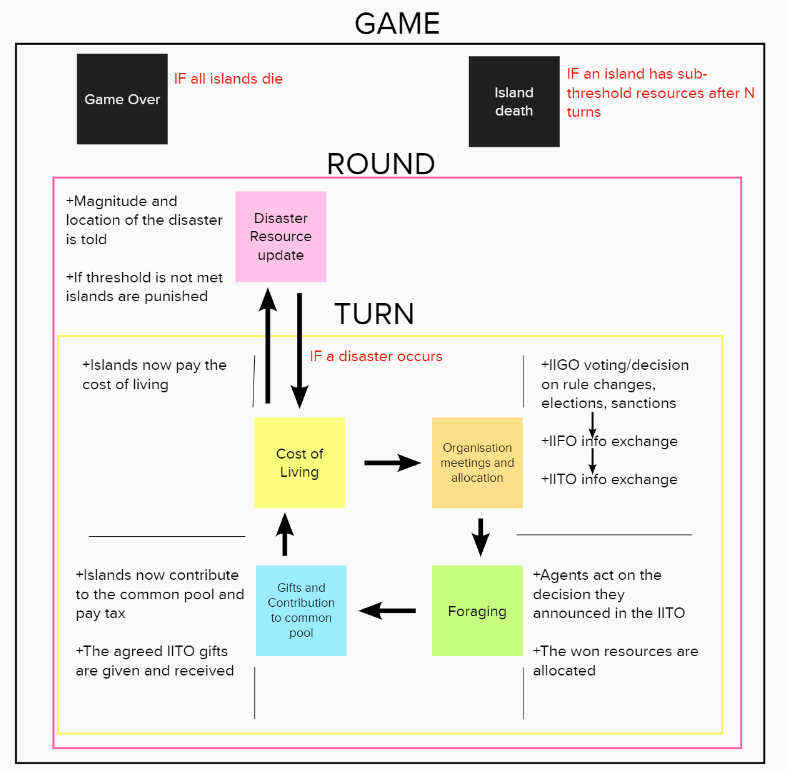
\includegraphics{03_gamedesign/images/gamespec-flow.png}
    \caption{High Level Game Specification Flow Diagram}
    \label{fig:gamedesign-flow}
\end{figure}

\subsection{Design Choice Justification}
Every action taken in the game adds to the dilemma placed on the agent to explore how they interact and attempt to overcome challenges through self-organisation. To complicate matters further, the meetings occur only to form agreements, which can also be broken after they are made. The allocation also occurs first to assist islands that are struggling by allowing them to take from the common pool immediately and use these resources to forage or, at a minimum, pay their tax.

\subsection{Game Parameters}
Many of the parameters within the game can be modified to adjust the difficulty of the game. It should be noted that some of these parameters have a greater impact than others. For example, the agents may or may not have access to the common pool threshold level and this knowledge, or lack thereof, will result in entirely different agent performance. This because each agent relies on different strategies and approaches each aspect of the game in a different way. For example, while some agents rely more on social strategies and cooperation to mitigate unknown risk, others rely heavily on calculations and predictions. Each agent strategy will come with its own unique set of benefits and limitations in the context of the game, performing better or worse, under different conditions.

% Start of section on implementation

\section{Implementation}
\label{sec:GD:implementation}

Implementation design was important as the majority of the class were involved in writing simulation code. As such, dedicated \emph{infrastructure} engineers from each team were elected to form an infrastructure team responsible for building the central part of the game, otherwise known as the \emph{server}. Each team's infrastructure engineer was tasked to own the implementation of a slice of the server.

One such sub-team was the \textbf{core} infrastructure team, responsible for building the core parts of the game server. Inputs were taken from the entire class to choose the best implementation strategies and design--a solid and simple core foundation was paramount to allow clean continuous integration of code and ideas from all contributors. The subsections below detail implementation specifics of the game's simulation.

\subsection{Architecture}
\label{sec:GD:implementation:arch}

The structure of the game was closely modelled after a \emph{client-server} model\footnote{\url{https://en.wikipedia.org/wiki/Client-server_model}}, but note ``closely''--whilst the nomenclature was taken directly from the aforementioned model, there are some differences. \emph{Server} and \emph{client} in this context bear the following definitions:

\begin{definition} \label{def:server}
    The \textbf{server} is the central game runner, responsible for initiating game events (such as a disaster or the start of a turn). Certain events require the actions of agents, in which the server will invoke a function on the agents to receive a response. Further, the server acts as a source-of-truth for the game's state.
\end{definition}


\begin{definition} \label{def:client}
    Each \textbf{client} is implemented by an agent. The client provides an interface of functions in which the server can invoke. Moreover, clients may also invoke certain functions from the server's interface to read specific game information.
\end{definition}

The major difference of this architecture to a traditional client-server model is that, in the former, the stateful central server drives the other clients (by triggering events and eliciting responses), as opposed to clients sending stateless requests to a server to receive a response in the latter. Furthermore, whilst the client and server have been separated architecturally, the entire system still operates as a single process.

\subsection{Technology Stack}
\label{sec:GD:implementation:techstack}

Agreeing on a technology stack proved to be challenging--the class had varying levels of programming expertise. Whilst Prolog\footnote{\url{https://en.wikipedia.org/wiki/Prolog}} and Qu-Prolog\footnote{\url{https://staff.itee.uq.edu.au/pjr/HomePages/QuPrologHome.html}} (an extension to the former) were used to cover topics in the lectures, the class did not favour them over more well-known and established imperative programming languages. Hence, time was dedicated to formulate a consensus to decide on the technology stack, with primary focus given on the choice of implementation language. Firstly, high priority requirements were defined for the stack:

\begin{itemize}
    \item Easy to learn
    \item Easy to setup
    \item Cross-platform
    \item Easily maintainable
    \item Friendly features
\end{itemize}

Minimum Working Examples (MWEs) comprising a single server and two clients were created in different stacks, which served as starting points for discussion among members of the class. The MWEs implemented are as follows.

\begin{enumerate}
    \item \textbf{Multi-language}\footnote{\url{https://github.com/SOMAS2020/somas-demo}}.
          A multi-language (C++ server with a Python and a C++ client) MWE was first set up. It was first thought that allowing agent teams to choose the programming language they were most familiar with would speed up development. However, despite this stack's benefits, it could not be easily made cross-platform. Each agent's code would need to be run in a separate process, and Inter-Process Communication (IPC) would be required to pass messages. IPC is quite low-level and varies vastly among different systems. Further, protocols for the IPC would also need to be set up to pass the correct message, and having no strong typing as in a strongly-typed language (or session-typed\footnote{\url{https://arxiv.org/abs/1906.03836}}) approach would make it difficult to maintain and develop.

    \item \textbf{Python}\footnote{\url{https://github.com/SOMAS2020/somas-demo-py}}.
          Python\footnote{\url{https://www.python.org/}} is widely used by the scientific community in recent years with the growing ubiquity of scientific computation packages available for it. As such, Python was a strong contender as most of the class already know Python from past projects. However, Python's weak typing meant it scored low on the ``easily maintainable'' part--the server and client interfaces would benefit a lot from strong typing. While add-on static typing tools such as \texttt{mypy}\footnote{\url{https://mypy.readthedocs.io/}} could be employed (it is also used in the MWE), it would still not be as powerful as built-in strong typing as in languages such as C\# and Go.

    \item \textbf{C\#}\footnote{\url{https://github.com/SOMAS2020/somas-demo-cs}}.
          C\#\footnote{\url{https://docs.microsoft.com/en-us/dotnet/csharp/}} is the flagship language of the .NET ecosystem. C\# shares a large part of its design to the more popular C++. C\# is strongly-typed, and promotes use of clean Object-Oriented Programming (OOP). Many of the features from C/C++ that can be \emph{dangerous} are not present or hidden, making it more beginner friendly. A drawback is that some experience with C-family languages is required to pick up C\# quickly.

    \item \textbf{Go}\footnote{\url{https://github.com/SOMAS2020/somas-demo-go}}.
          While most of the class was not familiar with Go\footnote{\url{https://golang.org/}}, its simple language syntax and highly-featured toolchain make it very easy to learn. The modern Go toolchain makes it extremely simple for programs to work cross-platform. While Go's omission of OOP and generics might be seen as a disadvantage, it makes it an easy language to learn, and prevents pitfalls commonly caused by such ``features''. Go, like C\#, is strongly typed. Moreover, Golang's great support for WebAssembly\footnote{\url{https://webassembly.org/}} would prove useful for visualisations, further detailed in~\ref{sec:GD:implementation:visualisations}. Another nice feature is that concurrency can be easily implemented in Go, which meant that agent actions could be run concurrently to speed up simulations.
\end{enumerate}

After discussion, scores (out of 10) were given for each stack. Table~\ref{table:techstackscores} shows these scores. The multi-language and Python approaches were removed from consideration--the former due to its low total score and the latter because of its low maintainability. The decision between C\# and Go was harder, and ultimately resulted in a \emph{simple majority} vote by the class. 37 people voted in total, with 25 in favour of Go. Hence, Go was finally chosen.

\begin{table}[h]
    \centering
    \caption{Scores given for each stack based on requirements}
    \label{table:techstackscores}
    \begin{tabular}{|c|c|c|c|c|c|c|}
        \hline
        Stack                     &
        \makecell{Easy              \\ to \\ learn}              &
        \makecell{Easy              \\ to \\ setup}              &
        \makecell{Cross-platform} &
        \makecell{Easily            \\ maintainable}             &
        \makecell{Friendly          \\ features}                 &
        \makecell{Final             \\ score \\ (out of 50)}
        \\
        \hline
        Multi-language            &
        6                         &
        2                         &
        0                         &
        2                         &
        10                        &
        20
        \\
        \hline
        Python                    &
        8                         &
        6                         &
        8                         &
        3                         &
        8                         &
        34
        \\
        \hline
        C\#                       &
        6                         &
        5                         &
        8                         &
        9                         &
        8                         &
        37
        \\
        \hline
        Go                        &
        8                         &
        8                         &
        10                        &
        8                         &
        6                         &
        40
        \\
        \hline
    \end{tabular}
\end{table}


\subsection{Visualisations}
\label{sec:GD:implementation:visualisations}

\subsubsection{Toolchain}
A benefit from the choice of the Go technology stack was that it supports compiling source code into WebAssembly out of the box. WebAssembly can be run efficiently in most modern browsers, which meant that in-browser simulations can be run and then visualised on a website.

The website (\url{https://somas2020.github.io/SOMAS2020/}) features... % TODO:- Vis team: yp717 et al.

\subsection{Engineering Practices}
\label{sec:GD:implementation:practices}

Developing and maintaining a codebase with contributions from around 40 developers was projected to be non-trivial. Therefore, good software engineering practices and rules were employed to be upheld by all contributors to make the process smoother and--where possible--automated.

\subsubsection{Code testing}

While Go is strongly typed and would mean that most errors can be detected at compile-time (or even at time of coding with its performant language server), having unit and integration tests greatly improved the maintainability and ease of development of the project--these issues were particularly important as this was a large-scale group software engineering project--developers stepping on each other's toes is a common occurrence in non-tested group project code. Henceforth, tests were required for non-trivial server-side code.

<<<<<<< HEAD
\subsection{Peer Review}

Peer review was also setup via GitHub pull requests--each change required the approval of another member in the infrastructure team. This practice not only promoted consistent code design and implementation, it minimised mistakes and ensured that the code implementation meets design and implementation requirements set forth. Further, as there was variation in programming skill among code contributors, knowledge sharing was facilitated by code reviews. This was also a critical opportunity for engineers to learn more about the other code being contributed to the project.

\subsection{Continuous Integration}
\label{sec:GD:implementation:practices:CI}

Via GitHub Actions\footnote{https://github.com/features/actions}, continuous integration was set up. Each Pull Request (PR) was set up to trigger automated runs of written tests and a full simulation in addition to static code analysers such as linters. These checks must all pass for the PR to be merged into the main branch. Automated testing and code analysis saved time and facilitates regression testing, as all tests--existing and new--were run for each change. Running a full simulation also served as a good stress-test for the system to make sure that it does not crash on a similar full simulation. Further, automated tests were run on a reference system (Ubuntu 20.04 with Go 1.15.5 and Node 14), helping to prevent system-specific quirks or bugs from polluting the codebase.

\subsection{Continuous Development}

On receiving PR approval, passing automated tests and finally merging into the main codebase, the visualisation website is automatically rebuilt with the latest changes. This saved time as manual builds were not required. The builds were produced on a reference system (identical to that mentioned in~\ref{sec:GD:implementation:practices}), ensuring consistent builds free from system-specific quirks. Further, automated builds meant that the website always runs on the latest codebase.
=======
\subsubsection{Peer Review}

Peer review was also setup via GitHub pull requests--each change required the approval of another member in the infrastructure team. This practice not only promoted consistent code design and implementation, it minimised mistakes and ensured that the code implementation meets design and implementation requirements set forth. Further, as there was variation in programming skill among code contributors, knowledge sharing was facilitated by code reviews. This was also a critical opportunity for engineers to learn more about the other code being contributed to the project.

\subsubsection{Continuous Integration}

Via GitHub Actions\footnote{https://github.com/features/actions}, continuous integration was set up. Each Pull Request (PR) was set up to trigger automated runs of written tests and a full simulation in addition to static code analysers such as linters. These checks must all pass for the PR to be frequently merged into the main branch. Automated testing and code analysis saved time and facilitates regression testing, as all tests--existing and new--were run for each change. Running a full simulation also served as a good stress-test for the system to make sure that it does not crash on a similar full simulation. Further, automated tests were run on a reference system (Ubuntu 20.04 with Go 1.15.5 and Node 14), helping to prevent system-specific quirks or bugs from polluting the codebase.

\subsubsection{Continuous Deployment}

On receiving PR approval, passing automated tests and finally merging into the main codebase, the visualisation website is automatically rebuilt with the latest changes. This saved time as manual builds were not required. The builds were produced on a reference system (identical to that mentioned in the Continuous Integration section), ensuring consistent builds free from system-specific quirks. Further, automated builds meant that the website always runs on the latest codebase.
>>>>>>> 962869f9957a17b0764e8a570c39fa55a16b5576

    \chapter{Environment}
\section{Foraging}

\begin{definition} \label{def:Welfare}
\textbf{Welfare} is the state of wealth, it can either be personal or collaborative (social).
\end{definition}

\begin{definition} \label{def:Maximising Social Welfare}
\textbf{Maximising Social Welfare} is a strategy which attempts to maximise the total amount of welfare (resources) the islands have.
\end{definition}


\subsection{Foraging Background}

Foraging is a fundamental requirement that is needed as it is a method of obtaining more resources from the starting amount. Foraging is based on the concept of inputting resources to get a return.

\subsubsection{Underlying Concept}

The primary objective of foraging in this game is to introduce a dilemma to the agents in order to investigate their behaviours and whether they work together despite different personal goals. Including two methods of foraging promotes decision making among the islands, allowing for strategic interactions to maximise personal benefits while still reaching the overarching goal of survival. 

The inspiration for our concept of foraging comes from the stag hunt game. Thus, it introduces elements from it. Specifically, this approach results in a game with \textbf{no dominant strategy} and in which \textbf{an agent's choice can impact another agent's}.

The process of stag hunt is that each agent selects a method of hunting without the information of the other agents. The social welfare (total payoff) is significantly reduced if their choices differ. The selection of stag suggests that the agent is going for higher \textbf{payoffs} whilst the selection of hare indicates that the agent is \textbf{risk aversion} as both agents are required to stag hunt to get any personal welfare (see Definition~\ref{def:Welfare}).

\subsubsection{Modifications to the Original concepts} 
A few changes have to be made to make this dilemma viable for our multi-agent system, in addition to adding realism. 

\begin{enumerate}
    \item The dependency was changed to be based on the input resources rather than the number of islands participating. This added a more realistic element to the dilemma as in reality a hunt’s return would be based on the amount of resources (different possible resources: people, food, water and materials) entered rather than the number of islands participating.
    \item Instead of a specified return, probabilistic return was implemented which adds a randomness element to the game to prevent pattern recognition. These probabilities can be tied to the population, disasters, forecasting and number of animals hunted.  
\end{enumerate}

Furthermore, the dynamics of our agents and allowing for a more complex decision-making interaction between islands and the environment have been explored. It is worth mentioning that some of these design ideas were implemented in the coursework. These changes have been made to make foraging more volatile and unpredictable, adding to the complexity of the system, allowing the teams to further evaluate the agents’ performance on observing and to use learned knowledge to take action.

\subsubsection{Tier System}

The deer hunting and fishing is divided into tiers, which depend on the total amount of input resources. Tiers represent the number of fish that can be caught in a given day, and the “zero” tier represents the cost associated with getting to the hunting location. Beyond the zero tier, the cost of catching another deer or fish will decrease as it is easier to catch the second animal than the first one, since the agents have already arrived at the hunting location. Therefore, if the agents do not even enough to reach the first tier, then they wouldn't get any returns. It should be noted there is a limit to how many animals the agents can catch in a given day.

The focus of fishing is to avoid risk at the expense of payoff. This means that all tier requirements are lower than those for the deers. However, the return is also lower thus if only one island goes fishing they are still expected to have a low return as long as they have enough resources to catch the first fish. Thus, the benefit of deer hunting is higher payoffs. However, these improved returns come at the cost of significantly higher tier thresholds. Therefore, it is possible for a single island to go deer hunting without enough resources to reach the hunting location leading to no return.

\begin{equation}
\text{Increments of catching $n$ animals}=
\left( \begin{array}{ll@{}}
n=0 \longrightarrow \Delta^0 = 1 \\
n=1 \longrightarrow \Delta^1 = 0.8^1 \\
n=2 \longrightarrow \Delta^2 = 0.8^2 = 0.64 \\
n=2 \longrightarrow \Delta^3 = 0.8^3 = 0.512 \\
n=4 \longrightarrow \Delta^4 = 0.8^4 = 0.4096\\
\end{array} \right) 
\label{eq:Cumulative Cost 1}
\end{equation}

\begin{equation}
\text{Utility Tier Cost}=\ \sum_{n=0}^{n} \Delta^{n} = \Delta^{0} + \Delta^{1} + \Delta^{2} + \Delta^{3} + \Delta^{4} + ....
\label{eq:Cumulative Cost 2}
\end{equation}

Equation~\eqref{eq:Cumulative Cost 1} and Equation~\eqref{eq:Cumulative Cost 2} show the formulation of the decay function for tier system. The tier system is shown in the Figure~\ref{fig:Foraging Tier System} where $n$ stands for the tiers, with decay costs ($\Delta$) of $0.8$ for the deer hunt and $0.6$ for fishing.

\begin{figure}[!htb]
    \centering
    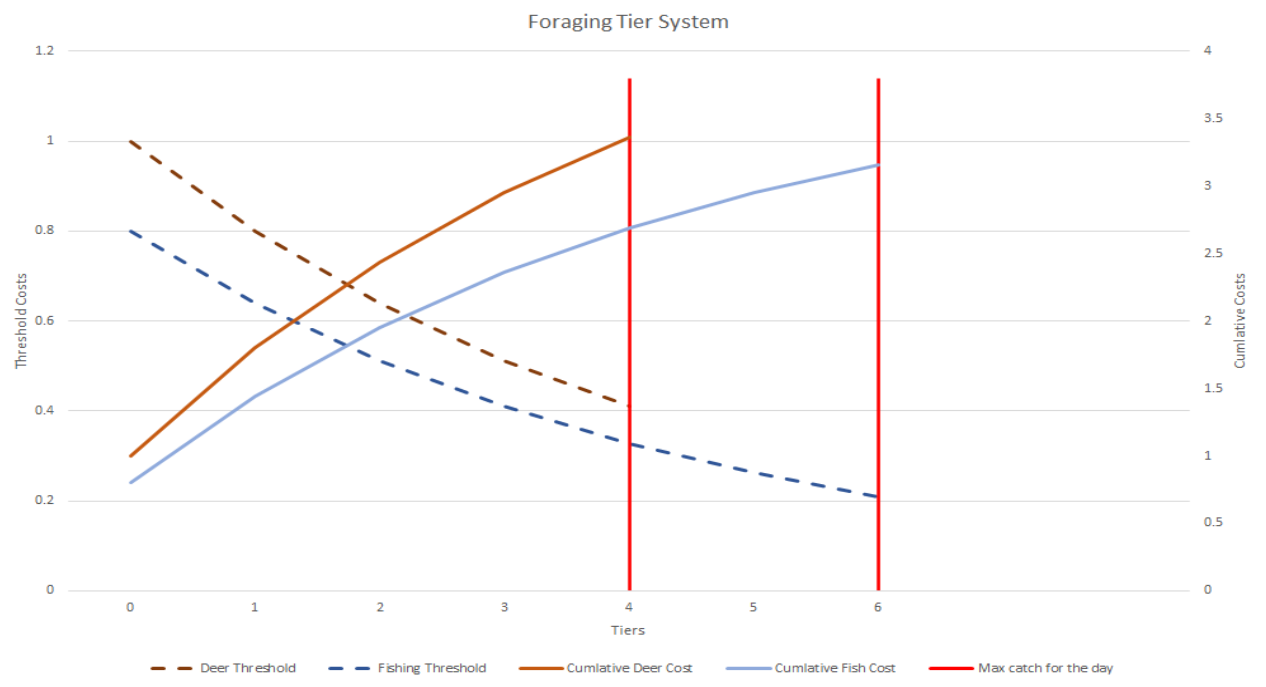
\includegraphics[width=0.9\textwidth]{04_environment/images/Foraging Tier System.PNG}
    \caption{Foraging Tier System}
    \label{fig:Foraging Tier System}
\end{figure}

The amount of resources inputted is scaled using a variable and the tiers are then calculated with them, the higher the tiers the lower the cost to catch the next animal. However, the total cost increases up to a daily catch limit. This means that if teams collaborate, they can invest less as individuals to get a collectively greater return through deer hunting. If they invest too much, then they will over spend as they reach the daily catch limit. As a result, it is more beneficial for some teams to go fishing because it has a higher daily catch limit, although it comes with lower returns. In other words, there is a need for some self-sacrifice to reach the maximum welfare (see Definition~\ref{def:Welfare}). Moreover, fishing is a similar foraging method with the key difference being that it utilised a normal distribution and the start of the tiers.

\subsection{Example Distribution}
\subsubsection{Example of the Distribution for Foraging Return (Deer Hunting - Payoff Dominant)}

\begin{figure}[!htb]
    \centering
    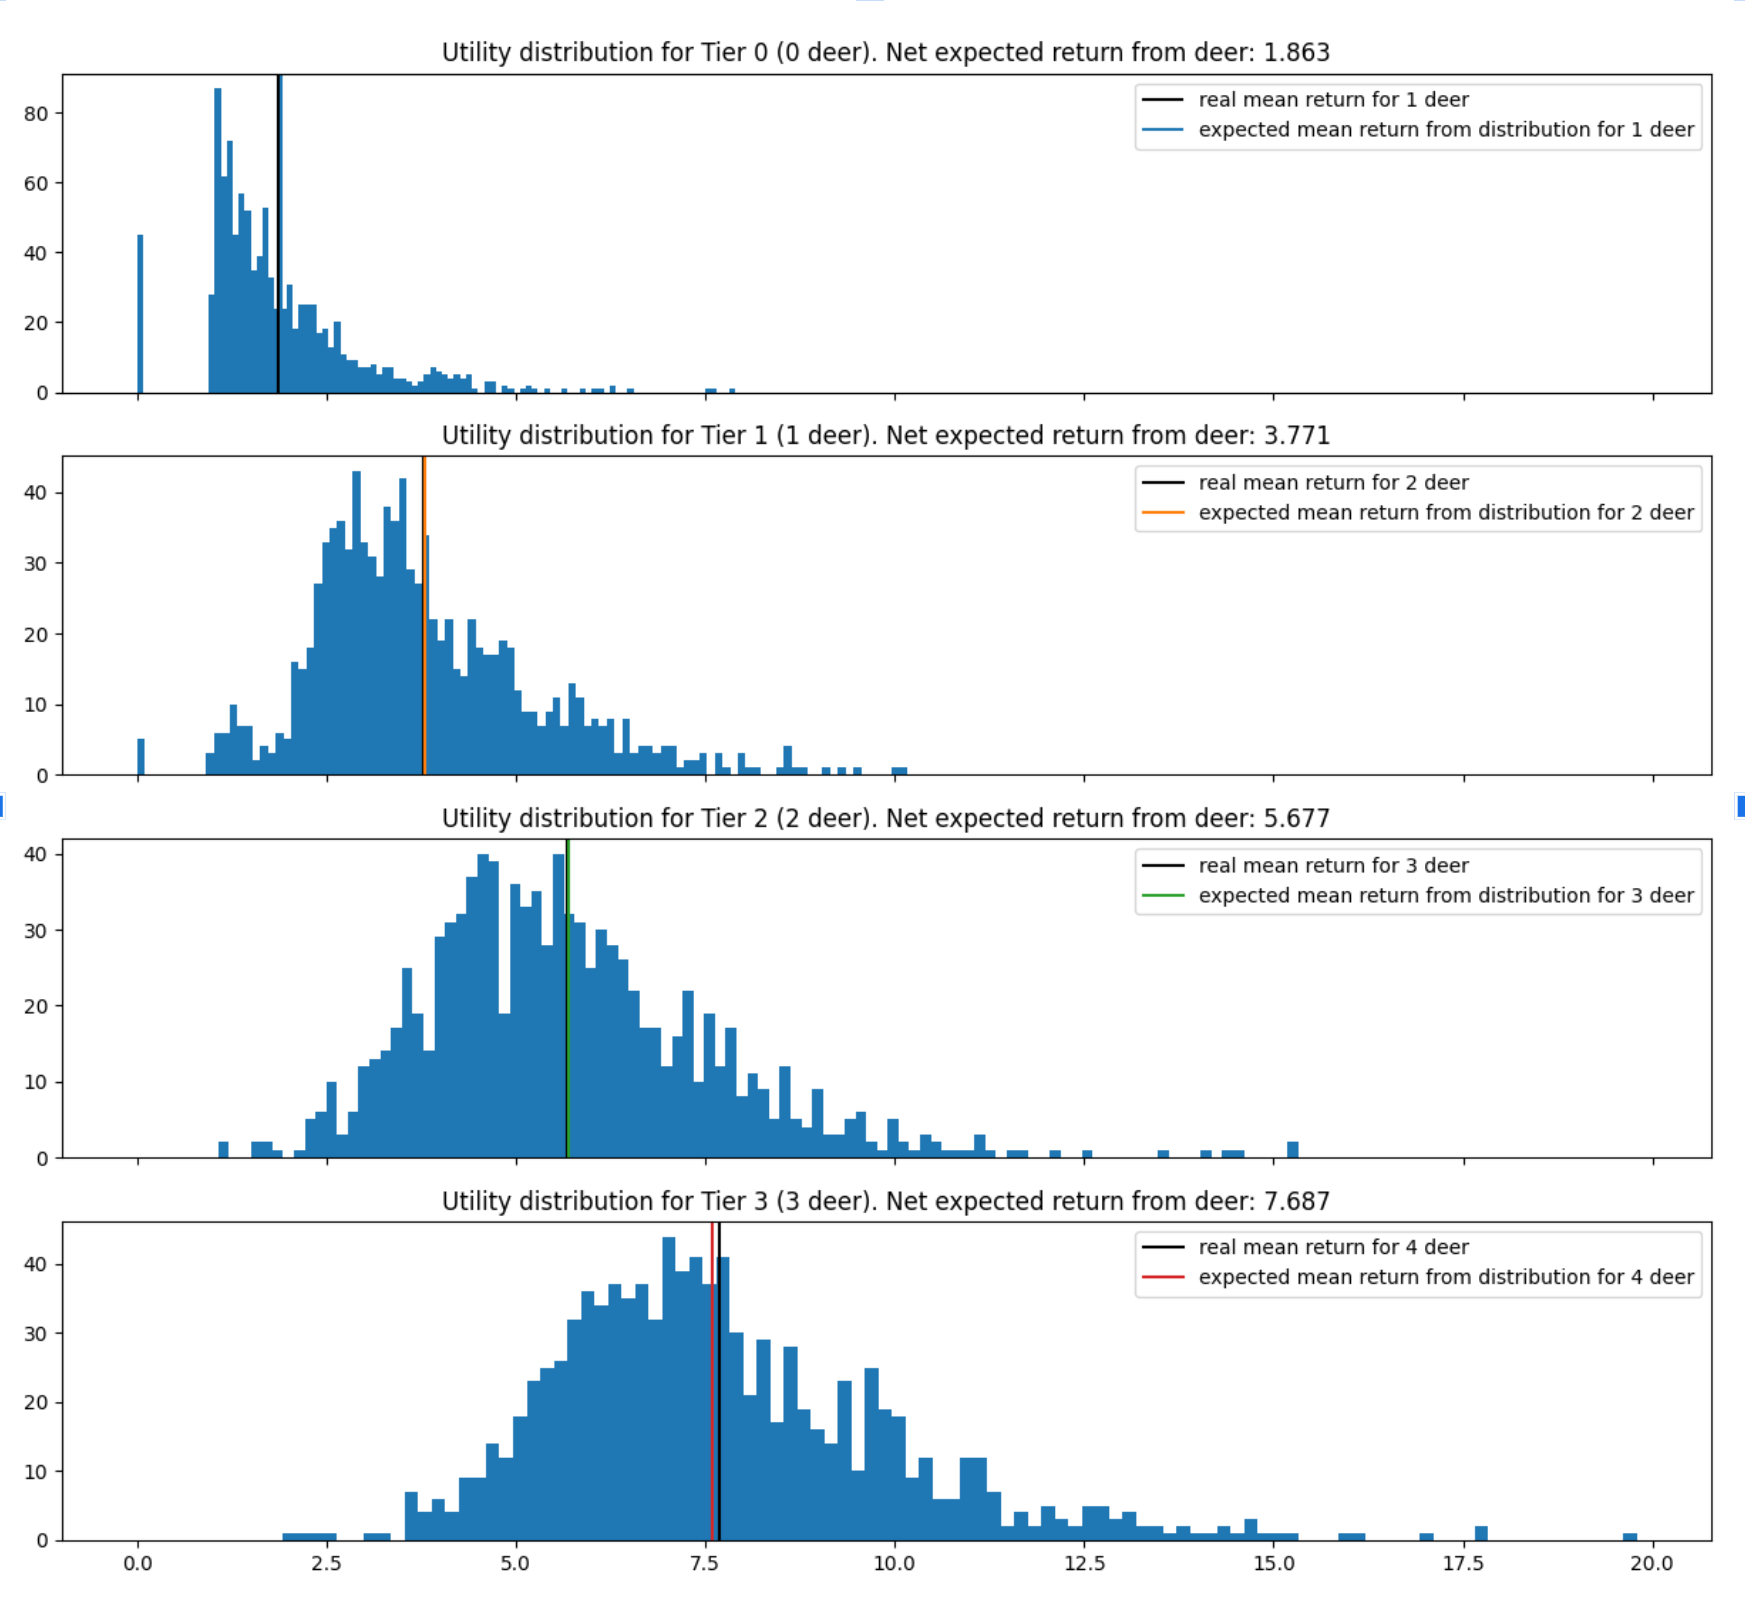
\includegraphics[width=1\textwidth]{04_environment/images/Distribution of Foraging returns Deer Hunting.PNG}
    \caption{Deer hunting payoff dominant Distribution for foraging return}
    \label{fig:Distribution of Foraging returns Deer Hunting}
\end{figure}

To increase the risk of deer hunting, a Bernoulli Random Variable ($D$) was used to prevent guaranteed resource returns after a hunt. While the Exponential Decay ($W$) is to disincentive too much resources being placed in hunting and hoping for a high return. However, this all comes with the benefit of significantly higher ($2\times$) returns than fishing.

Figure~\ref{fig:Distribution of Foraging returns Deer Hunting} represents the return utility which will be multiplied by an output scale to give the return payoff. The Figure~\ref{fig:Distribution of Foraging returns Deer Hunting} shows the average \textbf{expected mean} return utility, in colour, after $1000$ iterations which is close to the \textbf{real mean}.

\newpage
\subsubsection{Fish hunting - Risk Aversion}

Fishing is similar to Deer hunting, except that it uses only a Normal Distribution ($F$), which focuses on avoiding risk by being very predictable and safe. Figure~\ref{fig:Distribution of Foraging returns Fishing} illustrates the return utility for fishing.

\begin{figure}[!htb]
    \centering
    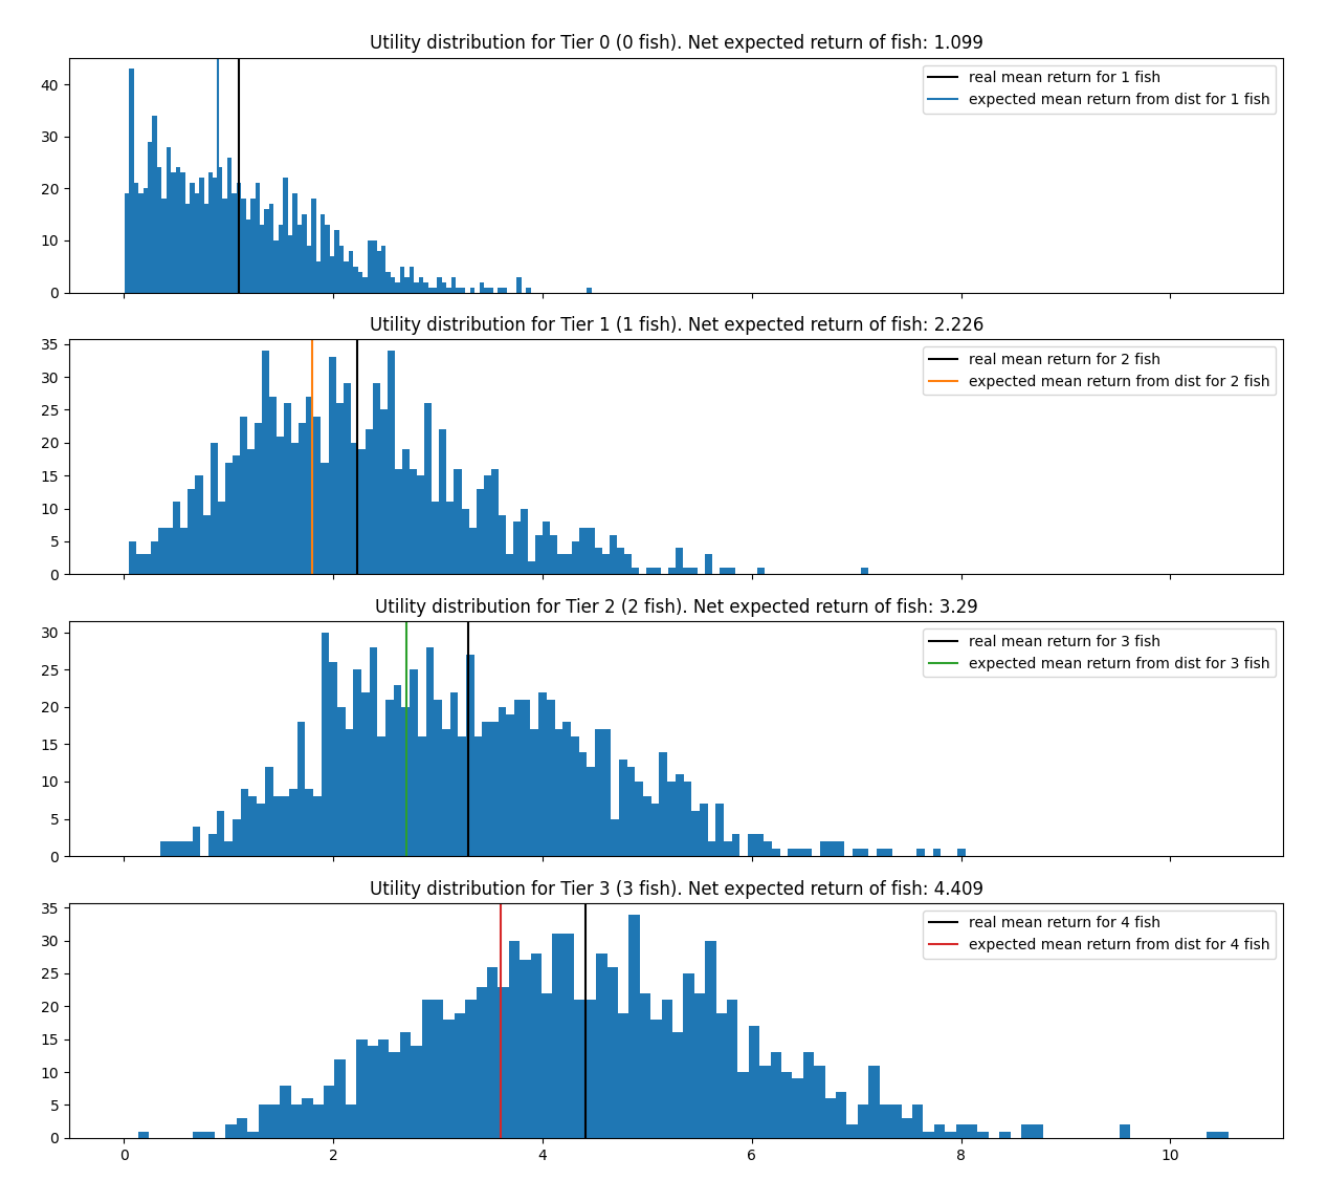
\includegraphics[width=1\textwidth]{04_environment/images/Distribution of Foraging returns Fishing.PNG}
    \caption{Fishing Risk aversion Distribution for foraging return}
    \label{fig:Distribution of Foraging returns Fishing}
\end{figure}

As seen in Figure~\ref{fig:Distribution of Foraging returns Deer Hunting}and Figure~\ref{fig:Distribution of Foraging returns Fishing}, the return for the deer is almost double that of the fish return whilst the fish return is much easier to obtain due to the lower cost of catching fish.

\newpage
\subsection{Solution Concepts}
\subsubsection{Dominant Strategy}

In this implementation, there is no dominant strategy. Therefore, if an agent decides to go deer hunting, whereas all the other islands are fishing, that agent would not get the best return possible. Hence it is not the best strategy. Whilst if an agent goes fishing and there are a sufficient amount of agents deer hunting, then that agent would be passing on the opportunity of to gain a larger return in deer hunting. Hence, it is not the best strategy either.

\subsubsection{Nash Equilibrium}

In the regular stag hunt game, there are two pure Nash Equilibria, where both agents go for either payoff or risk aversion. In our implementation, there are multiple Nash Equilibria. These are the points where the islands cannot benefit themselves by moving to deers hunting to generate more return. As there is a limit to how many deers that can be hunted thus by moving to deer hunting they are getting a worse return than if they just stayed at fishing. Whilst the islands at the deer hunt are already making a greater return and have no reason to switch to fishing.

\subsubsection{Pareto Optimal Strategy}

At some point, all agents will be in a position where changing foraging methods will not yield any better income for themselves and in fact also hinder others. This is due to the max daily deer hunt limit which creates a maxim return on the deer hunt. Therefore there will be points where the islands will change as the amount of resources being entered into both methods of foraging is the most efficient, this being where deer returns are maximised. There may also be a point where the agent can benefit by switching away from deer hunting. However, this will cause the other islands in the deer hunt to have a worse pay off due to a possible drop in tier resulting in worse returns.

\begin{figure}[!htb]
    \centering
    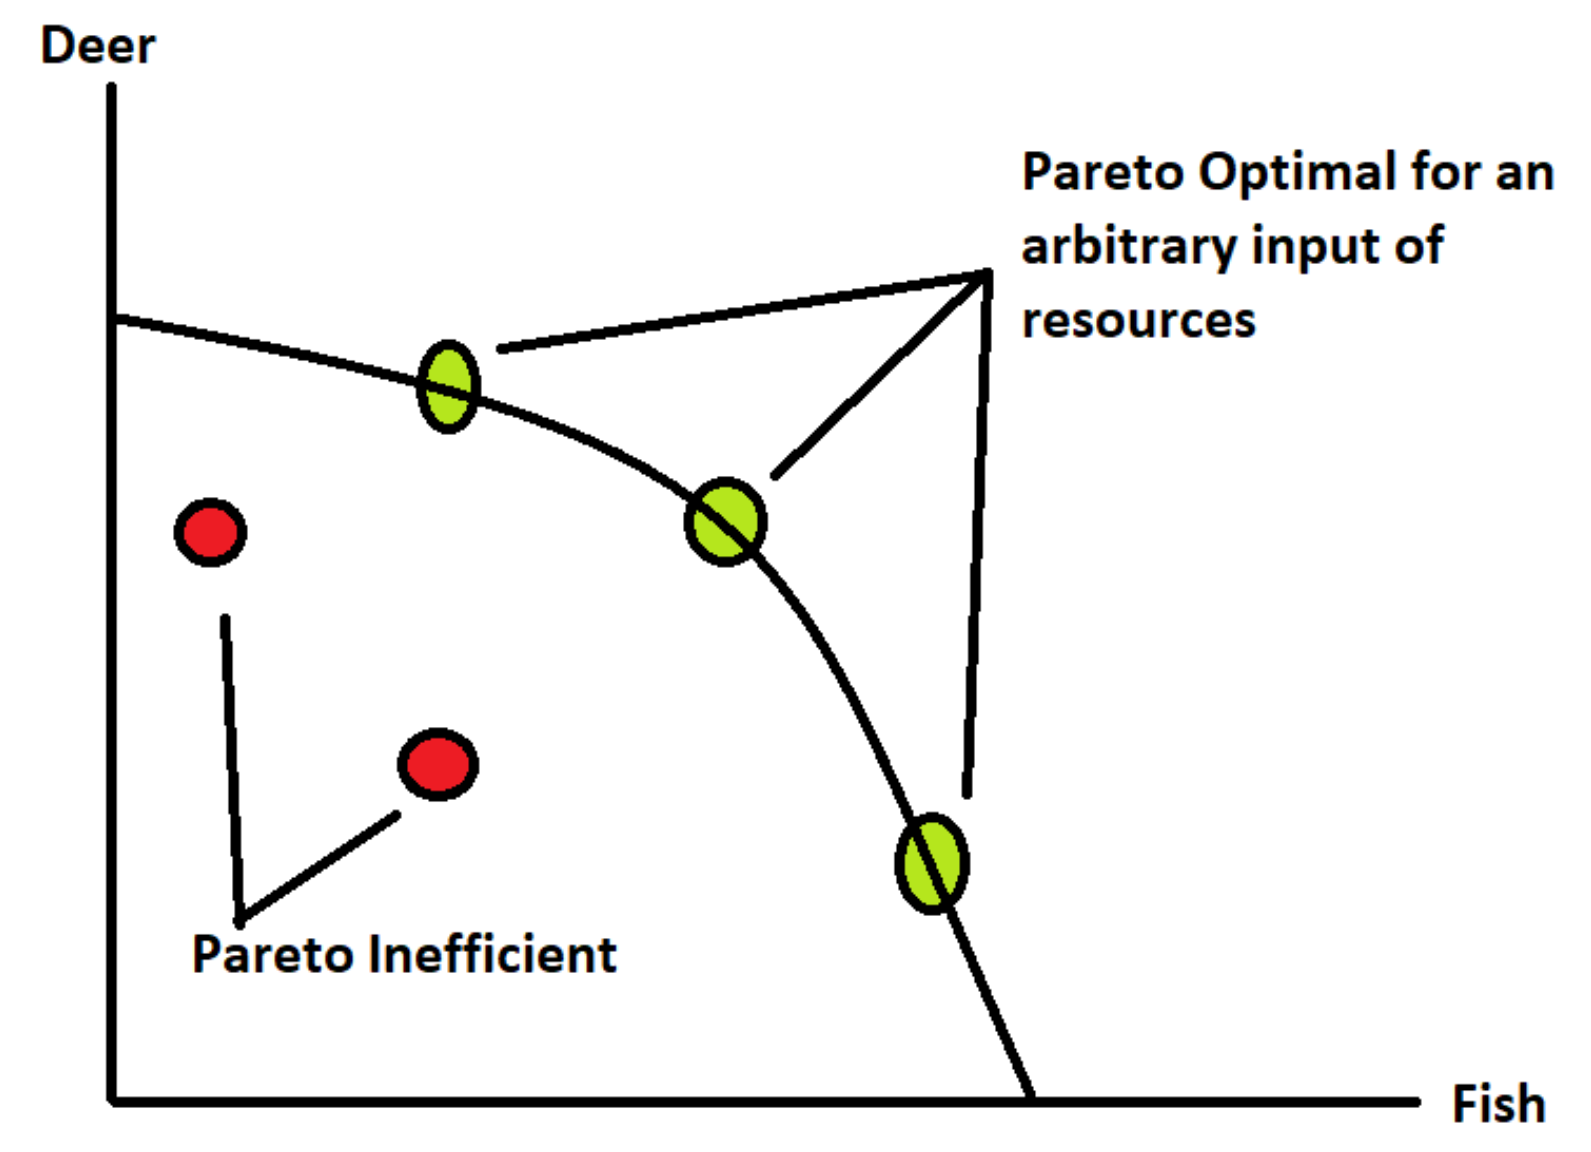
\includegraphics[width=0.7\textwidth]{04_environment/images/Pareto Optimal Strategy.PNG}
    \caption{Pareto Optimal Strategy}
    \label{fig:Pareto Optimal Strategy}
\end{figure}

\subsubsection{Social Welfare Maximisation}

It is possible for these islands to find the social welfare maximum (see Definition~\ref{def:Maximising Social Welfare}) in this foraging function with enough time. The islands could identify the exact amount of resources needed, for both fishing and deer hunting, to achieve the best return according to the maximum number of animals. Thus, by cooperating who goes where and spends how much, they are able to maximize their returns without spending more resources than necessary.

\subsubsection{Population Density}

Introducing a model that controls the population density of deer allows us to increase the complexity of the foraging function. In short, the deer hunting capacity decreases with decreasing population and increases with an increasing population. This then influences the maximum deer per hunt parameter ($n$), which in turn results in a more complex return calculation function (\texttt{\textbf{DtotalReturn}}), which would make it harder for agents to figure out forage tier boundaries to optimise their strategies.

The population change can be dynamic depending on various environmental factors, fetched from the rest of the system. For example, a disaster could supposedly cause the population density of deer to halve, making it harder to forage and therefore, causing lower returns. In this current implementation, a single species population model and more specifically logistic modelling for the deer and fish population was implemented. 
The model is described in Equation~\eqref{eq:Population Density}.

\begin{equation}
\frac{\mathrm{d} P}{\mathrm{~d} t}=k(N-P)
\label{eq:Population Density}
\end{equation}

\begin{itemize}
    \item $P$ is the total population. 
    \item $N$ is the maximum deer population (carrying capacity\footnote{The maximum population size of a biological species that can be sustained in a specific environment.}).
    \item $k$ is the growth coefficient.
    \item $t$ is time.
\end{itemize}

In Figure~\ref{fig:Deer population over time}, the simulation of the implemented logistic model can be observed, with a growth coefficient of $0.2$ and $N$ of $8$. It can be seen that there is an unpredictable pattern to population changes, which would be interesting to see affecting the tier system and in extend, the deer and fish foraging strategies of the agents.

\begin{figure}[!htb]
    \centering
    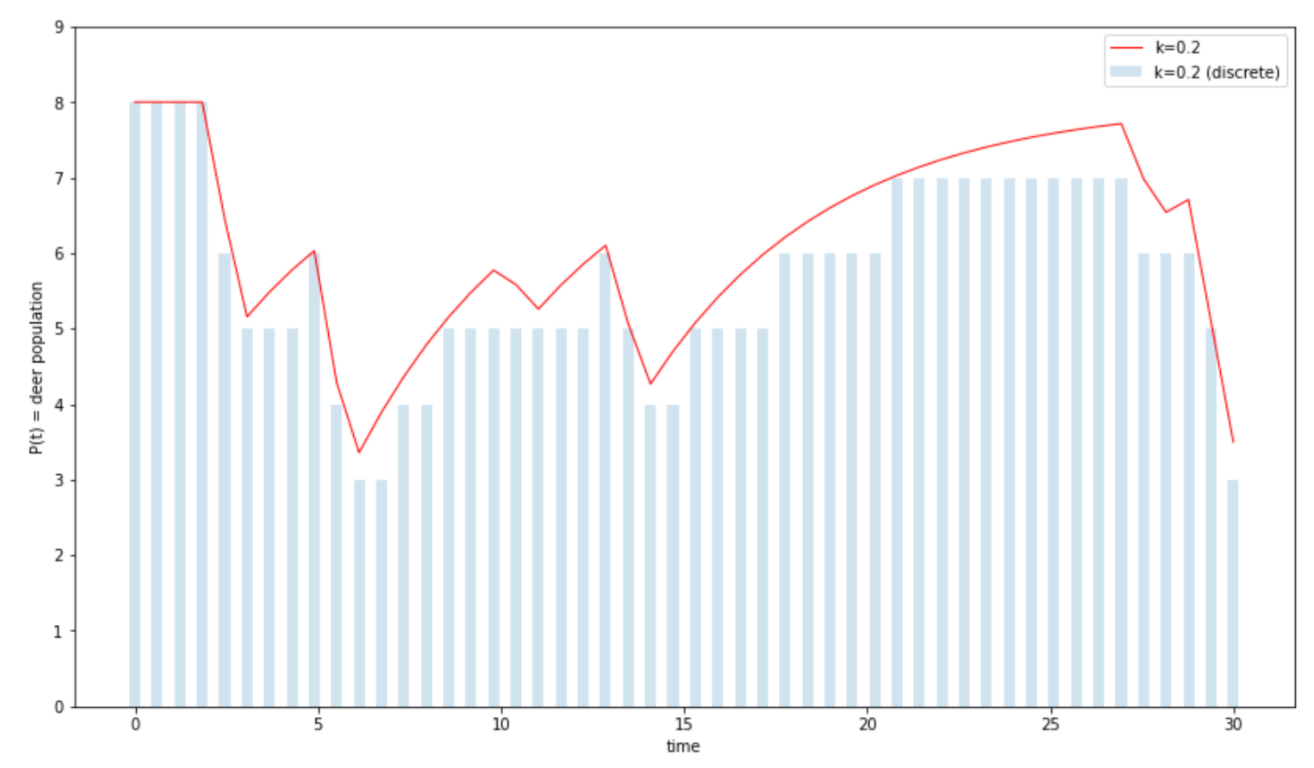
\includegraphics[width=1\textwidth]{04_environment/images/Deer population over time.PNG}
    \caption{Deer population over time (turns) under Logistic modelling with a growth coefficient of 0.2.}
    \label{fig:Deer population over time}
\end{figure}

Furthermore, In our implementation, $k$ and $N$ are constants. 

Modelling the population (or linking it to other environmental elements) allows us to make sure that the system’s dynamics are varying, making it harder for islands to settle onto a single foraging method because it always results in better returns. Pareto optimality is therefore harder to achieve and thus maximising social welfare (see Definition~\ref{def:Maximising Social Welfare}) is trickier, requiring agents to make more informed decisions, recognizing possible patterns. Of course, that would be an easier task for the islands, if they had knowledge on what is affecting the population (i.e. disasters), whereas a logistic model function might be more abstract in the eyes of our agents, requiring more processing. 

\subsubsection{Method of Resource Allocation}

Moreover, there is a parameter to allow either an equal split of returns after foraging regardless of the input, or a proportional split dependent on the amount of resources inputted by each island. Both of these implementations work in accordance to the previous specification. Such change allows us to observe the concept of free-riding further, looking at how greedy islands behave in the case of uniform resource returns.

The distribution method is based on two scalars. The first scales the inputs to the tiers, allowing the agent to choose how much they wish the tiers to cost. After which, the number of fish or deer caught is chosen by the tiers which goes into their respective distributions. The output of these distributions are then multiplied by the output scale. This allows the user to adjust the return amount each island can obtain, the output scalar should be above the cost of living in order to ensure the islands have enough resources to survive.  

\subsection{Future Work}

Further work could be done to make sure that there is enough complexity to explore the dynamics of our agents. Due to the project’s time constraints, some interesting ideas were not implemented but were thoroughly examined during the design process.

An important add-on to our previous implementation could be the enforcement of laws by the IIGO for the number of islands that can go foraging. That would introduce the need of internal agent relationships, adding another level of decision-making complexity to the agents. The specific alteration could result in some interesting findings. For example, there could be an auction scenario where islands would bid with their input resources, where only the highest bidders would be able to forage, as limited by the IIGO. Therefore, the islands with the lowest resources would be out-bidded, possibly causing a long-term resource depletion that would need to be mitigated by the more resourceful islands later in the game. It would be interesting to see how such change would affect the free-rider problem and how islands would adjust their strategies to out-bid other islands.

Another change that could be made is to let islands choose who they want to forage with. The islands would communicate with each other in form of direct messaging or voting to reach a decision. 
Essentially, our speculation is that agents would avoid the free-riding problem in both cases by enabling agents to make collective decisions based on communicated resource contributions. That’s because free-riders would be out-voted or not invited for foraging. That, in combination with the aforementioned tier system, would possibly result in all the islands contributing as much as possible to the input foraging “pool”. However, it would be interesting to see if islands can then reach Pareto optimality, where every single agent gets the best possible return for their input.

In addition to the above suggestions, agents would be restricted to just a single foraging area where they would only be allowed to forage with one neighbouring island using a ranking algorithm. This could alter the game's dynamics as an agent would only have limited partners (i.e. other islands) to forage with i.e. other islands in the same limited area. The aforementioned islands could be explicitly decided or randomly allocated. This could also be enforced and implemented as future work. Moreover, this particular scenario could be extended by programming prey densities to be geo-focused, where prey populations could vary between regions on the “map”. Islands would then need to make a strategic plan on how their ranking of neighbouring islands would change in accordance to their returns and returns broadcasted from other island pairs.

As discussed earlier, the population density of deer is a parameter that allows us to increase the complexity of the foraging function, tying it up to a realistic population model. It would be interesting to see what would happen if the growth coefficient increases, causing a population growth and observing the islands’ dynamics. Will they keep on “investing” higher resources each turn, taking advantage of the deer and fish abundance, or will they stick to their original, safe and static strategy?

In addition, going into resource allocation, the utility is in fact multiplied by an output multiplier. Therefore, the user determines the output multiplier value, as well as the resource allocation. Thus, agents can receive either a proportional split or an equal allocation of resources based on the users' decisions. Moreover, a few questions that be could be asked about the islands relationship and behaviour are: Will the islands seek to minimise inputs and benefit from the more generous islands, even at the cost of being allocated a lower tier? Will they input just enough to maximise the tier they are foraging in? Or, will they observe other island’s previous contributions and make a decision based on that?

Finally, more foraging options could be added in future implementations. For example, a third foraging technique; whale hunting could be created. This option would have an even higher return than deer hunting, deeming it an appealing forage method. The barriers of entry could be similar to that of the deer hunting method in this scenario but at the same time, there would be a more spaced out/expensive tier system. This combination would potentially incentivise cooperation between islands, if their strategy was to maximise returns. Also, as additional foraging methods have been introduced, the type of return was fixed for each foraging method and observe how agents decide to behave. For example, the deer and fish hunting methods result in returns proportional to inputs, whereas the whale hunting method would result in an equal split of returns between all participating islands. Would this mean that islands choose a fairer division of returns and not go on whale foraging at all? Or would they be intrigued by the higher costs and choose whale hunting over the other foraging methods? In the latter question agents would need to take into account that an island may enter an insignificant amount of resources and reap a large return. It is therefore up to the islands to decide if the higher payoff is worth the risk of other islands free-riding.

All the aforementioned behaviours are, of course, influenced by the island tactics. Therefore, an island programmed to be greedy could not cease to be greedy, no matter how the surrounding islands’ behaviours change, unless the greedy island can adapt. Therefore, agent strategies must attempt to draw conclusions on specific foraging methods and modify their strategies where appropriate.

\newpage
\section{Disaster}
\subsection{Disaster Background}

A game was designed, where agents directly confront a disaster and its risks once every round. This subset of the game creates a dilemma, where each island (agent) has to survive. They will have the opportunity to work together by investing collectively to the common pool, the disaster will be mitigated if the islands invest enough resources to reach a desired threshold. Otherwise, the islands would face negative impact, which would diminish their available resources. It is worth mentioning that the disaster will first extract resources from the common pool, and then if not enough resources have been invested, resources will be depleted from each island proportionally to their island’s damage.

Furthermore, the disaster was designed to comprise of an epicentre (eye of the storm), which is limited within the archipelago bounds, it is represented using Cartesian coordinates (EpiX, EpiY). Therefore, all islands or a subset of islands may be affected due to their proximity to the disaster epicentre. The island’s proximity to the disaster epicentre is directly proportional to the island’s damage. In other words, the island's available resources will be diminished based on the disaster magnitude and its location with respect to each island’s fixed location.

The following example can briefly explain the dilemma:

The closest an island from the eye of the storm, the larger the severity on that island. Therefore, the more resources are depleted. Let’s say the disaster epicentre hits around Island 1 as shown in Figure~\ref{fig:Disaster eye of the storm severity} and that the desired common pool threshold has not been met. Island 1 would be experiencing severe damages , and Island 2 and 6 some damages and the other islands low to no damage. Therefore, Island 1, 2 and 6 have the risk of not surviving if they are lacking resources, whereas Island 3, 4, and 5 would not be affected as much by the disaster.

\begin{figure}[!htb]
    \centering
    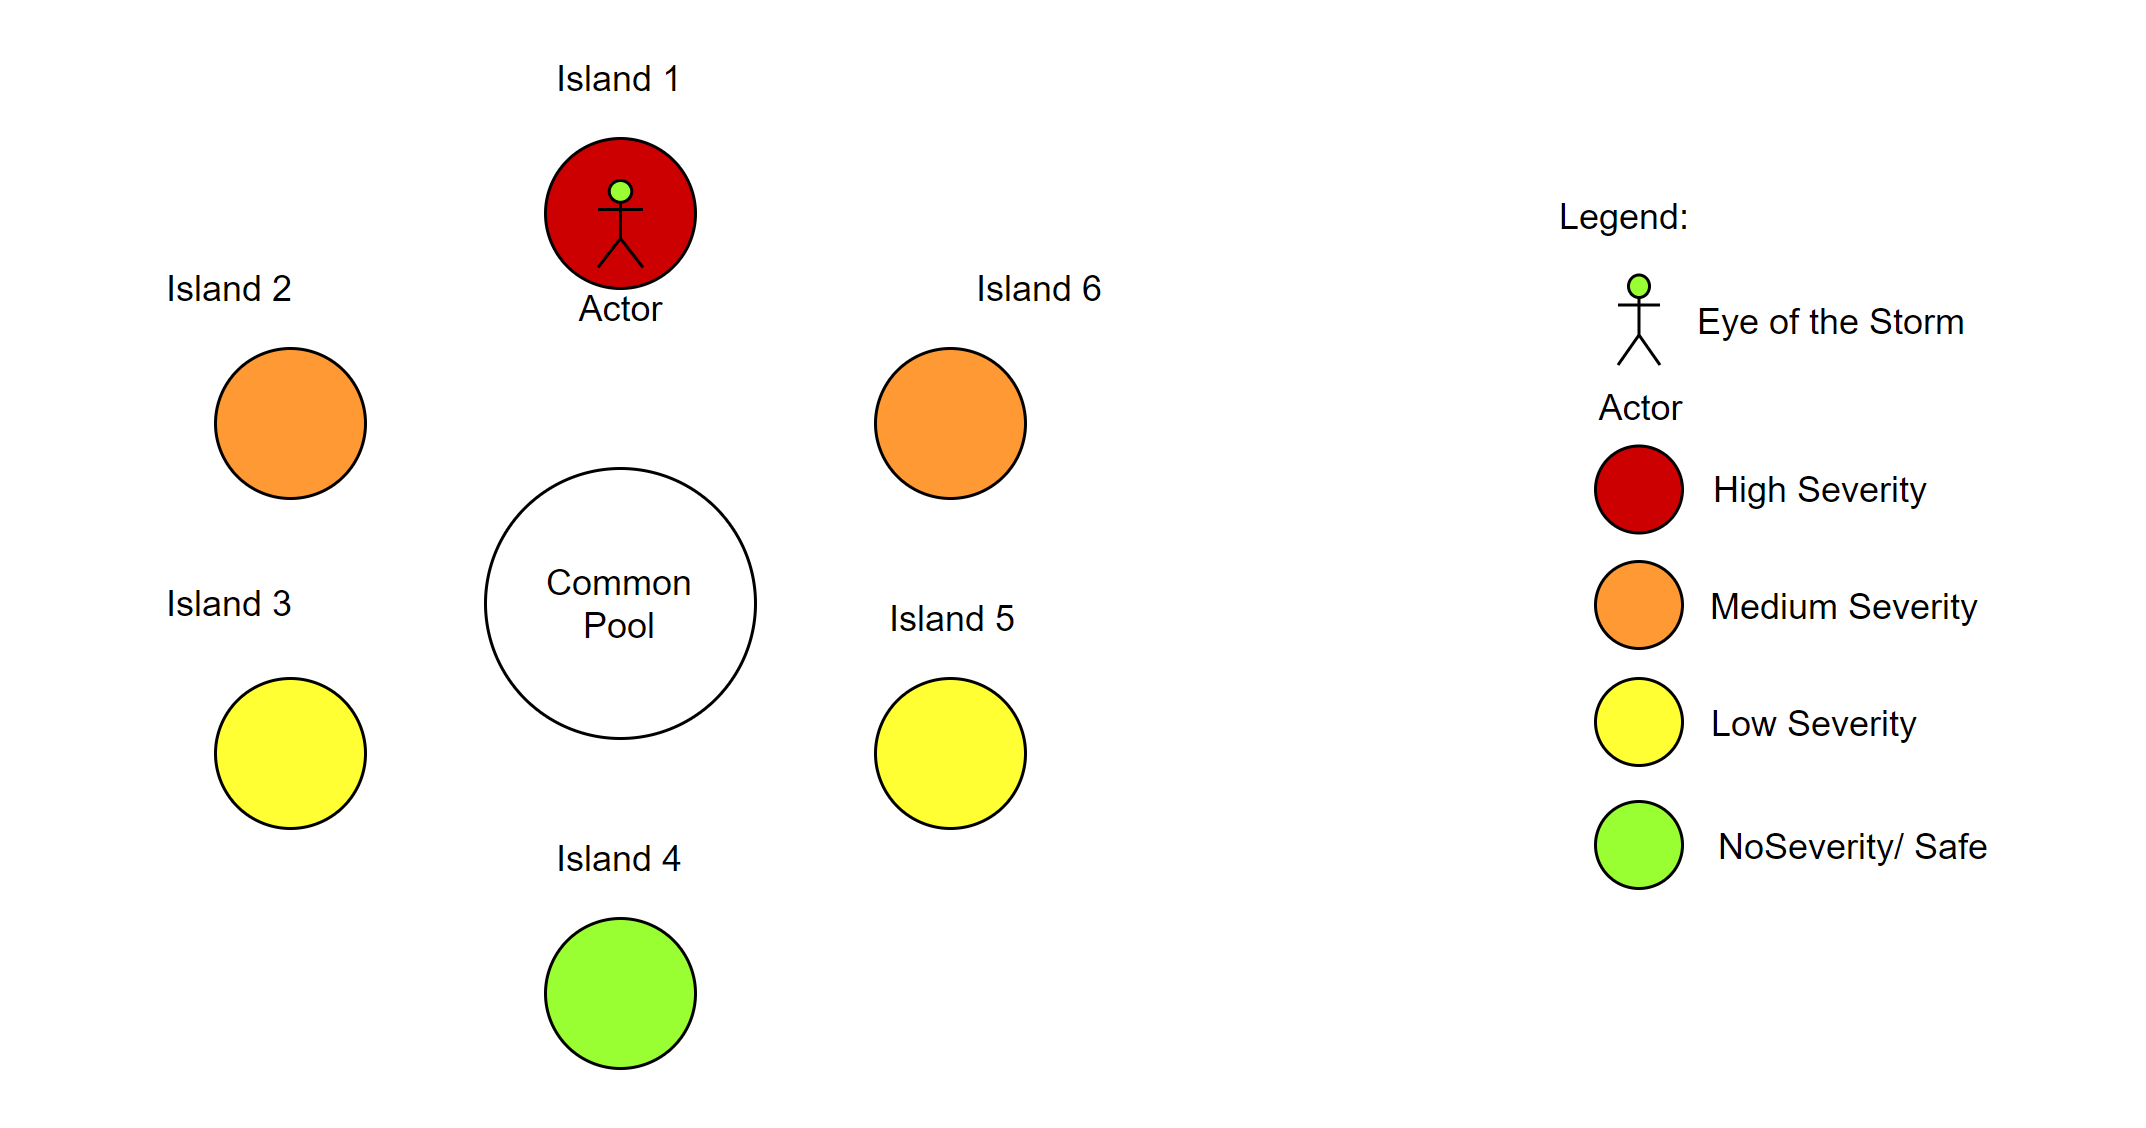
\includegraphics[width=1\textwidth]{04_environment/images/Disaster eye of the storm severity.PNG}
    \caption{Disaster Epicenter effects}
    \label{fig:Disaster eye of the storm severity}
\end{figure}

\newpage
\subsection{Future work}

There are multiple future work ideas that would be developed in the design aspect such as; a deterministic disaster which would be  designed as a straight line that accumulates during the days, once the threshold was met then the disaster would occur. Another deterministic disaster idea would be to link the disaster’s magnitude to time. Thus, agents would have to learn from past disaster occurrences, creating a memory. Agents would start learning from past disasters and would be able to forecast the next one. Therefore, the agents would be able to forecast that if a disaster did not surface for a long period of time, then the magnitude of the next disaster will be much larger than the previous one.

Another idea is that agents can invest into forecasting. Therefore, agents will have access to a history of past disasters, which would be utilised to learn and gain knowledge in order to predict the upcoming disasters.

Thus, the more resources invested by the agents in forecasting, the more disaster history data will be provided. This would enable the agents, to apply machine learning techniques to such data, allowing them to acquire more accurate and precise predictions of future events and develop better risk assessments. Therefore, agents will acquire knowledge, when investing in any of their resources.


\section{Common Pool}
\subsection{Common Pool Background}

A game was designed where one group of six islands (agents) have access to a common-pool resource. In micro-level, each island intends to maximise its utility while in macro-level, all the islands want to maintain sustainability and be protected by the upcoming disaster. The above description specifies a collective action problem where n-agents (six in our case) are seeking access to a common pool resource that is sufficient to satisfy some agents but not to satisfy all of them.

A Linear Public Goods (LPG) Game was implemented, where all the agents individually own some resources and try to maintain and increase them, by foraging, but also contribute a part of them to the common pool. This common pool is used for the payment of expenses of the institutional roles and for the protection towards the disaster.

In more detail, the common pool is represented by a structure with following characteristics:

\begin{itemize}
    \item Common Pool Threshold.
    \item Amount of Resources.
\end{itemize}

According to the specifications of a Linear Public Goods Game, the agents should be able to perform the following actions:  

\begin{itemize}
    \item Request Resource from the Common Pool.
    \item Contribute Resource to the Common Pool. 
\end{itemize}

And the Common Pool is responsible for two more actions: 

\begin{itemize}
    \item Mitigate disaster.
    \item Deplete islands after a disaster.
\end{itemize}

The common pool threshold is a fixed value and known to islands and its resources will be given to each island based on the severity of the damages.

If the amount of resources in the common pool exceeds the total effect of disaster, then the leftover amount of resources in the common pool will be used for the next round.

Since the goal of each island is to maximise its utility, the following dilemma shows up: islands can free ride by not contributing to the common pool and yet receiving the benefits after a disaster or if they are aware that they would not be depleted by the disaster - since they are far away from the eye of the storm - they might also not contribute to the common pool and thus the rest of the islands would be severely destroyed.

The following example can briefly explain this dilemma:

If the epicentre of disaster is known to the islands and happens to coincide with the location of Island 1, then Island 4 might not contribute at all to the Common Pool since it will not be affected by the disaster. Moreover, Islands 3 and 5 that will not be severely hit might contribute a small amount to the Common Pool or even zero amount (free riding case). Since the rest of the islands might contribute to the Common Pool, then Islands 3 and 5 will be profited by the contribution of others.

importance of prevention and incentivise islands to contribute to the Common Pool is highlighted, thus if the amount of resources in the common pool exceeds the threshold when the disaster happens, then the “power” of disaster towards the islands and common pool will be decreased. It makes sense in real life, as more preparation will result in less damage. The actual damage of disaster is decreased by half.

\subsection{Example Distribution}
This can be described by the examples in Table~\ref{tab:Demonstration of how the common pool work in different scenarios}, which shows 4 possible scenario:

\begin{itemize}
    \item Contribution to common pool does not meet threshold and common pool cannot fully mitigate disaster’s damage.
    \item Contribution to common pool does not meet threshold but common pool can fully mitigate disaster’s damage.
    \item Contribution to common pool meets threshold but common pool cannot fully mitigate disaster’s damage.
    \item Contribution to common pool meets threshold and common pool can fully mitigate disaster’s damage.
\end{itemize}

\begin{table}[!htb]
\begin{center}
\begin{tabular}{|l|c|c|c|c|}
\hline
                               & \textbf{Scenario 1} & \textbf{Scenario 2} & \textbf{Scenario 3} & \textbf{Scenario 4} \\ \hline
\textbf{Disaster Total Damage} & 1000                & 200                 & 1200                & 1200                \\ \hline
\textbf{CP's Threshold}        & 500                 & 500                 & 500                 & 500                 \\ \hline
\textbf{CP's Current Value}    & 300                 & 300                 & 500                 & 700                 \\ \hline
\textbf{CP's Multiplier}       & 1                   & 1                   & 0.5                 & 0.5                 \\ \hline
\textbf{Mitigated Damage}      & 300                 & 200                 & 500                 & 1200                \\ \hline
\textbf{Remaining Damage}      & 700                 & 0                   & 100                 & 0                   \\ \hline
\textbf{CP's Remaining Value}  & 0                   & 100                 & 0                   & 100                 \\ \hline
\end{tabular}
\end{center}
\caption{Demonstration of how the common pool work in different scenarios}
\label{tab:Demonstration of how the common pool work in different scenarios}
\end{table}

In scenario 1, the disaster total damage is high. However, there is no preparation from the islands through contribution to the common pool. As a result, the common pool could not mitigate all of the damage and $70\%$ of the damage will be directly on the islands.

In scenario 2, even though there is no preparation, the common pool is still able to mitigate all of the damage thanks to the low damage of disaster. The leftover resource in the common pool will stay there.

In scenario 3, the disaster damage is high. Fortunately, the islands have prepared themselves moderately through contribution to the common pool. Thus, the islands only have to take very little leftover damage.

In scenario 4, the disaster damage is high, and the islands have prepared themselves very well. As a result, the damage is fully mitigated by the common pool, and there is still leftover resource in the pool. 


\subsection{Future Work}

To observe behaviors of agents in different settings, the future work on the common pool could be centered around varying the values of different parameters such as threshold and threshold multiplier. The forecasting function of the disaster part can be used as a tool to variate the common pool’s threshold and multiplier accordingly. In events that damage could be high, the preparation should be done more carefully, thus the common pool’s threshold can be raised to let islands know about potential damage from disaster. The same thing can be done for threshold multiplier, where the multiplier will be greater for bigger disaster. Since threshold and multiplier both encourage the preparation for disaster, one of them can be fixed at certain seasons to observe different behavior of agents when it comes to varying different parameters. 

It is worth mentioning that the functionality of making the threshold unknown to the islands would be implemented in our future work.
    \chapter{Inter Island Trade Organisation (IITO)}

The role of IITO is to organise communication between islands to facilitate inter-island communication and the giving and receiving of gifts.

% TODO: limited by island complexity

\section{Inter-Island Communication}  
\label{sec:IITO:inter_island_communication}

Islands being able to communicate independently from the main governing body allows for more complex island behaviour. With the designed system, islands can:

\begin{itemize}
    \item Form a group with other islands for collective foraging.
    \item Decide where their foraging group will forage.
    \item Inform other islands of the amount they intend to to donate to the common pool.
    \item Share voting history with other islands.
    \item Share tax amount history with other islands.
    \item Share the amount of resources they have with other islands.
\end{itemize}

Allowing islands to decide between each other on the groups that they will forage in and where that group will forage means that they can work with islands that they trust while avoiding islands that have misbehaved or broken rules in the past. Islands may also want to avoid foraging with other islands that have contributed less than expected in the past if they suspect that they may have been deliberately freeloading.

Allowing islands to broadcast how much they plan to donate to the common pool lets them declare to the other islands if they plan to donate more than the specified tax amount put forward by the president as a form of virtue signalling. This may help an island redeem itself if it had previously lost trust. An island can lie about the amount it will donate if it is trying to maliciously gain favour but this can be caught by the Judge if they choose to inspect it, which may result in punishment.

Islands can request voting history from other islands or provide their own unprompted. This lets islands try to verify that the Speaker has been honest when counting votes but the islands can lie in the history that they provide, meaning islands may want to only take heed of information from islands they already trust. 

In a similar sense, islands can request taxation history (how much the islands were told to give in tax by the President) from other islands but an island may choose to not provide this history or be dishonest about it. If the islands are honest, this allows for more transparency and lets the islands better judge if the President is performing their role correctly.

Islands are also able to share the value of their current resources. This may assist islands when making decisions regarding gifts (Section~\ref{sec:IITO:gifting}). For example, if an island requests a gift because they are low on resources, the island receiving the request may want to ask how many resources the requesting island has. This can also give an island an indication of the overall success of the archipelago. Similarly to intended common pool donations and voting and tax history sharing, islands can lie or withhold this information.

\section{Gifting}  
\label{sec:IITO:gifting}  

If an island is struggling and requires resources to survive it may ask the President for more from the common pool but the President may not accept this request. The struggling island is still able to take money from the common pool if rejected but law-abiding islands would probably want to avoid this. To give them another option they can request resources in the form of a gift from the other islands. Islands may accept this request if they view the survival of the requesting islands as beneficial or if they wish to improve their standing with the requesting islands. When requesting, giving or receiving a gift, the island can specify a reason for their action, which gives islands more information about the transaction. For example, a requesting island may want to specify that they will move to a critical state in the next round if they do not receive the gift or an offering island may want to specify that the gift is meant as a reward for successful disaster forecasting.

Islands are also able to offer gifts without a request being made, meaning they can reach out to other islands if they want to boost their popularity. % yeah, wrong numbering; I KNOW [Ezgi]
    \chapter{Inter Island Forecasting Organisation (IIFO)}

The role of IIFO is to allow islands to make predictions about the likelihood and severity of risks in the event of natural disasters, which correlates to the long term collective risk dilemma, and the returns from foraging, which correlates to the short term collective risk dilemma.

\section{Long Term Collective Risk Dilemma (ltCRD)}
\label{sec:IIFO:ltCRD}

% Natural Disaster Forecasting
%     - 

\section{Short Term Collective Risk Dilemma (stCRD)}
\label{sec:IIFO:stCRD}

% Foraging Returns Forecasting
%     - 

    \chapter{Inter-Island Governmental Organisation (IIGO)}


The role of IIGO is to maintain, update, and revise the rules concerning provision to managing the long-term collective risk dilemma (ltCRD). 

\begin{itemize}
    \item There will be 3 distinct branches in the IIGO: the \textbf{legislative branch}, \textbf{executive branch} and \textbf{judicial branch}\footnote{This is, as no surprise, inspired by the separation of powers in Western democracies.}.
    \item Each role is put in power according to the  transfer-of-power rules (see Section~\ref{subsec:transfer-of-power} for more detail).
    \item The head of the legislative branch is the Speaker, the head of the executive branch is the President, and the head of judicial branch is the Judge.
    \begin{itemize}
        \item  The Speaker, President and Judge are selected, through a democratic election, from the islands in the archipelago\footnote{This naming is inspired by the roles in the US Government.}.
        \item The resources gathered by the archipelago are endogenous, hence acting on the institutional powers granted to the Speaker, President or Judge costs resources. 
        \item For their duty, the President, the Speaker and the Judge receive a salary for each of their turns in office (see Section~\ref{subsec:salary} for more detail).
        \item The limit of the powers of the President, Speaker and Judge are defined in this chapter (e.g. the Speaker can only call one vote per turn).
 
    \end{itemize}
\end{itemize}

\subsection{IIGO Specific Definitions}
\begin{definition} \label{def:ballot}
    A \textbf{ballot} is related to each island's \textbf{power} to support or disagree with the rule specified in the vote called by the President and to vote in favour or against an island for a specific role (i.e. the President, Speaker, Judge) at each round of the game.
\end{definition}


%\begin{definition} \label{def:vote}
    %A \textbf{vote} is related to a role's (i.e. the President, Speaker, Judge) \textbf{power} to call a vote for a specific rule or an election.
%\end{definition}


\begin{definition} \label{def:tax}
    The \textbf{taxation} is related to the President's \textbf{power} to request a specific \underline{\textbf{minimum}} amount of contribution from each island to the common pool at each round of the game. 
\end{definition}

\begin{definition} \label{def:alloc_req}
    An \textbf{allocation request} is related to each island's \textbf{power} to request a specific amount of resource allocation from the President at each round of the game.
\end{definition}


\begin{definition} \label{def:rule_prop_list}
A \textbf{rule proposal list} is related to each island's \textbf{power} to propose a specific rule to be passed to the President at each round of the game.
\end{definition}

\begin{definition} \label{def:invst}
    An \textbf{investigation} is related to the Judge's \textbf{power} to acquire information to make a decision, followed by a calculation of the expected results and checking whether some specific rules have been obeyed, exclusively for the actions carried out by the \textbf{islands}. 
\end{definition}


An example of an \emph{investigation}: The President has permitted the island $X$ to take the amount of $Y$ resources from the common pool. Upon \emph{investigation} carried out by the Judge, it is revealed that the amount of resources taken out from the common pool by the island $X$ is, in fact, $Y'$ such that $Y' \neq Y$.


\begin{definition}
\textbf{Monitoring} is a government official's \textbf{power} to perform event recognition and to check whether some specific rules have been obeyed.
\end{definition}

An example of \emph{monitoring}: The Speaker has performed only the following action: \emph{counted the votes and calculated the result} for a rule. Upon \emph{monitoring} carried out by the President, it is noticed that the Speaker has not made any \emph{announcement}. Hence, the Speaker has not followed their obligation to \emph{announce} the result of any vote held.

See Section~\ref{sec:accountability} for more information about which roles can monitor which ones.


\begin{definition}
\textbf{Investigative-monitoring} is a government official's \textbf{power} to acquire the information used in acting on a governmental power followed by calculation of the expected results and checking whether some specific rules have been obeyed, exclusively for the actions carried out by a government official they are responsible for.
\end{definition}

An example of \emph{investigative-monitoring}: The Speaker has performed the following actions: \emph{counted the votes and calculated the result $R$} for a vote $V$ and \emph{announced} the result $R'$ for the vote $V$. Upon \emph{investigative-monitoring} carried out by the President, it is noticed that $R' \neq R$. Hence, the Speaker has modified the announced result.


\begin{definition}
The \textbf{sanction} is related to the Judge's \emph{power} to punish non-compliant islands when their disobedience is confirmed through investigations at a specific turn.
\end{definition}


\begin{definition}
The (judicial) \textbf{pardon} is related to the Judge's \emph{power} to forgive a non-compliant island at a specific turn.
\end{definition}

\begin{definition}
The \textbf{budget} is the maximum amount of resources a role is permitted to spend from the common pool as it performs its own institutional-power-enabled actions at a specific turn.
\end{definition}


\begin{definition}
The \textbf{salary} is the amount of resources a role is to be given from the common pool as a reward for performing its institutional-power-enabled actions at a specific turn.
\end{definition}

\begin{definition} \label{def:term}
A \textbf{term} is the number of turns an island is \emph{permitted} to hold a role, and after which the responsible role (indicated in the transfer-of-power cycle in Figure~\ref{fig:cycles_in_IIGO}) is \emph{obliged} to initiate transfer-of-power.
\end{definition}

\subsection{\emph{Power}, \emph{Permission} and \emph{Obligation} Distinction}
In the rest of the specifications, we will be specifically using the following three terms to define the actions and responsibilities carried out by the Speaker, President, Judge (see Figure~ \ref{fig:per_obl_sets}):
\begin{itemize}
    \item Power
    \item Permission
    \item Obligation
\end{itemize}



\begin{figure}[H] 
\centering
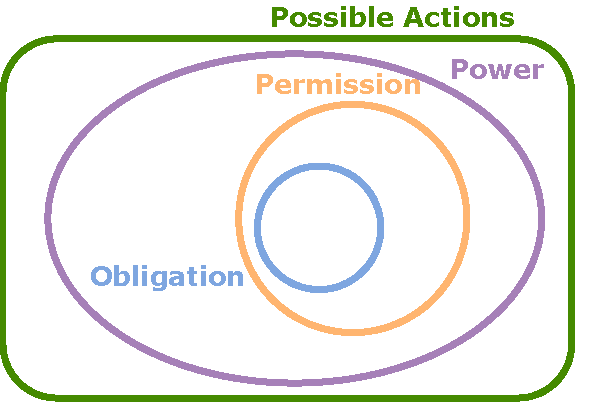
\includegraphics[width=0.6\textwidth]{05_iigo/images/SOMAS_per_obl.pdf}
\caption{Relationship between \emph{power}, \emph{permission} and \emph{obligation}.}
\label{fig:per_obl_sets}
\end{figure} 


For example, the Judge has the \emph{power} to carry out investigations at an IIGO session. There are no rules specifying which specific islands the Judge should investigate. Therefore, the Judge has the \emph{permission} to investigate any `alive' islands during a session. However, the Judge is \emph{obliged} to make at least some number of investigations each turn.



\section{Executive Branch}
\label{sec:executive}
The executive branch is responsible for \textbf{carrying out the law}.
\begin{itemize}
       
    \item The President has the \emph{power} to: 
    \begin{itemize}
        
        \item Select a rule for voting $R^{*}$ to be passed to the Speaker.
        \begin{rule_IIGO}
            The President has the \emph{obligation} to \emph{select} a rule $R^{*}$ if the \emph{rule proposal list} has at least one proposed rule in it.
        \end{rule_IIGO}
        \begin{rule_IIGO}
            The President has the \emph{permission} to \emph{select} a rule $R^{*}$ if and only if $R^{*} \in S$, where $S$ is the \emph{rule proposal list}.
        \end{rule_IIGO}
        
        \item Decide the amount of individual \emph{taxation} (i.e. a specific \emph{minimum} amount of contribution to the common pool for each island) for the current turn.
        
        \begin{itemize}
            \item The President is given the self-reported resource amounts held by each island to assist in this decision.
            %\item Suggested Rule: For any island that has chosen to not report it's resources, the President has the \emph{obligation} to set them an individual tax amount T.
        \end{itemize}
        
        \item Decide the allocation of resources distributed from the common pool to the islands (i.e. a specific \emph{maximum} amount an island is permitted to take from the common pool).
        
        \begin{itemize}
            \item The President is given the \emph{allocation requests} made by each island.
            %\item \emph{}{Suggested Rule:} The President has an obligation to prioritise islands in critical condition.
        \end{itemize}
    \end{itemize}
\end{itemize}



\section{Legislative Branch}
\label{sec:legislative}
The legislative branch is responsible for \textbf{making the law}.
\begin{itemize}

    \item The Speaker has the \emph{power} to:
    \begin{itemize}
        
        \item Call a vote $V$ for a rule $R$.
        \begin{rule_IIGO}
            The Speaker has the \emph{obligation} to \emph{call} a vote $V$ if and only if the President has \emph{selected} a rule $R$ to be voted on.
        \end {rule_IIGO}
        \begin{rule_IIGO}
            The Speaker has the \emph{permission} to \emph{call} a vote $V$ for a rule $R$ if and only if the rule $R = R^{*}$, where $R^{*}$ is the rule \emph{selected} by the President.
        \end {rule_IIGO}
            
        \item Choose which islands are participating in the vote $V$.
       % \footnote{This is our sequential implementation alternative for the power to close the ballot box.}.
        \begin{rule_IIGO}
            The Speaker has the \emph{obligation} to ask for a vote from all alive islands.
        \end {rule_IIGO}
            
        \item Declare the result $C$ of a vote $V$. 
        \begin{rule_IIGO}
            The Speaker has the \emph{obligation} to \emph{declare the result} $C$ for a vote $V$ if and only if the vote V has been \emph{called}.
        \end {rule_IIGO}
        \begin{rule_IIGO}
            The Speaker has the \emph{permission} to \emph{declare the result} $C$ for a vote $V$ if $C = C^{*}$, where $C^{*}$ is the result produced by \emph{calling} the vote $V$.
        \end {rule_IIGO}
        \begin{itemize}
            \item This step is what enables a rule to be \emph{active}.
        \end{itemize}
    \end{itemize}
\end{itemize}




\section{Judicial Branch}
\label{sec:judicial}

The judicial branch is responsible for \textbf{evaluating the law}.
\begin{itemize}
    \item The Judge has the \emph{power} to:
    \begin{itemize}
        \item Perform a number of \emph{inspections}\footnote{An \emph{inspection} \textbf{costs} an expense of resources (See Definition~\ref{def:invst} for more detail).} $I$ and produce a compliance outcome $\mathbb{O}^{*}$\footnote{Note that the compliance outcome $\mathbb{O}^{*}$ considered is a boolean.}.
        %(true: the island has been compliant with the rules in play, false: the island has not been compliant with the rules in play)
        %\begin{itemize}
           % \item For example, to check if the event outcome is \emph{concurrent}\footnote{Again, what is defined as "concurrent"? A clear definition is needed.} with the rules.
        %\end{itemize}
        \begin{rule_IIGO}
            The Judge has the \emph{obligation} to make at least $N$ investigations at each turn.
        \end{rule_IIGO}
        \item Declare the outcome $\mathbb{O}$ of an inspection $I$ to all islands\footnote{This act of broadcasting is especially important for islands to form an opinion about the sanctioned islands accordingly.}.
        \begin{rule_IIGO}
            The Judge has the \emph{obligation} to declare the outcome $\mathbb{O}$ of an inspection $I$ if and only if the inspection $I$ has been performed.
        \end{rule_IIGO}
        \begin{rule_IIGO}
            The Judge has the \emph{permission} to declare the outcome $\mathbb{O}$ of an inspection $I$ if $\mathbb{O} = \mathbb{O}^{*}$, where $\mathbb{O}^{*}$ is the outcome of the inspection $I$.
        \end{rule_IIGO}
        %\item Initiate the removal of the \texttt{President}.
        %\begin{itemize}
            %\item A good Judge would be especially vigilant during \emph{power transfer} regarding the \emph{President} position (see Section~\ref{leg_const} for more detail).
        %\end{itemize}
        \item Invoke economic \textbf{sanctions} (see Section~\ref{sec:sanctions} for more detail).
        \begin{rule_IIGO}
            The Judge has the \emph{obligation} to invoke a sanction $S$ for an island $X$ if and only if an investigation $I$ has an outcome $\mathbb{O}^{*}$ indicating non-compliance, and $I$ is an investigation of an action taken by island $X$.
        \end{rule_IIGO}
        \item Invoke even more severe sanctions in the case of further disobedience to previous sanction(s).
        \begin{rule_IIGO}
            The Judge has the \emph{permission} to invoke a severer sanction $S'$ for an island $X$ if the island $X$ has not fulfilled the requirements of the previous sanction $S$.
        \end{rule_IIGO}
        \item Pardon the islands which are currently sanctioned.
        \begin{rule_IIGO}
            The Judge has the \emph{permission} to revoke any sanction $S$ of an island $X$ at a specific turn.
        \end{rule_IIGO}
    \end{itemize}
\end{itemize}
%(e.g. a new rule that falls under a "sanction" category \hl{[I'm not sure about this being a `new rule` [Ezgi]]}

\subsection{Sanctions}
\label{sec:sanctions}
All sanctions are of economic nature which include:
        \begin{itemize}
            %\item Revoking an island's access to the common pool.
            \item Enforcing an island to contribute a specific amount of resources to the common pool.
            \begin{itemize}
                \item This does not mean that the Judge has the \emph{power} to take resources from an island in order to put them to the common pool -- the island itself is expected to carry out this implication imposed by the sanction itself, otherwise further punishment can be induced by the Judge.
                \item Similarly, \emph{opinion formulation} will follow accordingly whether the island(s) is/are following the implications imposed by the sanction(s).
            \end{itemize}
        
    \end{itemize}
    Sanctions are the associated penalty that comes with an island breaking a specific rule. The Judge is in full control of the penalties associated with breaking any rules. Once the Judge has specified the score of the penalty associated with each time an island breaks a rule, the cumulative penalties accumulated by the island are then used to determine which \textbf{sanction tier} that each island falls into. The score threshold to determine the boundaries of the sanction tiers are set by the Judge. At each turn of the game, each island is told whether they are being sanctioned, and if so, which \textbf{sanction tier} that they are currently in. The \textbf{sanction tiers} of the non-compliant islands are also broadcasted to the other islands in the archipelago. To summarise, the sanctioning process follows these steps:
    
    
    
    %Sanctions are based on an island breaking a rule. Each rule must therefore have an associated penalty. By default, we set these penalties such that they add $1$ to the total sanction score for each island. However, we allow the judge to override this scoring, the judge is able to set their own scores for any particular rule as they desire. This custom scoring is then used when an island breaks a particular rule. By looking at events that occurred in the last turn, and using the customised scoring we provide the holder of the judge role with full control of the penalties for breaking any rules.
    
    





%we then use the cumulative penalties accumulated by each island to determine which Sanction Tier they fall into. The score threshold's required to fall into these sanction tiers is set by the judge and is checked for monotonicity. Each island is told whether they are being sanctioned, and is so what tier they are in. We also tell other islands about which sanction tiers other islands have fallen into. 

    \begin{enumerate}
        \item The Judge has the \emph{power} to set custom penalties associated with breaking any rules.
        \item The Judge is given a list of all events that occurred in the previous turn.
        \item The Judge has the \emph{power} to check whether any, or all of these previous events, involve the islands in the archipelago breaking any rules.
        \item Each of the transgressions is scored using the Judge's custom penalties if the Judge has set them. Otherwise, a score of $1$ is given each time a rule is broken.
        \item The Judge has the \emph{power} to revise the sanction thresholds.
        \item Using the latest sanction thresholds available, each island is assigned to a sanction tier based on the sanction score that it has received.
        \item These sanction tiers are broadcasted to all of the islands in the archipelago.
        \item The Judge then uses sanctions rules in place to calculate the specific amount of resources that each non-compliant island has in order to determine how much it should contribute to the common pool, based on the sanction tier that it is in.
    \end{enumerate}



\section{Constitutional Rights and Obligations in the Archipelago}
\label{sec:const_rights_obl_archi}
Each island has the \emph{power} to:
\begin{itemize}
\item make an \emph{allocation request} (see Definition~\ref{def:alloc_req}) to the President for a specific amount to be allocated to them.
\item report the number of resources it is in possession of to the President.
\begin{rule_IIGO}
    Each island has the \emph{obligation} to report the number of resources it is in possession of to the President.
\end{rule_IIGO}
\begin{rule_IIGO}
    Each island has the \emph{permission} to report the number of resources $R'$ if and only if $R' = R$, where R is the number of resources the island is in possession of.
\end{rule_IIGO}
\item take resources from the common pool.


\begin{rule_IIGO}
    Each island has the \emph{permission} to take at maximum $N$ resources, where $N$ is the specific allocation made by the President to that island\footnote{If no such allocation is made, the island is \emph{permitted} to take any amount of resources.}.
\end{rule_IIGO}
\item contribute resources to the common pool.
\begin{rule_IIGO}
    Each island has the \emph{obligation} to contribute to the common pool an amount greater or equal to that of the individual tax set by the President.
\end{rule_IIGO}
                %The President is in
                %(unless there is a rule in place that dictates how Speaker is to allocate resources).
\item add a rule to the \emph{rule proposal list} (see Definition~\ref{def:rule_prop_list}) at the start of each turn.
        %\begin{itemize}
            %\item The game specification includes how many rules an island can propose each turn.
        %\end{itemize}
        %\item vote  for rules in the Legislative Branch and vote for their favourite islands in elections
\item participate in the legislative branch of the government by casting ballots in votes called by the Speaker
\item vote for an island to be elected for a specific role (e.g. the President, Judge, Speaker) during the elections\footnote{This will be assumed to be true \underline{unless stated otherwise}. %Note that \textbf{diplomatic sanctions} can disable this power of a specific island (see Section~\ref{jud_const}).}.
        }.
\end{itemize}
\section{Accountability Cycle}
\label{sec:accountability}

The IIGO roles (i.e. the President, Speaker and Judge) hold a considerable amount of \emph{power}. To ensure that the government is able to avoid corruption and abuse of power, each branch of IIGO is accountable to another through the accountability cycle. 
The President is accountable to the Speaker, the Speaker is accountable to the Judge, and the Judge is accountable to the President (see Figure~ \ref{fig:cycles_in_IIGO}). This accountability cycle is enacted through \emph{monitoring} actions\footnote{Note that the terms \textbf{monitoring} and \textbf{investigation} have similar but not identical meanings and different consequences in the context of IIGO.}. The desired effect is for any wrong-doing in IIGO to be determined as quickly as possible and the role in question to be replaced. 

The powers related to the accountability cycle and transfer-of-power for each role can be summarized as the following: 
\begin{itemize}
    \item The Speaker has the \emph{power} to: 
    \begin{itemize}
        \item monitor the President.
        \item declare the result of this monitoring and oblige the Judge to initiate power transfer for the President, if the monitoring result indicates wrongdoing.
    \end{itemize}
    \item The President has the \emph{power} to: 
    \begin{itemize}
        \item monitor the Judge.
        \item declare the result of this monitoring and oblige the Speaker to initiate power transfer for the Judge, if the monitoring result indicates wrongdoing.
    \end{itemize}
    \item The Judge has the \emph{power} to: 
    \begin{itemize}
        \item  monitor the Speaker.
        \item declare the result of this monitoring and oblige the President to initiate power transfer for the Speaker, if the monitoring result indicates wrongdoing.
    \end{itemize}
\end{itemize}

%Unlike investigations performed by the Judge, who performs investigations on island actions in the following turn, each role is given the opportunity to check up on the actions of the role it is responsible for immediately after they have been performed. In this sense, the President can monitor (includes investigative-monitoring) the powers (calling a vote and announcing the result) acted on by the Speaker immediately after the Speaker's announcement (or lack there of). The government officials hold a lot of power so this is to ensure that any wrong-doing is determined as quickly as possible. For this project we are only pursuing one degree of monitoring, that is, the powers relating to the accountability cycle will not be monitored themselves. We assume that agents will act in the interest of themselves and keeping all the islands alive is beneficial to everyone. Hence, while the agents might be inclined to break rules in order to benefit themselves, anyone else breaking the rules is seen as undesirable under the assumption that the system in place is there to benefit all. 

The result of monitoring is intended to be a trigger for the initiation of power transfer, whereby a declaration of a negative result indicates that at least one rule was broken by the role monitored and the role should be re-elected. Each turn, in addition to monitoring the actions taken by the role in that IIGO session, the election that role held in the previous IIGO session, if one was held at all, is checked for compliance with the rules of power-transfer.

Figure~ \ref{fig:cycles_in_IIGO} illustrates the reverse nature of the monitoring and power transfer cycles. This is a choice made by design to spread out the process of pre-mature removal from power as a result of wrongdoing. The goal is to avoid malice. If it is one role's power to monitor, it is the other's to initiate and facilitate power transfer. Hence the latter is given a second opinion for cases where the declaration of wrongdoing is not thruthful.

Within the scope of the coursework, we decided to pursue only \emph{one degree of monitoring}, meaning that the powers relating to the accountability cycle will not be monitored themselves. We assume that agents will act in the interest of all the islands in the archipelago. Hence, while the agents might be inclined to break the rules to benefit in some form, it is assumed that the others will negatively see any non-compliant islands based on the assumption that the proposed IIGO system is in place to maintain the welfare of all the islands. We still have rules governing this process (see Rule~\ref{rule:monitoring_1} and Rule~\ref{rule:monitoring_2}), however these rules are not enforced.

The \emph{one degree of monitoring} is another justification for the reverse nature of the monitoring and power transfer cycles. The addition of a second opionion means that a role does not hold the power to both wrongfully declare wrongdoing and hold an election for the same role. 

Let role $X$ be accountable to the role $Y$, which is accountable to the role $Z$. Then:
\begin{rule_IIGO} \label{rule:monitoring_1}
    $Y$ has the \emph{obligation} to declare the outcome of the monitoring result $M$ associated with the action $A$ undertaken by $X$ if and only if $Y$ has monitored the action $A$ performed by $X$. 
\end{rule_IIGO}
\begin{rule_IIGO} \label{rule:monitoring_2}
    $Y$ has the \emph{permission} to declare the monitoring result $M$ associated with the action $A$ undertaken by $X$ if and only if $M = M^{*}$, where $M^{*}$ is the outcome of \emph{monitoring} action $A$ performed by $X$\footnote{These constitutional rules should be available to the agents to check their decisions against. However, due to having only one degree of accountability cycle in place, these rules are not enforced through any sanctions (i.e. breaking these rules has no consequence as they are only deemed to be an \emph{agreement} between the roles).}.
\end{rule_IIGO}


\begin{figure}[!htb]
\centering
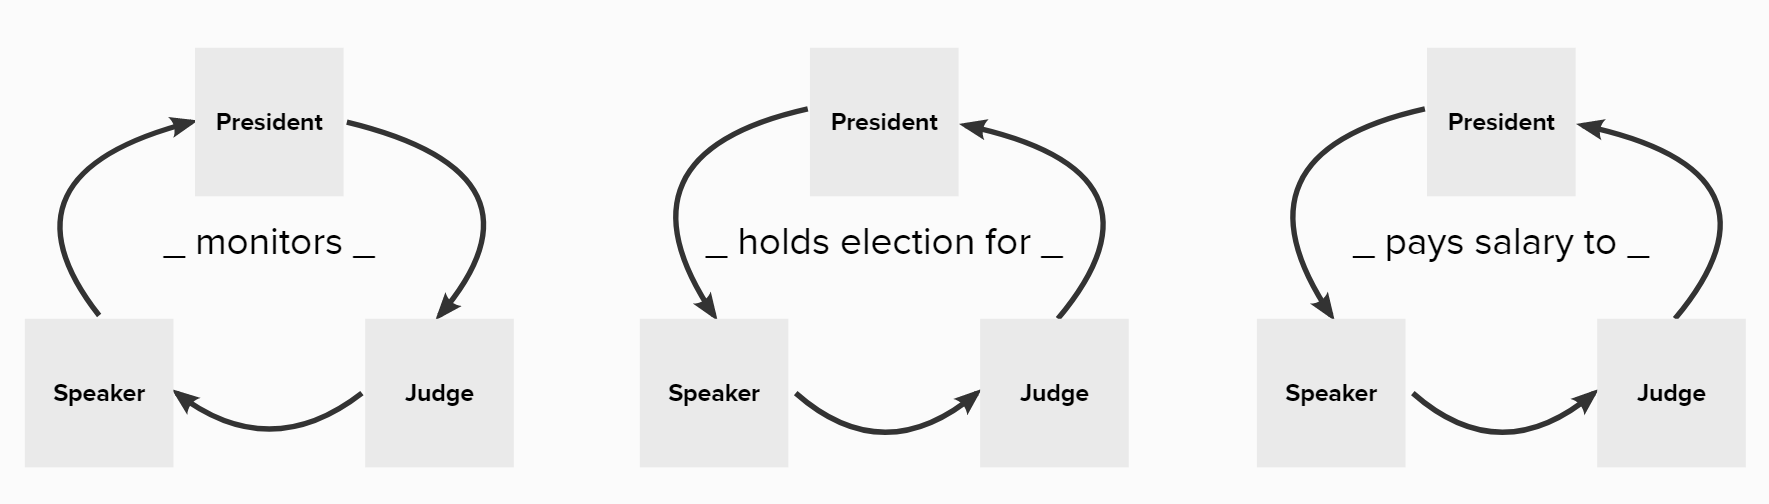
\includegraphics[scale=0.33]{05_iigo/images/role cycles.png}
\caption{Accountability cycle (left), the transfer-of-power cycle (middle) and salary cycle (right).}
\label{fig:cycles_in_IIGO}
\end{figure}


\subsection{Transfer-of-power}
\label{subsec:transfer-of-power}

For the scope of this project, we chose elections to be the only system of power transfer for the islands to utilise. The islands that hold institutional power are the decision group of the archipelago. They decide on taxes, allocations and sanctions. By holding an election for the institutional roles, the islands are not directly included in the decision group, but they do participate in deciding who will occupy these roles and thus who makes the aforementioned decisions. Elections also open up another avenue for opinion formation to have an effect. 
\begin{itemize}
    \item Each role has the \emph{power} to call an election vote and declare the winner (see Figure~ \ref{fig:cycles_in_IIGO} for the power transfer cycle). 
\end{itemize}

We note that:
\begin{enumerate}
    \item The Speaker conducts an election to appoint a new Judge.
    \item The Judge conducts an election to appoint a new President.
    \item The President conducts an election to appoint a new Speaker.
\end{enumerate}
Refer to the Figure~ \ref{fig:cycles_in_IIGO} for further clarification about the transfer-of-power cycle.

We introduce a \emph{term} length to increase the diversity of the decision group. If the Rule~\ref{rule:roles_must_hold_election} is in play, the roles are obliged to hold an election every N turns. To reduce the scope of the coursework, the term length is defined as a configuration parameter. Thus we reduce the complexity of reasoning the agents have to do with reagard to the transfer-of-power of roles.

\begin{rule_IIGO} \label{rule:roles_must_hold_election}
    The role $X$ has the \emph{obligation} to conduct a vote for the election of $Y$ if and only if $Y$ has been in power for more turns than the turn length or if role $Z$ has made a monitoring anbnouncement that indicates wrongdoing by $Y$
\end{rule_IIGO}

\begin{rule_IIGO} \label{rule:must_appoint_elected_island}
    The role $X$ has the \emph{permission} to \emph{declare the winner} $W$ for an election $E$ if $W = W^{*}$, where $W^{*}$ is the winner produced by \emph{calling} a vote for the election $E$.
\end {rule_IIGO}

Unlike the speaker, the process of election is more regimented. The power of calling a vote for an election and the power of declaring the result are combined into one action. The decision came as a result of motion to simplify the system for implementation. However, the powers are still, somewhat, kept seperate. When facilitationg an election the roles still have the option to declare a winner of their choosing. Rule~\ref{rule:must_appoint_elected_island} is what governs this choice. The agents don't, however, have the option to not declare a result at all, holding an election will always result in an declaration of the winner. 

\section{Budget and Salary}
\subsection{Budget}
%Actions associated with the IIGO have an associated cost that is defined as a configuration parameter. The institutional-power-enabled actions of  identified to require a "computational" component are:

For the simulation we have defined the resources gathered by the islands to be endogenous. Hence we assume that self-organisation will consume those resources and institutional-power actions in the IIGO have an associated cost. The institutional-power actions with such a cost are:


%that is defined as a configuration parameter. The institutional-power-enabled actions of  identified to require a "computational" component are:


%We have defined the resource to be an endogenous one, hence any computation surrounding the distribution of the resource must use up some of that resource. 
\begin{itemize}
\item President: Selecting a rule from the rule proposal list.
\item President: Deciding the amount of individual taxation.
\item President: Deciding the allocation of resources from the common pool.
\item Speaker: Calling a vote and calculating the winner.
\item Judge: Inspecting an island's actions.
\item Judge: Inspecting an island's action history retroactively.
\item Declaring (e.g. \textit{announcing} the result of a vote).
\item Holding an election.
\item Monitoring a role.
\end{itemize}

IIGO has been designed to act in the common good. Therefore IIGO-related costs will be directly withdrawn from the common pool. Since the common pool is considered communal property of the archipelago, there are rules in place to limit how much each role is allowed to spend in order to perform its own institutional-power-enabled actions. This is the reason for defining the \emph{budget} and keeping it separate for each of the three IIGO roles.

\begin{rule_IIGO} \label{rule:budget}
    %Each role has the \emph{obligation} to pay the salary of amount $S$ to another if and only if the amount paid $S'$ is equal to $S$.
    Each role has the \emph{permission} to act on an institutional-power action with an associated cost if the budget would not become negative as a result of performing the action.
 \end{rule_IIGO}



When a role acts on an institutional-power action with a cost, the cost associated with this action is subtracted from the role's \emph{budget}. If Rule~\ref{rule:budget} is in play, a budget of zero or less means that the role does not have the \emph{permission} to perform any of its institutional-power actions. The removal of Rule~\ref{rule:budget} from the rules in play means the role is permitted to perform as many such actions as it would like (as long as those actions are not governed by other rules). 

The \emph{budget} is persistent across turns. This means that, assuming nothing else affects the budget, if a role has $100$ resources in its budget at the start of a turn and spends $10$ resources, the same role has $90$ resources in its budget at the start of next turn. On the other hand, islands can choose to increase the budget periodically every turn. The islands can choose the magnitude of this periodic increase by voting on a rule.

%one turn and it spends 10, it has 90 resources in it's budget the next turn. 

Finally, it must be noted that the budget is inherently linked with  whether the obligations of a specific role can be undertaken.
For example, during \emph{monitoring}, it is not seen to be a rule violation if a role has not acted on an obligation as doing so would require it to go over budget.

%This can also be seen as an added clause "... and the action is only permitted if they have the budget" to most rules which govern actions with an endogenous-cost.
%\begin{rule_IIGO}
    %The budget is increased by an amount $N$ every turn.
%\end{rule_IIGO}

%This rule means that, assuming nothing else affects the budget, if a budget is set to increase by 10 resources every turn and the budget is a 100 resources in turn one, the budget is 110 resources in turn 2. Setting this rule to 0 is equal to removing this rule and it means that the budget is never increased. 


\subsection{Salary}
\label{subsec:salary}
A salary is paid to each role in power as an incentive to be in power. Since our system has regimented the means of power transfer to be an election, this incentive extends to acting in a publicly approved way. %Hence, each role has the \emph{power} to pay a salary to another role following the salary cycle in Figure~\ref{fig:cycles_in_IIGO}.
\begin{rule_IIGO} \label{rule:salary}
   Each role has the \emph{obligation} to pay the salary of amount $S$ to one another following the salary cycle in Figure~\ref{fig:cycles_in_IIGO}.
\end{rule_IIGO}

In Rule~\ref{rule:salary}, setting $S=0$ (through changing the active rules in place) means that roles do not have the permission to pay any salary. Removing the Rule~\ref{rule:salary} means that the roles may freely choose the amount $S$ for the salary payments.

\section{IIGO Session Order}
Each IIGO Session can be broken down into a sequence of consecutive actions by the Judiciary, Executive and Legislature. The session is concluded with monitoring, salary payments and elections.
\subsection{Judicial Actions}
\begin{enumerate}
    \item The Judge has the \emph{power} to check the history of actions to confirm whether the previously punished island(s) has/have obeyed the previous round's sanctions, meaning whether they contributed to the common pool accordingly in case of economic sanctions.
    %\begin{itemize}
      %  \item \emph{Suggested Rule:} In case of disobeying sanctions, the Judge is \emph{obliged} and \emph{permitted} to increase the severity of sanctions with respect to specific islands.
   % \end{itemize}
    \item The Judge has the \emph{power} to carry out \emph{inspections} on the history of actions of any island $X$ to check whether:
        \begin{enumerate}
        \item the reported resources of $X$ in the previous round match the real value of resources $X$ had in its private pool for the previous turn.
        \item the island $X$ has retrieved the right amount of the resources from the common pool, based on the \emph{allocation request} evaluated by the previous President.
            \begin{itemize}
            \item An example: In the previous round, the President has decided that the island $X$ can take $Y$ amount of resources from the common pool. If the Judge finds out that the island $X$ has taken an amount of $Y'$ such that $Y' > Y$, the Judge has the \emph{power} to invoke sanctions on the island $X$.
            
            %the Judge is \emph{obliged} and \emph{permitted} to sanction island $X$.
            \end{itemize}
        \end{enumerate}
    \item The Judge has the \emph{power} to invoke sanctions based on the outcome of the inspections.
\end{enumerate}
\subsection{Executive Actions}
\begin{enumerate}
    \item The islands may report the resources in their private pools to the President.
    \item The President has the \emph{power} to let each island know about the amount of \emph{taxation} they have to pay.
    \item The island has the \emph{power} to make an \emph{allocation request} to the President.
    \item The President has the \emph{power} decide on an allocation of resources and let each island know about the amount of resource allocation they are permitted to take from the common pool.
    \item The island has the \emph{power} to pick and to propose a rule to be voted on to the President.
    \item The President has the \emph{power} to choose a rule to be voted on from the received rule proposals.
\end{enumerate}
\subsection{Legislative Actions}
\begin{enumerate}
    \item The Speaker has the \emph{power} to call a vote.
        \begin{enumerate}
        \item The islands vote in support of, or against, the rule (aye or nay) anonymously.
        \end{enumerate}
    \item The Speaker has the \emph{power} to announce a result of a vote to the islands and carries out the law change, if required (e.g. deleting/rejecting a rule if there is a majority nay vote).
\end{enumerate}
\subsection{End of Session Actions}
\begin{enumerate}
    \item The roles pay a salary to one another following the accountability cycle in Figure~ \ref{fig:cycles_in_IIGO}.
    \item The Speaker has the \emph{power} to decide to carry out \emph{monitoring} on: 
    \begin{enumerate}
    \item the resource allocation decided by the President.
    \item the rule proposed by the President.
    \item the previous IIGO session's election for a new Speaker, if an election was held.
    \end{enumerate}
    \item The President has the \emph{power} to decide to carry out \emph{monitoring} on:
    \begin{enumerate}
        \item the sanctions imposed by the Judge.
        \item the previous IIGO session's election for a new President, if an election was held.
    \end{enumerate}
    \item The Judge has the \emph{power} to decide to carry out \emph{monitoring} on:
    \begin{enumerate}
        \item the vote called by the Speaker.
        \item the Speaker announcing the result.
        \item the previous IIGO session's election for a new Judge, if an election was held.
    \end{enumerate}
    \item The Speaker has the \emph{power} to decide to hold an election for a new Judge.
    \item The President has the \emph{power} to decide to hold an election for a new Speaker.
    \item The Judge has the \emph{power} to decide to hold an election for a new President.
\end{enumerate}



\section{Future Work}

\begin{itemize}
    \item \textbf{Diplomatic sanctions}: Although having the potential of being a good alternative for severer sanctions discussed in  Section~\ref{sec:sanctions}, diplomatic sanctions are \emph{not} implemented within the scope of the coursework. \\
    Suggested diplomatic sanctions include:
        \begin{itemize}
            \item Revoking an island's eligibility to vote and to be elected for a position.
            \item Revoking an island's eligibility to propose a rule/motion.
        \end{itemize}
    \item \textbf{Immutable rules}: Within the scope of the coursework, a subset of rules could have been categorised as immutable. This means that to change such immutable rules, the islands first need to vote to change their status to be \emph{mutable}, and consequently, hold another vote to change these mutable rules.
    %\item \textbf{Adding rules to the proposal list: } 
\end{itemize}

    \chapter{Voting}
\section{Voting Scenarios}
\label{sec:VotingScenarios}

The voting is called when a collective decision is needed to make in a justified way. A robust voting system is designed for the organisational meetings especially for IIGO in this coursework. % TODO ref to IIGO chapter
When a voting is called in IIGO, the roles President, Speaker, Judge, and Voters will be empowered to have relevant functions to proceed a series of action:
\begin{itemize}
    \item President will be eligible to select a motion for the archipelago to vote for.
    \item Speaker will be eligible to take charge of the proceeding of voting i.e. receiving ballots, counting ballots, and declare the winner.
    \item Judge will be eligible to inspect ballots and the Speaker's action. % ref to IIGO judge inspectBallot
    \item Voters will be eligible to vote i.e. submit ballots.
\end{itemize}

In an IIGO meeting, the elections of roles and changes of rules need voting for such collective decision-making.

\textbf{Elections of roles:} As per the IIGO specification, the elections of roles will be conducted according to the cycle of accountability i.e. the Judge can initiate the power transfer of the role of President through voting; the President can initiate the power transfer of the role of \texttt{Speaker} through voting; the Speaker can initiate the power transfer of the role of Judge through voting. To prevent multiple-role enactment of one island, the island that has been selected as a role will be removed from the candidates in the voting for other roles in the current turn. Depending on the sequence of the elections called, the candidates for three roles will consist of maximally six, five, and four islands accordingly. The ballots from the Voter islands will be in the format of preference lists, which rank all candidates in an order.

\textbf{Changes of rules:} the President can select a rule from the proposed list to be voted by the Voter islands. The Speaker will host the voting for changes of rules and be responsible for the ballots counting and results declaration. The ballots from the Voter islands will be: Aye, namely agree with the rule change; Nay, namely disagree with the rule change; or Abstain.


\section{Voting Methods}
\label{sec:VotingMethods}

Table \ref{table:votingmethod} indicates available choices for each voting scenario.

\begin{table}[H]
\caption{Available voting methods for each voting scenario}\label{table:votingmethod}
\begin{center}
\begin{tabular}{ |p{3cm}||p{3cm}|p{3cm}|  }
 \hline
 Voting Methods   & Elections of Roles & Changes of Rules   \\
 \hline
 Plurality   &     & \checkmark     \\
 \hline
 Borda Count &  \checkmark   &      \\
 \hline
 Runoff      &  \checkmark    &        \\
 \hline
 Instant Runoff    & \checkmark  &     \\
 \hline
 Approval  &  \checkmark    &    \\
 
 \hline
\end{tabular}    
\end{center}
\end{table}

\textbf{Plurality} will select the majority choices as the collective decision. When the decision is picking between two options, e.g. whether agree or disagree a change of rule. Unlike the elections, it is not necessary to compare the options left for determining a relative preference. It is straightforward and effective especially when the number of valid ballots (i.e. abstention excluded) is odd. However, it requires consideration when the results are tied. The solution to tied results is regimented with the assumption that the proposer of the voting in such events will vote for "agree". Thus, the proposal will be approved if the number of "agree" votes is more than the number of "disagree" votes. 

\textbf{Borda Count} method will allow voters to rank preference instead of choosing one option only. The order of choices in the preference list determines the Borda points regarding each option. Adding such Borda points from all voters' ballots produces the Borda score for each candidate. Thus, the candidate with the highest Borda score will be the collective decision.

% The tied results are resolved by selecting the most first-nominated candidate. If this still gives multiple winners, the most second-nominated candidate will be selected as the winner. This iterative counting process will act as a tiebreaker for winner selection.

\textbf{Runoff} (also known as the two-round system) is a voting method which is used to pick a single winner from a list of several candidates. 
%Normally, voters cast a single vote for their preferred candidate, but in our game specification it is also possible for voters to make their preference list.
Runoff voting is widely recognized and used around the world primarily for the election of the head of state. It is an effective voting method for the selection of candidates.

\texttt{Voter} islands will rank their preference of candidates and submit the preference lists as their ballots. In the first round, two candidates with most first placed votes are chosen among all candidates. The Runoff voting can conclude the election in the first-round if one candidate obtains a majority. Otherwise, the second round need to be considered and utilized where the ballots will be recounted by eliminating the candidates other than the top-two. Subsequently, the candidate with the most votes between the top-two candidates will be the winner.

\textbf{Instant Runoff} is a voting method which is used in single-seat elections which consist of more than two candidates. 
Individual voters rank their preference of candidates. The candidate who gets the least number of first-placed is eliminated and this step is repeated until only one candidate remains.

% In the event of tied result, alternative rules can be chosen to give a single winner. It is obvious that the effectiveness of this method comes from its flexibility of various rules available in a tie situation.

\textbf{Approval} is a voting method for single winner in which each voter selects a subset of candidates. As of its procedures and usage in the game, Approval will be used for the elections of roles where each voter picks a group of candidates and the most named or approved candidate wins.

\textbf{Tied situation:} In a tied situation, there are three possible rules that can be used to eliminate one or more candidates who get the same number of votes. The Condorcet method is one of the voting methods which selects the candidate that dominates other candidates in term of majority relation which ranks the candidates according to one-to-one comparisons. In other words, the Condorcet winner is the candidate that wins a majority in every one-to-one comparison against other candidates. However, Condorcet method is not guaranteed to work when preference lists form a cycle, which is known as the Condorcet paradox or voting paradox. Alternatively, Hare Rule can be used in a tiebreak where all candidates with the least first-place votes will be all eliminated. Moreover, Coombs Rule could be used in place of Hare Rule if the iterative process of removing candidates with the least first-place votes is not preferred. Coombs Rule indicates that the candidate with the most last-placed votes will be removed.

In this coursework, the pairwise Condorcet winner is chosen for a tiebreak setup which states that a candidate who dominates the other candidate in term of majority relation wins.

% Whereas the Hare rule removes all candidates with the least first-place votes and Coombs Rule iteratively removes a candidate with most last placed votes.

% Interestingly, Instant Runoff method is criticized by Condorcet for its disadvantage which involves removing a candidate who is favored by a majority of voters.

\section{Voting Protocol}
\label{sec:VotingProtocol}
Voting Protocol is adopted from an example of formal specification given in Robert's Rules of Order (RONR) that defines a series of sequential actions when a voting event happens. This protocol is applicable to any voting method at certain state of the game (i.e. during IIGO session) whenever a voting event happens. With the basis from RONR\footnote{refer to Prof. J Pitt's Draft Book: Self-Organising Multi-Agent Systems (2020) Chapter 4 "Social Choice Theory", Section 4.6.1 Page 114}, the sequence of actions of voting protocol in this game when a voting event happens is as follows (taken an example of voting event for change of rules): the President selects a rule from the rule proposal list to be voted on; the President notifies the Speaker to hold a voting event for the selected rule; the Speaker calls for a vote for the selected rule by opening ballots to all islands to cast their votes; the Speaker closes the ballots after receiving votes from all islands; the Speaker counts the votes by calling an applicable voting method function for winner selection to produce a result; and finally the Speaker publicly declares the voting result whether the selected rule can be carried out or not. Figure~\ref{fig:RONRVotingProtocol} shows the general sequence of the voting protocol for rules.

\begin{figure}[H]
\begin{center}
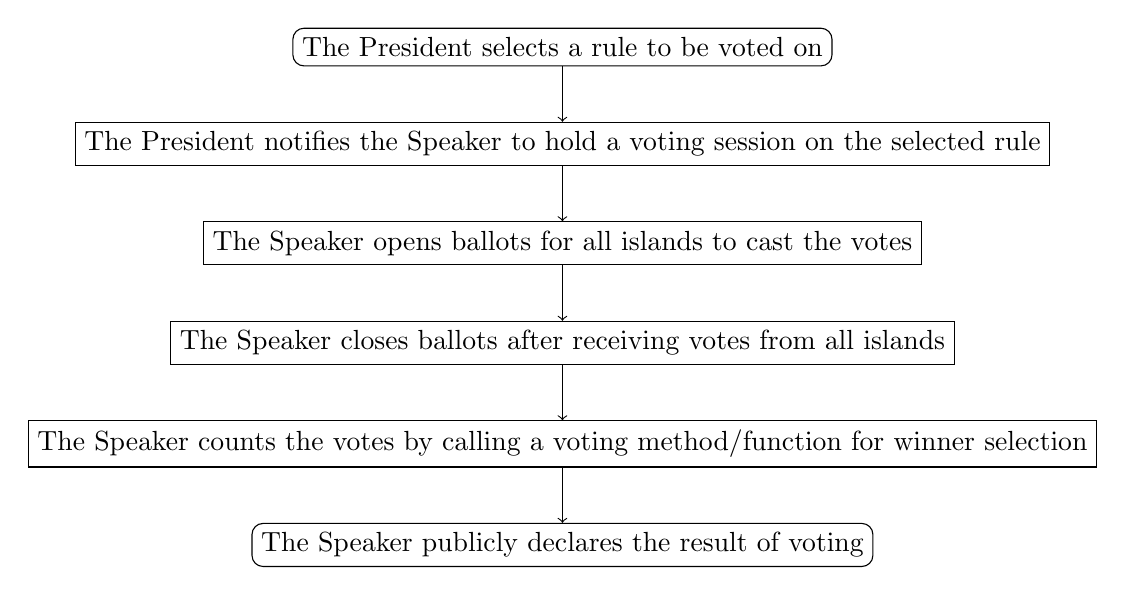
\begin{tikzpicture}[node distance=20pt]
\centering
\node[draw, rounded corners] (start)  {The President selects a rule to be voted on};
\node[draw, below=of start] (step 1)  {The President notifies the Speaker to hold a voting session on the selected rule};
\node[draw, below=of step 1] (step 2)  {The Speaker opens ballots for all islands to cast the votes};
\node[draw, below=of step 2] (step 3)  {The Speaker closes ballots after receiving votes from all islands};
\node[draw, below=of step 3] (step 4)  {The Speaker counts the votes by calling a voting method/function for winner selection};
\node[draw, below=of step 4, rounded corners] (end)   {The Speaker publicly declares the result of voting};
 \draw[->] (start)  -- (step 1);
 \draw[->] (step 1) -- (step 2);
 \draw[->] (step 2) -- (step 3);
 \draw[->] (step 3) -- (step 4);
 \draw[->] (step 4) -- (end);
\end{tikzpicture}
\caption{Voting Protocol for Rules}
\label{fig:RONRVotingProtocol}
\end{center}
\end{figure}

For elections of roles, the sequence of actions of the voting protocol is mostly similar to the above explanation in principle, except for some parameters, such as the motion of the vote which is the role itself (President, or Speaker, or Judge), the facilitator of the election/vote event which depends on what role is being held for election (refer to Chapter 5 IIGO for more details on change of roles and power transfer), and the applicable voting method function to call for election that will produce the result, which is different from the voting method used for rules. Refer to Section~\ref{sec:VotingMethods} for more details on voting methods to be used for elections of roles.

In the initial implementation, it is assumed that all 6 islands have the power to vote at any necessary voting scenario and no sanction or power restriction applied to any island when it comes to the right to vote. However, in the final implementation, some complications or dilemma are applied to, i.e. an/some island(s) could lose their right to vote or not permitted to participate in a voting event due to diplomatic sanction. Refer to Chapter 5 IIGO for details on diplomatic sanction. In this case, the Speaker will check and open the ballots to only eligible islands that have the right to vote at that certain stage, rather than to all islands as mentioned in the first scenario above.

\section{Implementation}
\label{sec:Implementation}

\subsection{Voting for Rules}
\label{sec:VotingForRules}
The implementation of voting for rules from infrastructure point of view (file:\texttt{rulevote.go}) basically follows the sequence of voting protocol as described in Section~\ref{sec:VotingProtocol}. At initialisation, there are two defined structs (collection of data fields) that are used as parameters for functions inside the voting algorithm, such as \texttt{RuleVote} and \texttt{BallotBox}. The \texttt{RuleVote} struct consists of 3 variables, i.e. \texttt{ruleToVote} (string) that contains the rule that has been selected by the President to be voted on, \texttt{islandsToVote} (list of integers) that contains a list of \texttt{ClientID} which indicates all eligible islands that participate in the voting session, and \texttt{ballots} (list of boolean) that contains the vote of each respective eligible islands where it can indicate the vote for in-favour or against the proposed rule. The \texttt{BallotBox} struct consists of 2 integer variables that act as accumulators for the count of each possible vote: \texttt{VotesInFavour} and \texttt{VotesAgainst}.

According to Section~\ref{sec:VotingProtocol}, The Speaker firstly starts a voting session by calling \texttt{SetRule(rule)} function that contains the rule selected by The President to be voted on. Next, the Speaker sets all eligible islands that can participate/have the right to vote in the voting session at that state of the game by using \texttt{SetVotingIslands(clientIDs[])} function. After that, the Speaker opens the ballots to get the votes from all eligible islands by calling \texttt{GatherBallots(clientMap[ClientID])} function. Subsequently, the \texttt{GetBallotBox()} function is called by the Speaker to gather the ballots that already contain the votes counting of those who are in-favour or against the proposed rule. Finally, the votes counting is concluded by comparing the votes of those in-favour vs those against, and the in-favour votes win when the counting is greater than or equal to the against votes counting, as reflected in \texttt{CountVotesMajority()} function. The Speaker then uses this result to declare the result of this voting session in IIGO.

\subsection{Elections}
\label{subsec:Elections}
The elections for roles implementation can be seen in the file:\texttt{election.go}. At initialisation, there is a defined struct \texttt{Election} that contains 4 parameters, i.e. \texttt{roleToElect} that indicates which role is being voted on (President, or Speaker, or Judge), \texttt{votingMethod} that indicates the voting method being used for the election to determine the winner selection, \texttt{islandsToVote} that contains a list of \texttt{ClientID} which indicates all eligible islands that participate in the voting session, and \texttt{votes} that is a list that contains the order rank of preference of the candidates for the role from each eligible island who casts the vote.

The election session begins by calling the \texttt{ProposeElection(role,method)} function that depends on which role being voted on and which role has obligation to facilitate the election (refer to Chapter 5 IIGO on Change of Roles and Power Transfer sections), and the selected voting method to be used for this election (refer to Section~\ref{sec:VotingMethods} for details on voting methods and Subsection~\ref{subsec:VotingPseudo} for pseudo-code implementation). The election facilitator then opens ballots to all eligible islands to cast their votes by calling \texttt{OpenBallot(clientIDs[])} function. The \texttt{Vote(clientMap[ClientID])} function gathers all the ballots containing the votes from all eligible islands that are obtained from \texttt{GetVoteForElection(roleToElect)} function returned from each client/island code execution. After that, the election facilitator closes the ballots by using \texttt{CloseBallot()} function and it returns the result of the votes counting using the selected voting method by calling each respective voting method function. This result is used by the election facilitator to declare the winner for the elected role. By default, the voting method for election is Borda Count and the function is called \texttt{bordaCountResult()} where the algorithm follows through what are explained in Section~\ref{sec:VotingMethods} and Subsection~\ref{subsec:VotingPseudo} where the Borda scores will be calculated based on the order rank of preference of the candidates from each ballot. The other voting methods can be used for election and it is selected by the election facilitator.

\subsection{Voting Methods Implementation Pseudo-code}
\label{subsec:VotingPseudo}

\textbf{Plurality}
\newline
Call for Voting inputs (int:IslandID, str:"Aye", "Nay" or "Abstain")\\
\begin{algorithm}[H]
\ForEach{$ballot \in ballots $}{
    \If{$Aye$} {Count for $Aye ++ $}
    \If{$Nay$} {Count for $Nay ++ $}
}
\If{$Aye > Nay$}{\Return the Winner: $Aye$}
\Else{\Return the Winner: $Nay$}
\end{algorithm}

\ \newline \ \newline \ \newline
\textbf{Borda Count}
\newline
\begin{algorithm}[H]
\For{all ballot}{
    $numNotIn\gets N-ballot.length$\\
    $shareScore\gets 1+...+numNotIn$\\
    \For{i from 0 to N-1}{
    \If{i is in ballots} {$scores[i]\gets scores[i]+N-K+1$ }
    \Else {$scores[i]\gets scores[i]+shareScore/numsNotIn$ }
    }
}
Sort candidates by Borda scores\\
\Return the candidate with the highest score
\end{algorithm}

\ \newline \ \newline \ \newline
\textbf{Runoff}
\newline
\begin{algorithm}[H]
\For{All $ballot \in ballots $}{
    Select two candidates with most first-placed votes
}
\If{either already has a majority}{
\Return the majority one}
\Else{Each voter selects one candidate of the top 2\\
}
\Return the candidate with the most votes
\end{algorithm}

\ \newline \ \newline \ \newline
\textbf{Instant Runoff}
\newline
\begin{algorithm}[H]
\ForEach{$ballot \in ballots $}{
\For{i from 0 to N-1}{
\If{i is first choice}{$scores[i]\gets scores[i]+N-K+1$}
}
}
\If{candidate in ballots $>1$}{
Remove the candidate with the fewest first
choice votes from the ballots.\\
GOTO the top for next round of counting
}
\Else{\Return the candidate}
\end{algorithm} 

\ \newline \ \newline \ \newline
\textbf{Approval}\\
\begin{algorithm}[H]
\ForEach{$ballot \in ballots $}{
    \For{i from 0 to N-1}{
    \If{i is in ballot} {$scores[i]\gets scores[i]+1$ }
    }

}
Sort candidates by scores\\
\Return the candidate with highest score
\end{algorithm}

    \chapter{Team 1 Agent Design}

\section{Core Idea}
Team 1 Agent was designed around the idea that the agent wants the whole archipelago to survive. However, the agent does have different configurations that allows it to be more malicious than intended such that interesting simulations may occur.

\section{Opinions on Islands}
For an agent to become self-organising, the agent must determine certain actions given a condition without external input. For this to be possible, the agent must have defined conditions which team 1 calls 'emotional state', and hold an opinion about other islands. This will form a basis for the agent to decide on an action.

Initially, the opinion on all existing islands are neutral. Overtime through IITO and IIGO, the opinions on islands will change. This will affect the outcome of IITO and IIGO results. As a note, positive values correspond to positive opinions while negative values correspond to negative opinions.

An agent's emotional state can change depending on the current resources. Below is an example of how an agent's emotional state can be formed:
\begin{itemize}
    \item If current resources > 10 * living cost, the agent is happy.
    \item If 3 * living cost < current resources < 10 * living cost, the agent is anxious.
    \item If the current resources < 3 * living cost, the agent is desperate.
\end{itemize}
The upper and lower bounds can be changed before a game starts. 

\section{IITO Gifts}
During IITO, the agent's opinion of other island is affected. For every gift received, the agent's opinion of the gifter increases. However, the agent's opinion of an island can decrease if that island promised a gift and was not able to fulfil it. 

When team 1 agent receives a request for gifts, the agent will decide how much to offer depending on the agent's current emotional state and the opinion of that island. 

\begin{table} [htb]
    \centering
    \begin{tabular}{|c|p{0.5\textwidth}|}
        \hline
        Emotional State & How is IITO handled? \\
        \hline
        Happy & Agent will give away its resources that satisfies the requested amount. \\
        \hline
        Anxious & Agent will give away a ratio of the requested amount and its current resources. \\
        \hline
        Desperate & Agent will refuse any gift requests that it receives. \\ 
        \hline
    \end{tabular}
\end{table}

Moreover, if the agent's opinion of an island is very high, the agent can decide to give gifts disregarding the agent's own anxiety. On the other hand, if an opinion of an island is very low, the agent can decide to refuse to send a gift even though the agent is happy. 

For increase survivability, team 1 agent will accept any gift offers that it receives. 

\subsection{Future Works}
Team 1 agent currently has a very straight-forward IITO strategy. Some interesting alteration to this strategy could include:
\begin{itemize}
    \item Being less suspectible to bribery. The agent should stop increasing the opinion of an island after receiving $X$ amount of continuous gifts.
    \item Stop handing out gifts to islands that are not in critical state.
    \item Being proactive in bribery. The agent will give unrequested gifts to the current president in hopes that this will reduce tax and increase resource allocation from the common pool. 
\end{itemize}

\section{IIFO Disaster Prediction}
Disasters can happen deterministically or stochastically (mentioned in detail in Chapter~\ref{sec: Disaster} for more information). For an agent, it is important to determine when a disaster occurs so that as much disaster damage is mitigated using the common pool. 

When the game starts, the disaster prediction made by the agent is random. This prediction always has a confidence value of 0. As more disasters occur, a history of disasters is built up. Using this history, the mean disaster position x, position y, magnitude and occurrence is calculated. A confidence value is calculated along with the mean disaster metrics. 

% Add a footnote on website?  https://www.mathsisfun.com/data/confidence-interval.html
The confidence value is calculated by finding the ratio between margin of error and the mean value. The smaller the margin of error, the more confident the agent is. Therefore, a difference between the mean value and the margin of error must also be calculated. To begin with, the agent uses the confidence interval equation (where $s =$ standard deviation, $n = $ size of array, $Z = $ confidence interval) to calculate the margin of error:
\begin{equation}
    \label{eq: Team1MarginOfError}
    \text{Error} = Z \dfrac{s}{\sqrt{n}} 
\end{equation}
Using the difference between the mean value ($\bar{x}$) and the margin of error along with finding out the ratio of this result will provide the agent with the confidence value.
\begin{equation}
    \text{Confidence Value} = (\bar{x} - \text{Error}) \times \dfrac{1}{\bar{x}}
\end{equation}

Sharing and obtaining other disaster information to and from other islands respectively can increase the survivability of the archipelago. As more disaster prediction is shared, a network of trust between team 1 agent and other island is built. This trust value is primarily based upon the absolute value of the islands prediction on the day the disaster happened. However, if an island shares a disaster prediction with the estimated disaster day to be random or changing erratically each turn, then team 1 agent will begin to distrust that island. 

\section{IIGO: President}

\section{Foraging}
Multiple foraging strategies were developed: 
\begin{itemize}
    \item Return on Investment (ROI)
    \item Regression
    \item Flip Forage
\end{itemize}

\subsection{Simulations against ourselves}

Multiple foraging strategies were developed, initially by intuition and later by attempting to address the shortcomings of previous attempts:

\subsection{Return on Investment (ROI) Foraging}%
\label{sec:forage-roi}

This first algorithm is based on repeating successful foraging behaviours in the past, whether those be by the agent herself or another agent.

For the first few turns (the exact amount is configurable) the agent will forage randomly.

The agent maintains a history of foraging decisions and outcomes, including those received from IIFO.\@ When it comes time to forage this history is sorted by ROI, i.e.\ the ratio of profit to contribution. Decisions that resulted in a loss, had profit smaller that the living cost, or had a larger contribution that a (configurable) percentage of available resources are filtered out.

\subsection{Regression Foraging}%
\label{sec:forage-regression}

This strategy tries to predict the ideal foraging decision, even if that exact decision was not made in the past. This is done using regression, which is used to find the decision with the highest expected reward.

% In detail, history is kept as in \nameref{sec:forage-roi}. To make a foraging decision, the history is split by foraged resource (fish or deer), and quadratic regression is performed on contribution versus reward. The maximum of the regression curve is found for each group and the contribution with the highest

\subsection{Flip Foraging}

This strategy chooses the least foraged resource from the last turn, according to IIFO-reported data. Contributed amount is proportional to the chosen resource's total ROI from last turn. This choice was made under the assumption that ROI is an indicator of the resource's ``condition''. If a resource only gives moderate rewards (proportionally to input) it means that it is probably over-used currently and as such agents should allow it to recover, by scaling down their foraging attempts.

\subsection{Comparison}

To compare the three strategies, simulations were run with six agents, two using \emph{ROI foraging}, two using \emph{regression foraging}, and two using \emph{flip foraging}. IIGO and IITO were also disabled in order to isolate the efficacy of foraging methods from other parts of the game. The simulation was run five times and the results averaged over the 5 games as well as the two agents following the same strategy.

\begin{figure}[H] 
\centering
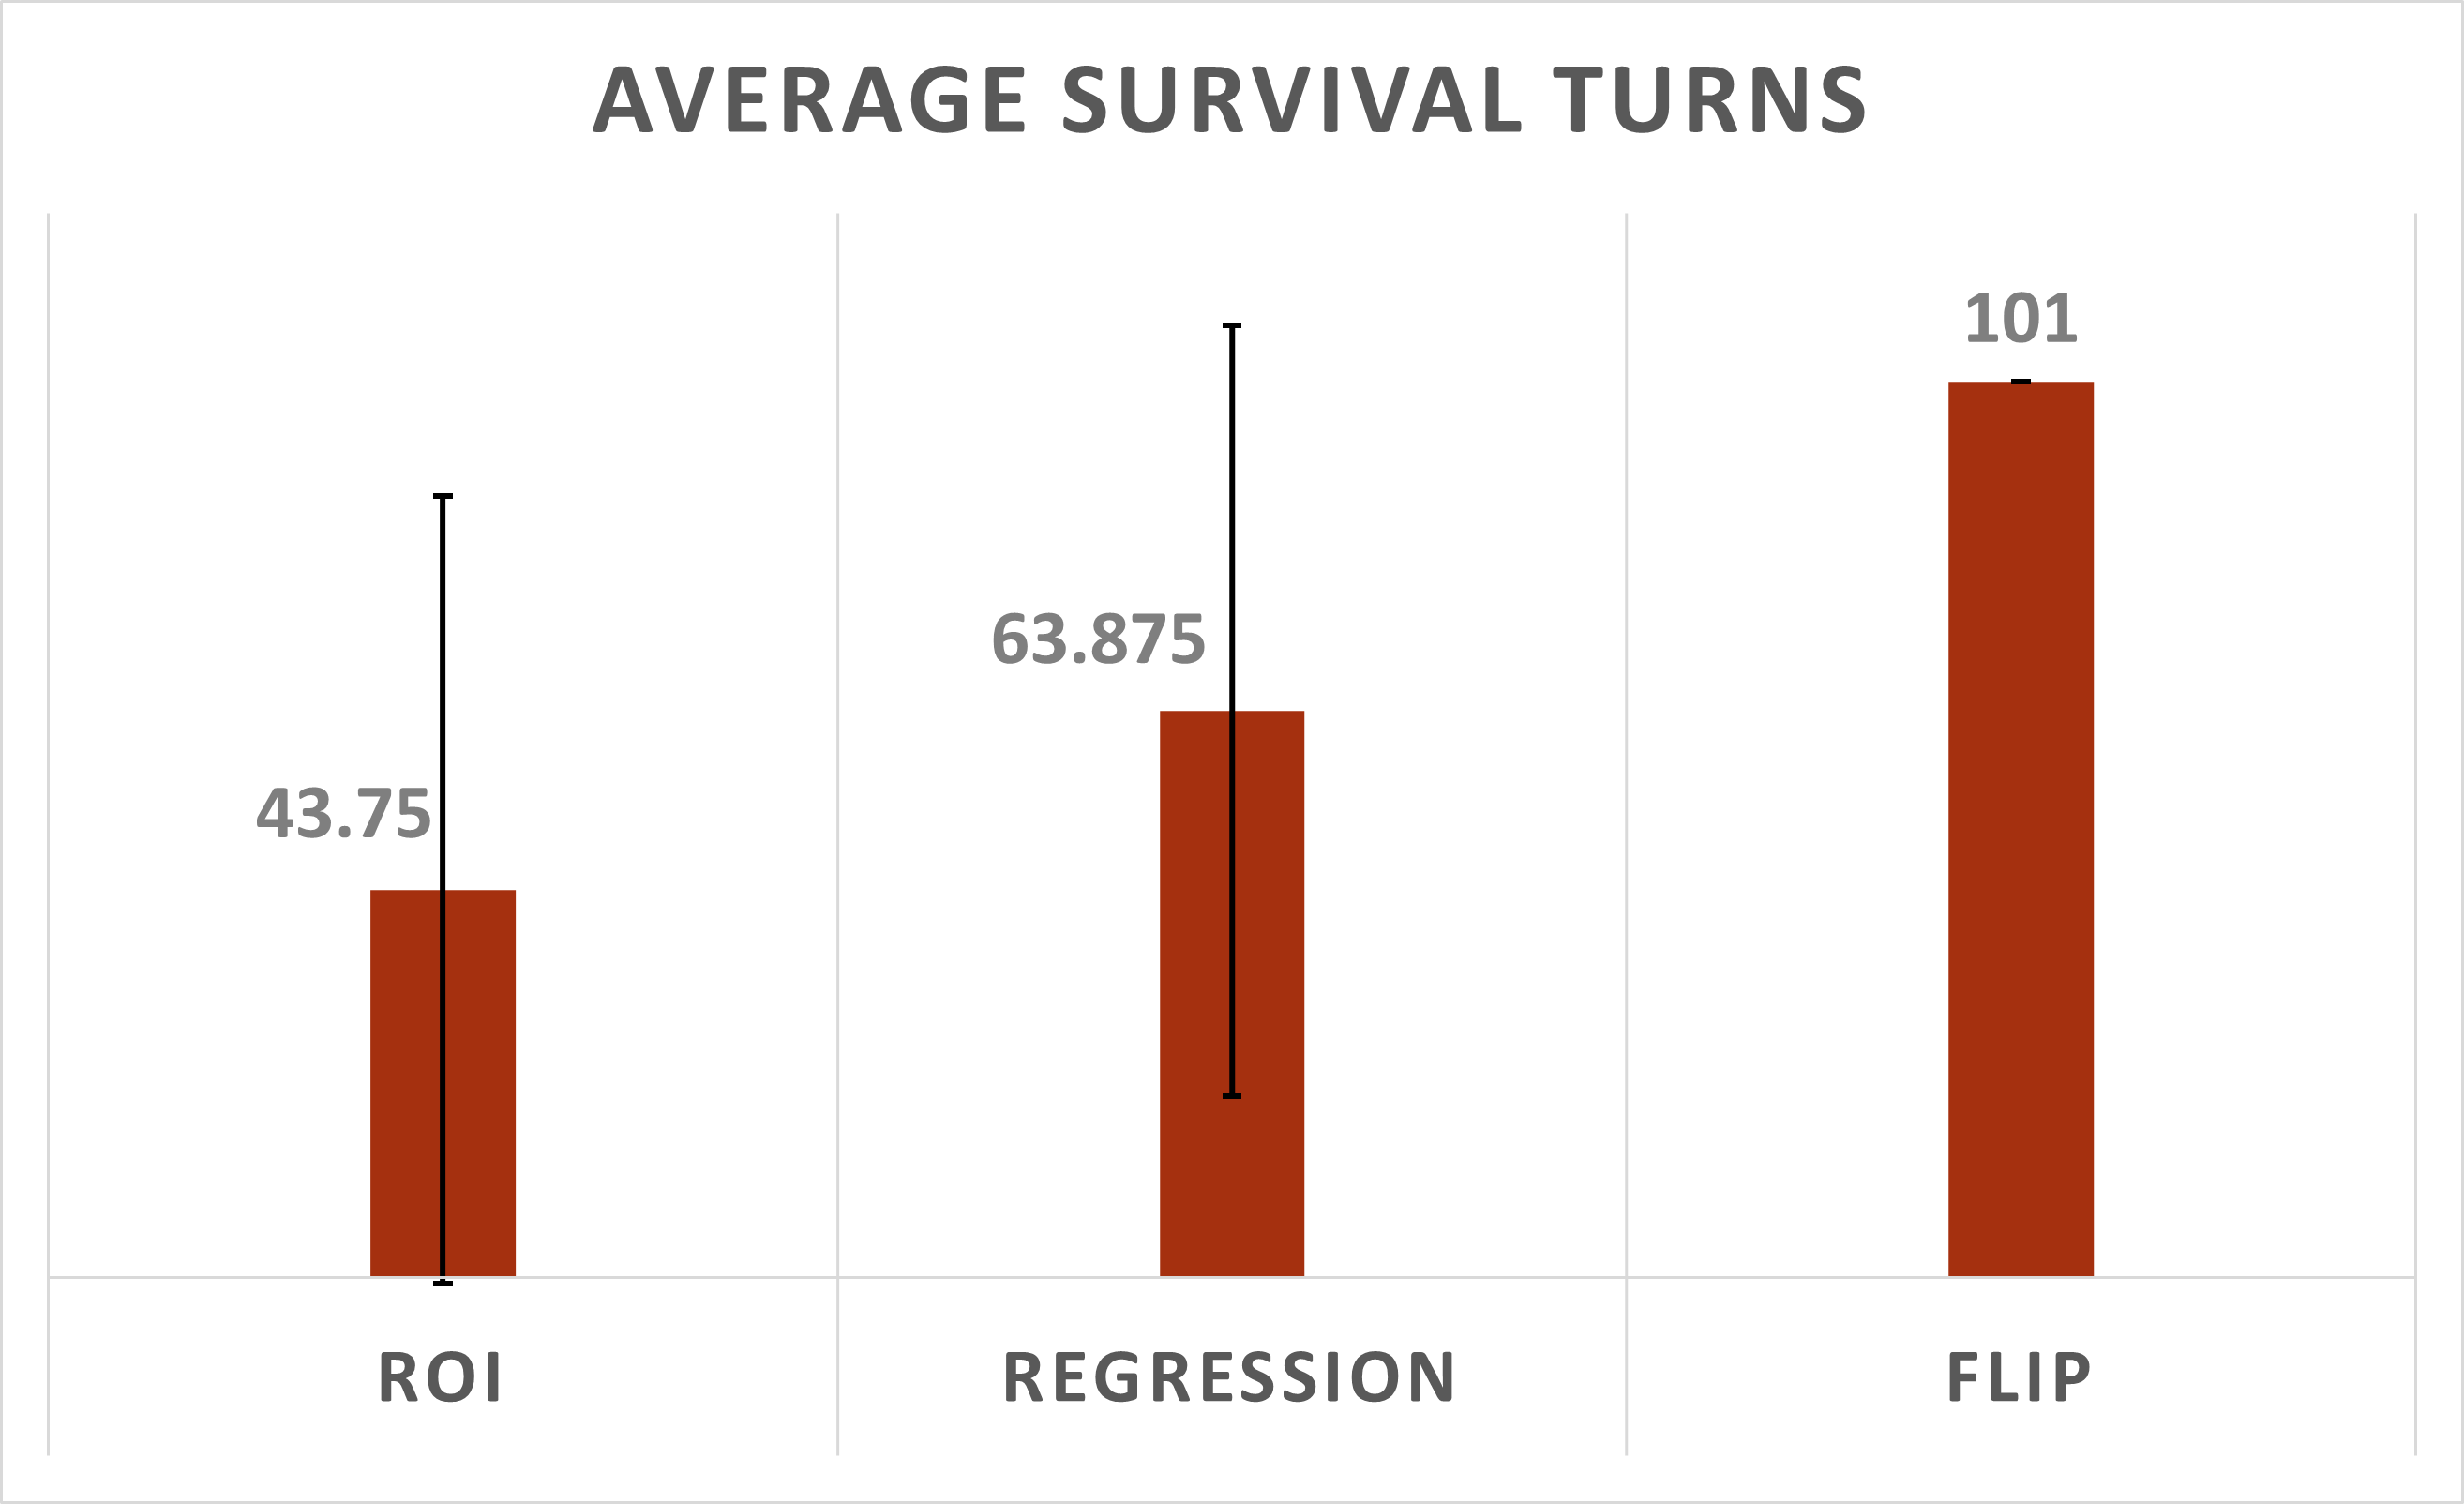
\includegraphics[width=0.6\textwidth]{09_team1_agentdesign/images/mean_survival_turns}
\caption{Mean survival turns for different strategies.}
\label{fig:team1:mean_survival}
\end{figure} 

\begin{figure}[H] 
\centering
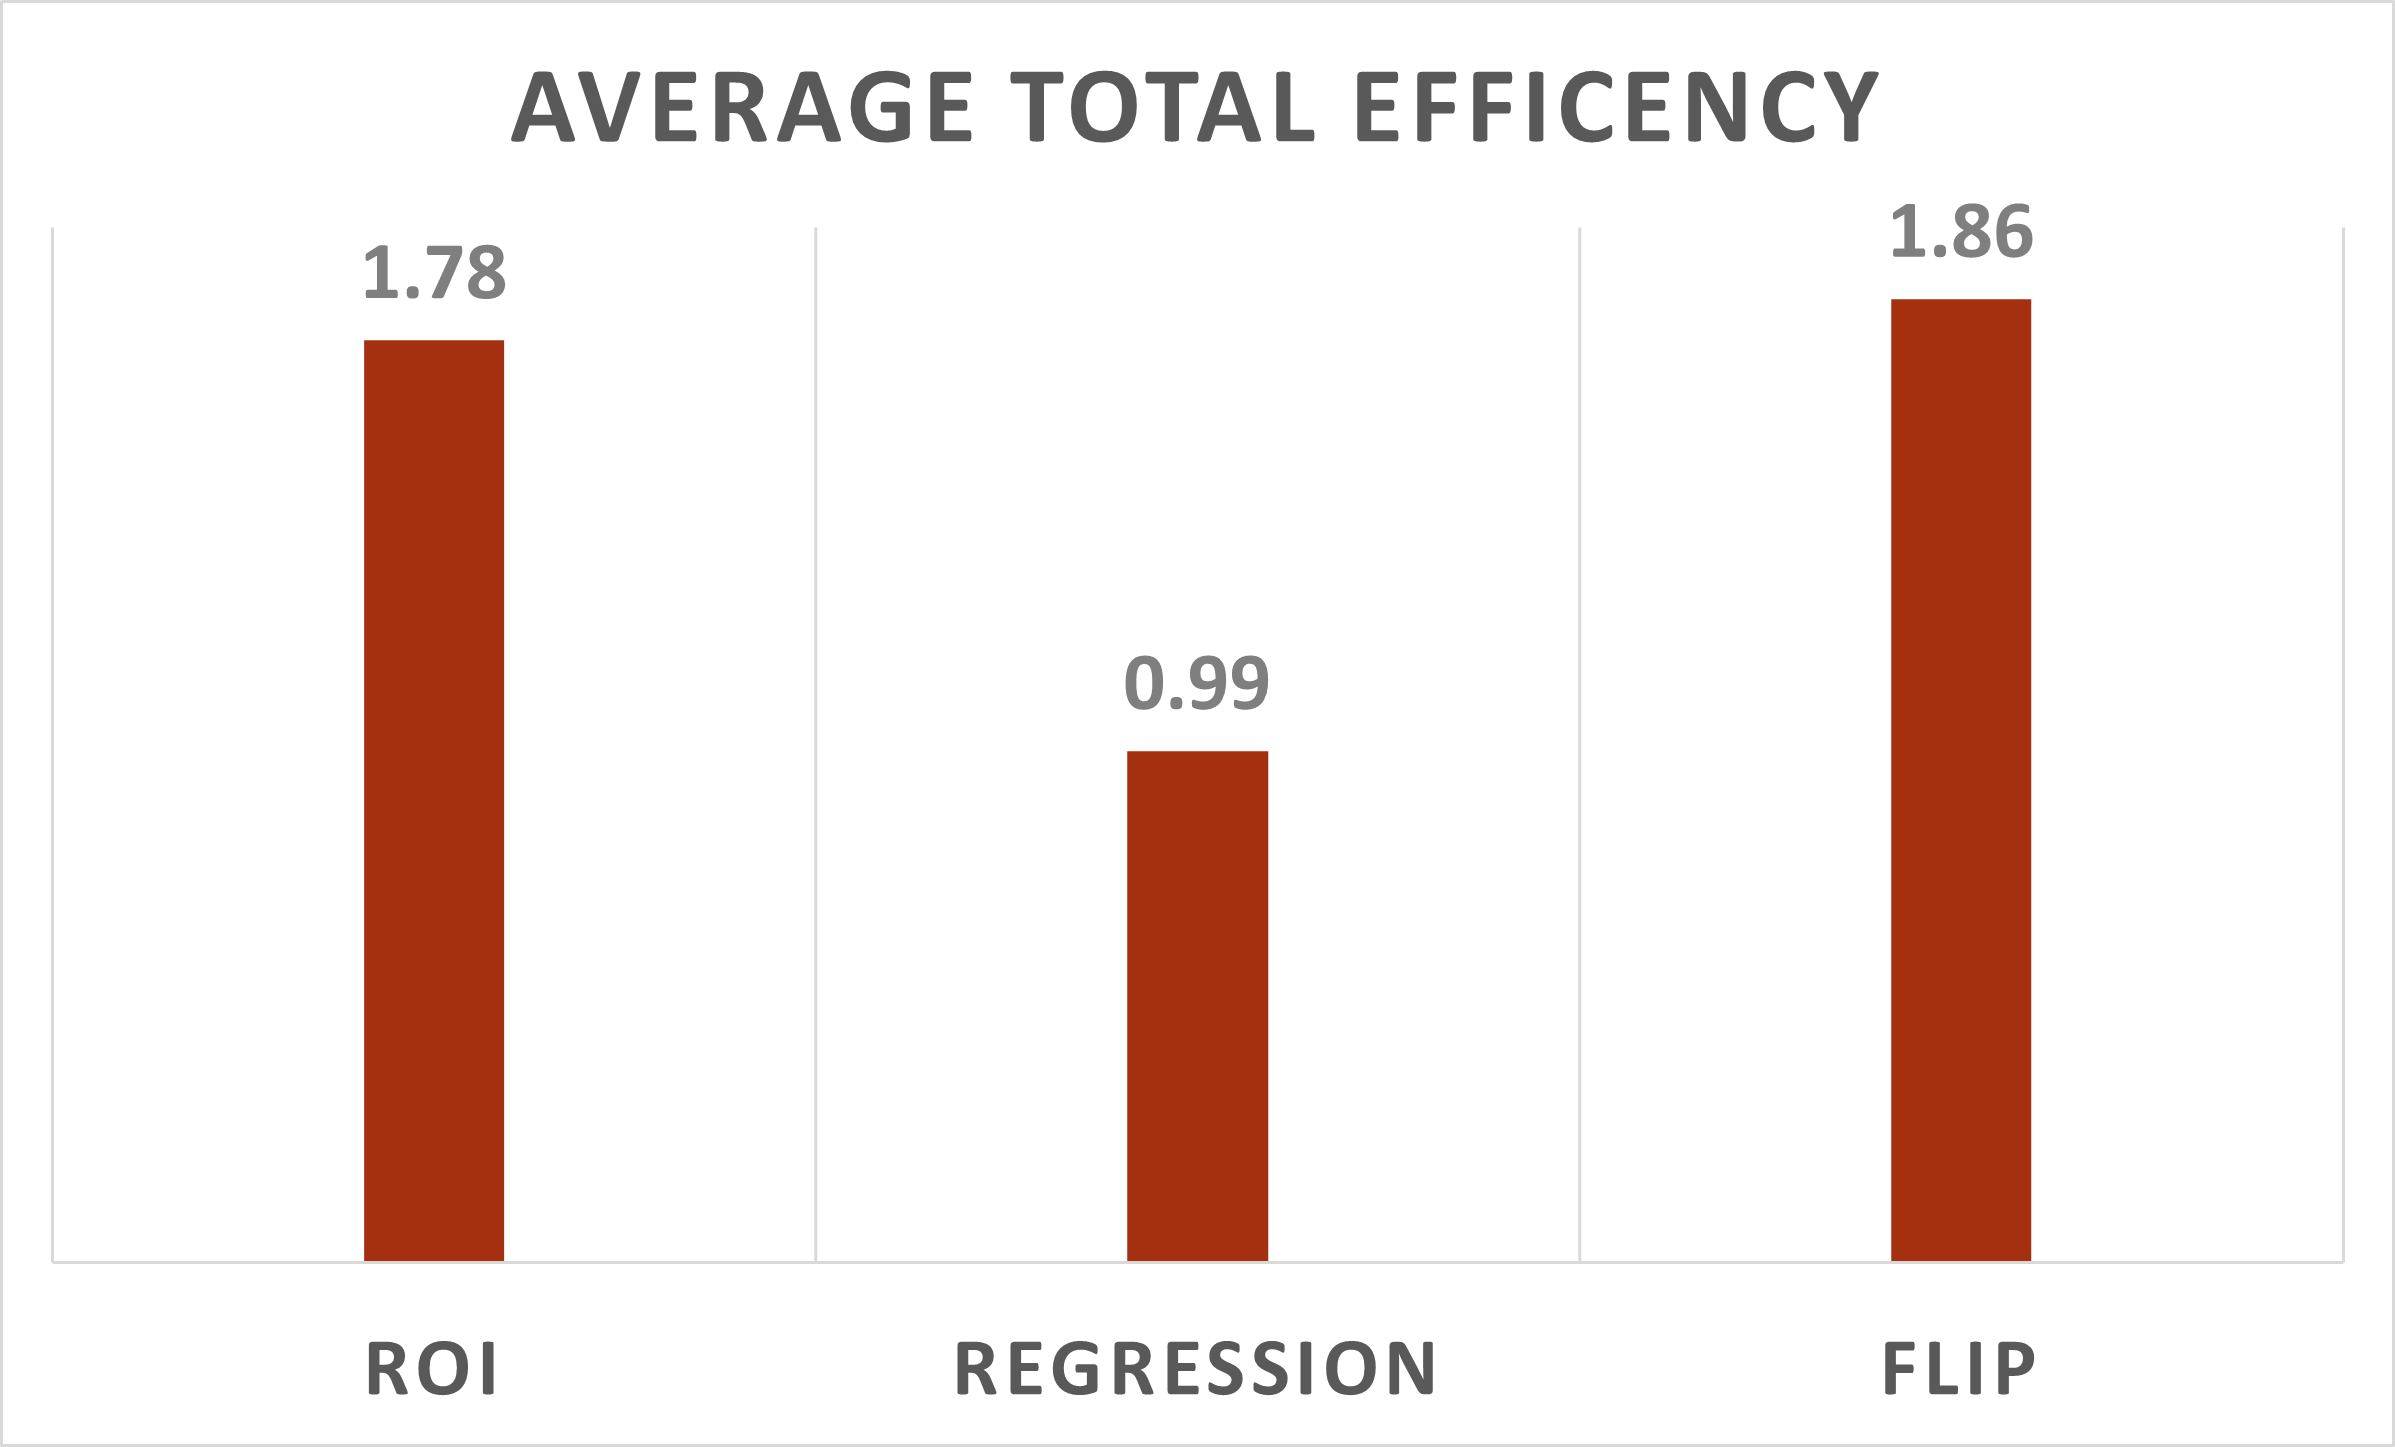
\includegraphics[width=0.6\textwidth]{09_team1_agentdesign/images/total_efficiency}
\caption{Average foraging efficiency}
\label{fig:team1:average_efficiency}
\end{figure} 

It is clear from \autoref{fig:team1:mean_survival} that the \emph{flip} foraging strategy dominates the other two in terms of overall effectiveness. However, it is interesting to note that, according to \autoref{fig:team1:average_efficiency}, the \emph{ROI} foraging method is almost as efficient as \emph{flip}, which raises the question of what causes the difference in their success. This difference could be attributed to one core issue with the \emph{ROI strategy}: ignoring the absolute value of rewards. The agent will happily settle for a profit of $11$ resources, if that was obtained with a contribution of $0.1$ resources (a profit of $110000\%$) over a profit $50$ resources for a contribution of $25$ (a measly $100\%$). This means that in the long run living costs overwhelm the \emph{ROI} agent. The \emph{flip} agent does not take expected profit into account and as such is unaffected by this.

\emph{Regression} appears to occupy a medium between \emph{flip} and \emph{ROI}, however it is much less consistent, as evidenced by the error bars in \autoref{fig:team1:mean_survival}, with \emph{regression} surviving for under 10 turns in some runs.

%%% Local Variables:
%%% mode: latex
%%% TeX-master: "../main"
%%% End:

    \chapter{Team 2 Agent Design}
\section{Overall Agent Strategy}

The overall strategy of our agent is based on a series of distinct, overlapping dilemmas. The agent operates on principles based on Evolutionary Economic Theory \footnote{https://www.cambridge.org/core/what-we-publish/elements/evolutionary-economics}. Game theory and the use of the Nash equilibrium also guided the development of the strategies implemented. The other top-level strategy which overlaps with several dilemmas is the social dilemma; this is when we quantify the relationship we have with other agents to produce trust and confidence levels. The interaction between the top-level strategies with all of the dilemmas is shown in Figure~\ref{fig: top level strategy}. The top-level strategy's implementation into each agent function and role is discussed in the following sections. 

\begin{figure}[!htb]
    \centering
    \begin{subfigure}{.49\textwidth}
        \centering
        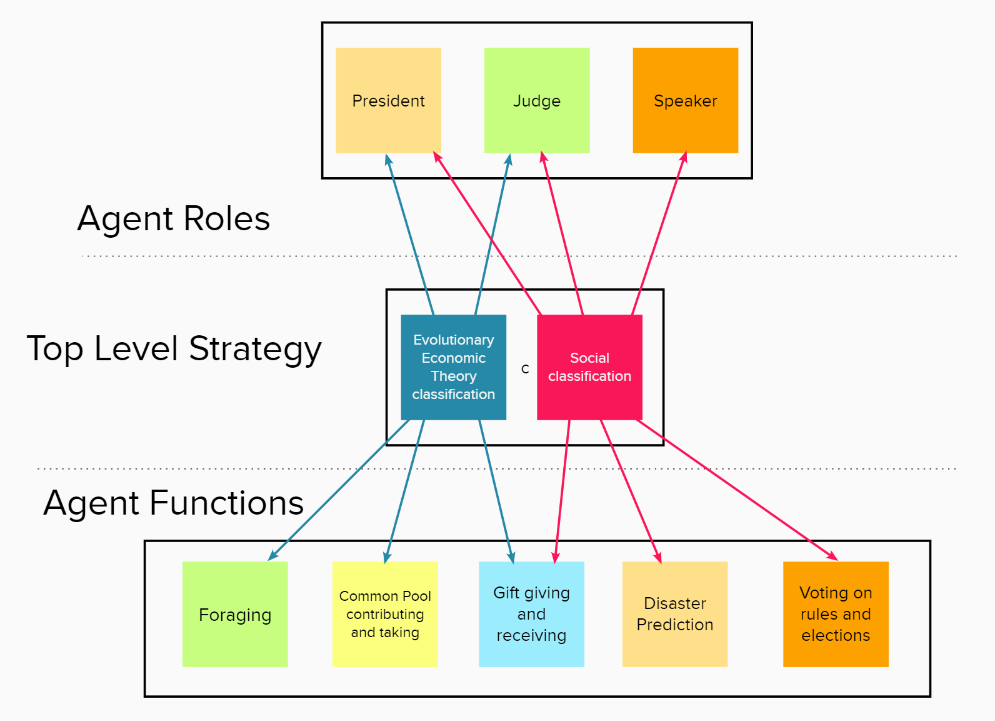
\includegraphics[width=0.99\textwidth]{images/strategies.png}
        \caption{Top level strategy}
        \label{fig: top level strategy}    
    \end{subfigure}
    \begin{subfigure}{.49\textwidth}
        \centering
        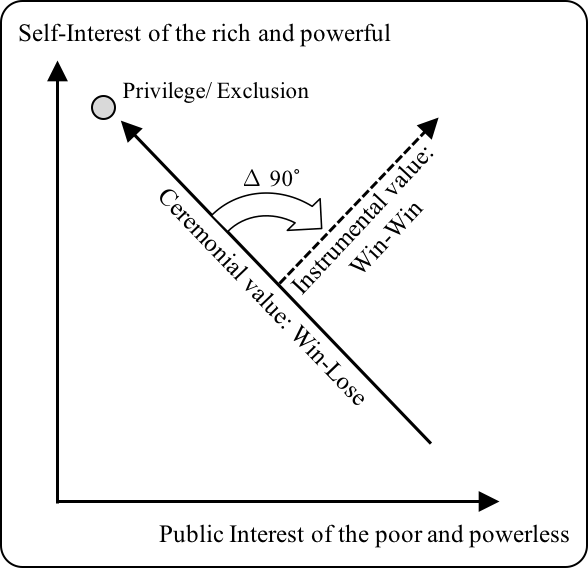
\includegraphics[width=0.9\textwidth]{images/dichotomy.png}
        \caption{Ceremonial-Instrumental dichotomy}
        \label{fig: dichotomy}
    \end{subfigure}
\end{figure}

\subsection{Evolutionary Economic Theory}
The term Evolutionary Economic Theory was first coined by economist Thorstein Veblen \footnote{https://www.cambridge.org/core/what-we-publish/elements/evolutionary-economics}. Evolutionary Economic Theory proposes that economic processes evolve, and it rejects the assumptions of classical rational choice theory. From Evolutionary Economic Theory, we categorised agent behaviour into distinct groups \footnote{https://www.cambridge.org/core/what-we-publish/elements/evolutionary-economics}. These groups are an altruist, fair sharer, and free rider. These are explained in Table~\ref{tab:Evolutionary Economic Theory Agent classifications}.

\begin{table}[!htb]
\caption{Evolutionary Economic Theory Agent classifications}
\label{tab:Evolutionary Economic Theory Agent classifications}
\begin{tabular}{|c|c|l|}
\hline
\textbf{Agent classification} & \textbf{Definition}                                                                                                                        & \multicolumn{1}{c|}{\textbf{Examples within the game}}                                                                                                        \\ \hline
Altruist                      & \begin{tabular}[c]{@{}c@{}}More concerned about the welfare \\ of the group than themselves\end{tabular}                                   & \begin{tabular}[c]{@{}l@{}}-Contributes a surplus to the common pool\\ -Generous with gifts\end{tabular}                                                     \\ \hline
Fair Sharer                   & \begin{tabular}[c]{@{}c@{}}Contributes enough to the group \\ to negate their negative impact on it\end{tabular}                           & \begin{tabular}[c]{@{}l@{}}-Contributes the minimum necessary amount of resources \\ -Gift allocation is measured and reasonable\end{tabular}                          \\ \hline
Free rider                    & \multicolumn{1}{l|}{\begin{tabular}[c]{@{}l@{}}More concerned with their individual \\ welfare than the welfare of the group\end{tabular}} & \begin{tabular}[c]{@{}l@{}}-Will not contribute enough to the common pool \\ -Gift requests above their requirement \\ -Will not give out gifts\end{tabular} \\ \hline
\end{tabular}
\end{table}

The advantage of using this theory over rational choice theory from classical economics is that it accounts for the irrational decisions agents or humans make when dealing with economic decisions, such as deciding how much to contribute to a common pool. Humans have evolved to develop heuristics \footnote{https://www.sciencedirect.com/topics/social-sciences/heuristics} which are "rules of thumb" in order to make economic decisions quickly and when all information is not present. These heuristics are typically based on emotion and will often result in irrational decisions; an example of this would be brand loyalty. This is very relevant within the context of the game because there is a cost to large computations (decision making). Also, there is an information failure \footnote{https://www.economicsonline.co.uk/Market_failures/Information_failure.html} as the agents often do not know the threshold of the common pool and other vital game metrics. This information failure forces agents to use heuristics similar to those used by real people. An excellent example of a heuristic within this agent strategy is the level of trustworthiness decided within the social dilemma. If every agent was rational and all information was present in the game, there is no need to trust or distrust agents as they would maximize both their welfare and that of others.

Another primary reason for selecting this theory as the basis of our design is to explore the ceremonial-instrumental dichotomy\footnote{https://www.jstor.org/stable/3486187?seq=3#metadata_info_tab_contents}. This dichotomy is best represented by the graph in figure \ref{fig: dichotomy} and shows the importance of the game's setup. Our agent is attempting to oppose this traditional response to instrumental and ceremonial societies. It would be interesting to change the game's ceremonial and instrumental values by changing the setup. While the current game infrastructure does not support this, it would be interesting to investigate the ceremonial-instrumental dichotomy by allowing islands to invest resources into developing their foraging technology to obtain higher returns. It would be interesting to investigate how this instrumental shift would change our agent's strategy and others' actions. This update in technology would replace the ceremonial institutional set up of the IIGO as it becomes redundant. Allowing islands to invest in technological advancement would add an extra dimension to the game as it evolves, and the importance of the IIGO and other instrumental components would shift.

\subsection{Evolutionary Economic Theory Implementation}
%explain how we use the information from the theory

Figure~\ref{fig:methods-of-play} shows the different states of our agent's different methods of play. At any point during the game, the state of our agent is determined only by the level of the Common Pool. Our agent's objective is to oppose the strategies employed by other agents to attain stability in the game. To determine the method of play of the other agents, we look at whether the Common Pool is, on average, increasing or decreasing. If the pool is being depleted, it can be assumed that the other agents act as free-riders on average. To counteract this, we act as an altruist (see section \ref{sec:Common Pool Dilemma Strategy} for more detail). The average pool level is used because individual agent strategies are irrelevant for the game's overall course. Within the game, we also do not always have access to individual agents' contributions, which would be needed to classify them individually. This makes the average level of the Common Pool the only viable parameter. 

Our simulations demonstrated that starting the game in a "free-rider" state resulted in optimal agent performance and did not negatively impact the course of the game overall.

The default state for the agent is to be a "fair sharer." The agent will move into altruist mode when the weighted average of the Common Pool has dropped drastically. The agent considers a weighted average to ensure that the agent does not panic after every disaster and over contribute. The most recent turns will also be weighed higher to determine the course of the game. When the Common Pool stops decreasing, the agent will move back to fair sharer mode. Similarly, if the pool's weighted average increases by a large factor, then our agent moves into a free-rider state.

\begin{figure}
\centering
\begin{subfigure}{.49\textwidth}
    \centering
    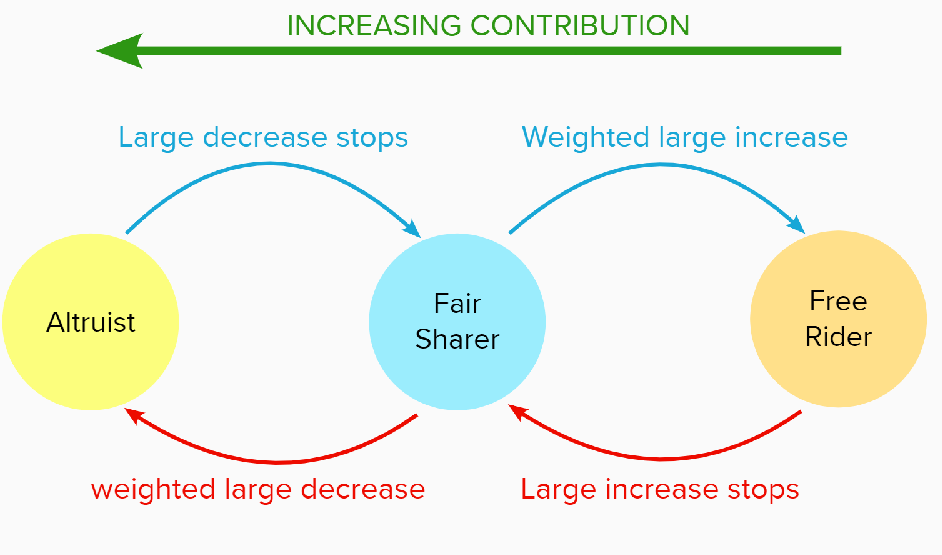
\includegraphics[width=0.9\textwidth]{images/MethodofPlay.png}
    \caption{Method of Play diagram}
    \label{fig:methods-of-play}
\end{subfigure}
\begin{subfigure}{.49\textwidth}
    \centering
    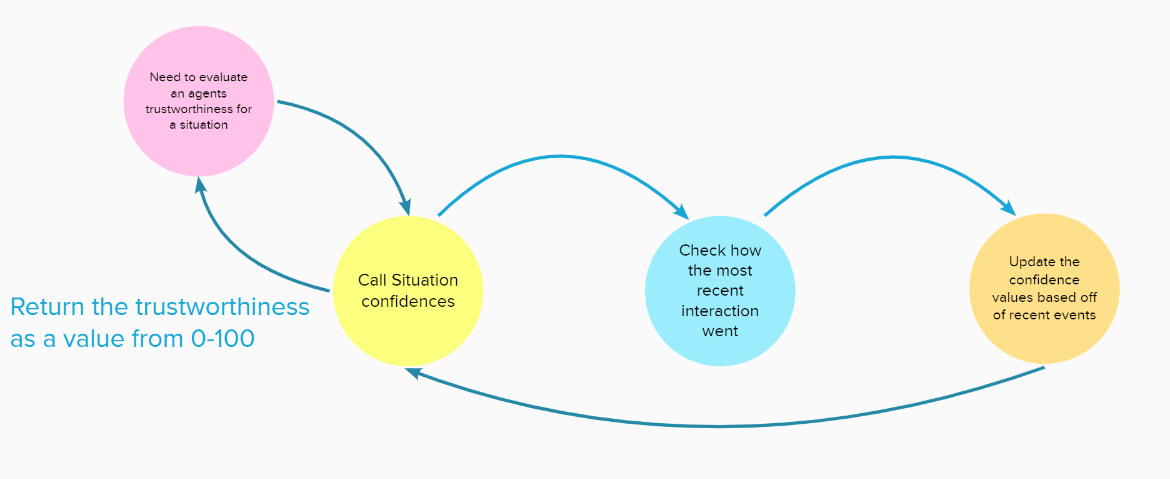
\includegraphics[width=0.9\textwidth]{images/Social.png}
    \caption{Social Classification Order}
    \label{fig:social-order}
\end{subfigure}
\end{figure}

\subsection{Social Classification}
The agent forms an opinion on others depending on different situations. Initial testing suggested that another island's gift-giving behaviour does not necessarily correlate with their quality of predictions. Consequently, the trust of other agents is computed and stored separately for each situation. The agent uses the weighted average of past interactions with other agents to determine whether or not to trust them in each situation for future interactions. Using a weighted average to compute trust resulted in notably better agent performance. This is because the agent's trust in other agents considers all interactions with other agents while weighting recent interactions more heavily.

An integer value represents the agent's trust metric for each agent in each situation between 0 and 100, where 100 denotes full confidence and 0 a complete lack thereof. This value is used to compute the expected outcomes of situations. These are then compared with real events to update the agent's confidence in the other agents regarding this situation. For example, when the agent receives predictions from other islands, it computes the weighted average to check whether it trusts the island. Once a disaster occurs, the magnitude or timing of the disaster is compared with the other island's prediction. This reality is used to assess their behaviour and update the trust metric for that island relating to that situation. The list of different "situations" includes how an agent behaves in a role such as the President, Judge, Speaker, gift-giving, and disaster prediction. The overall structure of how the agent forms opinions on other islands is shown in Figure~\ref{fig:social-order}.

\section{Gift Giving and Receiving}
The agent must decide whether or not to respond to other agents' gift requests and how much to request from others through gifting. The implementation does not consider whether or not an agent is critical when requesting gifts and instead considers its current method of play and the trustworthiness of the requesting agent. Figure~\ref{fig: gifts} shows a decision tree for how the agent will allocate or request gifts, in which the agent splits up the gift request among the other agents to increase the likelihood of an agent allocating the gift.


\begin{figure}[!htb]
    \begin{subfigure}{.49\textwidth}
        \centering
        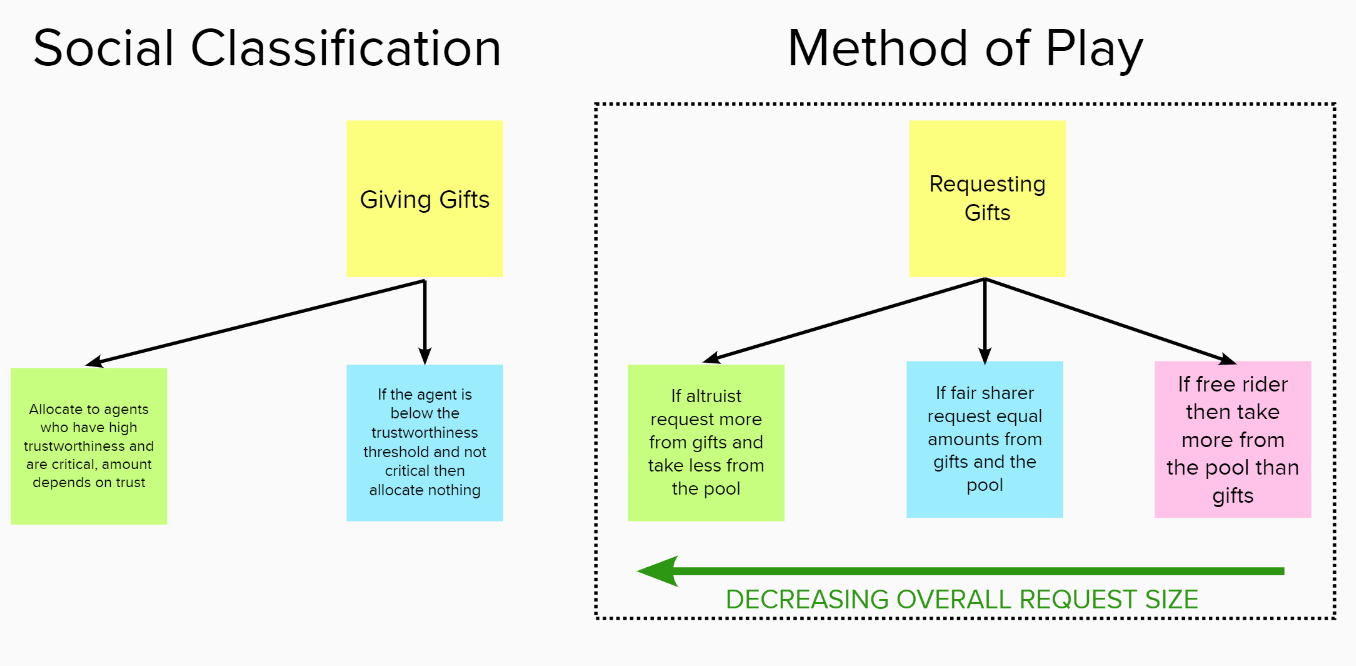
\includegraphics[width=0.99\textwidth]{images/gifts.png}
        \caption{Gift Giving and Receiving decision tree}
        \label{fig: gifts}
    \end{subfigure}
    \begin{subfigure}{.49\textwidth}
        \centering
        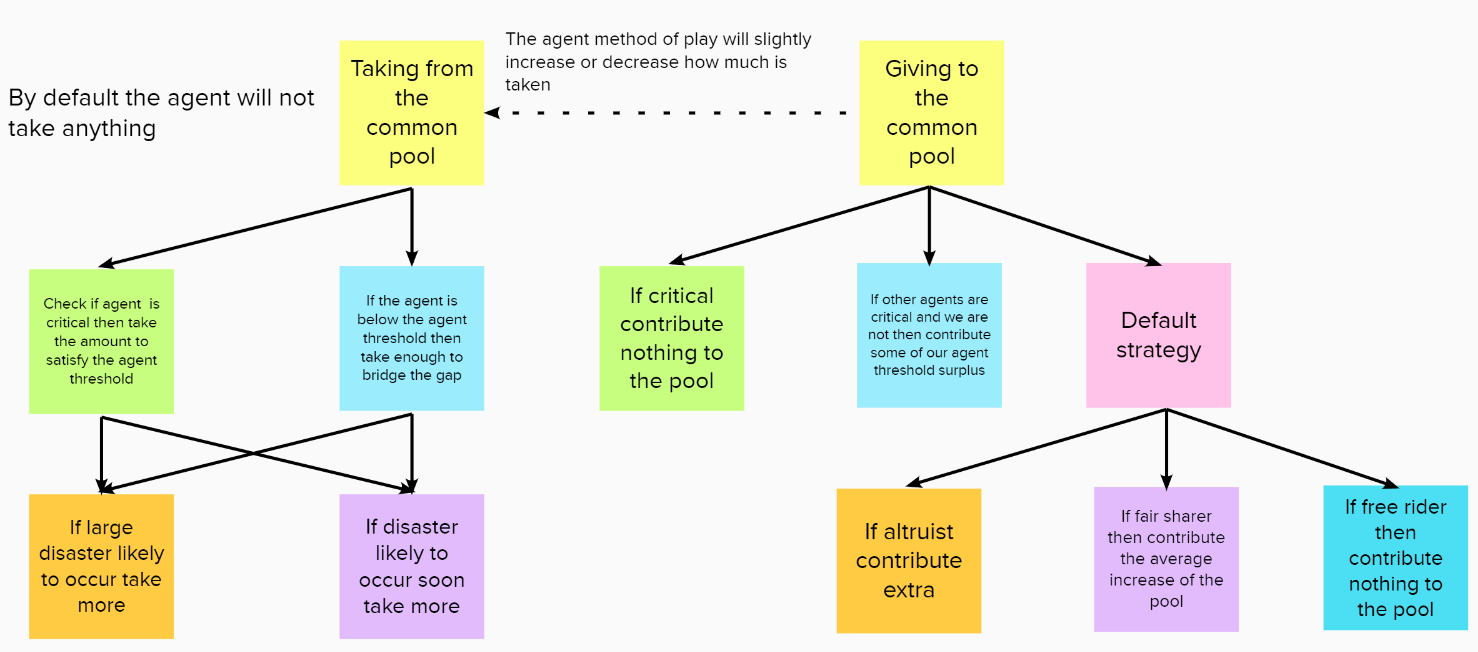
\includegraphics[width=0.99\textwidth]{images/common_pool_strategy.png}
        \caption{Common Pool Strategy}
        \label{fig: common_pool_strategy}        
    \end{subfigure}
\end{figure}

Depending on the method of play, the agent will request more or fewer gifts. This is inversely proportional to the number of resources taken from the Common Pool. The agent obtains a larger proportion of its needed resources from gifting than the Common Pool in the altruist state. This is done to mitigate common pool depletion in the interest of the common good. In a Fair-Sharer state, the agent aims to obtain its resource target equally from gifts and the Common Pool. A minor surplus is also included in the resource target to ensure that the goal is met, given that gifts from other agents cannot be guaranteed. In a Free-Rider state, the agent takes the majority of its resources directly from the Common Pool but still requests gifts to build up its resources by taking advantage of relationships with other agents as well as a Common Pool surplus.

The \textbf{Gifts} social classification situation refers to both when an island requests a gift from our agent and when our agent requests a gift from that island. The balance between agent gift requests and responses is used as a basis for opinion formation on another agent. Other agents that fulfill the agent's requests are rewarded with higher trust. The agent's own gift requests tend to be small but are also proportional to its trust in each other agent. Every gift interaction is used to update the agent's trust in another island's gifting behaviour.

\section{Common Pool Dilemma Strategy} \label{sec:Common Pool Dilemma Strategy}
The Common Pool dilemma strategy can be split into two considerations. One consideration is the current method of play (altruist, fair sharer, and free-rider), and the other is the current game state. A decision tree showing the common pool strategy is shown in Figure~\ref{fig: common_pool_strategy}. These considerations decide whether and how much we contribute or take from the Common Pool.

\subsection{Method of play consideration} \label{ssec:Method of play consideration}
The primary consideration for giving to the Common Pool dilemma is the agent's current method of play. The agent's state is determined by the Common Pool level, as seen in Figure~\ref{fig:methods-of-play}. The agent's default state as a "fair sharer" contributes the average amount of other agents to the Common Pool. This is calculated by evaluating changes in the Common Pool level from the previous turn and averaging this quantity by dividing by the number of alive agents. If the Common Pool level decreases, the most recent Common pool increase is used to determine the amount given.

By using the average Common Pool contribution, the agent benefits from the forecasting of other agents. This benefit would arise should another agent have an advanced forecasting prediction that determines the Common Pool threshold and what is required to mitigate the effects of a disaster. In this case, the agent would then contribute a similar quantity of resources. This "herd-mentality" approach relies on the assumption that other agents make rational decisions. So if it is evident that other agents are acting irrationally, the agent deviates from this approach to an alternative state (to become either a free-rider or an altruist).

The agent is in an altruist state when the Common Pool is struggling, which often means that other agents act as free-riders. This is where the meta-strategy of Evolutionary Economic Theory comes into play. It is in the agent's interest to contribute much more to the Common Pool to alter the game's course in a positive direction and prevent the pool from being below the threshold when a disaster occurs. Therefore, the agent contributes more resources to enact this balance on the system. 
The altruist resource contribution is a larger factor of the weighted average contribution and can be tuned using the \emph{altruist factor} variable in the agent's configuration.

In a free-rider state, the Common Pool has a surplus, and the agent assumes other agents are on average operating as altruists. In this situation, the agent contributes less to the Common Pool and preserves resources to mitigate short and long-term risk. Contributing too much to the Common Pool no longer benefits the greater good, as these resources can still be used to forage and generate more resources. Therefore, the agent accumulates resources when others are too generous, allowing greater foraging investments and making it easier to help other agents if they struggle in the future.

The method of play also impacts how the agent decides to take from the Common Pool. After game state considerations are made, the agent adjusts how much it takes from the Common Pool according to its Agent State. Table~\ref{tab:Method of play common pool taking} outlines a summary of how the agent adjusts how much it takes and gives a justification for each action. The amount to take from the pool depends on how willing other agents are to contribute to the agent within the game's gift-giving section.  This means the agent must decide what proportion of the resource request must be taken from the Common Pool and from gifting, and this decision also factors in both common pool allocation as well as gift response predictions. When the agent is in a free-rider state, the common pool has a surplus, and so it makes more sense to take directly from the pool rather than requesting gifts. 

\begin{table}[!htb]
\centering
\caption{Method of play common pool taking}
\label{tab:Method of play common pool taking}
\begin{tabular}{|c|c|}
\hline
\textbf{Agent classification} & \textbf{How this impacts taking from the common pool}                              \\ \hline
Altruist                      & Pool is being depleted, best to not take from the pool                             \\ \hline
Fair Sharer                   & Gift requests and taking from the pool are equal                                   \\ \hline
Free rider                    & \multicolumn{1}{l|}{Pool has surplus, take from the pool rather than gift request} \\ \hline
\end{tabular}
\end{table}

\subsection{Game state consideration} \label{ssec:Game state consideration}
The primary consideration in taking from the Common Pool is the current game state. The key parameters (shown in Figure~\ref{fig: common_pool_strategy}) considered are whether the agent is critical and whether the agent has excess resources. This excess is calculated as the difference between the agent's current resources and the minimum resource threshold and the cost of living. Beyond this minimum resource level, the agent can survive one another turn. If the agent has fewer resources than these aggregated costs, the excess is zero. If there are excess resources, the agent will give some resources to the Common Pool. In this case, a strategic contribution is calculated. If the Common Pool threshold is known, the agent considers how many resources are required to attain this threshold. This is then spread over the expected number of turns until the next disaster is predicted to occur and the number of alive clients. If this is unknown, a default value is used to form an initial guess in the agent configuration. On top of this quantity, a strategic contribution is also calculated (see \ref{ssec:Method of play consideration}). The current method of play determines whether the disaster-determined contribution or the strategy-determined contribution is contributed to the pool. This amount is then contributed together with the current tax, unless there are no excess resources as this implies the agent is in a critical state and so all resources are preserved.

\section{Foraging Dilemma}
The foraging dilemma is split into two parts. One determines whether the agent should hunt or fish, and the other determines how many resources to spend on foraging. The foraging dilemma only depends on the current method of play. The method of play will impact the amount the agent uses to forages. If the Common Pool is doing well and the agent acts as a free rider, it will be more prone to take risk and contribute more to the foraging and vice versa. The decision to hunt or fish depends on the likely number of hunters in the next foraging event. The decision tree, Figure~\ref{fig: Hunt or fish decision tree }, shows how the agent decides whether to hunt or fish in a given turn. To determine the number of hunters in the next forage turn, the agent tracks how often each agent is a hunter and then sums up the probability of each agent hunting to find an overall number of likely hunters. The agent outputs a random number from 0 to 1, and if the number lies above the threshold, the agent will hunt. This threshold is determined by the number of likely hunters in the foraging. It implies there is an element of randomness to the agent's decision making, which will account for the unpredictability of dealing with other agents with their strategies.

\begin{figure}[!htb]
    \centering
    \begin{subfigure}{.49\textwidth}
        \centering
        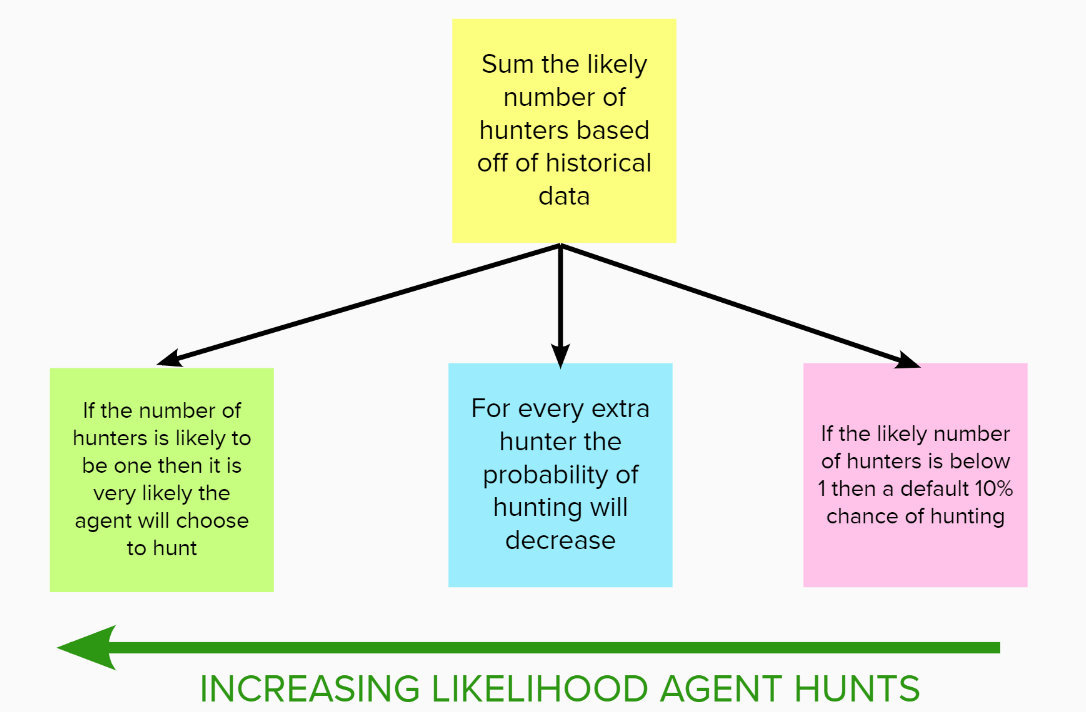
\includegraphics[width=0.9\textwidth]{images/forage_decision.png}
        \caption{Hunt or fish decision tree }
        \label{fig: Hunt or fish decision tree }
    \end{subfigure}
    \begin{subfigure}{.49\textwidth}
        \centering
        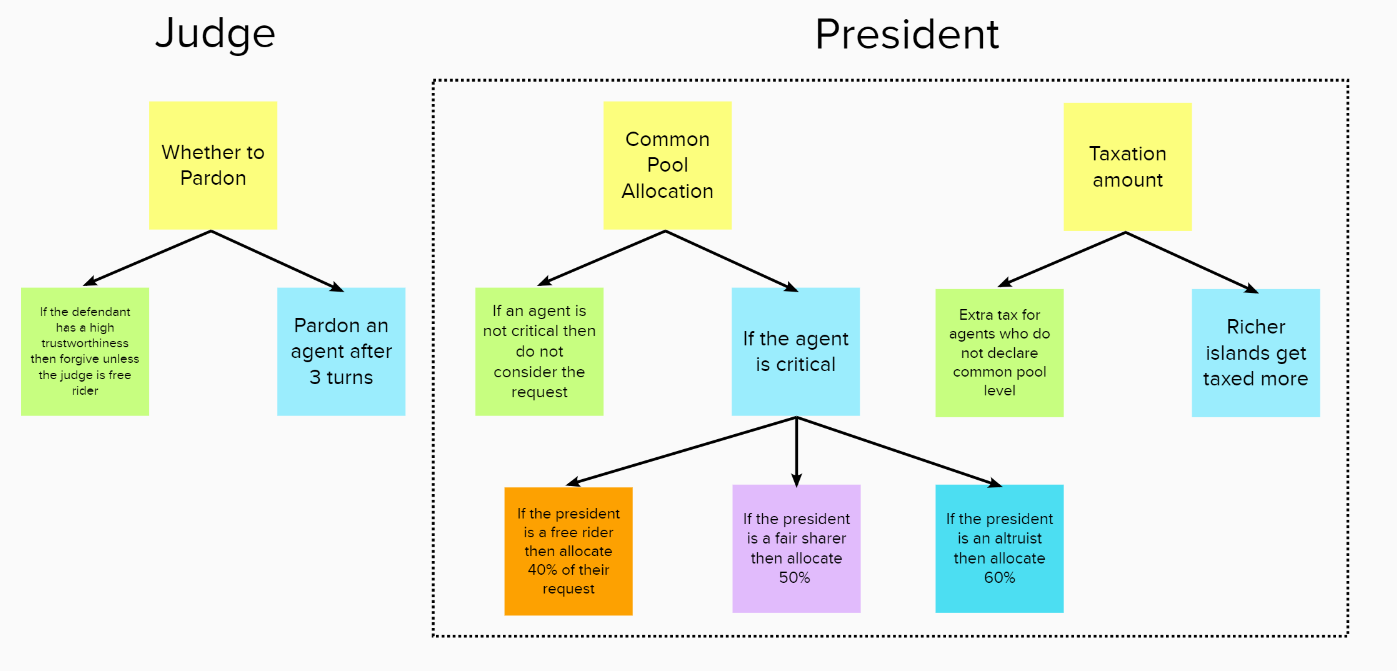
\includegraphics[width=1.0\textwidth]{images/Roles Decision Tree.png}
        \caption{Roles Decision Tree}
        \label{fig: Roles Decision Tree}        
    \end{subfigure}
    \caption{Hunting or Fishing and Roles Decision Tree}
\end{figure}

The ideal distribution for foraging is to have two agents hunting and the remainder fishing. Hence, when the agent predicts one other agent will hunt, the agent is highly likely to choose to hunt too. The default threshold for hunting is 0.1, so the agent will hunt 10\% of the time when not considering the likely number of hunters. By assuming that any agent will hunt or fish with equal probability, the likelihood that there is one hunter is approximately 0.16. This implies hunting is an optimal strategy approximately 16\% of the time, so a threshold similar to this value is chosen. If the predicted number of hunters is above one, the following equation is used to determine threshold placement: $\text{Probability of agent hunting} = 0.95 - \text{Predicted number of hunters} \times 0.15$

The probability of choosing to hunt when the agent is confident only one other agent will also select hunt is 0.95. For each additionally predicted hunter, the probability will fall by 0.15. This 0.95 threshold is included in the agent configuration so it can be edited without changing the code. Hence, the foraging decision can be tuned. The agent checks if there are any excess resources after considering the minimum resource threshold not to be critical and the cost of living. If there are no excess resources, no resources are spent on foraging. If there is an excess of resources, a percentage of this excess is used on foraging. This percentage is controlled in the agent configuration. This approach ensures the agent has enough resources to survive another round, even in the worst case scenario when foraging returns are minimal.

\section{Role Strategies}

Figure~\ref{fig: Roles Decision Tree} shows a decision tree of how the agent acts under the two roles implemented. Due to time constraints, the base client implementation was used for the Speaker. The President is responsible for allocating resources from the Common Pool based on agent requests. The agent uses game state variables such as their critical status to determine if another agent is worthy of their resource request and the agent's allocation method based on the method of play is outlined in Table~\ref{tab:President allocation method of play}. When the agent is in a free-rider state, it is more selfish, while when it is an altruist, more of the others agents requests are approved. If an agent is not critical, it is highly unlikely that the agent will allocate them their requested resources as the purpose of the Common Pool should be to primarily mitigate the effects of disasters. Resources are allocated on a need-first basis, taxed proportionally to an agents resource level, and the strategy to determine taxation includes an additional penalty tax for agents who do not declare their resource levels. When evaluating another President's performance, the agent considers the percentage change in tax, the percentage of how much the agent is allocated with respect to how much it requests, and how much the agent takes with respect to how much the President allocates it.

\begin{table}[!htb]
\centering
\caption{President allocation method of play}
\label{tab:President allocation method of play}
\begin{tabular}{|c|c|}
\hline
\textbf{Agent classification} & \textbf{\% of request given} \\ \hline
Altruist                      & 60                           \\ \hline
Fair Sharer                   & 50                           \\ \hline
Free rider                    & 40                           \\ \hline
\end{tabular}
\end{table}

The agent implementation of the Judge evaluates whether an agent has broken any rules, as it should. However, to model real world corruption, the agent does not sanction agents that break rules if it considers them to be highly trustworthy (i.e., with a trust score above 80\%). The agents behaviour as a Judge is also determined by its state; when the agent is a free-rider, it sanctions fewer islands. The \textbf{Judge}'s situation, similar to the President, is used by the agent to determine what island to vote for as Judge. This is done by checking the past sanctions the agent received and their duration, to maxmimise personal benefit. The \textbf{RoleOpinion} social classification situation is used when the agent is the Judge and must decide whether or not to pardon other islands' sanctions, whom to choose as the next President whether or not an island has adhered by the rules. The Judge receives information for each island, such as the difference between how much an island contributed to the common pool and how much said they would. The agent uses these differences as a Judge to determine whether or not an island is trustworthy. During a role election, the agent checks its trust in the candidates for the appropriate situation, i.e., the situation when an agent is "President" for a future Presidential election. The agent will return a list of candidates in decreasing order of preference determined by the social classification. To do this, the agent sorts the candidates in terms of how much it trusts them.

\section{Disaster Prediction}
It is important for the agent to be capable of predicting both the severity and timing of disasters, in order to effectively make decisions for contributing to both the common pool and gifting resources to other agents.

Since the simulation is constructed through a series of successive turns, the occurrence of disasters throughout the game can be seen as a Binomial distribution: $D \sim \text{Bin}(n,p)$. In this equation, $D$ describes the number of disasters that occur, $n$ is the number of turns played and $p$ is the probability of a disaster occurring on a given turn.

The aim of our agent is to estimate the number of turns between disasters. We will denote this random variable as $T_D$, with our agent's aim being to find $E[T_D]$. To do this, our agent must estimate $p$. Therefore we have programmed our agent to find the Maximum Likelihood Estimator of $p$ for a Binomial RV\footnote{https://stats.stackexchange.com/questions/191444/variance-in-estimating-p-for-a-binomial-distribution}: $\hat{p} = \frac{D}{n} = \bar{X}$, where $\bar{X}$ is the sample mean of the RV $X$. The expectation of $T_D$ can be estimated using\footnote{https://math.stackexchange.com/questions/1299465/proof-variance-of-geometric-distribution}: $\hat{\mu}_{T_D}= \frac{1}{\hat{p}} = \frac{1}{\bar{X}}$. Thus, this is the optimal estimator for our agent to predict the number of turns between disasters. Furthermore, the confidence that our agent has in this prediction should be inversely proportional to the variance of $T_D$, i.e. how much does $T_D$ vary from the expected value we have found above? The expression for this variance is given below$^2$: $Var(T_D)= \frac{1-p}{p^2}$. 

However, given that our agent does not know the actual value of $p$ used in the simulation, our agent instead estimates the variance using: $\hat{\sigma}_{T_D}^2= \frac{1-\hat{p}}{\hat{p}^2}$. Now that an expression for the estimate of this variance has been obtained, two questions remain: ``what about the variance in $\hat{p}$" and ``how is this variance translated into a confidence value?" The variance of $\hat{p}$ is given by the following expression: $Var(\hat{p})= Var(\bar{X}) = \frac{Var(X)}{n}$. As previously, we do not know the exact value of $p$, making a calculation of $Var(X)$ impossible. However, we can make use of the fact that $Var(\hat{p}) \propto \frac{1}{n}$, by making our agents confidence in the prediction proportional to $n$ also. Secondly, the fact that variance can take values $\in [0,\infty]$ but confidence must take a value $\in [0, 100]$ makes mapping the values of variance that our agent calculates, to a confidence level, challenging. The solution our team opted for was to cap the max value of variance to some value $v_{cap_{T_D}}$, before translating this variance into a corresponding confidence value. This process is given by the equation below: $\text{confidence}_{T_D} = 100 - \frac{100 \cdot \text{min}(\frac{\hat{\sigma}_{T_D}^2}{kn}, v_{cap_{T_D}})}{v_{cap_{T_D}}}$ 
where $k$ is the tuning parameter for altering the dependence of the confidence on $n$. 

\subsection{Magnitude Prediction}
Our agent's strategy for predicting the magnitude of the next disaster shares many similarities with the strategy discussed in the last section. However, the magnitude of the next disaster is now distributed with an Exponential distribution: $M \sim Exp(\lambda)$. Once again, start by finding the MLE for the parameter $\lambda$ \footnote{https://en.wikipedia.org/wiki/Exponential\_distribution}: $\hat{\lambda} = \frac{1}{\bar{M}}$. Now we seek to estimate the expectation of $M$: $\hat{\mu}_M = \frac{1}{\hat{\lambda}} = \bar{M}$. Similarly, the variance of this RV is also useful to estimate $\hat{\sigma}_{M}^2= \frac{1}{\hat{\lambda}^2}$. As previously, there is also a variance in our estimation of $\hat{\lambda}$ that must be taken into account by making our confidence in this prediction proportional to $n$. Thus, the following expression should be used for calculating the confidence in the magnitude prediction: $\text{confidence}_M = 100 - \frac{100 \cdot \text{min}(\frac{\hat{\sigma}_{M}^2}{gn}, v_{cap_M})}{v_{cap_M}}$, where $g$ is the tuning parameter for altering the dependence of the confidence on $n$. 

\subsection{Overall Prediction}
The overall prediction that must be shared with teams during the IIFO session requires the following information: location, time until next disaster, magnitude and confidence. For our prediction of location, the middle of the archipelago is always given since the probability of a disaster occurring at a given location is uniform across the archipelago, meaning that there is no optimal prediction formula. Using the findings presented in the above sections, the formulas our agent will use to form a prediction about the next disaster are as follows:

\begin{align*}
    &x_{coord} = x_{min} + \frac{(x_{max}-x_{min})}{2}, y_{coord} = y_{min} + \frac{(y_{max}-y_{min})}{2}, \text{conf} =\frac{\text{conf}_{T_D} + \text{conf}_M}{2} \\
    &\hat{\mu}_{T_D}=\frac{1}{\bar{X}}, \hat{\mu}_M = \bar{M} \\
\end{align*}

\subsection{Combined Prediction}
Generating our own prediction is only the first part of the prediction making process. The second stage is to make use of other island's predictions during the IIFO session and using the social classification to decide prediction accuracy. When considering how much emphasis to put on a given island's prediction, we make use of two factors: 1.) Our island's confidence in each other island's prediction making. 2.) Each island's confidence in their own prediction, $P_i \in [0,100]$. These two considerations are then combined to create an overall confidence factor.

\section{Simulations}
Every function and agent consideration has tuneable parameter which can be edited without changing the whole agent. Figure~\ref{fig: Forage Untuned} shows how our agent reacts when it plays against itself and the foraging parameters are untuned. As you can see the game is unstable and the agents have a low survival rate. This is caused by an over contribution to the foraging dilemma, there is a point of marginal return with the foraging dilemma and spending too many resources can be wasteful. 

\begin{figure}[!htb]
    \centering
    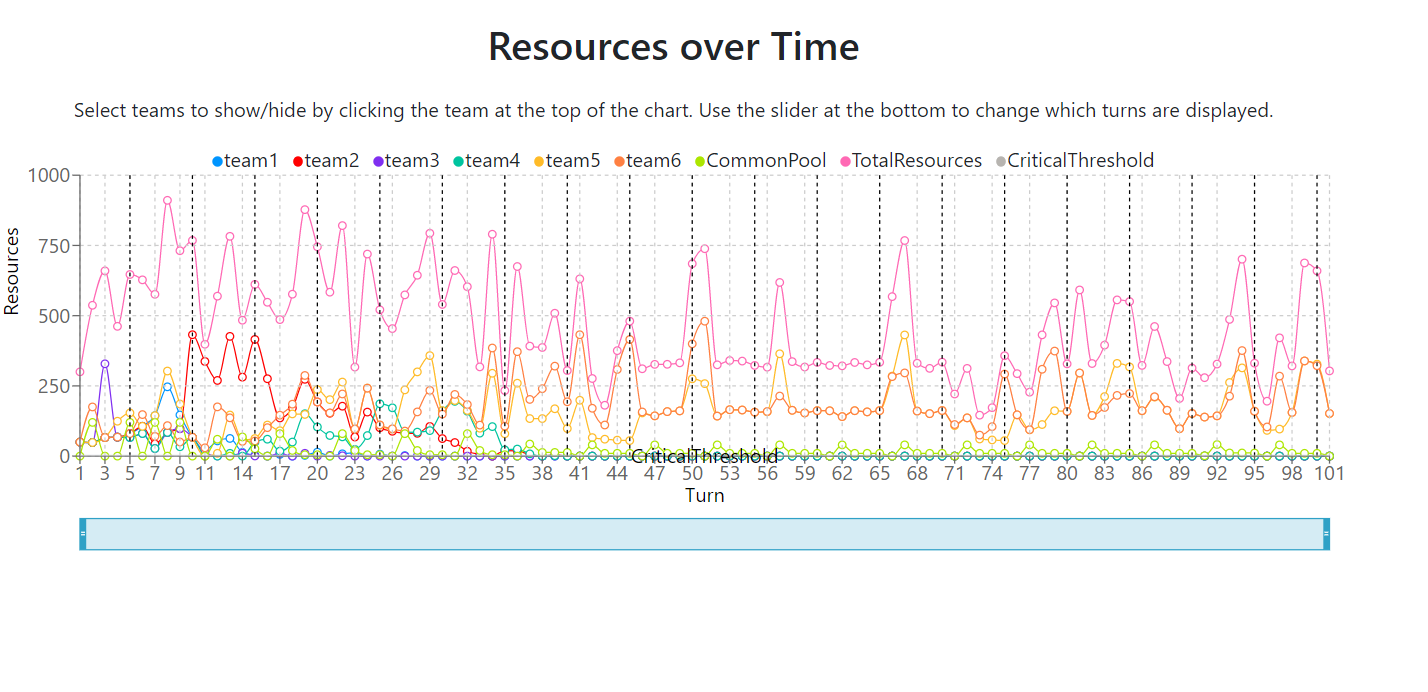
\includegraphics[width=0.6\textwidth]{images/Forage Untuned.png}
    \caption{Untuned Forage Simulation}
    \label{fig: Forage Untuned}
\end{figure}

Figure~\ref{fig: Forage tuned} shows how our agents plays against itself when the foraging parameters are optimised. The amount of excess resources spent on foraging is more reasonable in this simulation, this results in a much higher survival rate and a more stable common pool.

\begin{figure}[!htb]
    \centering
    \includegraphics[width=0.6\textwidth]{images/Forage tuned.png}
    \caption{Tuned Forage Simulation}
    \label{fig: Forage tuned}
\end{figure}

Figure~\ref{fig: altruist sim}  shows what happens when the agent plays itself and they are all altruists by default and do not move out of altruist. It can be seen that the agents over contribute to the Common Pool and are left with nothing to forage, this ends the game rather quickly. The simulation result was very similar for when all of the agents were free riders, the game would end in a couple of rounds after a lack of contribution to the common pool which caused impactful disasters.  This proves that being a free rider or altruist is not a rational decision and must be avoided. 
%the other graph is not really as expected so lets just keep it like this

\begin{figure}[!htb]
    \centering
    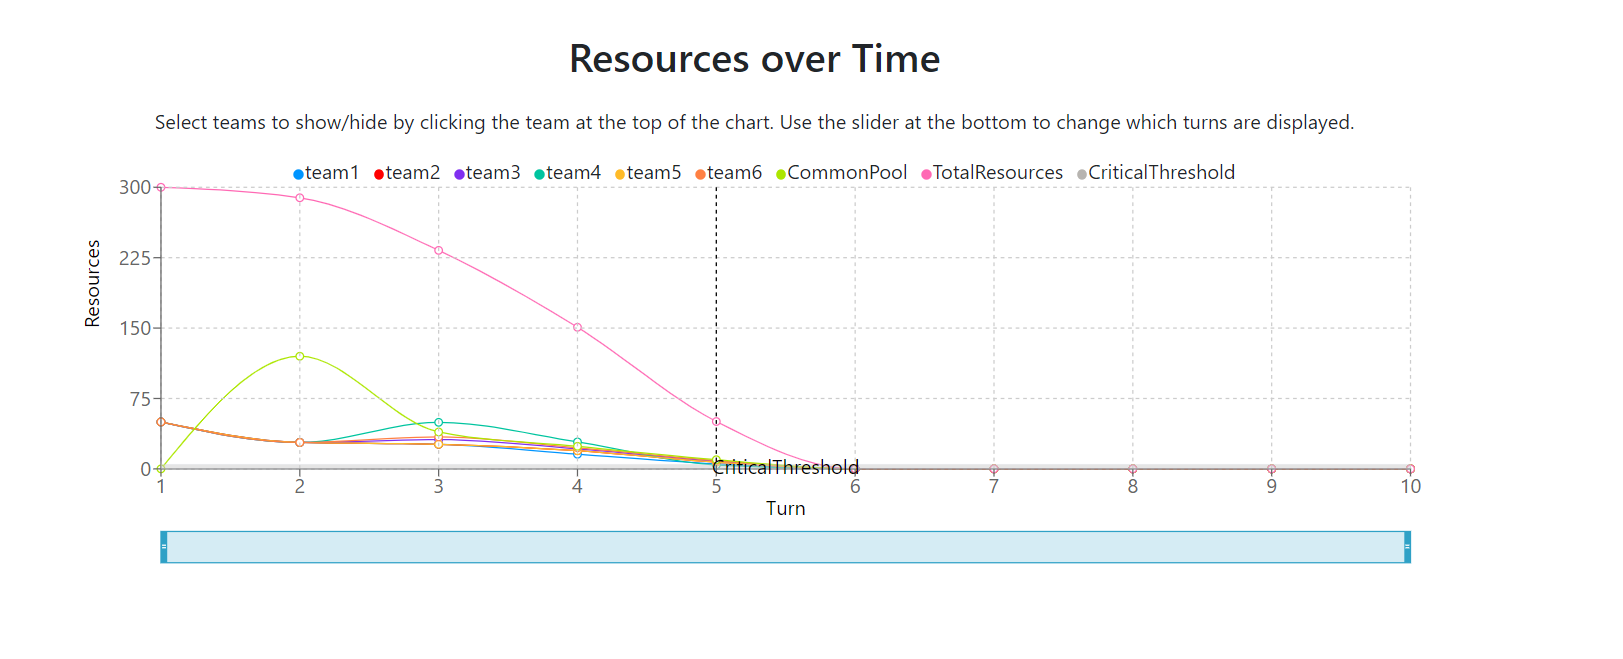
\includegraphics[width=0.7\textwidth]{images/altruist sim.png}
    \caption{Altruist simulation}
    \label{fig:  altruist sim}
\end{figure}
     \documentclass{article}

\usepackage[legalpaper, potrait, margin=1in]{geometry}
\usepackage[utf8]{inputenc}
\usepackage{gensymb}
\usepackage{graphicx}
\usepackage{float}
\usepackage{color,soul}
\usepackage[dvipsnames]{xcolor}
\usepackage{float}
\usepackage{array}
\usepackage{arydshln}
\usepackage{amsthm}
\usepackage{adjustbox}
\newtheorem{definition}{Definition}
\setlength\dashlinedash{0.2pt}
\setlength\dashlinegap{1.5pt}
\setlength\arrayrulewidth{0.3pt}
 
 \usepackage[linesnumbered,ruled,vlined]{algorithm2e}


 
 

\newenvironment{conditions}
  {\par\vspace{\abovedisplayskip}\noindent\begin{tabular}{>{$}l<{$} @{${}={}$} l}}
  {\end{tabular}\par\vspace{\belowdisplayskip}}


\title{Team 3: Pittstop Agent Strategy}

\begin{document}

\maketitle

\section{Introduction}

Team 3 was interested in the parallels between this project and human societies. We wanted to build an agent that was flexible enough to mimic the diverse personality traits of ordinary citizens, as well leaders in governments around the world.

Section~\ref{sec:overall_strat} discusses the foundation of parameters and methods the team wrote in its approach towards building the agent. Section~\ref{section_func_team3} details how the team used this foundation to implement the required functionality of the agent (i.e. roles, voting, prediction, gifting, foraging) in a way that is compatible with our goal of flexibility, without compromising efficiency or intelligence. Section~\ref{sec:team3_simulation} then elaborates on game simulations, in which the team decided to anthropomorphize the agent by modelling it after three famous historical and political personalities. Simulations consisting of different permutations of these personalities reveal interesting conclusions about the performance of the archipelago. Finally, Section~\ref{sec:management} concludes our report with information about project management.

\section{Overall Agent Strategy}
\label{sec:overall_strat}

\subsection{Overview}
\label{sec:overview}


The agent was created by first a set of high-level parameters, most of which were used as scaling factors throughout the code base of the agent, and some as Boolean values that turn on or off specific behaviours. These parameters hence govern the agents interactions with the rest of the game. The effect of each parameter on the behaviour of the agent is summarized in Table~\ref{tab:team3:parameter_effects}. \\


\begin{center}
    
\begin{table}[H]
\centering
\begin{tabular}{l|l}
\textbf{Parameters} & \textbf{Description}  \\ 
\hline
\texttt{equity}                       & controls the allocation distribution of resources amongst islands              \\ \hdashline
\texttt{resourceSkew}                 & factor to adjust resource allocation based on trust             \\ \hdashline
\texttt{complianceLevel}              & quantifies how often the agent cheata during the game             \\ \hdashline
\texttt{saveCriticalIsland}           & if True, our agent will try to save any critical island             \\ \hdashline
\texttt{selfishness}                  & quantifies how selfish our agent is (e.g. in the context of gifts)             \\ \hdashline
\texttt{riskFactor}                   & quantifies how much risk our agent is willing to take        \\ \hdashline
\texttt{friendliness}                 & quantifies how friendly we will be during agent interactions            \\ \hdashline
\texttt{sensitivity}                  & quantifies how sensitive the agent will be to external changes            \\ \hdashline
\texttt{giftInflationPercentage}      & factor to adjust when gift requests are made to other islands             \\ \hdashline
\texttt{advType}                      & enables the agent to exploit institutional powers when elected in a role    \\ \hdashline
\texttt{controlLoop}                  & boolean to enable the feedback loop for the agent       
\end{tabular}
\caption{List of global parameters that dictate our agent strategy.}
\label{tab:team3:parameter_effects}
\end{table}
\end{center}

\subsection{Core functions}

Based on these parameters, we also wrote a set of core functions which would be useful to all variations of the agent. These functions implement Opinion Formation and Compliance Calculation.


\subsubsection*{Opinion Formation} \label{section_opinion_formation}
In a game where there can be up to n-agents, \textit{opinion formation} allows our agent to quantitatively assess the behaviour of the others based on previous interactions. %The agent uses this information in the form of \textit{trust decision-making} to reduce uncertainties and ultimately maximise its returns during any activity. 
In our implementation, we use a \texttt{trustScore} map to keep track of the agent's trust in (n-1)-agents. This map is used in combination with other pre-configured parameters to make strategic decisions during a turn. 
Trust takes a score between 0 (lowest) and 100 (highest). At the beginning of the game, all trust scores are initialised at 50, representing a neutral opinion. In our implementation, the trust scores can change during the following game activities:

\begin{itemize}
    \item Gifting: When our agent receives gift offers (after requesting gifts) and actual gift amount(s) received.
    \item Role Evaluations: When our agent evaluates the performance of the President, the Speaker and the Judge based on their respective roles and responsibilities.
    \item Sanctions: When we receive the broadcast of sanction from the Judge outlining the sanctions placed for that turn.
\end{itemize}

%This mean that the more turns there are in a game, the more variation one will observe in the trust scores. They provide an effective source of perceived opinion for the agent to intelligently devise and choose a strategy in a given situation with limited external information. 

At every turn of the game, the agent will participate in multiple activities and hence, it would be counter-intuitive if the agent directly updated the \texttt{trustScore} map otherwise only the last score change would be retained. We thus implemented a local cache, \texttt{trustMapAgg}, to keep track of all trust score updates made during agent activities for that turn. 

In the following turn, the \texttt{trustScore} map is updated by averaging all cached trust score changes for each agent in play. This allows the agent to progressively accumulate knowledge while still forming independent opinions from the results of the activities in each turn. Trust scores are also bounded between 0 and 100 for consistency. The process (for a single turn) is summarized in Figure~\ref{fig:trust_scores}.\\

\begin{figure}[H] 
\centering
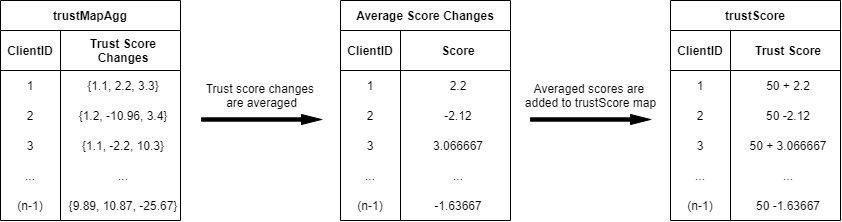
\includegraphics[width=0.75\textwidth]{figures/TrustScores.jpg}
\caption{Diagram showing the series of changes to trust scores during a single turn.}
\label{fig:trust_scores}
\end{figure}

%The \texttt{trustScore}  For example, when our island is elected as a Judge, the agent will rely upon these trust scores to determine which islands to pardon. This allows the agent to facilitate trust and forgiveness within the same framework.

\subsubsection*{Compliance Calculation}
Compliance Calculation determines at what point of the game it is most strategic to cheat. At every turn we calculate the \texttt{compliance} for the next turn\footnote{Note that \texttt{compliance} is how much our agent should comply at a given turn, while \texttt{complianceLevel} is how much our agent should comply during the entire game.}. The compliance calculation is based on the following principles:
\begin{enumerate}
    \item Every time we are caught, \texttt{compliance} is reset to 1.
    \item The more our agent is caught, the less it should cheat.
    \item If our agent has not been caught cheating for an infinite amount of turns, $\texttt{compliance}=\texttt{complianceLevel}$.
    \item The more our agent is caught, the longer it should take \texttt{compliance} to converge to \texttt{complianceLevel}.
\end{enumerate}

Those principles were converted into Equation~\ref{team3:eq:compliance}, shown here below:

\begin{equation}
    c(t,n)=\texttt{complianceLevel}+(1-\texttt{complianceLevel})\times e^{\frac{-t}{n+1}} \label{team3:eq:compliance}
\end{equation}

where:
\begin{conditions}
 c     &  \textttt{compliance} at a given turn \\
 t     &  time since the agent was last caught by a Judge (in number of turns) \\
 n    &  number of times the agent has been caught since the game started \\   
 \texttt{complianceLevel} &  target compliance - global parameters (see Table~\ref{tab:team3:parameter_effects})
\end{conditions}

Figure~\ref{fig:compliance_decay} illustrates how compliance decays based on the number of times caught. 

\begin{figure}[H] 
\centering
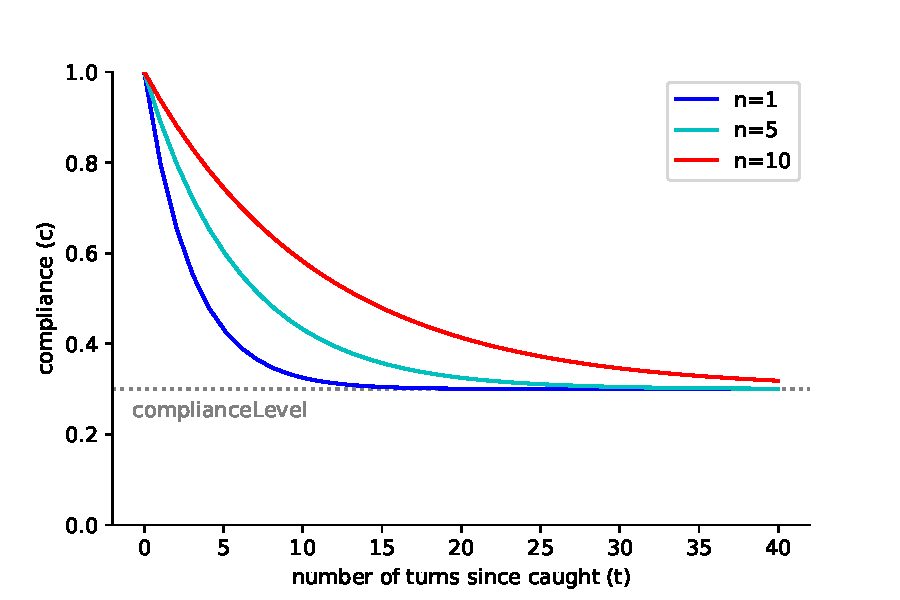
\includegraphics[width=0.4\textwidth]{figures/compliance_graph.pdf}
\caption{Compliance decay over several turns with $\texttt{complianceLevel}=0.3$.}
\label{fig:compliance_decay}
\end{figure} 

The agent, in various functions described in the following section, then decides whether or not to cheat by generating a random real number in $[0,1]$ and checking if it is lower than \texttt{compliance}.

% \begin{center}
%     \text{Let $X$ be a random number between 0 and 1,}
% \end{center}
% \begin{equation}
%   i.e.  X \sim U( [0,1]).
% \end{equation}

% \begin{equation}
%     if \; \texttt{compliance} < X \rightarrow \; cheat
%     \label{eq:should_I_cheat}
% \end{equation}

\subsubsection{Common State Variables}
In addition to the global parameters, a number of variables were also created to track the current state of the agent. These are accessed and updated by most functions throughout the agent's code base. 
\begin{itemize}
\item Gifting history
\item Trust scores for each island 
\item Performance score of each island for positions of power (i.e. the Speaker, Judge, President)
\item Number of times sanctioned
\item Cached information from IIGO (e.g. sanctions, monitoring outcomes and taxation/allocation)
\end{itemize}

\section{Implementation of agent-specific functions}
\label{section_func_team3}

This section covers how we implemented functions for each of the expected behaviours of the agent, as well as details of how they are affected by parameter changes.

\subsection{Voting}

\subsubsection{Voting for Rules}
Our rules are stored in the form of matrices, which opens up to our agent the geometric analysis of linear algebra. We observe that each rule matrix requires a number of inputs. These inputs may be considered to form $n-dimensional$ space. \\
As explained in Section~\ref{dynamics} below, our dynamics package is able to analyse these n-dimensional spaces and calculate whether a particular rule pushes us further from compliance or moves us towards a compliant position in this $n-dimensional$ space. Depending on whether the proposed rule brings us closer to compliance or not, we chose to vote for or against it.

\subsubsection{Voting for Elections}
At the end of each session of the IIGO, all islands need to submit votes for their preferences for the next Speaker, Judge and President. Since the vote is implemented using a Borda Count, teams are required to submit an ordered list of islands, ranked according to preference. 

We implemented voting by evaluating the performance of each island that held the positions of Speaker, Judge and President at the end of each IIGO session. Evaluations are performed using heuristics. Islands are ranked for each role based on the report from the accountability cycle and our interaction with the role during the turn. For example, if the Speaker chose the rule we suggested, they would have a better evaluation. However, if we get a smaller than requested allocation from the President, we would rank the island occupying the role lower.

\subsection{Environment}

\subsubsection{Foraging}
Foraging for our agent was implemented to maximise the return while maintaining a risk proportional to the \textttt{riskFactor} parameter. To achieve this, we use foraging results from previous turn from our island and the ones shared by other islands in  IIFO.
Our foraging strategy decision making ensures we are not in a critical state if foraging does not turn profitable.

At every turn, we follow the following strategy:

\begin{enumerate}
    \item Determine maximum foraging investment amount amount using the \textttt{riskFactor} parameter, our current resources and our estimation of the critical threshold.
    \item Set the maximum foraging investment amount based on our current resources and the minimum leftover resources amount.
    \item Compute the expected return of investment of both foraging techniques, hunting and fishing, using the stored history of past foraging returns. 
    \item If one foraging technique has a positive expected return, we compute a decay factor to adjust our investment based on what islands have chosen to forage in the last turn and how many dears/fishes were caught. This ensures that we do not hunt when the population is too low or that a lot of other islands are foraging with us.
    \item If no foraging technique is expected to be profitable, we only invest a small amount to get additional information in the next rounds and we don't take unnecessary risks.  
    \item The final amount we decide to forage is scaled by the risk factor parameter.
\end{enumerate}

This foraging decision making algorithm proved to be efficient and produces stable positive returns at different risk levels for our agent.

\subsubsection{Disaster Prediction}

Our agent predicts disaster using a combination of our own estimation of the disasters distribution and predictions from other teams.

Our estimation is obtained by computing the mean and variance of the coordinates, the magnitudes and the number of turns between past disasters. The variance is used to specify the confidence we have in our own prediction.

Other island's predictions are weighted based on their forecasting ability obtained by analysing their history of predictions of past disasters, the confidence they have in their own predictions as well as how much we trust them.

At each turn, we share our predictions with alive islands and store the ones from other teams. When a disaster occurs, we log this information to determine forecasting abilities of other islands.

\subsection{Trade}

The gifting session described provides four major phases for our agent to take part in. Trade is a two-way interaction and as per game sequence, it is the first opportunity (in every turn) to formulate an opinion.

\subsubsection{Gift Requests}
Our gift requests depend on 2 main parameters in our agent strategy, \texttt{giftInflationPercentage} and \texttt{riskFactor}, along with the \texttt{trustScore} map that we have built based on opinion formation of the other island. Essentially, we cover the risk that we do not get resources from the islands that we do not trust as much with what we get from islands that we do trust. Additionally, we do not request any gifts from critical islands in order to help them survive. \\

At every turn, we follow the following strategy:

\begin{enumerate}
    \item The resources our islands plans to ask for in gifts is calculated by finding the different between the \texttt{initialResourcesAtStartOfGame} and our \texttt{localPool}.
    \item If we actually need resources, we inflate the total requests that we make to account for differences in gifts we might actually receive. Otherwise, if do not actually need resources, we just request a percentage of \texttt{initialResourcesAtStartOfGame} for later opinion formation.
    \item We find the number of alive islands in the game and calculate the average amount of resources we will be requesting from each of them based on our total number of resources we wanted in the previous step.
    \item If an island is critical or dead, we do not request any gifts from them. For all other islands, we use the average request amount and adjust it according to \texttt{trustScore} of the island raised to the power of our island's \texttt{riskFactor}.
\end{enumerate}

\subsubsection{Gift Offers}
We make gift offers based on the other islands' gift requests, their respective \textt{trustScores}, and some of our agent's parameters such as \texttt{friendliness} and \texttt{selfishness}. However, if our island is critical, we do not many make any offers so that we can stay alive, but if our island's local pool resources are less than 10\% of \texttt{initialResourcesAtStartOfGame}, we still make a $0.01$ amount of gift offer to all alive islands. Our main strategy is to give as many gifts to the islands to maintain a good relationship with them.\\

In all other circumstances, we process the \texttt{receivedRequests} in the following manner:

\begin{enumerate}
    \item We use a sigmoid function to distribute and normalise the requests we receive from other islands based on their trustScore. More specifically, we use the following equation:
    \begin{equation}
    sigmoid = \frac{1}{1+e^{-0.1*(trustScore[island]-50)}}
    \end{equation}
    and normalise it so that the number is between 0 to 100, and then multiply it with the original request to scale the amount we are thinking of offering them. In this way, we offer less to islands that we trust less and more to islands we trust more.
    \item Calculate our gift budget based on \(\texttt{localPool}*(1-\texttt{selfishness}/2)\).
    \item Rank the islands based on their trust score in descending order.
    \item Allocate the gift offers starting from the most trustworthy islands onwards, until we run out of our gift budget.
\end{enumerate}
\\
Lastly, when we actually send the gifts to other islands at the end of each turn, we inflate our gift offers to improve other islands' opinion of us.

\subsubsection{Gift Responses}
We accept all amounts of gifts that the other islands offer us. The only exception to this is when the offering island is critical, then we do not take any of their offered amount in an attempt to conserve their resources as much as possible and increase their chances of survival as part of the common risk dilemma.

\subsubsection{Updating Gift History}
We use this section of gifting to do some opinion formation of other teams and more specifically update our \texttt{trustScore} map. If our offered gifts are declined or ignored with the reasons \texttt{DeclinedDontLikeYou} or \texttt{Ignored}, then we decrease that island's trust score by 5 and 2.5 respectively. When we actually receive our gifts, we compare the received amount to what we originally requested from an island, and use the difference to increase their trust score if they gave us more than we asked for or decrease it (with the exception of if the island is critical) if they gave us less.

\subsection{Taxation and Allocation}
%TODO: might need to move this for better organisation
\subsubsection*{Paying Our Taxation Amount}
Our taxation paying system has the similar aim as our President's tax allocation system. It aims to ensure that common pool has enough resources to survive the upcoming the disasters as well as run the next IIGO session. This is done based on the main assumption that each islands would probably pay proportionately to the trust that our agent has on them as well as others having the same aim as the agent's. This algorithm depends on \texttt{selfishness} and \texttt{riskFactor}.\\

At every turn, we follow the following strategy:

\begin{enumerate}
    \item Minimum resources that common pool should be is calculated based on the predicted disasters incoming as well as the cost of running IIGO.
    \item Distribute the share of the payment based on the trust on them, with the agent's own trust being represented by 1-\texttt{selfishness}.
    \item Calculate the minimum amount of resources the agent should have, this depends on the \texttt{riskfactor}. 
    \item Ensure that the taxation amount will not put the agent below the minimum resources. 
    \item Depending on our compliance level, if our calculated amount is lower than our given taxation, we will increase it accordingly.
\end{enumerate}


\subsection{Positions of Power}

\subsubsection{Judge}

% The judicial branch references the functionalities an island can implement if they are elected as the Judge. 
The overall strategy for our island as the Judge was to enforce stricter laws to encourage more obedience (in the future) from the other agents while respecting the power, permission and obligation paradigms. 

\subsubsection*{Inspect History}
To respect the role of the Judge, our client performs the inspection as per base Judge implementation (i.e. evaluates if rules were followed by all islands) with the exception that our and other highly trusted islands (whose trust score is above 80) are exempted from all evaluations. A false evaluation map indicating full compliance with rules is produced for these cases and a correct evaluation is produced for all the other islands. 

% \subsubsection*{Rule Violation Severity}
% Our agent does not override these severities because we did not have sufficient opinion formation on rules to enforce harsher penalties. Instead, emphasis was placed on changing the sanction thresholds.

\subsubsection*{Sanction Thresholds}
Our agent has set a linear scaling for all sanction tiers, which makes it easier than the default sanction thresholds to fall in higher sanction tiers. The aim is to enforce harsher penalties that achieves the overall objective of the Judge client.

\begin{table}[htb]
    \centering
    \begin{tabular}{|c|c c|}
    \hline
    \textbf{Sanction Tiers}  & \textbf{Default} & \textbf{Our Island} \\ \hline
\textbf{Tier 1} & 1    & 1    \\
\textbf{Tier 2} & 5    & 6  \\
\textbf{Tier 3} & 10   & 11 \\
\textbf{Tier 4} & 20   & 16   \\
\textbf{Tier 5} & 30   & 21  \\
    \hline
\end{tabular}
\caption{Our agent's sanction thresholds compared to the default thresholds.}
\label{table:sanction_thresholds}
\end{table}

\subsubsection*{Pardon Islands}

Our Judge pardons islands based on if their trust score is greater than or equal to 50 (our neutral trust score value) and our agent's \texttt{friendliness} is set to more than 0.5. We also pardon our own agent's sanctions. This allows the agent to forgive other islands as part of the trust-forgiveness framework.

\subsubsection*{Historical Retribution}

Our Judge checks if the \texttt{judge\_historical\_retribution\_permission} rule is in play in the game, and if it is, we disable historical retribution so that we follow the rule. Otherwise, we break the rule and enable historical retribution, so that we can inspect more of the other island's behaviour in previous turns in order to sanction them, etc. Again, this helps to fulfill the overall objective of our Judge.

\subsubsection{President}
The President has four main responsibilities:

\begin{enumerate}
    \item Set the required tax amount for each island.
    \item Evaluate the allocation requests from each island, and set the allocated resource amount from the common pool.
    \item Decide which rule to be voted on.
    %\item Monitor the Speaker, and call an election if necessary.
\end{enumerate}

For each of those responsibilities, we have created our own strategy based on the parameters shown in Table \ref{tab:team3:parameter_effects}.

\subsubsection*{Taxation}
\subsubsection*{Setting Taxation Amount}
Our allocation of taxation amount depends on three parameter \texttt{equity}, \texttt{selfishness}, and \texttt{resourceSkew}. The algorithm aims to make sure that common pool has enough resources to survive the incoming disasters as well as enough for IIGO to run in the next turn.\\\\
At every turn, we follow the following strategy:

\begin{enumerate}
    \item From the reported resources, each island's actual resources are predicted based on their trust score.
    \item Minimum resources that common pool should be is calculated based on the predicted disasters incoming as well as the cost of running IIGO.
    \item The amount is first distributed equally, then is adjusted based on their resources they have. The extends of adjustment depends on the \texttt{equity} parameter.
    \item We reduce the amount of our own tax based on our \texttt{selfishness}, while others remains the same.
\end{enumerate}

\subsubsection*{Request Allocation}
Our request allocation depends on 4 parameters: \texttt{selfishness}, \texttt{equity}, \texttt{saveCriticalIslands} and \texttt{resourceSkew}. It aims to, in order of priority, (1) ensure there will be enough in the common pool to survive a disaster, (2) maximise our own survival\footnote{This refers to how much we prioritize ourselves over other islands decided based on \texttt{selfishness}.}, (3) save any island that is \texttt{critical}\footnote{This only the case if \texttt{saveCriticalIslands} is set to \texttt{True}.} and (4) be equitable\footnote{This depends on the value of the \texttt{equity} parameter.}. \\

At every turn, we follow the following strategy:

\begin{enumerate}
    \item Obtain allocation requests, discard outliers, and compute average request
    \item Calculate the allocated resources for each island based on the computed average and their request. The allocated resource is weighted by  \texttt{trustScore} (if we trust them, we will give them what they requested), \texttt{equity} (if our island values equity, everyone will receive average allocations), and \texttt{selfishness} (if we are selfish we will allocate ourselves more than the other islands)\footnote{If our agent is set to save \texttt{critical} island, this is also taken into account.}. 
    \item Check if after allocating resources, the common pool would still have the predicted minimum amount of resources required to survive a disaster in the upcoming turn. If not, adjust allocation to fulfill this requirement. 
\end{enumerate}

\subsubsection*{Rule Selection}
The matrix representation of rules opened up a huge amount of geometric analysis to us, which we have encapsulated in a package we call \emph{dynamics}. The dynamics package provides us with the tools required to analyse rule matrices, by converting them into geometric subspace, we are able to quantitatively measure how beneficial a particular rule will be to us and propose or vote on that rule using that information. For the algorithm that enables this behaviour is covered by Section \ref{dynamics}.

%\subsubsection*{Speaker Monitoring and Election}
%The decision to monitor and announcement of the monitoring outcome follows that of the base client implementation (i.e. always monitor the Speaker and always declare the true monitoring outcome). \\
%The election of speaker is only called if monitoring was performed and indicated foul play or if the current speaker has held the position for more than 3 turns. However, the speaker selected when we are president will always be the island we trust most.
%If the agent is using the differing personalities (section \ref{section_agent_personalities}), then the behaviours for monitoring and elections may be overridden to suit the intentions of the persona.

\subsubsection{Speaker}
We found it quite difficult to integrate our persona's and strategy. This is mainly because it is almost always in our best interest to follow the constitutional rules as a speaker.\\

\subsection{Dynamics}
\label{dynamics}
Dynamics is our rule analysis package. Since in our archipelago rules are represented by matrices, we are able to perform linear algebra driven geometric analysis. This analysis is based on the idea that since each rule matrix requires a set of input variables, these variables can be considered to construct an $n-dimensional$ space. The rule-matrices can then be considered to be operations on this $n-dimensional$ space, furthermore we can use the matrix and supporting information to define a subspace of the $n-dimensional$ space which is compliant. \\

We can then calculate the distance between our position (our agent's values for the variables required for the rule) and the subspace via Algorithm~\ref{algo:dynDistance}.

\begin{algorithm}[H]
\DontPrintSemicolon % Some LaTeX compilers require you to use \dontprintsemicolon instead
\KwIn{RuleMatrix (matrix)}
\KwOut{distance (float64)}
 \If{$matrix.dims$ \textbf{is} $not valid$} {
   \textbf{return} \textit{-1}\;
 }
 
 \Else{
 \textbf{smallestDistance} $= \infty$ \;
 
 \While{$RuleMatrix.hasMoreRows$}{
 \textbf{Get} $nextRow$\;
 \textbf{Convert} $nextRow$ \textbf{into} $hyperplane$\;
 \textbf{Calculate} $singleDistance$ \textbf{between} $ourPosition$ \textbf{and} $hyperplane$\; 
 \If{$singleDistance < smallestDistance$}{
    \textbf{set} $smallestDistance = singleDistance$
 }
 }
\textbf{return} $smallestDistance$
 }
\caption{Dynamics - Calculate distance between our island's position and the rule}
\label{algo:dynDistance}
\end{algorithm}

This algorithm provides us with an important metric when it comes to analysing rules, how far away our position is from the compliant subspace of the rule. Assuming monotonicity in the subspace, we can interpret this distance as the effort required to reach compliance, and therefore a rule whose compliant subspace is closer to us than another rule, would be preferred by our agent. \\

\subsection{Adv}
We have created one final package as part of our agent strategy, which we call \emph{adv}. This package was designed mainly to attempt to probe and attempt to exploit IIGO. It provided our agent with overrides for our normal functions, that took into account the particular workings of IIGO and how to probe and exploit them.\\

\subsubsection{Malice}
Malice is an \emph{adv} that possesses the the tools required to exploit IIGO and stay in power indefinitely. Furthermore, when this \emph{adv} is in the position of the President, it will tax the other islands their entire resource reports and pay itself huge allocations. We use \emph{Malice} to model the abilities of an acutely intelligent agent, which knows the exact loopholes of government and has the will to exploit them.

\subsubsection{Target}
Target is an \emph{adv} which we built almost entirely out of interest. It has the same capabilities as Malice but only ever uses them against a particular target island which is configurable. For example, when any other island is in a position of power \emph{Target} behaves as normal, but when the target island is in power \emph{Target} attempts to gain power via elections and pushes out the other island using knowledge of IIGO's accountability cycle. We chose not to deploy \emph{Target} in simulations since such a model would essentially be a scaled version of \emph{Malice} an adv for which we already had results.

\section{Simulations and Analysis}
\label{sec:team3_simulation}

The number of parameters, each of which can be a real number in $[0,1]$, gave us a large degree of freedom for analysis. To make the discussion more focused, we selected three sets of parameters governing the behaviour of three very different types of agents. Running simulations with permutations of these agent personalities led to some interesting observations about governance, risk, and the extent of selfishness required for the archipelago to thrive. Simulations were performed in the same game environment described in Section 15, except with the maximum number of turns reduced to 51. The analysis of our simulations uses the same metrics described in Section~\ref{subsec:Simulations:baseline:num_metrics}.


\subsection{Agent Personalities} 
\label{section_agent_personalities}

We created three vastly different agent strategies by tweaking all agent parameters by small amounts, and experimenting with more significant changes to \texttt{riskFactor}, \texttt{complianceLevel}, \texttt{advType} and \texttt{selfishness}.

\subsubsection{Gandhi}
The \textit{Gandhi} agent behaves like an altruist - with low risk and selfishness factors, and a perfect compliance level.

\subsubsection{Putin and \textit{Benevolent} Putin}
The \textit{Putin} agent is built to be a tyrannical dictator, with high risk, maximum selfishness and a low compliance level. It never contributes to the common pool. The Putin agent also has its \textttt{adv} parameter set to \textit{Malice}. This setting activates a new set of methods that abuse the powers of the Speaker, Judge and President respectively.  Once elected into a position of power, the Putin agent abuses the accountability and transfer-of-power cycles to take over the IIGO. As President, it increases taxation and steals the entire common pool for itself, thereby shutting the IIGO down and killing all other islands.

 \textit{Benevolent} Putin is built to be less extreme. It is less harsh when in power, and most importantly does not take control of the common pool - IIGO is therefore able to continue for the entire game. The Benevolent Putin is a more realistic representation of authoritarian regimes around the world, letting enough resources for others to barely survive.

\subsubsection{Ardern}
The \textit{Ardern} agent is built to mimic reasonable behaviour, in positions of power and otherwise. With moderate risk and selfishness factors, as well as a high (but not perfect) compliance level, it behaves truthfully and contributes to common interests, unless in critical condition (i.e. in danger of dying within the next few turns). We use this agent when running simulations with those of other teams.

\subsection{Experiments}

We performed multiple experiments, with archipelagos of different permutations of the above agents. The results of some of the more interesting ones are presented in the table below.

\newcolumntype{L}{>{\centering\arraybackslash}m{2.5cm}}

\begin {table} [h]
\begin{center}
\begin{adjustbox}{max width=1.1\textwidth,center}
\begin{tabular}{|p{0.21\linewidth}||L|L|c|L|c|c|}
    \hline
    \textbf{Agent Config} & \textbf{Archipelago Survivability} & \textbf{First Island death} & \textbf{Gini index} & \textbf{Disasters Survived} & \textbf{ADDM} & \textbf{AFS} \\ \hline \hline
    \textbf{6 Gandhi} & 51  & 51 & 0.04 & 10 & 175.08 & 1.71 \\ \hline
    \textbf{6 Arden} & 51  & 51 & 0.10 & 10 & 112.743 & 1.51 \\ \hline
    \textbf{6 Benevolent Putin} & 51  & 36 & 0.54 & 10 & 167.095 & 1.58 \\ \hline
    \textbf{6 Putin} & 51  & 25.7 & 0.20 & 10 & 0.00 & 1.24 \\ \hline
    \textbf{1 Gandhi, 5 Ardern} & 51  & 51 & 0.12 & 10 & 123.636 & 1.54 \\ \hline
    \textbf{3 Gandhi, 3 Ardern} & 51 & 51 & 0.09 & 10 & 153.22 & 1.55 \\ \hline
    \textbf{1 Benevolent Putin, 5 Gandhi}  & 51 & 51 & 0.38 & 10 & 209.90 & 11.41  \\ \hline
    \textbf{1 Benevolent Putin, 5 Arden} & 51  & 40.4 & 0.53 & 10 & 144.24 & 3.12 \\ \hline
    \textbf{3 Putin, 3 Ardern} & 51 & 14.4 & 0.68 & 10 & 87.8275 & 2.66 \\ \hline
    \textbf{3 Putin, 3 Gandhi} & 51 & 16.9 & 0.61 & 10 & 103.04 & 5.73\\ \hline
\end{tabular}
\end{adjustbox}
\end{center}
\label{tab:team3:all_experiment_results}
\caption{Simulation results and metric analysis for different agent configurations.}
\end{table}

\subsection{Analysis}

Trends across the experiments support the following conclusions:

\subsubsection{Relationship between long-term Collective Risk Dilemma and Foraging Efficiency}
The first general trend we observed was that the AFS rises in tandem with ADDM. This initially seemed paradoxical - for the ADDM to rise, islands must have contributed more to the common pool. Yet, despite parting with more of their resources, they were able to make better foraging decisions, explaining the rise in AFS. This is due to the fact that a healthier common pool reduces the impact of disasters on islands, leaving them with more resources for foraging, and that allocations from the common pool are used to rescue islands from critical states -- obviously, islands that are alive are likely to make better foraging decisions than those that are not. This relationship is further explored in Section \ref{subsec:Simulations:no-iigo:conclusion}.

\subsubsection{The IIGO, even if abused, improves archipelago performance}
The Putin agent was written as an experiment of the most selfish and evil form of governance possible. Putin simulations are consistently the worst across all experiments conducted, as the Putin agent shuts the IIGO down once it takes power. The effect of this is explored in Section \ref{sec:ResultsAndEval:no-iigo}. 

The Benevolent Putin, on the other hand, attempts to be a little more devious. The persona contributes enough via tax to the common pool to keep IIGO running, and then continues to pay enough tax to ensure that disasters are mitigated. All the while this version of Putin still abuses IIGO, allocating itself far more allocation than other islands, but keeps others alive. This leads to effectively a benevolent dictatorship. However, it is worth noting that all metrics indicate a better outcome for the archipelago in this case.

\subsubsection{Altruistic agents improve archipelago performance}

Interestingly, the best performing archipelago - across all six metrics - was the one that consisted of six Gandhi agents. This archipelago had a remarkably low Gini Index of just 0.04, almost ten times lower than the baseline simulation result presented in baseline simulation section. The fair taxation system and selflessness of the agents also ensured a healthy common pool which was able to mitigate disaster damage, which explains why this archipelago had the highest ADDM metric (and consequently, as per the analysis above, the second highest AFS metric as well).

In fact, every simulation that replaced Ardern agents with Gandhi ones, or increased the number of Gandhi agents, performed better than its counterpart. Gandhi agents consistently decrease the Gini Index and increase the ADDM of the archipelago, even when Putin/Benevolent Putin agents shut down or abuse the IIGO -- this can be attributed to the Gandhi agents giving more gifts to each other and contributing more to the common pool (before it is stolen). Clearly, the more prevalent altruistic behaviour is, the better the archipelago fares. 

% DW mate i saveed these in another file

\section{Project Management}
\label{sec:management}

The project management regarding Team 3 went through four major iterations, following closely with significant deadlines of the group-wide project. The four phases are summarised as follows, with Table~\ref{tab:phase_jobs} summarising the assignments that each team member had over the phases.

\begin {table} [h]
\begin{center}
\begin{adjustbox}{max width=1.1\textwidth,center}
\begin{tabular}{|c||c c c c|}
    \hline
    Name & Phase 1 - Research & Phase 2 - MVP & Phase 3 - Post MVP & Phase 4 - Finalised Agent\\ \hline \hline
    Preet & Research & Infra Rep & Infra Rep/Speaker & Post MVP Infra/Final Report \\ \hline
    Ezgi & Research & Design Rep & Design Rep/Judge & Post MVP Design/Final Report \\ \hline
    Noé & Research & Internal Design & President & Graphics/Final Report \\ \hline
    Tharusha & Research & Internal Design & President/Island Common & Island Refactoring/Fixing \\ \hline
    Ramon & Research & Infra Associate & President/Island General & Visualisation  \\ \hline
    Neelesh & Research & Infra Rep & President/Infra Rep & Post MVP Infra/Tuning \\ \hline
    Agrim & Research & Design Associate & Judge/Gifting & Simulation \\ \hline
    Victor & Research & Internal Design & Speaker/Environment & Simulation \\ \hline
    Nidhi & Research & Infra Associate & Judge/Gifting & Simulation \\ \hline
    Kunal & Research & Design Associate & Speaker/Voting/Environment & Simulation/Tuning \\ 
    \hline
\end{tabular}
\end{adjustbox}
\end{center}
\label{tab:phase_jobs}
\caption{Assignments for each team member over each phase.}
\end{table}

\subsection{Phase 1 - Research, Design and Reps }
With the commencement of the project, the immediate task was the delegation of roles between members of team 3. The first call of action was to decide who would be assigned as the design and infra reps. Once this was agreed, the initial plan was to divide the group up to focus on specific aspects of the lectures that were relevant to the project, with the aim to brainstorm some design ideas that could be brought up in the design meetings. Thereafter, the team had weekly meetings to discuss their findings and identify the areas that the concepts can be applied in the project.
\subsection{Phase 2 - MVP}
With design eventually underway and infrastructure also starting, the team was subdivided into 3 sub-teams: infra and design associates, whose task was to join the reps and assist in the respective developments, and an internal design team, whose task was to brainstorm and focus on the specific island itself. The initial design and infra MVP deadline was set, and with it the team was assigned the implementation of a 'base' version of the IIGO roles: President, Speaker and Judge. To effectively split the workload, the team was split into three sub-teams to implement the functions for these corresponding roles.

\subsection{Phase 3 - Post MVP and Agent Strategy}
Once the global MVP was finalised, and deadlines set for the internal island design, the required 'client' functions (expected functions of all islands) were listed and distributed amongst the team. The approach we took was for each of the Speaker, Judge and President role sub-teams (named Pelosi, Roberts, and Biden respectively) to take responsibility of designing the role specific functions, as well as nominating to take some client functions. This was managed via a Trello Kanban Board (Figure \ref{fig:post_mvp_trello}). Each team was required to analyse the requirements, design, corresponding behaviours, and document pseudo-code for each of their functions. This allowed for easy identification of an island 'common state' - a list of common variables and parameters which could be shared amongst the various functions. Once the pseudo-codes were finalised, each sub-team was tasked with the Golang implementation of their functions in the agent. Hence, the main implementation of the agent was therefore achieved in time for the internal agent deadline.

\subsection{Phase 4 - Finalising Agent}
Following the project-wide first agent-strategy deadline, there were 3 key areas for agent in which the team was reorganised:
\begin{itemize}
    \item Simulation - Testing of the agent strategy with different parameters and recording of interesting outcomes/behaviours.
    \item Parameter Tuning - tuning of the strategy's default parameters that create optimal behaviour for the general game and interaction with the other teams.
    \item Final Agent Report - structure and review of final agent strategy report
    \item Final Collective Report - structure and review of final collective report to be handed as a class
    \item Visualisation - joined the visualisation team to create output graphics
    \item Island Management - code cleanup, review of internal island strategy for final deadline
\end{itemize}
Every team member was also assigned responsibility contributing to the agent-strategy presentation content as well as the final report, writing up about their respective sections and allowing for a smooth finalisation to the agent-strategy.

\begin{figure}[H]
    \centering
    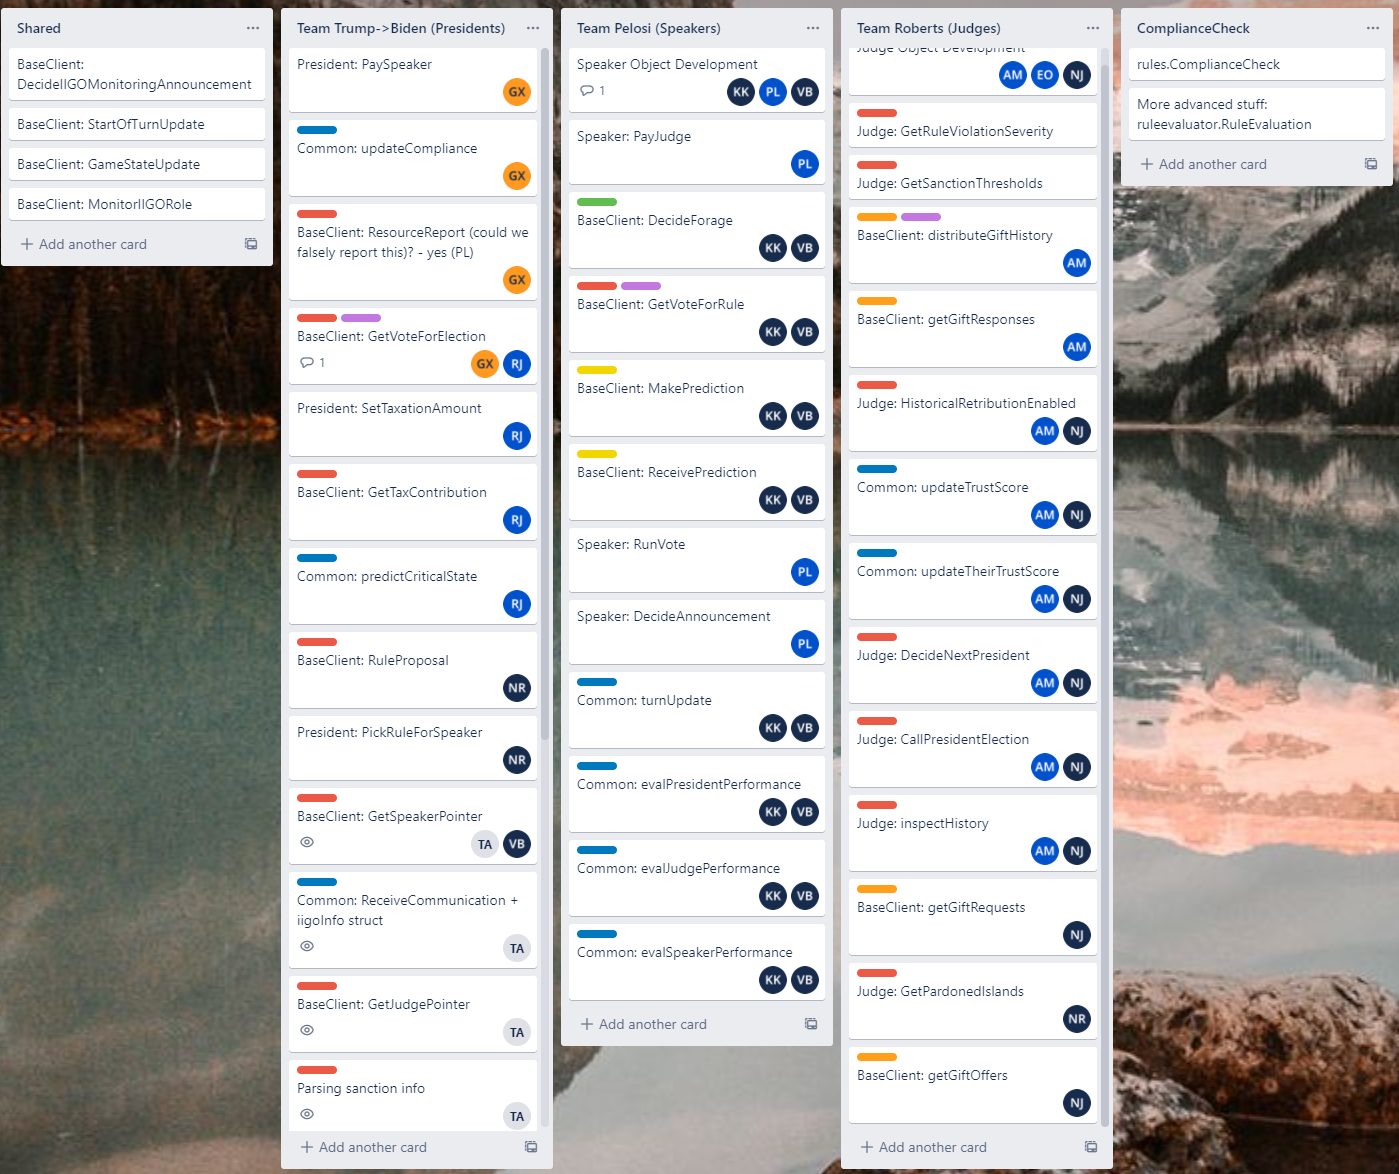
\includegraphics[width=\textwidth,height=\textheight,keepaspectratio]{figures/post_mvp_trello.png}
    \caption{Screenshot of post-MVP agent strategy kanban Board.}
    \label{fig:post_mvp_trello}
\end{figure}

\end{document}
    % \newcommand{\subsubsubsection}[1]{\paragraph{#1}\mbox{}\newline}
% \setcounter{secnumdepth}{4}
% \setcounter{tocdepth}{4}


%TODO: Please DO NOT RESOLVE the comments unless you are 100% sure everything related to the comment is resolved, as they can't be retrieved.
%TODO: VERY VERY IMPORTANT: talk to people in our group to make a decision on understanding of the "lack of variety"  that is shown in the comment on line 276 of this latex file. This will cause quite a few changes in the report but it is a very important concept to clarify to avoid burning ourselves. Read all the comments Mike made in the relevant sections first.
%TODO: VERY IMPORTANT: another potential self burn area. Clarify with Rudolfs about Ostrom's Principles after looking at all the comments Mike has made in that section.
%TODO: add in rule distance calculation explanation? It's kinda primitive though
%TODO: President by Andrzej, do talk about disaster prediction
%TODO: Toby to finish all foraging related stuff (IIFO and End of turn)
%TODO: add in the use of disaster prediction somewhere if we can?
%TODO: to finish IITO and gifting, sneak in disaster prediction if possible
%TODO: clear up all the TODO's scattered around in this latex file.


\chapter{Team 4 Agent Design}
Given that our team invested a lot of time in ensuring feature richness and stability of the infrastructure, we were left with a short time-frame for our agent's implementation and design. Therefore, at times we had to make decisions that guaranteed canny usability, rather than sophistication. For some actions, our agent relies on other teams' agents with different strengths to perform well. 

\section{Agent overview}
An agent uses the interface that is defined in the infrastructure. In order to define custom behaviours for our agent, we override or extend the base agent (baseclient.go) functions which implement the defined interface. The main idea we have for our agent is that it has internal fields that aid the decision-making process for the actions it performs. Of all the internal fields, we define internal parameters as information that describes the agent itself, namely \texttt{Greediness}, \texttt{Selfishness}, \texttt{Fairness}, \texttt{Collaboration} and \texttt{RiskTaking} factor, all of which have values between 0 and 1. And the agent stores observations, histories as well as other necessary information such as its trust in others. These fields will be further explained in the following text. %TODO: add in evolutionary economic theory background for agent personality

An agent can also be elected one or more roles inside the IIGO session. Each role has the power to perform role actions specified in the Roles section. These actions are implemented as functions in the code and they can be extended and overridden in the same fashion as in the base agent functions. Even though a role and an agent that is not elected a role (a commoner agent) are two separate structs, a commoner agent and a role have both read and write access to the internal fields of each other through pointers. In other words, an agent is always a commoner agent, and a commoner agent can be elected one or more role(s) at the same time.

\section{Opinion formation -- Trust}
\label{sec:team4:trust}
Trust is the score $[0..1]$, which represents the opinion of all the agents in the game. This metric helps our agent to make the decisions throughout the game based on how trustworthy, helpful or friendly we other agents were. This option about an island is formed based on three observations:
\begin{itemize}
    \item The gifts received from this island during the IITO sessions.
    \item The outcome of the monitoring of positions-of-power conducted as a part of the accountability cycle.
    \item The evaluation of IIGO actions history, only available to the Judge. This is further explained in Section~\ref{subsec:team4:judge}
\end{itemize}
Those observations allow the agent to quantitatively reason about both friendliness of other islands towards it, as well as whether they follow the rules in play.

The average trust is maintained at a value of $0.5$. That ensures that the trust is balanced throughout the game. It prevents the inflation of trust when all the islands decide to exchange gifts with the agent. Then, the number of resources gifted will be a deciding factor when updating the trust metrics.

Decisions made by our agent can be altered based on the trust score towards certain islands. For example, if the trust of an island is lower than a specified threshold, then the agent will not vote for this island in any elections. Similarly, if holding the role of Judge, will not choose to act upon its power to pardon the island with a low trust score.

On the other hand, if an agent holds a good opinion about an island, it may choose to act in favour of it. The island may expect to receive gifts from our agents, or be considered for an early pardon from a sanction.


\section{IIGO}
\subsection{Commoner Agent}
Within IIGO, each (commoner) agent first reports how many resources it has, this reporting behaviour is overridden by us. The president sets a taxation amount according to each agent's self-reported resources level and notifies each agent of the tax demanded. Each (commoner) agent sends a request for the resources it wants from the Common Pool (an allocation request) to the President. And after being granted the resources by the President, the agent takes them from the Common Pool. The actions concerning requesting and taking allocations are overridden by us. Due to a design decision, the action for taking allocations and paying tax do not happen within the IIGO session, it happens after all organisations are run, inside the \texttt{EndOfTurn} session.

\subsubsection{Report Resources}
When reporting the resources our agent has, We use a linear combination of some of the agent's internal fields, and weights (put inside an \texttt{importance} vector) we set for each of the chosen internal fields. The linear combination gives a scaling factor to scale (in this case to divide) the actual resources our agent has (as shown in \eqref{linear_comb}). The parameters used are \texttt{greediness}, \texttt{selfishness}, \texttt{fairness}, \texttt{collaboration}, \texttt{riskTaking} and trust in the current president (all values are between 0 and 1). The weights have real values. The fields with negative weights negatively impact the scaling factor and vice versa. The greater the absolute value of a weight, the bigger impact it has on the scaling factor.

\begin{equation}\label{linear_comb}
    \begin{bmatrix}
        w_{1}& w_{2}& w_{3}& w_{4}& w_{5}& w_{6}
    \end{bmatrix}
    \cdot
    \begin{bmatrix}
    Greediness \\ 
    Selfishness \\ 
    Fairness \\ 
    Collaboration \\ 
    RiskTaking \\
    TrustScore_{President}
    \end{bmatrix}
    = Scaling\:Factor
\end{equation}

The scaling factor is then compared to a preset threshold. If the scaling factor is greater, then the needed resources amount is divided by 
\begin{equation}
    [1 + (Scaling\:Factor - Preset\:Threshold)]
\end{equation} 
The threshold is there to make sure that the scaling factor is not applied all the time, as we don't want our agent to lie about the amount of its resources all the time.

\subsubsection{Paying Tax Contribution}
%write about this and the lying mechanics
The \texttt{GetTaxContribution()} function returns the amount an agent is paying in tax. Similar to resource reporting, the tax amount is modified by a scaling factor. When the scaling factor is greater than a preset threshold, the amount of tax paid is the tax demanded multiplied by: 
\begin{equation}
    [1 + (Scaling \: Factor - Preset \: Threshold)]
\end{equation}
, which is likely to happen when the \texttt{Collaboration} of our agent is defined to be high. In addition, the scaling factor is not applied when the tax demanded is more than $\frac{1}{5}$ of the agent's resources. This prevents the agent from generously giving out everything it has.

\subsubsection{Requesting Allocation}\label{subsubsection:CommonPoolResourceRequest()}
This is done in the \texttt{CommonPoolResourceRequest()} function. When requesting an allocation, our agent first decides what it needs. When the agent is not in a critical state, the needed resources are usually a multiple of the basic needs, namely the cost of living plus the critical threshold. This amount is decided so that the agent always takes more from the Common Pool than their definite expenses in the next turn. When in a critical state, the needed resources are a bigger multiple of the basic needs. Because the smaller multiple of basic needs when not critical made the agent critical, which indicates that the island needs to take more resources to not slowly drain away its own resources. In order to maintain the Common Pool, we also enforce that what our island needs must not exceed the amount of resources in the Common Pool divided by the number of agents alive. This is to avoid our agent monopolising the Common Pool resources based on just what it needs.

\subsection{President}
\label{subsec:team4:president}
%andrzej
Our agent implements a simple, rule-obeying President. %president also uses disaster prediction which is implemented. The confidence value is between 0 and 100% for each prediction.

% tax distribution 


% resource allocations
% tries to be fair. gives priority to critical islands. uses lowest amount first to ensure that the highest number of island is satisfied with common pool distribution

% speaker elections




\subsection{Judge}
\label{subsec:team4:judge}
The Judge implementation provided by our agent can be described as \emph{honest, but curious}. In other words, it follows the rules currently in play, and follows its obligations, however, it extracts the information exclusive to Judge to reason about other agents in the game. An example of such actions is explained in greater detail below in this Section.

The judiciary functions overloaded from the \texttt{basejudge} implementation are:
\begin{itemize}
    \item \texttt{InspectHistory}, which examines rule violations of all the agents.
    \item \texttt{GetPardonedIslands}, which considers reducing the sanctions for some agents at judges discretion.
    \item \texttt{CallPresidentElection}, which initialises \emph{transfer-of-power} of the executive branch.
\end{itemize}
An explanation of the implementation of those functions is presented below.

\subsubsection{IIGO history inspection}
\label{subsubsec:team4:judge:inspect_history}
In the basic implementation, a history of IIGO actions of all the agents is passed to the Judge for inspection, which could become grounds for introducing economic sanctions for non-rule-obeying players. 

Judge truthfully evaluates and reports the rule violations of each of the agents, just as the \texttt{basejudge}. However, it also extracts and saves the information about the private resource pools of all the agents, taxes they were expected to pay, as well as the actual amount paid to the common pool. Additionally, it stores the \texttt{LawfulnessRatio} of each agent, which can be written as:


\begin{equation}
    lawfulness_{i} = \frac{number\:of\:rules\:obeyed\:by\:the\:agent_{i}}{total\:number\:of\:rules\:inspected\:by\:the\:judge\:for\:agent_{i}}
\end{equation}

where $agent_{i}$ is denotes $i^{th}$ agent in the game.  

The \texttt{LawfulnessRatio} is then used to update our agents' trust towards other islands, thus influencing decisions in different parts of the game. 

\subsubsection{Consideration of pardons}
Compared to the \texttt{basejudge}, which does not grant any pardons and requires islands to pay economic sanctions in full, our implementation of the Judge allows for the pardoning of certain islands. We consider three parameters when deciding whether and the island could be pardoned:

\begin{enumerate}
    \item The severity of the sanction - only sanctions lower than specified severity level can be considered to be pardoned. This ensures that our Judge never pardons an island, who notoriously breaks the rules of the game and gets sanctioned for it.
    \item Time served on the sanction - the Judge will only remove the sanction if at least the specified number of turns has been served by the island. This still allows us to have a punishment for not obeying the rules but also ensures that an island can begin to contribute again earlier.
    \item Trust towards the island sanctioned - only islands, which are considered trustworthy by our agent can be pardoned. The threshold is tuned by an internal parameter of our agent.
\end{enumerate}

An island can be pardoned by our implementation of Judge only if they meet all three requirements presented above. 


\subsubsection{Presidential elections}
The \texttt{basejudge} implementation called an election every three turns, no matter how long the presidential term was. Our Judge implementation improves on that by calling an election only under two conditions:
\begin{enumerate}
    \item The term of the president has ended.
    \item The president did not fulfil its obligations and was dishonest while holding the executive office. It is decided based on the monitoring results coming from the accountability cycle.
\end{enumerate}

This implementation could be further improved to facilitate the \emph{trust} metrics, explained in Section~\ref{sec:team4:trust}. An example of such an improvement would be allowing the president to hold the office longer than its turn if he is most trustworthy according to our internal \emph{trust} metrics.

\subsection{Speaker}
Given the Speaker's role of deciding agendas and announcing the results of voting, the only viable customisation option in making our custom Speaker seemed to be via implementing corruption - in other words, rigging voting results. Other than the obvious reason of avoiding the risk of getting sanctions, we decided against implementing this function into the Speaker's role because in an actual governmental environment, while misprints have occurred and on occasion shaped past history, announcing false results are a very noticeable and easily rectifiable offense. This would be in the disinterest of either honest or dishonest agents. On this note and the following point, it could be said that our Speaker implementation can be described as \emph{honorable and efficient}.

Our Speaker implementation builds upon the \texttt{baseSpeaker} on a key point: partitioning of budget. The Speaker prioritises the proper running of IIGO in the case of a low budget situation by prioritising its actions according to the rules in play, reflecting the priorities decided by the archipelago. This is done not by changing the actual running order of IIGO (which would require altering the orchestration) but rather enabling/disabling certain actions based on their priorities and cost. Prioritising actions where rules are in play would stop the speaker from performing non-moderated actions instead of actions relating to rules that are still in play. This function is crucial due to the following reasons:
\begin{itemize}
    \item Not performing monitored actions will result in sanctions, harming the agent's resource pool.
    \item The rules are a representation of the archipelago's expectations, thus not following said priorities is a sign of incompetence - damaging the agent's reputation.
\end{itemize}
Since these reasons are applicable regardless of honesty, these mechanics are always implemented regardless of agent type.

\section{IIFO}\label{sec:IIFO}
%I recommend that we write in the order of function execution order. (the end of turn functions that are related to IIFO should be written inside the EndOfTurn section)Only mention the functions that are worth mentioning. For execution order check the ./doc/EXECUTION_ORDER.md file in the SOMAS repo -- Mike

\subsection{Making Disaster Prediction}
The agent makes predictions about future disasters by getting the mean coordinates, magnitude and number of turns per disaster (i.e. $\frac{1}{freq}$) from the previous disasters. It then computes a \texttt{confidence} score based on these mean values. The \texttt{confidence} score has a range between 0\% and 100\%. The sum of square of difference between the actual value and the mean value for each of the 4 prediction values types(coordinate x, coordinate y, magnitude and turns) is calculated as below:
\begin{equation}
    total = \sum_{i=1}^{len(past\_disasters)}(Value_i - Mean_i)^2
\end{equation}

The above is done for each of the 4 prediction values types. This returns a measurement of the distance between the predicted value (mean value) and the corresponding past disasters' values. The computed sum of square of difference (a measure of distance) is normalised with a max distance (see equations \ref{max_distance:1} to \ref{max_distance:3}) for each of the 4 value types, 100\% minus this percentage value is the \texttt{confidence} score. The \texttt{confidence} score for the prediction is the average of the 4 \texttt{confidence} scores.

Note that we can assume that the Central Limit Theorem applies here since we assume different disasters are independent. Namely, the higher the distance between a prediction and samples, the less likely it is for this prediction to be true. And with the CLT assumption, the underlying random variables of the value types (uniform RV for coordinates, geometric RV for both magnitude and turns) do not matter. The calculation of the unique preset threshold is below:
\begin{equation}\label{max_distance:1}
    distance_1 = \sum_{i=1}^{len(past\_disasters)}(ValueMax - Mean_i)^2
\end{equation}
\begin{equation}\label{max_distance:2}
    distance_2 = \sum_{i=1}^{len(past\_disasters)}(ValueMin - Mean_i)^2
\end{equation}
\begin{equation}\label{max_distance:3}
    max\: distance = max (distance_1, distance_2)
\end{equation}

By doing the above unique threshold calculation for each value type, we are setting the predicted values out of bounds to have confidence 0\%. (Note: ValueMax and ValueMin are set in game config)

\subsubsubsection{Making prediction based on other agents' predictions}
Our agent then receives prediction information from all other agent that sent their information to us. A weighted average (based on trust) of these prediction values are calculated to form our final prediction values.

%Theoretically, We would use  a normal distribution to approximate the sampling distribution of the disaster random variable, which is assumed to be independent across turns, justified by the Central Limit Theorem. And by feeding  calculation approximated to be 


% Foraging functions %
\subsection{} %TODO: Toby to finish the subsection
IIFO also contains the ability to communicate about the foraging information. As we will go further into in %Link to Foraging
we choose to overload both MakeForageInfo and ReceiveForageInfo. In the receive function, we store the received values to a map to be used later when making a decision on which foraging method to go for. 

As we use the foraging information from other teams, our island will also communicate our results to the others. However, we only share with islands that shared with us in the previous round, as well as the island that we trust. Our island is completely truthful for this part and will always report which foraging method we went for, as well as how many resources it generated.

\subsection{IITO}
%(put and modify this to fit it somewhere in this section) If our agent is not in a critical state, it requests extra resources in addition to its own wanted resources in an intention to gift to other agents to earn their trust. If this allocation request is approved by the President, it proceeds with the gifting. These gifted resources are given on top of the normal gifts if there are any.
% some rough comments about IITO from Fabio: gifting pool is the key concept. same as president for allocation. Prioritise agents that are critical. Look at our selfishness and current resources. Help critical first(full amount no matter the trust). If not critical, only gift if trust > 0.5
In IITO we handle the process of sending, receiving, and requesting gifts.
Our island has an internal wealth goal which is calculated using our internal greediness and selflessness parameters. If our private pool is smaller than our wealth goal we ask for gifts from the other islands. The amount we ask for is related to the difference between the private pool and wealth goal. If we are in a critical state, however, we ask every island for two times the resources we estimate to be a safe resource level in the hope that at least one island will support us. 

When an island requests a gift from us we first check how many resources we can spare. This is once again calculated by taking the difference between the private pool and the wealth goal. We also look into its trustworthiness. If the island is critical, we prioritise that island. After that, we only return the gift relative to their trustworthiness. 
In addition, when we request allocation in IIGO, we request a bit extra which we gift to other islands in the hope that it will increase our reputation. This is only done if the president permits us to take the extra resources. 


 

\section{End of Turn}
\subsection{Taking Allocation}
This RequestAllocation() function for taking allocation from the Common Pool. After running all of the organisation sessions, the agent then calculates what it wants based on what it needs, and takes what it wants from the Common Pool. A scaling factor is calculated using a linear combination of weights and internal fields. When the scaling factor is above a preset threshold, it is applied similar to in Section~\ref{subsubsection:CommonPoolResourceRequest()}.  %talking about scaling factor calculation briefly, the detailed explanation is already done in ResourceReport. %%We use a linear combination of some of the agent's internal fields, and weights (put inside an \texttt{importance} vector) we set for each of the chosen internal fields to obtain a scaling factor to multiply the needed resources with. The parameters used are \texttt{greediness}, \texttt{selfishness}, \texttt{fairness}, \texttt{collaboration}, \texttt{riskTaking} and trust in the current president (all values are between 0 and 1). The weights have real values. For this particular function, we set the weights to be $5, 5, -5, -5, 1, 5$ respectively. The fields with negative weights negatively impact the scaling factor and vice versa. We deem riskTaking less important than other fields in the calculation of this function's scaling factor. The scaling factor is then compared to a preset threshold. If the scaling factor is greater, then the needed resources amount is multiplied by 1 plus the difference between the scaling factor and the preset threshold. The threshold is there to make sure that the scaling factor is not applied all the time, as we don't want our agent to take more than what it needs all the time.

\subsection{Forage}
Our foraging strategy is split into two sections. Managing foraging communications is stored inside IIFO.go and our foraging decisions are stored inside Foraging.go

As mentioned in section \ref{sec:IIFO} % Section for Foraging? 
the foraging is split into two parts, decision, and return. In the return, we store the results we receive into an array so that we can later use them in the decision making. This is also what we do inside IIFO when we receive the foraging results from the other teams. 

To decide whether to go fishing or to hunt deer the island looks at both its return history as well as looking at the return results received from the other teams. Our island does this is by calculating the return ratio of each island over the past three turns as well as our own. These ratios are then compounded into two separate values, the compounded ratio for deer hunting and the compounded ratio for fishing.  We then pick the foraging method that has the greatest compound ratio. 

This is a very conservative approach as we rely heavily on the other islands to give us their foraging results so that we can make a decision. This meant that the island does not perform very well against itself, but the foraging method works very well when run against the other agents.
% Show simulations? %

How the island chooses to share its foraging results with other islands was described earlier in Section~\ref{sec:team4:iigo}. 


\section{Simulation}



\subsection{Introduction}
The team decided to define three different initial personality configurations -
\emph{honest} , \emph{moderate} and \emph{dishonest} - in order to simulate how internal parameters would impact the agent's performance and interaction with the other teams.
In fact, although the agents are designed to adapt their choice-making throughout the game, different personalities allowed to draw interesting hypotheses and observations both show a single agent would effect other agents and the system as a whole. This will be further discussed in Section~\ref{ResultSummary}. 

The team decided to test both the interactions in the archipelago when populated by our clients with different personalities and the default clients developed by other teams (discussed in Section~\ref{againstothers} \nameref{againstothers}) as well as the interactions when only populated by instances of our client (discussed in Section~\ref{againstself} \nameref{againstself}). These simulation efforts have been made to investigate the effectiveness of the agent's strategy, the system's response to the lack of strategy variance, as well as the ability of the agents to react to this issue.

\subsection{Multi-agent simulations} \label{againstothers}
\subsubsection{Honest Client} \label{honestAO}
The \emph{honest} client has been carefully designed as an agent who would start the game complying to rules, offering help when possible and contributing to the common pool with more taxes when the agent is in abundant wealth. However, the personality of the agent adapts to the environment as it self-organises its strategy based on fellow agents. An irrefutable sign of great flexibility of this agent configuration is the presence of sanctions in its IIGO Report as shown in Figure~\ref{fig:IIGOHO}.
This testifies that the agent adopts a change in strategy, occasionally breaking the rules. It still maintains a fair and collaborative approach throughout the whole game, getting involved in transactions during the IITO (Figure~\ref{fig:TransactionsHO}) and contributing to the common pool. As shown in the Resources Plot in Figure~\ref{fig:ResourcesHO} , where the agent is represented by the cyan curve, more than once there is a peak in resources that steeply decreases on the following turn, as the agent generously provides gifts to the agents in need and refills the common pool. The agent acts even more magnanimously with islands in a critical state. This behaviour is clearly noticeable in disaster recovery.
\begin{figure}[H]
\centering
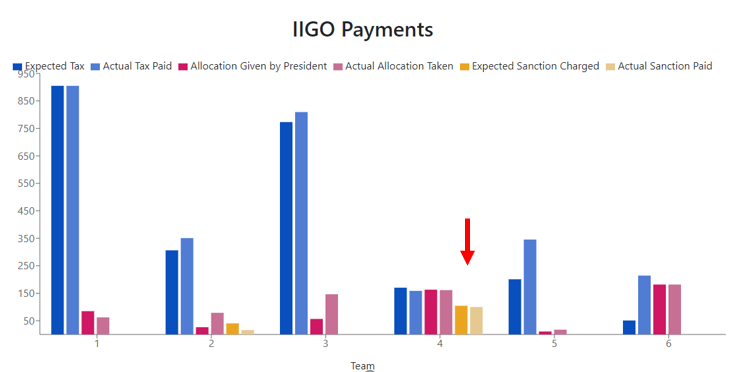
\includegraphics[scale=0.6]{12_team4_agentdesign/images/IIGOHO.PNG}
\caption{IIGO Payments For Honest Client Versus Other Teams.}
\label{fig:IIGOHO}
\end{figure}

\begin{figure}[H]
\centering
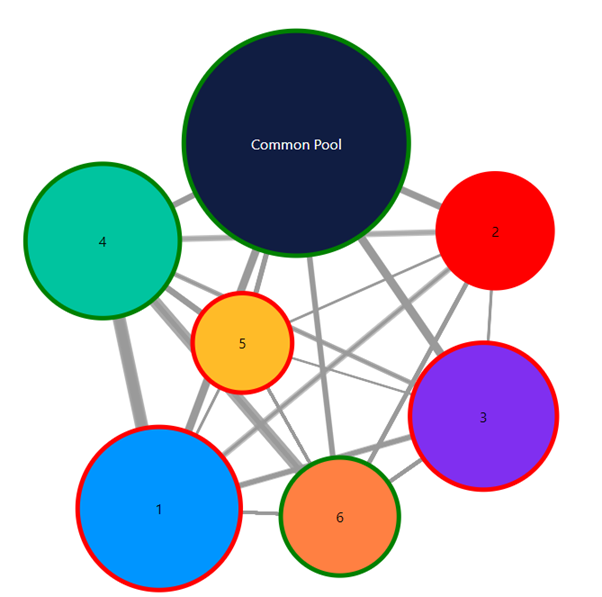
\includegraphics[scale=0.4]{12_team4_agentdesign/images/TransactionsHO.png}
\caption{Transactions For Honest Client Versus Other Teams.}
\label{fig:TransactionsHO}
\end{figure}
\begin{figure}[H]
\centering
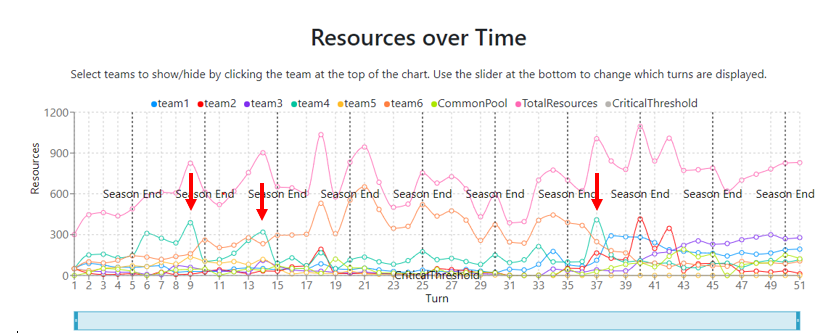
\includegraphics[scale=0.7]{12_team4_agentdesign/images/ResourcesHO.PNG}
\caption{Resources Plot For Honest Client Versus Other Teams.}
\label{fig:ResourcesHO}
\end{figure}

\subsubsection{Moderate Client} \label{moderateAO}
The \emph{moderate} client is configured specifically to start the game with an internal set of parameters that would allow it to score values as close as possible to thresholds in each decision making matrix calculation. The team opted for such a design choice in order to maximise the agent's response time to the environment, making it much more flexible than its two counterparts, who take a longer time to modify their strategy. As a Moderate client was simulated against other teams, the team noticed that it would perform very similarly as the Honest agent, as the other teams were always run on a "honest-like" configuration. Similarly, it would quickly turn its behaviour to dishonest when running against dishonest-like implementations of other teams' agents.

\subsubsection{Dishonest Client}
The \emph{dishonest} client, aptly named, is designed to take advantage of a large amount of common resources without collaborating with others and systematically abusing positions of power to gain economical advantages. The yielded results highlighted an interesting behaviour of the system and of other agents. As per design, the system is not flexible enough to mitigate such radical and rogue behaviour, resulting in a complete dominance of the dishonest agent. The agent proceeds to appropriate of all resources from the common pool and mercilessly watch other islands die, as profiled in Figure \ref{fig:ResourcesDO}. Eventually unable to survive without the collective help to mitigate disasters, it slowly meets its demise. The other agents do not reach a level of understanding of the game that allows them to comprehend what is going on and try to mitigate it by enforcing more severe rules. It must also be said that the system itself does not allow any hard enforcement, making it impossible for other agents to counter-attack a fully dishonest and selfish strategy, which disregards sanctions and taxes. Given these findings, dishonesty might seem like a dominant strategy as the agent survives the longest, securing all resources for itself. However, the long term dilemma imposes that islands must collaborate to survive for long periods. The dominance of this strategy is fatherly refuted by the simulations performed in subsection \ref{dishonestAD}.

\begin{figure}[H]
\centering
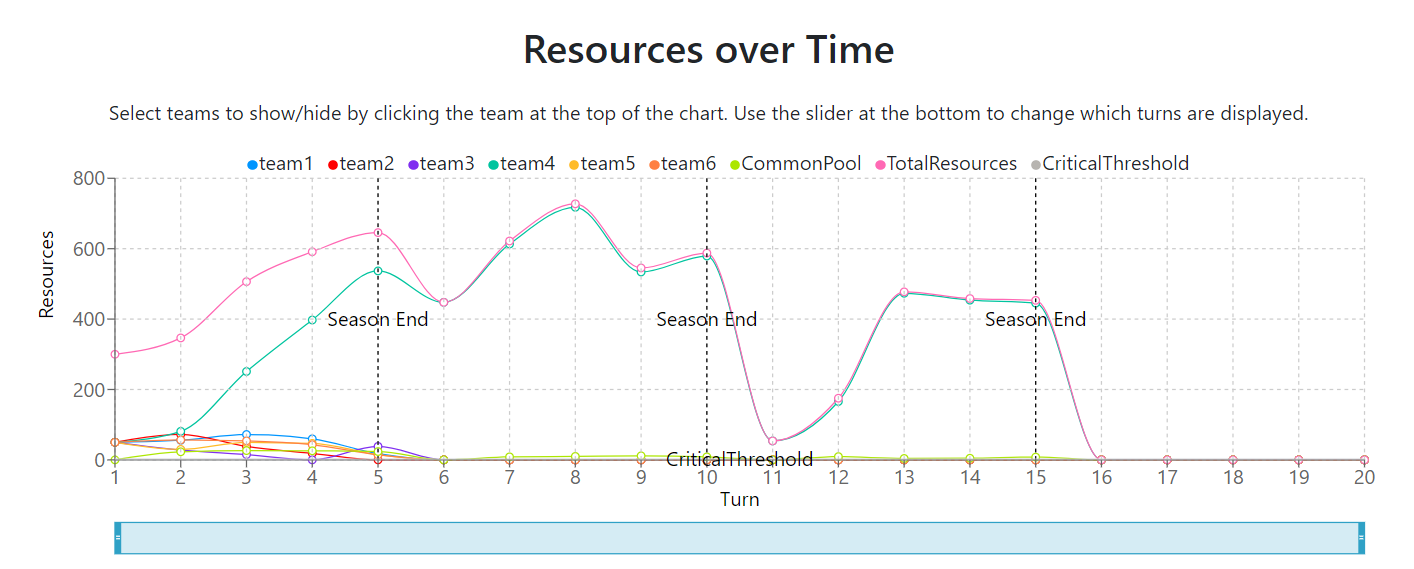
\includegraphics[scale=0.4]{12_team4_agentdesign/images/ResourcesDO.png}
\caption{Resources Plot For Dishonest Client Versus Other Teams.}
\label{fig:ResourcesDO}
\end{figure}

\subsection{Uni-Agent Simulations} \label{againstself}
Simulating our agent against instances of itself raised some interesting talking points. The main issue identified can be referred to as a \emph{lack of variety}, which encompasses the problem of populating the archipelago with islands that share the same "mindset"; therefore, approach dilemma from a unified prospective. This hypothesis was raised as an attempt to explain the poor results of uni-client simulations which have been observed not only when running team 4 agents against themselves, but also when other teams' agents were put against themselves under the uni-agent settings.

In all uni-agent simulations, the common pool was initialised to 10,000 resources, so that the agents could have enough resources to initialise running IIGO sessions.

\subsubsection{Honest Agents Only}
Populating the game with only honest clients provided a starting environment where all clients in the game are inclined to obey to rules and contribute a lot to the common pool in collective efforts. From this standpoint it makes sense that clients would build strong relations of trust and retain a high opinion of each other, as they treat each other with a fair and collaborative personality. Therefore in the evolution of the game, no agent undertakes any radical change of personality as was the case when our honest client was placed against other teams in subsection \ref{honestAO}. The IIGO Payments histogram in Figure \ref{fig:IIGOHH} nicely shows how the islands do not break any rule throughout the entire run.

It also manifests a very predictable behaviour of each honest agent that is perfectly in line with their design, such as paying more taxes than requested and taking less allocations than granted. The team identified this predictable behaviour as an example of \emph{lack of variety} that shows how agents with the same specification are not adaptive enough to survive in such a complex system that begs for a variety of strategies to be properly discovered and efficiently exploited.

\begin{figure}[H]
\centering
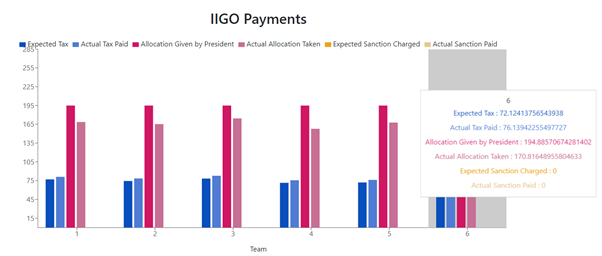
\includegraphics[scale=0.8]{12_team4_agentdesign/images/IIGOHH.png}
\caption{IIGO Payments For Honest Clients Only.}
\label{fig:IIGOHH}
\end{figure}

\subsubsection{Moderate Agents Only}
As presented in subsection \ref{moderateAO}, moderate agents are specifically designed to increase the variance in agent strategy. As a result, the \emph{lack of variety} issue should have been mitigated in a simulation where moderate agents face each other. After running the simulations, the clients have indeed acted far less predictably. Comparing Figure \ref{fig:IIGOMM} with the histogram plot shown in Figure \ref{fig:IIGOHH}, the breadth of a larger variety of game strategies can be observed. Namely, agent 2 and 3 show more dishonest traits, hence getting sanctions for performing illegal actions. Meanwhile, other clients take a more honest approach which replicates the ones observed by the honest clients. For other clients, like number 6, this honest strategy is less pronounced.

\begin{figure}[H]
\centering
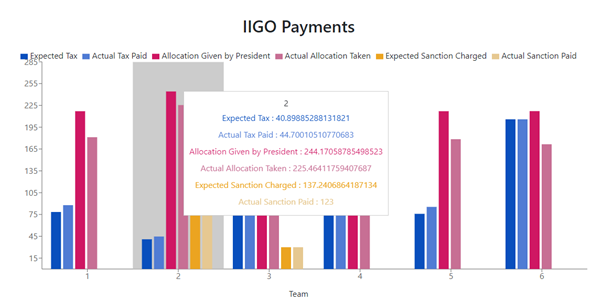
\includegraphics[scale=0.8]{12_team4_agentdesign/images/IIGOMM.png}
\caption{IIGO Payments For Moderate Clients Only.}
\label{fig:IIGOMM}
\end{figure}

Although the variance of agents strategy is significantly higher, clients still share the same underlying "mindset". This means that they define their whole personality using the same features, such as approaching tasks like foraging and power roles in the same way. Therefore, although the simulations ran show a slight improvement compared to "only honest" and "only dishonest" studies, they are far from producing a successful game like in multi-agent simulations. One of the main causes of this phenomenon was identified as the poor performance of actions that have been deliberately implemented in a simpler way in order to reduce the complexity of the agent. In particular, a foraging strategy in a well-performing multi-agent system may be to just replicate the foraging decision of the team that is economically strongest. However, in a uni-agent environment, this strategy  results in a group of agents mutually trusting their foraging strategy where nobody considers which one is actually the most profitable given the current circumstances.

Furthermore, features such as proposing rules is another good example of how lacking variety results in weaker archipelagos. This action enhances the ability of clients to adapt to the environment, crafting new rules as unexpected situations arise. If a client decides not to implement this feature in a multi-agent system, its effect on the adaptive capability of the archipelago will be almost fully mitigated by more complex clients that do perform such action. In a uni-agent simulation, such a feature wouldn't be present - severely crippling the survival chances of the islands.

\subsubsection{Dishonest Agents Only} \label{dishonestAD}
The last pure uni-agent simulation shows how dishonest clients face each other. This is, by far, the setting in which island longevity suffers the most as all clients start off the game with the intent to take advantage of the full resources with no compassion for others - demonstrating a textbook case of the tragedy of the commons. Runs in this environment feature one of the island who wins the race and empties the common pool, leaving other islands to die. The whole demise is made even faster by the total lack of collaboration among agents. Figure \ref{fig:ResourcesDD} demonstrates just how fast the archipelago is decimated. This comes as an additional proof of the fact that dishonesty cannot be considered a dominant strategy, indeed an honest or moderate client in such a setting would perform significantly better.
\begin{figure}[H]
\centering
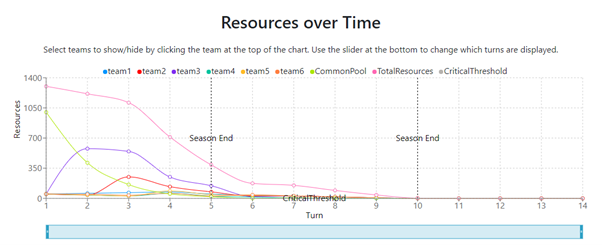
\includegraphics[scale=0.8]{12_team4_agentdesign/images/ResourcesDD.png}
\caption{Resources for Dishonest Clients Only.}
\label{fig:ResourcesDD}
\end{figure}

\subsubsection{Mixed Agents}
In an attempt to overcome the \emph{lack of variety} problem, simulations were run by instantiating two clients from each personality to promote variance. As demonstrated in Figure \ref{fig:IITOTransMA} via the “transactions” and “IITO” plots, the honest and moderate islands dominate in contributing to the community and share resources compared to the two dishonest clients “5 and 6”. Despite the clear difference in approaches from interaction plots, the game is still destined to finish early - failing to over come \emph{lack of variety}. This may be because agents are still sharing the same underlying “mindset” as they take decisions based on the same thresholds. They also are structured in the same way, so specific strategies like foraging or optional actions like proposing rules, if they are not implemented at all or just heavily relying on other clients making smart choices, will not work as well as in a more diverse environment.

\begin{figure}[H]
\centering
\begin{minipage}{.5\textwidth}
  \centering
  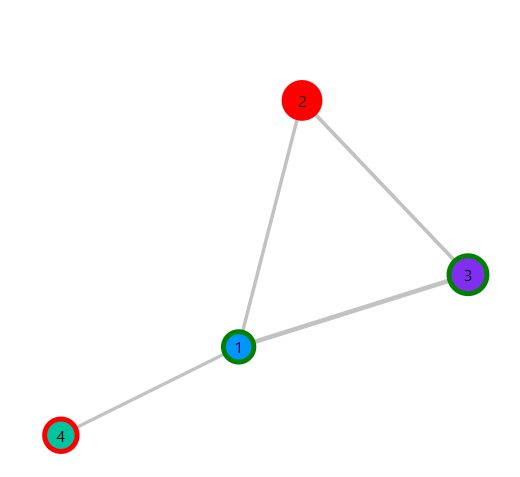
\includegraphics[width=.45\linewidth]{12_team4_agentdesign/images/IITOMA.png}
  IITO interactions
  %\captionof{IITO interactions}
\end{minipage}%
\begin{minipage}{.5\textwidth}
  \centering
  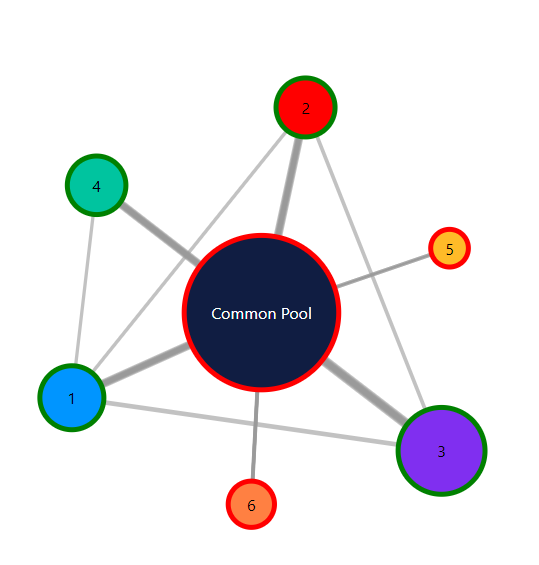
\includegraphics[width=.45\linewidth]{12_team4_agentdesign/images/TransactionsMA.png}
  Transactions
  %\captionof{Transactions}
\end{minipage}
  \label{fig:IITOTransMA}
  \caption{IITO interactions and transactions among mixed clients.}
\end{figure}


\subsection{Results Summary} \label{ResultSummary}
%Rudolfs suggestion on phrasing it as experts in the field allow all islands to thrive.%
\subsubsection{Lack of variety}
The \emph{lack of variety} problem was a reoccurring trend in all uni-agent systems. The question comes in when considering whether or not this trend was avoidable or not. Because the agents had a limited number of actions it could take, putting the same strategies up against each other resulted in a stalemate due to the lack of variance. By theory, this would be a problem regardless of what the specific implemented strategy actually contains.

This begs the question on whether an optimal strategy would even exist on a game such as this if all participating agents have the same level of complexity. A possible solution to this may include a type of state machine, an agent design our team has considered on the developing stages. The core concept is that an agent can implement different strategies depending on the situation the agent is put in. However, as demonstrated by the mixed agent uni-agent simulations, making a state machine with our three agents would not have been enough variance to overcome this issue. This indicates that in order to overcome the \emph{lack of variety} problem, it is not enough to have flexible thresholds and parameters - the agent's design approach itself must be radically different at each state. This would require a lot of rewritten and well-partitioned code which was not sufficiently formable in our limited time frame.

\subsubsection{Ostrom's Principles}
Evident by the behaviour of the dishonest agents, the tragedy of the commons was not overcome. To search for the cause of this, the system was compared with Ostrom’s principles.

A lot of Ostrom’s principles have already been enforced from the structure of the game in the form of the inter-island organisations:
\begin{enumerate}
    \item Clearly defined boundaries: The environment core infrastructure enforces the boundaries between agents.
    \item Congruence between rules and the local environment: IIGO sets different tax brackets per the agent status.
    \item Collective choice arrangements: Every agent can propose its own rules and vote existing rules off play.
    \item Monitoring by appointed agencies: The accountability cycle forms a monitoring system between the roles of power.
    \item Flexible scale of graduated sanctions: Sanctions are given in differing tiers accordingly to offences.
    \item Access to conflict resolution mechanisms: Not very applicable - discussion to be followed.
    \item Minimal recognition of right to self-organise: 
    \item System of systems: 
\end{enumerate}
In this client implementation, principle 3 is missing as the agents do not propose their own rules. Principle 6 is also missing, but this is less clear as to how this would be implemented. The way the game is made, there isn't a lot of room for conflicts to rise between islands, as the only interactions the agents have are in the form of gifts while the only form of opinions exist in the form of internal parameters which are not shared across agents.

This brings rise to the question as to whether Ostrom’s principles would be applicable to a non-ML based agent, and whether Ostrom’s rules require human behaviour as a prerequisite. Even if some rules were pre-made and given to the agents to propose and take down as the agents please, these rules wouldn't be an effect of the agents' organising - it would be an enforcement by us, the makers of the agents. One way to properly implement rule 3 would be to make the agent spontaneously create rules or create all possible rules based on its understanding of the situation of the game, which requres effective collection of all useful information from the game, as well as successful interpretation of the information. In addition, the agent would need to predict the how rules interact with each other, which is not trivial even for humans. Based on this, a further investigation of this could be done by measuring how much human influence can loom over the agents design, and its relevance to the applicability of Ostrom’s principles.

    \chapter{Team 5 Agent Design}
\section{Game Specification}
Our agent represents an island that exists in the Archipelago where it interacts and collaborates with other islands (agents). All agents interact with a Common Pool of resources which is primarily used to facilitate governmental procedures and mitigate natural disasters that may occur (long-term collective risk dilemma). As a result of the short-term collective risk dilemma, there is not enough resources to satisfy all of agents but only enough to satisfice \textit{some} of them. According to \textit{Self-Organizing Multi-Agent Systems} by Pitts, satisfy means having all agent's needs taken care of. On the other hand, satisfice means only the basic needs/minimum requirements have been met. In this economy of scarcity, it may be sufficient that the agent's needs are satisficed. Each island presumably will have the objective of maximising its individual utility which requires collaboration with other islands.

In our implementation, the levels of resources held by our agent are divided into 'wealth tiers' which influence our agent's decision making strategies. Our interactions with other agents are driven by our \texttt{opinion} of them which evolves over time in the game. In every round, our agent computes its current wealth status and updates its opinion of others based on various factors explored below.

\subsection{Wealth Tiers}
We have defined four different wealth tiers and the respective thresholds to represent the status of the agent according to its current resources. The wealth tiers are defined as follows:
\begin{enumerate}
    \item \texttt{dying}: critical status. 
    \item \texttt{imperialStudent}: lower class (<30\% of starting resources).
    \item \texttt{middleClass}: middle class (<95\% of starting resources).
    \item \texttt{jeffBezos}: upper class (<200\% of starting resources).
\end{enumerate}

\subsection{Opinion Formation}
\label{subsec: opinion-formation}
\subsubsection{Design}
An opinion of other islands is our agent's general perception of them and is characterised by a \textit{general score} and a \textit{forecasting reputation}. Both are characterised by a score ranging from $1$ to $-1$, where $1$ represents the best possible perception of another island, and $-1$, the worst perception. A score of $0$ represents a neutral or indifferent opinion. We believe it is necessary to form opinions on more than one basis as opinion-oriented decisions may depend on different factors across various tasks. For example, it may happen that one agent is particularly stingy with gifting but is a very skilled forecaster. If our agent was then to decide which agents' forecasting data to trust, it would not make sense to exclude these agents on the basis of their stinginess, even though this may affect our propensity to share gifts with them in another part of the simulation.

While opinion formation is explored more in detail below, some potential events that may affect our opinion of other teams are as follows:
\begin{itemize}
    \item Allocating or distributing less than they initially offer for gifting.
    \item Giving allocation of common pool's resources to islands when holding the President role. 
    \item Sharing foraging information.
\end{itemize}

\subsubsection{Agent Implementation}
A structure has been implemented to provide the ability to potentially incorporate further attributes that influence our agent's opinion of others (each such attribute is termed an \texttt{opnionBasis} in the implementation). Current opinions are stored and updated in an \texttt{opinionMap} that is indexed by the IDs of other agents. Finally, a history of opinions per agents across turns is stored in an \texttt{opinionHistory} variable. This allows us to analyse how opinions evolve across time. The choice to include an opinion of our own agent in the aforementioned \texttt{opinionMap} was so the opinion of our agent can be adjusted based on the same measures that are used to form opinions of other teams. This allows for an interesting analysis how our agent performs given its own `behaviour’(essentially what our opinion of it would have been if it was another agent). Furthermore an addition parameter called "mood" was implemented into the agents behavior, mood directly affects how much the opinions of agents change by. When the agent is in \texttt{imperialStudent} tier opinion changes are magnified as the agent is under stress from the need to survive. Whilst if the agent is in the \texttt{jeffBezos} tier it is much more care free and his opinion will not change as much with useful or useless information. 

\section{Environment}
\subsection{Foraging}
\subsubsection{Design}
Our agent initially determines its foraging method through its wealth tier during the initial foraging turns (three turns which can be adjusted in agent configuration). The agent will attempt deer hunting if it is wealthy (\texttt{jeffBezos} tier) as deer hunting is a high risk foraging method with larger potential returns. Since the agent already has a large sum of money, a negative return is less significant in comparison to if it was poor. The agent will contribute a randomly selected amount between $20\%$ and $30\%$ of its wealth (changeable in the configuration). Whilst in the \texttt{middleClass} and \texttt{imperialStudent} tier it will only contribute $10\%$ to $20\%$ of its wealth. Furthermore, in the \texttt{middleClass}, the agent has the equal chance of either deer hunting or fishing. In the \texttt{ImperialStudent} tier, the agent will choose fishing as it is poor and needs to avoid risk to survive. Finally when we are in the dying tier, at risk of dying in three turns, we invest all our money into fishing in hopes that we can catch at least a single fish and make it out of the dying tier. After every round the agent stores all its past experiences in its foraging history in addition to other agents past experiences if they were shared.  

Our agent executes the following steps to determine its foraging method:
\begin{itemize}
    \item First it enters \texttt{InitialForage()}) as described above.
    \item After the initial foraging it proceeds to do \texttt{normalForage()}) which is based off the foraging history stored from the initial turns. The agent first looks to find the best foraging method using (\texttt{bestHistoryForaging()}).
    \item \texttt{bestHistoryForaging()} First looks at the foraging history and calculates the average Return on Investment (RoI) its entire foraging history which is calculated using:
    \\  \begin{center} $\dfrac{output}{input}-1$ \end{center}
    \item In the case that the average RoI is less than 0 for both methods (no profit) then it returns none which indicates that there is no best foraging method. Otherwise it set the best foraging method as the one with the highest average RoI. 
    \item If the average RoI is above 0 then the agent assigns a probability of $10\%$ (set in configuration) to switch to either hunting or fishing.
    \item Afterwards, it looks at the number of hunters in the previous three turn (set in configuration). From this it will decrease the random probability of selecting deer hunting, the amount it decreases will depends on how close to the current turn the hunter went hunting. The closer to the current turn the lower the chances to hunt, additionally it also looks at the number of deer caught, if no deer were caught then the chances will not decrease. This can be seen in Table~\ref{table:Probability Avoiding Deer Hunting} . The number of deer caught would be halved and multiplied into the the probability.
           {\begin{table}[]
                 \begin{center}
                 \caption{Probability table of avoiding deer hunting according to the number of hunters in the past 3 turns (with scaled version (0.035))}
                 \label{table:Probability Avoiding Deer Hunting}
                        \begin{tabular}{|c|c|c|c|c|c|c|c|c|}
                        \hline
                                                 &   & \multicolumn{3}{c|}{Turns before current   hunt} &         & \multicolumn{3}{c|}{Turns before current   hunt scaled} \\ \hline
                                                 &   & 3                  & 2             & 1           & Scaling & 3                  & 2                & 1               \\ \hline
                        \multirow{6}{*}{Hunters} & 1 & 0.333333           & 0.5           & 1           & 0.035   & 0.011667           & 0.0175           & 0.035           \\ \cline{2-9} 
                                                 & 2 & 0.666667           & 1             & 2           & 0.035   & 0.023333           & 0.035            & 0.07            \\ \cline{2-9} 
                                                 & 3 & 1                  & 1.5           & 3           & 0.035   & 0.035              & 0.0525           & 0.105           \\ \cline{2-9} 
                                                 & 4 & 1.333333           & 2             & 4           & 0.035   & 0.046667           & 0.07             & 0.14            \\ \cline{2-9} 
                                                 & 5 & 1.666667           & 2.5           & 5           & 0.035   & 0.058333           & 0.0875           & 0.175           \\ \cline{2-9} 
                                                 & 6 & 2                  & 3             & 6           & 0.035   & 0.07               & 0.105            & 0.21            \\ \hline
                        \end{tabular}
                \end{center}
            \end{table} }  
    \item The probabilities to switch foraging methods are summed and applied to the method with the highest average RoI, resulting in the foraging method of choice
\end{itemize}

Now that our agent has decided its method of foraging, it needs to determine the amount of resources to contribute
\begin{enumerate}
    \item In the case the best foraging method is none where no RoI was positive:
        \begin{itemize}
            \item The agent will skip foraging for one turn.
            \item If the agent has already skipped last turn, then it is forced to forage as there is a need to get resources to survive. It will randomly select the foraging method and enter double the amount of resources it would normally invest (10\% to $20\%$) with, in hopes it could catch at least a single fish or deer.
        \end{itemize}

    \item In the case a method has positive RoI:
        \begin{itemize}
            \item It look at the input that gave the best RoI for that foraging method in addition to the method that gave the best profit.
            \item Then it takes a percentage of both best RoI and best profit, and added a random amount from ±$5\%$ of its total resources as its contribution.
            \item Looking at the number of islands alive, it then increases its contribution the less islands that are alive. This is to avoid contributing insufficient resources when other islands die and we are unable to reach the threshold to catch any animals. 
            \item Finally it restricts our contribution to a maximum of $40\%$ of our wealth.
        \end{itemize}
\end{enumerate}

Our agent's general opinion of others is heavily affected by the information available from other agents, thus if other agents refuses to share their foraging data, our agent will also stop sharing foraging data and have a lower opinion of them as well. \newline


\textbf{Future Works}\newline 
In future implementation, it would be interesting to investigate the application of machine learning techniques for the following tasks:
\begin{itemize}
    \item Determining the optimal foraging method or location if multiple foraging zones are implemented.
    \item Determining the best way to communicate with other agents in a way that may influence their foraging behaviours to benefit our agent.
\end{itemize}

\section{Inter-island Governmental Organisation (IIGO)}
\subsection{Common Pool}

The agents can request resources from the common pool, get their allocation and contribute to the common pool. The overall intention of each agent is to maximize utility and thus, our agent tries to estimate each legitimate claim in every round and ask for the highest possible allocation amount that would be accepted by the President. Additionally, there are some specific scenarios that our agent seeks for more resources than it "deserves" because it is low in resources. In these critical scenarios, the agent not only asks for more but also tries to steal from the common pool and does not contributes to it, to assure its survival. Thus, the strategy of our agent is shaped as follows: \newline

The agents requests for the permission from the President to take resources from the common pool and the President replies with the allocation amount. The requested amount depends on the \textit{turn}, the \textit{wealth status} of our agent and the \textit{allocationHistory} from the President. if \textit{allocationHistory} indicates approval of allocation amount of the President in the latest turn, the agent will request a higher amount of resource compare to the said allocation amount in \textit{allocationHistory}. However, if the President refused to allocate any resource to the agent lately, the agent will request a minimum amount to survive, which is $30\%$ of the initial resources given to an island, when it needs help from the common pool.


Every turn, our agent will decide if it can or needs to take any resource from the common pool. Ideally, the amount of resources taken from the common pool should be equal to the allocation amount given by the President. However, that is only true when our agent is doing well regarding financial status, \texttt{middleClass} or above. When the agent is in poor financial state, it will try to take the minimum amount necessary to survive, even if it exceeds the amount approved by the President. \newline

The agents are asked to contribute an amount of resources for tax. In the ideal circumstances, our agent will contribute at least the minimum amount of tax to the common pool to help funding IIGO operations. However, when our agent is in a poor state, below \texttt{middleClass}, it will ignore tax until it can get back on its feet once again. \newline

Our agent also contributes to the common pool to help the community. The important factor that decides if our agent will contribute or not is the flow of resource in the common pool since the last turn. If the flow is negative, it indicates that the trend of roles and other agents is to spend more than to contribute to the common pool. In that case, our agent will not make any contribution to the common pool. However, if the contribution is higher than the spending, our agent will contribute $1/6$ of the positive flow of resources to the common pool to assist the community. Unfortunately, if our agent in a poor financial state, it will ignore this contribution until it can get back to the normal state. \newline

Beside contributing to help the community, our agent also tries to use the common pool for disaster mitigation. This contribution is determined based on our disaster forecast's \textit{magnitude}, \textit{epicentre}, \textit{period}, \textit{confidence interval},  and the agent's current \textit{wealth}. From these values, an ideal contribution amount will be calculated. The confidence interval indicates the ideal amount of resource to contribute to the common pool. It is done this way to ensure our agent does not waste a lot of resources in case of uncertain predictions. In cases where predictions were made with higher certainty, the agent will want to ensure that the damage is mitigated when the incident happens. The ideal contribution is proportional to the damage and inversely proportional to the distance between the island and disaster's epicentre. Our agent will only contribute $20$\% of the ideal contribution $1$ day before the disaster may hit. The other $80$\% will be given on the day of the predicted disaster. This is to ensure that the purpose of the contribution (mitigating disaster) will be preserved. And since disaster occurs after IIGO events, it is acceptable to donate most of the resources on the day of the disaster. In cases where our agent's resources is not sufficient to match the calculated amount above, it will contribute $50$\% of its current resources for the purpose of mitigating the disaster. \newline

\subsection{Opinion Formation in Common Pool Transactions}
Our agent looks at how the the allocation has been given by the President and updates its opinion score with respect to the agent acting as the President. This helps form positive perception to President who tries to support fellow agents whenever having the mean to. The opinion score changes as follow:



\begin{itemize}
    \item If there is no allocation from the President even when there's sufficient amount in the common pool, it will cause a negative effect to opinion score.
    \item If the allocation is less than what was requested, there will be a light negative effect to opinion score.
    \item If the President approves an allocation amount equal to greater than the requested amount, there will be a positive effect to opinion score. 
\end{itemize}

\subsection{Sanction Payments}
Sanction are imposed when an agent breaks the rules such as stealing from the common pool. Since ignoring sanction payment will lead to longer sanction period, our agent will always pay the entire sanction amount as long as it has enough of resources. 

\subsection{Monitoring Roles} 
Our agent decides whether or not to monitor roles based on its opinion towards the client holding office. It is done this way because monitoring requires resources from the common pool and unnecessary monitoring will take the resources away from those who need it most. Furthermore, our agent's opinion is formed based on how interactive and supporting the other agents are towards fellow agents, thus it is a reasonable metric to use.

\subsection{Future Work}
Currently, the salary and actual spending of IIGO roles are not public to the agents. It would be a huge improvement to analyse the flow of resources in the common pool. The decision to contribute to the community through common pool will be more fair if those values are published. \newline

At the moment, the amount of contribution for mitigating disaster purpose is calculated based on only our agent's forecast. the model will improve a lot if the function takes into account predictions shared from other teams also. However, the agent may put a heavier weight on its prediction to make sure its not being tricked into contributing to the common pool for other purposes. 


\section{Inter-island Trade Organisation (IITO)}
\subsection{Gifts}
\subsubsection{Design}
Due to the short-term collective risk dilemma that is foraging, it is in the best interest of all the agents to keep other agents alive. Thus, not only does our agent requests for gifts but also offers gifts to others depending on its \textit{wealth tier}, the \textit{balance of resources} over the last turn and its \textit{opinion} towards the other agent. To form a well-rounded opinion and decide on the optimal strategy, our agent keeps track of the gift history and continuously updates its general opinion towards the others once it receives gifts. \newline

In the case that our agent is in \texttt{jeffBezos} or \texttt{middleClass} wealth tiers, it will assist other agents. The amount our island can give is limited to a percentage of its total resources which scales according to the wealth tier, the higher the wealth tier the greater the percentage as the agent has an abundance of resources. If our agent is in \texttt{imperialStudent} tier, it can partially assist agents that are in critical condition, however it will look to keep its resources for survival. Thus, it will not give any gifts to agents that are not in critical condition or have a low opinion of. Whilst, if our agent is in \texttt{Dying} status it can barely survive so it does not have the luxury to offer other agents resources. For the same reason, it does not request from islands that are in \texttt{Critical} status.  \newline

Our agent stores all of its gifting history to modify its opinion on other agents and act based on this. In more detail, when our agent has a positive opinion towards another agent it attempts to maximise their satisfaction and offers them an amount equal to what they requested for, depending on the wealth tier our agent is in . The higher the wealth tier the close our agent offers what was requested. In contrast, if they have a negative opinion it takes less consideration of their requests and more of what our agent wants to offer. All of the requests are limited to a certain percentage of our resources which is dependant on our wealth tier. \newline

Overall supporting other agents is beneficial in the long run, as the more agents that survive the more likely they can mitigate greater risk of the long-term Collective Risk Dilemma. By offering to the others, when our agent has the capacity to do so, our agent attempts to make them have positive views towards it. This is advantageous as other agents are likely to assist our agent when in need, with either gifts or assistance when they occupy one of the three government roles. Furthermore, when our agent is in lower wealth tiers it reduces the offers to other agents and focus on its own survival regardless of others opinions on our agent.

\subsubsection{Role of opinions in gifting}
More specifically, our agent stores previous gift history in \texttt{giftHistory} the gift history holds:
\begin{enumerate}
    \item What it requested; What was offered to it; The amount it accepted with the reason and The actual received amount.
    \item What they requested for; What our agent offered them; The amount they accepted with the reason and What they actually received.
\end{enumerate}

In each turn, our agent adjusts its opinion towards the others using a method called \texttt{giftOpinions}:
\begin{itemize}
    \item Negative Effect: Received less than offered.  
    \item Slight Negative Effect: Offered less than requested.
    \item Slight Negative Effect: If they requested the most compared to the others.
    \item Slight Positive Effect: Received more than they offered.
    \item Slight Negative Effect: If they requested the least compared to the others.
    \item Positive Effect: Received more than requested.
\end{itemize}

To calculate the request amount our agent uses a function called \texttt{GetGiftRequests} which requests gifts, in the the \texttt{jeffBezos} Tier,  from all other agents that are not in Critical state to maximise our utility. Depending on our wealth tier and opinion of other agents the amount requested will vary, requesting less from agents with higher opinion scores. To calculate the amount our agent offers, there is a function called \texttt{GetGiftOffers} which takes into consideration the requested amount from each team and returns a counter offer according to their opinion level and our wealth tier. The function \texttt{GetGiftResponses} obtains the response offer that we get from other teams and accepts all the offers that were give to our agent as there is no reason to decline gifts that could benefit our agent no matter the amount. \newline

{\textbf{Future Works}}\newline
Currently, the higher the opinion we have the less we request from an island. However, the a unique dynamic could be implemented where if the agent can meaning that we would be exploiting the positive relationship with our highly rated islands, asking for more. Furthermore, we could have looked into the amount of resources that islands were giving us in total to further adjust how we grade our opinion of them. 

\section{Inter-island Forecast Organisation (IIFO)}

IIFO implementation covers making disaster predictions/forecasts based on a history of disaster observations and predictions from other teams. 

\subsection{Basis of Forecasts}
The forecasting implementation generates forecasts based on several factors as explored below.

\subsubsection{Experience}
Most importantly, we use our past observations of disasters that occurred in \texttt{disasterHistory} to inform our current and future forecasts. Forecasts attempt to predict the following characteristics of a disaster:
\begin{enumerate}
    \item\textbf{(x,y) co-ordinates} of disaster epicentre.
    \item \textbf{magnitude} (severity) of disaster.
    \item \textbf{period} - the time (number of turns) between successive disasters. For a given forecast, this will involve predicting the time until the next disaster.
\end{enumerate}

One effective way to capture this notion of experience is to estimate the probability distribution function (pdf) of the underlying process that generates these disasters. However, given that agents are not provided any knowledge of these distribution functions, they can only make estimates using sample data collected through their interaction with the environment. Given that agents have no \textit{a priori} knowledge about distribution types, parametric estimation methods such as MLE (maximum likelihood estimation) are not suitable. Instead, kernel density estimation (KDE) was employed to estimate the pdf of each forecast variable (as listed above). KDE is a non-parametric approach to estimating a pdf and does not require any knowledge about the type of distribution. For a univariate iid sample $x_1, x_2, \dots, x_n$ and unknown pdf $f$, the KDE estimate $\widehat{f}$ is given by Equation~\ref{eq: KDE Estimate}.

\begin{equation}
\widehat{f}_{\gamma}(x)=\frac{1}{n} \sum_{i=1}^{n} K_{\gamma}\left(x-x_{i}\right)=\frac{1}{n \gamma} \sum_{i=1}^{n} K\left(\frac{x-x_{i}}{\gamma}\right)
\label{eq: KDE Estimate}
\end{equation}

where $K$ is the non-negative kernel function with bandwidth $\gamma$. While many different kernels may be used, a Gaussian kernel was exclusively used in this implementation. The bandwidth represents the width of each Gaussian "hump". Larger bandwidths result in a larger degree of smoothing. The literature details a few mechanisms for selecting an appropriate bandwidth based on data, and in this implementation, the Scott rule-of-thumb method was used. The details thereof are not included for the sake of brevity.

The KDE estimates for a normal distribution for varying numbers of samples using our implementation is shown in Figure~\ref{fig:KDE_uniform} below. Naturally, the estimated pdf more closely resembles the underlying counterpart with an increasing number of samples.

\begin{figure}[!htb]
    \centering
    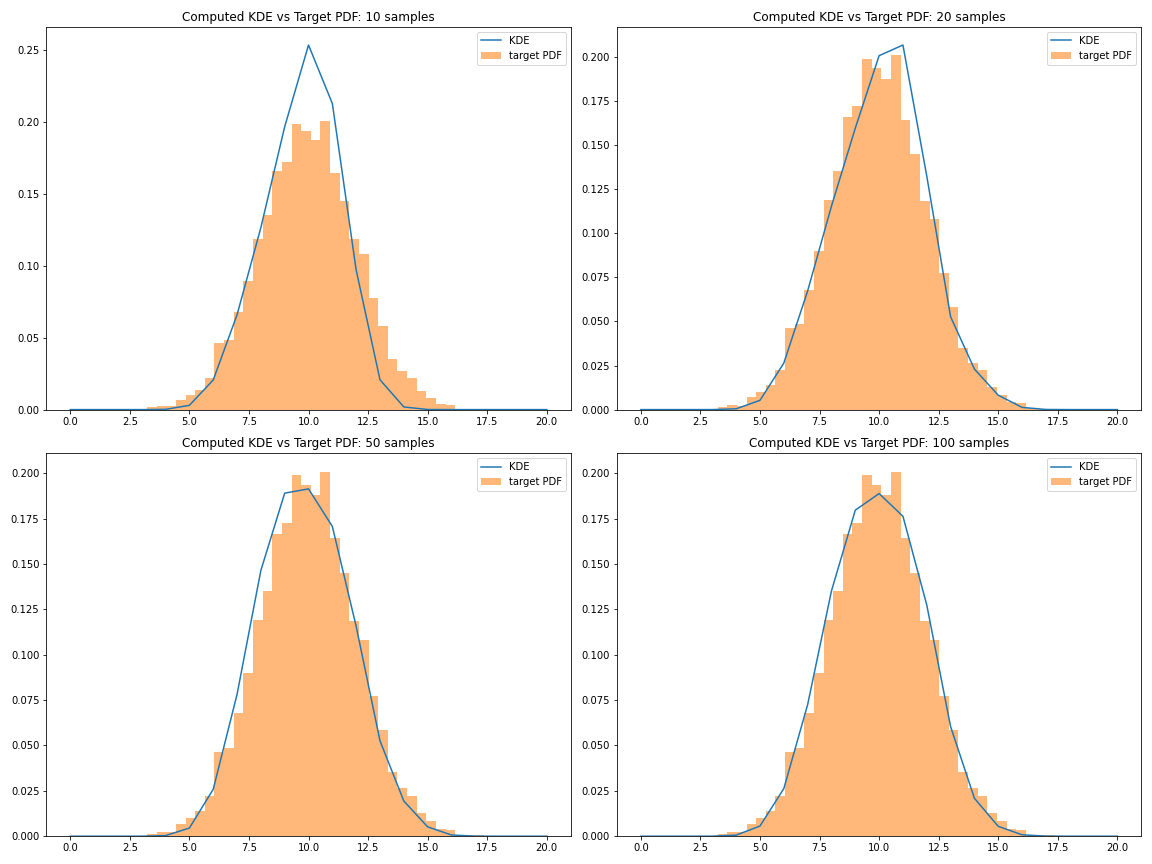
\includegraphics[width=0.82\textwidth]{13_team5_agentdesign/images/kde_plots.png}
    \caption{KDE simulation for a normal distribution for varying numbers of samples.}
    \label{fig:KDE_uniform}
\end{figure}

Another example of the efficacy of our KDE implementation is presented in Figure~\ref{fig:kde-exp}. Here, the distribution of disaster magnitudes - an exponential pdf - is estimated. The estimated PDF is remarkably close to the target, even with as few as 20 samples.

\begin{figure}[!htb]
    \centering
    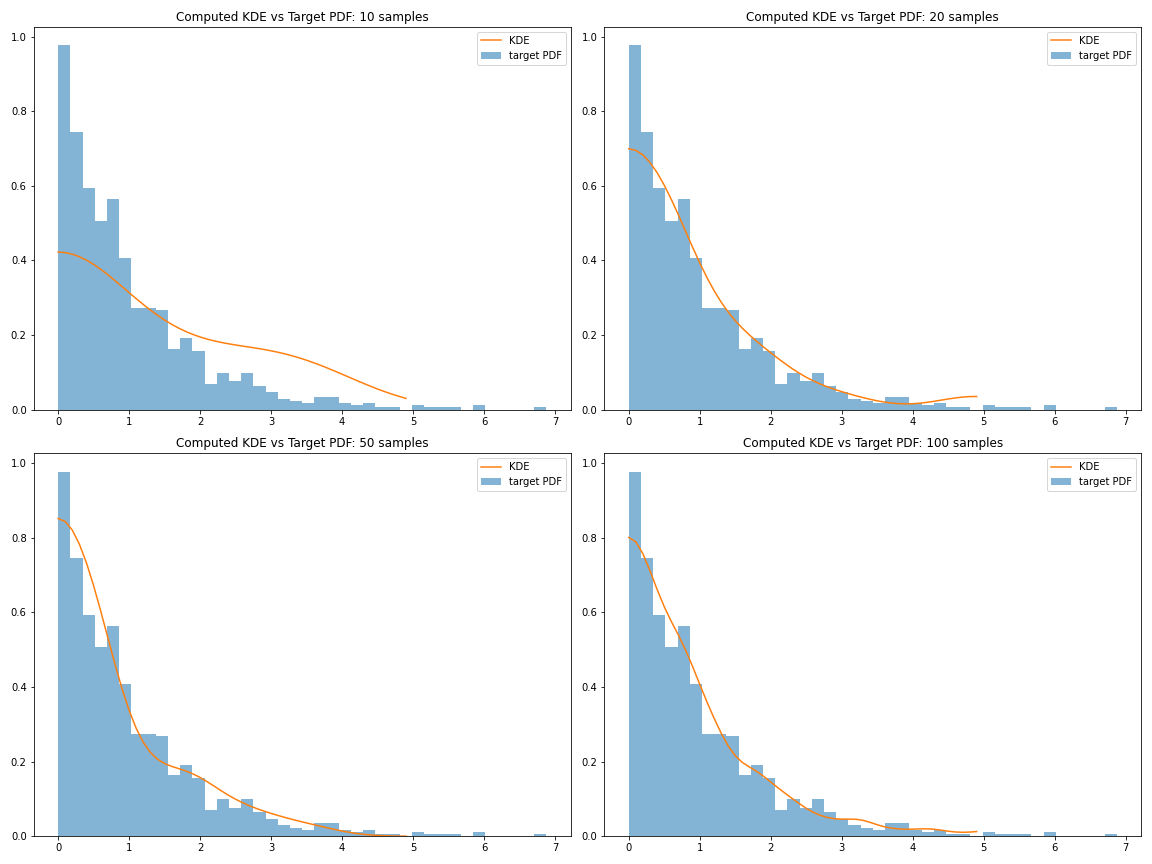
\includegraphics[width=0.82\textwidth]{13_team5_agentdesign/images/kde_plots_exp_deer_sizes.png}
    \caption{KDE of disaster magnitudes based on observed data against the true underlying exponential pdf for varying number of observed samples.}
    \label{fig:kde-exp}
\end{figure}

In our implementation, KDE was used to estimate the underlying distributions for each forecast variable of interest. These estimates evolve (become more accurate) with more data and so, our agent theoretically should become a more skilled forecaster with time.

\subsubsection{Confidence of forecasts}
Another important component of our agent's forecasts is its confidence. This is not only helpful in other decision making processes in our strategy (such as deciding how many resources to contribute to the Common Pool), but is also integral to our reputation amongst other agents. Clearly, if we're producing  inaccurate predictions with high confidence, other agents will quickly learn to no longer trust our forecasts and may begin to stop sharing their forecasting decisions. Therefore, confidence is used carefully and honestly in our implementation; with limited data or inadequate historical accuracy in our estimates, our prediction confidence will be low. As we receive more data and are able to verify the stability of our estimates, the associated prediction confidence increases gradually. 

Confidence for our agent's forecasts is computed based on the variance of observed data. Specifically, confidence $\kappa$ for a given variable $x$ is computed as follows in Equation~\ref{eq: Forecast Confidence}:

\begin{equation}
\kappa = \frac{\sigma_x}{\Delta_x} \quad \text{where} \quad \Delta_x = P_x^{(0.95)}-P_x^{(0.05)}
\label{eq: Forecast Confidence}
\end{equation}

In this definition, confidence is an effectively a notion of relative dispersion of the observed data. It is the ratio of the standard deviation of a variable $x$ and its range $\Delta_x$. Instead of the ordinary definition of range, $\Delta_x = P_x^{(0.95)}-P_x^{(0.05)}$ was used where $ P_x^{(n)}$ represents the $n^{\text{th}}$ percentile of $x$. This was decided to avoid the possibility of outliers obscuring $\kappa$. Evidently, if observed samples are densely packed around the mean value, $\sigma_x$ will be closer to $\Delta_x$ and confidence will be higher. The opposite is true for more dispersed observations.

\subsection{Collaboration}
The other important component of forecasting is incorporating forecasts from other teams. In each turn, we receive forecasts offered to us from other teams - a (possibly empty) subset of all teams. These collaborative forecasts are stored each turn. After each disaster occurs, our agent evaluates the \textit{forecast performance} of both itself and the other agents in the following manner:
\begin{enumerate}
    \item Analyse every forecast preceding the disaster and for each variable (magnitude, period etc), compute the squared error between the forecasted and actual values. 
    \item Compute the exponentially-weighted average of these errors for each variable. An exponential decay is chosen so as to weight more recent forecasts more. 
\end{enumerate}

Once these historically-aggregated forecasting errors are computed for all agents (including ours), we evaluate the forecasting skill of other agents relative to ours. For each agent (excluding our agent) and each forecast variable, compare the other agent's forecast error to ours in the following way in Equation~\ref{eq:Evaluate Forcasting Skills}:

\begin{equation}
\text{relative skill} = s := 1-\frac{\epsilon_i}{\epsilon_*},\quad i \in \mathcal{A}_i, \quad |s| \leq 1
\label{eq:Evaluate Forcasting Skills}
\end{equation}

where $\epsilon_i$ is the forecast error of of agent $i$ for a given variable, $\epsilon_*$ is our agent's error for this variable and $\mathcal{A}_i$ is the index set of all agents. This skill value $s$ can be interpreted as follows:

\begin{itemize}
    \item $s < 0$: other agent is less skillful than ours at forecasting a certain variable
    \item $s = 0$: other agent's skill is on par with that of our agent
    \item $s > 0$: other agent is more skillful than ours at forecasting a certain variable 
\end{itemize}

These skill values are directly used to update our perceived forecasting reputation (part of opinion) of other islands.

Our evaluation of the confidence of other agents' forecasts is performed in exactly the same manner as ours. Forecasts with unrealistic confidence values - either in the absolute sense or relative to the amount of data available - will be held in lower regard. The forecasting reputation (explored below) of the agents responsible for such forecasts would be adjusted accordingly. 

\subsubsection{Role of opinions in forecasting}
As described in Section~\ref{subsec: opinion-formation}, our agent's opinion formation is an important mechanism for choosing which agents to exchange forecasting information with. Specifically, the \texttt{forecastingReputation} variable stored in our agent's \texttt{opinionMap} represents its evaluation of the forecasting skill of each other agent based on historical data. Some examples of how the \texttt{forecastingReputation} of other agents is updated by our agent:
\begin{itemize}
    \item An agent's reputation value is decreased if they make a nonsensical prediction with over $50\%$ confidence before any disasters have occurred.
    \item Unfounded certainty is also punished: reputations are decreased if an agent makes a prediction with over $99\%$ confidence and our agent detects that predicted variables are stochastic.
    \item Reputations are updated after each disaster based on calculated \texttt{forecastingSkill} which, as described above, quantifies another agent's average forecasting accuracy relative to ours. 
\end{itemize}

These reputation scores allow our agent to decide which agents' forecasting information to trust. Similarly, opinions allow our agent to choose which agents to share our \textit{precious} forecasting information with - if we simply share it indiscriminately, other agents may be less compelled to share their data as they would not lose in anything in not doing so. 

\section{Roles}
\subsection{President}
When our agent gets voted to be the the President, the following steps elaborate the strategy the President is going to take for each action point.
The President's role is to evaluate and allocate the common pool request resources. In order to evaluate a common pool request, the President assesses the size of the request and the current size of the common pool.The resource allocation has been divided into three possible scenarios: 
    \begin{itemize}
        \item If the request total is smaller than $80\%$ of the size of the common pool, then the President allocates all the requests.
        \item If the request total is between $80\%$ and the common pools current value, then the President divides the requests by two and then allocates them.
        \item If the request total is higher than the common pool size, then the President returns a fraction of those resources to the islands, keeping the common pool dynamics in order.
    \end{itemize}

Another commitment of the President is to set taxation amount to individual islands. Tax is necessary for IIGO roles and procedures to work. The President aims to set a fair tax amount to individuals proportional to their wealth. However, if an island chooses not report their wealth, a flat tax rate will be applied, which is high enough to encourage agents to be transparent about their resources. 

Furthermore, the islands will propose different sets of rules to alter the game specification, and the President selects one of the proposed rules to vote on.    
The President must also pay the Speaker its salary, for the Speaker to complete its tasks. In addition, the speakers salary is proportional to our agent's wealth. 
    \begin{itemize}
        \item When our agent is in \texttt{jeffBezos} tier, then, the Speaker salary is payed in full.
        \item When our agent has \texttt{middleClass} wealth tier, then only $80\%$ of the speakers salary is payed.
        \item When our agent is poor, which mean it is in \texttt{imperialStudent} wealth state, then only half of the speakers salary is paid.
    \end{itemize}

This strategy of paying the Speaker emphasizes the importance of preserving the Common Pool to the islands in difficult times. Since the agent has no way to look at others' wealth, it makes a rough estimation based on its own wealth. And since the common pool allocation strategy has no bias to any particular agent, the common pool is preserved for the well-being of agent in the difficult time. 

The President also has the task to decide the next Speaker. The President can manipulated the Speaker election and assigns the next Speaker based on our opinion of each team. The reason this strategy was implemented is because the agent's opinion is formed mostly based how much other agents try to help fellow agents. And it is an important characteristic that an important role should have.    

Moreover, the President sets the tax amount every turn, the tax rate is designed to be proportional to the islands resources in order to provide fair division of resources. However, if an island does not report their resources, then a strict tax rate is applied, which will essentially influence the islands to share the value of their resources with other islands. Additionally, the President is responsible to monitor the Judge's behaviour and hold the Speaker's election. 

\subsection{Speaker and Judge}
When our agent gets voted to become the Speaker or Judge, the following steps elaborate the strategy the agent is going to take for each action point.
The Judge has the privilege to pardon other islands. The Judge pardons agents who are highly regarded based on opinion scores. Similar to President's strategy, the agent pays the other role in the following way  to ensure the common pool's main focus is agents in difficult times. 

    \begin{itemize}
        \item When our agent is in \texttt{jeffBezos} tier, then the other role's salary is paid in full.
        \item When our agent has \texttt{middleClass} wealth tier, then only $80\%$ of salary is paid.
        \item When our agent is poor, which mean it is in \texttt{imperialStudent} wealth state, then only $50\%$ of the salary is paid.
    \end{itemize}
    
Furthermore, the Speaker and Judge hold elections for the other roles, a real winner will be voted on by the islands, but then our agent will announce the next Judge based on our opinions for aforementioned reasons.
    \begin{itemize}
        \item If our agent has bad opinion towards the real winner, which means opinion score is inferior to $0$, then our agent will choose another agent with highest opinion score to become the next Judge.
        \item if the real winner is on our agent's good side (a friend, score $> 0$), then he will be announced as the new role.
    \end{itemize}

\subsection{Voting for IIGO Roles}
Voting for IIGO roles are done based on our agent's current opinion on other agents. Our agent will always put itself on top of the vote and fill in other contestant from the candidate list based on opinion score from highest to lowest. This is a fair strategy to determine the IIGO roles since the agent's opinion is influenced by the interaction and devotion of other agents to the community. 

\subsection{Future work}
Currently, the agent only have one persona when acting as an official role. The personality of the role could be driven by its current wealth. Say if the agent is in \texttt{imperialStudent} state, it may try to find as much resources as possible, no matter how corrupted the process may be. The different personalities will add more dynamic to the simulation and it would be interesting to see how the agent would thrive or decline with different scenarios. 
\section{Simulation}

This section details the dynamics observed during the simulation of our agent's behaviour the other islands in the Archipelago. Once all agent implementations were finalised, simulations were performed using \textit{baseline} parameters. There is an extensive list of parameters that can be changed with no sensible initial values for many parameters, thus these baseline values had to be determined empirically. The environment is built on a variety of probabilistic models that introduce a lot of variance to the simulations. With this in mind, multiple simulations were run to allow us to evaluate our agent's behaviour in a broader sense.

By adjusting a single environmental parameter whilst fixing the rest we could capture the effect of a single parameter on our agent as well as the other agents. All tests were run twice so that extreme scenarios could be mitigated to some extent. If two consecutive tests returned similar results, these could be included in the overview\footnote{behaviours or results with sufficiently low variance to characterise with a general value or outcome} results.


\subsubsection{Foraging}

The objective was to observe the effect of altering foraging parameters on our agent's behaviour. Performance is quantified by the foraging efficiency of our agent, which is the ratio of output utility to resources invested. The selected parameters were varied around the baseline values and were then compared to baseline performance\footnote{performance using the relevant metric but with baseline parameters}

We first focus on deer hunting, using  \texttt{input proportional} and \texttt{equally distributed} return of the resources. The results are displayed in Table~\ref{fig:Foraging Deer Hunting Parameter Simulation Results}.

\begin{figure} [!htb]
    \centering
    
\includegraphics[width=1\textwidth]{13_team5_agentdesign/images/Foarging Simulation Deer Hunting.png}
    \caption{Foraging Deer Hunting Parameter Simulation Results}
    \label{fig:Foraging Deer Hunting Parameter Simulation Results}
\end{figure}

Next we changed the deer \texttt{OutputScaler} parameter. Once increased, we notice Figure~\ref{fig:Agent Resources Inversely correlated with the common Pool} shows that our agent is inversely correlated to the common pool resources. Therefore, the common pool resources decrease while our agent's resources increase, and vice versa.

\begin{figure}[!htb]
    \centering
    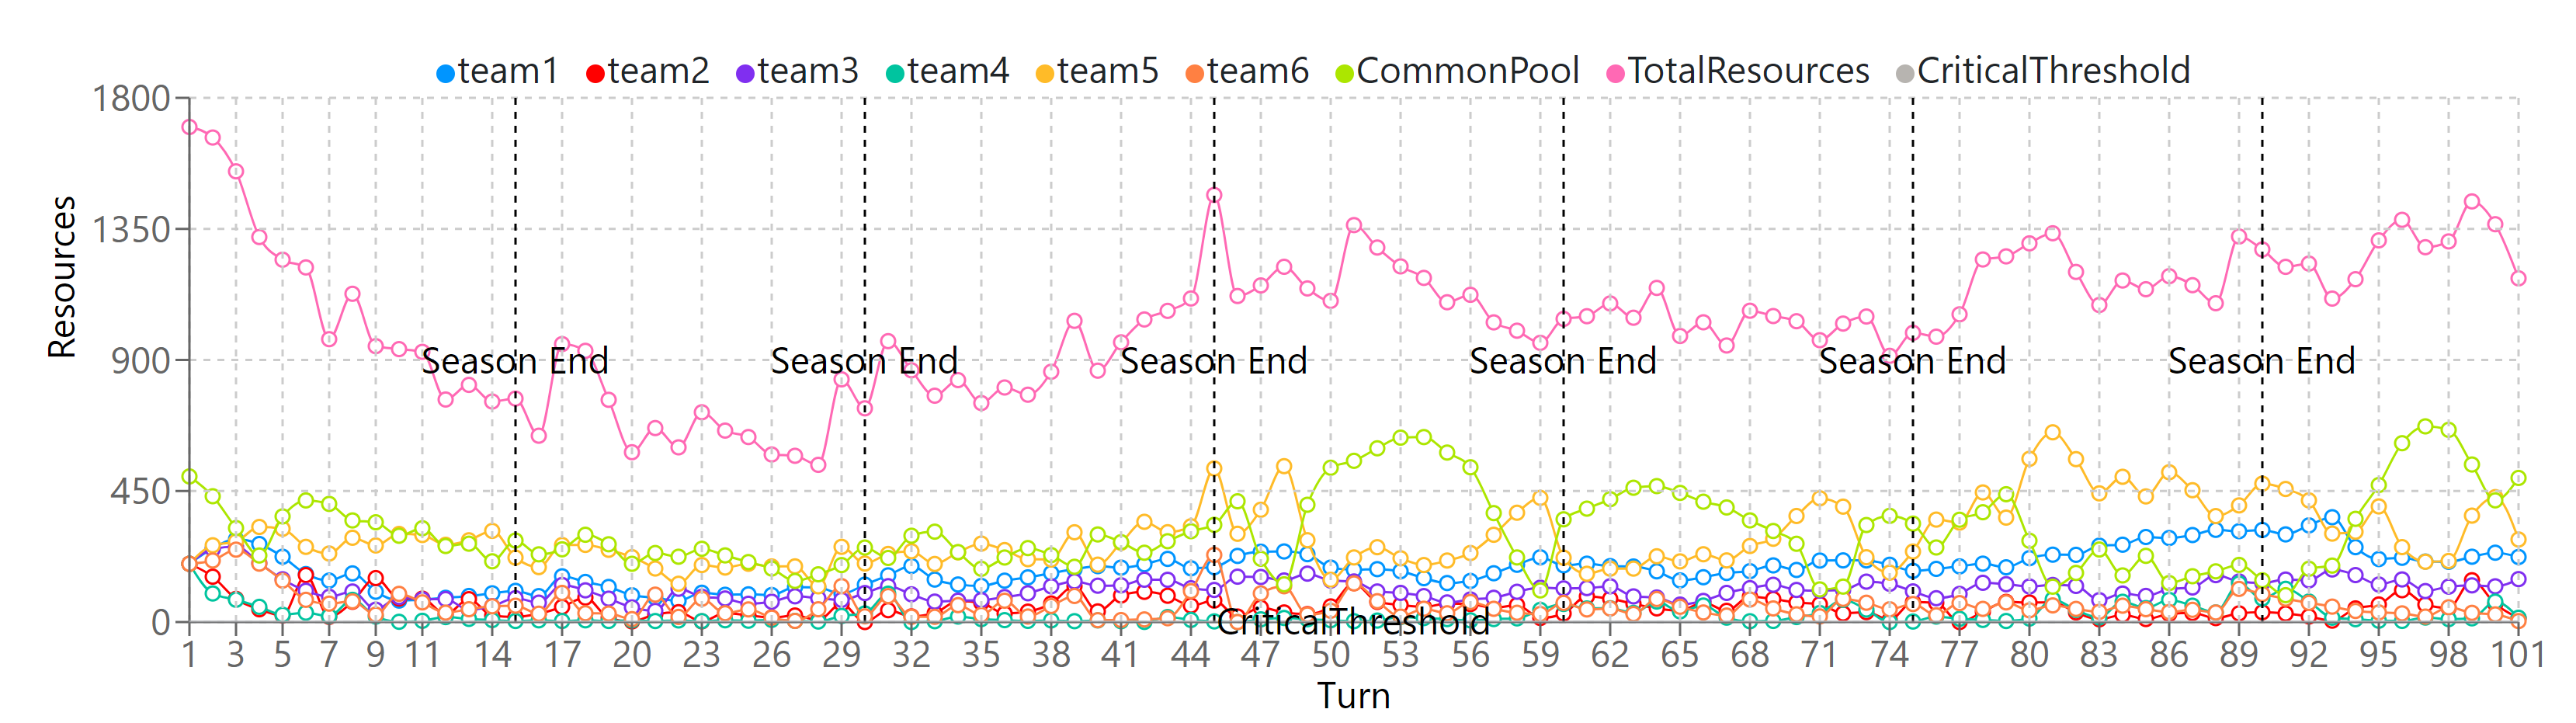
\includegraphics[width=0.9\textwidth]{13_team5_agentdesign/images/Agent Resources Inveserly correlated.png}
    \caption{Agent Resources Inversely correlated with the common Pool}
    \label{fig:Agent Resources Inversely correlated with the common Pool}
\end{figure}


We then altered the \texttt{MaxDeerPopulation} parameter for deer hunting with a input proportional\footnote{collective utility from the hunt is distributed proportionally to participants' contributions} resource return strategy. Our agent tend to live longer than in the baseline. However, with lower average resources.

Furthermore, the same parameter (\texttt{MaxDeerPopulation}) was tested for an equal utility distribution strategy. In this case, the agent's performs improved massively compared to the previously tested proportional distribution method: The agent became more generous with gifting and tended to survive considerably longer. Furthermore, the agent held more IIGO roles, which helped it accumulate more resources, allowing it to invest more into foraging.

When comparing the two methods of distribution, Figure~\ref{fig:Foraging Simulation MaxDeerpop_Prob} shows that the deer hunt is stable for both methods. However, For the equal distribution strategy as illustrated in Figure~\ref{fig:Foraging Simulation MaxDeerpop_Equal}, foraging activity increased substantially, as well as the foraging efficiency. 

\begin{figure}[!htb]
    \centering
    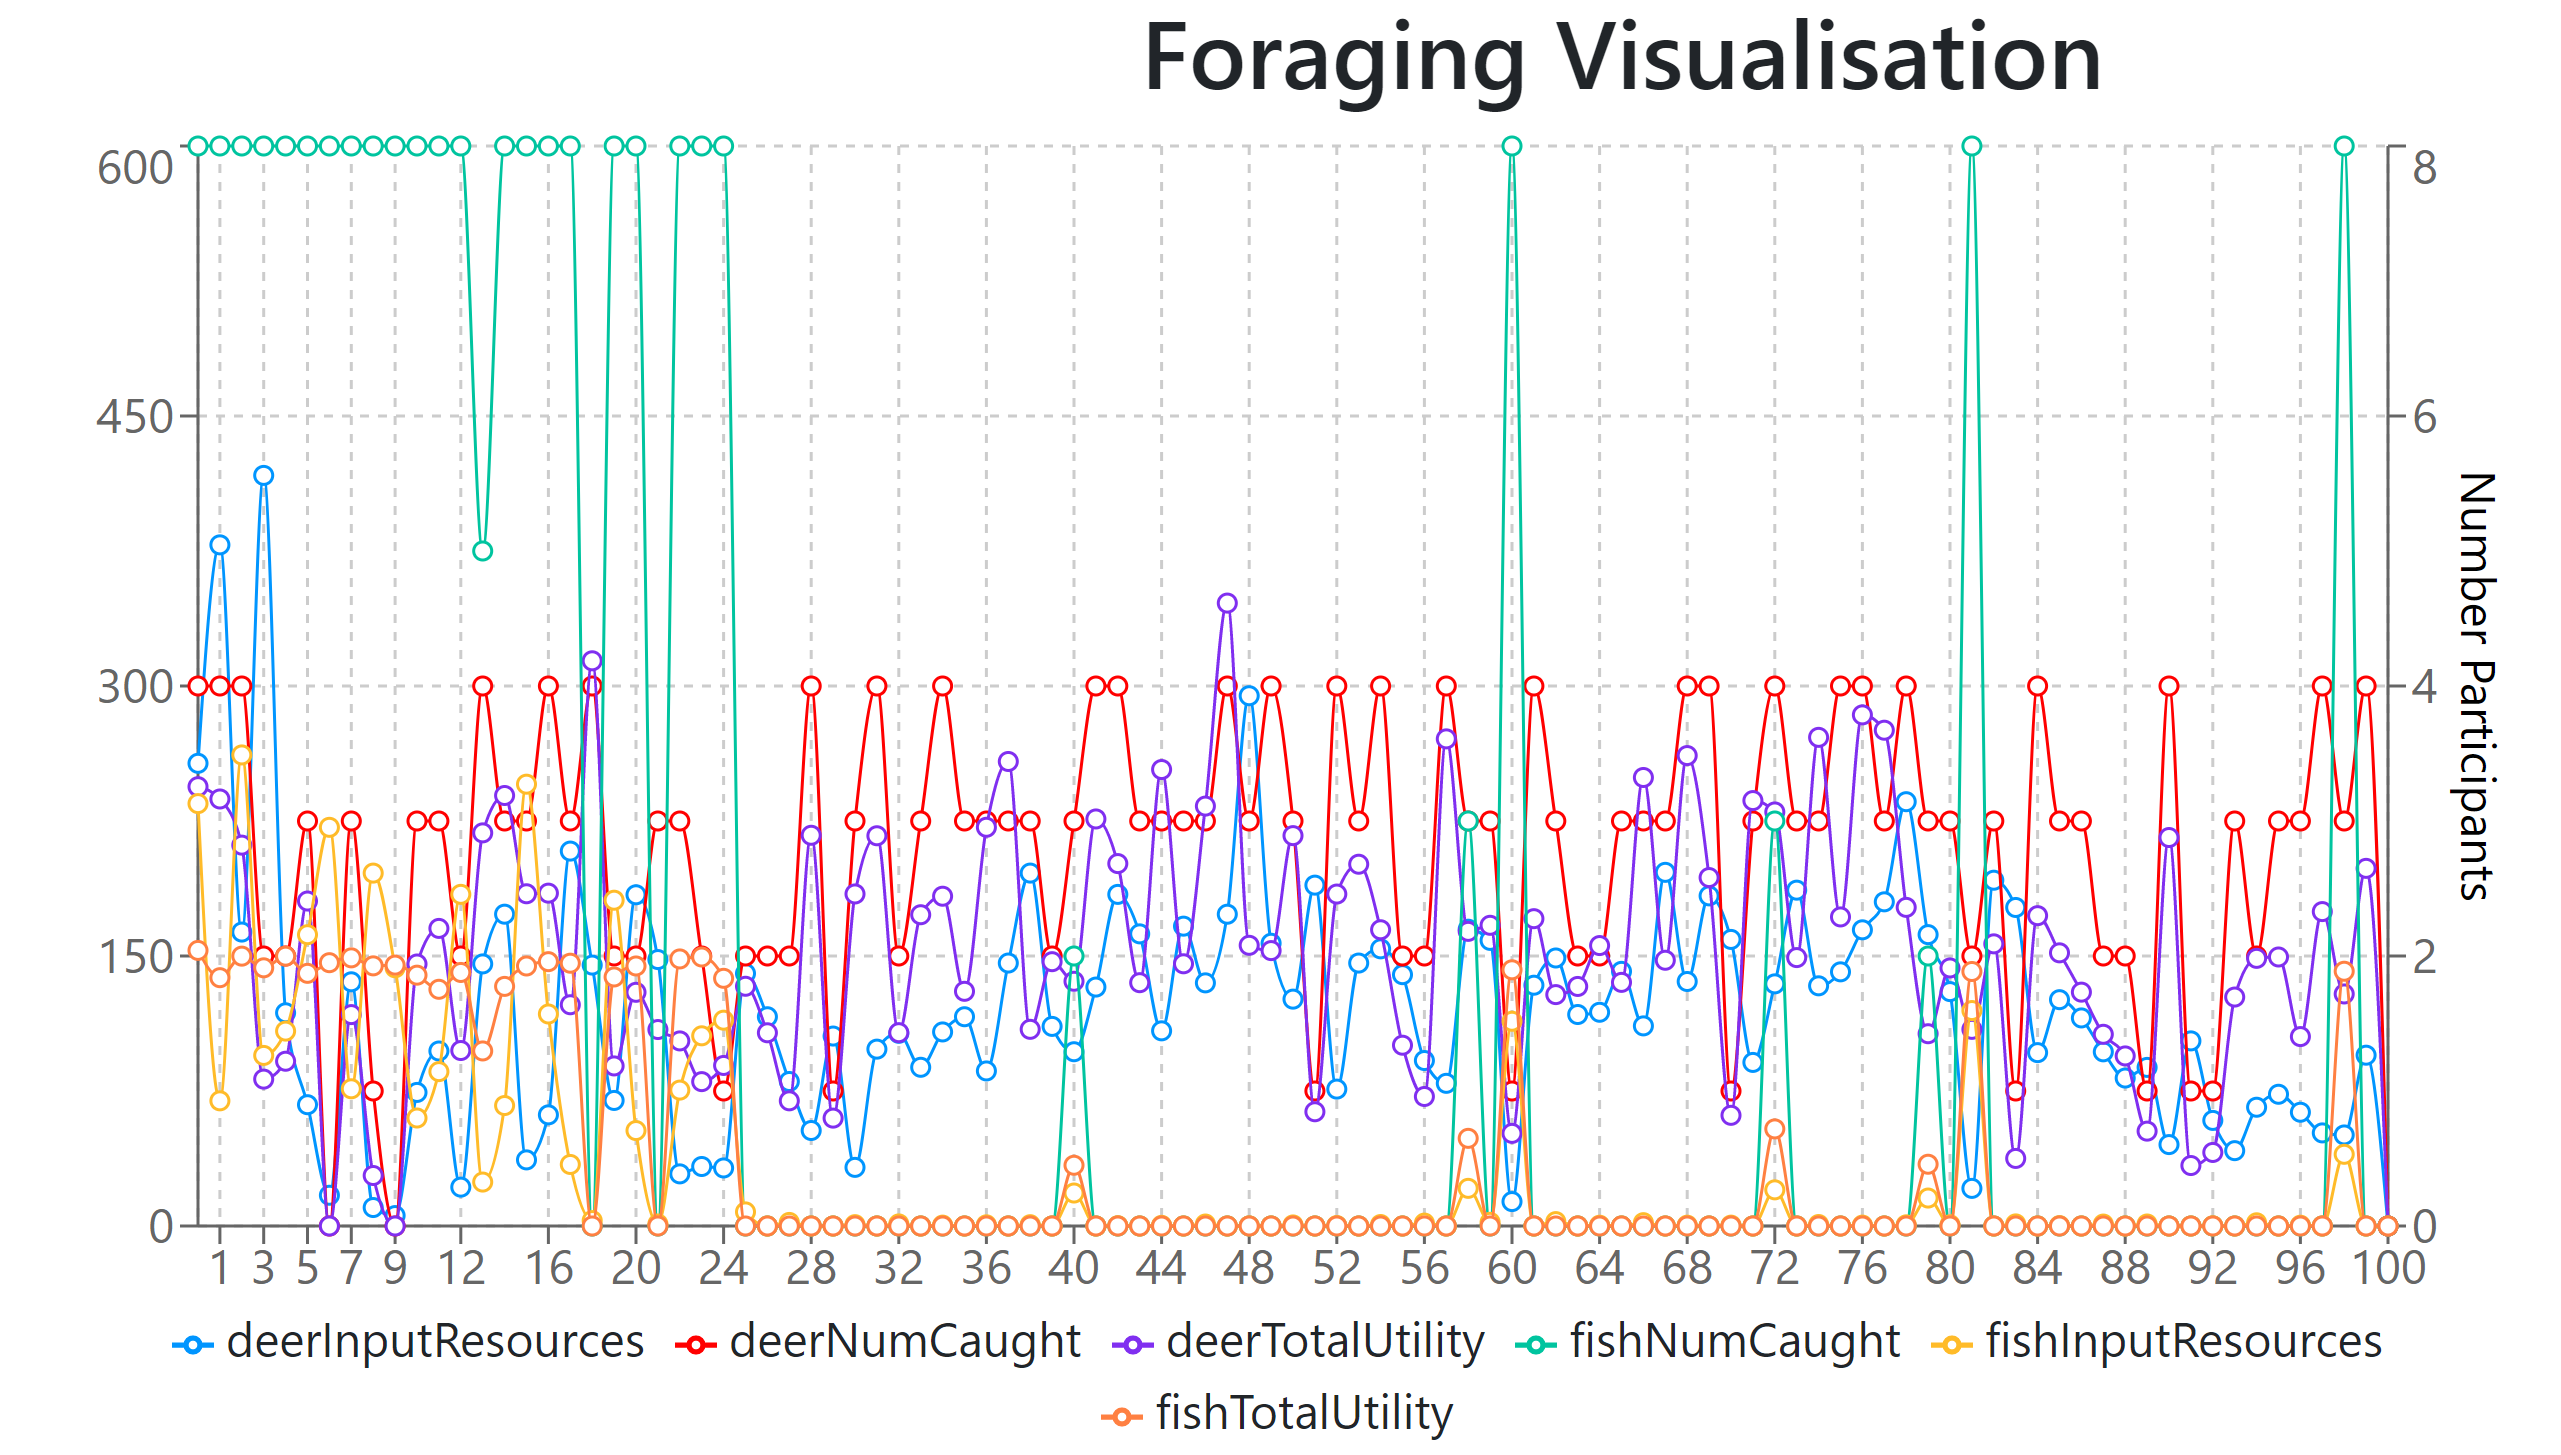
\includegraphics[width=0.8\textwidth]{13_team5_agentdesign/images/Foraging Simulation MaxDeerpop_Prob.PNG}
    \caption{Foraging Visualisation for a proportional distribution}
    \label{fig:Foraging Simulation MaxDeerpop_Prob}
\end{figure}

\begin{figure}[!htb]
    \centering
    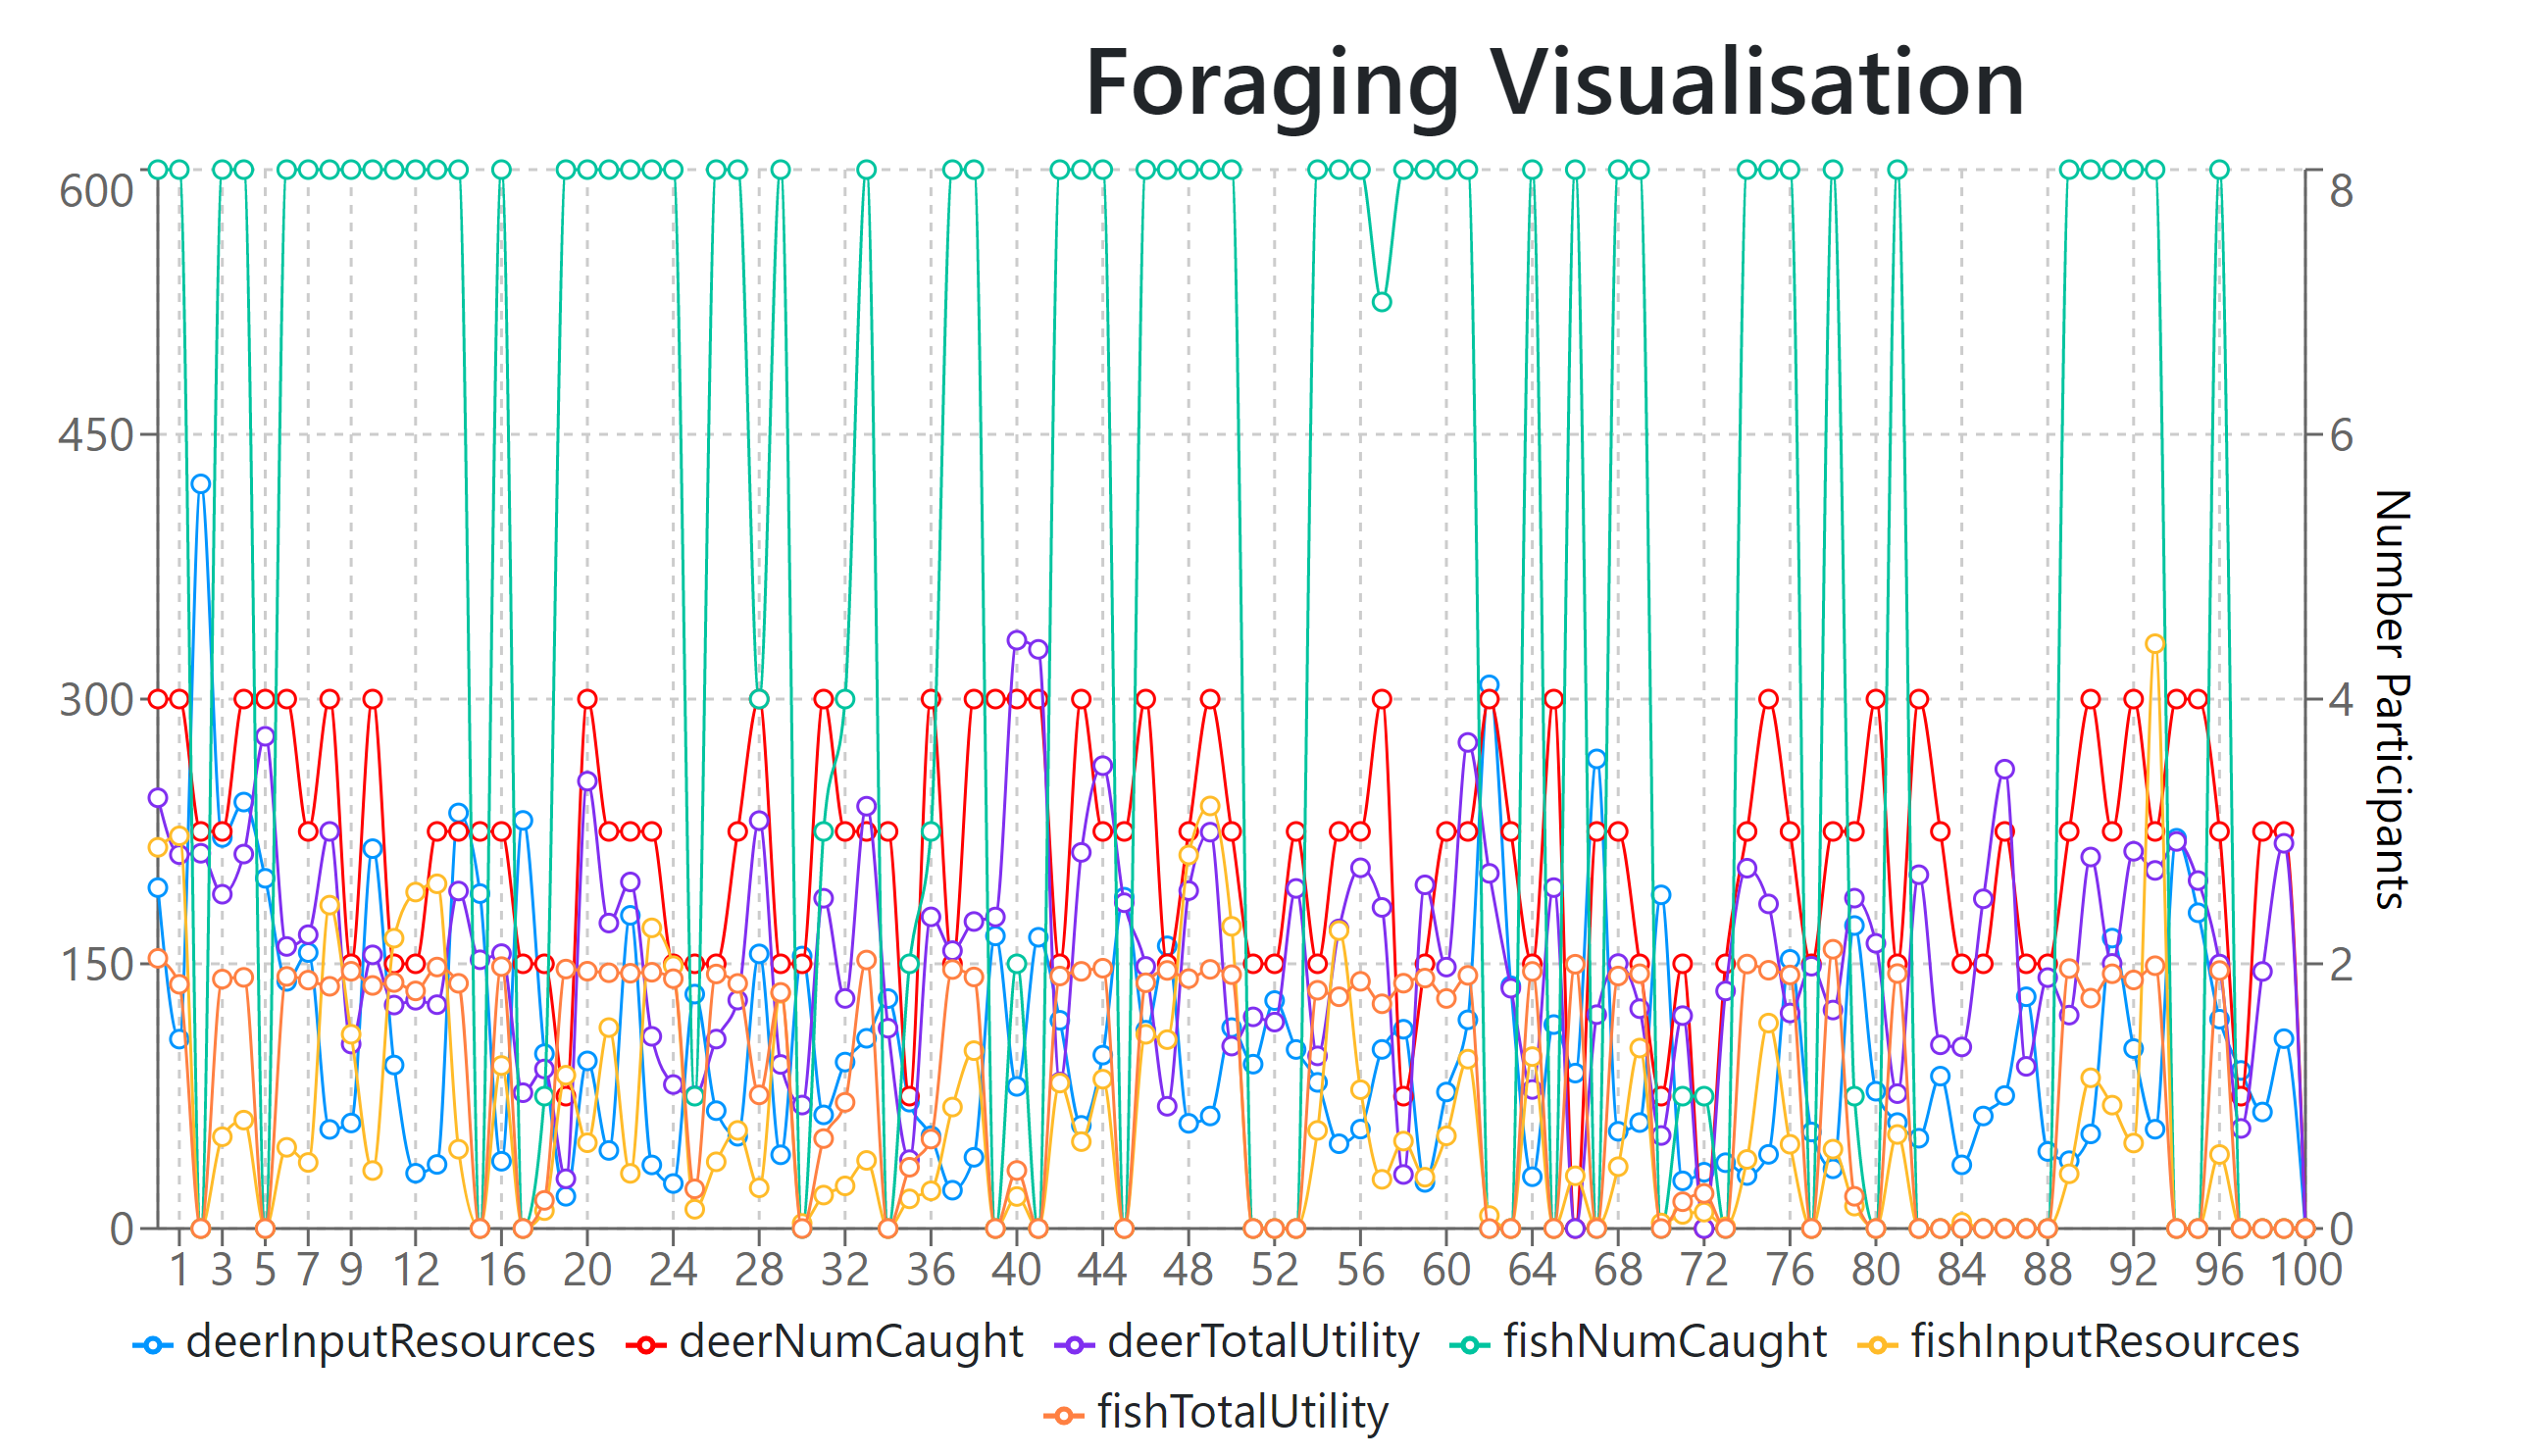
\includegraphics[width=0.8\textwidth]{13_team5_agentdesign/images/Foraging Simulation MaxDeerpop_Equal.PNG}
    \caption{Foraging Visualisation for an Equal distribution}
    \label{fig:Foraging Simulation MaxDeerpop_Equal}
\end{figure}

When the maximum deer population parameter in the game increases, the agent attempts to hunt as many deer as possible in a turn (as shown in Figure~\ref{fig:Foraging Simulation MaxDeerpop_Equal}, illustrated in the red line which is limited to a maximum of four deer that can be caught per turn). Whereas, when that parameter decreases, the agent reduces the amount of deer hunting and focuses more on fishing (Figure~\ref{fig:Foraging Simulation MaxDeerpop_Equal_decrease} - the green line represents the number of fish caught and the red line, the number of deer caught)

\begin{figure}[!htb]
    \centering
    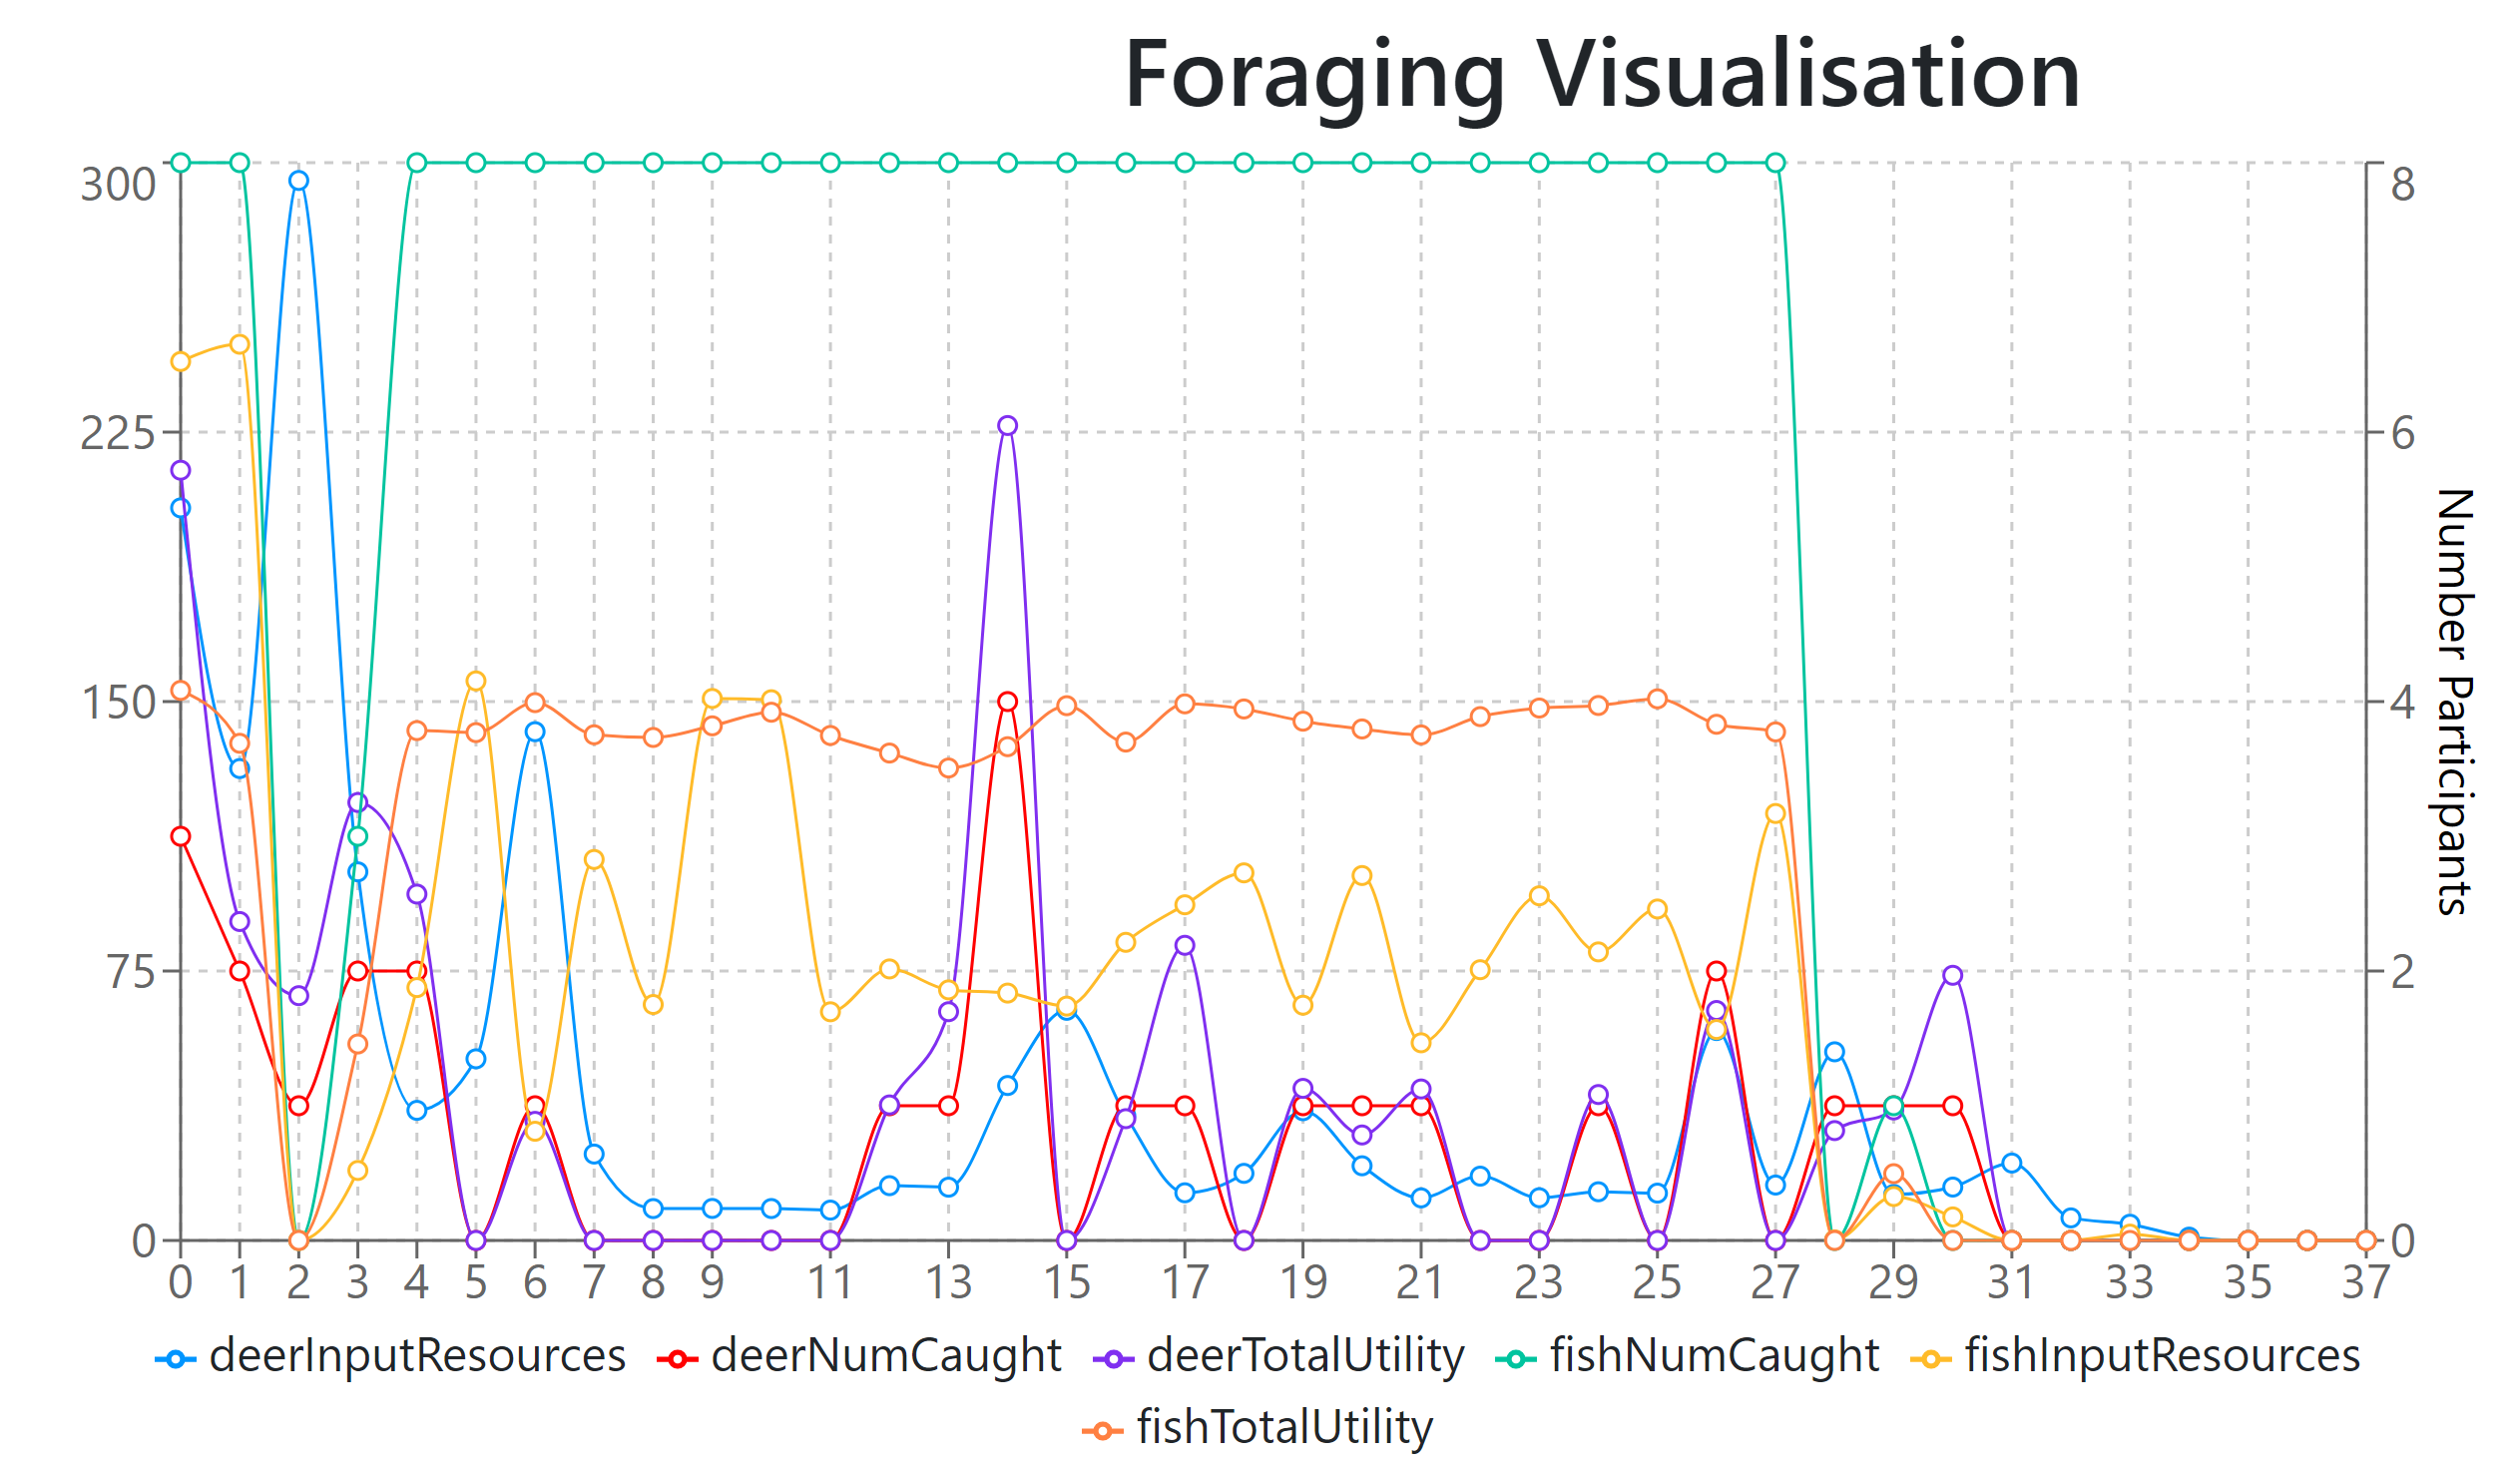
\includegraphics[width=0.8\textwidth]{13_team5_agentdesign/images/Foraging Simulation MaxDeerpop_Equal_decrease.PNG}
    \caption{Foraging Visualisation for an Equal distribution with a small Maximum Deer population Value}
    \label{fig:Foraging Simulation MaxDeerpop_Equal_decrease}
\end{figure}

It was spotted that our agent's tendency to over-invest into deer hunting. While the reward is high, the agent is over investing where lower contributions could lead to similar results.

Moreover, Fishing parameters have been altered to evaluate the behaviour and foraging efficiency of our agent. The simulated results are in Table~\ref{fig:Foraging Fishing parameters Simulation Results}.

\begin{figure}[!htb]
    \centering
    
\includegraphics[width=0.8\textwidth]{13_team5_agentdesign/images/Foarging Simulation Fishing.png}
    \caption{Foraging Fishing parameters Simulation Results}
    \label{fig:Foraging Fishing parameters Simulation Results}
\end{figure}

\texttt{MaxFishPerHunt} parameter represents the total number of fish that can be caught in a hunt. The simulation indicates our agent's fishing efficiency increases accordingly to an increase to the parameter. However, the deer hunting efficiency is very low. Therefore, our agent has no longer an incentive to go deer hunting as he could rather go fishing, which is a more reliable foraging method and guarantees a large return.

Our agent prefers high risk high reward approach. In order to survive, our agent invests a lot of his resources into deer hunting to gain a maximum amount of resources. However, this approach proves less favourable, as the simulation uncover that our agent do not recover from the "dying" state. Therefore, the reward dominant approach is not always the optimal strategy, and the agent should learn to switch to fishing.


\subsection{Disasters}
%% Disaster
The parameters examined in Figure~\ref{fig:DisasterParams} were evaluated using metrics we devised to evaluate the effect of changes in disaster parameters. 

\begin{figure}[!htb]
    \centering
    
\includegraphics[width=1\textwidth]{13_team5_agentdesign/images/Sim.png}
    \caption{Exploration of Disaster Parameters on Agent Metrics}
    \label{fig:DisasterParams}
\end{figure}

The effects of varying different parameters can be visualised in 
Figure~\ref{fig:DisasterParams}, where some metrics were devised for the evaluation of our agent. Foremost, we can see that the visibility of the threshold of the Common Pool influences how our agent interacts with other agents. Particularly, it was seen that when the threshold is visible, contributions to the common pool from our agent decreased with respect to the baseline. This resulted in more and larger transactions between our agent its counterparts. This could potentially be linked to the fact that our agent determines if threshold requirements are already met before contributing. Thus, a lower common pool contribution might encourage our agent to engage in other sorts of transactions. The effect of this is maximised when the threshold is lowered, leaving more resources to spend on other sorts of agent interactions and possibly, a higher contribution to foraging. For the latter, that might not be the case as it can be seen by the decrease of average resources when common pool threshold visibility is enabled. This is likely due to the hard cap on the maximum amount that our agent can invest in foraging or possibly due to the effect of other covariate parameters on the agent's foraging decisions.

Regarding adjustments to the \texttt{disasterPeriod} parameter, it can be seen that resource contributions and interactions with other clients increase by a proportionally larger amount when disaster period increases, i.e. disasters hit less often, implying that when our agent prospers, it tends to be more generous. This is a result of its opinion formation strategy. It is important to note that under multiple simulations, when the disaster period is visible, whether that is stochastic or not, the main metric that can be seen to be affected is the contribution to the common pool. 

However if we increase the \texttt{disasterMagnitudeResourceMultiplier} it can be observed that common pool contributions either increases or stays level to the baseline parameters. At the same time, transactions seem to be decreasing, showing that our island may be entering a “defense” mode, saving up for an upcoming disaster and ensuring that the common pool threshold is met. These observations are in favour of the proposed agent functionality.

The observations made using the above parameters, are dependent on other agent’s dynamics that were implemented. Therefore, without a collective analysis of each individual agents’ performance, conclusions are limited to the observations made solely under the specified experiment. One could only effectively evaluate an agent’s dynamics, taking in mind those of the rest of the agents in the community, given that they differ. Therefore, in future work simulations could be made with a community of only Team 5’s agent instances. Else, one would need to cross-reference the results from individual agent simulations, as well as results of simulating and evaluating the community as a whole. 

\subsection{Resource Management}

In the following experiments, we are testing the amount of the resources of our agent throughout the game. For each experiment, we were keeping all the parameters fixed to baseline and adjusting only one to analyse it would affect our agent overtime. 

\underline{Parameter:} Initial Common Pool \newline
\underline{Agent Baseline Value:}1000 \newline
\underline{Tested values:} \{120, 2000, 0, 200\} \newline
\underline{Observation:} \newline
We have observed that our agent performs better in comparison to the rest when the amount of resources in the common pool is limited. This is because our agent's behaviour is not competitive and it does not request great amounts of resources if its state is not critical, while other agents often seem to exploit the common pool. An exceptional scenario is when the initial resources are too low and the agents does not manage to recover from the first disaster.
Below, there are two Figu that are representative of our agent's performance in comparison to the other agents when initial common pool is high and when it is low.

\begin{figure}[!htb]
    \centering
    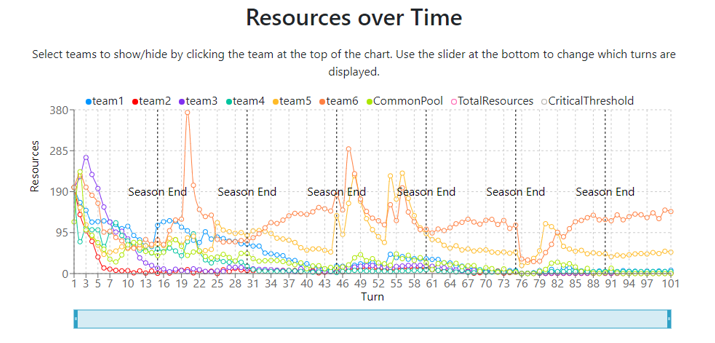
\includegraphics[width=0.6\textwidth]{13_team5_agentdesign/images/InitCP120.PNG}
    \caption{Initial Common Pool: 120}
    \label{eq:Initial Common Pool: 120}
\end{figure}

\begin{figure}[!htb]
    \centering
    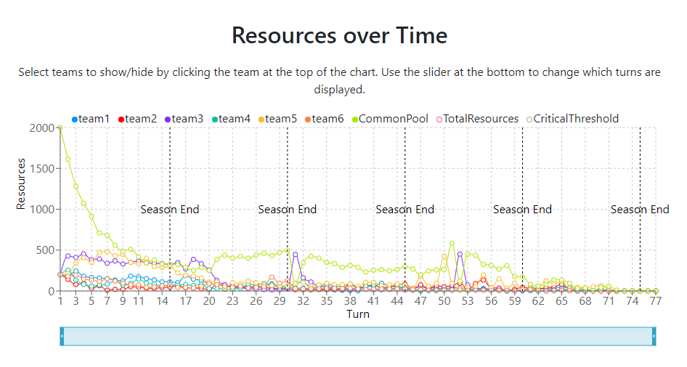
\includegraphics[width=0.6\textwidth]{13_team5_agentdesign/images/InitCP2000.PNG}
    \caption{Initial Common Pool: 200}
    \label{Initial Common Pool: 200}
\end{figure}

\underline{Parameter:} Initial Resources \newline
\underline{Agent Baseline Value:}200 \newline
\underline{Tested values:} \{50, 500, 1000\} \newline
\underline{Observation:} \newline
What was observed in these experiments is that our agent is ignorant to the initial amount of resources. More specifically, no matter what the initial resources, our agent's resource level stabilises after some number of turns. Our agent is designed to have a sophisticated foraging strategy and thus, its survival does not depend on the given resources or the common pool. The graph below illustrates this.

\begin{figure}[!htb]
    \centering
    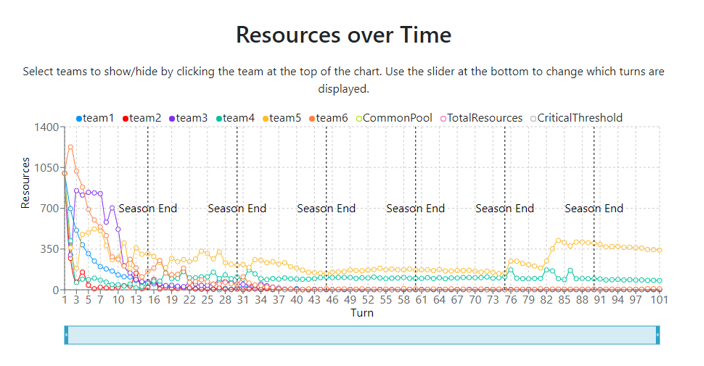
\includegraphics[width=0.6\textwidth]{13_team5_agentdesign/images/InitRes.PNG}
    \caption{Initial Resources of agent: 1000}
\end{figure}


\underline{Parameter:} Cost of Living \newline
\underline{Agent Baseline Value:}5 \newline
\underline{Tested values:} \{100, 50, 1, 10\} \newline
\underline{Observation:} \newline
The results of these experiments where similar to the ones of the previous experiment. Our agent survives and arrives in a state of equilibrium independently of the cost of living, as long as it is not extremely high; $\approx$ 100.

\underline{Parameter:} Maximum Number of Turns \newline
\underline{Agent Baseline Value:}100 \newline
\underline{Tested values:} \{200, 300\} \newline
\underline{Observation:} \newline
In this trial, our aim was to test the longevity of our agent. We observed that in all the experiments our agent managed to remain alive. Following to what has been described above, our agent develops a sustainable strategy that assures its survival and persistence. Additionally to that, we observed that after the leave of some agents, the whole environment becomes more stable and the remaining agents manages to maintain a fixed amount of resources. A possible explanation could be that the environmental parameters such as available resources etc. are not sufficient to satisfy six islands.
\newline
\textit{Note: We also tested multiple combinations of the values of the parameters \texttt{minimumResourceThreshold} and \texttt{maxCriticalConsecutiveTurns} but since our agent manages to maintain a sufficient amount of resources throughout all the turns of the baseline scenario, it is not affected by these parameter - as long as they remain in a reasonable value.}

















\subsection{Discussion}

Overall, our agent has a set of different actions to take depending on how other islands interact with it. It is interesting to see how the agent's behavior constantly changes in simulations even without any change in the game's parameters.Given more time, it would be interesting to incorporate personality behaviour such as altruistic and selfish according to our wealth tiers. Furthermore having these internal personalities change as the game progresses or when certain roles are achieved. 



%\section{\appendixautorefname{}}
%\lstinputlisting[language=go]{configbaseline.go}





    \chapter{Team 6 Agent Design}
\section{Introduction} \label{sec:Team6_Intro}
Our agent/island, which is on behalf of one of the islands sitting on the archipelago, has some basic properties controlling the overall behaviour. Three main properties includes \emph{Personality}, \emph{Friendship} and \emph{Trust Rank}. \emph{Personality} implicitly refers to the amount of the resources our island currently holds. There are three tiers of personality, each makes our island perform different actions during the interaction with other islands. The more resources we have, the more generous our island is. \emph{Friendship} is a map containing keys as islands and values as the friendliness with certain island. It measures the relationship between our islands and the others, and can be either increased or decreased. The changes happens mostly at the IITO session of each turn, when the gifts are exchanged. For example, if the total amount of gifts we have received from an island is less than the amount of gifts we sent to an island, the friendship level with that island will be reduced by how much the difference between our gifts. \emph{Trust Rank} determines how much our island can trust an island. It is then used to Judge the way we consider their prediction of a disaster in the IIFO session. For islands holding less trust rank with us, their prediction results will be applied with a weight factor that heavily penalises the result. The final prediction for IIFO is the mean value of the predictions from all 6 islands.

\section{Design and Implementation} \label{sec:Team6_design_impl}

\subsection{IIGO} \label{subsec:Team6_IIGO}
In IIGO session, besides the collaboration of three distinct branches to maintain, update and revise the rule, decision regarding allocation request from common pool is made by each agent. Agents are required to act in this session based on their resources availability. The decision-making actions which are required from each island are:
\begin{itemize}
    \item contribute resources to the common pool in form of taxation which is the minimum amount set by the President.
    \item request resources from the common pool.
    \item vote in favor/against the proposed rule made by the President.
    \item vote in the election of Judge, Speaker, and President.
\end{itemize}
There are two potential problems that could arise in this situation:
\begin{itemize}
\item an agent can request resources much more than necessary. As a result, there are not enough resources in Common Pool for other agents to request, i.e., agents lose the opportunity to generate resources and have less ability to participate in foraging. Therefore, agents will get less return from foraging. This problem follows the notion of micro-level goal, which states that a self-interested agent will try to satisfy maximally; and also the concept of the tragedy of the common proposed by Gerit Hardin, which says that people will make a decision that maximises their interests in the short term, even if this leads to the deterioration of the common pool resource in the long run, which is in nobody's interest~\footnote{Pitt, J. \textit{Self-Organising Multi-Agent Systems} (p. 156). IC Press.}.
    \item an agent requests too few of resources, as there are not sufficient resources in the Common Pool. This also has a negative effect on agent’s ability to invest in foraging. Consequently, the agent will less likely to survive. 
\end{itemize}

\subsubsection{Strategies} \label{subsubsec:Team6_IIGO:Strategies}
Our agent has the personality which is based on the current amount of resources. The personality parameter is a dynamic variable that is adjustable, and helps assisting agent’s decision in any event related to economic aspect. These personalities consist of normal, selfish, and generous. This parameter is used to determine whether or not we would like to request resources from the common pool. 

\subsubsection{Implementation} \label{subsubsec:Team6_IIGO:Implementation}
\begin{itemize}
\item \textbf{Request Allocation}: when the current resource is below the minimum threshold, the difference of minimum threshold minus current resource will be requested. If the current resource is above threshold, the request will depend on the personality. If the allocation amount determined is not enough for living cost and the current personality is selfish, the agent will take the amount equals to living cost. In other situations, only the resources allocated will be taken.
\item \textbf{Common Pool Resource Request}: when our island is not in critical status and the current resource is larger than the minimum threshold, the common pool resource will be requested based on the personality. In generous mode, our agent will only ask for living cost of one day, otherwise we will ask for three times of the living cost. However, more resources allocated means more contribution in foraging and can bring abundant return and subsequently abundant tax will be paid after.
\item \textbf{Tax Contribution}: in normal situation, the exact tax amount determined by the President will be paid. However, no tax will be paid if we are in critical status. When the disaster is approaching (our prediction for the time left $< 1$) and the current personality is generous, more tax will be paid. 
\item \textbf {Sanction Payment}: sanction will be paid if our island is not in critical status. If our resource can be lower than the minimum threshold after paying the determined sanction amount, then we will try to only pay partially above the threshold. 
\item \textbf {Resource report}: when the personality of the agent is selfish, only a half of the actual resource will be reported in order to get more allocation.
\end{itemize}
%\subsubsection{Opinions}

\subsection{IITO} \label{subsec:Team6_IITO}
\subsubsection{Trust and Relationship Dilemma} \label{subsubsec:Team6_IITO:Dilemma}
In IITO sessions, communications and interactions among the islands/agents happen during the game to exchange information, besides governance-related information which happens in IIGO sessions, with details mentioned in Subsection~\ref{subsec:IITO:inter_island_communication}. The highlight for agent strategy in IITO sessions is especially related to the actions of giving and receiving gifts to/from other island(s) in terms of resources. Islands are required to act in this session based on the resource information of their own private pool and/or of other island's if available (i.e. islands are willing to share resource information to other islands).

As described in Subsection~\ref{subsec:IITO:gifting_session}, the decision-making actions that are required from the island are, whether the island wishes to:
\begin{itemize}
    \item request gifts of certain amount of resources from specific island(s).
    \item offer gifts of certain amount of resources to specific island(s).
    \item respond to gifts of certain amount of resources offered to them from the other island(s), provided some available choices i.e. to accept the full amount of the offered gifts, to accept partial amount of the offered gifts, or to decline the offered gifts.
    \item update the history of the above three events (including the amount) to be informed to the respective island(s).
\end{itemize}

The potential emerging dilemma in this part is related to decision-making under uncertainty from social construction of the agents' social interaction. In this context, the concept of \emph{trust} is introduced as a key factor in the social relations. According to the trust framework~\footnote{Pitt, J. \textit{Self-Organising Multi-Agent Systems} (pp. 234-235). IC Press.}, there are three aspects that affect the perspective of one's decision-making in social relations:
\begin{itemize}
    \item cognitive dimension: beliefs, interpretation of signals, etc.
    \item economic dimension: utility, cost/benefit analysis, etc.
    \item normative dimension: rule, expectation of conformance or punishment for non-compliance, etc.
\end{itemize}
We mainly focus on the economic dimension as it is the measurable parameter in the game that is helpful for the decision-making.

\subsubsection{Strategies} \label{subsubsec:Team6_IITO:Strategies}
Based on the economic dimension for decision-making as mentioned in the above, our agent strategy for taking actions on this gifting mechanism is parameterised by the following aspects:
\begin{itemize}
    \item current status of our island and other islands at current state of the game, i.e. alive, critical or dead, including the counter of the critical status (how many turns stay in critical status).
    \item chosen personality mode of our island at current state of the game, i.e. selfish, normal or generous.
    \item current resource level in our island's private pool with some considered factors such as a minimum threshold for disaster coverage, and the cost of living.
    \item level of friendship between our island and the other island(s) correspondingly by using friendship coefficient.
\end{itemize}
For requesting gifts from other island(s), firstly we do not request for any gift from the island(s) that is/are not alive at the state of the game. Then, in order to survive the game, our island submit the request to all islands if we are in critical status (current resource level is less than the minimum threshold) with the value requested is the amount of minimum threshold. Otherwise, if our island is not in critical status, we would still submit request for gifts to other islands, but it depends on the personality mode we are playing at the state of the game that proportional to a multiplier factor (\emph{friendship coefficient}) to the value of cost of living.

For offering gifts to other island(s), firstly we do not offer any gift to any other islands if we are in the critical status at the state of the game, as this is part of the self-preservation mechanism of our own resource level to survive. Secondly, we prioritise the other islands who are in critical status, thus we offer them a minimum threshold value of resources to help them survived, as part of the common goal for sustainability of the archipelago. Otherwise, for non-critical circumstances, the strategies depend on the friendship level and the chosen personality of our own island. Friendship level sorts out on the preference which island we offer the gift to with the proportion amount of resources that do not make our island goes to critical level. Meanwhile, the chosen personality of our island introduces a penalty factor to the gift offers we received by using the friendship coefficient. When we are generous, no penalty is used, thus our island accept the received offers given to us.

For gifts responses, firstly we just accept all gifts of the offered amount of resources from any island if we are in the critical status. Otherwise, we also just decline the offered gifts from islands that are in critical status to save their resources. Under normal circumstances, our island responds to the gifts from other islands based on the friendship level, i.e. decline it when the island has minimum level of friendship with our island, or accept it partially (with the deduction of cost of living) when the island has maximum level of friendship with us.

\subsubsection{Implementation} \label{subsubsec:Team6_IITO:Implementation}
The gift exchanging is the main activity during the IITO session where each island exchanges some of their resources, known as \emph{gift}, with the other islands. The behaviour of our island for gifting will be controlled by two of our main properties: \emph{Friendship} and \emph{Personality}. In general, the less resources we have in our private pool, the more egocentric our island will be. Nevertheless, in each turn of the IITO session, there are some extra checking to be done before performing our specific behaviour based on these properties. Firstly, if we find our island is in the critical status, which means we are going to die in a few turns to come, we will instantly decide that there will be no gift to be sent to anyone in this round. Otherwise, there will be gifts from us sent to other islands. The islands in critical status hold the privilege to certainly receive a few amount of gifts from us in order to help them out of the critical status, as we bear in mind the fact that the maximum chance of survival of any single island depends on the survival of all islands. After checking these priorities, we then determine what gifts we send to the other islands in non-critical status.
\begin{algorithm}[H]
\SetAlgoLined
    \uIf{Personality == Selfish}{
        request gifts scaled up by friendship coefficients\;
    }
    \uElseIf{Personality == Normal}{
        request gifts without scaling\;
    }
    \uElseIf{Personality == Generous}{
        request gifts scaled down by friendship coefficients\;
    }
    \caption{Gifts Requests}
\end{algorithm}

\begin{algorithm}[H]
\SetAlgoLined
    \uIf{Personality == Selfish}{
        request gifts scaled down by friendship coefficients\;
    }
    \uElseIf{Personality == Normal}{
        request gifts without scaling\;
    }
    \uElseIf{Personality == Generous}{
        request gifts scaled up by friendship coefficients\;
    }
    \caption{Gifts Offers}
\end{algorithm}


The algorithm above concludes how our agent makes use of Friendship and Personality, and behaves differently during the gift exchanging section. Basically, the amount of any gifts can be linearly scaled based on how much friendship we have with the target island whom we are requesting or offering gifts to. For example, if our island is \emph{selfish}, the amount of the gift we offer will be scaled down by a value depending on the current friendship. A relative coefficient will be calculated based on that. If the island is a good friend with us, the coefficient will be relatively lower when it comes to the gift offers, so that the amount by which it is scaled down will be less. Otherwise, the coefficient will be higher and a higher penalty will be applied so that we offer our bad friend very few gifts.
%\subsubsection{Opinions}

\subsection{IIFO} \label{subsec:Team6_IIFO}
\subsubsection{Long-Term Collective Risk Dilemma} \label{subsubsec:Team6_IIFO:ltCRD}
% Individual utilities vs CPR
Our agent faces a cost of living deducted at every turn, and an expenditure when a disaster hits. To mitigate the effect of disaster, islands make contributions to the common-pool. The long-term collective risk dilemma (ltCRD) defines that how much resources are needed to be raised and before when. We parameterise such problem with a threshold $T$ and a deadline day $D$.


\subsubsection{Strategies} \label{subsubsec:Team6_IIFO:Strategies}
In this coursework, there are non-stochastic and stochastic disasters. For the non-stochastic disaster, $T$ is known and $D$ is unknown. For the stochastic disaster, both $T$ and $D$ are unknown. To deal with ltCRD, the islands make forecast about $T$ and $D$, whereas each island has its own knowledge to predict the disaster. On the one hand, when an individual island forms an opinion regarding the desired contribution to the common-pool resources, it is necessary to convince others that the decision is rational. On the other hand, we take the aggregate knowledge into consideration, taking advantages of distributed computation of disaster prediction. Such prediction information comprises:
\begin{itemize}
    \item the coordinates.
    \item the magnitude of disasters.
    \item the confidence of prediction.
\end{itemize}
The recommendation of common-pool resource contribution is based on the comparison among our own prediction and shared predictions from others. 

\subsubsection{Implementation} \label{subsubsec:Team6_IIFO:Implementation}
For the foraging, islands can share the most recent foraging decisions they made and the resources obtained to other islands. There is a \texttt{ShareTo} list containing island IDs that our island wishes to share this information with. The following pseudocode describes the logic in our disaster prediction:
\begin{algorithm}[H]
\SetAlgoLined
    \uIf{not knowing the period \textbf{and} not knowing whether it's stochastic}{
        check the disaster history\;
        find if it is stochastic\;
        find the disaster period\;
    }
    \uElseIf{knowing the period \textbf{and} not knowing whether it's stochastic}{
        check the disaster history\;
        find if it is stochastic\;
    }
    \uElseIf{not knowing the period \textbf{and} knowing whether it's stochastic}{
        check the disaster history\;
        find the disaster period\;
    }
    decide the prediction based on the period and stochastic information we have\;
    \caption{Disaster Prediction}
\end{algorithm}


Since the coordinates of a happening disaster follows a uniform distribution which makes it totally random and unpredictable, our island focuses the prediction on the time left for a disaster to happen in different ways based on whether or not the settings of period and stochastic disaster is exposed. It is possible to calculate the exact time of a disaster if it is not stochastic. Otherwise, the possibility of a disaster can be calculated based on the period if it is stochastic. For either case, it is assumed that the period and the stochastic condition are exposed to our agent. However, chances are that one or both of these settings are not exposed to us. In this case, our agent will look through our disaster history and try to find the settings based on the patterns. For example, if the agent finds the time period between any two disasters is not identical, then it will reckon the disaster period to be stochastic. Otherwise, if it find all the period between any of the two disaster is the same, the agent will consider the setting of disaster is not stochastic, where there is a fixed period between the disasters. Based on the final prediction we have made, our island will determine how much resources we want to invest to the common pool to mitigate the disaster impact.

%\subsubsection{Opinions}

\subsection{Foraging} \label{subsec:Team6_Foraging}
\subsubsection{Risk-Payoff Dilemma} \label{subsubsec:Team6_Foraging:RP_dilemma}
In each turn, our agent has an opportunity to gain resources from the environment by foraging. Such action can be regarded as an investment of resources by deciding:
\begin{itemize}
    \item the type of foraging i.e. either deer hunting or fishing.
    \item the quantity of resources that our agent invests.
\end{itemize}
The consideration of risk and payoff underpins the rationale of decision-making. Within the context of this coursework, deer hunting offers a high amount of payoff with high risk, whereas fishing is a low-risk decision with relatively lower returns. The dilemma of risk and payoff has been studied in Stag Hunt Game~\footnote{Pitt, J. \textit{Self-Organising Multi-Agent Systems} (pp. 84-85). IC Press.}, where the difference of outcome between the safe option and the risky option affects the preferable choice. By introducing return on investment (ROI) regarding the total investments on deer hunting and fishing, our agent can estimate the difference between safe and risky investments.

\subsubsection{Inter-Foraging-Group Dilemma} \label{subsubsec:Team6_Foraging:Group_dilemma}

According to Kitchen Stand-Off game~\footnote{Pitt, J. \textit{Self-Organising Multi-Agent Systems} (pp. 67-68). IC Press.}, social welfare can be maintained by not necessarily the cooperation, while a huge individual contribution can unilaterally support it. In this coursework, the quantity of investments from individual agents foraging together determines the level of return. In fishing, the return to all participants is equally distributed as long as the total investment reaches a certain value. This brings out the dilemma between individual contribution and collective return. 

Table~\ref{table:FishAbundant} and~\ref{table:FishScarce} presents the possible outcomes introduced by the decision on fishing. 

\begin{table}[!htb]
    \setlength{\extrarowheight}{2pt}
    %\centering
    \begin{tabular}{cc|c|c|}
      & \multicolumn{1}{c}{} & \multicolumn{2}{c}{Other Agents' Total Investment}\\
      & \multicolumn{1}{c}{} & \multicolumn{1}{c}{$Low$}  & \multicolumn{1}{c}{$High$} \\\cline{3-4}
      \multirow{2}*{Our Agent's Investment}  & $Low$ & $(1,1)$ & $(2,4)$ \\\cline{3-4}
      & $High$ & $(4,2)$ & $(3,3)$ \\\cline{3-4}
    \end{tabular}
    \caption{Decision Matrix - When the population of fish is abundant.}\label{table:FishAbundant}
\end{table}

\begin{table}[!htb]
    \setlength{\extrarowheight}{2pt}
    %\centering
    \begin{tabular}{cc|c|c|}
      & \multicolumn{1}{c}{} & \multicolumn{2}{c}{Other Agents' Total Investment}\\
      & \multicolumn{1}{c}{} & \multicolumn{1}{c}{$Low$}  & \multicolumn{1}{c}{$High$} \\\cline{3-4}
      \multirow{2}*{Our Agent's Investment}  & $Low$ & $(1,1)$ & $(0,2)$ \\\cline{3-4}
      & $High$ & $(2,0)$ & $(0,0)$ \\\cline{3-4}
    \end{tabular}
    \caption{Decision Matrix - When the population of fish is scarce.}\label{table:FishScarce}
\end{table}
\subsubsection{Strategies} \label{subsubsec:Team6_Foraging:Strategies}
Backtracking foraging history allows us to monitor the trend of ROI and capital input. The qualitative opinion formation is based on historical foraging information exchanged in IIFO session: 
\begin{itemize}
    \item overall resource input to foraging increases, which indicates that the high-tier foraging return is likely to obtained. In such case, increasing our input is preferred.
    \item overall resource input to foraging decreases, which indicates that the low-tier foraging return is likely to obtained. In such case, reducing our input is preferred.
\end{itemize}

The quantitative decision regarding the amount of investment refers to the amount that we invested in previous turns. Such amount of extra input or less input is determined by our current personality. Referring to the decision matrix~\ref{table:FishAbundant} and~\ref{table:FishScarce}, we gain more benefits when the overall investment is high and our investment is lower than others. This implies a high efficiency of foraging from our perspective. However, if the gap between the average of total investments and ours is large enough, it will not be sustainable for other islands due to their relatively lower foraging efficiencies. Hence, we follow:
\begin{itemize}
    \item when the overall resource input to foraging increases, we increase the investment but not higher than the average of investment, which is estimated by historical overall investments.
    \item when the overall resource input to foraging decreases, we decrease the investment or consider changing the foraging type.
\end{itemize}


\subsubsection{Implementation} \label{subsubsec:Team6_Foraging:Implementation}
There is a map that records all the forging history. Our agent will do two deer hunting and one fish hunting at the first three rounds, as there are insufficient items in the map for running the algorithm. Contribution to the foraging is calculated by using a multiplier for the value of current amount of our resources minus safety buffer. The safety buffer is calculated by adding the Cost of Living and the Minimum Resource Threshold, which are determined in the server. The multiplier is adjusted by analysing the ROI (Return on Investment) trending. The multiplier will be larger if the trending is increasing, and will be smaller otherwise.

The forging type for current turn is decided by comparing the average ROI of total deer hunting with the total fishing from the last turn. The one with better average ROI will be chosen.

\begin{algorithm}[H]
\caption{Foraging} 
    %\begin{algorithmc}
    calculate the average ROI for deer hunting last turn $\alpha_1$\;
    calculate the average ROI for fish hunting last turn  $\beta_1$\;
    calculate the average ROI for deer hunting 2 rounds before $\alpha_2$\;
    calculate the average ROI for fish hunting 2 rounds before $\beta_2$\;
    \If{$\alpha_1 > \beta_1$}{
        \If{$\alpha_1 > \alpha_2$}{$multiplier \gets multiplier + 0.05$\;}
        \Else{$multiplier \gets multiplier - 0.05$\;}
        \Return deer type\;
    }
    \Else{
        \If{$\beta_1 > \beta_2$}{$multiplier \gets multiplier + 0.03$\;}
        \Else{$multiplier \gets multiplier - 0.03$\;}
        \Return fish type\;
    }
    %\end{algorithmc}
\end{algorithm}

Since fishing is a safer choice than deer hunting, the sumand used in deer hunting will be larger than that in fishing. The general idea for this algorithm is to calculate the differential of the total ROI history curve. Due to time limit, the difference value between the last round and 2 rounds before is used to replace the differential.

\subsection{President} \label{subsec:Team6_President}
\subsubsection{Individual taxation problem} \label{subsubsec:Team6_President:Dilemma}
In each turn, the President has the power to decide the taxation amount which is a minimum amount of contribution to the common pool for each island. The President is given a self-reported amount from each island to help assist President’s decision. The taxation is directly related to the common pool resource, so the President has a huge impact on the sustainability of the common pool. In fact, in our coursework, some conditions of zero contribution thesis proposed by Mancur Olson are already met~\footnote{Pitt, J. \textit{Self-Organising Multi-Agent Systems} (p. 160). IC Press.}. There is some form of coercion which is a taxation in our case. Thus, It is safe to say that the sustainability of the common pool resource is possible.

However, a problem could emerge when deciding the appropriate amount of taxation. The common criteria the President use to evaluate the taxation is the available amount of resource for each island. For example, the President could set taxation amount by using some fixed tax rate which will be multiplied by reported amount of resource for each island. It is not a trivial task to decide the most appropriate taxation amount because numerous factors should be considered before the decision could be made, and each island also gets different level of severity based on the disaster’s location and damage. The major drawback from this fixed tax rate approach is that it does not take into account the overall behaviour of each islands, which could greatly differ from island to island. In this context, the notion of Distributive Justice is introduced as one of fundamental factors in the analysis of social interaction.

\subsubsection{Strategies} \label{subsubsec:Team6_President:Strategies}
For our agent strategy, inspired by Distributive Justice theories, namely equity and need~\footnote{Pitt, J. \textit{Self-Organising Multi-Agent Systems} (p. 195). IC Press.}, which concerns about the welfare of least advantaged agents, the status of individual islands should be one of main parameters that can be used to determine the current status of islands, i.e. the taxation amount will be proportional to the degree of severity the island has. The status of the island is affected by several variables and events in the game such as the damage from disaster or the current amount of resource. Therefore, the status parameter is utilised to decide to most appropriate taxation amount. Additionally, the second strategy used in our agent is based on the concept of friendship for decision making. Taxation amount can be determined by friendship coefficient. The coefficient is based on the level of friendship between our agent and other agents. For instance, if an island has a maximum level of friendship, there will be no taxation for that island. But if the level of friendship is very low, our agent will set a tax rate which will be multiplied by friendship coefficient. The friendship system is related to each island’s overall behaviours which affect our agent throughout the game. A well-behaved island deserves lower amount of taxation, and vice versa. 

\subsubsection{Implementation} \label{subsubsec:Team6_President:Implementation}
The implementation basically follows the base implementation which is pre-defined in the IIGO section. Additionally, our island is possible to be an unreasonable President if we are holding a few amount of resources, which is then measured by our personality.

For this implementation, our agent utilises the personality property in addition to the evaluation as a President of all other islands. When our island is selfish, we will try to take advantage of our privilege as a President and try to allocate the resources we have requested from the common pool first, so that we have the highest chance to successfully acquire the allocated resources.

\begin{algorithm}[H]
\SetAlgoLined
    \uIf{Personality != Selfish}{
        \uIf{resources requested < available common pool}{
            distribute the allocation for all islands\;
        }
        \Else
        {
            distribute a portion of the allocation for all islands\;
        }
    }
    \Else{
        \uIf{resources requested from us < available common pool}{
            distribute the allocation for us\;
        }
        \Else{
            distribute a portion of the allocation for us\;
        }
        \uIf{resources requested from other islands < common pool left}{
            distribute the allocation for other islands\;
        }
        \Else{
            distribute a portion of the allocation for other islands\;
        }
    }
    \caption{Evaluating the allocation request}
\end{algorithm}

\subsubsection{Opinion} \label{subsubsec:Team6_President:Opinion}
In our game implementation, the fact that President is able to freely choose tax rate is not beneficial to islands’ survivability. This rate should be dynamic and adjustable according to islands’ available resources and several other factors such as overall behaviour and their history of contribution to the common pool, which is not implemented in our game. In our opinion, these drawbacks can be mitigated by introducing reliable parameters which reflect islands’ overall performance and responsibility.

\subsection{Speaker} \label{subsec:Team6_Speaker}
\subsubsection{Monitoring Problem} \label{subsubsec:Team6_Speaker:Problem}
In each turn, Speaker has the power to call a vote for a rule and also the election of roles, decide the voting result, and whether to broadcast this information to other islands. Vote from each island is given to Speaker and the result can be made.
A potential problem could arise when it comes to declaring the result, i.e. Speaker can cheat and make false information regarding the voting result. In our coursework, the accountability cycle has been introduced to handle and monitor this potential abuse of power. However, this monitoring power is of one degree. In other words, the power pertaining to the accountability cycle will not be monitored themselves. This calls for an alternative solution.

\subsubsection{Strategies} \label{subsubsec:Team6_Speaker:Strategies}
Our agent's strategies have been inspired by the concept of Transparency Principle. Our strategies follow the notion of Justifiability and Accountability that are concerned about the amenability of procedures, which could be subject to investigation~\footnote{Pitt, J. \textit{Self-Organising Multi-Agent Systems} (p. 222). IC Press.}. Friendship level has been utilised to indicate that there is no close relationship between the Speaker and the winner of the election. Therefore, The issue of accountability could be addressed. The friendship level also quantifies the connection between our agent and all other agents and this information will be sent to other agents. This strategies can address transparency problem, as it is showed that the Speaker does not benefit from his decision.

\subsubsection{Implementation} \label{subsubsec:Team6_Speaker:Implementation}
The Speaker of our agent basically holds all basic implementation in the IIGO section. Some minor changes is related to the power transfer part for the Judge. In addition to the base implementation, our Speaker will decide the next Judge not to be the same one as the current Judge to avoid certain island take prolonged power in succession. This additional implementation can potentially guarantee the variety of the roles for each of the islands.

\subsection{Judge} \label{subsec:Team6_Judge}
\subsubsection{Pardon Problem} \label{subsubsec:Team6_Judge:Problem}
In IIGO session, the Judge can invoke economic sanctions for an island, if that island takes an action indicating a noncompliance. The Judge is given a list of all sanctioned island and a number of turn each island need before getting pardoned. This given list will be used to assist Judge's decision.

A potential problem involves in deciding the most suitable calculation for pardoning sanctioned islands. Moreover, the Judge is free to choose when and which islands can get pardoned, which could be problematic, because a rigid and reliable pardon system is needed to ensure the fairness and transparency of the game.

\subsubsection{Strategies} \label{subsubsec:Team6_Judge:Strategies}
For our agent strategy regarding pardon problem, we propose additional parameter that can be used to decide which islands deserve to be pardoned by using friendship level. This strategy is also inspired by the concept of Transparency Principle. To illustrate, if a sanctioned island has the maximum level of friendship with our island and already reach \texttt{maxSanctionTime}, which means that the island requires only one more turn to get pardoned, our agent will pardon the island in current turn. The friendship parameter has been designed in such a way that high level of friendship will reflect high level of well-behaved agents. This offers an advantage in term of allowing well-behaved agents to save their resources, so they can invest their resources in other event which could benefit all other islands.

\subsubsection{Implementation} \label{subsubsec:Team6_Judge:Implementation}
The implementation of the Judge is in line with the base implementation in the IIGO. However, we have added a few more methods with respect to the way we pardon the islands which are being sanctioned. Friendship will be used with the privilege of the Judge to pardon certain islands. When our agent is in role of the Judge, normally the majority of islands will not be pardoned. However, if some islands are in extremely good friendship with us, which should be the maximum value that the friendship parameter can reach, and also that sanctioned island has just one turn left to be released from sanctioning, it will be pardoned in this specific case.

\subsubsection{Opinion} \label{subsubsec:Team6_Judge:Opinion}
Even though friendship strategies could resolve some problems regarding appropriate calculation for a pardon, it could be viewed as unfair and ineffective, as the strategy only considers the relationship between our agent and others. This could be improved if all relationships between every island are established and able to be quantified.

\subsection{Voting} \label{subsec:Team6_Voting}
\subsubsection{Dilemmas} \label{subsubsec:Team6_Voting:Dilemma}
There are two main events that islands can participate in the Voting session of this game, i.e. Voting for Rules in IIGO session and Voting for Election for Roles (President, Speaker, or Judge). In Voting for Rules session, it basically follows the sequence of The Game of Nomic~\footnote{Pitt, J. \textit{Self-Organising Multi-Agent Systems} (pp. 183-184). IC Press.}. However, the main problem is on how our island could respond to the rules that are being voted on, whether to accept, reject, or abstain on it. The rules themselves are available from the server in the form of Rule Matrix that has some parameters and variables that define the contents of the rules. However, the real challenge is how to to translate the rule being voted on directly to some values or parameters that have measurable impacts to our agent determines the decision-making process of our agent. The way to decode the rules being voted on is somewhat a bit complicated considering the limited constraints we have such as techniques, time, and resources. A simpler approach is required to resolve this issue into real decision-making actions by using "familiar" variables that are assumed to be of interest of our agent strategy, for example in relation to increasing our resource level as the impact of the rules. This is based on the individual beliefs of the Congruence principle of Ostrom's institutional design principles~\footnote{Pitt, J. \textit{Self-Organising Multi-Agent Systems} (p. 148, p. 225). IC Press.}

In Voting for Election event, there are several potential problems/dilemmas that are related on how our agent strategy behaves in terms of casting a ballot of our preference list for the Election for roles. First is how we rank other islands in our preference list (beside our own island) that we deem suitable for holding the roles being elected. This is related to the relationship in the social network framework between our island and the other islands. Second is how we put our own island in the preference list based on what role we would like to hold or not at certain turns of the game. This is related to the desire of our island to empowered by the roles with regards to the individual and collective interests, such as the salary of the roles versus the costs of actions required when executing the roles. Last is more related to the fairness perspective of the overall game from the various results of the elections produced by different methods of voting.

\subsubsection{Strategies} \label{subsubsec:Team6_Voting:Strategies}
In the event of voting for rules, our agent strategy to cast the vote depends on some defined corresponding variables in the rule matrix that is provided by the server on the specific rule subject that is being voted on during the IIGO session. We set out our preference on these variables based on what we deemed as important to our agent we care about with regards to the economical aspect (resources-related). The preference tend towards the variables that we assume might have positive impact to our agent resources such as expected allocation from common pool and salaries for roles, thus we vote \textbf{Approve} when we find these variables on the rules being voted on. Meanwhile, the variables that we assume might have negative impact to our agent resources are less preferred on our agent strategy, for example expected tax contribution and payments made when holding roles. Otherwise, we cast an \textbf{Abstain} vote for the rule that doesn't contain the variables that we care about, thus it means our island is being neutral on the vote.

In the event of voting for elections for roles, our agent strategy mainly depends on the friendship level of all the candidates (other islands) to cast the ballot. The ballot contains the ranked preference of the candidates in which candidate with maximum friendship level listed as first rank and following the subsequent descending order, except for our own island. To decide on how to place our own island in the preference list of the ballot, we firstly set a condition where we have a preference on the roles, i.e. President $>$ Speaker $>$ Judge. This means that we prefer to be President the most and to be the Judge the least. Then, we also check if our island currently is holding a role other than the role that is being voted on in the election event, as well as the number of alive islands at the state of the game. For example, if election for President is held, our island nominates ourselves as the first preference in the list even if we are currently holding a President role, thus it means we prefer ourselves to continue holding the role of President in the next turn. Also, if we are not holding any role and the number of alive islands $>$ 3, then we also put ourselves as first preference in the list. Subsequently to our preference on the roles, we put ourselves in the second of the list for Speaker election, and the third for Judge election. On the circumstances other than we explained here, we put ourselves as the last in the preference list to avoid being elected and dealt with the corresponding costs of the roles (costs of actions).

\subsubsection{Implementation} \label{subsubsec:Team6_Voting:Implementation}
For voting implementation, we have completely implemented what has been put forward in agent design strategies. The following pseudo-codes describe the logic in rule voting and election on our agent side:
\subsubsection{Vote for rule}
\begin{algorithm}[H]
    \caption{VoteForRule} 
        %\begin{algorithmc}
        $varListToBeChanged \gets$ variable list of rules to be changed\;
        $varWeCareAbout \gets$ variable list of variables we care about\;
        \If{$varListToBeChanged \cap varWeCareAbout \ne \varnothing$}{
            \Return Approve\;
        }
        \Else{
            \Return Abstain\;
        }
        %\end{algorithmc}
    \end{algorithm}

\subsubsection{Vote for election}
\begin{algorithm}[H]
\caption{VoteForElection} 
    %\begin{algorithmc}
    $roleList \gets$ role list of roles we have\\
    $roleBeingChanged \gets$ role list of the role being changed\\
    ${President, Speaker, Judge} \gets$ our preference to roles \\
    $ID \gets$ our agent ID\\
    $numCand \gets$ candidates number\\
    $friendList \gets$ candidate list except for ourselves\\
    $fsLevel \gets$ friendship level list\\
    $i, j \in [0, numCand)$\\
    \While{$For \forall i < j, \exists fsLevel[i] > fsLevel[j]$}{
        \If{$(i-j)(fsLevel[i]-fsLevel[j]) > 0$}{
            $friendList[i], friendList[j] = friendList[j], friendList[i]$\\
        }
    }
    \If{$roleList = \varnothing \&\& roleList = roleBeingChanged \&\& numOfIslands > 3$}{
        \Switch{role}{
        $\mathbf{case}$ President:\\
        \&preferenceList = friendList with ID inserted at the first place\&\\
        $\mathbf{case}$ Speaker:\\
        \&preferenceList = friendList with ID inserted at the second place\&\\
        $\mathbf{case}$ Judge:\\
        \&preferenceList = friendList with ID inserted at the third place\&\\
        }
        \Return preferenceList
    }
    \Else{
        \&preferenceList = friendList with ID inserted at the last place\&\\
        \Return preferenceList
    }
    %\end{algorithmc}
\end{algorithm}

\section{Evaluation} \label{sec:Team6_Evaluation}
To evaluate the performance of our agent strategy, we mainly focus on adaptability of our agent in the game play. Specifically, we would observe behaviours of our agent in each individual part of the system to see to what extent our behaviours meet our expectations in different specific situations, and whether it could manage to survive long enough turns with a stable and healthy living status. To analyse the performance of our agent strategy statistically, we make a set of parameters on the experiment as follow, and go in details on how it performs in the whole system.

\subsection{Foraging} \label{subsec:Team6_Eval_Foraging}

From the simulation results of the foraging part shown in Figure~\ref{fig:foraging}, we could conclude that the foraging team of the whole system has always been able to provide stable resources supply. Fish contributes very little to resources in the early stage. Also, the resources supply of different prey can vary greatly, but we manage to decide which type and how many of the prey to hunt to keep the resources input balance.
\begin{figure}[H]
    \centering
    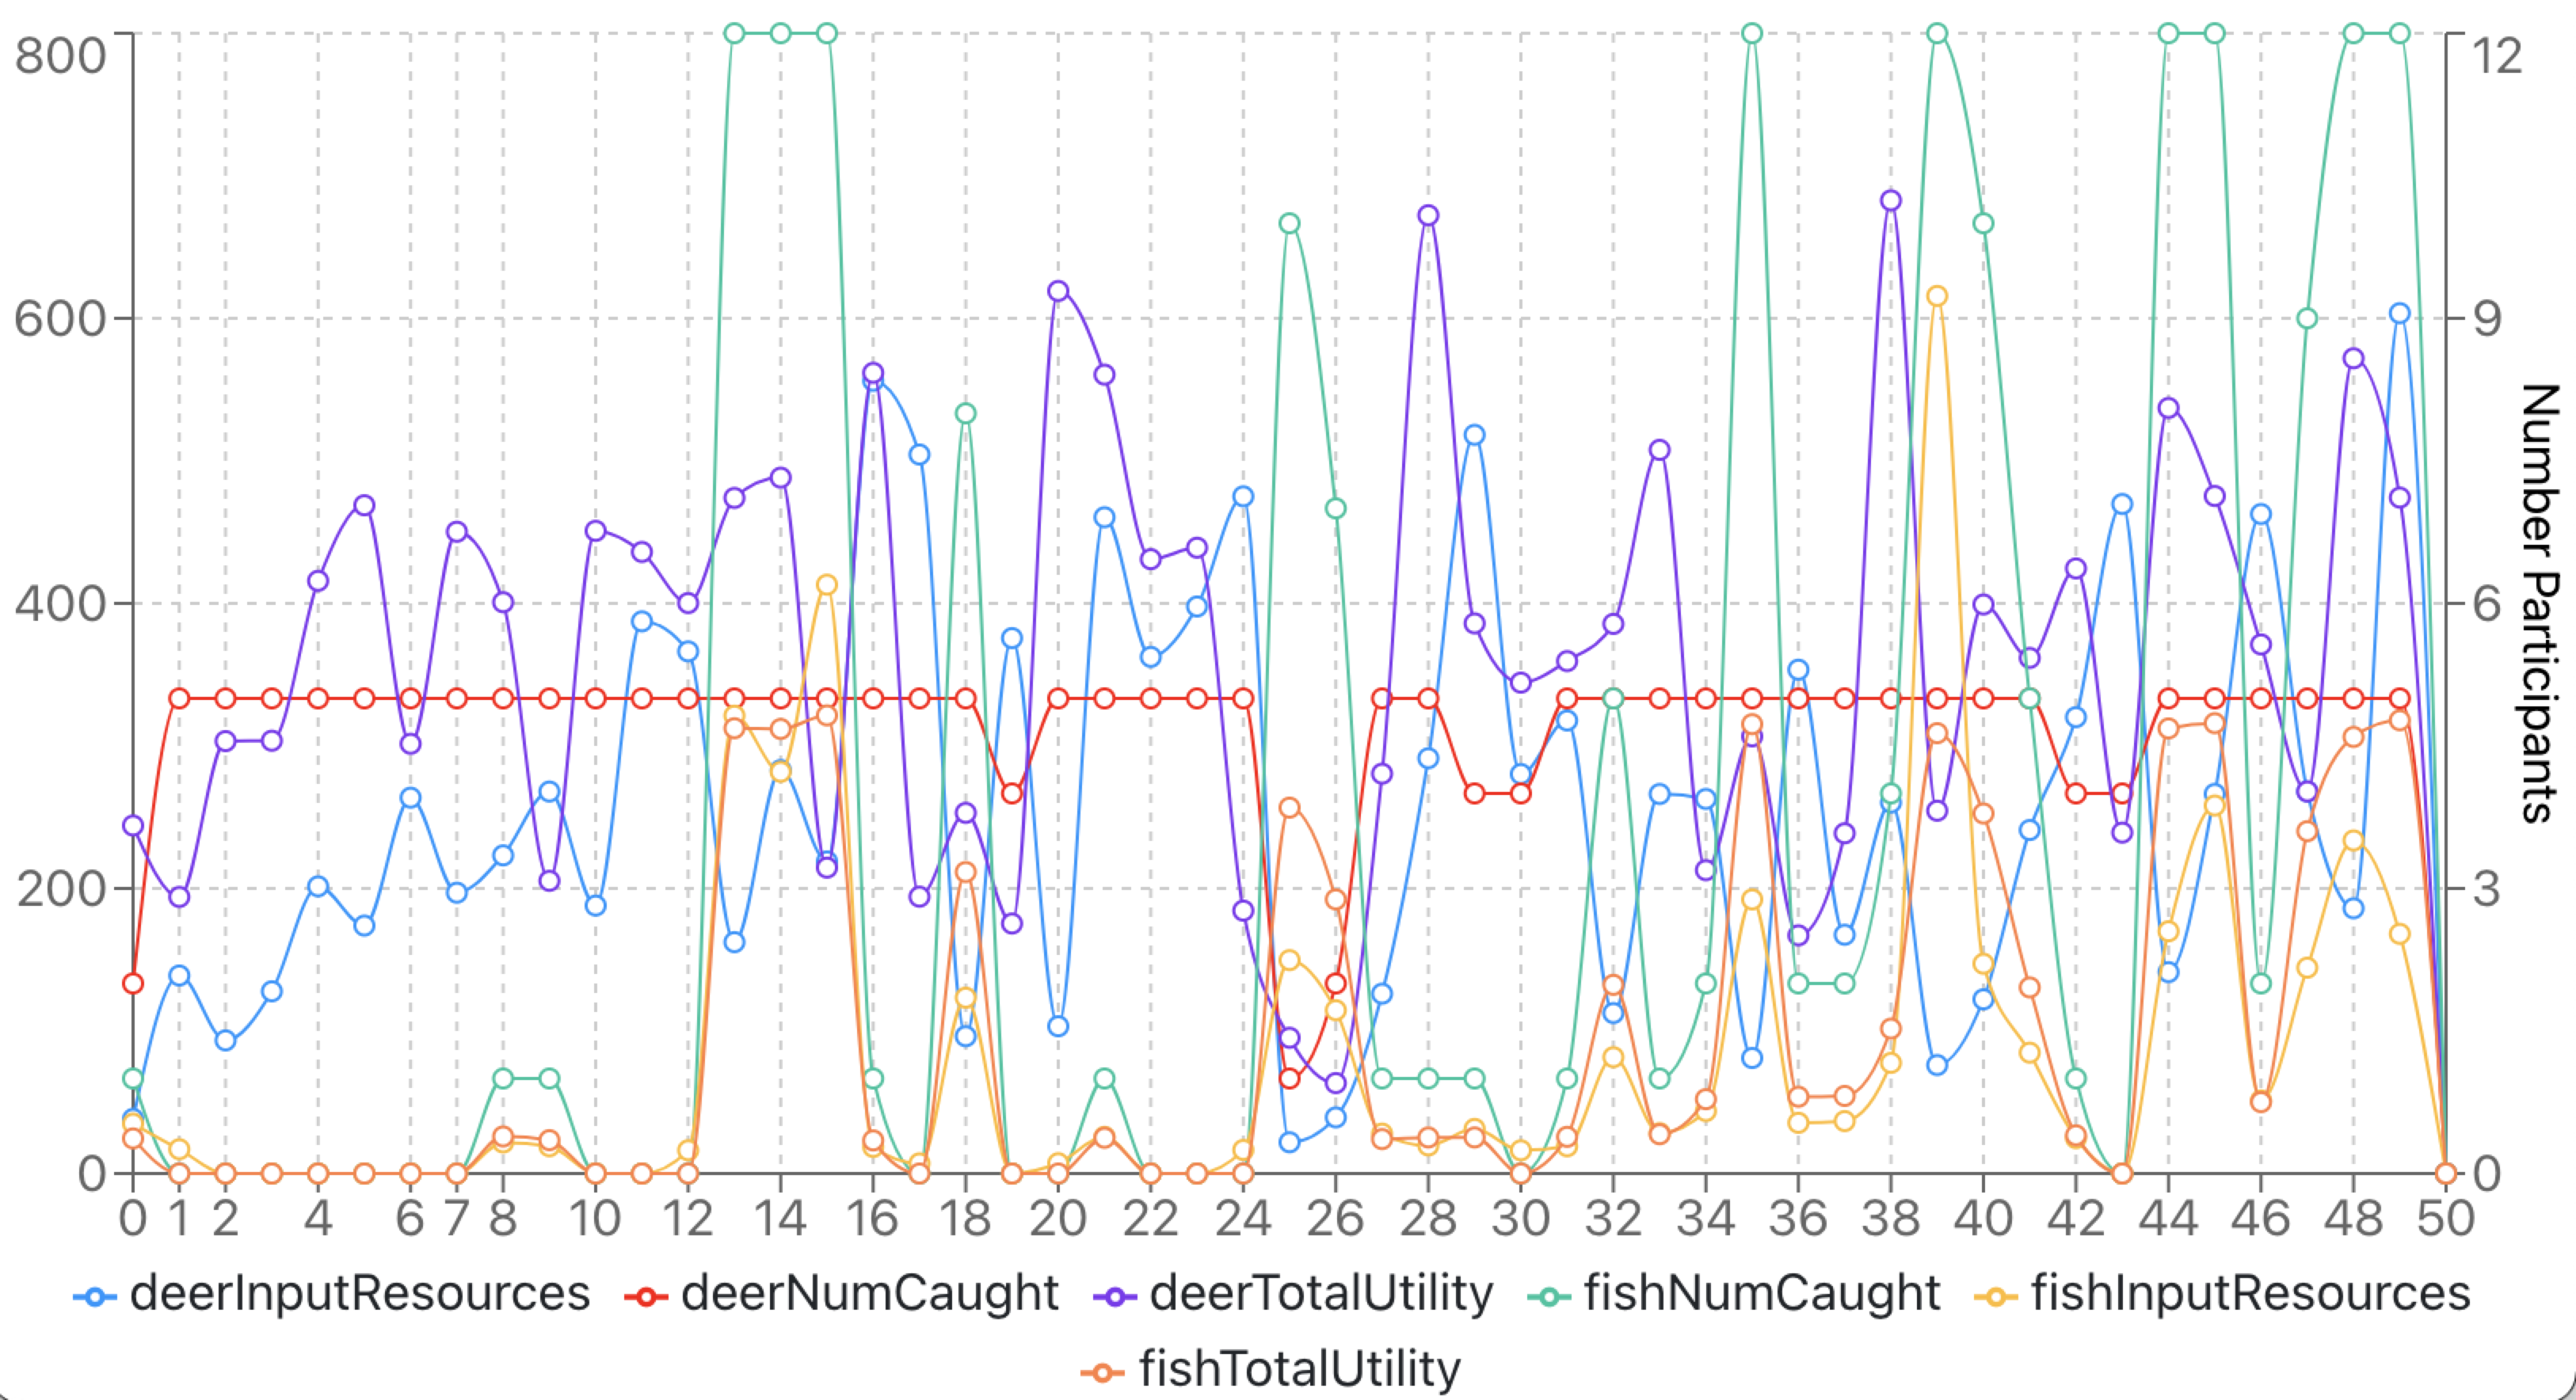
\includegraphics[width=0.8\textwidth]{14_team6_agentdesign/images/foraging.png}
    \caption{Foraging Visualisation}
    \label{fig:foraging}
\end{figure}

\subsection{Distribution of Roles} \label{subsec:Team6_Eval_Roles}

In this simulation result, we could see from Figure~\ref{fig:roles} that our agent is more active in government activities and spends more time managing government departments in the early stage. As time goes by, we are gaining less and less political power and Team 1 becomes the power house instead. This is basically consistent with what we expect to see in design level, because holding government roles could reduce our resources storage due to the cost of actions and will not be always beneficial to us. 

However, our voting strategy will not contribute that much to the election results, which is likely to be influenced by other islands' voting strategies and looks quite different from what we expected to see.
\begin{figure}[H]
    \centering
    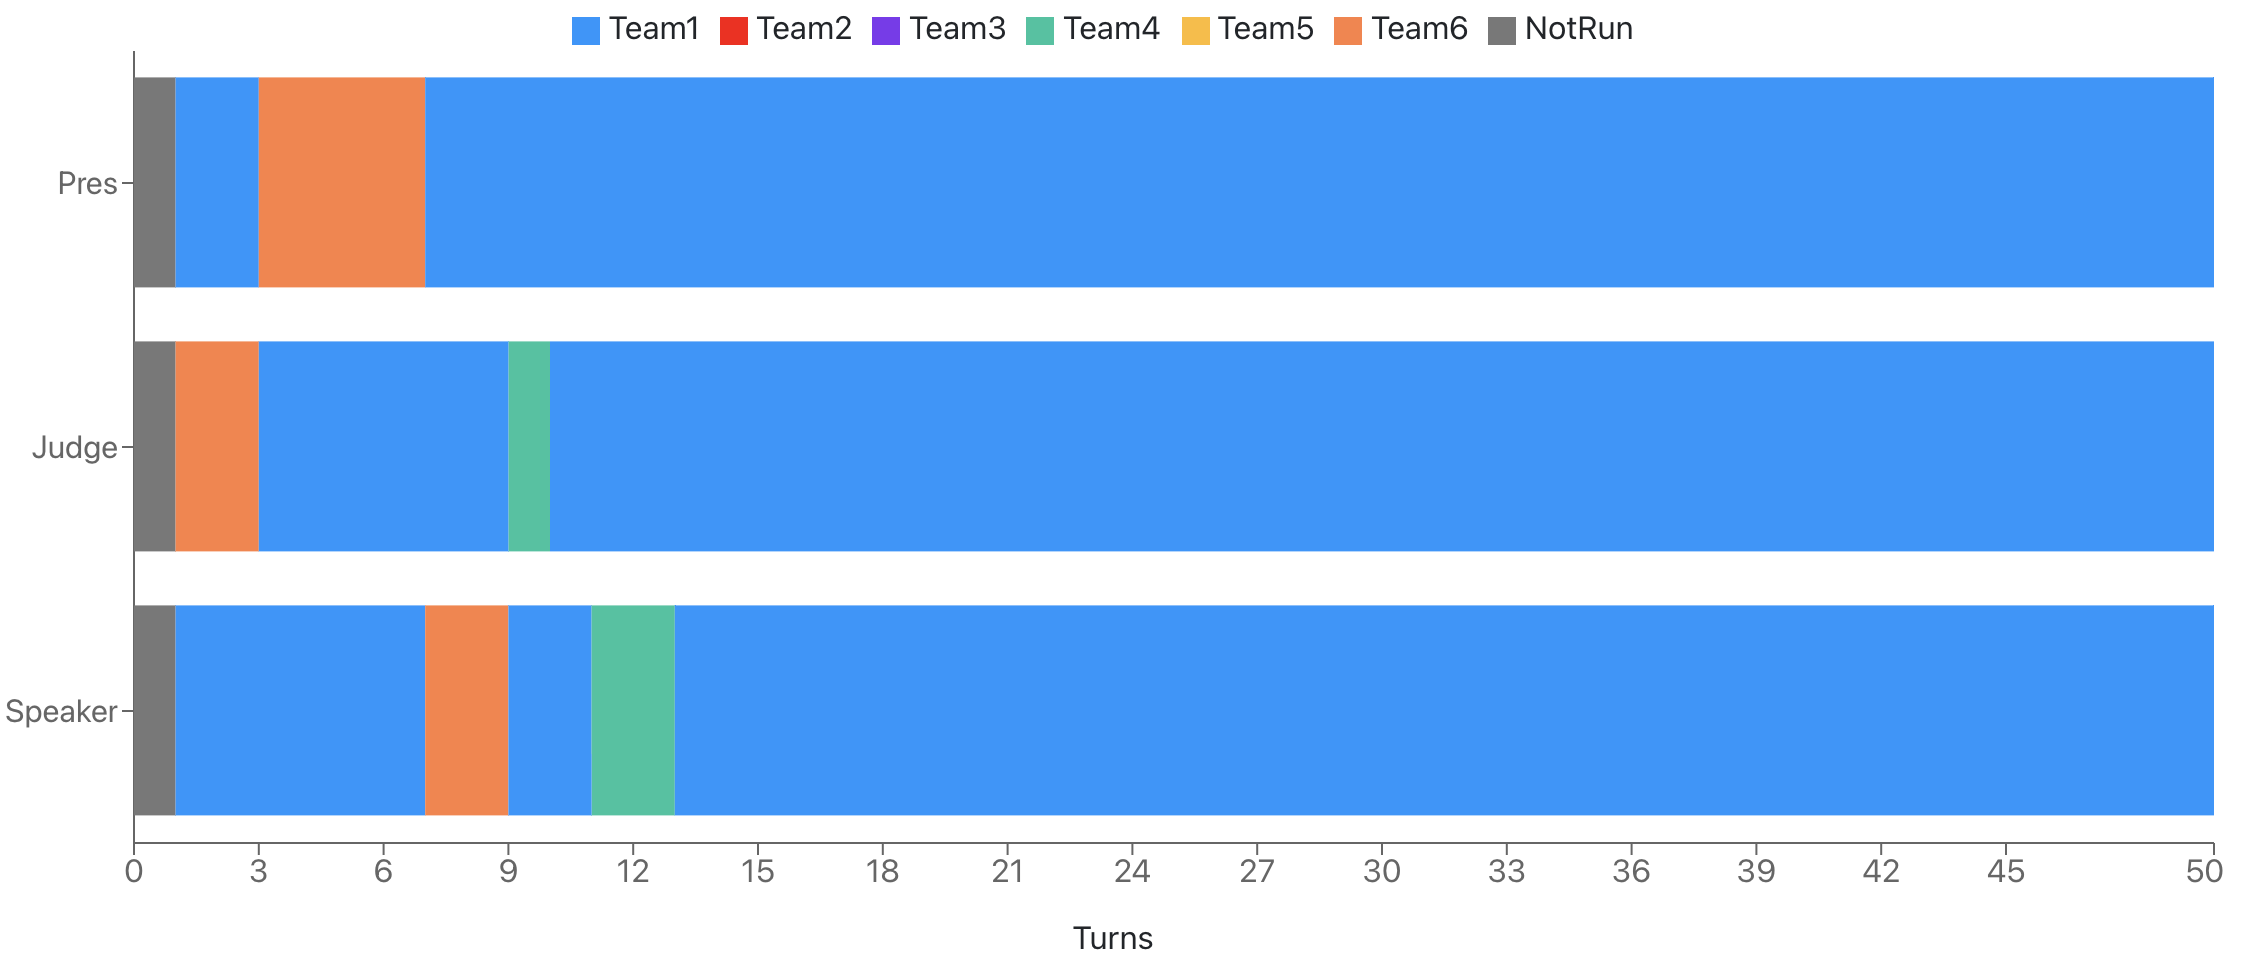
\includegraphics[width=0.8\textwidth]{14_team6_agentdesign/images/roles.png}
    \caption{Distribution of Roles}
    \label{fig:roles}
\end{figure}


\subsection{IIGO Payments} \label{subsec:Team6_Eval_IIGO}

In Figure~\ref{fig:IIGO}, compared to other islands, we manage to run with a lower expected tax level and actually paid more than that. Moreover, we never take more resources than allocated by President and never break the rule, which is also one of our advantages, as we don’t have to waste our resources in sanction payments for breaking rules. By doing this, we reduce the risk of common pool resource exhaustion in a short time, which contributes to the stability and sustainability for the whole system.\\
\begin{figure}[H]
    \centering
    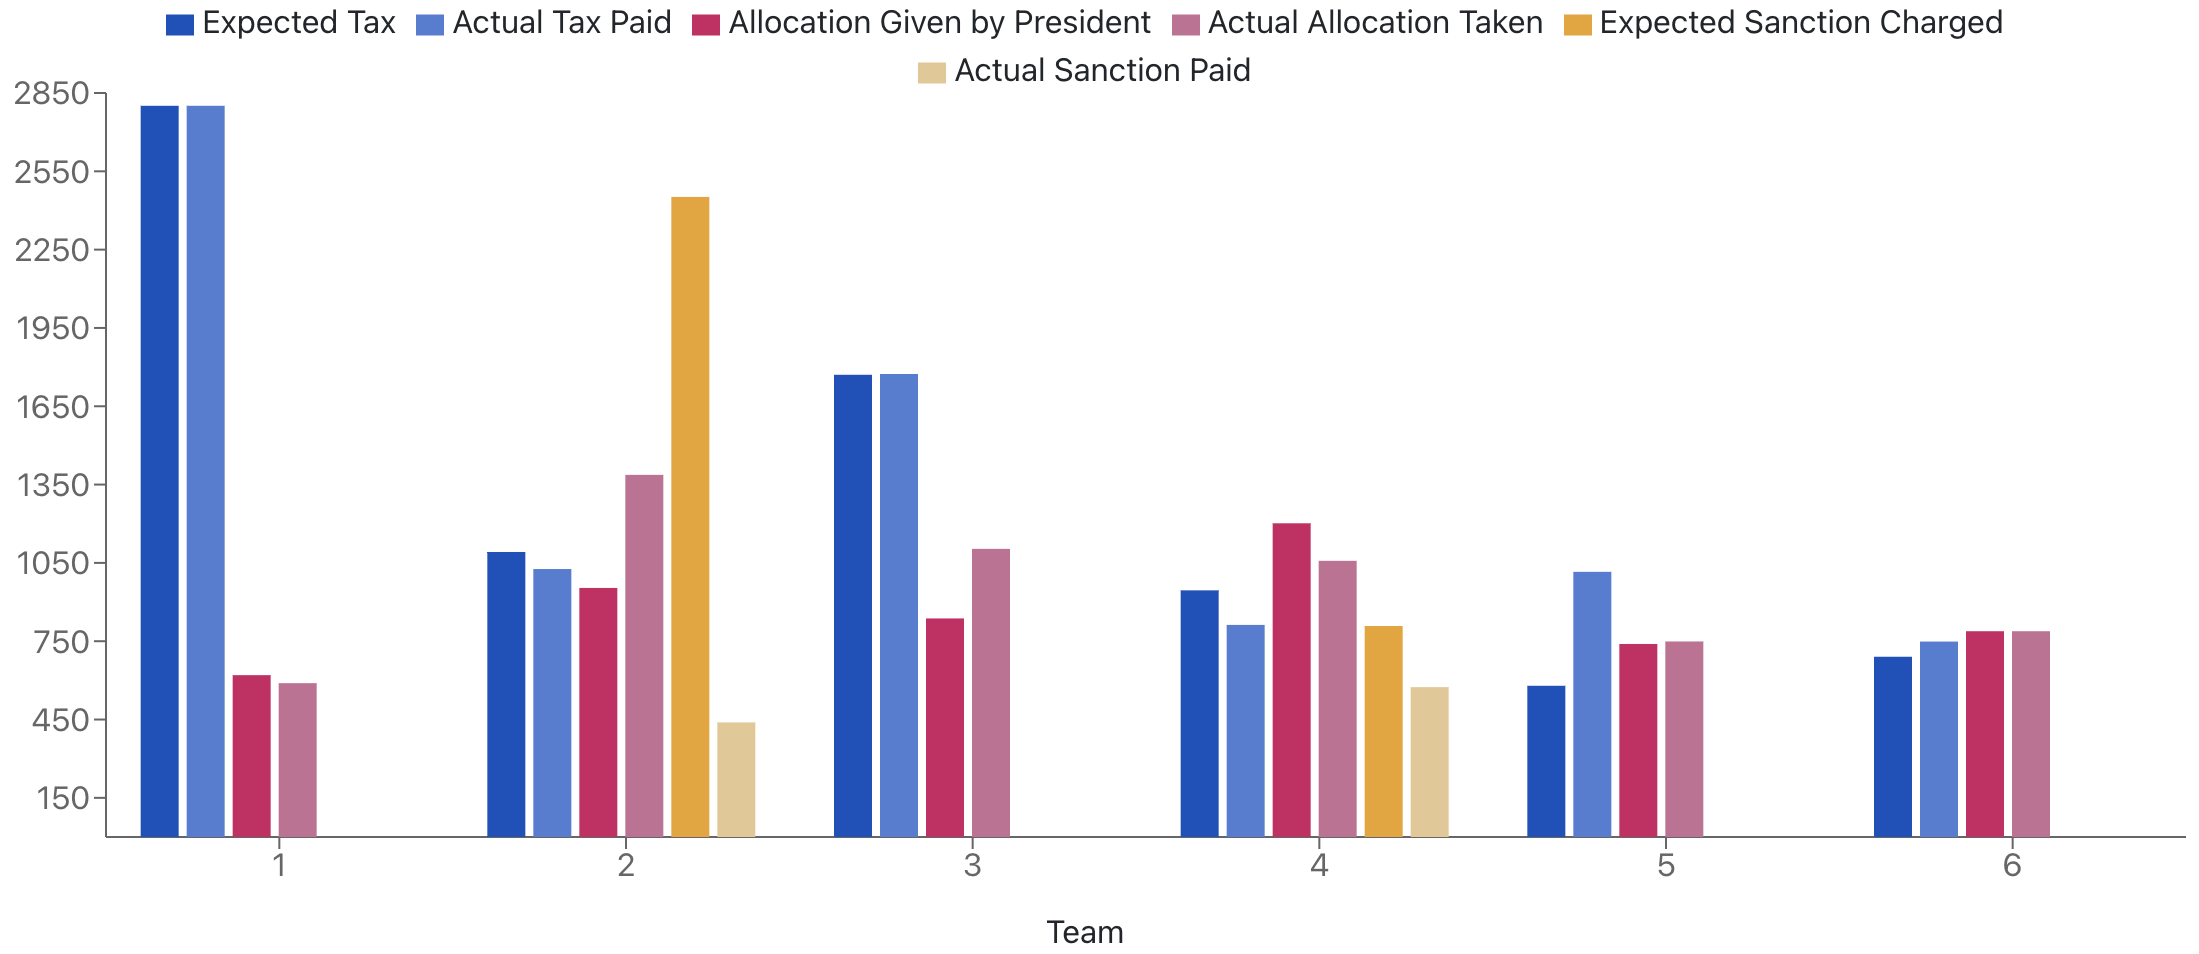
\includegraphics[width=0.8\textwidth]{14_team6_agentdesign/images/IIGO cost.png}
    \caption{IIGO Costs}
    \label{fig:IIGO}
\end{figure}

\subsection{IITO visualisation} \label{subsec:Team6_Eval_IITO}
The following plot shown in Figure~\ref{fig:IITO} visualises the transactions between islands in the IITO sessions. The size of a bubble represents the total magnitude of resources traded by each island. The width of each connecting edge between two islands represents the magnitude of transactions between the two islands. Islands that gave more resources than they receive are indicated by a red border, while islands that received more than they gave are indicated by a green border.

From the plot we could conclude that resources we have received are more than that given by us. Also, our bubble is the penultimate small one, which indicates that we are somewhat inclined to be self-isolated and lack of trade exchanges with other islands. This also could indicate that the friendship with other islands is somewhat not getting along really good based on our own opinion formation towards the other islands.
\begin{figure}[H]
    \centering
    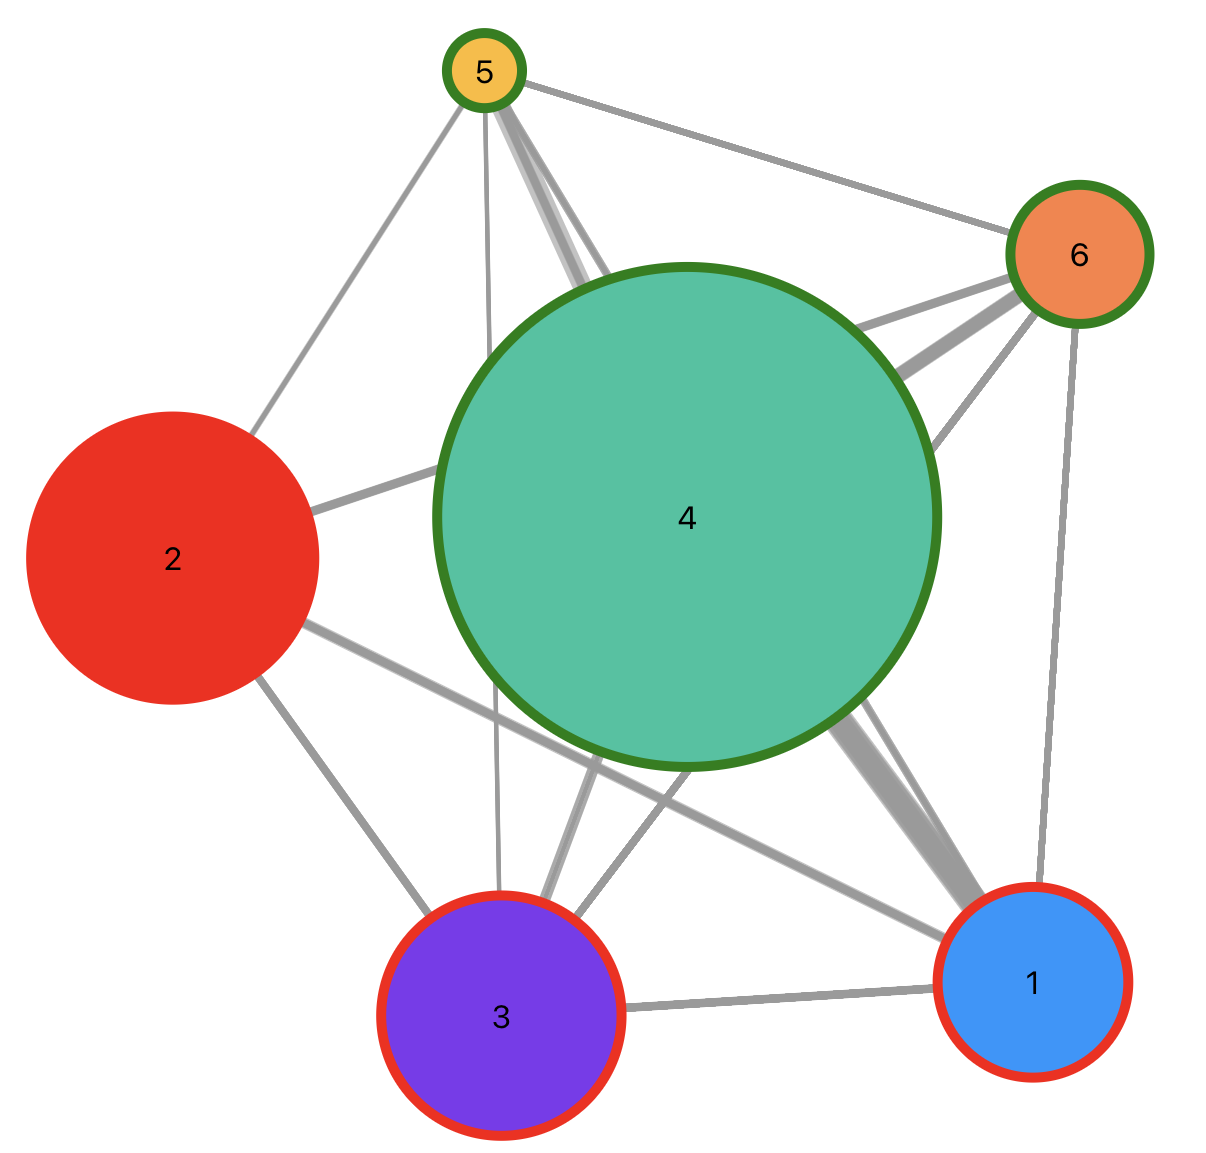
\includegraphics[width=0.4\textwidth, scale=0.1]{14_team6_agentdesign/images/IITO.png}
    \caption{IITO Visualisation}
    \label{fig:IITO}
\end{figure}

\subsection{Resources over time} \label{subsec:Team6_Eval_Resources}

Line charts listed in Figure~\ref{fig:all teams} show the changes about resources on each island and the common pool, as well as the sum of all resources over time. From the simulation results, we could conclude that every island manages to survive long enough, which indicates that our agent adapts well to the operation of the entire system and could automatically take advantage of situations in different specific situations. 

In addition, the resources change curve of our agent as seen in Figure~\ref{fig:team 6} is much smoother than that of some other agents, which shows that we actually have a good grasp of balancing out between income and expenditure of our resources. \\
\begin{figure}[H]
    \centering
    \includegraphics[width=0.8\textwidth]{14_team6_agentdesign/images/resources 1.png}
    \caption{Island 6 Resources Performance against CPR and Total Resources}
    \label{fig:team 6}
\end{figure}
\begin{figure}[H]
    \centering
    \includegraphics[width=0.8\textwidth]{14_team6_agentdesign/images/resources 2.png}
    \caption{Dynamic Resources Level of All Agents from Simulation}
    \label{fig:all teams}
\end{figure}

\section{Future Work} \label{sec:Team6_Future}
Our agent could hopefully be endowed with the ability of machine learning. By using reinforcement learning like Q-learning with CNN, it is possible to let the agent explore the environment by itself while generating the best decision based on what it has learned from the environment. It can become more optimised as the game goes on. However, some limitations became the main issue against the feasibility. To model the environment we need some libraries to build the environment framework. It turns out that programming language we use in this coursework did not supply sufficient machine learning libraries, which becomes a constraint to realise our idea. But we think the potential application of an agent with machine learning ability is feasible to build more robust strategies in dealing with the dilemmas on the overall game.
    \chapter{Simulations}
\section{Introduction}
\label{sec:Simulations:Intro}

The purpose of performing simulations and analysing their results is to explore the efficacy of each agent's strategy under different conditions. We would like to answer questions such as: does the benefit of organisation outweigh the cost? Or, can the agent strategies overcome the foraging dilemma outlined in Section INSERT REF LATER? The analysis encapsulate the purpose of the entire project, and is the final result of all the work we have put in. In this chapter we aim to prove that our platform and the agents are capable of display interesting behaviour and that we can draw conclusions about how behaviors certain behaviours and environmental factors affect a multi-agent system.

\section{Metrics}
\label{sec:Simulations:Metric}

To assist in this analysis we need to draw quantifiable results from the simulations. Thus enters the metrics, these numerical values or visualisation give us information on the events of the game that we can then use to compare numerous simulation and draw insights into what effect the changing of certain parameters has on the game. Some metrics are also worth knowing on a turn by turn basis and as such have been represented as graphs. 


\begin{itemize}
    \item \textbf{Archipelago Survivability}: Turns until all the islands in the archipelago die.
    \item \textbf{First Island Death}: Turns until a single island dies.
    \item \textbf{Island Resources$^1$$^2$}: Resource an island has each turn
    \item \textbf{Gini Index}: A measure of how fair the distribution of resources is across the archipelago.
    \item \textbf{Disasters Survived}: Number of disasters the archipelago has survived.
    \item \textbf{Island Trading$^1$$^2$}: Resources an island has gifted to other islands.
    \item \textbf{Average Disaster Damage Mitigated(ADDM)}: Average disaster damage mitigated by the common pool.
    \item \textbf{Island Foraging Statistics(IFS)$^1$}: Resources an island has invested and gained from foraging.
    \item \textbf{Archipelago Foraging Sustainability(AFS)}: The average forage returns across all islands.
    \item \textbf{IIGO Roles$^2$}: The power each island has at any turn in the game. Power in this case is occupying one of the three roles in IIGO.
    \item \textbf{IIGO Allocations$^1$$^2$}: Amount of resources allocated to each island by the president and the amount the island has taken.
    \item \textbf{IIGO Tax$^1$$^2$}: Amount of resources an island is expected to pay to the common pool for tax and amount the island has paid.
    \item \textbf{IIGO Sanctions$^1$$^2$}: Amount of resources an island is expected to pay to the common pool for sanctions and amount the island has paid.
    
\end{itemize}
\small{$^1$ Presented on a per island basis. $^2$ Presented as a graph}

\section{Baseline Simulation}
\label{sec:Simulations:baseline}

In order to make any meaningful analysis one must first have baseline from which to compare. In our case, this baseline is a 'normal' set of environment conditions which allow the agents to thrive for a significant period of time, around 100 turns. From this baseline we can then start adjusting the configuration of the simulation, either making disaster more frequent/deadly, or making resources more sparse.

Note: If a metric is not of interest to a certain area of exploration it will not be shown.

\subsection{Baseline Numeric Metrics}
\label{subsec:Simulations:baseline:num_metrics}
\begin{table}[htb]
    \centering
    \begin{tabular}{|l|l|}
    \hline
    \textbf{Metric}                     & \textbf{Value} \\ \hline
    \textbf{Archipelago Survivability}  &       \\
    \textbf{First Island Death}         &       \\
    \textbf{Gini Index}                 &       \\
    \textbf{Disasters Survived}         &       \\
    \textbf{ADDM}                       &       \\
    \textbf{AFS}                        &       \\ \hline
\end{tabular}
\caption{Numerical Metrics}
\end{table}

\subsection{Baseline IFS}
\label{subsec:Simulations:baseline:ifs}
\begin{table}[htb]
    \centering
        \begin{tabular}{|l|l|l|l|}
        \hline
        Island            & Investment & Return & Ratio \\ \hline
        \textbf{1: Total} &            &        &       \\
        Deer              &            &        &       \\
        Fish              &            &        &       \\ \hline
        \textbf{2: Total} &            &        &       \\
        Deer              &            &        &       \\
        Fish              &            &        &       \\ \hline
        \textbf{3: Total} &            &        &       \\
        Deer              &            &        &       \\
        Fish              &            &        &       \\ \hline
        \textbf{4: Total} &            &        &       \\
        Deer              &            &        &       \\
        Fish              &            &        &       \\ \hline
        \textbf{5: Total} &            &        &       \\
        Deer              &            &        &       \\
        Fish              &            &        &       \\ \hline
        \textbf{6: Total} &            &        &       \\
        Deer              &            &        &       \\
        Fish              &            &        &       \\ \hline
\end{tabular}
\caption{Island Foraging Statistics}
\end{table}


\subsection{Baseline IIGO Tax, Allocations and Sanctions}
\label{subsec:Simulations:baseline:IIGO}


\subsection{Baseline IIGO Roles}
\label{subsec:Simulations:baseline:IIGO_roles}

\subsection{Baseline Trading}
\label{subsec:Simulations:baseline:trading}
    \chapter{Results}

    \chapter{Evaluation}

    \chapter{Conclusion}


\begin{flushleft}
    \begin{quote}
        ``We are each our own devil, and we make this world our hell.''
        \linebreak
        \emph{Oscar Wilde}
    \end{quote}
\end{flushleft}

Presented here, was the collective effort of 43 humble students united by a fascination with self-governance, Nash equilibria and a willingness to forgo their Christmas break. 

This project successfully produced a simulation of a group of agents with the tools required to collaborate to solve collective action problems. Though limited in intelligence, in certain parameterisations, these agents were able to survive and thrive. This is no mean feat, especially considering that in the early days of this project, a frequently heard phrase was: ``How the fudge are we going to do this?''.

Alongside the success of the simulation, we must also recognise the amazing accomplishment of meta self-organisation. The cohort spanned every timezone, personality, work ethic, haircut, political affiliation and ability to understand sarcasm (pardon the exaggerations here). Yet, despite all that divides us, we were able to come together and produce an impressive piece of work that we are particularly proud of. 

I would like to conclude this report by thanking each and every one of my teammates for their outstanding contributions and unfailing committment to the delivery of this project. I think I speak for all of us when I say that I am amazed at what we have created and it has truly been an experience like no other, but let's not do it again. Please.

    
    % \input{00_example/example.tex}
    % \input{01_introduction/introduction.tex}
    % \documentclass[a4paper, twoside]{report}
% Template author: Y. Panagis

\usepackage[english]{babel}
\usepackage[utf8x]{inputenc}
\usepackage[T1]{fontenc}
\usepackage{listings}
\usepackage{hyperref}
\hypersetup{colorlinks=false}
\usepackage{lscape}
\usepackage{subfigure}
\usepackage{amsmath}
\usepackage{graphicx}
\usepackage[colorinlistoftodos]{todonotes}
\usepackage[ruled, vlined]{algorithm2e}
\usepackage{verbatim}
\usepackage{float}
\usepackage{tikz}
%\usepackage{algpseudocode}
\usepackage{tabularx}
%\usepackage{multirow}
\def\checkmark{\tikz\fill[scale=0.4](0,.35) -- (.25,0) -- (1,.7) -- (.25,.15) -- cycle;}


\usepackage{amsthm}
\usepackage{amsfonts}
\newtheorem{definition}{Definition}
\newtheorem{rule_IIGO}{Rule}


%% Sets page size and margins
\usepackage[a4paper,top=3cm,bottom=2cm,left=3cm,right=3cm,marginparwidth=2cm]{geometry}

\begin{document}
    % The Title, Author Name, Date, and abstract go here
    \title{Self-Organising Multi-Agent Systems: MVP Specifications}
    \author{SOMAS Class 2020-2021}
    \date{\today}
    \maketitle

    \tableofcontents    
    % if you are adding a new chapter, create a new folder in the root directory of the project
    % it should begin with a two digit number, followed by an underscore and the name of the section.
    % This keeps the order of the sections in the side view in keeping with the order of the document.
    
    \chapter{Introduction}

\begin{flushleft}
\begin{quote}
    "Therein is the tragedy. Each man is locked into a system that compels him to increase his herd without limit – in a world that is limited. Ruin is the destination toward which all men rush, each pursuing his own best interest in a society that believes in the freedom of the commons."
    \linebreak
    \emph{Ellinor Ostrom}
\end{quote}
\end{flushleft}

In the current political climate, while shaking a fist angrily at the television screen, one often finds oneself asking the question, 'Are human beings even capable of creating institutions for the common good?'. As such, it is worth investigating whether electronic multi-agent systems are able to do a better than mere mortals, in the eventual hope of designing stronger, fairer socio-technical systems.

This project explores the ability of independent agents to self-organise in order to solve long and short-term collective risk dilemmas. The collective risk dilemma poses a challenge to a group of agents whereby they must balance their own interests against the interests of the collective. 

The objective of this project was to design and implement two collective risk dilemmas as well as a system of agents capable of mitigating the risk. In order to do this successfully, the system contains adequate communication and self organisation tools for the agents to make use of.

The specific problem posed can be summarised as follows: islands in an archipelago are incentivised to pool their resources in order to collectively survive environmental disasters but must balance this against an interest in their own survival and properity. The method of resource replenishment is deer hunting and fishing. The populations of these resources are limited and neither of these foraging methods have guaranteed returns. 

The self-organisation tools available to the islands are:

\begin{itemize}
    \item Inter-Island Trade Organisation: a forum for trading gifts with other islands.
    \item Inter-Island Forecasting Organisation: a forum for sharing disaster predictions.
    \item Inter-Island Government Organisation: a forum for self-governance.
\end{itemize}

    \chapter{Roles and Responsibilities}


Team 2 Ezgi Ozyilkan test PR
Team 4 Rudolfs Spuris - test PR
Team 6 Yiqiang Huang test PR

    \chapter{Specification}
    \chapter{Game Design}

\section{Design Approach}

A game was designed to meet the requirements outlined by the specification to provide structure to the inter-island interactions and decisions. This \emph{game design framework} provides a basis for the simulations, experiments and evaluations into different agent strategies and system designs.

The game is structured as series of \emph{seasons} and \emph{turns}, which concludes once all of the islands die. The objective for the islands is to survive for as many turns and seasons as possible. The following definitions provide a detailed outline of the relevant terminology used to formalise the game definition and description.


\begin{definition} \label{def:gamestart}
    \textbf{Game start} is defined as the beginning of a simulation. Each simulation can be configured using a number of parameters, including but not limited to the cost of living, probability of a disaster and initial resources in the common pool.
\end{definition}

\begin{definition} \label{def:turn}
    A \textbf{turn} is defined as a series of exchanges between agents in which islands receive resource updates, attend Inter-Island Organisation meetings (e.g. IIGO, IIFO, IITO), and interact with one another and the game state through \textbf{actions}. A turn can be broken down as follows:
    \begin{enumerate}
        \item Resource Updates for each island and on global game state.
        \item The Inter-Island Governmental Organisation (IIGO) decides rule changes, elections, sanctions.
        \item The Inter-Island Forecasting Organisation (IIFO) provides a forum for information exchange to mitigate both short and long term risk dilemmas.
        \item Inter-Island Trade Organisation (IITO) facilitates gift exchanges and allows agents to communicate to make deals between one another without organisation supervision.
        \item Islands submit decisions on their actions to the server to formally end the turn.
        \item Check if a disaster occurs this turn.
        \item Server processes actions and updates game and island states.
            \begin{itemize}
                \item A cost of living is subtracted from an islands pool before the next term. This is the simulation-level equivalent to using resources to stay alive (e.g. food consumed). These resources are permanently consumed and do NOT go into the common pool. Note: this is NOT the same as the tax.
                \item Check if the game is over.
                \item Check if any islands are \textbf{critical} (i.e. below the threshold).
                \item Check if any islands are \textbf{dead}.
            \end{itemize}
    \end{enumerate}        
\end{definition}

\begin{definition} \label{def:gameseason}
    A \textbf{season} is defined as a series of turns and concludes with a disaster. Seasons formalise the flow of the game and provide a method to track the number of disasters the islands survive.
\end{definition}

\begin{definition} \label{def:gamestate}
    The \textbf{game state} is the set of information an island receives at the start of each turn. This includes, but is not limited to, the resources it was allocated the previous turn, the geographical location of the islands, the quantity of resources left in the common pool and the set of rules for the turn (including any rules that were modified the previous turn). It is important to note that each island's game state is private. Therefore, no other island can see another island's resource allocation.
\end{definition}

\begin{definition} \label{def:gameaction}
    An \textbf{action} is a decision an island can make or that is made by any Inter-Island Organisation that updates the game state. Actions can be made at different stages within a turn both within Inter-Island Organisations and at the end of a turn. This includes but is not limited to taking resources from or donating resources to from the common pool, rule changes in the IIGO, and gift requests or acceptances. The following is a brief overview of the actions that agents can take:

    \begin{itemize}
        \item \textbf{Foraging}: Agents can decide to allocate resources to generate resources through foraging
        \item \textbf{Gifting}: Agents can choose to send, and accept resource gifts from other agents through the IITO
        \item Agents can take resources from and give resources to the Common Pool
        \item Agents can execute \textbf{role actions}. These actions relate to actions agents can take in organisations such as the IIGO and are explained in further detail in the following chapters.
        \item Agents can share information through the IIFO, for example, regarding predictions of future disaster locations, magnitudes and timing.
    \end{itemize}
\end{definition}

\begin{definition} \label{def:gameseason}
    The \textbf{common pool} is a pool of resources shared by the islands. It is used to mitigate disasters, and act as a central resource storage for tax payments, and agents to share and take resources through self organisation.
\end{definition}

\begin{definition} \label{def:critical}
    A \textbf{critical} island is defined as an island whose resources are below the minimum threshold. When this occurs, an island is allowed a grace period during which it is expected to request gifts from other islands in order to reach the minimum amount of resources required to stay in the game.
\end{definition}

\begin{definition} \label{def:death}
    A \textbf{death} occurs when an island was in a \textbf{critical} state for $N$ turns. The exact number of turns affects the difficulty of the game so it was investigated and is discussed in simulations and results section. Once an island is dead, it can no longer participate in the simulation.
\end{definition}

\begin{definition} \label{def:gameover}
    \textbf{Game over} is defined as the end of the simulation and occurs when all islands have died or the simulation is completed - whichever occurs first.
\end{definition}

Figure~\ref{fig:gamedesign-flow} depicts a high level diagram of the general flow and structure of the game.

\begin{figure}[!htb]
    \centering
    \includegraphics{03_gamedesign/images/gamespec-flow.png}
    \caption{High Level Game Specification Flow Diagram}
    \label{fig:gamedesign-flow}
\end{figure}

\subsection{Design Choice Justification}
Every action taken in the game adds to the dilemma placed on the agent to explore how they interact and attempt to overcome challenges through self-organisation. To complicate matters further, the meetings occur only to form agreements, which can also be broken after they are made. The allocation also occurs first to assist islands that are struggling by allowing them to take from the common pool immediately and use these resources to forage or, at a minimum, pay their tax.

\subsection{Game Parameters}
Many of the parameters within the game can be modified to adjust the difficulty of the game. It should be noted that some of these parameters have a greater impact than others. For example, the agents may or may not have access to the common pool threshold level and this knowledge, or lack thereof, will result in entirely different agent performance. This because each agent relies on different strategies and approaches each aspect of the game in a different way. For example, while some agents rely more on social strategies and cooperation to mitigate unknown risk, others rely heavily on calculations and predictions. Each agent strategy will come with its own unique set of benefits and limitations in the context of the game, performing better or worse, under different conditions.

% Start of section on implementation

\section{Implementation}
\label{sec:GD:implementation}

Implementation design was important as the majority of the class were involved in writing simulation code. As such, dedicated \emph{infrastructure} engineers from each team were elected to form an infrastructure team responsible for building the central part of the game, otherwise known as the \emph{server}. Each team's infrastructure engineer was tasked to own the implementation of a slice of the server.

One such sub-team was the \textbf{core} infrastructure team, responsible for building the core parts of the game server. Inputs were taken from the entire class to choose the best implementation strategies and design--a solid and simple core foundation was paramount to allow clean continuous integration of code and ideas from all contributors. The subsections below detail implementation specifics of the game's simulation.

\subsection{Architecture}
\label{sec:GD:implementation:arch}

The structure of the game was closely modelled after a \emph{client-server} model\footnote{\url{https://en.wikipedia.org/wiki/Client-server_model}}, but note ``closely''--whilst the nomenclature was taken directly from the aforementioned model, there are some differences. \emph{Server} and \emph{client} in this context bear the following definitions:

\begin{definition} \label{def:server}
    The \textbf{server} is the central game runner, responsible for initiating game events (such as a disaster or the start of a turn). Certain events require the actions of agents, in which the server will invoke a function on the agents to receive a response. Further, the server acts as a source-of-truth for the game's state.
\end{definition}


\begin{definition} \label{def:client}
    Each \textbf{client} is implemented by an agent. The client provides an interface of functions in which the server can invoke. Moreover, clients may also invoke certain functions from the server's interface to read specific game information.
\end{definition}

The major difference of this architecture to a traditional client-server model is that, in the former, the stateful central server drives the other clients (by triggering events and eliciting responses), as opposed to clients sending stateless requests to a server to receive a response in the latter. Furthermore, whilst the client and server have been separated architecturally, the entire system still operates as a single process.

\subsection{Technology Stack}
\label{sec:GD:implementation:techstack}

Agreeing on a technology stack proved to be challenging--the class had varying levels of programming expertise. Whilst Prolog\footnote{\url{https://en.wikipedia.org/wiki/Prolog}} and Qu-Prolog\footnote{\url{https://staff.itee.uq.edu.au/pjr/HomePages/QuPrologHome.html}} (an extension to the former) were used to cover topics in the lectures, the class did not favour them over more well-known and established imperative programming languages. Hence, time was dedicated to formulate a consensus to decide on the technology stack, with primary focus given on the choice of implementation language. Firstly, high priority requirements were defined for the stack:

\begin{itemize}
    \item Easy to learn
    \item Easy to setup
    \item Cross-platform
    \item Easily maintainable
    \item Friendly features
\end{itemize}

Minimum Working Examples (MWEs) comprising a single server and two clients were created in different stacks, which served as starting points for discussion among members of the class. The MWEs implemented are as follows.

\begin{enumerate}
    \item \textbf{Multi-language}\footnote{\url{https://github.com/SOMAS2020/somas-demo}}.
          A multi-language (C++ server with a Python and a C++ client) MWE was first set up. It was first thought that allowing agent teams to choose the programming language they were most familiar with would speed up development. However, despite this stack's benefits, it could not be easily made cross-platform. Each agent's code would need to be run in a separate process, and Inter-Process Communication (IPC) would be required to pass messages. IPC is quite low-level and varies vastly among different systems. Further, protocols for the IPC would also need to be set up to pass the correct message, and having no strong typing as in a strongly-typed language (or session-typed\footnote{\url{https://arxiv.org/abs/1906.03836}}) approach would make it difficult to maintain and develop.

    \item \textbf{Python}\footnote{\url{https://github.com/SOMAS2020/somas-demo-py}}.
          Python\footnote{\url{https://www.python.org/}} is widely used by the scientific community in recent years with the growing ubiquity of scientific computation packages available for it. As such, Python was a strong contender as most of the class already know Python from past projects. However, Python's weak typing meant it scored low on the ``easily maintainable'' part--the server and client interfaces would benefit a lot from strong typing. While add-on static typing tools such as \texttt{mypy}\footnote{\url{https://mypy.readthedocs.io/}} could be employed (it is also used in the MWE), it would still not be as powerful as built-in strong typing as in languages such as C\# and Go.

    \item \textbf{C\#}\footnote{\url{https://github.com/SOMAS2020/somas-demo-cs}}.
          C\#\footnote{\url{https://docs.microsoft.com/en-us/dotnet/csharp/}} is the flagship language of the .NET ecosystem. C\# shares a large part of its design to the more popular C++. C\# is strongly-typed, and promotes use of clean Object-Oriented Programming (OOP). Many of the features from C/C++ that can be \emph{dangerous} are not present or hidden, making it more beginner friendly. A drawback is that some experience with C-family languages is required to pick up C\# quickly.

    \item \textbf{Go}\footnote{\url{https://github.com/SOMAS2020/somas-demo-go}}.
          While most of the class was not familiar with Go\footnote{\url{https://golang.org/}}, its simple language syntax and highly-featured toolchain make it very easy to learn. The modern Go toolchain makes it extremely simple for programs to work cross-platform. While Go's omission of OOP and generics might be seen as a disadvantage, it makes it an easy language to learn, and prevents pitfalls commonly caused by such ``features''. Go, like C\#, is strongly typed. Moreover, Golang's great support for WebAssembly\footnote{\url{https://webassembly.org/}} would prove useful for visualisations, further detailed in~\ref{sec:GD:implementation:visualisations}. Another nice feature is that concurrency can be easily implemented in Go, which meant that agent actions could be run concurrently to speed up simulations.
\end{enumerate}

After discussion, scores (out of 10) were given for each stack. Table~\ref{table:techstackscores} shows these scores. The multi-language and Python approaches were removed from consideration--the former due to its low total score and the latter because of its low maintainability. The decision between C\# and Go was harder, and ultimately resulted in a \emph{simple majority} vote by the class. 37 people voted in total, with 25 in favour of Go. Hence, Go was finally chosen.

\begin{table}[h]
    \centering
    \caption{Scores given for each stack based on requirements}
    \label{table:techstackscores}
    \begin{tabular}{|c|c|c|c|c|c|c|}
        \hline
        Stack                     &
        \makecell{Easy              \\ to \\ learn}              &
        \makecell{Easy              \\ to \\ setup}              &
        \makecell{Cross-platform} &
        \makecell{Easily            \\ maintainable}             &
        \makecell{Friendly          \\ features}                 &
        \makecell{Final             \\ score \\ (out of 50)}
        \\
        \hline
        Multi-language            &
        6                         &
        2                         &
        0                         &
        2                         &
        10                        &
        20
        \\
        \hline
        Python                    &
        8                         &
        6                         &
        8                         &
        3                         &
        8                         &
        34
        \\
        \hline
        C\#                       &
        6                         &
        5                         &
        8                         &
        9                         &
        8                         &
        37
        \\
        \hline
        Go                        &
        8                         &
        8                         &
        10                        &
        8                         &
        6                         &
        40
        \\
        \hline
    \end{tabular}
\end{table}


\subsection{Visualisations}
\label{sec:GD:implementation:visualisations}

\subsubsection{Toolchain}
A benefit from the choice of the Go technology stack was that it supports compiling source code into WebAssembly out of the box. WebAssembly can be run efficiently in most modern browsers, which meant that in-browser simulations can be run and then visualised on a website.

The website (\url{https://somas2020.github.io/SOMAS2020/}) features... % TODO:- Vis team: yp717 et al.

\subsection{Engineering Practices}
\label{sec:GD:implementation:practices}

Developing and maintaining a codebase with contributions from around 40 developers was projected to be non-trivial. Therefore, good software engineering practices and rules were employed to be upheld by all contributors to make the process smoother and--where possible--automated.

\subsubsection{Code testing}

While Go is strongly typed and would mean that most errors can be detected at compile-time (or even at time of coding with its performant language server), having unit and integration tests greatly improved the maintainability and ease of development of the project--these issues were particularly important as this was a large-scale group software engineering project--developers stepping on each other's toes is a common occurrence in non-tested group project code. Henceforth, tests were required for non-trivial server-side code.

<<<<<<< HEAD
\subsection{Peer Review}

Peer review was also setup via GitHub pull requests--each change required the approval of another member in the infrastructure team. This practice not only promoted consistent code design and implementation, it minimised mistakes and ensured that the code implementation meets design and implementation requirements set forth. Further, as there was variation in programming skill among code contributors, knowledge sharing was facilitated by code reviews. This was also a critical opportunity for engineers to learn more about the other code being contributed to the project.

\subsection{Continuous Integration}
\label{sec:GD:implementation:practices:CI}

Via GitHub Actions\footnote{https://github.com/features/actions}, continuous integration was set up. Each Pull Request (PR) was set up to trigger automated runs of written tests and a full simulation in addition to static code analysers such as linters. These checks must all pass for the PR to be merged into the main branch. Automated testing and code analysis saved time and facilitates regression testing, as all tests--existing and new--were run for each change. Running a full simulation also served as a good stress-test for the system to make sure that it does not crash on a similar full simulation. Further, automated tests were run on a reference system (Ubuntu 20.04 with Go 1.15.5 and Node 14), helping to prevent system-specific quirks or bugs from polluting the codebase.

\subsection{Continuous Development}

On receiving PR approval, passing automated tests and finally merging into the main codebase, the visualisation website is automatically rebuilt with the latest changes. This saved time as manual builds were not required. The builds were produced on a reference system (identical to that mentioned in~\ref{sec:GD:implementation:practices}), ensuring consistent builds free from system-specific quirks. Further, automated builds meant that the website always runs on the latest codebase.
=======
\subsubsection{Peer Review}

Peer review was also setup via GitHub pull requests--each change required the approval of another member in the infrastructure team. This practice not only promoted consistent code design and implementation, it minimised mistakes and ensured that the code implementation meets design and implementation requirements set forth. Further, as there was variation in programming skill among code contributors, knowledge sharing was facilitated by code reviews. This was also a critical opportunity for engineers to learn more about the other code being contributed to the project.

\subsubsection{Continuous Integration}

Via GitHub Actions\footnote{https://github.com/features/actions}, continuous integration was set up. Each Pull Request (PR) was set up to trigger automated runs of written tests and a full simulation in addition to static code analysers such as linters. These checks must all pass for the PR to be frequently merged into the main branch. Automated testing and code analysis saved time and facilitates regression testing, as all tests--existing and new--were run for each change. Running a full simulation also served as a good stress-test for the system to make sure that it does not crash on a similar full simulation. Further, automated tests were run on a reference system (Ubuntu 20.04 with Go 1.15.5 and Node 14), helping to prevent system-specific quirks or bugs from polluting the codebase.

\subsubsection{Continuous Deployment}

On receiving PR approval, passing automated tests and finally merging into the main codebase, the visualisation website is automatically rebuilt with the latest changes. This saved time as manual builds were not required. The builds were produced on a reference system (identical to that mentioned in the Continuous Integration section), ensuring consistent builds free from system-specific quirks. Further, automated builds meant that the website always runs on the latest codebase.
>>>>>>> 962869f9957a17b0764e8a570c39fa55a16b5576

    \chapter{Environment}
\section{Foraging}

\begin{definition} \label{def:Welfare}
\textbf{Welfare} is the state of wealth, it can either be personal or collaborative (social).
\end{definition}

\begin{definition} \label{def:Maximising Social Welfare}
\textbf{Maximising Social Welfare} is a strategy which attempts to maximise the total amount of welfare (resources) the islands have.
\end{definition}


\subsection{Foraging Background}

Foraging is a fundamental requirement that is needed as it is a method of obtaining more resources from the starting amount. Foraging is based on the concept of inputting resources to get a return.

\subsubsection{Underlying Concept}

The primary objective of foraging in this game is to introduce a dilemma to the agents in order to investigate their behaviours and whether they work together despite different personal goals. Including two methods of foraging promotes decision making among the islands, allowing for strategic interactions to maximise personal benefits while still reaching the overarching goal of survival. 

The inspiration for our concept of foraging comes from the stag hunt game. Thus, it introduces elements from it. Specifically, this approach results in a game with \textbf{no dominant strategy} and in which \textbf{an agent's choice can impact another agent's}.

The process of stag hunt is that each agent selects a method of hunting without the information of the other agents. The social welfare (total payoff) is significantly reduced if their choices differ. The selection of stag suggests that the agent is going for higher \textbf{payoffs} whilst the selection of hare indicates that the agent is \textbf{risk aversion} as both agents are required to stag hunt to get any personal welfare (see Definition~\ref{def:Welfare}).

\subsubsection{Modifications to the Original concepts} 
A few changes have to be made to make this dilemma viable for our multi-agent system, in addition to adding realism. 

\begin{enumerate}
    \item The dependency was changed to be based on the input resources rather than the number of islands participating. This added a more realistic element to the dilemma as in reality a hunt’s return would be based on the amount of resources (different possible resources: people, food, water and materials) entered rather than the number of islands participating.
    \item Instead of a specified return, probabilistic return was implemented which adds a randomness element to the game to prevent pattern recognition. These probabilities can be tied to the population, disasters, forecasting and number of animals hunted.  
\end{enumerate}

Furthermore, the dynamics of our agents and allowing for a more complex decision-making interaction between islands and the environment have been explored. It is worth mentioning that some of these design ideas were implemented in the coursework. These changes have been made to make foraging more volatile and unpredictable, adding to the complexity of the system, allowing the teams to further evaluate the agents’ performance on observing and to use learned knowledge to take action.

\subsubsection{Tier System}

The deer hunting and fishing is divided into tiers, which depend on the total amount of input resources. Tiers represent the number of fish that can be caught in a given day, and the “zero” tier represents the cost associated with getting to the hunting location. Beyond the zero tier, the cost of catching another deer or fish will decrease as it is easier to catch the second animal than the first one, since the agents have already arrived at the hunting location. Therefore, if the agents do not even enough to reach the first tier, then they wouldn't get any returns. It should be noted there is a limit to how many animals the agents can catch in a given day.

The focus of fishing is to avoid risk at the expense of payoff. This means that all tier requirements are lower than those for the deers. However, the return is also lower thus if only one island goes fishing they are still expected to have a low return as long as they have enough resources to catch the first fish. Thus, the benefit of deer hunting is higher payoffs. However, these improved returns come at the cost of significantly higher tier thresholds. Therefore, it is possible for a single island to go deer hunting without enough resources to reach the hunting location leading to no return.

\begin{equation}
\text{Increments of catching $n$ animals}=
\left( \begin{array}{ll@{}}
n=0 \longrightarrow \Delta^0 = 1 \\
n=1 \longrightarrow \Delta^1 = 0.8^1 \\
n=2 \longrightarrow \Delta^2 = 0.8^2 = 0.64 \\
n=2 \longrightarrow \Delta^3 = 0.8^3 = 0.512 \\
n=4 \longrightarrow \Delta^4 = 0.8^4 = 0.4096\\
\end{array} \right) 
\label{eq:Cumulative Cost 1}
\end{equation}

\begin{equation}
\text{Utility Tier Cost}=\ \sum_{n=0}^{n} \Delta^{n} = \Delta^{0} + \Delta^{1} + \Delta^{2} + \Delta^{3} + \Delta^{4} + ....
\label{eq:Cumulative Cost 2}
\end{equation}

Equation~\eqref{eq:Cumulative Cost 1} and Equation~\eqref{eq:Cumulative Cost 2} show the formulation of the decay function for tier system. The tier system is shown in the Figure~\ref{fig:Foraging Tier System} where $n$ stands for the tiers, with decay costs ($\Delta$) of $0.8$ for the deer hunt and $0.6$ for fishing.

\begin{figure}[!htb]
    \centering
    \includegraphics[width=0.9\textwidth]{04_environment/images/Foraging Tier System.PNG}
    \caption{Foraging Tier System}
    \label{fig:Foraging Tier System}
\end{figure}

The amount of resources inputted is scaled using a variable and the tiers are then calculated with them, the higher the tiers the lower the cost to catch the next animal. However, the total cost increases up to a daily catch limit. This means that if teams collaborate, they can invest less as individuals to get a collectively greater return through deer hunting. If they invest too much, then they will over spend as they reach the daily catch limit. As a result, it is more beneficial for some teams to go fishing because it has a higher daily catch limit, although it comes with lower returns. In other words, there is a need for some self-sacrifice to reach the maximum welfare (see Definition~\ref{def:Welfare}). Moreover, fishing is a similar foraging method with the key difference being that it utilised a normal distribution and the start of the tiers.

\subsection{Example Distribution}
\subsubsection{Example of the Distribution for Foraging Return (Deer Hunting - Payoff Dominant)}

\begin{figure}[!htb]
    \centering
    \includegraphics[width=1\textwidth]{04_environment/images/Distribution of Foraging returns Deer Hunting.PNG}
    \caption{Deer hunting payoff dominant Distribution for foraging return}
    \label{fig:Distribution of Foraging returns Deer Hunting}
\end{figure}

To increase the risk of deer hunting, a Bernoulli Random Variable ($D$) was used to prevent guaranteed resource returns after a hunt. While the Exponential Decay ($W$) is to disincentive too much resources being placed in hunting and hoping for a high return. However, this all comes with the benefit of significantly higher ($2\times$) returns than fishing.

Figure~\ref{fig:Distribution of Foraging returns Deer Hunting} represents the return utility which will be multiplied by an output scale to give the return payoff. The Figure~\ref{fig:Distribution of Foraging returns Deer Hunting} shows the average \textbf{expected mean} return utility, in colour, after $1000$ iterations which is close to the \textbf{real mean}.

\newpage
\subsubsection{Fish hunting - Risk Aversion}

Fishing is similar to Deer hunting, except that it uses only a Normal Distribution ($F$), which focuses on avoiding risk by being very predictable and safe. Figure~\ref{fig:Distribution of Foraging returns Fishing} illustrates the return utility for fishing.

\begin{figure}[!htb]
    \centering
    \includegraphics[width=1\textwidth]{04_environment/images/Distribution of Foraging returns Fishing.PNG}
    \caption{Fishing Risk aversion Distribution for foraging return}
    \label{fig:Distribution of Foraging returns Fishing}
\end{figure}

As seen in Figure~\ref{fig:Distribution of Foraging returns Deer Hunting}and Figure~\ref{fig:Distribution of Foraging returns Fishing}, the return for the deer is almost double that of the fish return whilst the fish return is much easier to obtain due to the lower cost of catching fish.

\newpage
\subsection{Solution Concepts}
\subsubsection{Dominant Strategy}

In this implementation, there is no dominant strategy. Therefore, if an agent decides to go deer hunting, whereas all the other islands are fishing, that agent would not get the best return possible. Hence it is not the best strategy. Whilst if an agent goes fishing and there are a sufficient amount of agents deer hunting, then that agent would be passing on the opportunity of to gain a larger return in deer hunting. Hence, it is not the best strategy either.

\subsubsection{Nash Equilibrium}

In the regular stag hunt game, there are two pure Nash Equilibria, where both agents go for either payoff or risk aversion. In our implementation, there are multiple Nash Equilibria. These are the points where the islands cannot benefit themselves by moving to deers hunting to generate more return. As there is a limit to how many deers that can be hunted thus by moving to deer hunting they are getting a worse return than if they just stayed at fishing. Whilst the islands at the deer hunt are already making a greater return and have no reason to switch to fishing.

\subsubsection{Pareto Optimal Strategy}

At some point, all agents will be in a position where changing foraging methods will not yield any better income for themselves and in fact also hinder others. This is due to the max daily deer hunt limit which creates a maxim return on the deer hunt. Therefore there will be points where the islands will change as the amount of resources being entered into both methods of foraging is the most efficient, this being where deer returns are maximised. There may also be a point where the agent can benefit by switching away from deer hunting. However, this will cause the other islands in the deer hunt to have a worse pay off due to a possible drop in tier resulting in worse returns.

\begin{figure}[!htb]
    \centering
    \includegraphics[width=0.7\textwidth]{04_environment/images/Pareto Optimal Strategy.PNG}
    \caption{Pareto Optimal Strategy}
    \label{fig:Pareto Optimal Strategy}
\end{figure}

\subsubsection{Social Welfare Maximisation}

It is possible for these islands to find the social welfare maximum (see Definition~\ref{def:Maximising Social Welfare}) in this foraging function with enough time. The islands could identify the exact amount of resources needed, for both fishing and deer hunting, to achieve the best return according to the maximum number of animals. Thus, by cooperating who goes where and spends how much, they are able to maximize their returns without spending more resources than necessary.

\subsubsection{Population Density}

Introducing a model that controls the population density of deer allows us to increase the complexity of the foraging function. In short, the deer hunting capacity decreases with decreasing population and increases with an increasing population. This then influences the maximum deer per hunt parameter ($n$), which in turn results in a more complex return calculation function (\texttt{\textbf{DtotalReturn}}), which would make it harder for agents to figure out forage tier boundaries to optimise their strategies.

The population change can be dynamic depending on various environmental factors, fetched from the rest of the system. For example, a disaster could supposedly cause the population density of deer to halve, making it harder to forage and therefore, causing lower returns. In this current implementation, a single species population model and more specifically logistic modelling for the deer and fish population was implemented. 
The model is described in Equation~\eqref{eq:Population Density}.

\begin{equation}
\frac{\mathrm{d} P}{\mathrm{~d} t}=k(N-P)
\label{eq:Population Density}
\end{equation}

\begin{itemize}
    \item $P$ is the total population. 
    \item $N$ is the maximum deer population (carrying capacity\footnote{The maximum population size of a biological species that can be sustained in a specific environment.}).
    \item $k$ is the growth coefficient.
    \item $t$ is time.
\end{itemize}

In Figure~\ref{fig:Deer population over time}, the simulation of the implemented logistic model can be observed, with a growth coefficient of $0.2$ and $N$ of $8$. It can be seen that there is an unpredictable pattern to population changes, which would be interesting to see affecting the tier system and in extend, the deer and fish foraging strategies of the agents.

\begin{figure}[!htb]
    \centering
    \includegraphics[width=1\textwidth]{04_environment/images/Deer population over time.PNG}
    \caption{Deer population over time (turns) under Logistic modelling with a growth coefficient of 0.2.}
    \label{fig:Deer population over time}
\end{figure}

Furthermore, In our implementation, $k$ and $N$ are constants. 

Modelling the population (or linking it to other environmental elements) allows us to make sure that the system’s dynamics are varying, making it harder for islands to settle onto a single foraging method because it always results in better returns. Pareto optimality is therefore harder to achieve and thus maximising social welfare (see Definition~\ref{def:Maximising Social Welfare}) is trickier, requiring agents to make more informed decisions, recognizing possible patterns. Of course, that would be an easier task for the islands, if they had knowledge on what is affecting the population (i.e. disasters), whereas a logistic model function might be more abstract in the eyes of our agents, requiring more processing. 

\subsubsection{Method of Resource Allocation}

Moreover, there is a parameter to allow either an equal split of returns after foraging regardless of the input, or a proportional split dependent on the amount of resources inputted by each island. Both of these implementations work in accordance to the previous specification. Such change allows us to observe the concept of free-riding further, looking at how greedy islands behave in the case of uniform resource returns.

The distribution method is based on two scalars. The first scales the inputs to the tiers, allowing the agent to choose how much they wish the tiers to cost. After which, the number of fish or deer caught is chosen by the tiers which goes into their respective distributions. The output of these distributions are then multiplied by the output scale. This allows the user to adjust the return amount each island can obtain, the output scalar should be above the cost of living in order to ensure the islands have enough resources to survive.  

\subsection{Future Work}

Further work could be done to make sure that there is enough complexity to explore the dynamics of our agents. Due to the project’s time constraints, some interesting ideas were not implemented but were thoroughly examined during the design process.

An important add-on to our previous implementation could be the enforcement of laws by the IIGO for the number of islands that can go foraging. That would introduce the need of internal agent relationships, adding another level of decision-making complexity to the agents. The specific alteration could result in some interesting findings. For example, there could be an auction scenario where islands would bid with their input resources, where only the highest bidders would be able to forage, as limited by the IIGO. Therefore, the islands with the lowest resources would be out-bidded, possibly causing a long-term resource depletion that would need to be mitigated by the more resourceful islands later in the game. It would be interesting to see how such change would affect the free-rider problem and how islands would adjust their strategies to out-bid other islands.

Another change that could be made is to let islands choose who they want to forage with. The islands would communicate with each other in form of direct messaging or voting to reach a decision. 
Essentially, our speculation is that agents would avoid the free-riding problem in both cases by enabling agents to make collective decisions based on communicated resource contributions. That’s because free-riders would be out-voted or not invited for foraging. That, in combination with the aforementioned tier system, would possibly result in all the islands contributing as much as possible to the input foraging “pool”. However, it would be interesting to see if islands can then reach Pareto optimality, where every single agent gets the best possible return for their input.

In addition to the above suggestions, agents would be restricted to just a single foraging area where they would only be allowed to forage with one neighbouring island using a ranking algorithm. This could alter the game's dynamics as an agent would only have limited partners (i.e. other islands) to forage with i.e. other islands in the same limited area. The aforementioned islands could be explicitly decided or randomly allocated. This could also be enforced and implemented as future work. Moreover, this particular scenario could be extended by programming prey densities to be geo-focused, where prey populations could vary between regions on the “map”. Islands would then need to make a strategic plan on how their ranking of neighbouring islands would change in accordance to their returns and returns broadcasted from other island pairs.

As discussed earlier, the population density of deer is a parameter that allows us to increase the complexity of the foraging function, tying it up to a realistic population model. It would be interesting to see what would happen if the growth coefficient increases, causing a population growth and observing the islands’ dynamics. Will they keep on “investing” higher resources each turn, taking advantage of the deer and fish abundance, or will they stick to their original, safe and static strategy?

In addition, going into resource allocation, the utility is in fact multiplied by an output multiplier. Therefore, the user determines the output multiplier value, as well as the resource allocation. Thus, agents can receive either a proportional split or an equal allocation of resources based on the users' decisions. Moreover, a few questions that be could be asked about the islands relationship and behaviour are: Will the islands seek to minimise inputs and benefit from the more generous islands, even at the cost of being allocated a lower tier? Will they input just enough to maximise the tier they are foraging in? Or, will they observe other island’s previous contributions and make a decision based on that?

Finally, more foraging options could be added in future implementations. For example, a third foraging technique; whale hunting could be created. This option would have an even higher return than deer hunting, deeming it an appealing forage method. The barriers of entry could be similar to that of the deer hunting method in this scenario but at the same time, there would be a more spaced out/expensive tier system. This combination would potentially incentivise cooperation between islands, if their strategy was to maximise returns. Also, as additional foraging methods have been introduced, the type of return was fixed for each foraging method and observe how agents decide to behave. For example, the deer and fish hunting methods result in returns proportional to inputs, whereas the whale hunting method would result in an equal split of returns between all participating islands. Would this mean that islands choose a fairer division of returns and not go on whale foraging at all? Or would they be intrigued by the higher costs and choose whale hunting over the other foraging methods? In the latter question agents would need to take into account that an island may enter an insignificant amount of resources and reap a large return. It is therefore up to the islands to decide if the higher payoff is worth the risk of other islands free-riding.

All the aforementioned behaviours are, of course, influenced by the island tactics. Therefore, an island programmed to be greedy could not cease to be greedy, no matter how the surrounding islands’ behaviours change, unless the greedy island can adapt. Therefore, agent strategies must attempt to draw conclusions on specific foraging methods and modify their strategies where appropriate.

\newpage
\section{Disaster}
\subsection{Disaster Background}

A game was designed, where agents directly confront a disaster and its risks once every round. This subset of the game creates a dilemma, where each island (agent) has to survive. They will have the opportunity to work together by investing collectively to the common pool, the disaster will be mitigated if the islands invest enough resources to reach a desired threshold. Otherwise, the islands would face negative impact, which would diminish their available resources. It is worth mentioning that the disaster will first extract resources from the common pool, and then if not enough resources have been invested, resources will be depleted from each island proportionally to their island’s damage.

Furthermore, the disaster was designed to comprise of an epicentre (eye of the storm), which is limited within the archipelago bounds, it is represented using Cartesian coordinates (EpiX, EpiY). Therefore, all islands or a subset of islands may be affected due to their proximity to the disaster epicentre. The island’s proximity to the disaster epicentre is directly proportional to the island’s damage. In other words, the island's available resources will be diminished based on the disaster magnitude and its location with respect to each island’s fixed location.

The following example can briefly explain the dilemma:

The closest an island from the eye of the storm, the larger the severity on that island. Therefore, the more resources are depleted. Let’s say the disaster epicentre hits around Island 1 as shown in Figure~\ref{fig:Disaster eye of the storm severity} and that the desired common pool threshold has not been met. Island 1 would be experiencing severe damages , and Island 2 and 6 some damages and the other islands low to no damage. Therefore, Island 1, 2 and 6 have the risk of not surviving if they are lacking resources, whereas Island 3, 4, and 5 would not be affected as much by the disaster.

\begin{figure}[!htb]
    \centering
    \includegraphics[width=1\textwidth]{04_environment/images/Disaster eye of the storm severity.PNG}
    \caption{Disaster Epicenter effects}
    \label{fig:Disaster eye of the storm severity}
\end{figure}

\newpage
\subsection{Future work}

There are multiple future work ideas that would be developed in the design aspect such as; a deterministic disaster which would be  designed as a straight line that accumulates during the days, once the threshold was met then the disaster would occur. Another deterministic disaster idea would be to link the disaster’s magnitude to time. Thus, agents would have to learn from past disaster occurrences, creating a memory. Agents would start learning from past disasters and would be able to forecast the next one. Therefore, the agents would be able to forecast that if a disaster did not surface for a long period of time, then the magnitude of the next disaster will be much larger than the previous one.

Another idea is that agents can invest into forecasting. Therefore, agents will have access to a history of past disasters, which would be utilised to learn and gain knowledge in order to predict the upcoming disasters.

Thus, the more resources invested by the agents in forecasting, the more disaster history data will be provided. This would enable the agents, to apply machine learning techniques to such data, allowing them to acquire more accurate and precise predictions of future events and develop better risk assessments. Therefore, agents will acquire knowledge, when investing in any of their resources.


\section{Common Pool}
\subsection{Common Pool Background}

A game was designed where one group of six islands (agents) have access to a common-pool resource. In micro-level, each island intends to maximise its utility while in macro-level, all the islands want to maintain sustainability and be protected by the upcoming disaster. The above description specifies a collective action problem where n-agents (six in our case) are seeking access to a common pool resource that is sufficient to satisfy some agents but not to satisfy all of them.

A Linear Public Goods (LPG) Game was implemented, where all the agents individually own some resources and try to maintain and increase them, by foraging, but also contribute a part of them to the common pool. This common pool is used for the payment of expenses of the institutional roles and for the protection towards the disaster.

In more detail, the common pool is represented by a structure with following characteristics:

\begin{itemize}
    \item Common Pool Threshold.
    \item Amount of Resources.
\end{itemize}

According to the specifications of a Linear Public Goods Game, the agents should be able to perform the following actions:  

\begin{itemize}
    \item Request Resource from the Common Pool.
    \item Contribute Resource to the Common Pool. 
\end{itemize}

And the Common Pool is responsible for two more actions: 

\begin{itemize}
    \item Mitigate disaster.
    \item Deplete islands after a disaster.
\end{itemize}

The common pool threshold is a fixed value and known to islands and its resources will be given to each island based on the severity of the damages.

If the amount of resources in the common pool exceeds the total effect of disaster, then the leftover amount of resources in the common pool will be used for the next round.

Since the goal of each island is to maximise its utility, the following dilemma shows up: islands can free ride by not contributing to the common pool and yet receiving the benefits after a disaster or if they are aware that they would not be depleted by the disaster - since they are far away from the eye of the storm - they might also not contribute to the common pool and thus the rest of the islands would be severely destroyed.

The following example can briefly explain this dilemma:

If the epicentre of disaster is known to the islands and happens to coincide with the location of Island 1, then Island 4 might not contribute at all to the Common Pool since it will not be affected by the disaster. Moreover, Islands 3 and 5 that will not be severely hit might contribute a small amount to the Common Pool or even zero amount (free riding case). Since the rest of the islands might contribute to the Common Pool, then Islands 3 and 5 will be profited by the contribution of others.

importance of prevention and incentivise islands to contribute to the Common Pool is highlighted, thus if the amount of resources in the common pool exceeds the threshold when the disaster happens, then the “power” of disaster towards the islands and common pool will be decreased. It makes sense in real life, as more preparation will result in less damage. The actual damage of disaster is decreased by half.

\subsection{Example Distribution}
This can be described by the examples in Table~\ref{tab:Demonstration of how the common pool work in different scenarios}, which shows 4 possible scenario:

\begin{itemize}
    \item Contribution to common pool does not meet threshold and common pool cannot fully mitigate disaster’s damage.
    \item Contribution to common pool does not meet threshold but common pool can fully mitigate disaster’s damage.
    \item Contribution to common pool meets threshold but common pool cannot fully mitigate disaster’s damage.
    \item Contribution to common pool meets threshold and common pool can fully mitigate disaster’s damage.
\end{itemize}

\begin{table}[!htb]
\begin{center}
\begin{tabular}{|l|c|c|c|c|}
\hline
                               & \textbf{Scenario 1} & \textbf{Scenario 2} & \textbf{Scenario 3} & \textbf{Scenario 4} \\ \hline
\textbf{Disaster Total Damage} & 1000                & 200                 & 1200                & 1200                \\ \hline
\textbf{CP's Threshold}        & 500                 & 500                 & 500                 & 500                 \\ \hline
\textbf{CP's Current Value}    & 300                 & 300                 & 500                 & 700                 \\ \hline
\textbf{CP's Multiplier}       & 1                   & 1                   & 0.5                 & 0.5                 \\ \hline
\textbf{Mitigated Damage}      & 300                 & 200                 & 500                 & 1200                \\ \hline
\textbf{Remaining Damage}      & 700                 & 0                   & 100                 & 0                   \\ \hline
\textbf{CP's Remaining Value}  & 0                   & 100                 & 0                   & 100                 \\ \hline
\end{tabular}
\end{center}
\caption{Demonstration of how the common pool work in different scenarios}
\label{tab:Demonstration of how the common pool work in different scenarios}
\end{table}

In scenario 1, the disaster total damage is high. However, there is no preparation from the islands through contribution to the common pool. As a result, the common pool could not mitigate all of the damage and $70\%$ of the damage will be directly on the islands.

In scenario 2, even though there is no preparation, the common pool is still able to mitigate all of the damage thanks to the low damage of disaster. The leftover resource in the common pool will stay there.

In scenario 3, the disaster damage is high. Fortunately, the islands have prepared themselves moderately through contribution to the common pool. Thus, the islands only have to take very little leftover damage.

In scenario 4, the disaster damage is high, and the islands have prepared themselves very well. As a result, the damage is fully mitigated by the common pool, and there is still leftover resource in the pool. 


\subsection{Future Work}

To observe behaviors of agents in different settings, the future work on the common pool could be centered around varying the values of different parameters such as threshold and threshold multiplier. The forecasting function of the disaster part can be used as a tool to variate the common pool’s threshold and multiplier accordingly. In events that damage could be high, the preparation should be done more carefully, thus the common pool’s threshold can be raised to let islands know about potential damage from disaster. The same thing can be done for threshold multiplier, where the multiplier will be greater for bigger disaster. Since threshold and multiplier both encourage the preparation for disaster, one of them can be fixed at certain seasons to observe different behavior of agents when it comes to varying different parameters. 

It is worth mentioning that the functionality of making the threshold unknown to the islands would be implemented in our future work.
    \chapter{Inter-Island Governmental Organisation (IIGO)}


The role of IIGO is to maintain, update, and revise the rules concerning provision to managing the long-term collective risk dilemma (ltCRD). 

\begin{itemize}
    \item There will be 3 distinct branches in the IIGO: the \textbf{legislative branch}, \textbf{executive branch} and \textbf{judicial branch}\footnote{This is, as no surprise, inspired by the separation of powers in Western democracies.}.
    \item Each role is put in power according to the  transfer-of-power rules (see Section~\ref{subsec:transfer-of-power} for more detail).
    \item The head of the legislative branch is the Speaker, the head of the executive branch is the President, and the head of judicial branch is the Judge.
    \begin{itemize}
        \item  The Speaker, President and Judge are selected, through a democratic election, from the islands in the archipelago\footnote{This naming is inspired by the roles in the US Government.}.
        \item The resources gathered by the archipelago are endogenous, hence acting on the institutional powers granted to the Speaker, President or Judge costs resources. 
        \item For their duty, the President, the Speaker and the Judge receive a salary for each of their turns in office (see Section~\ref{subsec:salary} for more detail).
        \item The limit of the powers of the President, Speaker and Judge are defined in this chapter (e.g. the Speaker can only call one vote per turn).
 
    \end{itemize}
\end{itemize}

\subsection{IIGO Specific Definitions}
\begin{definition} \label{def:ballot}
    A \textbf{ballot} is related to each island's \textbf{power} to support or disagree with the rule specified in the vote called by the President and to vote in favour or against an island for a specific role (i.e. the President, Speaker, Judge) at each round of the game.
\end{definition}


%\begin{definition} \label{def:vote}
    %A \textbf{vote} is related to a role's (i.e. the President, Speaker, Judge) \textbf{power} to call a vote for a specific rule or an election.
%\end{definition}


\begin{definition} \label{def:tax}
    The \textbf{taxation} is related to the President's \textbf{power} to request a specific \underline{\textbf{minimum}} amount of contribution from each island to the common pool at each round of the game. 
\end{definition}

\begin{definition} \label{def:alloc_req}
    An \textbf{allocation request} is related to each island's \textbf{power} to request a specific amount of resource allocation from the President at each round of the game.
\end{definition}


\begin{definition} \label{def:rule_prop_list}
A \textbf{rule proposal list} is related to each island's \textbf{power} to propose a specific rule to be passed to the President at each round of the game.
\end{definition}

\begin{definition} \label{def:invst}
    An \textbf{investigation} is related to the Judge's \textbf{power} to acquire information to make a decision, followed by a calculation of the expected results and checking whether some specific rules have been obeyed, exclusively for the actions carried out by the \textbf{islands}. 
\end{definition}


An example of an \emph{investigation}: The President has permitted the island $X$ to take the amount of $Y$ resources from the common pool. Upon \emph{investigation} carried out by the Judge, it is revealed that the amount of resources taken out from the common pool by the island $X$ is, in fact, $Y'$ such that $Y' \neq Y$.


\begin{definition}
\textbf{Monitoring} is a government official's \textbf{power} to perform event recognition and to check whether some specific rules have been obeyed.
\end{definition}

An example of \emph{monitoring}: The Speaker has performed only the following action: \emph{counted the votes and calculated the result} for a rule. Upon \emph{monitoring} carried out by the President, it is noticed that the Speaker has not made any \emph{announcement}. Hence, the Speaker has not followed their obligation to \emph{announce} the result of any vote held.

See Section~\ref{sec:accountability} for more information about which roles can monitor which ones.


\begin{definition}
\textbf{Investigative-monitoring} is a government official's \textbf{power} to acquire the information used in acting on a governmental power followed by calculation of the expected results and checking whether some specific rules have been obeyed, exclusively for the actions carried out by a government official they are responsible for.
\end{definition}

An example of \emph{investigative-monitoring}: The Speaker has performed the following actions: \emph{counted the votes and calculated the result $R$} for a vote $V$ and \emph{announced} the result $R'$ for the vote $V$. Upon \emph{investigative-monitoring} carried out by the President, it is noticed that $R' \neq R$. Hence, the Speaker has modified the announced result.


\begin{definition}
The \textbf{sanction} is related to the Judge's \emph{power} to punish non-compliant islands when their disobedience is confirmed through investigations at a specific turn.
\end{definition}


\begin{definition}
The (judicial) \textbf{pardon} is related to the Judge's \emph{power} to forgive a non-compliant island at a specific turn.
\end{definition}

\begin{definition}
The \textbf{budget} is the maximum amount of resources a role is permitted to spend from the common pool as it performs its own institutional-power-enabled actions at a specific turn.
\end{definition}


\begin{definition}
The \textbf{salary} is the amount of resources a role is to be given from the common pool as a reward for performing its institutional-power-enabled actions at a specific turn.
\end{definition}

\begin{definition} \label{def:term}
A \textbf{term} is the number of turns an island is \emph{permitted} to hold a role, and after which the responsible role (indicated in the transfer-of-power cycle in Figure~\ref{fig:cycles_in_IIGO}) is \emph{obliged} to initiate transfer-of-power.
\end{definition}

\subsection{\emph{Power}, \emph{Permission} and \emph{Obligation} Distinction}
In the rest of the specifications, we will be specifically using the following three terms to define the actions and responsibilities carried out by the Speaker, President, Judge (see Figure~ \ref{fig:per_obl_sets}):
\begin{itemize}
    \item Power
    \item Permission
    \item Obligation
\end{itemize}



\begin{figure}[H] 
\centering
\includegraphics[width=0.6\textwidth]{05_iigo/images/SOMAS_per_obl.pdf}
\caption{Relationship between \emph{power}, \emph{permission} and \emph{obligation}.}
\label{fig:per_obl_sets}
\end{figure} 


For example, the Judge has the \emph{power} to carry out investigations at an IIGO session. There are no rules specifying which specific islands the Judge should investigate. Therefore, the Judge has the \emph{permission} to investigate any `alive' islands during a session. However, the Judge is \emph{obliged} to make at least some number of investigations each turn.



\section{Executive Branch}
\label{sec:executive}
The executive branch is responsible for \textbf{carrying out the law}.
\begin{itemize}
       
    \item The President has the \emph{power} to: 
    \begin{itemize}
        
        \item Select a rule for voting $R^{*}$ to be passed to the Speaker.
        \begin{rule_IIGO}
            The President has the \emph{obligation} to \emph{select} a rule $R^{*}$ if the \emph{rule proposal list} has at least one proposed rule in it.
        \end{rule_IIGO}
        \begin{rule_IIGO}
            The President has the \emph{permission} to \emph{select} a rule $R^{*}$ if and only if $R^{*} \in S$, where $S$ is the \emph{rule proposal list}.
        \end{rule_IIGO}
        
        \item Decide the amount of individual \emph{taxation} (i.e. a specific \emph{minimum} amount of contribution to the common pool for each island) for the current turn.
        
        \begin{itemize}
            \item The President is given the self-reported resource amounts held by each island to assist in this decision.
            %\item Suggested Rule: For any island that has chosen to not report it's resources, the President has the \emph{obligation} to set them an individual tax amount T.
        \end{itemize}
        
        \item Decide the allocation of resources distributed from the common pool to the islands (i.e. a specific \emph{maximum} amount an island is permitted to take from the common pool).
        
        \begin{itemize}
            \item The President is given the \emph{allocation requests} made by each island.
            %\item \emph{}{Suggested Rule:} The President has an obligation to prioritise islands in critical condition.
        \end{itemize}
    \end{itemize}
\end{itemize}



\section{Legislative Branch}
\label{sec:legislative}
The legislative branch is responsible for \textbf{making the law}.
\begin{itemize}

    \item The Speaker has the \emph{power} to:
    \begin{itemize}
        
        \item Call a vote $V$ for a rule $R$.
        \begin{rule_IIGO}
            The Speaker has the \emph{obligation} to \emph{call} a vote $V$ if and only if the President has \emph{selected} a rule $R$ to be voted on.
        \end {rule_IIGO}
        \begin{rule_IIGO}
            The Speaker has the \emph{permission} to \emph{call} a vote $V$ for a rule $R$ if and only if the rule $R = R^{*}$, where $R^{*}$ is the rule \emph{selected} by the President.
        \end {rule_IIGO}
            
        \item Choose which islands are participating in the vote $V$.
       % \footnote{This is our sequential implementation alternative for the power to close the ballot box.}.
        \begin{rule_IIGO}
            The Speaker has the \emph{obligation} to ask for a vote from all alive islands.
        \end {rule_IIGO}
            
        \item Declare the result $C$ of a vote $V$. 
        \begin{rule_IIGO}
            The Speaker has the \emph{obligation} to \emph{declare the result} $C$ for a vote $V$ if and only if the vote V has been \emph{called}.
        \end {rule_IIGO}
        \begin{rule_IIGO}
            The Speaker has the \emph{permission} to \emph{declare the result} $C$ for a vote $V$ if $C = C^{*}$, where $C^{*}$ is the result produced by \emph{calling} the vote $V$.
        \end {rule_IIGO}
        \begin{itemize}
            \item This step is what enables a rule to be \emph{active}.
        \end{itemize}
    \end{itemize}
\end{itemize}




\section{Judicial Branch}
\label{sec:judicial}

The judicial branch is responsible for \textbf{evaluating the law}.
\begin{itemize}
    \item The Judge has the \emph{power} to:
    \begin{itemize}
        \item Perform a number of \emph{inspections}\footnote{An \emph{inspection} \textbf{costs} an expense of resources (See Definition~\ref{def:invst} for more detail).} $I$ and produce a compliance outcome $\mathbb{O}^{*}$\footnote{Note that the compliance outcome $\mathbb{O}^{*}$ considered is a boolean.}.
        %(true: the island has been compliant with the rules in play, false: the island has not been compliant with the rules in play)
        %\begin{itemize}
           % \item For example, to check if the event outcome is \emph{concurrent}\footnote{Again, what is defined as "concurrent"? A clear definition is needed.} with the rules.
        %\end{itemize}
        \begin{rule_IIGO}
            The Judge has the \emph{obligation} to make at least $N$ investigations at each turn.
        \end{rule_IIGO}
        \item Declare the outcome $\mathbb{O}$ of an inspection $I$ to all islands\footnote{This act of broadcasting is especially important for islands to form an opinion about the sanctioned islands accordingly.}.
        \begin{rule_IIGO}
            The Judge has the \emph{obligation} to declare the outcome $\mathbb{O}$ of an inspection $I$ if and only if the inspection $I$ has been performed.
        \end{rule_IIGO}
        \begin{rule_IIGO}
            The Judge has the \emph{permission} to declare the outcome $\mathbb{O}$ of an inspection $I$ if $\mathbb{O} = \mathbb{O}^{*}$, where $\mathbb{O}^{*}$ is the outcome of the inspection $I$.
        \end{rule_IIGO}
        %\item Initiate the removal of the \texttt{President}.
        %\begin{itemize}
            %\item A good Judge would be especially vigilant during \emph{power transfer} regarding the \emph{President} position (see Section~\ref{leg_const} for more detail).
        %\end{itemize}
        \item Invoke economic \textbf{sanctions} (see Section~\ref{sec:sanctions} for more detail).
        \begin{rule_IIGO}
            The Judge has the \emph{obligation} to invoke a sanction $S$ for an island $X$ if and only if an investigation $I$ has an outcome $\mathbb{O}^{*}$ indicating non-compliance, and $I$ is an investigation of an action taken by island $X$.
        \end{rule_IIGO}
        \item Invoke even more severe sanctions in the case of further disobedience to previous sanction(s).
        \begin{rule_IIGO}
            The Judge has the \emph{permission} to invoke a severer sanction $S'$ for an island $X$ if the island $X$ has not fulfilled the requirements of the previous sanction $S$.
        \end{rule_IIGO}
        \item Pardon the islands which are currently sanctioned.
        \begin{rule_IIGO}
            The Judge has the \emph{permission} to revoke any sanction $S$ of an island $X$ at a specific turn.
        \end{rule_IIGO}
    \end{itemize}
\end{itemize}
%(e.g. a new rule that falls under a "sanction" category \hl{[I'm not sure about this being a `new rule` [Ezgi]]}

\subsection{Sanctions}
\label{sec:sanctions}
All sanctions are of economic nature which include:
        \begin{itemize}
            %\item Revoking an island's access to the common pool.
            \item Enforcing an island to contribute a specific amount of resources to the common pool.
            \begin{itemize}
                \item This does not mean that the Judge has the \emph{power} to take resources from an island in order to put them to the common pool -- the island itself is expected to carry out this implication imposed by the sanction itself, otherwise further punishment can be induced by the Judge.
                \item Similarly, \emph{opinion formulation} will follow accordingly whether the island(s) is/are following the implications imposed by the sanction(s).
            \end{itemize}
        
    \end{itemize}
    Sanctions are the associated penalty that comes with an island breaking a specific rule. The Judge is in full control of the penalties associated with breaking any rules. Once the Judge has specified the score of the penalty associated with each time an island breaks a rule, the cumulative penalties accumulated by the island are then used to determine which \textbf{sanction tier} that each island falls into. The score threshold to determine the boundaries of the sanction tiers are set by the Judge. At each turn of the game, each island is told whether they are being sanctioned, and if so, which \textbf{sanction tier} that they are currently in. The \textbf{sanction tiers} of the non-compliant islands are also broadcasted to the other islands in the archipelago. To summarise, the sanctioning process follows these steps:
    
    
    
    %Sanctions are based on an island breaking a rule. Each rule must therefore have an associated penalty. By default, we set these penalties such that they add $1$ to the total sanction score for each island. However, we allow the judge to override this scoring, the judge is able to set their own scores for any particular rule as they desire. This custom scoring is then used when an island breaks a particular rule. By looking at events that occurred in the last turn, and using the customised scoring we provide the holder of the judge role with full control of the penalties for breaking any rules.
    
    





%we then use the cumulative penalties accumulated by each island to determine which Sanction Tier they fall into. The score threshold's required to fall into these sanction tiers is set by the judge and is checked for monotonicity. Each island is told whether they are being sanctioned, and is so what tier they are in. We also tell other islands about which sanction tiers other islands have fallen into. 

    \begin{enumerate}
        \item The Judge has the \emph{power} to set custom penalties associated with breaking any rules.
        \item The Judge is given a list of all events that occurred in the previous turn.
        \item The Judge has the \emph{power} to check whether any, or all of these previous events, involve the islands in the archipelago breaking any rules.
        \item Each of the transgressions is scored using the Judge's custom penalties if the Judge has set them. Otherwise, a score of $1$ is given each time a rule is broken.
        \item The Judge has the \emph{power} to revise the sanction thresholds.
        \item Using the latest sanction thresholds available, each island is assigned to a sanction tier based on the sanction score that it has received.
        \item These sanction tiers are broadcasted to all of the islands in the archipelago.
        \item The Judge then uses sanctions rules in place to calculate the specific amount of resources that each non-compliant island has in order to determine how much it should contribute to the common pool, based on the sanction tier that it is in.
    \end{enumerate}



\section{Constitutional Rights and Obligations in the Archipelago}
\label{sec:const_rights_obl_archi}
Each island has the \emph{power} to:
\begin{itemize}
\item make an \emph{allocation request} (see Definition~\ref{def:alloc_req}) to the President for a specific amount to be allocated to them.
\item report the number of resources it is in possession of to the President.
\begin{rule_IIGO}
    Each island has the \emph{obligation} to report the number of resources it is in possession of to the President.
\end{rule_IIGO}
\begin{rule_IIGO}
    Each island has the \emph{permission} to report the number of resources $R'$ if and only if $R' = R$, where R is the number of resources the island is in possession of.
\end{rule_IIGO}
\item take resources from the common pool.


\begin{rule_IIGO}
    Each island has the \emph{permission} to take at maximum $N$ resources, where $N$ is the specific allocation made by the President to that island\footnote{If no such allocation is made, the island is \emph{permitted} to take any amount of resources.}.
\end{rule_IIGO}
\item contribute resources to the common pool.
\begin{rule_IIGO}
    Each island has the \emph{obligation} to contribute to the common pool an amount greater or equal to that of the individual tax set by the President.
\end{rule_IIGO}
                %The President is in
                %(unless there is a rule in place that dictates how Speaker is to allocate resources).
\item add a rule to the \emph{rule proposal list} (see Definition~\ref{def:rule_prop_list}) at the start of each turn.
        %\begin{itemize}
            %\item The game specification includes how many rules an island can propose each turn.
        %\end{itemize}
        %\item vote  for rules in the Legislative Branch and vote for their favourite islands in elections
\item participate in the legislative branch of the government by casting ballots in votes called by the Speaker
\item vote for an island to be elected for a specific role (e.g. the President, Judge, Speaker) during the elections\footnote{This will be assumed to be true \underline{unless stated otherwise}. %Note that \textbf{diplomatic sanctions} can disable this power of a specific island (see Section~\ref{jud_const}).}.
        }.
\end{itemize}
\section{Accountability Cycle}
\label{sec:accountability}

The IIGO roles (i.e. the President, Speaker and Judge) hold a considerable amount of \emph{power}. To ensure that the government is able to avoid corruption and abuse of power, each branch of IIGO is accountable to another through the accountability cycle. 
The President is accountable to the Speaker, the Speaker is accountable to the Judge, and the Judge is accountable to the President (see Figure~ \ref{fig:cycles_in_IIGO}). This accountability cycle is enacted through \emph{monitoring} actions\footnote{Note that the terms \textbf{monitoring} and \textbf{investigation} have similar but not identical meanings and different consequences in the context of IIGO.}. The desired effect is for any wrong-doing in IIGO to be determined as quickly as possible and the role in question to be replaced. 

The powers related to the accountability cycle and transfer-of-power for each role can be summarized as the following: 
\begin{itemize}
    \item The Speaker has the \emph{power} to: 
    \begin{itemize}
        \item monitor the President.
        \item declare the result of this monitoring and oblige the Judge to initiate power transfer for the President, if the monitoring result indicates wrongdoing.
    \end{itemize}
    \item The President has the \emph{power} to: 
    \begin{itemize}
        \item monitor the Judge.
        \item declare the result of this monitoring and oblige the Speaker to initiate power transfer for the Judge, if the monitoring result indicates wrongdoing.
    \end{itemize}
    \item The Judge has the \emph{power} to: 
    \begin{itemize}
        \item  monitor the Speaker.
        \item declare the result of this monitoring and oblige the President to initiate power transfer for the Speaker, if the monitoring result indicates wrongdoing.
    \end{itemize}
\end{itemize}

%Unlike investigations performed by the Judge, who performs investigations on island actions in the following turn, each role is given the opportunity to check up on the actions of the role it is responsible for immediately after they have been performed. In this sense, the President can monitor (includes investigative-monitoring) the powers (calling a vote and announcing the result) acted on by the Speaker immediately after the Speaker's announcement (or lack there of). The government officials hold a lot of power so this is to ensure that any wrong-doing is determined as quickly as possible. For this project we are only pursuing one degree of monitoring, that is, the powers relating to the accountability cycle will not be monitored themselves. We assume that agents will act in the interest of themselves and keeping all the islands alive is beneficial to everyone. Hence, while the agents might be inclined to break rules in order to benefit themselves, anyone else breaking the rules is seen as undesirable under the assumption that the system in place is there to benefit all. 

The result of monitoring is intended to be a trigger for the initiation of power transfer, whereby a declaration of a negative result indicates that at least one rule was broken by the role monitored and the role should be re-elected. Each turn, in addition to monitoring the actions taken by the role in that IIGO session, the election that role held in the previous IIGO session, if one was held at all, is checked for compliance with the rules of power-transfer.

Figure~ \ref{fig:cycles_in_IIGO} illustrates the reverse nature of the monitoring and power transfer cycles. This is a choice made by design to spread out the process of pre-mature removal from power as a result of wrongdoing. The goal is to avoid malice. If it is one role's power to monitor, it is the other's to initiate and facilitate power transfer. Hence the latter is given a second opinion for cases where the declaration of wrongdoing is not thruthful.

Within the scope of the coursework, we decided to pursue only \emph{one degree of monitoring}, meaning that the powers relating to the accountability cycle will not be monitored themselves. We assume that agents will act in the interest of all the islands in the archipelago. Hence, while the agents might be inclined to break the rules to benefit in some form, it is assumed that the others will negatively see any non-compliant islands based on the assumption that the proposed IIGO system is in place to maintain the welfare of all the islands. We still have rules governing this process (see Rule~\ref{rule:monitoring_1} and Rule~\ref{rule:monitoring_2}), however these rules are not enforced.

The \emph{one degree of monitoring} is another justification for the reverse nature of the monitoring and power transfer cycles. The addition of a second opionion means that a role does not hold the power to both wrongfully declare wrongdoing and hold an election for the same role. 

Let role $X$ be accountable to the role $Y$, which is accountable to the role $Z$. Then:
\begin{rule_IIGO} \label{rule:monitoring_1}
    $Y$ has the \emph{obligation} to declare the outcome of the monitoring result $M$ associated with the action $A$ undertaken by $X$ if and only if $Y$ has monitored the action $A$ performed by $X$. 
\end{rule_IIGO}
\begin{rule_IIGO} \label{rule:monitoring_2}
    $Y$ has the \emph{permission} to declare the monitoring result $M$ associated with the action $A$ undertaken by $X$ if and only if $M = M^{*}$, where $M^{*}$ is the outcome of \emph{monitoring} action $A$ performed by $X$\footnote{These constitutional rules should be available to the agents to check their decisions against. However, due to having only one degree of accountability cycle in place, these rules are not enforced through any sanctions (i.e. breaking these rules has no consequence as they are only deemed to be an \emph{agreement} between the roles).}.
\end{rule_IIGO}


\begin{figure}[!htb]
\centering
\includegraphics[scale=0.33]{05_iigo/images/role cycles.png}
\caption{Accountability cycle (left), the transfer-of-power cycle (middle) and salary cycle (right).}
\label{fig:cycles_in_IIGO}
\end{figure}


\subsection{Transfer-of-power}
\label{subsec:transfer-of-power}

For the scope of this project, we chose elections to be the only system of power transfer for the islands to utilise. The islands that hold institutional power are the decision group of the archipelago. They decide on taxes, allocations and sanctions. By holding an election for the institutional roles, the islands are not directly included in the decision group, but they do participate in deciding who will occupy these roles and thus who makes the aforementioned decisions. Elections also open up another avenue for opinion formation to have an effect. 
\begin{itemize}
    \item Each role has the \emph{power} to call an election vote and declare the winner (see Figure~ \ref{fig:cycles_in_IIGO} for the power transfer cycle). 
\end{itemize}

We note that:
\begin{enumerate}
    \item The Speaker conducts an election to appoint a new Judge.
    \item The Judge conducts an election to appoint a new President.
    \item The President conducts an election to appoint a new Speaker.
\end{enumerate}
Refer to the Figure~ \ref{fig:cycles_in_IIGO} for further clarification about the transfer-of-power cycle.

We introduce a \emph{term} length to increase the diversity of the decision group. If the Rule~\ref{rule:roles_must_hold_election} is in play, the roles are obliged to hold an election every N turns. To reduce the scope of the coursework, the term length is defined as a configuration parameter. Thus we reduce the complexity of reasoning the agents have to do with reagard to the transfer-of-power of roles.

\begin{rule_IIGO} \label{rule:roles_must_hold_election}
    The role $X$ has the \emph{obligation} to conduct a vote for the election of $Y$ if and only if $Y$ has been in power for more turns than the turn length or if role $Z$ has made a monitoring anbnouncement that indicates wrongdoing by $Y$
\end{rule_IIGO}

\begin{rule_IIGO} \label{rule:must_appoint_elected_island}
    The role $X$ has the \emph{permission} to \emph{declare the winner} $W$ for an election $E$ if $W = W^{*}$, where $W^{*}$ is the winner produced by \emph{calling} a vote for the election $E$.
\end {rule_IIGO}

Unlike the speaker, the process of election is more regimented. The power of calling a vote for an election and the power of declaring the result are combined into one action. The decision came as a result of motion to simplify the system for implementation. However, the powers are still, somewhat, kept seperate. When facilitationg an election the roles still have the option to declare a winner of their choosing. Rule~\ref{rule:must_appoint_elected_island} is what governs this choice. The agents don't, however, have the option to not declare a result at all, holding an election will always result in an declaration of the winner. 

\section{Budget and Salary}
\subsection{Budget}
%Actions associated with the IIGO have an associated cost that is defined as a configuration parameter. The institutional-power-enabled actions of  identified to require a "computational" component are:

For the simulation we have defined the resources gathered by the islands to be endogenous. Hence we assume that self-organisation will consume those resources and institutional-power actions in the IIGO have an associated cost. The institutional-power actions with such a cost are:


%that is defined as a configuration parameter. The institutional-power-enabled actions of  identified to require a "computational" component are:


%We have defined the resource to be an endogenous one, hence any computation surrounding the distribution of the resource must use up some of that resource. 
\begin{itemize}
\item President: Selecting a rule from the rule proposal list.
\item President: Deciding the amount of individual taxation.
\item President: Deciding the allocation of resources from the common pool.
\item Speaker: Calling a vote and calculating the winner.
\item Judge: Inspecting an island's actions.
\item Judge: Inspecting an island's action history retroactively.
\item Declaring (e.g. \textit{announcing} the result of a vote).
\item Holding an election.
\item Monitoring a role.
\end{itemize}

IIGO has been designed to act in the common good. Therefore IIGO-related costs will be directly withdrawn from the common pool. Since the common pool is considered communal property of the archipelago, there are rules in place to limit how much each role is allowed to spend in order to perform its own institutional-power-enabled actions. This is the reason for defining the \emph{budget} and keeping it separate for each of the three IIGO roles.

\begin{rule_IIGO} \label{rule:budget}
    %Each role has the \emph{obligation} to pay the salary of amount $S$ to another if and only if the amount paid $S'$ is equal to $S$.
    Each role has the \emph{permission} to act on an institutional-power action with an associated cost if the budget would not become negative as a result of performing the action.
 \end{rule_IIGO}



When a role acts on an institutional-power action with a cost, the cost associated with this action is subtracted from the role's \emph{budget}. If Rule~\ref{rule:budget} is in play, a budget of zero or less means that the role does not have the \emph{permission} to perform any of its institutional-power actions. The removal of Rule~\ref{rule:budget} from the rules in play means the role is permitted to perform as many such actions as it would like (as long as those actions are not governed by other rules). 

The \emph{budget} is persistent across turns. This means that, assuming nothing else affects the budget, if a role has $100$ resources in its budget at the start of a turn and spends $10$ resources, the same role has $90$ resources in its budget at the start of next turn. On the other hand, islands can choose to increase the budget periodically every turn. The islands can choose the magnitude of this periodic increase by voting on a rule.

%one turn and it spends 10, it has 90 resources in it's budget the next turn. 

Finally, it must be noted that the budget is inherently linked with  whether the obligations of a specific role can be undertaken.
For example, during \emph{monitoring}, it is not seen to be a rule violation if a role has not acted on an obligation as doing so would require it to go over budget.

%This can also be seen as an added clause "... and the action is only permitted if they have the budget" to most rules which govern actions with an endogenous-cost.
%\begin{rule_IIGO}
    %The budget is increased by an amount $N$ every turn.
%\end{rule_IIGO}

%This rule means that, assuming nothing else affects the budget, if a budget is set to increase by 10 resources every turn and the budget is a 100 resources in turn one, the budget is 110 resources in turn 2. Setting this rule to 0 is equal to removing this rule and it means that the budget is never increased. 


\subsection{Salary}
\label{subsec:salary}
A salary is paid to each role in power as an incentive to be in power. Since our system has regimented the means of power transfer to be an election, this incentive extends to acting in a publicly approved way. %Hence, each role has the \emph{power} to pay a salary to another role following the salary cycle in Figure~\ref{fig:cycles_in_IIGO}.
\begin{rule_IIGO} \label{rule:salary}
   Each role has the \emph{obligation} to pay the salary of amount $S$ to one another following the salary cycle in Figure~\ref{fig:cycles_in_IIGO}.
\end{rule_IIGO}

In Rule~\ref{rule:salary}, setting $S=0$ (through changing the active rules in place) means that roles do not have the permission to pay any salary. Removing the Rule~\ref{rule:salary} means that the roles may freely choose the amount $S$ for the salary payments.

\section{IIGO Session Order}
Each IIGO Session can be broken down into a sequence of consecutive actions by the Judiciary, Executive and Legislature. The session is concluded with monitoring, salary payments and elections.
\subsection{Judicial Actions}
\begin{enumerate}
    \item The Judge has the \emph{power} to check the history of actions to confirm whether the previously punished island(s) has/have obeyed the previous round's sanctions, meaning whether they contributed to the common pool accordingly in case of economic sanctions.
    %\begin{itemize}
      %  \item \emph{Suggested Rule:} In case of disobeying sanctions, the Judge is \emph{obliged} and \emph{permitted} to increase the severity of sanctions with respect to specific islands.
   % \end{itemize}
    \item The Judge has the \emph{power} to carry out \emph{inspections} on the history of actions of any island $X$ to check whether:
        \begin{enumerate}
        \item the reported resources of $X$ in the previous round match the real value of resources $X$ had in its private pool for the previous turn.
        \item the island $X$ has retrieved the right amount of the resources from the common pool, based on the \emph{allocation request} evaluated by the previous President.
            \begin{itemize}
            \item An example: In the previous round, the President has decided that the island $X$ can take $Y$ amount of resources from the common pool. If the Judge finds out that the island $X$ has taken an amount of $Y'$ such that $Y' > Y$, the Judge has the \emph{power} to invoke sanctions on the island $X$.
            
            %the Judge is \emph{obliged} and \emph{permitted} to sanction island $X$.
            \end{itemize}
        \end{enumerate}
    \item The Judge has the \emph{power} to invoke sanctions based on the outcome of the inspections.
\end{enumerate}
\subsection{Executive Actions}
\begin{enumerate}
    \item The islands may report the resources in their private pools to the President.
    \item The President has the \emph{power} to let each island know about the amount of \emph{taxation} they have to pay.
    \item The island has the \emph{power} to make an \emph{allocation request} to the President.
    \item The President has the \emph{power} decide on an allocation of resources and let each island know about the amount of resource allocation they are permitted to take from the common pool.
    \item The island has the \emph{power} to pick and to propose a rule to be voted on to the President.
    \item The President has the \emph{power} to choose a rule to be voted on from the received rule proposals.
\end{enumerate}
\subsection{Legislative Actions}
\begin{enumerate}
    \item The Speaker has the \emph{power} to call a vote.
        \begin{enumerate}
        \item The islands vote in support of, or against, the rule (aye or nay) anonymously.
        \end{enumerate}
    \item The Speaker has the \emph{power} to announce a result of a vote to the islands and carries out the law change, if required (e.g. deleting/rejecting a rule if there is a majority nay vote).
\end{enumerate}
\subsection{End of Session Actions}
\begin{enumerate}
    \item The roles pay a salary to one another following the accountability cycle in Figure~ \ref{fig:cycles_in_IIGO}.
    \item The Speaker has the \emph{power} to decide to carry out \emph{monitoring} on: 
    \begin{enumerate}
    \item the resource allocation decided by the President.
    \item the rule proposed by the President.
    \item the previous IIGO session's election for a new Speaker, if an election was held.
    \end{enumerate}
    \item The President has the \emph{power} to decide to carry out \emph{monitoring} on:
    \begin{enumerate}
        \item the sanctions imposed by the Judge.
        \item the previous IIGO session's election for a new President, if an election was held.
    \end{enumerate}
    \item The Judge has the \emph{power} to decide to carry out \emph{monitoring} on:
    \begin{enumerate}
        \item the vote called by the Speaker.
        \item the Speaker announcing the result.
        \item the previous IIGO session's election for a new Judge, if an election was held.
    \end{enumerate}
    \item The Speaker has the \emph{power} to decide to hold an election for a new Judge.
    \item The President has the \emph{power} to decide to hold an election for a new Speaker.
    \item The Judge has the \emph{power} to decide to hold an election for a new President.
\end{enumerate}



\section{Future Work}

\begin{itemize}
    \item \textbf{Diplomatic sanctions}: Although having the potential of being a good alternative for severer sanctions discussed in  Section~\ref{sec:sanctions}, diplomatic sanctions are \emph{not} implemented within the scope of the coursework. \\
    Suggested diplomatic sanctions include:
        \begin{itemize}
            \item Revoking an island's eligibility to vote and to be elected for a position.
            \item Revoking an island's eligibility to propose a rule/motion.
        \end{itemize}
    \item \textbf{Immutable rules}: Within the scope of the coursework, a subset of rules could have been categorised as immutable. This means that to change such immutable rules, the islands first need to vote to change their status to be \emph{mutable}, and consequently, hold another vote to change these mutable rules.
    %\item \textbf{Adding rules to the proposal list: } 
\end{itemize}

    \chapter{Inter Island Trade Organisation (IITO)}

The role of IITO is to organise communication between islands to facilitate inter-island communication and the giving and receiving of gifts.

% TODO: limited by island complexity

\section{Inter-Island Communication}  
\label{sec:IITO:inter_island_communication}

Islands being able to communicate independently from the main governing body allows for more complex island behaviour. With the designed system, islands can:

\begin{itemize}
    \item Form a group with other islands for collective foraging.
    \item Decide where their foraging group will forage.
    \item Inform other islands of the amount they intend to to donate to the common pool.
    \item Share voting history with other islands.
    \item Share tax amount history with other islands.
    \item Share the amount of resources they have with other islands.
\end{itemize}

Allowing islands to decide between each other on the groups that they will forage in and where that group will forage means that they can work with islands that they trust while avoiding islands that have misbehaved or broken rules in the past. Islands may also want to avoid foraging with other islands that have contributed less than expected in the past if they suspect that they may have been deliberately freeloading.

Allowing islands to broadcast how much they plan to donate to the common pool lets them declare to the other islands if they plan to donate more than the specified tax amount put forward by the president as a form of virtue signalling. This may help an island redeem itself if it had previously lost trust. An island can lie about the amount it will donate if it is trying to maliciously gain favour but this can be caught by the Judge if they choose to inspect it, which may result in punishment.

Islands can request voting history from other islands or provide their own unprompted. This lets islands try to verify that the Speaker has been honest when counting votes but the islands can lie in the history that they provide, meaning islands may want to only take heed of information from islands they already trust. 

In a similar sense, islands can request taxation history (how much the islands were told to give in tax by the President) from other islands but an island may choose to not provide this history or be dishonest about it. If the islands are honest, this allows for more transparency and lets the islands better judge if the President is performing their role correctly.

Islands are also able to share the value of their current resources. This may assist islands when making decisions regarding gifts (Section~\ref{sec:IITO:gifting}). For example, if an island requests a gift because they are low on resources, the island receiving the request may want to ask how many resources the requesting island has. This can also give an island an indication of the overall success of the archipelago. Similarly to intended common pool donations and voting and tax history sharing, islands can lie or withhold this information.

\section{Gifting}  
\label{sec:IITO:gifting}  

If an island is struggling and requires resources to survive it may ask the President for more from the common pool but the President may not accept this request. The struggling island is still able to take money from the common pool if rejected but law-abiding islands would probably want to avoid this. To give them another option they can request resources in the form of a gift from the other islands. Islands may accept this request if they view the survival of the requesting islands as beneficial or if they wish to improve their standing with the requesting islands. When requesting, giving or receiving a gift, the island can specify a reason for their action, which gives islands more information about the transaction. For example, a requesting island may want to specify that they will move to a critical state in the next round if they do not receive the gift or an offering island may want to specify that the gift is meant as a reward for successful disaster forecasting.

Islands are also able to offer gifts without a request being made, meaning they can reach out to other islands if they want to boost their popularity.
    \chapter{Inter Island Forecasting Organisation (IIFO)}

The role of IIFO is to allow islands to make predictions about the likelihood and severity of risks in the event of natural disasters, which correlates to the long term collective risk dilemma, and the returns from foraging, which correlates to the short term collective risk dilemma.

\section{Long Term Collective Risk Dilemma (ltCRD)}
\label{sec:IIFO:ltCRD}

% Natural Disaster Forecasting
%     - 

\section{Short Term Collective Risk Dilemma (stCRD)}
\label{sec:IIFO:stCRD}

% Foraging Returns Forecasting
%     - 

    \chapter{Voting}
\section{Voting Scenarios}
\label{sec:VotingScenarios}

The voting is called when a collective decision is needed to make in a justified way. A robust voting system is designed for the organisational meetings especially for IIGO in this coursework. % TODO ref to IIGO chapter
When a voting is called in IIGO, the roles President, Speaker, Judge, and Voters will be empowered to have relevant functions to proceed a series of action:
\begin{itemize}
    \item President will be eligible to select a motion for the archipelago to vote for.
    \item Speaker will be eligible to take charge of the proceeding of voting i.e. receiving ballots, counting ballots, and declare the winner.
    \item Judge will be eligible to inspect ballots and the Speaker's action. % ref to IIGO judge inspectBallot
    \item Voters will be eligible to vote i.e. submit ballots.
\end{itemize}

In an IIGO meeting, the elections of roles and changes of rules need voting for such collective decision-making.

\textbf{Elections of roles:} As per the IIGO specification, the elections of roles will be conducted according to the cycle of accountability i.e. the Judge can initiate the power transfer of the role of President through voting; the President can initiate the power transfer of the role of \texttt{Speaker} through voting; the Speaker can initiate the power transfer of the role of Judge through voting. To prevent multiple-role enactment of one island, the island that has been selected as a role will be removed from the candidates in the voting for other roles in the current turn. Depending on the sequence of the elections called, the candidates for three roles will consist of maximally six, five, and four islands accordingly. The ballots from the Voter islands will be in the format of preference lists, which rank all candidates in an order.

\textbf{Changes of rules:} the President can select a rule from the proposed list to be voted by the Voter islands. The Speaker will host the voting for changes of rules and be responsible for the ballots counting and results declaration. The ballots from the Voter islands will be: Aye, namely agree with the rule change; Nay, namely disagree with the rule change; or Abstain.


\section{Voting Methods}
\label{sec:VotingMethods}

Table \ref{table:votingmethod} indicates available choices for each voting scenario.

\begin{table}[H]
\caption{Available voting methods for each voting scenario}\label{table:votingmethod}
\begin{center}
\begin{tabular}{ |p{3cm}||p{3cm}|p{3cm}|  }
 \hline
 Voting Methods   & Elections of Roles & Changes of Rules   \\
 \hline
 Plurality   &     & \checkmark     \\
 \hline
 Borda Count &  \checkmark   &      \\
 \hline
 Runoff      &  \checkmark    &        \\
 \hline
 Instant Runoff    & \checkmark  &     \\
 \hline
 Approval  &  \checkmark    &    \\
 
 \hline
\end{tabular}    
\end{center}
\end{table}

\textbf{Plurality} will select the majority choices as the collective decision. When the decision is picking between two options, e.g. whether agree or disagree a change of rule. Unlike the elections, it is not necessary to compare the options left for determining a relative preference. It is straightforward and effective especially when the number of valid ballots (i.e. abstention excluded) is odd. However, it requires consideration when the results are tied. The solution to tied results is regimented with the assumption that the proposer of the voting in such events will vote for "agree". Thus, the proposal will be approved if the number of "agree" votes is more than the number of "disagree" votes. 

\textbf{Borda Count} method will allow voters to rank preference instead of choosing one option only. The order of choices in the preference list determines the Borda points regarding each option. Adding such Borda points from all voters' ballots produces the Borda score for each candidate. Thus, the candidate with the highest Borda score will be the collective decision.

% The tied results are resolved by selecting the most first-nominated candidate. If this still gives multiple winners, the most second-nominated candidate will be selected as the winner. This iterative counting process will act as a tiebreaker for winner selection.

\textbf{Runoff} (also known as the two-round system) is a voting method which is used to pick a single winner from a list of several candidates. 
%Normally, voters cast a single vote for their preferred candidate, but in our game specification it is also possible for voters to make their preference list.
Runoff voting is widely recognized and used around the world primarily for the election of the head of state. It is an effective voting method for the selection of candidates.

\texttt{Voter} islands will rank their preference of candidates and submit the preference lists as their ballots. In the first round, two candidates with most first placed votes are chosen among all candidates. The Runoff voting can conclude the election in the first-round if one candidate obtains a majority. Otherwise, the second round need to be considered and utilized where the ballots will be recounted by eliminating the candidates other than the top-two. Subsequently, the candidate with the most votes between the top-two candidates will be the winner.

\textbf{Instant Runoff} is a voting method which is used in single-seat elections which consist of more than two candidates. 
Individual voters rank their preference of candidates. The candidate who gets the least number of first-placed is eliminated and this step is repeated until only one candidate remains.

% In the event of tied result, alternative rules can be chosen to give a single winner. It is obvious that the effectiveness of this method comes from its flexibility of various rules available in a tie situation.

\textbf{Approval} is a voting method for single winner in which each voter selects a subset of candidates. As of its procedures and usage in the game, Approval will be used for the elections of roles where each voter picks a group of candidates and the most named or approved candidate wins.

\textbf{Tied situation:} In a tied situation, there are three possible rules that can be used to eliminate one or more candidates who get the same number of votes. The Condorcet method is one of the voting methods which selects the candidate that dominates other candidates in term of majority relation which ranks the candidates according to one-to-one comparisons. In other words, the Condorcet winner is the candidate that wins a majority in every one-to-one comparison against other candidates. However, Condorcet method is not guaranteed to work when preference lists form a cycle, which is known as the Condorcet paradox or voting paradox. Alternatively, Hare Rule can be used in a tiebreak where all candidates with the least first-place votes will be all eliminated. Moreover, Coombs Rule could be used in place of Hare Rule if the iterative process of removing candidates with the least first-place votes is not preferred. Coombs Rule indicates that the candidate with the most last-placed votes will be removed.

In this coursework, the pairwise Condorcet winner is chosen for a tiebreak setup which states that a candidate who dominates the other candidate in term of majority relation wins.

% Whereas the Hare rule removes all candidates with the least first-place votes and Coombs Rule iteratively removes a candidate with most last placed votes.

% Interestingly, Instant Runoff method is criticized by Condorcet for its disadvantage which involves removing a candidate who is favored by a majority of voters.

\section{Voting Protocol}
\label{sec:VotingProtocol}
Voting Protocol is adopted from an example of formal specification given in Robert's Rules of Order (RONR) that defines a series of sequential actions when a voting event happens. This protocol is applicable to any voting method at certain state of the game (i.e. during IIGO session) whenever a voting event happens. With the basis from RONR\footnote{refer to Prof. J Pitt's Draft Book: Self-Organising Multi-Agent Systems (2020) Chapter 4 "Social Choice Theory", Section 4.6.1 Page 114}, the sequence of actions of voting protocol in this game when a voting event happens is as follows (taken an example of voting event for change of rules): the President selects a rule from the rule proposal list to be voted on; the President notifies the Speaker to hold a voting event for the selected rule; the Speaker calls for a vote for the selected rule by opening ballots to all islands to cast their votes; the Speaker closes the ballots after receiving votes from all islands; the Speaker counts the votes by calling an applicable voting method function for winner selection to produce a result; and finally the Speaker publicly declares the voting result whether the selected rule can be carried out or not. Figure~\ref{fig:RONRVotingProtocol} shows the general sequence of the voting protocol for rules.

\begin{figure}[H]
\begin{center}
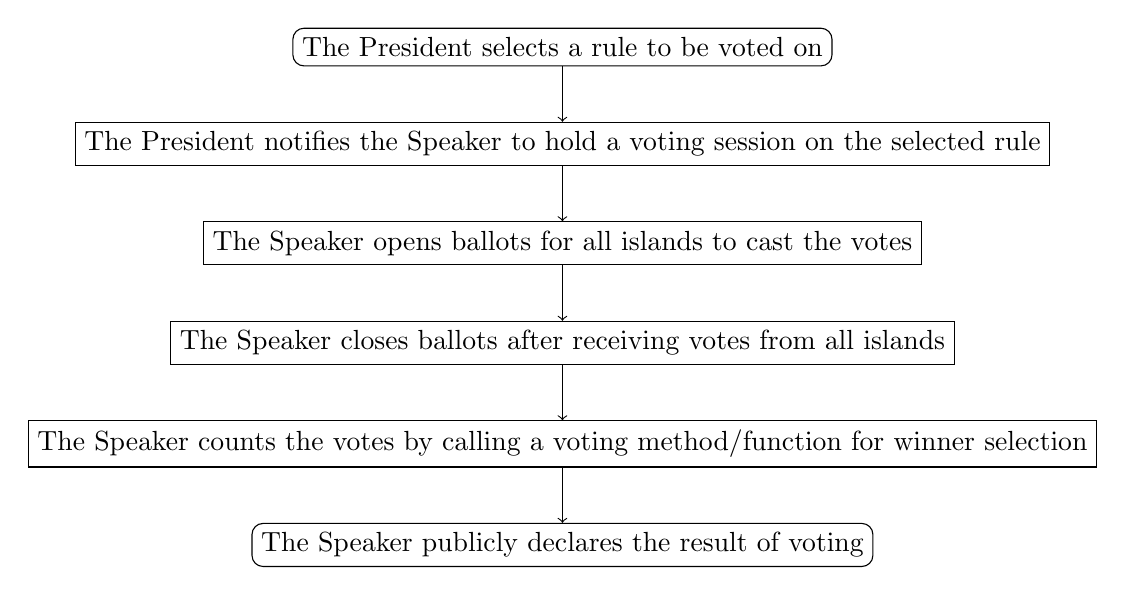
\begin{tikzpicture}[node distance=20pt]
\centering
\node[draw, rounded corners] (start)  {The President selects a rule to be voted on};
\node[draw, below=of start] (step 1)  {The President notifies the Speaker to hold a voting session on the selected rule};
\node[draw, below=of step 1] (step 2)  {The Speaker opens ballots for all islands to cast the votes};
\node[draw, below=of step 2] (step 3)  {The Speaker closes ballots after receiving votes from all islands};
\node[draw, below=of step 3] (step 4)  {The Speaker counts the votes by calling a voting method/function for winner selection};
\node[draw, below=of step 4, rounded corners] (end)   {The Speaker publicly declares the result of voting};
 \draw[->] (start)  -- (step 1);
 \draw[->] (step 1) -- (step 2);
 \draw[->] (step 2) -- (step 3);
 \draw[->] (step 3) -- (step 4);
 \draw[->] (step 4) -- (end);
\end{tikzpicture}
\caption{Voting Protocol for Rules}
\label{fig:RONRVotingProtocol}
\end{center}
\end{figure}

For elections of roles, the sequence of actions of the voting protocol is mostly similar to the above explanation in principle, except for some parameters, such as the motion of the vote which is the role itself (President, or Speaker, or Judge), the facilitator of the election/vote event which depends on what role is being held for election (refer to Chapter 5 IIGO for more details on change of roles and power transfer), and the applicable voting method function to call for election that will produce the result, which is different from the voting method used for rules. Refer to Section~\ref{sec:VotingMethods} for more details on voting methods to be used for elections of roles.

In the initial implementation, it is assumed that all 6 islands have the power to vote at any necessary voting scenario and no sanction or power restriction applied to any island when it comes to the right to vote. However, in the final implementation, some complications or dilemma are applied to, i.e. an/some island(s) could lose their right to vote or not permitted to participate in a voting event due to diplomatic sanction. Refer to Chapter 5 IIGO for details on diplomatic sanction. In this case, the Speaker will check and open the ballots to only eligible islands that have the right to vote at that certain stage, rather than to all islands as mentioned in the first scenario above.

\section{Implementation}
\label{sec:Implementation}

\subsection{Voting for Rules}
\label{sec:VotingForRules}
The implementation of voting for rules from infrastructure point of view (file:\texttt{rulevote.go}) basically follows the sequence of voting protocol as described in Section~\ref{sec:VotingProtocol}. At initialisation, there are two defined structs (collection of data fields) that are used as parameters for functions inside the voting algorithm, such as \texttt{RuleVote} and \texttt{BallotBox}. The \texttt{RuleVote} struct consists of 3 variables, i.e. \texttt{ruleToVote} (string) that contains the rule that has been selected by the President to be voted on, \texttt{islandsToVote} (list of integers) that contains a list of \texttt{ClientID} which indicates all eligible islands that participate in the voting session, and \texttt{ballots} (list of boolean) that contains the vote of each respective eligible islands where it can indicate the vote for in-favour or against the proposed rule. The \texttt{BallotBox} struct consists of 2 integer variables that act as accumulators for the count of each possible vote: \texttt{VotesInFavour} and \texttt{VotesAgainst}.

According to Section~\ref{sec:VotingProtocol}, The Speaker firstly starts a voting session by calling \texttt{SetRule(rule)} function that contains the rule selected by The President to be voted on. Next, the Speaker sets all eligible islands that can participate/have the right to vote in the voting session at that state of the game by using \texttt{SetVotingIslands(clientIDs[])} function. After that, the Speaker opens the ballots to get the votes from all eligible islands by calling \texttt{GatherBallots(clientMap[ClientID])} function. Subsequently, the \texttt{GetBallotBox()} function is called by the Speaker to gather the ballots that already contain the votes counting of those who are in-favour or against the proposed rule. Finally, the votes counting is concluded by comparing the votes of those in-favour vs those against, and the in-favour votes win when the counting is greater than or equal to the against votes counting, as reflected in \texttt{CountVotesMajority()} function. The Speaker then uses this result to declare the result of this voting session in IIGO.

\subsection{Elections}
\label{subsec:Elections}
The elections for roles implementation can be seen in the file:\texttt{election.go}. At initialisation, there is a defined struct \texttt{Election} that contains 4 parameters, i.e. \texttt{roleToElect} that indicates which role is being voted on (President, or Speaker, or Judge), \texttt{votingMethod} that indicates the voting method being used for the election to determine the winner selection, \texttt{islandsToVote} that contains a list of \texttt{ClientID} which indicates all eligible islands that participate in the voting session, and \texttt{votes} that is a list that contains the order rank of preference of the candidates for the role from each eligible island who casts the vote.

The election session begins by calling the \texttt{ProposeElection(role,method)} function that depends on which role being voted on and which role has obligation to facilitate the election (refer to Chapter 5 IIGO on Change of Roles and Power Transfer sections), and the selected voting method to be used for this election (refer to Section~\ref{sec:VotingMethods} for details on voting methods and Subsection~\ref{subsec:VotingPseudo} for pseudo-code implementation). The election facilitator then opens ballots to all eligible islands to cast their votes by calling \texttt{OpenBallot(clientIDs[])} function. The \texttt{Vote(clientMap[ClientID])} function gathers all the ballots containing the votes from all eligible islands that are obtained from \texttt{GetVoteForElection(roleToElect)} function returned from each client/island code execution. After that, the election facilitator closes the ballots by using \texttt{CloseBallot()} function and it returns the result of the votes counting using the selected voting method by calling each respective voting method function. This result is used by the election facilitator to declare the winner for the elected role. By default, the voting method for election is Borda Count and the function is called \texttt{bordaCountResult()} where the algorithm follows through what are explained in Section~\ref{sec:VotingMethods} and Subsection~\ref{subsec:VotingPseudo} where the Borda scores will be calculated based on the order rank of preference of the candidates from each ballot. The other voting methods can be used for election and it is selected by the election facilitator.

\subsection{Voting Methods Implementation Pseudo-code}
\label{subsec:VotingPseudo}

\textbf{Plurality}
\newline
Call for Voting inputs (int:IslandID, str:"Aye", "Nay" or "Abstain")\\
\begin{algorithm}[H]
\ForEach{$ballot \in ballots $}{
    \If{$Aye$} {Count for $Aye ++ $}
    \If{$Nay$} {Count for $Nay ++ $}
}
\If{$Aye > Nay$}{\Return the Winner: $Aye$}
\Else{\Return the Winner: $Nay$}
\end{algorithm}

\ \newline \ \newline \ \newline
\textbf{Borda Count}
\newline
\begin{algorithm}[H]
\For{all ballot}{
    $numNotIn\gets N-ballot.length$\\
    $shareScore\gets 1+...+numNotIn$\\
    \For{i from 0 to N-1}{
    \If{i is in ballots} {$scores[i]\gets scores[i]+N-K+1$ }
    \Else {$scores[i]\gets scores[i]+shareScore/numsNotIn$ }
    }
}
Sort candidates by Borda scores\\
\Return the candidate with the highest score
\end{algorithm}

\ \newline \ \newline \ \newline
\textbf{Runoff}
\newline
\begin{algorithm}[H]
\For{All $ballot \in ballots $}{
    Select two candidates with most first-placed votes
}
\If{either already has a majority}{
\Return the majority one}
\Else{Each voter selects one candidate of the top 2\\
}
\Return the candidate with the most votes
\end{algorithm}

\ \newline \ \newline \ \newline
\textbf{Instant Runoff}
\newline
\begin{algorithm}[H]
\ForEach{$ballot \in ballots $}{
\For{i from 0 to N-1}{
\If{i is first choice}{$scores[i]\gets scores[i]+N-K+1$}
}
}
\If{candidate in ballots $>1$}{
Remove the candidate with the fewest first
choice votes from the ballots.\\
GOTO the top for next round of counting
}
\Else{\Return the candidate}
\end{algorithm} 

\ \newline \ \newline \ \newline
\textbf{Approval}\\
\begin{algorithm}[H]
\ForEach{$ballot \in ballots $}{
    \For{i from 0 to N-1}{
    \If{i is in ballot} {$scores[i]\gets scores[i]+1$ }
    }

}
Sort candidates by scores\\
\Return the candidate with highest score
\end{algorithm}

    \chapter{Team 1 Agent Design}

\section{Core Idea}
Team 1 Agent was designed around the idea that the agent wants the whole archipelago to survive. However, the agent does have different configurations that allows it to be more malicious than intended such that interesting simulations may occur.

\section{Opinions on Islands}
For an agent to become self-organising, the agent must determine certain actions given a condition without external input. For this to be possible, the agent must have defined conditions which team 1 calls 'emotional state', and hold an opinion about other islands. This will form a basis for the agent to decide on an action.

Initially, the opinion on all existing islands are neutral. Overtime through IITO and IIGO, the opinions on islands will change. This will affect the outcome of IITO and IIGO results. As a note, positive values correspond to positive opinions while negative values correspond to negative opinions.

An agent's emotional state can change depending on the current resources. Below is an example of how an agent's emotional state can be formed:
\begin{itemize}
    \item If current resources > 10 * living cost, the agent is happy.
    \item If 3 * living cost < current resources < 10 * living cost, the agent is anxious.
    \item If the current resources < 3 * living cost, the agent is desperate.
\end{itemize}
The upper and lower bounds can be changed before a game starts. 

\section{IITO Gifts}
During IITO, the agent's opinion of other island is affected. For every gift received, the agent's opinion of the gifter increases. However, the agent's opinion of an island can decrease if that island promised a gift and was not able to fulfil it. 

When team 1 agent receives a request for gifts, the agent will decide how much to offer depending on the agent's current emotional state and the opinion of that island. 

\begin{table} [htb]
    \centering
    \begin{tabular}{|c|p{0.5\textwidth}|}
        \hline
        Emotional State & How is IITO handled? \\
        \hline
        Happy & Agent will give away its resources that satisfies the requested amount. \\
        \hline
        Anxious & Agent will give away a ratio of the requested amount and its current resources. \\
        \hline
        Desperate & Agent will refuse any gift requests that it receives. \\ 
        \hline
    \end{tabular}
\end{table}

Moreover, if the agent's opinion of an island is very high, the agent can decide to give gifts disregarding the agent's own anxiety. On the other hand, if an opinion of an island is very low, the agent can decide to refuse to send a gift even though the agent is happy. 

For increase survivability, team 1 agent will accept any gift offers that it receives. 

\subsection{Future Works}
Team 1 agent currently has a very straight-forward IITO strategy. Some interesting alteration to this strategy could include:
\begin{itemize}
    \item Being less suspectible to bribery. The agent should stop increasing the opinion of an island after receiving $X$ amount of continuous gifts.
    \item Stop handing out gifts to islands that are not in critical state.
    \item Being proactive in bribery. The agent will give unrequested gifts to the current president in hopes that this will reduce tax and increase resource allocation from the common pool. 
\end{itemize}

\section{IIFO Disaster Prediction}
Disasters can happen deterministically or stochastically (mentioned in detail in Chapter~\ref{sec: Disaster} for more information). For an agent, it is important to determine when a disaster occurs so that as much disaster damage is mitigated using the common pool. 

When the game starts, the disaster prediction made by the agent is random. This prediction always has a confidence value of 0. As more disasters occur, a history of disasters is built up. Using this history, the mean disaster position x, position y, magnitude and occurrence is calculated. A confidence value is calculated along with the mean disaster metrics. 

% Add a footnote on website?  https://www.mathsisfun.com/data/confidence-interval.html
The confidence value is calculated by finding the ratio between margin of error and the mean value. The smaller the margin of error, the more confident the agent is. Therefore, a difference between the mean value and the margin of error must also be calculated. To begin with, the agent uses the confidence interval equation (where $s =$ standard deviation, $n = $ size of array, $Z = $ confidence interval) to calculate the margin of error:
\begin{equation}
    \label{eq: Team1MarginOfError}
    \text{Error} = Z \dfrac{s}{\sqrt{n}} 
\end{equation}
Using the difference between the mean value ($\bar{x}$) and the margin of error along with finding out the ratio of this result will provide the agent with the confidence value.
\begin{equation}
    \text{Confidence Value} = (\bar{x} - \text{Error}) \times \dfrac{1}{\bar{x}}
\end{equation}

Sharing and obtaining other disaster information to and from other islands respectively can increase the survivability of the archipelago. As more disaster prediction is shared, a network of trust between team 1 agent and other island is built. This trust value is primarily based upon the absolute value of the islands prediction on the day the disaster happened. However, if an island shares a disaster prediction with the estimated disaster day to be random or changing erratically each turn, then team 1 agent will begin to distrust that island. 

\section{IIGO: President}

\section{Foraging}
Multiple foraging strategies were developed: 
\begin{itemize}
    \item Return on Investment (ROI)
    \item Regression
    \item Flip Forage
\end{itemize}

\subsection{Simulations against ourselves}

Multiple foraging strategies were developed, initially by intuition and later by attempting to address the shortcomings of previous attempts:

\subsection{Return on Investment (ROI) Foraging}%
\label{sec:forage-roi}

This first algorithm is based on repeating successful foraging behaviours in the past, whether those be by the agent herself or another agent.

For the first few turns (the exact amount is configurable) the agent will forage randomly.

The agent maintains a history of foraging decisions and outcomes, including those received from IIFO.\@ When it comes time to forage this history is sorted by ROI, i.e.\ the ratio of profit to contribution. Decisions that resulted in a loss, had profit smaller that the living cost, or had a larger contribution that a (configurable) percentage of available resources are filtered out.

\subsection{Regression Foraging}%
\label{sec:forage-regression}

This strategy tries to predict the ideal foraging decision, even if that exact decision was not made in the past. This is done using regression, which is used to find the decision with the highest expected reward.

% In detail, history is kept as in \nameref{sec:forage-roi}. To make a foraging decision, the history is split by foraged resource (fish or deer), and quadratic regression is performed on contribution versus reward. The maximum of the regression curve is found for each group and the contribution with the highest

\subsection{Flip Foraging}

This strategy chooses the least foraged resource from the last turn, according to IIFO-reported data. Contributed amount is proportional to the chosen resource's total ROI from last turn. This choice was made under the assumption that ROI is an indicator of the resource's ``condition''. If a resource only gives moderate rewards (proportionally to input) it means that it is probably over-used currently and as such agents should allow it to recover, by scaling down their foraging attempts.

\subsection{Comparison}

To compare the three strategies, simulations were run with six agents, two using \emph{ROI foraging}, two using \emph{regression foraging}, and two using \emph{flip foraging}. IIGO and IITO were also disabled in order to isolate the efficacy of foraging methods from other parts of the game. The simulation was run five times and the results averaged over the 5 games as well as the two agents following the same strategy.

\begin{figure}[H] 
\centering
\includegraphics[width=0.6\textwidth]{09_team1_agentdesign/images/mean_survival_turns}
\caption{Mean survival turns for different strategies.}
\label{fig:team1:mean_survival}
\end{figure} 

\begin{figure}[H] 
\centering
\includegraphics[width=0.6\textwidth]{09_team1_agentdesign/images/total_efficiency}
\caption{Average foraging efficiency}
\label{fig:team1:average_efficiency}
\end{figure} 

It is clear from \autoref{fig:team1:mean_survival} that the \emph{flip} foraging strategy dominates the other two in terms of overall effectiveness. However, it is interesting to note that, according to \autoref{fig:team1:average_efficiency}, the \emph{ROI} foraging method is almost as efficient as \emph{flip}, which raises the question of what causes the difference in their success. This difference could be attributed to one core issue with the \emph{ROI strategy}: ignoring the absolute value of rewards. The agent will happily settle for a profit of $11$ resources, if that was obtained with a contribution of $0.1$ resources (a profit of $110000\%$) over a profit $50$ resources for a contribution of $25$ (a measly $100\%$). This means that in the long run living costs overwhelm the \emph{ROI} agent. The \emph{flip} agent does not take expected profit into account and as such is unaffected by this.

\emph{Regression} appears to occupy a medium between \emph{flip} and \emph{ROI}, however it is much less consistent, as evidenced by the error bars in \autoref{fig:team1:mean_survival}, with \emph{regression} surviving for under 10 turns in some runs.

%%% Local Variables:
%%% mode: latex
%%% TeX-master: "../main"
%%% End:

    \chapter{Team 2 Agent Design}
\section{Overall Agent Strategy}

The overall strategy of our agent is based on a series of distinct, overlapping dilemmas. The agent operates on principles based on Evolutionary Economic Theory \footnote{https://www.cambridge.org/core/what-we-publish/elements/evolutionary-economics}. Game theory and the use of the Nash equilibrium also guided the development of the strategies implemented. The other top-level strategy which overlaps with several dilemmas is the social dilemma; this is when we quantify the relationship we have with other agents to produce trust and confidence levels. The interaction between the top-level strategies with all of the dilemmas is shown in Figure~\ref{fig: top level strategy}. The top-level strategy's implementation into each agent function and role is discussed in the following sections. 

\begin{figure}[!htb]
    \centering
    \begin{subfigure}{.49\textwidth}
        \centering
        \includegraphics[width=0.99\textwidth]{images/strategies.png}
        \caption{Top level strategy}
        \label{fig: top level strategy}    
    \end{subfigure}
    \begin{subfigure}{.49\textwidth}
        \centering
        \includegraphics[width=0.9\textwidth]{images/dichotomy.png}
        \caption{Ceremonial-Instrumental dichotomy}
        \label{fig: dichotomy}
    \end{subfigure}
\end{figure}

\subsection{Evolutionary Economic Theory}
The term Evolutionary Economic Theory was first coined by economist Thorstein Veblen \footnote{https://www.cambridge.org/core/what-we-publish/elements/evolutionary-economics}. Evolutionary Economic Theory proposes that economic processes evolve, and it rejects the assumptions of classical rational choice theory. From Evolutionary Economic Theory, we categorised agent behaviour into distinct groups \footnote{https://www.cambridge.org/core/what-we-publish/elements/evolutionary-economics}. These groups are an altruist, fair sharer, and free rider. These are explained in Table~\ref{tab:Evolutionary Economic Theory Agent classifications}.

\begin{table}[!htb]
\caption{Evolutionary Economic Theory Agent classifications}
\label{tab:Evolutionary Economic Theory Agent classifications}
\begin{tabular}{|c|c|l|}
\hline
\textbf{Agent classification} & \textbf{Definition}                                                                                                                        & \multicolumn{1}{c|}{\textbf{Examples within the game}}                                                                                                        \\ \hline
Altruist                      & \begin{tabular}[c]{@{}c@{}}More concerned about the welfare \\ of the group than themselves\end{tabular}                                   & \begin{tabular}[c]{@{}l@{}}-Contributes a surplus to the common pool\\ -Generous with gifts\end{tabular}                                                     \\ \hline
Fair Sharer                   & \begin{tabular}[c]{@{}c@{}}Contributes enough to the group \\ to negate their negative impact on it\end{tabular}                           & \begin{tabular}[c]{@{}l@{}}-Contributes the minimum necessary amount of resources \\ -Gift allocation is measured and reasonable\end{tabular}                          \\ \hline
Free rider                    & \multicolumn{1}{l|}{\begin{tabular}[c]{@{}l@{}}More concerned with their individual \\ welfare than the welfare of the group\end{tabular}} & \begin{tabular}[c]{@{}l@{}}-Will not contribute enough to the common pool \\ -Gift requests above their requirement \\ -Will not give out gifts\end{tabular} \\ \hline
\end{tabular}
\end{table}

The advantage of using this theory over rational choice theory from classical economics is that it accounts for the irrational decisions agents or humans make when dealing with economic decisions, such as deciding how much to contribute to a common pool. Humans have evolved to develop heuristics \footnote{https://www.sciencedirect.com/topics/social-sciences/heuristics} which are "rules of thumb" in order to make economic decisions quickly and when all information is not present. These heuristics are typically based on emotion and will often result in irrational decisions; an example of this would be brand loyalty. This is very relevant within the context of the game because there is a cost to large computations (decision making). Also, there is an information failure \footnote{https://www.economicsonline.co.uk/Market_failures/Information_failure.html} as the agents often do not know the threshold of the common pool and other vital game metrics. This information failure forces agents to use heuristics similar to those used by real people. An excellent example of a heuristic within this agent strategy is the level of trustworthiness decided within the social dilemma. If every agent was rational and all information was present in the game, there is no need to trust or distrust agents as they would maximize both their welfare and that of others.

Another primary reason for selecting this theory as the basis of our design is to explore the ceremonial-instrumental dichotomy\footnote{https://www.jstor.org/stable/3486187?seq=3#metadata_info_tab_contents}. This dichotomy is best represented by the graph in figure \ref{fig: dichotomy} and shows the importance of the game's setup. Our agent is attempting to oppose this traditional response to instrumental and ceremonial societies. It would be interesting to change the game's ceremonial and instrumental values by changing the setup. While the current game infrastructure does not support this, it would be interesting to investigate the ceremonial-instrumental dichotomy by allowing islands to invest resources into developing their foraging technology to obtain higher returns. It would be interesting to investigate how this instrumental shift would change our agent's strategy and others' actions. This update in technology would replace the ceremonial institutional set up of the IIGO as it becomes redundant. Allowing islands to invest in technological advancement would add an extra dimension to the game as it evolves, and the importance of the IIGO and other instrumental components would shift.

\subsection{Evolutionary Economic Theory Implementation}
%explain how we use the information from the theory

Figure~\ref{fig:methods-of-play} shows the different states of our agent's different methods of play. At any point during the game, the state of our agent is determined only by the level of the Common Pool. Our agent's objective is to oppose the strategies employed by other agents to attain stability in the game. To determine the method of play of the other agents, we look at whether the Common Pool is, on average, increasing or decreasing. If the pool is being depleted, it can be assumed that the other agents act as free-riders on average. To counteract this, we act as an altruist (see section \ref{sec:Common Pool Dilemma Strategy} for more detail). The average pool level is used because individual agent strategies are irrelevant for the game's overall course. Within the game, we also do not always have access to individual agents' contributions, which would be needed to classify them individually. This makes the average level of the Common Pool the only viable parameter. 

Our simulations demonstrated that starting the game in a "free-rider" state resulted in optimal agent performance and did not negatively impact the course of the game overall.

The default state for the agent is to be a "fair sharer." The agent will move into altruist mode when the weighted average of the Common Pool has dropped drastically. The agent considers a weighted average to ensure that the agent does not panic after every disaster and over contribute. The most recent turns will also be weighed higher to determine the course of the game. When the Common Pool stops decreasing, the agent will move back to fair sharer mode. Similarly, if the pool's weighted average increases by a large factor, then our agent moves into a free-rider state.

\begin{figure}
\centering
\begin{subfigure}{.49\textwidth}
    \centering
    \includegraphics[width=0.9\textwidth]{images/MethodofPlay.png}
    \caption{Method of Play diagram}
    \label{fig:methods-of-play}
\end{subfigure}
\begin{subfigure}{.49\textwidth}
    \centering
    \includegraphics[width=0.9\textwidth]{images/Social.png}
    \caption{Social Classification Order}
    \label{fig:social-order}
\end{subfigure}
\end{figure}

\subsection{Social Classification}
The agent forms an opinion on others depending on different situations. Initial testing suggested that another island's gift-giving behaviour does not necessarily correlate with their quality of predictions. Consequently, the trust of other agents is computed and stored separately for each situation. The agent uses the weighted average of past interactions with other agents to determine whether or not to trust them in each situation for future interactions. Using a weighted average to compute trust resulted in notably better agent performance. This is because the agent's trust in other agents considers all interactions with other agents while weighting recent interactions more heavily.

An integer value represents the agent's trust metric for each agent in each situation between 0 and 100, where 100 denotes full confidence and 0 a complete lack thereof. This value is used to compute the expected outcomes of situations. These are then compared with real events to update the agent's confidence in the other agents regarding this situation. For example, when the agent receives predictions from other islands, it computes the weighted average to check whether it trusts the island. Once a disaster occurs, the magnitude or timing of the disaster is compared with the other island's prediction. This reality is used to assess their behaviour and update the trust metric for that island relating to that situation. The list of different "situations" includes how an agent behaves in a role such as the President, Judge, Speaker, gift-giving, and disaster prediction. The overall structure of how the agent forms opinions on other islands is shown in Figure~\ref{fig:social-order}.

\section{Gift Giving and Receiving}
The agent must decide whether or not to respond to other agents' gift requests and how much to request from others through gifting. The implementation does not consider whether or not an agent is critical when requesting gifts and instead considers its current method of play and the trustworthiness of the requesting agent. Figure~\ref{fig: gifts} shows a decision tree for how the agent will allocate or request gifts, in which the agent splits up the gift request among the other agents to increase the likelihood of an agent allocating the gift.


\begin{figure}[!htb]
    \begin{subfigure}{.49\textwidth}
        \centering
        \includegraphics[width=0.99\textwidth]{images/gifts.png}
        \caption{Gift Giving and Receiving decision tree}
        \label{fig: gifts}
    \end{subfigure}
    \begin{subfigure}{.49\textwidth}
        \centering
        \includegraphics[width=0.99\textwidth]{images/common_pool_strategy.png}
        \caption{Common Pool Strategy}
        \label{fig: common_pool_strategy}        
    \end{subfigure}
\end{figure}

Depending on the method of play, the agent will request more or fewer gifts. This is inversely proportional to the number of resources taken from the Common Pool. The agent obtains a larger proportion of its needed resources from gifting than the Common Pool in the altruist state. This is done to mitigate common pool depletion in the interest of the common good. In a Fair-Sharer state, the agent aims to obtain its resource target equally from gifts and the Common Pool. A minor surplus is also included in the resource target to ensure that the goal is met, given that gifts from other agents cannot be guaranteed. In a Free-Rider state, the agent takes the majority of its resources directly from the Common Pool but still requests gifts to build up its resources by taking advantage of relationships with other agents as well as a Common Pool surplus.

The \textbf{Gifts} social classification situation refers to both when an island requests a gift from our agent and when our agent requests a gift from that island. The balance between agent gift requests and responses is used as a basis for opinion formation on another agent. Other agents that fulfill the agent's requests are rewarded with higher trust. The agent's own gift requests tend to be small but are also proportional to its trust in each other agent. Every gift interaction is used to update the agent's trust in another island's gifting behaviour.

\section{Common Pool Dilemma Strategy} \label{sec:Common Pool Dilemma Strategy}
The Common Pool dilemma strategy can be split into two considerations. One consideration is the current method of play (altruist, fair sharer, and free-rider), and the other is the current game state. A decision tree showing the common pool strategy is shown in Figure~\ref{fig: common_pool_strategy}. These considerations decide whether and how much we contribute or take from the Common Pool.

\subsection{Method of play consideration} \label{ssec:Method of play consideration}
The primary consideration for giving to the Common Pool dilemma is the agent's current method of play. The agent's state is determined by the Common Pool level, as seen in Figure~\ref{fig:methods-of-play}. The agent's default state as a "fair sharer" contributes the average amount of other agents to the Common Pool. This is calculated by evaluating changes in the Common Pool level from the previous turn and averaging this quantity by dividing by the number of alive agents. If the Common Pool level decreases, the most recent Common pool increase is used to determine the amount given.

By using the average Common Pool contribution, the agent benefits from the forecasting of other agents. This benefit would arise should another agent have an advanced forecasting prediction that determines the Common Pool threshold and what is required to mitigate the effects of a disaster. In this case, the agent would then contribute a similar quantity of resources. This "herd-mentality" approach relies on the assumption that other agents make rational decisions. So if it is evident that other agents are acting irrationally, the agent deviates from this approach to an alternative state (to become either a free-rider or an altruist).

The agent is in an altruist state when the Common Pool is struggling, which often means that other agents act as free-riders. This is where the meta-strategy of Evolutionary Economic Theory comes into play. It is in the agent's interest to contribute much more to the Common Pool to alter the game's course in a positive direction and prevent the pool from being below the threshold when a disaster occurs. Therefore, the agent contributes more resources to enact this balance on the system. 
The altruist resource contribution is a larger factor of the weighted average contribution and can be tuned using the \emph{altruist factor} variable in the agent's configuration.

In a free-rider state, the Common Pool has a surplus, and the agent assumes other agents are on average operating as altruists. In this situation, the agent contributes less to the Common Pool and preserves resources to mitigate short and long-term risk. Contributing too much to the Common Pool no longer benefits the greater good, as these resources can still be used to forage and generate more resources. Therefore, the agent accumulates resources when others are too generous, allowing greater foraging investments and making it easier to help other agents if they struggle in the future.

The method of play also impacts how the agent decides to take from the Common Pool. After game state considerations are made, the agent adjusts how much it takes from the Common Pool according to its Agent State. Table~\ref{tab:Method of play common pool taking} outlines a summary of how the agent adjusts how much it takes and gives a justification for each action. The amount to take from the pool depends on how willing other agents are to contribute to the agent within the game's gift-giving section.  This means the agent must decide what proportion of the resource request must be taken from the Common Pool and from gifting, and this decision also factors in both common pool allocation as well as gift response predictions. When the agent is in a free-rider state, the common pool has a surplus, and so it makes more sense to take directly from the pool rather than requesting gifts. 

\begin{table}[!htb]
\centering
\caption{Method of play common pool taking}
\label{tab:Method of play common pool taking}
\begin{tabular}{|c|c|}
\hline
\textbf{Agent classification} & \textbf{How this impacts taking from the common pool}                              \\ \hline
Altruist                      & Pool is being depleted, best to not take from the pool                             \\ \hline
Fair Sharer                   & Gift requests and taking from the pool are equal                                   \\ \hline
Free rider                    & \multicolumn{1}{l|}{Pool has surplus, take from the pool rather than gift request} \\ \hline
\end{tabular}
\end{table}

\subsection{Game state consideration} \label{ssec:Game state consideration}
The primary consideration in taking from the Common Pool is the current game state. The key parameters (shown in Figure~\ref{fig: common_pool_strategy}) considered are whether the agent is critical and whether the agent has excess resources. This excess is calculated as the difference between the agent's current resources and the minimum resource threshold and the cost of living. Beyond this minimum resource level, the agent can survive one another turn. If the agent has fewer resources than these aggregated costs, the excess is zero. If there are excess resources, the agent will give some resources to the Common Pool. In this case, a strategic contribution is calculated. If the Common Pool threshold is known, the agent considers how many resources are required to attain this threshold. This is then spread over the expected number of turns until the next disaster is predicted to occur and the number of alive clients. If this is unknown, a default value is used to form an initial guess in the agent configuration. On top of this quantity, a strategic contribution is also calculated (see \ref{ssec:Method of play consideration}). The current method of play determines whether the disaster-determined contribution or the strategy-determined contribution is contributed to the pool. This amount is then contributed together with the current tax, unless there are no excess resources as this implies the agent is in a critical state and so all resources are preserved.

\section{Foraging Dilemma}
The foraging dilemma is split into two parts. One determines whether the agent should hunt or fish, and the other determines how many resources to spend on foraging. The foraging dilemma only depends on the current method of play. The method of play will impact the amount the agent uses to forages. If the Common Pool is doing well and the agent acts as a free rider, it will be more prone to take risk and contribute more to the foraging and vice versa. The decision to hunt or fish depends on the likely number of hunters in the next foraging event. The decision tree, Figure~\ref{fig: Hunt or fish decision tree }, shows how the agent decides whether to hunt or fish in a given turn. To determine the number of hunters in the next forage turn, the agent tracks how often each agent is a hunter and then sums up the probability of each agent hunting to find an overall number of likely hunters. The agent outputs a random number from 0 to 1, and if the number lies above the threshold, the agent will hunt. This threshold is determined by the number of likely hunters in the foraging. It implies there is an element of randomness to the agent's decision making, which will account for the unpredictability of dealing with other agents with their strategies.

\begin{figure}[!htb]
    \centering
    \begin{subfigure}{.49\textwidth}
        \centering
        \includegraphics[width=0.9\textwidth]{images/forage_decision.png}
        \caption{Hunt or fish decision tree }
        \label{fig: Hunt or fish decision tree }
    \end{subfigure}
    \begin{subfigure}{.49\textwidth}
        \centering
        \includegraphics[width=1.0\textwidth]{images/Roles Decision Tree.png}
        \caption{Roles Decision Tree}
        \label{fig: Roles Decision Tree}        
    \end{subfigure}
    \caption{Hunting or Fishing and Roles Decision Tree}
\end{figure}

The ideal distribution for foraging is to have two agents hunting and the remainder fishing. Hence, when the agent predicts one other agent will hunt, the agent is highly likely to choose to hunt too. The default threshold for hunting is 0.1, so the agent will hunt 10\% of the time when not considering the likely number of hunters. By assuming that any agent will hunt or fish with equal probability, the likelihood that there is one hunter is approximately 0.16. This implies hunting is an optimal strategy approximately 16\% of the time, so a threshold similar to this value is chosen. If the predicted number of hunters is above one, the following equation is used to determine threshold placement: $\text{Probability of agent hunting} = 0.95 - \text{Predicted number of hunters} \times 0.15$

The probability of choosing to hunt when the agent is confident only one other agent will also select hunt is 0.95. For each additionally predicted hunter, the probability will fall by 0.15. This 0.95 threshold is included in the agent configuration so it can be edited without changing the code. Hence, the foraging decision can be tuned. The agent checks if there are any excess resources after considering the minimum resource threshold not to be critical and the cost of living. If there are no excess resources, no resources are spent on foraging. If there is an excess of resources, a percentage of this excess is used on foraging. This percentage is controlled in the agent configuration. This approach ensures the agent has enough resources to survive another round, even in the worst case scenario when foraging returns are minimal.

\section{Role Strategies}

Figure~\ref{fig: Roles Decision Tree} shows a decision tree of how the agent acts under the two roles implemented. Due to time constraints, the base client implementation was used for the Speaker. The President is responsible for allocating resources from the Common Pool based on agent requests. The agent uses game state variables such as their critical status to determine if another agent is worthy of their resource request and the agent's allocation method based on the method of play is outlined in Table~\ref{tab:President allocation method of play}. When the agent is in a free-rider state, it is more selfish, while when it is an altruist, more of the others agents requests are approved. If an agent is not critical, it is highly unlikely that the agent will allocate them their requested resources as the purpose of the Common Pool should be to primarily mitigate the effects of disasters. Resources are allocated on a need-first basis, taxed proportionally to an agents resource level, and the strategy to determine taxation includes an additional penalty tax for agents who do not declare their resource levels. When evaluating another President's performance, the agent considers the percentage change in tax, the percentage of how much the agent is allocated with respect to how much it requests, and how much the agent takes with respect to how much the President allocates it.

\begin{table}[!htb]
\centering
\caption{President allocation method of play}
\label{tab:President allocation method of play}
\begin{tabular}{|c|c|}
\hline
\textbf{Agent classification} & \textbf{\% of request given} \\ \hline
Altruist                      & 60                           \\ \hline
Fair Sharer                   & 50                           \\ \hline
Free rider                    & 40                           \\ \hline
\end{tabular}
\end{table}

The agent implementation of the Judge evaluates whether an agent has broken any rules, as it should. However, to model real world corruption, the agent does not sanction agents that break rules if it considers them to be highly trustworthy (i.e., with a trust score above 80\%). The agents behaviour as a Judge is also determined by its state; when the agent is a free-rider, it sanctions fewer islands. The \textbf{Judge}'s situation, similar to the President, is used by the agent to determine what island to vote for as Judge. This is done by checking the past sanctions the agent received and their duration, to maxmimise personal benefit. The \textbf{RoleOpinion} social classification situation is used when the agent is the Judge and must decide whether or not to pardon other islands' sanctions, whom to choose as the next President whether or not an island has adhered by the rules. The Judge receives information for each island, such as the difference between how much an island contributed to the common pool and how much said they would. The agent uses these differences as a Judge to determine whether or not an island is trustworthy. During a role election, the agent checks its trust in the candidates for the appropriate situation, i.e., the situation when an agent is "President" for a future Presidential election. The agent will return a list of candidates in decreasing order of preference determined by the social classification. To do this, the agent sorts the candidates in terms of how much it trusts them.

\section{Disaster Prediction}
It is important for the agent to be capable of predicting both the severity and timing of disasters, in order to effectively make decisions for contributing to both the common pool and gifting resources to other agents.

Since the simulation is constructed through a series of successive turns, the occurrence of disasters throughout the game can be seen as a Binomial distribution: $D \sim \text{Bin}(n,p)$. In this equation, $D$ describes the number of disasters that occur, $n$ is the number of turns played and $p$ is the probability of a disaster occurring on a given turn.

The aim of our agent is to estimate the number of turns between disasters. We will denote this random variable as $T_D$, with our agent's aim being to find $E[T_D]$. To do this, our agent must estimate $p$. Therefore we have programmed our agent to find the Maximum Likelihood Estimator of $p$ for a Binomial RV\footnote{https://stats.stackexchange.com/questions/191444/variance-in-estimating-p-for-a-binomial-distribution}: $\hat{p} = \frac{D}{n} = \bar{X}$, where $\bar{X}$ is the sample mean of the RV $X$. The expectation of $T_D$ can be estimated using\footnote{https://math.stackexchange.com/questions/1299465/proof-variance-of-geometric-distribution}: $\hat{\mu}_{T_D}= \frac{1}{\hat{p}} = \frac{1}{\bar{X}}$. Thus, this is the optimal estimator for our agent to predict the number of turns between disasters. Furthermore, the confidence that our agent has in this prediction should be inversely proportional to the variance of $T_D$, i.e. how much does $T_D$ vary from the expected value we have found above? The expression for this variance is given below$^2$: $Var(T_D)= \frac{1-p}{p^2}$. 

However, given that our agent does not know the actual value of $p$ used in the simulation, our agent instead estimates the variance using: $\hat{\sigma}_{T_D}^2= \frac{1-\hat{p}}{\hat{p}^2}$. Now that an expression for the estimate of this variance has been obtained, two questions remain: ``what about the variance in $\hat{p}$" and ``how is this variance translated into a confidence value?" The variance of $\hat{p}$ is given by the following expression: $Var(\hat{p})= Var(\bar{X}) = \frac{Var(X)}{n}$. As previously, we do not know the exact value of $p$, making a calculation of $Var(X)$ impossible. However, we can make use of the fact that $Var(\hat{p}) \propto \frac{1}{n}$, by making our agents confidence in the prediction proportional to $n$ also. Secondly, the fact that variance can take values $\in [0,\infty]$ but confidence must take a value $\in [0, 100]$ makes mapping the values of variance that our agent calculates, to a confidence level, challenging. The solution our team opted for was to cap the max value of variance to some value $v_{cap_{T_D}}$, before translating this variance into a corresponding confidence value. This process is given by the equation below: $\text{confidence}_{T_D} = 100 - \frac{100 \cdot \text{min}(\frac{\hat{\sigma}_{T_D}^2}{kn}, v_{cap_{T_D}})}{v_{cap_{T_D}}}$ 
where $k$ is the tuning parameter for altering the dependence of the confidence on $n$. 

\subsection{Magnitude Prediction}
Our agent's strategy for predicting the magnitude of the next disaster shares many similarities with the strategy discussed in the last section. However, the magnitude of the next disaster is now distributed with an Exponential distribution: $M \sim Exp(\lambda)$. Once again, start by finding the MLE for the parameter $\lambda$ \footnote{https://en.wikipedia.org/wiki/Exponential\_distribution}: $\hat{\lambda} = \frac{1}{\bar{M}}$. Now we seek to estimate the expectation of $M$: $\hat{\mu}_M = \frac{1}{\hat{\lambda}} = \bar{M}$. Similarly, the variance of this RV is also useful to estimate $\hat{\sigma}_{M}^2= \frac{1}{\hat{\lambda}^2}$. As previously, there is also a variance in our estimation of $\hat{\lambda}$ that must be taken into account by making our confidence in this prediction proportional to $n$. Thus, the following expression should be used for calculating the confidence in the magnitude prediction: $\text{confidence}_M = 100 - \frac{100 \cdot \text{min}(\frac{\hat{\sigma}_{M}^2}{gn}, v_{cap_M})}{v_{cap_M}}$, where $g$ is the tuning parameter for altering the dependence of the confidence on $n$. 

\subsection{Overall Prediction}
The overall prediction that must be shared with teams during the IIFO session requires the following information: location, time until next disaster, magnitude and confidence. For our prediction of location, the middle of the archipelago is always given since the probability of a disaster occurring at a given location is uniform across the archipelago, meaning that there is no optimal prediction formula. Using the findings presented in the above sections, the formulas our agent will use to form a prediction about the next disaster are as follows:

\begin{align*}
    &x_{coord} = x_{min} + \frac{(x_{max}-x_{min})}{2}, y_{coord} = y_{min} + \frac{(y_{max}-y_{min})}{2}, \text{conf} =\frac{\text{conf}_{T_D} + \text{conf}_M}{2} \\
    &\hat{\mu}_{T_D}=\frac{1}{\bar{X}}, \hat{\mu}_M = \bar{M} \\
\end{align*}

\subsection{Combined Prediction}
Generating our own prediction is only the first part of the prediction making process. The second stage is to make use of other island's predictions during the IIFO session and using the social classification to decide prediction accuracy. When considering how much emphasis to put on a given island's prediction, we make use of two factors: 1.) Our island's confidence in each other island's prediction making. 2.) Each island's confidence in their own prediction, $P_i \in [0,100]$. These two considerations are then combined to create an overall confidence factor.

\section{Simulations}
Every function and agent consideration has tuneable parameter which can be edited without changing the whole agent. Figure~\ref{fig: Forage Untuned} shows how our agent reacts when it plays against itself and the foraging parameters are untuned. As you can see the game is unstable and the agents have a low survival rate. This is caused by an over contribution to the foraging dilemma, there is a point of marginal return with the foraging dilemma and spending too many resources can be wasteful. 

\begin{figure}[!htb]
    \centering
    \includegraphics[width=0.6\textwidth]{images/Forage Untuned.png}
    \caption{Untuned Forage Simulation}
    \label{fig: Forage Untuned}
\end{figure}

Figure~\ref{fig: Forage tuned} shows how our agents plays against itself when the foraging parameters are optimised. The amount of excess resources spent on foraging is more reasonable in this simulation, this results in a much higher survival rate and a more stable common pool.

\begin{figure}[!htb]
    \centering
    \includegraphics[width=0.6\textwidth]{images/Forage tuned.png}
    \caption{Tuned Forage Simulation}
    \label{fig: Forage tuned}
\end{figure}

Figure~\ref{fig: altruist sim}  shows what happens when the agent plays itself and they are all altruists by default and do not move out of altruist. It can be seen that the agents over contribute to the Common Pool and are left with nothing to forage, this ends the game rather quickly. The simulation result was very similar for when all of the agents were free riders, the game would end in a couple of rounds after a lack of contribution to the common pool which caused impactful disasters.  This proves that being a free rider or altruist is not a rational decision and must be avoided. 
%the other graph is not really as expected so lets just keep it like this

\begin{figure}[!htb]
    \centering
    \includegraphics[width=0.7\textwidth]{images/altruist sim.png}
    \caption{Altruist simulation}
    \label{fig:  altruist sim}
\end{figure}
     \documentclass{article}

\usepackage[legalpaper, potrait, margin=1in]{geometry}
\usepackage[utf8]{inputenc}
\usepackage{gensymb}
\usepackage{graphicx}
\usepackage{float}
\usepackage{color,soul}
\usepackage[dvipsnames]{xcolor}
\usepackage{float}
\usepackage{array}
\usepackage{arydshln}
\usepackage{amsthm}
\usepackage{adjustbox}
\newtheorem{definition}{Definition}
\setlength\dashlinedash{0.2pt}
\setlength\dashlinegap{1.5pt}
\setlength\arrayrulewidth{0.3pt}
 
 \usepackage[linesnumbered,ruled,vlined]{algorithm2e}


 
 

\newenvironment{conditions}
  {\par\vspace{\abovedisplayskip}\noindent\begin{tabular}{>{$}l<{$} @{${}={}$} l}}
  {\end{tabular}\par\vspace{\belowdisplayskip}}


\title{Team 3: Pittstop Agent Strategy}

\begin{document}

\maketitle

\section{Introduction}

Team 3 was interested in the parallels between this project and human societies. We wanted to build an agent that was flexible enough to mimic the diverse personality traits of ordinary citizens, as well leaders in governments around the world.

Section~\ref{sec:overall_strat} discusses the foundation of parameters and methods the team wrote in its approach towards building the agent. Section~\ref{section_func_team3} details how the team used this foundation to implement the required functionality of the agent (i.e. roles, voting, prediction, gifting, foraging) in a way that is compatible with our goal of flexibility, without compromising efficiency or intelligence. Section~\ref{sec:team3_simulation} then elaborates on game simulations, in which the team decided to anthropomorphize the agent by modelling it after three famous historical and political personalities. Simulations consisting of different permutations of these personalities reveal interesting conclusions about the performance of the archipelago. Finally, Section~\ref{sec:management} concludes our report with information about project management.

\section{Overall Agent Strategy}
\label{sec:overall_strat}

\subsection{Overview}
\label{sec:overview}


The agent was created by first a set of high-level parameters, most of which were used as scaling factors throughout the code base of the agent, and some as Boolean values that turn on or off specific behaviours. These parameters hence govern the agents interactions with the rest of the game. The effect of each parameter on the behaviour of the agent is summarized in Table~\ref{tab:team3:parameter_effects}. \\


\begin{center}
    
\begin{table}[H]
\centering
\begin{tabular}{l|l}
\textbf{Parameters} & \textbf{Description}  \\ 
\hline
\texttt{equity}                       & controls the allocation distribution of resources amongst islands              \\ \hdashline
\texttt{resourceSkew}                 & factor to adjust resource allocation based on trust             \\ \hdashline
\texttt{complianceLevel}              & quantifies how often the agent cheata during the game             \\ \hdashline
\texttt{saveCriticalIsland}           & if True, our agent will try to save any critical island             \\ \hdashline
\texttt{selfishness}                  & quantifies how selfish our agent is (e.g. in the context of gifts)             \\ \hdashline
\texttt{riskFactor}                   & quantifies how much risk our agent is willing to take        \\ \hdashline
\texttt{friendliness}                 & quantifies how friendly we will be during agent interactions            \\ \hdashline
\texttt{sensitivity}                  & quantifies how sensitive the agent will be to external changes            \\ \hdashline
\texttt{giftInflationPercentage}      & factor to adjust when gift requests are made to other islands             \\ \hdashline
\texttt{advType}                      & enables the agent to exploit institutional powers when elected in a role    \\ \hdashline
\texttt{controlLoop}                  & boolean to enable the feedback loop for the agent       
\end{tabular}
\caption{List of global parameters that dictate our agent strategy.}
\label{tab:team3:parameter_effects}
\end{table}
\end{center}

\subsection{Core functions}

Based on these parameters, we also wrote a set of core functions which would be useful to all variations of the agent. These functions implement Opinion Formation and Compliance Calculation.


\subsubsection*{Opinion Formation} \label{section_opinion_formation}
In a game where there can be up to n-agents, \textit{opinion formation} allows our agent to quantitatively assess the behaviour of the others based on previous interactions. %The agent uses this information in the form of \textit{trust decision-making} to reduce uncertainties and ultimately maximise its returns during any activity. 
In our implementation, we use a \texttt{trustScore} map to keep track of the agent's trust in (n-1)-agents. This map is used in combination with other pre-configured parameters to make strategic decisions during a turn. 
Trust takes a score between 0 (lowest) and 100 (highest). At the beginning of the game, all trust scores are initialised at 50, representing a neutral opinion. In our implementation, the trust scores can change during the following game activities:

\begin{itemize}
    \item Gifting: When our agent receives gift offers (after requesting gifts) and actual gift amount(s) received.
    \item Role Evaluations: When our agent evaluates the performance of the President, the Speaker and the Judge based on their respective roles and responsibilities.
    \item Sanctions: When we receive the broadcast of sanction from the Judge outlining the sanctions placed for that turn.
\end{itemize}

%This mean that the more turns there are in a game, the more variation one will observe in the trust scores. They provide an effective source of perceived opinion for the agent to intelligently devise and choose a strategy in a given situation with limited external information. 

At every turn of the game, the agent will participate in multiple activities and hence, it would be counter-intuitive if the agent directly updated the \texttt{trustScore} map otherwise only the last score change would be retained. We thus implemented a local cache, \texttt{trustMapAgg}, to keep track of all trust score updates made during agent activities for that turn. 

In the following turn, the \texttt{trustScore} map is updated by averaging all cached trust score changes for each agent in play. This allows the agent to progressively accumulate knowledge while still forming independent opinions from the results of the activities in each turn. Trust scores are also bounded between 0 and 100 for consistency. The process (for a single turn) is summarized in Figure~\ref{fig:trust_scores}.\\

\begin{figure}[H] 
\centering
\includegraphics[width=0.75\textwidth]{figures/TrustScores.jpg}
\caption{Diagram showing the series of changes to trust scores during a single turn.}
\label{fig:trust_scores}
\end{figure}

%The \texttt{trustScore}  For example, when our island is elected as a Judge, the agent will rely upon these trust scores to determine which islands to pardon. This allows the agent to facilitate trust and forgiveness within the same framework.

\subsubsection*{Compliance Calculation}
Compliance Calculation determines at what point of the game it is most strategic to cheat. At every turn we calculate the \texttt{compliance} for the next turn\footnote{Note that \texttt{compliance} is how much our agent should comply at a given turn, while \texttt{complianceLevel} is how much our agent should comply during the entire game.}. The compliance calculation is based on the following principles:
\begin{enumerate}
    \item Every time we are caught, \texttt{compliance} is reset to 1.
    \item The more our agent is caught, the less it should cheat.
    \item If our agent has not been caught cheating for an infinite amount of turns, $\texttt{compliance}=\texttt{complianceLevel}$.
    \item The more our agent is caught, the longer it should take \texttt{compliance} to converge to \texttt{complianceLevel}.
\end{enumerate}

Those principles were converted into Equation~\ref{team3:eq:compliance}, shown here below:

\begin{equation}
    c(t,n)=\texttt{complianceLevel}+(1-\texttt{complianceLevel})\times e^{\frac{-t}{n+1}} \label{team3:eq:compliance}
\end{equation}

where:
\begin{conditions}
 c     &  \textttt{compliance} at a given turn \\
 t     &  time since the agent was last caught by a Judge (in number of turns) \\
 n    &  number of times the agent has been caught since the game started \\   
 \texttt{complianceLevel} &  target compliance - global parameters (see Table~\ref{tab:team3:parameter_effects})
\end{conditions}

Figure~\ref{fig:compliance_decay} illustrates how compliance decays based on the number of times caught. 

\begin{figure}[H] 
\centering
\includegraphics[width=0.4\textwidth]{figures/compliance_graph.pdf}
\caption{Compliance decay over several turns with $\texttt{complianceLevel}=0.3$.}
\label{fig:compliance_decay}
\end{figure} 

The agent, in various functions described in the following section, then decides whether or not to cheat by generating a random real number in $[0,1]$ and checking if it is lower than \texttt{compliance}.

% \begin{center}
%     \text{Let $X$ be a random number between 0 and 1,}
% \end{center}
% \begin{equation}
%   i.e.  X \sim U( [0,1]).
% \end{equation}

% \begin{equation}
%     if \; \texttt{compliance} < X \rightarrow \; cheat
%     \label{eq:should_I_cheat}
% \end{equation}

\subsubsection{Common State Variables}
In addition to the global parameters, a number of variables were also created to track the current state of the agent. These are accessed and updated by most functions throughout the agent's code base. 
\begin{itemize}
\item Gifting history
\item Trust scores for each island 
\item Performance score of each island for positions of power (i.e. the Speaker, Judge, President)
\item Number of times sanctioned
\item Cached information from IIGO (e.g. sanctions, monitoring outcomes and taxation/allocation)
\end{itemize}

\section{Implementation of agent-specific functions}
\label{section_func_team3}

This section covers how we implemented functions for each of the expected behaviours of the agent, as well as details of how they are affected by parameter changes.

\subsection{Voting}

\subsubsection{Voting for Rules}
Our rules are stored in the form of matrices, which opens up to our agent the geometric analysis of linear algebra. We observe that each rule matrix requires a number of inputs. These inputs may be considered to form $n-dimensional$ space. \\
As explained in Section~\ref{dynamics} below, our dynamics package is able to analyse these n-dimensional spaces and calculate whether a particular rule pushes us further from compliance or moves us towards a compliant position in this $n-dimensional$ space. Depending on whether the proposed rule brings us closer to compliance or not, we chose to vote for or against it.

\subsubsection{Voting for Elections}
At the end of each session of the IIGO, all islands need to submit votes for their preferences for the next Speaker, Judge and President. Since the vote is implemented using a Borda Count, teams are required to submit an ordered list of islands, ranked according to preference. 

We implemented voting by evaluating the performance of each island that held the positions of Speaker, Judge and President at the end of each IIGO session. Evaluations are performed using heuristics. Islands are ranked for each role based on the report from the accountability cycle and our interaction with the role during the turn. For example, if the Speaker chose the rule we suggested, they would have a better evaluation. However, if we get a smaller than requested allocation from the President, we would rank the island occupying the role lower.

\subsection{Environment}

\subsubsection{Foraging}
Foraging for our agent was implemented to maximise the return while maintaining a risk proportional to the \textttt{riskFactor} parameter. To achieve this, we use foraging results from previous turn from our island and the ones shared by other islands in  IIFO.
Our foraging strategy decision making ensures we are not in a critical state if foraging does not turn profitable.

At every turn, we follow the following strategy:

\begin{enumerate}
    \item Determine maximum foraging investment amount amount using the \textttt{riskFactor} parameter, our current resources and our estimation of the critical threshold.
    \item Set the maximum foraging investment amount based on our current resources and the minimum leftover resources amount.
    \item Compute the expected return of investment of both foraging techniques, hunting and fishing, using the stored history of past foraging returns. 
    \item If one foraging technique has a positive expected return, we compute a decay factor to adjust our investment based on what islands have chosen to forage in the last turn and how many dears/fishes were caught. This ensures that we do not hunt when the population is too low or that a lot of other islands are foraging with us.
    \item If no foraging technique is expected to be profitable, we only invest a small amount to get additional information in the next rounds and we don't take unnecessary risks.  
    \item The final amount we decide to forage is scaled by the risk factor parameter.
\end{enumerate}

This foraging decision making algorithm proved to be efficient and produces stable positive returns at different risk levels for our agent.

\subsubsection{Disaster Prediction}

Our agent predicts disaster using a combination of our own estimation of the disasters distribution and predictions from other teams.

Our estimation is obtained by computing the mean and variance of the coordinates, the magnitudes and the number of turns between past disasters. The variance is used to specify the confidence we have in our own prediction.

Other island's predictions are weighted based on their forecasting ability obtained by analysing their history of predictions of past disasters, the confidence they have in their own predictions as well as how much we trust them.

At each turn, we share our predictions with alive islands and store the ones from other teams. When a disaster occurs, we log this information to determine forecasting abilities of other islands.

\subsection{Trade}

The gifting session described provides four major phases for our agent to take part in. Trade is a two-way interaction and as per game sequence, it is the first opportunity (in every turn) to formulate an opinion.

\subsubsection{Gift Requests}
Our gift requests depend on 2 main parameters in our agent strategy, \texttt{giftInflationPercentage} and \texttt{riskFactor}, along with the \texttt{trustScore} map that we have built based on opinion formation of the other island. Essentially, we cover the risk that we do not get resources from the islands that we do not trust as much with what we get from islands that we do trust. Additionally, we do not request any gifts from critical islands in order to help them survive. \\

At every turn, we follow the following strategy:

\begin{enumerate}
    \item The resources our islands plans to ask for in gifts is calculated by finding the different between the \texttt{initialResourcesAtStartOfGame} and our \texttt{localPool}.
    \item If we actually need resources, we inflate the total requests that we make to account for differences in gifts we might actually receive. Otherwise, if do not actually need resources, we just request a percentage of \texttt{initialResourcesAtStartOfGame} for later opinion formation.
    \item We find the number of alive islands in the game and calculate the average amount of resources we will be requesting from each of them based on our total number of resources we wanted in the previous step.
    \item If an island is critical or dead, we do not request any gifts from them. For all other islands, we use the average request amount and adjust it according to \texttt{trustScore} of the island raised to the power of our island's \texttt{riskFactor}.
\end{enumerate}

\subsubsection{Gift Offers}
We make gift offers based on the other islands' gift requests, their respective \textt{trustScores}, and some of our agent's parameters such as \texttt{friendliness} and \texttt{selfishness}. However, if our island is critical, we do not many make any offers so that we can stay alive, but if our island's local pool resources are less than 10\% of \texttt{initialResourcesAtStartOfGame}, we still make a $0.01$ amount of gift offer to all alive islands. Our main strategy is to give as many gifts to the islands to maintain a good relationship with them.\\

In all other circumstances, we process the \texttt{receivedRequests} in the following manner:

\begin{enumerate}
    \item We use a sigmoid function to distribute and normalise the requests we receive from other islands based on their trustScore. More specifically, we use the following equation:
    \begin{equation}
    sigmoid = \frac{1}{1+e^{-0.1*(trustScore[island]-50)}}
    \end{equation}
    and normalise it so that the number is between 0 to 100, and then multiply it with the original request to scale the amount we are thinking of offering them. In this way, we offer less to islands that we trust less and more to islands we trust more.
    \item Calculate our gift budget based on \(\texttt{localPool}*(1-\texttt{selfishness}/2)\).
    \item Rank the islands based on their trust score in descending order.
    \item Allocate the gift offers starting from the most trustworthy islands onwards, until we run out of our gift budget.
\end{enumerate}
\\
Lastly, when we actually send the gifts to other islands at the end of each turn, we inflate our gift offers to improve other islands' opinion of us.

\subsubsection{Gift Responses}
We accept all amounts of gifts that the other islands offer us. The only exception to this is when the offering island is critical, then we do not take any of their offered amount in an attempt to conserve their resources as much as possible and increase their chances of survival as part of the common risk dilemma.

\subsubsection{Updating Gift History}
We use this section of gifting to do some opinion formation of other teams and more specifically update our \texttt{trustScore} map. If our offered gifts are declined or ignored with the reasons \texttt{DeclinedDontLikeYou} or \texttt{Ignored}, then we decrease that island's trust score by 5 and 2.5 respectively. When we actually receive our gifts, we compare the received amount to what we originally requested from an island, and use the difference to increase their trust score if they gave us more than we asked for or decrease it (with the exception of if the island is critical) if they gave us less.

\subsection{Taxation and Allocation}
%TODO: might need to move this for better organisation
\subsubsection*{Paying Our Taxation Amount}
Our taxation paying system has the similar aim as our President's tax allocation system. It aims to ensure that common pool has enough resources to survive the upcoming the disasters as well as run the next IIGO session. This is done based on the main assumption that each islands would probably pay proportionately to the trust that our agent has on them as well as others having the same aim as the agent's. This algorithm depends on \texttt{selfishness} and \texttt{riskFactor}.\\

At every turn, we follow the following strategy:

\begin{enumerate}
    \item Minimum resources that common pool should be is calculated based on the predicted disasters incoming as well as the cost of running IIGO.
    \item Distribute the share of the payment based on the trust on them, with the agent's own trust being represented by 1-\texttt{selfishness}.
    \item Calculate the minimum amount of resources the agent should have, this depends on the \texttt{riskfactor}. 
    \item Ensure that the taxation amount will not put the agent below the minimum resources. 
    \item Depending on our compliance level, if our calculated amount is lower than our given taxation, we will increase it accordingly.
\end{enumerate}


\subsection{Positions of Power}

\subsubsection{Judge}

% The judicial branch references the functionalities an island can implement if they are elected as the Judge. 
The overall strategy for our island as the Judge was to enforce stricter laws to encourage more obedience (in the future) from the other agents while respecting the power, permission and obligation paradigms. 

\subsubsection*{Inspect History}
To respect the role of the Judge, our client performs the inspection as per base Judge implementation (i.e. evaluates if rules were followed by all islands) with the exception that our and other highly trusted islands (whose trust score is above 80) are exempted from all evaluations. A false evaluation map indicating full compliance with rules is produced for these cases and a correct evaluation is produced for all the other islands. 

% \subsubsection*{Rule Violation Severity}
% Our agent does not override these severities because we did not have sufficient opinion formation on rules to enforce harsher penalties. Instead, emphasis was placed on changing the sanction thresholds.

\subsubsection*{Sanction Thresholds}
Our agent has set a linear scaling for all sanction tiers, which makes it easier than the default sanction thresholds to fall in higher sanction tiers. The aim is to enforce harsher penalties that achieves the overall objective of the Judge client.

\begin{table}[htb]
    \centering
    \begin{tabular}{|c|c c|}
    \hline
    \textbf{Sanction Tiers}  & \textbf{Default} & \textbf{Our Island} \\ \hline
\textbf{Tier 1} & 1    & 1    \\
\textbf{Tier 2} & 5    & 6  \\
\textbf{Tier 3} & 10   & 11 \\
\textbf{Tier 4} & 20   & 16   \\
\textbf{Tier 5} & 30   & 21  \\
    \hline
\end{tabular}
\caption{Our agent's sanction thresholds compared to the default thresholds.}
\label{table:sanction_thresholds}
\end{table}

\subsubsection*{Pardon Islands}

Our Judge pardons islands based on if their trust score is greater than or equal to 50 (our neutral trust score value) and our agent's \texttt{friendliness} is set to more than 0.5. We also pardon our own agent's sanctions. This allows the agent to forgive other islands as part of the trust-forgiveness framework.

\subsubsection*{Historical Retribution}

Our Judge checks if the \texttt{judge\_historical\_retribution\_permission} rule is in play in the game, and if it is, we disable historical retribution so that we follow the rule. Otherwise, we break the rule and enable historical retribution, so that we can inspect more of the other island's behaviour in previous turns in order to sanction them, etc. Again, this helps to fulfill the overall objective of our Judge.

\subsubsection{President}
The President has four main responsibilities:

\begin{enumerate}
    \item Set the required tax amount for each island.
    \item Evaluate the allocation requests from each island, and set the allocated resource amount from the common pool.
    \item Decide which rule to be voted on.
    %\item Monitor the Speaker, and call an election if necessary.
\end{enumerate}

For each of those responsibilities, we have created our own strategy based on the parameters shown in Table \ref{tab:team3:parameter_effects}.

\subsubsection*{Taxation}
\subsubsection*{Setting Taxation Amount}
Our allocation of taxation amount depends on three parameter \texttt{equity}, \texttt{selfishness}, and \texttt{resourceSkew}. The algorithm aims to make sure that common pool has enough resources to survive the incoming disasters as well as enough for IIGO to run in the next turn.\\\\
At every turn, we follow the following strategy:

\begin{enumerate}
    \item From the reported resources, each island's actual resources are predicted based on their trust score.
    \item Minimum resources that common pool should be is calculated based on the predicted disasters incoming as well as the cost of running IIGO.
    \item The amount is first distributed equally, then is adjusted based on their resources they have. The extends of adjustment depends on the \texttt{equity} parameter.
    \item We reduce the amount of our own tax based on our \texttt{selfishness}, while others remains the same.
\end{enumerate}

\subsubsection*{Request Allocation}
Our request allocation depends on 4 parameters: \texttt{selfishness}, \texttt{equity}, \texttt{saveCriticalIslands} and \texttt{resourceSkew}. It aims to, in order of priority, (1) ensure there will be enough in the common pool to survive a disaster, (2) maximise our own survival\footnote{This refers to how much we prioritize ourselves over other islands decided based on \texttt{selfishness}.}, (3) save any island that is \texttt{critical}\footnote{This only the case if \texttt{saveCriticalIslands} is set to \texttt{True}.} and (4) be equitable\footnote{This depends on the value of the \texttt{equity} parameter.}. \\

At every turn, we follow the following strategy:

\begin{enumerate}
    \item Obtain allocation requests, discard outliers, and compute average request
    \item Calculate the allocated resources for each island based on the computed average and their request. The allocated resource is weighted by  \texttt{trustScore} (if we trust them, we will give them what they requested), \texttt{equity} (if our island values equity, everyone will receive average allocations), and \texttt{selfishness} (if we are selfish we will allocate ourselves more than the other islands)\footnote{If our agent is set to save \texttt{critical} island, this is also taken into account.}. 
    \item Check if after allocating resources, the common pool would still have the predicted minimum amount of resources required to survive a disaster in the upcoming turn. If not, adjust allocation to fulfill this requirement. 
\end{enumerate}

\subsubsection*{Rule Selection}
The matrix representation of rules opened up a huge amount of geometric analysis to us, which we have encapsulated in a package we call \emph{dynamics}. The dynamics package provides us with the tools required to analyse rule matrices, by converting them into geometric subspace, we are able to quantitatively measure how beneficial a particular rule will be to us and propose or vote on that rule using that information. For the algorithm that enables this behaviour is covered by Section \ref{dynamics}.

%\subsubsection*{Speaker Monitoring and Election}
%The decision to monitor and announcement of the monitoring outcome follows that of the base client implementation (i.e. always monitor the Speaker and always declare the true monitoring outcome). \\
%The election of speaker is only called if monitoring was performed and indicated foul play or if the current speaker has held the position for more than 3 turns. However, the speaker selected when we are president will always be the island we trust most.
%If the agent is using the differing personalities (section \ref{section_agent_personalities}), then the behaviours for monitoring and elections may be overridden to suit the intentions of the persona.

\subsubsection{Speaker}
We found it quite difficult to integrate our persona's and strategy. This is mainly because it is almost always in our best interest to follow the constitutional rules as a speaker.\\

\subsection{Dynamics}
\label{dynamics}
Dynamics is our rule analysis package. Since in our archipelago rules are represented by matrices, we are able to perform linear algebra driven geometric analysis. This analysis is based on the idea that since each rule matrix requires a set of input variables, these variables can be considered to construct an $n-dimensional$ space. The rule-matrices can then be considered to be operations on this $n-dimensional$ space, furthermore we can use the matrix and supporting information to define a subspace of the $n-dimensional$ space which is compliant. \\

We can then calculate the distance between our position (our agent's values for the variables required for the rule) and the subspace via Algorithm~\ref{algo:dynDistance}.

\begin{algorithm}[H]
\DontPrintSemicolon % Some LaTeX compilers require you to use \dontprintsemicolon instead
\KwIn{RuleMatrix (matrix)}
\KwOut{distance (float64)}
 \If{$matrix.dims$ \textbf{is} $not valid$} {
   \textbf{return} \textit{-1}\;
 }
 
 \Else{
 \textbf{smallestDistance} $= \infty$ \;
 
 \While{$RuleMatrix.hasMoreRows$}{
 \textbf{Get} $nextRow$\;
 \textbf{Convert} $nextRow$ \textbf{into} $hyperplane$\;
 \textbf{Calculate} $singleDistance$ \textbf{between} $ourPosition$ \textbf{and} $hyperplane$\; 
 \If{$singleDistance < smallestDistance$}{
    \textbf{set} $smallestDistance = singleDistance$
 }
 }
\textbf{return} $smallestDistance$
 }
\caption{Dynamics - Calculate distance between our island's position and the rule}
\label{algo:dynDistance}
\end{algorithm}

This algorithm provides us with an important metric when it comes to analysing rules, how far away our position is from the compliant subspace of the rule. Assuming monotonicity in the subspace, we can interpret this distance as the effort required to reach compliance, and therefore a rule whose compliant subspace is closer to us than another rule, would be preferred by our agent. \\

\subsection{Adv}
We have created one final package as part of our agent strategy, which we call \emph{adv}. This package was designed mainly to attempt to probe and attempt to exploit IIGO. It provided our agent with overrides for our normal functions, that took into account the particular workings of IIGO and how to probe and exploit them.\\

\subsubsection{Malice}
Malice is an \emph{adv} that possesses the the tools required to exploit IIGO and stay in power indefinitely. Furthermore, when this \emph{adv} is in the position of the President, it will tax the other islands their entire resource reports and pay itself huge allocations. We use \emph{Malice} to model the abilities of an acutely intelligent agent, which knows the exact loopholes of government and has the will to exploit them.

\subsubsection{Target}
Target is an \emph{adv} which we built almost entirely out of interest. It has the same capabilities as Malice but only ever uses them against a particular target island which is configurable. For example, when any other island is in a position of power \emph{Target} behaves as normal, but when the target island is in power \emph{Target} attempts to gain power via elections and pushes out the other island using knowledge of IIGO's accountability cycle. We chose not to deploy \emph{Target} in simulations since such a model would essentially be a scaled version of \emph{Malice} an adv for which we already had results.

\section{Simulations and Analysis}
\label{sec:team3_simulation}

The number of parameters, each of which can be a real number in $[0,1]$, gave us a large degree of freedom for analysis. To make the discussion more focused, we selected three sets of parameters governing the behaviour of three very different types of agents. Running simulations with permutations of these agent personalities led to some interesting observations about governance, risk, and the extent of selfishness required for the archipelago to thrive. Simulations were performed in the same game environment described in Section 15, except with the maximum number of turns reduced to 51. The analysis of our simulations uses the same metrics described in Section~\ref{subsec:Simulations:baseline:num_metrics}.


\subsection{Agent Personalities} 
\label{section_agent_personalities}

We created three vastly different agent strategies by tweaking all agent parameters by small amounts, and experimenting with more significant changes to \texttt{riskFactor}, \texttt{complianceLevel}, \texttt{advType} and \texttt{selfishness}.

\subsubsection{Gandhi}
The \textit{Gandhi} agent behaves like an altruist - with low risk and selfishness factors, and a perfect compliance level.

\subsubsection{Putin and \textit{Benevolent} Putin}
The \textit{Putin} agent is built to be a tyrannical dictator, with high risk, maximum selfishness and a low compliance level. It never contributes to the common pool. The Putin agent also has its \textttt{adv} parameter set to \textit{Malice}. This setting activates a new set of methods that abuse the powers of the Speaker, Judge and President respectively.  Once elected into a position of power, the Putin agent abuses the accountability and transfer-of-power cycles to take over the IIGO. As President, it increases taxation and steals the entire common pool for itself, thereby shutting the IIGO down and killing all other islands.

 \textit{Benevolent} Putin is built to be less extreme. It is less harsh when in power, and most importantly does not take control of the common pool - IIGO is therefore able to continue for the entire game. The Benevolent Putin is a more realistic representation of authoritarian regimes around the world, letting enough resources for others to barely survive.

\subsubsection{Ardern}
The \textit{Ardern} agent is built to mimic reasonable behaviour, in positions of power and otherwise. With moderate risk and selfishness factors, as well as a high (but not perfect) compliance level, it behaves truthfully and contributes to common interests, unless in critical condition (i.e. in danger of dying within the next few turns). We use this agent when running simulations with those of other teams.

\subsection{Experiments}

We performed multiple experiments, with archipelagos of different permutations of the above agents. The results of some of the more interesting ones are presented in the table below.

\newcolumntype{L}{>{\centering\arraybackslash}m{2.5cm}}

\begin {table} [h]
\begin{center}
\begin{adjustbox}{max width=1.1\textwidth,center}
\begin{tabular}{|p{0.21\linewidth}||L|L|c|L|c|c|}
    \hline
    \textbf{Agent Config} & \textbf{Archipelago Survivability} & \textbf{First Island death} & \textbf{Gini index} & \textbf{Disasters Survived} & \textbf{ADDM} & \textbf{AFS} \\ \hline \hline
    \textbf{6 Gandhi} & 51  & 51 & 0.04 & 10 & 175.08 & 1.71 \\ \hline
    \textbf{6 Arden} & 51  & 51 & 0.10 & 10 & 112.743 & 1.51 \\ \hline
    \textbf{6 Benevolent Putin} & 51  & 36 & 0.54 & 10 & 167.095 & 1.58 \\ \hline
    \textbf{6 Putin} & 51  & 25.7 & 0.20 & 10 & 0.00 & 1.24 \\ \hline
    \textbf{1 Gandhi, 5 Ardern} & 51  & 51 & 0.12 & 10 & 123.636 & 1.54 \\ \hline
    \textbf{3 Gandhi, 3 Ardern} & 51 & 51 & 0.09 & 10 & 153.22 & 1.55 \\ \hline
    \textbf{1 Benevolent Putin, 5 Gandhi}  & 51 & 51 & 0.38 & 10 & 209.90 & 11.41  \\ \hline
    \textbf{1 Benevolent Putin, 5 Arden} & 51  & 40.4 & 0.53 & 10 & 144.24 & 3.12 \\ \hline
    \textbf{3 Putin, 3 Ardern} & 51 & 14.4 & 0.68 & 10 & 87.8275 & 2.66 \\ \hline
    \textbf{3 Putin, 3 Gandhi} & 51 & 16.9 & 0.61 & 10 & 103.04 & 5.73\\ \hline
\end{tabular}
\end{adjustbox}
\end{center}
\label{tab:team3:all_experiment_results}
\caption{Simulation results and metric analysis for different agent configurations.}
\end{table}

\subsection{Analysis}

Trends across the experiments support the following conclusions:

\subsubsection{Relationship between long-term Collective Risk Dilemma and Foraging Efficiency}
The first general trend we observed was that the AFS rises in tandem with ADDM. This initially seemed paradoxical - for the ADDM to rise, islands must have contributed more to the common pool. Yet, despite parting with more of their resources, they were able to make better foraging decisions, explaining the rise in AFS. This is due to the fact that a healthier common pool reduces the impact of disasters on islands, leaving them with more resources for foraging, and that allocations from the common pool are used to rescue islands from critical states -- obviously, islands that are alive are likely to make better foraging decisions than those that are not. This relationship is further explored in Section \ref{subsec:Simulations:no-iigo:conclusion}.

\subsubsection{The IIGO, even if abused, improves archipelago performance}
The Putin agent was written as an experiment of the most selfish and evil form of governance possible. Putin simulations are consistently the worst across all experiments conducted, as the Putin agent shuts the IIGO down once it takes power. The effect of this is explored in Section \ref{sec:ResultsAndEval:no-iigo}. 

The Benevolent Putin, on the other hand, attempts to be a little more devious. The persona contributes enough via tax to the common pool to keep IIGO running, and then continues to pay enough tax to ensure that disasters are mitigated. All the while this version of Putin still abuses IIGO, allocating itself far more allocation than other islands, but keeps others alive. This leads to effectively a benevolent dictatorship. However, it is worth noting that all metrics indicate a better outcome for the archipelago in this case.

\subsubsection{Altruistic agents improve archipelago performance}

Interestingly, the best performing archipelago - across all six metrics - was the one that consisted of six Gandhi agents. This archipelago had a remarkably low Gini Index of just 0.04, almost ten times lower than the baseline simulation result presented in baseline simulation section. The fair taxation system and selflessness of the agents also ensured a healthy common pool which was able to mitigate disaster damage, which explains why this archipelago had the highest ADDM metric (and consequently, as per the analysis above, the second highest AFS metric as well).

In fact, every simulation that replaced Ardern agents with Gandhi ones, or increased the number of Gandhi agents, performed better than its counterpart. Gandhi agents consistently decrease the Gini Index and increase the ADDM of the archipelago, even when Putin/Benevolent Putin agents shut down or abuse the IIGO -- this can be attributed to the Gandhi agents giving more gifts to each other and contributing more to the common pool (before it is stolen). Clearly, the more prevalent altruistic behaviour is, the better the archipelago fares. 

% DW mate i saveed these in another file

\section{Project Management}
\label{sec:management}

The project management regarding Team 3 went through four major iterations, following closely with significant deadlines of the group-wide project. The four phases are summarised as follows, with Table~\ref{tab:phase_jobs} summarising the assignments that each team member had over the phases.

\begin {table} [h]
\begin{center}
\begin{adjustbox}{max width=1.1\textwidth,center}
\begin{tabular}{|c||c c c c|}
    \hline
    Name & Phase 1 - Research & Phase 2 - MVP & Phase 3 - Post MVP & Phase 4 - Finalised Agent\\ \hline \hline
    Preet & Research & Infra Rep & Infra Rep/Speaker & Post MVP Infra/Final Report \\ \hline
    Ezgi & Research & Design Rep & Design Rep/Judge & Post MVP Design/Final Report \\ \hline
    Noé & Research & Internal Design & President & Graphics/Final Report \\ \hline
    Tharusha & Research & Internal Design & President/Island Common & Island Refactoring/Fixing \\ \hline
    Ramon & Research & Infra Associate & President/Island General & Visualisation  \\ \hline
    Neelesh & Research & Infra Rep & President/Infra Rep & Post MVP Infra/Tuning \\ \hline
    Agrim & Research & Design Associate & Judge/Gifting & Simulation \\ \hline
    Victor & Research & Internal Design & Speaker/Environment & Simulation \\ \hline
    Nidhi & Research & Infra Associate & Judge/Gifting & Simulation \\ \hline
    Kunal & Research & Design Associate & Speaker/Voting/Environment & Simulation/Tuning \\ 
    \hline
\end{tabular}
\end{adjustbox}
\end{center}
\label{tab:phase_jobs}
\caption{Assignments for each team member over each phase.}
\end{table}

\subsection{Phase 1 - Research, Design and Reps }
With the commencement of the project, the immediate task was the delegation of roles between members of team 3. The first call of action was to decide who would be assigned as the design and infra reps. Once this was agreed, the initial plan was to divide the group up to focus on specific aspects of the lectures that were relevant to the project, with the aim to brainstorm some design ideas that could be brought up in the design meetings. Thereafter, the team had weekly meetings to discuss their findings and identify the areas that the concepts can be applied in the project.
\subsection{Phase 2 - MVP}
With design eventually underway and infrastructure also starting, the team was subdivided into 3 sub-teams: infra and design associates, whose task was to join the reps and assist in the respective developments, and an internal design team, whose task was to brainstorm and focus on the specific island itself. The initial design and infra MVP deadline was set, and with it the team was assigned the implementation of a 'base' version of the IIGO roles: President, Speaker and Judge. To effectively split the workload, the team was split into three sub-teams to implement the functions for these corresponding roles.

\subsection{Phase 3 - Post MVP and Agent Strategy}
Once the global MVP was finalised, and deadlines set for the internal island design, the required 'client' functions (expected functions of all islands) were listed and distributed amongst the team. The approach we took was for each of the Speaker, Judge and President role sub-teams (named Pelosi, Roberts, and Biden respectively) to take responsibility of designing the role specific functions, as well as nominating to take some client functions. This was managed via a Trello Kanban Board (Figure \ref{fig:post_mvp_trello}). Each team was required to analyse the requirements, design, corresponding behaviours, and document pseudo-code for each of their functions. This allowed for easy identification of an island 'common state' - a list of common variables and parameters which could be shared amongst the various functions. Once the pseudo-codes were finalised, each sub-team was tasked with the Golang implementation of their functions in the agent. Hence, the main implementation of the agent was therefore achieved in time for the internal agent deadline.

\subsection{Phase 4 - Finalising Agent}
Following the project-wide first agent-strategy deadline, there were 3 key areas for agent in which the team was reorganised:
\begin{itemize}
    \item Simulation - Testing of the agent strategy with different parameters and recording of interesting outcomes/behaviours.
    \item Parameter Tuning - tuning of the strategy's default parameters that create optimal behaviour for the general game and interaction with the other teams.
    \item Final Agent Report - structure and review of final agent strategy report
    \item Final Collective Report - structure and review of final collective report to be handed as a class
    \item Visualisation - joined the visualisation team to create output graphics
    \item Island Management - code cleanup, review of internal island strategy for final deadline
\end{itemize}
Every team member was also assigned responsibility contributing to the agent-strategy presentation content as well as the final report, writing up about their respective sections and allowing for a smooth finalisation to the agent-strategy.

\begin{figure}[H]
    \centering
    \includegraphics[width=\textwidth,height=\textheight,keepaspectratio]{figures/post_mvp_trello.png}
    \caption{Screenshot of post-MVP agent strategy kanban Board.}
    \label{fig:post_mvp_trello}
\end{figure}

\end{document}
    % \newcommand{\subsubsubsection}[1]{\paragraph{#1}\mbox{}\newline}
% \setcounter{secnumdepth}{4}
% \setcounter{tocdepth}{4}


%TODO: Please DO NOT RESOLVE the comments unless you are 100% sure everything related to the comment is resolved, as they can't be retrieved.
%TODO: VERY VERY IMPORTANT: talk to people in our group to make a decision on understanding of the "lack of variety"  that is shown in the comment on line 276 of this latex file. This will cause quite a few changes in the report but it is a very important concept to clarify to avoid burning ourselves. Read all the comments Mike made in the relevant sections first.
%TODO: VERY IMPORTANT: another potential self burn area. Clarify with Rudolfs about Ostrom's Principles after looking at all the comments Mike has made in that section.
%TODO: add in rule distance calculation explanation? It's kinda primitive though
%TODO: President by Andrzej, do talk about disaster prediction
%TODO: Toby to finish all foraging related stuff (IIFO and End of turn)
%TODO: add in the use of disaster prediction somewhere if we can?
%TODO: to finish IITO and gifting, sneak in disaster prediction if possible
%TODO: clear up all the TODO's scattered around in this latex file.


\chapter{Team 4 Agent Design}
Given that our team invested a lot of time in ensuring feature richness and stability of the infrastructure, we were left with a short time-frame for our agent's implementation and design. Therefore, at times we had to make decisions that guaranteed canny usability, rather than sophistication. For some actions, our agent relies on other teams' agents with different strengths to perform well. 

\section{Agent overview}
An agent uses the interface that is defined in the infrastructure. In order to define custom behaviours for our agent, we override or extend the base agent (baseclient.go) functions which implement the defined interface. The main idea we have for our agent is that it has internal fields that aid the decision-making process for the actions it performs. Of all the internal fields, we define internal parameters as information that describes the agent itself, namely \texttt{Greediness}, \texttt{Selfishness}, \texttt{Fairness}, \texttt{Collaboration} and \texttt{RiskTaking} factor, all of which have values between 0 and 1. And the agent stores observations, histories as well as other necessary information such as its trust in others. These fields will be further explained in the following text. %TODO: add in evolutionary economic theory background for agent personality

An agent can also be elected one or more roles inside the IIGO session. Each role has the power to perform role actions specified in the Roles section. These actions are implemented as functions in the code and they can be extended and overridden in the same fashion as in the base agent functions. Even though a role and an agent that is not elected a role (a commoner agent) are two separate structs, a commoner agent and a role have both read and write access to the internal fields of each other through pointers. In other words, an agent is always a commoner agent, and a commoner agent can be elected one or more role(s) at the same time.

\section{Opinion formation -- Trust}
\label{sec:team4:trust}
Trust is the score $[0..1]$, which represents the opinion of all the agents in the game. This metric helps our agent to make the decisions throughout the game based on how trustworthy, helpful or friendly we other agents were. This option about an island is formed based on three observations:
\begin{itemize}
    \item The gifts received from this island during the IITO sessions.
    \item The outcome of the monitoring of positions-of-power conducted as a part of the accountability cycle.
    \item The evaluation of IIGO actions history, only available to the Judge. This is further explained in Section~\ref{subsec:team4:judge}
\end{itemize}
Those observations allow the agent to quantitatively reason about both friendliness of other islands towards it, as well as whether they follow the rules in play.

The average trust is maintained at a value of $0.5$. That ensures that the trust is balanced throughout the game. It prevents the inflation of trust when all the islands decide to exchange gifts with the agent. Then, the number of resources gifted will be a deciding factor when updating the trust metrics.

Decisions made by our agent can be altered based on the trust score towards certain islands. For example, if the trust of an island is lower than a specified threshold, then the agent will not vote for this island in any elections. Similarly, if holding the role of Judge, will not choose to act upon its power to pardon the island with a low trust score.

On the other hand, if an agent holds a good opinion about an island, it may choose to act in favour of it. The island may expect to receive gifts from our agents, or be considered for an early pardon from a sanction.


\section{IIGO}
\subsection{Commoner Agent}
Within IIGO, each (commoner) agent first reports how many resources it has, this reporting behaviour is overridden by us. The president sets a taxation amount according to each agent's self-reported resources level and notifies each agent of the tax demanded. Each (commoner) agent sends a request for the resources it wants from the Common Pool (an allocation request) to the President. And after being granted the resources by the President, the agent takes them from the Common Pool. The actions concerning requesting and taking allocations are overridden by us. Due to a design decision, the action for taking allocations and paying tax do not happen within the IIGO session, it happens after all organisations are run, inside the \texttt{EndOfTurn} session.

\subsubsection{Report Resources}
When reporting the resources our agent has, We use a linear combination of some of the agent's internal fields, and weights (put inside an \texttt{importance} vector) we set for each of the chosen internal fields. The linear combination gives a scaling factor to scale (in this case to divide) the actual resources our agent has (as shown in \eqref{linear_comb}). The parameters used are \texttt{greediness}, \texttt{selfishness}, \texttt{fairness}, \texttt{collaboration}, \texttt{riskTaking} and trust in the current president (all values are between 0 and 1). The weights have real values. The fields with negative weights negatively impact the scaling factor and vice versa. The greater the absolute value of a weight, the bigger impact it has on the scaling factor.

\begin{equation}\label{linear_comb}
    \begin{bmatrix}
        w_{1}& w_{2}& w_{3}& w_{4}& w_{5}& w_{6}
    \end{bmatrix}
    \cdot
    \begin{bmatrix}
    Greediness \\ 
    Selfishness \\ 
    Fairness \\ 
    Collaboration \\ 
    RiskTaking \\
    TrustScore_{President}
    \end{bmatrix}
    = Scaling\:Factor
\end{equation}

The scaling factor is then compared to a preset threshold. If the scaling factor is greater, then the needed resources amount is divided by 
\begin{equation}
    [1 + (Scaling\:Factor - Preset\:Threshold)]
\end{equation} 
The threshold is there to make sure that the scaling factor is not applied all the time, as we don't want our agent to lie about the amount of its resources all the time.

\subsubsection{Paying Tax Contribution}
%write about this and the lying mechanics
The \texttt{GetTaxContribution()} function returns the amount an agent is paying in tax. Similar to resource reporting, the tax amount is modified by a scaling factor. When the scaling factor is greater than a preset threshold, the amount of tax paid is the tax demanded multiplied by: 
\begin{equation}
    [1 + (Scaling \: Factor - Preset \: Threshold)]
\end{equation}
, which is likely to happen when the \texttt{Collaboration} of our agent is defined to be high. In addition, the scaling factor is not applied when the tax demanded is more than $\frac{1}{5}$ of the agent's resources. This prevents the agent from generously giving out everything it has.

\subsubsection{Requesting Allocation}\label{subsubsection:CommonPoolResourceRequest()}
This is done in the \texttt{CommonPoolResourceRequest()} function. When requesting an allocation, our agent first decides what it needs. When the agent is not in a critical state, the needed resources are usually a multiple of the basic needs, namely the cost of living plus the critical threshold. This amount is decided so that the agent always takes more from the Common Pool than their definite expenses in the next turn. When in a critical state, the needed resources are a bigger multiple of the basic needs. Because the smaller multiple of basic needs when not critical made the agent critical, which indicates that the island needs to take more resources to not slowly drain away its own resources. In order to maintain the Common Pool, we also enforce that what our island needs must not exceed the amount of resources in the Common Pool divided by the number of agents alive. This is to avoid our agent monopolising the Common Pool resources based on just what it needs.

\subsection{President}
\label{subsec:team4:president}
%andrzej
Our agent implements a simple, rule-obeying President. %president also uses disaster prediction which is implemented. The confidence value is between 0 and 100% for each prediction.

% tax distribution 


% resource allocations
% tries to be fair. gives priority to critical islands. uses lowest amount first to ensure that the highest number of island is satisfied with common pool distribution

% speaker elections




\subsection{Judge}
\label{subsec:team4:judge}
The Judge implementation provided by our agent can be described as \emph{honest, but curious}. In other words, it follows the rules currently in play, and follows its obligations, however, it extracts the information exclusive to Judge to reason about other agents in the game. An example of such actions is explained in greater detail below in this Section.

The judiciary functions overloaded from the \texttt{basejudge} implementation are:
\begin{itemize}
    \item \texttt{InspectHistory}, which examines rule violations of all the agents.
    \item \texttt{GetPardonedIslands}, which considers reducing the sanctions for some agents at judges discretion.
    \item \texttt{CallPresidentElection}, which initialises \emph{transfer-of-power} of the executive branch.
\end{itemize}
An explanation of the implementation of those functions is presented below.

\subsubsection{IIGO history inspection}
\label{subsubsec:team4:judge:inspect_history}
In the basic implementation, a history of IIGO actions of all the agents is passed to the Judge for inspection, which could become grounds for introducing economic sanctions for non-rule-obeying players. 

Judge truthfully evaluates and reports the rule violations of each of the agents, just as the \texttt{basejudge}. However, it also extracts and saves the information about the private resource pools of all the agents, taxes they were expected to pay, as well as the actual amount paid to the common pool. Additionally, it stores the \texttt{LawfulnessRatio} of each agent, which can be written as:


\begin{equation}
    lawfulness_{i} = \frac{number\:of\:rules\:obeyed\:by\:the\:agent_{i}}{total\:number\:of\:rules\:inspected\:by\:the\:judge\:for\:agent_{i}}
\end{equation}

where $agent_{i}$ is denotes $i^{th}$ agent in the game.  

The \texttt{LawfulnessRatio} is then used to update our agents' trust towards other islands, thus influencing decisions in different parts of the game. 

\subsubsection{Consideration of pardons}
Compared to the \texttt{basejudge}, which does not grant any pardons and requires islands to pay economic sanctions in full, our implementation of the Judge allows for the pardoning of certain islands. We consider three parameters when deciding whether and the island could be pardoned:

\begin{enumerate}
    \item The severity of the sanction - only sanctions lower than specified severity level can be considered to be pardoned. This ensures that our Judge never pardons an island, who notoriously breaks the rules of the game and gets sanctioned for it.
    \item Time served on the sanction - the Judge will only remove the sanction if at least the specified number of turns has been served by the island. This still allows us to have a punishment for not obeying the rules but also ensures that an island can begin to contribute again earlier.
    \item Trust towards the island sanctioned - only islands, which are considered trustworthy by our agent can be pardoned. The threshold is tuned by an internal parameter of our agent.
\end{enumerate}

An island can be pardoned by our implementation of Judge only if they meet all three requirements presented above. 


\subsubsection{Presidential elections}
The \texttt{basejudge} implementation called an election every three turns, no matter how long the presidential term was. Our Judge implementation improves on that by calling an election only under two conditions:
\begin{enumerate}
    \item The term of the president has ended.
    \item The president did not fulfil its obligations and was dishonest while holding the executive office. It is decided based on the monitoring results coming from the accountability cycle.
\end{enumerate}

This implementation could be further improved to facilitate the \emph{trust} metrics, explained in Section~\ref{sec:team4:trust}. An example of such an improvement would be allowing the president to hold the office longer than its turn if he is most trustworthy according to our internal \emph{trust} metrics.

\subsection{Speaker}
Given the Speaker's role of deciding agendas and announcing the results of voting, the only viable customisation option in making our custom Speaker seemed to be via implementing corruption - in other words, rigging voting results. Other than the obvious reason of avoiding the risk of getting sanctions, we decided against implementing this function into the Speaker's role because in an actual governmental environment, while misprints have occurred and on occasion shaped past history, announcing false results are a very noticeable and easily rectifiable offense. This would be in the disinterest of either honest or dishonest agents. On this note and the following point, it could be said that our Speaker implementation can be described as \emph{honorable and efficient}.

Our Speaker implementation builds upon the \texttt{baseSpeaker} on a key point: partitioning of budget. The Speaker prioritises the proper running of IIGO in the case of a low budget situation by prioritising its actions according to the rules in play, reflecting the priorities decided by the archipelago. This is done not by changing the actual running order of IIGO (which would require altering the orchestration) but rather enabling/disabling certain actions based on their priorities and cost. Prioritising actions where rules are in play would stop the speaker from performing non-moderated actions instead of actions relating to rules that are still in play. This function is crucial due to the following reasons:
\begin{itemize}
    \item Not performing monitored actions will result in sanctions, harming the agent's resource pool.
    \item The rules are a representation of the archipelago's expectations, thus not following said priorities is a sign of incompetence - damaging the agent's reputation.
\end{itemize}
Since these reasons are applicable regardless of honesty, these mechanics are always implemented regardless of agent type.

\section{IIFO}\label{sec:IIFO}
%I recommend that we write in the order of function execution order. (the end of turn functions that are related to IIFO should be written inside the EndOfTurn section)Only mention the functions that are worth mentioning. For execution order check the ./doc/EXECUTION_ORDER.md file in the SOMAS repo -- Mike

\subsection{Making Disaster Prediction}
The agent makes predictions about future disasters by getting the mean coordinates, magnitude and number of turns per disaster (i.e. $\frac{1}{freq}$) from the previous disasters. It then computes a \texttt{confidence} score based on these mean values. The \texttt{confidence} score has a range between 0\% and 100\%. The sum of square of difference between the actual value and the mean value for each of the 4 prediction values types(coordinate x, coordinate y, magnitude and turns) is calculated as below:
\begin{equation}
    total = \sum_{i=1}^{len(past\_disasters)}(Value_i - Mean_i)^2
\end{equation}

The above is done for each of the 4 prediction values types. This returns a measurement of the distance between the predicted value (mean value) and the corresponding past disasters' values. The computed sum of square of difference (a measure of distance) is normalised with a max distance (see equations \ref{max_distance:1} to \ref{max_distance:3}) for each of the 4 value types, 100\% minus this percentage value is the \texttt{confidence} score. The \texttt{confidence} score for the prediction is the average of the 4 \texttt{confidence} scores.

Note that we can assume that the Central Limit Theorem applies here since we assume different disasters are independent. Namely, the higher the distance between a prediction and samples, the less likely it is for this prediction to be true. And with the CLT assumption, the underlying random variables of the value types (uniform RV for coordinates, geometric RV for both magnitude and turns) do not matter. The calculation of the unique preset threshold is below:
\begin{equation}\label{max_distance:1}
    distance_1 = \sum_{i=1}^{len(past\_disasters)}(ValueMax - Mean_i)^2
\end{equation}
\begin{equation}\label{max_distance:2}
    distance_2 = \sum_{i=1}^{len(past\_disasters)}(ValueMin - Mean_i)^2
\end{equation}
\begin{equation}\label{max_distance:3}
    max\: distance = max (distance_1, distance_2)
\end{equation}

By doing the above unique threshold calculation for each value type, we are setting the predicted values out of bounds to have confidence 0\%. (Note: ValueMax and ValueMin are set in game config)

\subsubsubsection{Making prediction based on other agents' predictions}
Our agent then receives prediction information from all other agent that sent their information to us. A weighted average (based on trust) of these prediction values are calculated to form our final prediction values.

%Theoretically, We would use  a normal distribution to approximate the sampling distribution of the disaster random variable, which is assumed to be independent across turns, justified by the Central Limit Theorem. And by feeding  calculation approximated to be 


% Foraging functions %
\subsection{} %TODO: Toby to finish the subsection
IIFO also contains the ability to communicate about the foraging information. As we will go further into in %Link to Foraging
we choose to overload both MakeForageInfo and ReceiveForageInfo. In the receive function, we store the received values to a map to be used later when making a decision on which foraging method to go for. 

As we use the foraging information from other teams, our island will also communicate our results to the others. However, we only share with islands that shared with us in the previous round, as well as the island that we trust. Our island is completely truthful for this part and will always report which foraging method we went for, as well as how many resources it generated.

\subsection{IITO}
%(put and modify this to fit it somewhere in this section) If our agent is not in a critical state, it requests extra resources in addition to its own wanted resources in an intention to gift to other agents to earn their trust. If this allocation request is approved by the President, it proceeds with the gifting. These gifted resources are given on top of the normal gifts if there are any.
% some rough comments about IITO from Fabio: gifting pool is the key concept. same as president for allocation. Prioritise agents that are critical. Look at our selfishness and current resources. Help critical first(full amount no matter the trust). If not critical, only gift if trust > 0.5
In IITO we handle the process of sending, receiving, and requesting gifts.
Our island has an internal wealth goal which is calculated using our internal greediness and selflessness parameters. If our private pool is smaller than our wealth goal we ask for gifts from the other islands. The amount we ask for is related to the difference between the private pool and wealth goal. If we are in a critical state, however, we ask every island for two times the resources we estimate to be a safe resource level in the hope that at least one island will support us. 

When an island requests a gift from us we first check how many resources we can spare. This is once again calculated by taking the difference between the private pool and the wealth goal. We also look into its trustworthiness. If the island is critical, we prioritise that island. After that, we only return the gift relative to their trustworthiness. 
In addition, when we request allocation in IIGO, we request a bit extra which we gift to other islands in the hope that it will increase our reputation. This is only done if the president permits us to take the extra resources. 


 

\section{End of Turn}
\subsection{Taking Allocation}
This RequestAllocation() function for taking allocation from the Common Pool. After running all of the organisation sessions, the agent then calculates what it wants based on what it needs, and takes what it wants from the Common Pool. A scaling factor is calculated using a linear combination of weights and internal fields. When the scaling factor is above a preset threshold, it is applied similar to in Section~\ref{subsubsection:CommonPoolResourceRequest()}.  %talking about scaling factor calculation briefly, the detailed explanation is already done in ResourceReport. %%We use a linear combination of some of the agent's internal fields, and weights (put inside an \texttt{importance} vector) we set for each of the chosen internal fields to obtain a scaling factor to multiply the needed resources with. The parameters used are \texttt{greediness}, \texttt{selfishness}, \texttt{fairness}, \texttt{collaboration}, \texttt{riskTaking} and trust in the current president (all values are between 0 and 1). The weights have real values. For this particular function, we set the weights to be $5, 5, -5, -5, 1, 5$ respectively. The fields with negative weights negatively impact the scaling factor and vice versa. We deem riskTaking less important than other fields in the calculation of this function's scaling factor. The scaling factor is then compared to a preset threshold. If the scaling factor is greater, then the needed resources amount is multiplied by 1 plus the difference between the scaling factor and the preset threshold. The threshold is there to make sure that the scaling factor is not applied all the time, as we don't want our agent to take more than what it needs all the time.

\subsection{Forage}
Our foraging strategy is split into two sections. Managing foraging communications is stored inside IIFO.go and our foraging decisions are stored inside Foraging.go

As mentioned in section \ref{sec:IIFO} % Section for Foraging? 
the foraging is split into two parts, decision, and return. In the return, we store the results we receive into an array so that we can later use them in the decision making. This is also what we do inside IIFO when we receive the foraging results from the other teams. 

To decide whether to go fishing or to hunt deer the island looks at both its return history as well as looking at the return results received from the other teams. Our island does this is by calculating the return ratio of each island over the past three turns as well as our own. These ratios are then compounded into two separate values, the compounded ratio for deer hunting and the compounded ratio for fishing.  We then pick the foraging method that has the greatest compound ratio. 

This is a very conservative approach as we rely heavily on the other islands to give us their foraging results so that we can make a decision. This meant that the island does not perform very well against itself, but the foraging method works very well when run against the other agents.
% Show simulations? %

How the island chooses to share its foraging results with other islands was described earlier in Section~\ref{sec:team4:iigo}. 


\section{Simulation}



\subsection{Introduction}
The team decided to define three different initial personality configurations -
\emph{honest} , \emph{moderate} and \emph{dishonest} - in order to simulate how internal parameters would impact the agent's performance and interaction with the other teams.
In fact, although the agents are designed to adapt their choice-making throughout the game, different personalities allowed to draw interesting hypotheses and observations both show a single agent would effect other agents and the system as a whole. This will be further discussed in Section~\ref{ResultSummary}. 

The team decided to test both the interactions in the archipelago when populated by our clients with different personalities and the default clients developed by other teams (discussed in Section~\ref{againstothers} \nameref{againstothers}) as well as the interactions when only populated by instances of our client (discussed in Section~\ref{againstself} \nameref{againstself}). These simulation efforts have been made to investigate the effectiveness of the agent's strategy, the system's response to the lack of strategy variance, as well as the ability of the agents to react to this issue.

\subsection{Multi-agent simulations} \label{againstothers}
\subsubsection{Honest Client} \label{honestAO}
The \emph{honest} client has been carefully designed as an agent who would start the game complying to rules, offering help when possible and contributing to the common pool with more taxes when the agent is in abundant wealth. However, the personality of the agent adapts to the environment as it self-organises its strategy based on fellow agents. An irrefutable sign of great flexibility of this agent configuration is the presence of sanctions in its IIGO Report as shown in Figure~\ref{fig:IIGOHO}.
This testifies that the agent adopts a change in strategy, occasionally breaking the rules. It still maintains a fair and collaborative approach throughout the whole game, getting involved in transactions during the IITO (Figure~\ref{fig:TransactionsHO}) and contributing to the common pool. As shown in the Resources Plot in Figure~\ref{fig:ResourcesHO} , where the agent is represented by the cyan curve, more than once there is a peak in resources that steeply decreases on the following turn, as the agent generously provides gifts to the agents in need and refills the common pool. The agent acts even more magnanimously with islands in a critical state. This behaviour is clearly noticeable in disaster recovery.
\begin{figure}[H]
\centering
\includegraphics[scale=0.6]{12_team4_agentdesign/images/IIGOHO.PNG}
\caption{IIGO Payments For Honest Client Versus Other Teams.}
\label{fig:IIGOHO}
\end{figure}

\begin{figure}[H]
\centering
\includegraphics[scale=0.4]{12_team4_agentdesign/images/TransactionsHO.png}
\caption{Transactions For Honest Client Versus Other Teams.}
\label{fig:TransactionsHO}
\end{figure}
\begin{figure}[H]
\centering
\includegraphics[scale=0.7]{12_team4_agentdesign/images/ResourcesHO.PNG}
\caption{Resources Plot For Honest Client Versus Other Teams.}
\label{fig:ResourcesHO}
\end{figure}

\subsubsection{Moderate Client} \label{moderateAO}
The \emph{moderate} client is configured specifically to start the game with an internal set of parameters that would allow it to score values as close as possible to thresholds in each decision making matrix calculation. The team opted for such a design choice in order to maximise the agent's response time to the environment, making it much more flexible than its two counterparts, who take a longer time to modify their strategy. As a Moderate client was simulated against other teams, the team noticed that it would perform very similarly as the Honest agent, as the other teams were always run on a "honest-like" configuration. Similarly, it would quickly turn its behaviour to dishonest when running against dishonest-like implementations of other teams' agents.

\subsubsection{Dishonest Client}
The \emph{dishonest} client, aptly named, is designed to take advantage of a large amount of common resources without collaborating with others and systematically abusing positions of power to gain economical advantages. The yielded results highlighted an interesting behaviour of the system and of other agents. As per design, the system is not flexible enough to mitigate such radical and rogue behaviour, resulting in a complete dominance of the dishonest agent. The agent proceeds to appropriate of all resources from the common pool and mercilessly watch other islands die, as profiled in Figure \ref{fig:ResourcesDO}. Eventually unable to survive without the collective help to mitigate disasters, it slowly meets its demise. The other agents do not reach a level of understanding of the game that allows them to comprehend what is going on and try to mitigate it by enforcing more severe rules. It must also be said that the system itself does not allow any hard enforcement, making it impossible for other agents to counter-attack a fully dishonest and selfish strategy, which disregards sanctions and taxes. Given these findings, dishonesty might seem like a dominant strategy as the agent survives the longest, securing all resources for itself. However, the long term dilemma imposes that islands must collaborate to survive for long periods. The dominance of this strategy is fatherly refuted by the simulations performed in subsection \ref{dishonestAD}.

\begin{figure}[H]
\centering
\includegraphics[scale=0.4]{12_team4_agentdesign/images/ResourcesDO.png}
\caption{Resources Plot For Dishonest Client Versus Other Teams.}
\label{fig:ResourcesDO}
\end{figure}

\subsection{Uni-Agent Simulations} \label{againstself}
Simulating our agent against instances of itself raised some interesting talking points. The main issue identified can be referred to as a \emph{lack of variety}, which encompasses the problem of populating the archipelago with islands that share the same "mindset"; therefore, approach dilemma from a unified prospective. This hypothesis was raised as an attempt to explain the poor results of uni-client simulations which have been observed not only when running team 4 agents against themselves, but also when other teams' agents were put against themselves under the uni-agent settings.

In all uni-agent simulations, the common pool was initialised to 10,000 resources, so that the agents could have enough resources to initialise running IIGO sessions.

\subsubsection{Honest Agents Only}
Populating the game with only honest clients provided a starting environment where all clients in the game are inclined to obey to rules and contribute a lot to the common pool in collective efforts. From this standpoint it makes sense that clients would build strong relations of trust and retain a high opinion of each other, as they treat each other with a fair and collaborative personality. Therefore in the evolution of the game, no agent undertakes any radical change of personality as was the case when our honest client was placed against other teams in subsection \ref{honestAO}. The IIGO Payments histogram in Figure \ref{fig:IIGOHH} nicely shows how the islands do not break any rule throughout the entire run.

It also manifests a very predictable behaviour of each honest agent that is perfectly in line with their design, such as paying more taxes than requested and taking less allocations than granted. The team identified this predictable behaviour as an example of \emph{lack of variety} that shows how agents with the same specification are not adaptive enough to survive in such a complex system that begs for a variety of strategies to be properly discovered and efficiently exploited.

\begin{figure}[H]
\centering
\includegraphics[scale=0.8]{12_team4_agentdesign/images/IIGOHH.png}
\caption{IIGO Payments For Honest Clients Only.}
\label{fig:IIGOHH}
\end{figure}

\subsubsection{Moderate Agents Only}
As presented in subsection \ref{moderateAO}, moderate agents are specifically designed to increase the variance in agent strategy. As a result, the \emph{lack of variety} issue should have been mitigated in a simulation where moderate agents face each other. After running the simulations, the clients have indeed acted far less predictably. Comparing Figure \ref{fig:IIGOMM} with the histogram plot shown in Figure \ref{fig:IIGOHH}, the breadth of a larger variety of game strategies can be observed. Namely, agent 2 and 3 show more dishonest traits, hence getting sanctions for performing illegal actions. Meanwhile, other clients take a more honest approach which replicates the ones observed by the honest clients. For other clients, like number 6, this honest strategy is less pronounced.

\begin{figure}[H]
\centering
\includegraphics[scale=0.8]{12_team4_agentdesign/images/IIGOMM.png}
\caption{IIGO Payments For Moderate Clients Only.}
\label{fig:IIGOMM}
\end{figure}

Although the variance of agents strategy is significantly higher, clients still share the same underlying "mindset". This means that they define their whole personality using the same features, such as approaching tasks like foraging and power roles in the same way. Therefore, although the simulations ran show a slight improvement compared to "only honest" and "only dishonest" studies, they are far from producing a successful game like in multi-agent simulations. One of the main causes of this phenomenon was identified as the poor performance of actions that have been deliberately implemented in a simpler way in order to reduce the complexity of the agent. In particular, a foraging strategy in a well-performing multi-agent system may be to just replicate the foraging decision of the team that is economically strongest. However, in a uni-agent environment, this strategy  results in a group of agents mutually trusting their foraging strategy where nobody considers which one is actually the most profitable given the current circumstances.

Furthermore, features such as proposing rules is another good example of how lacking variety results in weaker archipelagos. This action enhances the ability of clients to adapt to the environment, crafting new rules as unexpected situations arise. If a client decides not to implement this feature in a multi-agent system, its effect on the adaptive capability of the archipelago will be almost fully mitigated by more complex clients that do perform such action. In a uni-agent simulation, such a feature wouldn't be present - severely crippling the survival chances of the islands.

\subsubsection{Dishonest Agents Only} \label{dishonestAD}
The last pure uni-agent simulation shows how dishonest clients face each other. This is, by far, the setting in which island longevity suffers the most as all clients start off the game with the intent to take advantage of the full resources with no compassion for others - demonstrating a textbook case of the tragedy of the commons. Runs in this environment feature one of the island who wins the race and empties the common pool, leaving other islands to die. The whole demise is made even faster by the total lack of collaboration among agents. Figure \ref{fig:ResourcesDD} demonstrates just how fast the archipelago is decimated. This comes as an additional proof of the fact that dishonesty cannot be considered a dominant strategy, indeed an honest or moderate client in such a setting would perform significantly better.
\begin{figure}[H]
\centering
\includegraphics[scale=0.8]{12_team4_agentdesign/images/ResourcesDD.png}
\caption{Resources for Dishonest Clients Only.}
\label{fig:ResourcesDD}
\end{figure}

\subsubsection{Mixed Agents}
In an attempt to overcome the \emph{lack of variety} problem, simulations were run by instantiating two clients from each personality to promote variance. As demonstrated in Figure \ref{fig:IITOTransMA} via the “transactions” and “IITO” plots, the honest and moderate islands dominate in contributing to the community and share resources compared to the two dishonest clients “5 and 6”. Despite the clear difference in approaches from interaction plots, the game is still destined to finish early - failing to over come \emph{lack of variety}. This may be because agents are still sharing the same underlying “mindset” as they take decisions based on the same thresholds. They also are structured in the same way, so specific strategies like foraging or optional actions like proposing rules, if they are not implemented at all or just heavily relying on other clients making smart choices, will not work as well as in a more diverse environment.

\begin{figure}[H]
\centering
\begin{minipage}{.5\textwidth}
  \centering
  \includegraphics[width=.45\linewidth]{12_team4_agentdesign/images/IITOMA.png}
  IITO interactions
  %\captionof{IITO interactions}
\end{minipage}%
\begin{minipage}{.5\textwidth}
  \centering
  \includegraphics[width=.45\linewidth]{12_team4_agentdesign/images/TransactionsMA.png}
  Transactions
  %\captionof{Transactions}
\end{minipage}
  \label{fig:IITOTransMA}
  \caption{IITO interactions and transactions among mixed clients.}
\end{figure}


\subsection{Results Summary} \label{ResultSummary}
%Rudolfs suggestion on phrasing it as experts in the field allow all islands to thrive.%
\subsubsection{Lack of variety}
The \emph{lack of variety} problem was a reoccurring trend in all uni-agent systems. The question comes in when considering whether or not this trend was avoidable or not. Because the agents had a limited number of actions it could take, putting the same strategies up against each other resulted in a stalemate due to the lack of variance. By theory, this would be a problem regardless of what the specific implemented strategy actually contains.

This begs the question on whether an optimal strategy would even exist on a game such as this if all participating agents have the same level of complexity. A possible solution to this may include a type of state machine, an agent design our team has considered on the developing stages. The core concept is that an agent can implement different strategies depending on the situation the agent is put in. However, as demonstrated by the mixed agent uni-agent simulations, making a state machine with our three agents would not have been enough variance to overcome this issue. This indicates that in order to overcome the \emph{lack of variety} problem, it is not enough to have flexible thresholds and parameters - the agent's design approach itself must be radically different at each state. This would require a lot of rewritten and well-partitioned code which was not sufficiently formable in our limited time frame.

\subsubsection{Ostrom's Principles}
Evident by the behaviour of the dishonest agents, the tragedy of the commons was not overcome. To search for the cause of this, the system was compared with Ostrom’s principles.

A lot of Ostrom’s principles have already been enforced from the structure of the game in the form of the inter-island organisations:
\begin{enumerate}
    \item Clearly defined boundaries: The environment core infrastructure enforces the boundaries between agents.
    \item Congruence between rules and the local environment: IIGO sets different tax brackets per the agent status.
    \item Collective choice arrangements: Every agent can propose its own rules and vote existing rules off play.
    \item Monitoring by appointed agencies: The accountability cycle forms a monitoring system between the roles of power.
    \item Flexible scale of graduated sanctions: Sanctions are given in differing tiers accordingly to offences.
    \item Access to conflict resolution mechanisms: Not very applicable - discussion to be followed.
    \item Minimal recognition of right to self-organise: 
    \item System of systems: 
\end{enumerate}
In this client implementation, principle 3 is missing as the agents do not propose their own rules. Principle 6 is also missing, but this is less clear as to how this would be implemented. The way the game is made, there isn't a lot of room for conflicts to rise between islands, as the only interactions the agents have are in the form of gifts while the only form of opinions exist in the form of internal parameters which are not shared across agents.

This brings rise to the question as to whether Ostrom’s principles would be applicable to a non-ML based agent, and whether Ostrom’s rules require human behaviour as a prerequisite. Even if some rules were pre-made and given to the agents to propose and take down as the agents please, these rules wouldn't be an effect of the agents' organising - it would be an enforcement by us, the makers of the agents. One way to properly implement rule 3 would be to make the agent spontaneously create rules or create all possible rules based on its understanding of the situation of the game, which requres effective collection of all useful information from the game, as well as successful interpretation of the information. In addition, the agent would need to predict the how rules interact with each other, which is not trivial even for humans. Based on this, a further investigation of this could be done by measuring how much human influence can loom over the agents design, and its relevance to the applicability of Ostrom’s principles.

    \chapter{Team 5 Agent Design}
\section{Game Specification}
Our agent represents an island that exists in the Archipelago where it interacts and collaborates with other islands (agents). All agents interact with a Common Pool of resources which is primarily used to facilitate governmental procedures and mitigate natural disasters that may occur (long-term collective risk dilemma). As a result of the short-term collective risk dilemma, there is not enough resources to satisfy all of agents but only enough to satisfice \textit{some} of them. According to \textit{Self-Organizing Multi-Agent Systems} by Pitts, satisfy means having all agent's needs taken care of. On the other hand, satisfice means only the basic needs/minimum requirements have been met. In this economy of scarcity, it may be sufficient that the agent's needs are satisficed. Each island presumably will have the objective of maximising its individual utility which requires collaboration with other islands.

In our implementation, the levels of resources held by our agent are divided into 'wealth tiers' which influence our agent's decision making strategies. Our interactions with other agents are driven by our \texttt{opinion} of them which evolves over time in the game. In every round, our agent computes its current wealth status and updates its opinion of others based on various factors explored below.

\subsection{Wealth Tiers}
We have defined four different wealth tiers and the respective thresholds to represent the status of the agent according to its current resources. The wealth tiers are defined as follows:
\begin{enumerate}
    \item \texttt{dying}: critical status. 
    \item \texttt{imperialStudent}: lower class (<30\% of starting resources).
    \item \texttt{middleClass}: middle class (<95\% of starting resources).
    \item \texttt{jeffBezos}: upper class (<200\% of starting resources).
\end{enumerate}

\subsection{Opinion Formation}
\label{subsec: opinion-formation}
\subsubsection{Design}
An opinion of other islands is our agent's general perception of them and is characterised by a \textit{general score} and a \textit{forecasting reputation}. Both are characterised by a score ranging from $1$ to $-1$, where $1$ represents the best possible perception of another island, and $-1$, the worst perception. A score of $0$ represents a neutral or indifferent opinion. We believe it is necessary to form opinions on more than one basis as opinion-oriented decisions may depend on different factors across various tasks. For example, it may happen that one agent is particularly stingy with gifting but is a very skilled forecaster. If our agent was then to decide which agents' forecasting data to trust, it would not make sense to exclude these agents on the basis of their stinginess, even though this may affect our propensity to share gifts with them in another part of the simulation.

While opinion formation is explored more in detail below, some potential events that may affect our opinion of other teams are as follows:
\begin{itemize}
    \item Allocating or distributing less than they initially offer for gifting.
    \item Giving allocation of common pool's resources to islands when holding the President role. 
    \item Sharing foraging information.
\end{itemize}

\subsubsection{Agent Implementation}
A structure has been implemented to provide the ability to potentially incorporate further attributes that influence our agent's opinion of others (each such attribute is termed an \texttt{opnionBasis} in the implementation). Current opinions are stored and updated in an \texttt{opinionMap} that is indexed by the IDs of other agents. Finally, a history of opinions per agents across turns is stored in an \texttt{opinionHistory} variable. This allows us to analyse how opinions evolve across time. The choice to include an opinion of our own agent in the aforementioned \texttt{opinionMap} was so the opinion of our agent can be adjusted based on the same measures that are used to form opinions of other teams. This allows for an interesting analysis how our agent performs given its own `behaviour’(essentially what our opinion of it would have been if it was another agent). Furthermore an addition parameter called "mood" was implemented into the agents behavior, mood directly affects how much the opinions of agents change by. When the agent is in \texttt{imperialStudent} tier opinion changes are magnified as the agent is under stress from the need to survive. Whilst if the agent is in the \texttt{jeffBezos} tier it is much more care free and his opinion will not change as much with useful or useless information. 

\section{Environment}
\subsection{Foraging}
\subsubsection{Design}
Our agent initially determines its foraging method through its wealth tier during the initial foraging turns (three turns which can be adjusted in agent configuration). The agent will attempt deer hunting if it is wealthy (\texttt{jeffBezos} tier) as deer hunting is a high risk foraging method with larger potential returns. Since the agent already has a large sum of money, a negative return is less significant in comparison to if it was poor. The agent will contribute a randomly selected amount between $20\%$ and $30\%$ of its wealth (changeable in the configuration). Whilst in the \texttt{middleClass} and \texttt{imperialStudent} tier it will only contribute $10\%$ to $20\%$ of its wealth. Furthermore, in the \texttt{middleClass}, the agent has the equal chance of either deer hunting or fishing. In the \texttt{ImperialStudent} tier, the agent will choose fishing as it is poor and needs to avoid risk to survive. Finally when we are in the dying tier, at risk of dying in three turns, we invest all our money into fishing in hopes that we can catch at least a single fish and make it out of the dying tier. After every round the agent stores all its past experiences in its foraging history in addition to other agents past experiences if they were shared.  

Our agent executes the following steps to determine its foraging method:
\begin{itemize}
    \item First it enters \texttt{InitialForage()}) as described above.
    \item After the initial foraging it proceeds to do \texttt{normalForage()}) which is based off the foraging history stored from the initial turns. The agent first looks to find the best foraging method using (\texttt{bestHistoryForaging()}).
    \item \texttt{bestHistoryForaging()} First looks at the foraging history and calculates the average Return on Investment (RoI) its entire foraging history which is calculated using:
    \\  \begin{center} $\dfrac{output}{input}-1$ \end{center}
    \item In the case that the average RoI is less than 0 for both methods (no profit) then it returns none which indicates that there is no best foraging method. Otherwise it set the best foraging method as the one with the highest average RoI. 
    \item If the average RoI is above 0 then the agent assigns a probability of $10\%$ (set in configuration) to switch to either hunting or fishing.
    \item Afterwards, it looks at the number of hunters in the previous three turn (set in configuration). From this it will decrease the random probability of selecting deer hunting, the amount it decreases will depends on how close to the current turn the hunter went hunting. The closer to the current turn the lower the chances to hunt, additionally it also looks at the number of deer caught, if no deer were caught then the chances will not decrease. This can be seen in Table~\ref{table:Probability Avoiding Deer Hunting} . The number of deer caught would be halved and multiplied into the the probability.
           {\begin{table}[]
                 \begin{center}
                 \caption{Probability table of avoiding deer hunting according to the number of hunters in the past 3 turns (with scaled version (0.035))}
                 \label{table:Probability Avoiding Deer Hunting}
                        \begin{tabular}{|c|c|c|c|c|c|c|c|c|}
                        \hline
                                                 &   & \multicolumn{3}{c|}{Turns before current   hunt} &         & \multicolumn{3}{c|}{Turns before current   hunt scaled} \\ \hline
                                                 &   & 3                  & 2             & 1           & Scaling & 3                  & 2                & 1               \\ \hline
                        \multirow{6}{*}{Hunters} & 1 & 0.333333           & 0.5           & 1           & 0.035   & 0.011667           & 0.0175           & 0.035           \\ \cline{2-9} 
                                                 & 2 & 0.666667           & 1             & 2           & 0.035   & 0.023333           & 0.035            & 0.07            \\ \cline{2-9} 
                                                 & 3 & 1                  & 1.5           & 3           & 0.035   & 0.035              & 0.0525           & 0.105           \\ \cline{2-9} 
                                                 & 4 & 1.333333           & 2             & 4           & 0.035   & 0.046667           & 0.07             & 0.14            \\ \cline{2-9} 
                                                 & 5 & 1.666667           & 2.5           & 5           & 0.035   & 0.058333           & 0.0875           & 0.175           \\ \cline{2-9} 
                                                 & 6 & 2                  & 3             & 6           & 0.035   & 0.07               & 0.105            & 0.21            \\ \hline
                        \end{tabular}
                \end{center}
            \end{table} }  
    \item The probabilities to switch foraging methods are summed and applied to the method with the highest average RoI, resulting in the foraging method of choice
\end{itemize}

Now that our agent has decided its method of foraging, it needs to determine the amount of resources to contribute
\begin{enumerate}
    \item In the case the best foraging method is none where no RoI was positive:
        \begin{itemize}
            \item The agent will skip foraging for one turn.
            \item If the agent has already skipped last turn, then it is forced to forage as there is a need to get resources to survive. It will randomly select the foraging method and enter double the amount of resources it would normally invest (10\% to $20\%$) with, in hopes it could catch at least a single fish or deer.
        \end{itemize}

    \item In the case a method has positive RoI:
        \begin{itemize}
            \item It look at the input that gave the best RoI for that foraging method in addition to the method that gave the best profit.
            \item Then it takes a percentage of both best RoI and best profit, and added a random amount from ±$5\%$ of its total resources as its contribution.
            \item Looking at the number of islands alive, it then increases its contribution the less islands that are alive. This is to avoid contributing insufficient resources when other islands die and we are unable to reach the threshold to catch any animals. 
            \item Finally it restricts our contribution to a maximum of $40\%$ of our wealth.
        \end{itemize}
\end{enumerate}

Our agent's general opinion of others is heavily affected by the information available from other agents, thus if other agents refuses to share their foraging data, our agent will also stop sharing foraging data and have a lower opinion of them as well. \newline


\textbf{Future Works}\newline 
In future implementation, it would be interesting to investigate the application of machine learning techniques for the following tasks:
\begin{itemize}
    \item Determining the optimal foraging method or location if multiple foraging zones are implemented.
    \item Determining the best way to communicate with other agents in a way that may influence their foraging behaviours to benefit our agent.
\end{itemize}

\section{Inter-island Governmental Organisation (IIGO)}
\subsection{Common Pool}

The agents can request resources from the common pool, get their allocation and contribute to the common pool. The overall intention of each agent is to maximize utility and thus, our agent tries to estimate each legitimate claim in every round and ask for the highest possible allocation amount that would be accepted by the President. Additionally, there are some specific scenarios that our agent seeks for more resources than it "deserves" because it is low in resources. In these critical scenarios, the agent not only asks for more but also tries to steal from the common pool and does not contributes to it, to assure its survival. Thus, the strategy of our agent is shaped as follows: \newline

The agents requests for the permission from the President to take resources from the common pool and the President replies with the allocation amount. The requested amount depends on the \textit{turn}, the \textit{wealth status} of our agent and the \textit{allocationHistory} from the President. if \textit{allocationHistory} indicates approval of allocation amount of the President in the latest turn, the agent will request a higher amount of resource compare to the said allocation amount in \textit{allocationHistory}. However, if the President refused to allocate any resource to the agent lately, the agent will request a minimum amount to survive, which is $30\%$ of the initial resources given to an island, when it needs help from the common pool.


Every turn, our agent will decide if it can or needs to take any resource from the common pool. Ideally, the amount of resources taken from the common pool should be equal to the allocation amount given by the President. However, that is only true when our agent is doing well regarding financial status, \texttt{middleClass} or above. When the agent is in poor financial state, it will try to take the minimum amount necessary to survive, even if it exceeds the amount approved by the President. \newline

The agents are asked to contribute an amount of resources for tax. In the ideal circumstances, our agent will contribute at least the minimum amount of tax to the common pool to help funding IIGO operations. However, when our agent is in a poor state, below \texttt{middleClass}, it will ignore tax until it can get back on its feet once again. \newline

Our agent also contributes to the common pool to help the community. The important factor that decides if our agent will contribute or not is the flow of resource in the common pool since the last turn. If the flow is negative, it indicates that the trend of roles and other agents is to spend more than to contribute to the common pool. In that case, our agent will not make any contribution to the common pool. However, if the contribution is higher than the spending, our agent will contribute $1/6$ of the positive flow of resources to the common pool to assist the community. Unfortunately, if our agent in a poor financial state, it will ignore this contribution until it can get back to the normal state. \newline

Beside contributing to help the community, our agent also tries to use the common pool for disaster mitigation. This contribution is determined based on our disaster forecast's \textit{magnitude}, \textit{epicentre}, \textit{period}, \textit{confidence interval},  and the agent's current \textit{wealth}. From these values, an ideal contribution amount will be calculated. The confidence interval indicates the ideal amount of resource to contribute to the common pool. It is done this way to ensure our agent does not waste a lot of resources in case of uncertain predictions. In cases where predictions were made with higher certainty, the agent will want to ensure that the damage is mitigated when the incident happens. The ideal contribution is proportional to the damage and inversely proportional to the distance between the island and disaster's epicentre. Our agent will only contribute $20$\% of the ideal contribution $1$ day before the disaster may hit. The other $80$\% will be given on the day of the predicted disaster. This is to ensure that the purpose of the contribution (mitigating disaster) will be preserved. And since disaster occurs after IIGO events, it is acceptable to donate most of the resources on the day of the disaster. In cases where our agent's resources is not sufficient to match the calculated amount above, it will contribute $50$\% of its current resources for the purpose of mitigating the disaster. \newline

\subsection{Opinion Formation in Common Pool Transactions}
Our agent looks at how the the allocation has been given by the President and updates its opinion score with respect to the agent acting as the President. This helps form positive perception to President who tries to support fellow agents whenever having the mean to. The opinion score changes as follow:



\begin{itemize}
    \item If there is no allocation from the President even when there's sufficient amount in the common pool, it will cause a negative effect to opinion score.
    \item If the allocation is less than what was requested, there will be a light negative effect to opinion score.
    \item If the President approves an allocation amount equal to greater than the requested amount, there will be a positive effect to opinion score. 
\end{itemize}

\subsection{Sanction Payments}
Sanction are imposed when an agent breaks the rules such as stealing from the common pool. Since ignoring sanction payment will lead to longer sanction period, our agent will always pay the entire sanction amount as long as it has enough of resources. 

\subsection{Monitoring Roles} 
Our agent decides whether or not to monitor roles based on its opinion towards the client holding office. It is done this way because monitoring requires resources from the common pool and unnecessary monitoring will take the resources away from those who need it most. Furthermore, our agent's opinion is formed based on how interactive and supporting the other agents are towards fellow agents, thus it is a reasonable metric to use.

\subsection{Future Work}
Currently, the salary and actual spending of IIGO roles are not public to the agents. It would be a huge improvement to analyse the flow of resources in the common pool. The decision to contribute to the community through common pool will be more fair if those values are published. \newline

At the moment, the amount of contribution for mitigating disaster purpose is calculated based on only our agent's forecast. the model will improve a lot if the function takes into account predictions shared from other teams also. However, the agent may put a heavier weight on its prediction to make sure its not being tricked into contributing to the common pool for other purposes. 


\section{Inter-island Trade Organisation (IITO)}
\subsection{Gifts}
\subsubsection{Design}
Due to the short-term collective risk dilemma that is foraging, it is in the best interest of all the agents to keep other agents alive. Thus, not only does our agent requests for gifts but also offers gifts to others depending on its \textit{wealth tier}, the \textit{balance of resources} over the last turn and its \textit{opinion} towards the other agent. To form a well-rounded opinion and decide on the optimal strategy, our agent keeps track of the gift history and continuously updates its general opinion towards the others once it receives gifts. \newline

In the case that our agent is in \texttt{jeffBezos} or \texttt{middleClass} wealth tiers, it will assist other agents. The amount our island can give is limited to a percentage of its total resources which scales according to the wealth tier, the higher the wealth tier the greater the percentage as the agent has an abundance of resources. If our agent is in \texttt{imperialStudent} tier, it can partially assist agents that are in critical condition, however it will look to keep its resources for survival. Thus, it will not give any gifts to agents that are not in critical condition or have a low opinion of. Whilst, if our agent is in \texttt{Dying} status it can barely survive so it does not have the luxury to offer other agents resources. For the same reason, it does not request from islands that are in \texttt{Critical} status.  \newline

Our agent stores all of its gifting history to modify its opinion on other agents and act based on this. In more detail, when our agent has a positive opinion towards another agent it attempts to maximise their satisfaction and offers them an amount equal to what they requested for, depending on the wealth tier our agent is in . The higher the wealth tier the close our agent offers what was requested. In contrast, if they have a negative opinion it takes less consideration of their requests and more of what our agent wants to offer. All of the requests are limited to a certain percentage of our resources which is dependant on our wealth tier. \newline

Overall supporting other agents is beneficial in the long run, as the more agents that survive the more likely they can mitigate greater risk of the long-term Collective Risk Dilemma. By offering to the others, when our agent has the capacity to do so, our agent attempts to make them have positive views towards it. This is advantageous as other agents are likely to assist our agent when in need, with either gifts or assistance when they occupy one of the three government roles. Furthermore, when our agent is in lower wealth tiers it reduces the offers to other agents and focus on its own survival regardless of others opinions on our agent.

\subsubsection{Role of opinions in gifting}
More specifically, our agent stores previous gift history in \texttt{giftHistory} the gift history holds:
\begin{enumerate}
    \item What it requested; What was offered to it; The amount it accepted with the reason and The actual received amount.
    \item What they requested for; What our agent offered them; The amount they accepted with the reason and What they actually received.
\end{enumerate}

In each turn, our agent adjusts its opinion towards the others using a method called \texttt{giftOpinions}:
\begin{itemize}
    \item Negative Effect: Received less than offered.  
    \item Slight Negative Effect: Offered less than requested.
    \item Slight Negative Effect: If they requested the most compared to the others.
    \item Slight Positive Effect: Received more than they offered.
    \item Slight Negative Effect: If they requested the least compared to the others.
    \item Positive Effect: Received more than requested.
\end{itemize}

To calculate the request amount our agent uses a function called \texttt{GetGiftRequests} which requests gifts, in the the \texttt{jeffBezos} Tier,  from all other agents that are not in Critical state to maximise our utility. Depending on our wealth tier and opinion of other agents the amount requested will vary, requesting less from agents with higher opinion scores. To calculate the amount our agent offers, there is a function called \texttt{GetGiftOffers} which takes into consideration the requested amount from each team and returns a counter offer according to their opinion level and our wealth tier. The function \texttt{GetGiftResponses} obtains the response offer that we get from other teams and accepts all the offers that were give to our agent as there is no reason to decline gifts that could benefit our agent no matter the amount. \newline

{\textbf{Future Works}}\newline
Currently, the higher the opinion we have the less we request from an island. However, the a unique dynamic could be implemented where if the agent can meaning that we would be exploiting the positive relationship with our highly rated islands, asking for more. Furthermore, we could have looked into the amount of resources that islands were giving us in total to further adjust how we grade our opinion of them. 

\section{Inter-island Forecast Organisation (IIFO)}

IIFO implementation covers making disaster predictions/forecasts based on a history of disaster observations and predictions from other teams. 

\subsection{Basis of Forecasts}
The forecasting implementation generates forecasts based on several factors as explored below.

\subsubsection{Experience}
Most importantly, we use our past observations of disasters that occurred in \texttt{disasterHistory} to inform our current and future forecasts. Forecasts attempt to predict the following characteristics of a disaster:
\begin{enumerate}
    \item\textbf{(x,y) co-ordinates} of disaster epicentre.
    \item \textbf{magnitude} (severity) of disaster.
    \item \textbf{period} - the time (number of turns) between successive disasters. For a given forecast, this will involve predicting the time until the next disaster.
\end{enumerate}

One effective way to capture this notion of experience is to estimate the probability distribution function (pdf) of the underlying process that generates these disasters. However, given that agents are not provided any knowledge of these distribution functions, they can only make estimates using sample data collected through their interaction with the environment. Given that agents have no \textit{a priori} knowledge about distribution types, parametric estimation methods such as MLE (maximum likelihood estimation) are not suitable. Instead, kernel density estimation (KDE) was employed to estimate the pdf of each forecast variable (as listed above). KDE is a non-parametric approach to estimating a pdf and does not require any knowledge about the type of distribution. For a univariate iid sample $x_1, x_2, \dots, x_n$ and unknown pdf $f$, the KDE estimate $\widehat{f}$ is given by Equation~\ref{eq: KDE Estimate}.

\begin{equation}
\widehat{f}_{\gamma}(x)=\frac{1}{n} \sum_{i=1}^{n} K_{\gamma}\left(x-x_{i}\right)=\frac{1}{n \gamma} \sum_{i=1}^{n} K\left(\frac{x-x_{i}}{\gamma}\right)
\label{eq: KDE Estimate}
\end{equation}

where $K$ is the non-negative kernel function with bandwidth $\gamma$. While many different kernels may be used, a Gaussian kernel was exclusively used in this implementation. The bandwidth represents the width of each Gaussian "hump". Larger bandwidths result in a larger degree of smoothing. The literature details a few mechanisms for selecting an appropriate bandwidth based on data, and in this implementation, the Scott rule-of-thumb method was used. The details thereof are not included for the sake of brevity.

The KDE estimates for a normal distribution for varying numbers of samples using our implementation is shown in Figure~\ref{fig:KDE_uniform} below. Naturally, the estimated pdf more closely resembles the underlying counterpart with an increasing number of samples.

\begin{figure}[!htb]
    \centering
    \includegraphics[width=0.82\textwidth]{13_team5_agentdesign/images/kde_plots.png}
    \caption{KDE simulation for a normal distribution for varying numbers of samples.}
    \label{fig:KDE_uniform}
\end{figure}

Another example of the efficacy of our KDE implementation is presented in Figure~\ref{fig:kde-exp}. Here, the distribution of disaster magnitudes - an exponential pdf - is estimated. The estimated PDF is remarkably close to the target, even with as few as 20 samples.

\begin{figure}[!htb]
    \centering
    \includegraphics[width=0.82\textwidth]{13_team5_agentdesign/images/kde_plots_exp_deer_sizes.png}
    \caption{KDE of disaster magnitudes based on observed data against the true underlying exponential pdf for varying number of observed samples.}
    \label{fig:kde-exp}
\end{figure}

In our implementation, KDE was used to estimate the underlying distributions for each forecast variable of interest. These estimates evolve (become more accurate) with more data and so, our agent theoretically should become a more skilled forecaster with time.

\subsubsection{Confidence of forecasts}
Another important component of our agent's forecasts is its confidence. This is not only helpful in other decision making processes in our strategy (such as deciding how many resources to contribute to the Common Pool), but is also integral to our reputation amongst other agents. Clearly, if we're producing  inaccurate predictions with high confidence, other agents will quickly learn to no longer trust our forecasts and may begin to stop sharing their forecasting decisions. Therefore, confidence is used carefully and honestly in our implementation; with limited data or inadequate historical accuracy in our estimates, our prediction confidence will be low. As we receive more data and are able to verify the stability of our estimates, the associated prediction confidence increases gradually. 

Confidence for our agent's forecasts is computed based on the variance of observed data. Specifically, confidence $\kappa$ for a given variable $x$ is computed as follows in Equation~\ref{eq: Forecast Confidence}:

\begin{equation}
\kappa = \frac{\sigma_x}{\Delta_x} \quad \text{where} \quad \Delta_x = P_x^{(0.95)}-P_x^{(0.05)}
\label{eq: Forecast Confidence}
\end{equation}

In this definition, confidence is an effectively a notion of relative dispersion of the observed data. It is the ratio of the standard deviation of a variable $x$ and its range $\Delta_x$. Instead of the ordinary definition of range, $\Delta_x = P_x^{(0.95)}-P_x^{(0.05)}$ was used where $ P_x^{(n)}$ represents the $n^{\text{th}}$ percentile of $x$. This was decided to avoid the possibility of outliers obscuring $\kappa$. Evidently, if observed samples are densely packed around the mean value, $\sigma_x$ will be closer to $\Delta_x$ and confidence will be higher. The opposite is true for more dispersed observations.

\subsection{Collaboration}
The other important component of forecasting is incorporating forecasts from other teams. In each turn, we receive forecasts offered to us from other teams - a (possibly empty) subset of all teams. These collaborative forecasts are stored each turn. After each disaster occurs, our agent evaluates the \textit{forecast performance} of both itself and the other agents in the following manner:
\begin{enumerate}
    \item Analyse every forecast preceding the disaster and for each variable (magnitude, period etc), compute the squared error between the forecasted and actual values. 
    \item Compute the exponentially-weighted average of these errors for each variable. An exponential decay is chosen so as to weight more recent forecasts more. 
\end{enumerate}

Once these historically-aggregated forecasting errors are computed for all agents (including ours), we evaluate the forecasting skill of other agents relative to ours. For each agent (excluding our agent) and each forecast variable, compare the other agent's forecast error to ours in the following way in Equation~\ref{eq:Evaluate Forcasting Skills}:

\begin{equation}
\text{relative skill} = s := 1-\frac{\epsilon_i}{\epsilon_*},\quad i \in \mathcal{A}_i, \quad |s| \leq 1
\label{eq:Evaluate Forcasting Skills}
\end{equation}

where $\epsilon_i$ is the forecast error of of agent $i$ for a given variable, $\epsilon_*$ is our agent's error for this variable and $\mathcal{A}_i$ is the index set of all agents. This skill value $s$ can be interpreted as follows:

\begin{itemize}
    \item $s < 0$: other agent is less skillful than ours at forecasting a certain variable
    \item $s = 0$: other agent's skill is on par with that of our agent
    \item $s > 0$: other agent is more skillful than ours at forecasting a certain variable 
\end{itemize}

These skill values are directly used to update our perceived forecasting reputation (part of opinion) of other islands.

Our evaluation of the confidence of other agents' forecasts is performed in exactly the same manner as ours. Forecasts with unrealistic confidence values - either in the absolute sense or relative to the amount of data available - will be held in lower regard. The forecasting reputation (explored below) of the agents responsible for such forecasts would be adjusted accordingly. 

\subsubsection{Role of opinions in forecasting}
As described in Section~\ref{subsec: opinion-formation}, our agent's opinion formation is an important mechanism for choosing which agents to exchange forecasting information with. Specifically, the \texttt{forecastingReputation} variable stored in our agent's \texttt{opinionMap} represents its evaluation of the forecasting skill of each other agent based on historical data. Some examples of how the \texttt{forecastingReputation} of other agents is updated by our agent:
\begin{itemize}
    \item An agent's reputation value is decreased if they make a nonsensical prediction with over $50\%$ confidence before any disasters have occurred.
    \item Unfounded certainty is also punished: reputations are decreased if an agent makes a prediction with over $99\%$ confidence and our agent detects that predicted variables are stochastic.
    \item Reputations are updated after each disaster based on calculated \texttt{forecastingSkill} which, as described above, quantifies another agent's average forecasting accuracy relative to ours. 
\end{itemize}

These reputation scores allow our agent to decide which agents' forecasting information to trust. Similarly, opinions allow our agent to choose which agents to share our \textit{precious} forecasting information with - if we simply share it indiscriminately, other agents may be less compelled to share their data as they would not lose in anything in not doing so. 

\section{Roles}
\subsection{President}
When our agent gets voted to be the the President, the following steps elaborate the strategy the President is going to take for each action point.
The President's role is to evaluate and allocate the common pool request resources. In order to evaluate a common pool request, the President assesses the size of the request and the current size of the common pool.The resource allocation has been divided into three possible scenarios: 
    \begin{itemize}
        \item If the request total is smaller than $80\%$ of the size of the common pool, then the President allocates all the requests.
        \item If the request total is between $80\%$ and the common pools current value, then the President divides the requests by two and then allocates them.
        \item If the request total is higher than the common pool size, then the President returns a fraction of those resources to the islands, keeping the common pool dynamics in order.
    \end{itemize}

Another commitment of the President is to set taxation amount to individual islands. Tax is necessary for IIGO roles and procedures to work. The President aims to set a fair tax amount to individuals proportional to their wealth. However, if an island chooses not report their wealth, a flat tax rate will be applied, which is high enough to encourage agents to be transparent about their resources. 

Furthermore, the islands will propose different sets of rules to alter the game specification, and the President selects one of the proposed rules to vote on.    
The President must also pay the Speaker its salary, for the Speaker to complete its tasks. In addition, the speakers salary is proportional to our agent's wealth. 
    \begin{itemize}
        \item When our agent is in \texttt{jeffBezos} tier, then, the Speaker salary is payed in full.
        \item When our agent has \texttt{middleClass} wealth tier, then only $80\%$ of the speakers salary is payed.
        \item When our agent is poor, which mean it is in \texttt{imperialStudent} wealth state, then only half of the speakers salary is paid.
    \end{itemize}

This strategy of paying the Speaker emphasizes the importance of preserving the Common Pool to the islands in difficult times. Since the agent has no way to look at others' wealth, it makes a rough estimation based on its own wealth. And since the common pool allocation strategy has no bias to any particular agent, the common pool is preserved for the well-being of agent in the difficult time. 

The President also has the task to decide the next Speaker. The President can manipulated the Speaker election and assigns the next Speaker based on our opinion of each team. The reason this strategy was implemented is because the agent's opinion is formed mostly based how much other agents try to help fellow agents. And it is an important characteristic that an important role should have.    

Moreover, the President sets the tax amount every turn, the tax rate is designed to be proportional to the islands resources in order to provide fair division of resources. However, if an island does not report their resources, then a strict tax rate is applied, which will essentially influence the islands to share the value of their resources with other islands. Additionally, the President is responsible to monitor the Judge's behaviour and hold the Speaker's election. 

\subsection{Speaker and Judge}
When our agent gets voted to become the Speaker or Judge, the following steps elaborate the strategy the agent is going to take for each action point.
The Judge has the privilege to pardon other islands. The Judge pardons agents who are highly regarded based on opinion scores. Similar to President's strategy, the agent pays the other role in the following way  to ensure the common pool's main focus is agents in difficult times. 

    \begin{itemize}
        \item When our agent is in \texttt{jeffBezos} tier, then the other role's salary is paid in full.
        \item When our agent has \texttt{middleClass} wealth tier, then only $80\%$ of salary is paid.
        \item When our agent is poor, which mean it is in \texttt{imperialStudent} wealth state, then only $50\%$ of the salary is paid.
    \end{itemize}
    
Furthermore, the Speaker and Judge hold elections for the other roles, a real winner will be voted on by the islands, but then our agent will announce the next Judge based on our opinions for aforementioned reasons.
    \begin{itemize}
        \item If our agent has bad opinion towards the real winner, which means opinion score is inferior to $0$, then our agent will choose another agent with highest opinion score to become the next Judge.
        \item if the real winner is on our agent's good side (a friend, score $> 0$), then he will be announced as the new role.
    \end{itemize}

\subsection{Voting for IIGO Roles}
Voting for IIGO roles are done based on our agent's current opinion on other agents. Our agent will always put itself on top of the vote and fill in other contestant from the candidate list based on opinion score from highest to lowest. This is a fair strategy to determine the IIGO roles since the agent's opinion is influenced by the interaction and devotion of other agents to the community. 

\subsection{Future work}
Currently, the agent only have one persona when acting as an official role. The personality of the role could be driven by its current wealth. Say if the agent is in \texttt{imperialStudent} state, it may try to find as much resources as possible, no matter how corrupted the process may be. The different personalities will add more dynamic to the simulation and it would be interesting to see how the agent would thrive or decline with different scenarios. 
\section{Simulation}

This section details the dynamics observed during the simulation of our agent's behaviour the other islands in the Archipelago. Once all agent implementations were finalised, simulations were performed using \textit{baseline} parameters. There is an extensive list of parameters that can be changed with no sensible initial values for many parameters, thus these baseline values had to be determined empirically. The environment is built on a variety of probabilistic models that introduce a lot of variance to the simulations. With this in mind, multiple simulations were run to allow us to evaluate our agent's behaviour in a broader sense.

By adjusting a single environmental parameter whilst fixing the rest we could capture the effect of a single parameter on our agent as well as the other agents. All tests were run twice so that extreme scenarios could be mitigated to some extent. If two consecutive tests returned similar results, these could be included in the overview\footnote{behaviours or results with sufficiently low variance to characterise with a general value or outcome} results.


\subsubsection{Foraging}

The objective was to observe the effect of altering foraging parameters on our agent's behaviour. Performance is quantified by the foraging efficiency of our agent, which is the ratio of output utility to resources invested. The selected parameters were varied around the baseline values and were then compared to baseline performance\footnote{performance using the relevant metric but with baseline parameters}

We first focus on deer hunting, using  \texttt{input proportional} and \texttt{equally distributed} return of the resources. The results are displayed in Table~\ref{fig:Foraging Deer Hunting Parameter Simulation Results}.

\begin{figure} [!htb]
    \centering
    \includegraphics[width=1\textwidth]{13_team5_agentdesign/images/Foarging Simulation Deer Hunting.png}
    \caption{Foraging Deer Hunting Parameter Simulation Results}
    \label{fig:Foraging Deer Hunting Parameter Simulation Results}
\end{figure}

Next we changed the deer \texttt{OutputScaler} parameter. Once increased, we notice Figure~\ref{fig:Agent Resources Inversely correlated with the common Pool} shows that our agent is inversely correlated to the common pool resources. Therefore, the common pool resources decrease while our agent's resources increase, and vice versa.

\begin{figure}[!htb]
    \centering
    \includegraphics[width=0.9\textwidth]{13_team5_agentdesign/images/Agent Resources Inveserly correlated.png}
    \caption{Agent Resources Inversely correlated with the common Pool}
    \label{fig:Agent Resources Inversely correlated with the common Pool}
\end{figure}


We then altered the \texttt{MaxDeerPopulation} parameter for deer hunting with a input proportional\footnote{collective utility from the hunt is distributed proportionally to participants' contributions} resource return strategy. Our agent tend to live longer than in the baseline. However, with lower average resources.

Furthermore, the same parameter (\texttt{MaxDeerPopulation}) was tested for an equal utility distribution strategy. In this case, the agent's performs improved massively compared to the previously tested proportional distribution method: The agent became more generous with gifting and tended to survive considerably longer. Furthermore, the agent held more IIGO roles, which helped it accumulate more resources, allowing it to invest more into foraging.

When comparing the two methods of distribution, Figure~\ref{fig:Foraging Simulation MaxDeerpop_Prob} shows that the deer hunt is stable for both methods. However, For the equal distribution strategy as illustrated in Figure~\ref{fig:Foraging Simulation MaxDeerpop_Equal}, foraging activity increased substantially, as well as the foraging efficiency. 

\begin{figure}[!htb]
    \centering
    \includegraphics[width=0.8\textwidth]{13_team5_agentdesign/images/Foraging Simulation MaxDeerpop_Prob.PNG}
    \caption{Foraging Visualisation for a proportional distribution}
    \label{fig:Foraging Simulation MaxDeerpop_Prob}
\end{figure}

\begin{figure}[!htb]
    \centering
    \includegraphics[width=0.8\textwidth]{13_team5_agentdesign/images/Foraging Simulation MaxDeerpop_Equal.PNG}
    \caption{Foraging Visualisation for an Equal distribution}
    \label{fig:Foraging Simulation MaxDeerpop_Equal}
\end{figure}

When the maximum deer population parameter in the game increases, the agent attempts to hunt as many deer as possible in a turn (as shown in Figure~\ref{fig:Foraging Simulation MaxDeerpop_Equal}, illustrated in the red line which is limited to a maximum of four deer that can be caught per turn). Whereas, when that parameter decreases, the agent reduces the amount of deer hunting and focuses more on fishing (Figure~\ref{fig:Foraging Simulation MaxDeerpop_Equal_decrease} - the green line represents the number of fish caught and the red line, the number of deer caught)

\begin{figure}[!htb]
    \centering
    \includegraphics[width=0.8\textwidth]{13_team5_agentdesign/images/Foraging Simulation MaxDeerpop_Equal_decrease.PNG}
    \caption{Foraging Visualisation for an Equal distribution with a small Maximum Deer population Value}
    \label{fig:Foraging Simulation MaxDeerpop_Equal_decrease}
\end{figure}

It was spotted that our agent's tendency to over-invest into deer hunting. While the reward is high, the agent is over investing where lower contributions could lead to similar results.

Moreover, Fishing parameters have been altered to evaluate the behaviour and foraging efficiency of our agent. The simulated results are in Table~\ref{fig:Foraging Fishing parameters Simulation Results}.

\begin{figure}[!htb]
    \centering
    \includegraphics[width=0.8\textwidth]{13_team5_agentdesign/images/Foarging Simulation Fishing.png}
    \caption{Foraging Fishing parameters Simulation Results}
    \label{fig:Foraging Fishing parameters Simulation Results}
\end{figure}

\texttt{MaxFishPerHunt} parameter represents the total number of fish that can be caught in a hunt. The simulation indicates our agent's fishing efficiency increases accordingly to an increase to the parameter. However, the deer hunting efficiency is very low. Therefore, our agent has no longer an incentive to go deer hunting as he could rather go fishing, which is a more reliable foraging method and guarantees a large return.

Our agent prefers high risk high reward approach. In order to survive, our agent invests a lot of his resources into deer hunting to gain a maximum amount of resources. However, this approach proves less favourable, as the simulation uncover that our agent do not recover from the "dying" state. Therefore, the reward dominant approach is not always the optimal strategy, and the agent should learn to switch to fishing.


\subsection{Disasters}
%% Disaster
The parameters examined in Figure~\ref{fig:DisasterParams} were evaluated using metrics we devised to evaluate the effect of changes in disaster parameters. 

\begin{figure}[!htb]
    \centering
    \includegraphics[width=1\textwidth]{13_team5_agentdesign/images/Sim.png}
    \caption{Exploration of Disaster Parameters on Agent Metrics}
    \label{fig:DisasterParams}
\end{figure}

The effects of varying different parameters can be visualised in 
Figure~\ref{fig:DisasterParams}, where some metrics were devised for the evaluation of our agent. Foremost, we can see that the visibility of the threshold of the Common Pool influences how our agent interacts with other agents. Particularly, it was seen that when the threshold is visible, contributions to the common pool from our agent decreased with respect to the baseline. This resulted in more and larger transactions between our agent its counterparts. This could potentially be linked to the fact that our agent determines if threshold requirements are already met before contributing. Thus, a lower common pool contribution might encourage our agent to engage in other sorts of transactions. The effect of this is maximised when the threshold is lowered, leaving more resources to spend on other sorts of agent interactions and possibly, a higher contribution to foraging. For the latter, that might not be the case as it can be seen by the decrease of average resources when common pool threshold visibility is enabled. This is likely due to the hard cap on the maximum amount that our agent can invest in foraging or possibly due to the effect of other covariate parameters on the agent's foraging decisions.

Regarding adjustments to the \texttt{disasterPeriod} parameter, it can be seen that resource contributions and interactions with other clients increase by a proportionally larger amount when disaster period increases, i.e. disasters hit less often, implying that when our agent prospers, it tends to be more generous. This is a result of its opinion formation strategy. It is important to note that under multiple simulations, when the disaster period is visible, whether that is stochastic or not, the main metric that can be seen to be affected is the contribution to the common pool. 

However if we increase the \texttt{disasterMagnitudeResourceMultiplier} it can be observed that common pool contributions either increases or stays level to the baseline parameters. At the same time, transactions seem to be decreasing, showing that our island may be entering a “defense” mode, saving up for an upcoming disaster and ensuring that the common pool threshold is met. These observations are in favour of the proposed agent functionality.

The observations made using the above parameters, are dependent on other agent’s dynamics that were implemented. Therefore, without a collective analysis of each individual agents’ performance, conclusions are limited to the observations made solely under the specified experiment. One could only effectively evaluate an agent’s dynamics, taking in mind those of the rest of the agents in the community, given that they differ. Therefore, in future work simulations could be made with a community of only Team 5’s agent instances. Else, one would need to cross-reference the results from individual agent simulations, as well as results of simulating and evaluating the community as a whole. 

\subsection{Resource Management}

In the following experiments, we are testing the amount of the resources of our agent throughout the game. For each experiment, we were keeping all the parameters fixed to baseline and adjusting only one to analyse it would affect our agent overtime. 

\underline{Parameter:} Initial Common Pool \newline
\underline{Agent Baseline Value:}1000 \newline
\underline{Tested values:} \{120, 2000, 0, 200\} \newline
\underline{Observation:} \newline
We have observed that our agent performs better in comparison to the rest when the amount of resources in the common pool is limited. This is because our agent's behaviour is not competitive and it does not request great amounts of resources if its state is not critical, while other agents often seem to exploit the common pool. An exceptional scenario is when the initial resources are too low and the agents does not manage to recover from the first disaster.
Below, there are two Figu that are representative of our agent's performance in comparison to the other agents when initial common pool is high and when it is low.

\begin{figure}[!htb]
    \centering
    \includegraphics[width=0.6\textwidth]{13_team5_agentdesign/images/InitCP120.PNG}
    \caption{Initial Common Pool: 120}
    \label{eq:Initial Common Pool: 120}
\end{figure}

\begin{figure}[!htb]
    \centering
    \includegraphics[width=0.6\textwidth]{13_team5_agentdesign/images/InitCP2000.PNG}
    \caption{Initial Common Pool: 200}
    \label{Initial Common Pool: 200}
\end{figure}

\underline{Parameter:} Initial Resources \newline
\underline{Agent Baseline Value:}200 \newline
\underline{Tested values:} \{50, 500, 1000\} \newline
\underline{Observation:} \newline
What was observed in these experiments is that our agent is ignorant to the initial amount of resources. More specifically, no matter what the initial resources, our agent's resource level stabilises after some number of turns. Our agent is designed to have a sophisticated foraging strategy and thus, its survival does not depend on the given resources or the common pool. The graph below illustrates this.

\begin{figure}[!htb]
    \centering
    \includegraphics[width=0.6\textwidth]{13_team5_agentdesign/images/InitRes.PNG}
    \caption{Initial Resources of agent: 1000}
\end{figure}


\underline{Parameter:} Cost of Living \newline
\underline{Agent Baseline Value:}5 \newline
\underline{Tested values:} \{100, 50, 1, 10\} \newline
\underline{Observation:} \newline
The results of these experiments where similar to the ones of the previous experiment. Our agent survives and arrives in a state of equilibrium independently of the cost of living, as long as it is not extremely high; $\approx$ 100.

\underline{Parameter:} Maximum Number of Turns \newline
\underline{Agent Baseline Value:}100 \newline
\underline{Tested values:} \{200, 300\} \newline
\underline{Observation:} \newline
In this trial, our aim was to test the longevity of our agent. We observed that in all the experiments our agent managed to remain alive. Following to what has been described above, our agent develops a sustainable strategy that assures its survival and persistence. Additionally to that, we observed that after the leave of some agents, the whole environment becomes more stable and the remaining agents manages to maintain a fixed amount of resources. A possible explanation could be that the environmental parameters such as available resources etc. are not sufficient to satisfy six islands.
\newline
\textit{Note: We also tested multiple combinations of the values of the parameters \texttt{minimumResourceThreshold} and \texttt{maxCriticalConsecutiveTurns} but since our agent manages to maintain a sufficient amount of resources throughout all the turns of the baseline scenario, it is not affected by these parameter - as long as they remain in a reasonable value.}

















\subsection{Discussion}

Overall, our agent has a set of different actions to take depending on how other islands interact with it. It is interesting to see how the agent's behavior constantly changes in simulations even without any change in the game's parameters.Given more time, it would be interesting to incorporate personality behaviour such as altruistic and selfish according to our wealth tiers. Furthermore having these internal personalities change as the game progresses or when certain roles are achieved. 



%\section{\appendixautorefname{}}
%\lstinputlisting[language=go]{configbaseline.go}





    \chapter{Team 6 Agent Design}
\section{Introduction} \label{sec:Team6_Intro}
Our agent/island, which is on behalf of one of the islands sitting on the archipelago, has some basic properties controlling the overall behaviour. Three main properties includes \emph{Personality}, \emph{Friendship} and \emph{Trust Rank}. \emph{Personality} implicitly refers to the amount of the resources our island currently holds. There are three tiers of personality, each makes our island perform different actions during the interaction with other islands. The more resources we have, the more generous our island is. \emph{Friendship} is a map containing keys as islands and values as the friendliness with certain island. It measures the relationship between our islands and the others, and can be either increased or decreased. The changes happens mostly at the IITO session of each turn, when the gifts are exchanged. For example, if the total amount of gifts we have received from an island is less than the amount of gifts we sent to an island, the friendship level with that island will be reduced by how much the difference between our gifts. \emph{Trust Rank} determines how much our island can trust an island. It is then used to Judge the way we consider their prediction of a disaster in the IIFO session. For islands holding less trust rank with us, their prediction results will be applied with a weight factor that heavily penalises the result. The final prediction for IIFO is the mean value of the predictions from all 6 islands.

\section{Design and Implementation} \label{sec:Team6_design_impl}

\subsection{IIGO} \label{subsec:Team6_IIGO}
In IIGO session, besides the collaboration of three distinct branches to maintain, update and revise the rule, decision regarding allocation request from common pool is made by each agent. Agents are required to act in this session based on their resources availability. The decision-making actions which are required from each island are:
\begin{itemize}
    \item contribute resources to the common pool in form of taxation which is the minimum amount set by the President.
    \item request resources from the common pool.
    \item vote in favor/against the proposed rule made by the President.
    \item vote in the election of Judge, Speaker, and President.
\end{itemize}
There are two potential problems that could arise in this situation:
\begin{itemize}
\item an agent can request resources much more than necessary. As a result, there are not enough resources in Common Pool for other agents to request, i.e., agents lose the opportunity to generate resources and have less ability to participate in foraging. Therefore, agents will get less return from foraging. This problem follows the notion of micro-level goal, which states that a self-interested agent will try to satisfy maximally; and also the concept of the tragedy of the common proposed by Gerit Hardin, which says that people will make a decision that maximises their interests in the short term, even if this leads to the deterioration of the common pool resource in the long run, which is in nobody's interest~\footnote{Pitt, J. \textit{Self-Organising Multi-Agent Systems} (p. 156). IC Press.}.
    \item an agent requests too few of resources, as there are not sufficient resources in the Common Pool. This also has a negative effect on agent’s ability to invest in foraging. Consequently, the agent will less likely to survive. 
\end{itemize}

\subsubsection{Strategies} \label{subsubsec:Team6_IIGO:Strategies}
Our agent has the personality which is based on the current amount of resources. The personality parameter is a dynamic variable that is adjustable, and helps assisting agent’s decision in any event related to economic aspect. These personalities consist of normal, selfish, and generous. This parameter is used to determine whether or not we would like to request resources from the common pool. 

\subsubsection{Implementation} \label{subsubsec:Team6_IIGO:Implementation}
\begin{itemize}
\item \textbf{Request Allocation}: when the current resource is below the minimum threshold, the difference of minimum threshold minus current resource will be requested. If the current resource is above threshold, the request will depend on the personality. If the allocation amount determined is not enough for living cost and the current personality is selfish, the agent will take the amount equals to living cost. In other situations, only the resources allocated will be taken.
\item \textbf{Common Pool Resource Request}: when our island is not in critical status and the current resource is larger than the minimum threshold, the common pool resource will be requested based on the personality. In generous mode, our agent will only ask for living cost of one day, otherwise we will ask for three times of the living cost. However, more resources allocated means more contribution in foraging and can bring abundant return and subsequently abundant tax will be paid after.
\item \textbf{Tax Contribution}: in normal situation, the exact tax amount determined by the President will be paid. However, no tax will be paid if we are in critical status. When the disaster is approaching (our prediction for the time left $< 1$) and the current personality is generous, more tax will be paid. 
\item \textbf {Sanction Payment}: sanction will be paid if our island is not in critical status. If our resource can be lower than the minimum threshold after paying the determined sanction amount, then we will try to only pay partially above the threshold. 
\item \textbf {Resource report}: when the personality of the agent is selfish, only a half of the actual resource will be reported in order to get more allocation.
\end{itemize}
%\subsubsection{Opinions}

\subsection{IITO} \label{subsec:Team6_IITO}
\subsubsection{Trust and Relationship Dilemma} \label{subsubsec:Team6_IITO:Dilemma}
In IITO sessions, communications and interactions among the islands/agents happen during the game to exchange information, besides governance-related information which happens in IIGO sessions, with details mentioned in Subsection~\ref{subsec:IITO:inter_island_communication}. The highlight for agent strategy in IITO sessions is especially related to the actions of giving and receiving gifts to/from other island(s) in terms of resources. Islands are required to act in this session based on the resource information of their own private pool and/or of other island's if available (i.e. islands are willing to share resource information to other islands).

As described in Subsection~\ref{subsec:IITO:gifting_session}, the decision-making actions that are required from the island are, whether the island wishes to:
\begin{itemize}
    \item request gifts of certain amount of resources from specific island(s).
    \item offer gifts of certain amount of resources to specific island(s).
    \item respond to gifts of certain amount of resources offered to them from the other island(s), provided some available choices i.e. to accept the full amount of the offered gifts, to accept partial amount of the offered gifts, or to decline the offered gifts.
    \item update the history of the above three events (including the amount) to be informed to the respective island(s).
\end{itemize}

The potential emerging dilemma in this part is related to decision-making under uncertainty from social construction of the agents' social interaction. In this context, the concept of \emph{trust} is introduced as a key factor in the social relations. According to the trust framework~\footnote{Pitt, J. \textit{Self-Organising Multi-Agent Systems} (pp. 234-235). IC Press.}, there are three aspects that affect the perspective of one's decision-making in social relations:
\begin{itemize}
    \item cognitive dimension: beliefs, interpretation of signals, etc.
    \item economic dimension: utility, cost/benefit analysis, etc.
    \item normative dimension: rule, expectation of conformance or punishment for non-compliance, etc.
\end{itemize}
We mainly focus on the economic dimension as it is the measurable parameter in the game that is helpful for the decision-making.

\subsubsection{Strategies} \label{subsubsec:Team6_IITO:Strategies}
Based on the economic dimension for decision-making as mentioned in the above, our agent strategy for taking actions on this gifting mechanism is parameterised by the following aspects:
\begin{itemize}
    \item current status of our island and other islands at current state of the game, i.e. alive, critical or dead, including the counter of the critical status (how many turns stay in critical status).
    \item chosen personality mode of our island at current state of the game, i.e. selfish, normal or generous.
    \item current resource level in our island's private pool with some considered factors such as a minimum threshold for disaster coverage, and the cost of living.
    \item level of friendship between our island and the other island(s) correspondingly by using friendship coefficient.
\end{itemize}
For requesting gifts from other island(s), firstly we do not request for any gift from the island(s) that is/are not alive at the state of the game. Then, in order to survive the game, our island submit the request to all islands if we are in critical status (current resource level is less than the minimum threshold) with the value requested is the amount of minimum threshold. Otherwise, if our island is not in critical status, we would still submit request for gifts to other islands, but it depends on the personality mode we are playing at the state of the game that proportional to a multiplier factor (\emph{friendship coefficient}) to the value of cost of living.

For offering gifts to other island(s), firstly we do not offer any gift to any other islands if we are in the critical status at the state of the game, as this is part of the self-preservation mechanism of our own resource level to survive. Secondly, we prioritise the other islands who are in critical status, thus we offer them a minimum threshold value of resources to help them survived, as part of the common goal for sustainability of the archipelago. Otherwise, for non-critical circumstances, the strategies depend on the friendship level and the chosen personality of our own island. Friendship level sorts out on the preference which island we offer the gift to with the proportion amount of resources that do not make our island goes to critical level. Meanwhile, the chosen personality of our island introduces a penalty factor to the gift offers we received by using the friendship coefficient. When we are generous, no penalty is used, thus our island accept the received offers given to us.

For gifts responses, firstly we just accept all gifts of the offered amount of resources from any island if we are in the critical status. Otherwise, we also just decline the offered gifts from islands that are in critical status to save their resources. Under normal circumstances, our island responds to the gifts from other islands based on the friendship level, i.e. decline it when the island has minimum level of friendship with our island, or accept it partially (with the deduction of cost of living) when the island has maximum level of friendship with us.

\subsubsection{Implementation} \label{subsubsec:Team6_IITO:Implementation}
The gift exchanging is the main activity during the IITO session where each island exchanges some of their resources, known as \emph{gift}, with the other islands. The behaviour of our island for gifting will be controlled by two of our main properties: \emph{Friendship} and \emph{Personality}. In general, the less resources we have in our private pool, the more egocentric our island will be. Nevertheless, in each turn of the IITO session, there are some extra checking to be done before performing our specific behaviour based on these properties. Firstly, if we find our island is in the critical status, which means we are going to die in a few turns to come, we will instantly decide that there will be no gift to be sent to anyone in this round. Otherwise, there will be gifts from us sent to other islands. The islands in critical status hold the privilege to certainly receive a few amount of gifts from us in order to help them out of the critical status, as we bear in mind the fact that the maximum chance of survival of any single island depends on the survival of all islands. After checking these priorities, we then determine what gifts we send to the other islands in non-critical status.
\begin{algorithm}[H]
\SetAlgoLined
    \uIf{Personality == Selfish}{
        request gifts scaled up by friendship coefficients\;
    }
    \uElseIf{Personality == Normal}{
        request gifts without scaling\;
    }
    \uElseIf{Personality == Generous}{
        request gifts scaled down by friendship coefficients\;
    }
    \caption{Gifts Requests}
\end{algorithm}

\begin{algorithm}[H]
\SetAlgoLined
    \uIf{Personality == Selfish}{
        request gifts scaled down by friendship coefficients\;
    }
    \uElseIf{Personality == Normal}{
        request gifts without scaling\;
    }
    \uElseIf{Personality == Generous}{
        request gifts scaled up by friendship coefficients\;
    }
    \caption{Gifts Offers}
\end{algorithm}


The algorithm above concludes how our agent makes use of Friendship and Personality, and behaves differently during the gift exchanging section. Basically, the amount of any gifts can be linearly scaled based on how much friendship we have with the target island whom we are requesting or offering gifts to. For example, if our island is \emph{selfish}, the amount of the gift we offer will be scaled down by a value depending on the current friendship. A relative coefficient will be calculated based on that. If the island is a good friend with us, the coefficient will be relatively lower when it comes to the gift offers, so that the amount by which it is scaled down will be less. Otherwise, the coefficient will be higher and a higher penalty will be applied so that we offer our bad friend very few gifts.
%\subsubsection{Opinions}

\subsection{IIFO} \label{subsec:Team6_IIFO}
\subsubsection{Long-Term Collective Risk Dilemma} \label{subsubsec:Team6_IIFO:ltCRD}
% Individual utilities vs CPR
Our agent faces a cost of living deducted at every turn, and an expenditure when a disaster hits. To mitigate the effect of disaster, islands make contributions to the common-pool. The long-term collective risk dilemma (ltCRD) defines that how much resources are needed to be raised and before when. We parameterise such problem with a threshold $T$ and a deadline day $D$.


\subsubsection{Strategies} \label{subsubsec:Team6_IIFO:Strategies}
In this coursework, there are non-stochastic and stochastic disasters. For the non-stochastic disaster, $T$ is known and $D$ is unknown. For the stochastic disaster, both $T$ and $D$ are unknown. To deal with ltCRD, the islands make forecast about $T$ and $D$, whereas each island has its own knowledge to predict the disaster. On the one hand, when an individual island forms an opinion regarding the desired contribution to the common-pool resources, it is necessary to convince others that the decision is rational. On the other hand, we take the aggregate knowledge into consideration, taking advantages of distributed computation of disaster prediction. Such prediction information comprises:
\begin{itemize}
    \item the coordinates.
    \item the magnitude of disasters.
    \item the confidence of prediction.
\end{itemize}
The recommendation of common-pool resource contribution is based on the comparison among our own prediction and shared predictions from others. 

\subsubsection{Implementation} \label{subsubsec:Team6_IIFO:Implementation}
For the foraging, islands can share the most recent foraging decisions they made and the resources obtained to other islands. There is a \texttt{ShareTo} list containing island IDs that our island wishes to share this information with. The following pseudocode describes the logic in our disaster prediction:
\begin{algorithm}[H]
\SetAlgoLined
    \uIf{not knowing the period \textbf{and} not knowing whether it's stochastic}{
        check the disaster history\;
        find if it is stochastic\;
        find the disaster period\;
    }
    \uElseIf{knowing the period \textbf{and} not knowing whether it's stochastic}{
        check the disaster history\;
        find if it is stochastic\;
    }
    \uElseIf{not knowing the period \textbf{and} knowing whether it's stochastic}{
        check the disaster history\;
        find the disaster period\;
    }
    decide the prediction based on the period and stochastic information we have\;
    \caption{Disaster Prediction}
\end{algorithm}


Since the coordinates of a happening disaster follows a uniform distribution which makes it totally random and unpredictable, our island focuses the prediction on the time left for a disaster to happen in different ways based on whether or not the settings of period and stochastic disaster is exposed. It is possible to calculate the exact time of a disaster if it is not stochastic. Otherwise, the possibility of a disaster can be calculated based on the period if it is stochastic. For either case, it is assumed that the period and the stochastic condition are exposed to our agent. However, chances are that one or both of these settings are not exposed to us. In this case, our agent will look through our disaster history and try to find the settings based on the patterns. For example, if the agent finds the time period between any two disasters is not identical, then it will reckon the disaster period to be stochastic. Otherwise, if it find all the period between any of the two disaster is the same, the agent will consider the setting of disaster is not stochastic, where there is a fixed period between the disasters. Based on the final prediction we have made, our island will determine how much resources we want to invest to the common pool to mitigate the disaster impact.

%\subsubsection{Opinions}

\subsection{Foraging} \label{subsec:Team6_Foraging}
\subsubsection{Risk-Payoff Dilemma} \label{subsubsec:Team6_Foraging:RP_dilemma}
In each turn, our agent has an opportunity to gain resources from the environment by foraging. Such action can be regarded as an investment of resources by deciding:
\begin{itemize}
    \item the type of foraging i.e. either deer hunting or fishing.
    \item the quantity of resources that our agent invests.
\end{itemize}
The consideration of risk and payoff underpins the rationale of decision-making. Within the context of this coursework, deer hunting offers a high amount of payoff with high risk, whereas fishing is a low-risk decision with relatively lower returns. The dilemma of risk and payoff has been studied in Stag Hunt Game~\footnote{Pitt, J. \textit{Self-Organising Multi-Agent Systems} (pp. 84-85). IC Press.}, where the difference of outcome between the safe option and the risky option affects the preferable choice. By introducing return on investment (ROI) regarding the total investments on deer hunting and fishing, our agent can estimate the difference between safe and risky investments.

\subsubsection{Inter-Foraging-Group Dilemma} \label{subsubsec:Team6_Foraging:Group_dilemma}

According to Kitchen Stand-Off game~\footnote{Pitt, J. \textit{Self-Organising Multi-Agent Systems} (pp. 67-68). IC Press.}, social welfare can be maintained by not necessarily the cooperation, while a huge individual contribution can unilaterally support it. In this coursework, the quantity of investments from individual agents foraging together determines the level of return. In fishing, the return to all participants is equally distributed as long as the total investment reaches a certain value. This brings out the dilemma between individual contribution and collective return. 

Table~\ref{table:FishAbundant} and~\ref{table:FishScarce} presents the possible outcomes introduced by the decision on fishing. 

\begin{table}[!htb]
    \setlength{\extrarowheight}{2pt}
    %\centering
    \begin{tabular}{cc|c|c|}
      & \multicolumn{1}{c}{} & \multicolumn{2}{c}{Other Agents' Total Investment}\\
      & \multicolumn{1}{c}{} & \multicolumn{1}{c}{$Low$}  & \multicolumn{1}{c}{$High$} \\\cline{3-4}
      \multirow{2}*{Our Agent's Investment}  & $Low$ & $(1,1)$ & $(2,4)$ \\\cline{3-4}
      & $High$ & $(4,2)$ & $(3,3)$ \\\cline{3-4}
    \end{tabular}
    \caption{Decision Matrix - When the population of fish is abundant.}\label{table:FishAbundant}
\end{table}

\begin{table}[!htb]
    \setlength{\extrarowheight}{2pt}
    %\centering
    \begin{tabular}{cc|c|c|}
      & \multicolumn{1}{c}{} & \multicolumn{2}{c}{Other Agents' Total Investment}\\
      & \multicolumn{1}{c}{} & \multicolumn{1}{c}{$Low$}  & \multicolumn{1}{c}{$High$} \\\cline{3-4}
      \multirow{2}*{Our Agent's Investment}  & $Low$ & $(1,1)$ & $(0,2)$ \\\cline{3-4}
      & $High$ & $(2,0)$ & $(0,0)$ \\\cline{3-4}
    \end{tabular}
    \caption{Decision Matrix - When the population of fish is scarce.}\label{table:FishScarce}
\end{table}
\subsubsection{Strategies} \label{subsubsec:Team6_Foraging:Strategies}
Backtracking foraging history allows us to monitor the trend of ROI and capital input. The qualitative opinion formation is based on historical foraging information exchanged in IIFO session: 
\begin{itemize}
    \item overall resource input to foraging increases, which indicates that the high-tier foraging return is likely to obtained. In such case, increasing our input is preferred.
    \item overall resource input to foraging decreases, which indicates that the low-tier foraging return is likely to obtained. In such case, reducing our input is preferred.
\end{itemize}

The quantitative decision regarding the amount of investment refers to the amount that we invested in previous turns. Such amount of extra input or less input is determined by our current personality. Referring to the decision matrix~\ref{table:FishAbundant} and~\ref{table:FishScarce}, we gain more benefits when the overall investment is high and our investment is lower than others. This implies a high efficiency of foraging from our perspective. However, if the gap between the average of total investments and ours is large enough, it will not be sustainable for other islands due to their relatively lower foraging efficiencies. Hence, we follow:
\begin{itemize}
    \item when the overall resource input to foraging increases, we increase the investment but not higher than the average of investment, which is estimated by historical overall investments.
    \item when the overall resource input to foraging decreases, we decrease the investment or consider changing the foraging type.
\end{itemize}


\subsubsection{Implementation} \label{subsubsec:Team6_Foraging:Implementation}
There is a map that records all the forging history. Our agent will do two deer hunting and one fish hunting at the first three rounds, as there are insufficient items in the map for running the algorithm. Contribution to the foraging is calculated by using a multiplier for the value of current amount of our resources minus safety buffer. The safety buffer is calculated by adding the Cost of Living and the Minimum Resource Threshold, which are determined in the server. The multiplier is adjusted by analysing the ROI (Return on Investment) trending. The multiplier will be larger if the trending is increasing, and will be smaller otherwise.

The forging type for current turn is decided by comparing the average ROI of total deer hunting with the total fishing from the last turn. The one with better average ROI will be chosen.

\begin{algorithm}[H]
\caption{Foraging} 
    %\begin{algorithmc}
    calculate the average ROI for deer hunting last turn $\alpha_1$\;
    calculate the average ROI for fish hunting last turn  $\beta_1$\;
    calculate the average ROI for deer hunting 2 rounds before $\alpha_2$\;
    calculate the average ROI for fish hunting 2 rounds before $\beta_2$\;
    \If{$\alpha_1 > \beta_1$}{
        \If{$\alpha_1 > \alpha_2$}{$multiplier \gets multiplier + 0.05$\;}
        \Else{$multiplier \gets multiplier - 0.05$\;}
        \Return deer type\;
    }
    \Else{
        \If{$\beta_1 > \beta_2$}{$multiplier \gets multiplier + 0.03$\;}
        \Else{$multiplier \gets multiplier - 0.03$\;}
        \Return fish type\;
    }
    %\end{algorithmc}
\end{algorithm}

Since fishing is a safer choice than deer hunting, the sumand used in deer hunting will be larger than that in fishing. The general idea for this algorithm is to calculate the differential of the total ROI history curve. Due to time limit, the difference value between the last round and 2 rounds before is used to replace the differential.

\subsection{President} \label{subsec:Team6_President}
\subsubsection{Individual taxation problem} \label{subsubsec:Team6_President:Dilemma}
In each turn, the President has the power to decide the taxation amount which is a minimum amount of contribution to the common pool for each island. The President is given a self-reported amount from each island to help assist President’s decision. The taxation is directly related to the common pool resource, so the President has a huge impact on the sustainability of the common pool. In fact, in our coursework, some conditions of zero contribution thesis proposed by Mancur Olson are already met~\footnote{Pitt, J. \textit{Self-Organising Multi-Agent Systems} (p. 160). IC Press.}. There is some form of coercion which is a taxation in our case. Thus, It is safe to say that the sustainability of the common pool resource is possible.

However, a problem could emerge when deciding the appropriate amount of taxation. The common criteria the President use to evaluate the taxation is the available amount of resource for each island. For example, the President could set taxation amount by using some fixed tax rate which will be multiplied by reported amount of resource for each island. It is not a trivial task to decide the most appropriate taxation amount because numerous factors should be considered before the decision could be made, and each island also gets different level of severity based on the disaster’s location and damage. The major drawback from this fixed tax rate approach is that it does not take into account the overall behaviour of each islands, which could greatly differ from island to island. In this context, the notion of Distributive Justice is introduced as one of fundamental factors in the analysis of social interaction.

\subsubsection{Strategies} \label{subsubsec:Team6_President:Strategies}
For our agent strategy, inspired by Distributive Justice theories, namely equity and need~\footnote{Pitt, J. \textit{Self-Organising Multi-Agent Systems} (p. 195). IC Press.}, which concerns about the welfare of least advantaged agents, the status of individual islands should be one of main parameters that can be used to determine the current status of islands, i.e. the taxation amount will be proportional to the degree of severity the island has. The status of the island is affected by several variables and events in the game such as the damage from disaster or the current amount of resource. Therefore, the status parameter is utilised to decide to most appropriate taxation amount. Additionally, the second strategy used in our agent is based on the concept of friendship for decision making. Taxation amount can be determined by friendship coefficient. The coefficient is based on the level of friendship between our agent and other agents. For instance, if an island has a maximum level of friendship, there will be no taxation for that island. But if the level of friendship is very low, our agent will set a tax rate which will be multiplied by friendship coefficient. The friendship system is related to each island’s overall behaviours which affect our agent throughout the game. A well-behaved island deserves lower amount of taxation, and vice versa. 

\subsubsection{Implementation} \label{subsubsec:Team6_President:Implementation}
The implementation basically follows the base implementation which is pre-defined in the IIGO section. Additionally, our island is possible to be an unreasonable President if we are holding a few amount of resources, which is then measured by our personality.

For this implementation, our agent utilises the personality property in addition to the evaluation as a President of all other islands. When our island is selfish, we will try to take advantage of our privilege as a President and try to allocate the resources we have requested from the common pool first, so that we have the highest chance to successfully acquire the allocated resources.

\begin{algorithm}[H]
\SetAlgoLined
    \uIf{Personality != Selfish}{
        \uIf{resources requested < available common pool}{
            distribute the allocation for all islands\;
        }
        \Else
        {
            distribute a portion of the allocation for all islands\;
        }
    }
    \Else{
        \uIf{resources requested from us < available common pool}{
            distribute the allocation for us\;
        }
        \Else{
            distribute a portion of the allocation for us\;
        }
        \uIf{resources requested from other islands < common pool left}{
            distribute the allocation for other islands\;
        }
        \Else{
            distribute a portion of the allocation for other islands\;
        }
    }
    \caption{Evaluating the allocation request}
\end{algorithm}

\subsubsection{Opinion} \label{subsubsec:Team6_President:Opinion}
In our game implementation, the fact that President is able to freely choose tax rate is not beneficial to islands’ survivability. This rate should be dynamic and adjustable according to islands’ available resources and several other factors such as overall behaviour and their history of contribution to the common pool, which is not implemented in our game. In our opinion, these drawbacks can be mitigated by introducing reliable parameters which reflect islands’ overall performance and responsibility.

\subsection{Speaker} \label{subsec:Team6_Speaker}
\subsubsection{Monitoring Problem} \label{subsubsec:Team6_Speaker:Problem}
In each turn, Speaker has the power to call a vote for a rule and also the election of roles, decide the voting result, and whether to broadcast this information to other islands. Vote from each island is given to Speaker and the result can be made.
A potential problem could arise when it comes to declaring the result, i.e. Speaker can cheat and make false information regarding the voting result. In our coursework, the accountability cycle has been introduced to handle and monitor this potential abuse of power. However, this monitoring power is of one degree. In other words, the power pertaining to the accountability cycle will not be monitored themselves. This calls for an alternative solution.

\subsubsection{Strategies} \label{subsubsec:Team6_Speaker:Strategies}
Our agent's strategies have been inspired by the concept of Transparency Principle. Our strategies follow the notion of Justifiability and Accountability that are concerned about the amenability of procedures, which could be subject to investigation~\footnote{Pitt, J. \textit{Self-Organising Multi-Agent Systems} (p. 222). IC Press.}. Friendship level has been utilised to indicate that there is no close relationship between the Speaker and the winner of the election. Therefore, The issue of accountability could be addressed. The friendship level also quantifies the connection between our agent and all other agents and this information will be sent to other agents. This strategies can address transparency problem, as it is showed that the Speaker does not benefit from his decision.

\subsubsection{Implementation} \label{subsubsec:Team6_Speaker:Implementation}
The Speaker of our agent basically holds all basic implementation in the IIGO section. Some minor changes is related to the power transfer part for the Judge. In addition to the base implementation, our Speaker will decide the next Judge not to be the same one as the current Judge to avoid certain island take prolonged power in succession. This additional implementation can potentially guarantee the variety of the roles for each of the islands.

\subsection{Judge} \label{subsec:Team6_Judge}
\subsubsection{Pardon Problem} \label{subsubsec:Team6_Judge:Problem}
In IIGO session, the Judge can invoke economic sanctions for an island, if that island takes an action indicating a noncompliance. The Judge is given a list of all sanctioned island and a number of turn each island need before getting pardoned. This given list will be used to assist Judge's decision.

A potential problem involves in deciding the most suitable calculation for pardoning sanctioned islands. Moreover, the Judge is free to choose when and which islands can get pardoned, which could be problematic, because a rigid and reliable pardon system is needed to ensure the fairness and transparency of the game.

\subsubsection{Strategies} \label{subsubsec:Team6_Judge:Strategies}
For our agent strategy regarding pardon problem, we propose additional parameter that can be used to decide which islands deserve to be pardoned by using friendship level. This strategy is also inspired by the concept of Transparency Principle. To illustrate, if a sanctioned island has the maximum level of friendship with our island and already reach \texttt{maxSanctionTime}, which means that the island requires only one more turn to get pardoned, our agent will pardon the island in current turn. The friendship parameter has been designed in such a way that high level of friendship will reflect high level of well-behaved agents. This offers an advantage in term of allowing well-behaved agents to save their resources, so they can invest their resources in other event which could benefit all other islands.

\subsubsection{Implementation} \label{subsubsec:Team6_Judge:Implementation}
The implementation of the Judge is in line with the base implementation in the IIGO. However, we have added a few more methods with respect to the way we pardon the islands which are being sanctioned. Friendship will be used with the privilege of the Judge to pardon certain islands. When our agent is in role of the Judge, normally the majority of islands will not be pardoned. However, if some islands are in extremely good friendship with us, which should be the maximum value that the friendship parameter can reach, and also that sanctioned island has just one turn left to be released from sanctioning, it will be pardoned in this specific case.

\subsubsection{Opinion} \label{subsubsec:Team6_Judge:Opinion}
Even though friendship strategies could resolve some problems regarding appropriate calculation for a pardon, it could be viewed as unfair and ineffective, as the strategy only considers the relationship between our agent and others. This could be improved if all relationships between every island are established and able to be quantified.

\subsection{Voting} \label{subsec:Team6_Voting}
\subsubsection{Dilemmas} \label{subsubsec:Team6_Voting:Dilemma}
There are two main events that islands can participate in the Voting session of this game, i.e. Voting for Rules in IIGO session and Voting for Election for Roles (President, Speaker, or Judge). In Voting for Rules session, it basically follows the sequence of The Game of Nomic~\footnote{Pitt, J. \textit{Self-Organising Multi-Agent Systems} (pp. 183-184). IC Press.}. However, the main problem is on how our island could respond to the rules that are being voted on, whether to accept, reject, or abstain on it. The rules themselves are available from the server in the form of Rule Matrix that has some parameters and variables that define the contents of the rules. However, the real challenge is how to to translate the rule being voted on directly to some values or parameters that have measurable impacts to our agent determines the decision-making process of our agent. The way to decode the rules being voted on is somewhat a bit complicated considering the limited constraints we have such as techniques, time, and resources. A simpler approach is required to resolve this issue into real decision-making actions by using "familiar" variables that are assumed to be of interest of our agent strategy, for example in relation to increasing our resource level as the impact of the rules. This is based on the individual beliefs of the Congruence principle of Ostrom's institutional design principles~\footnote{Pitt, J. \textit{Self-Organising Multi-Agent Systems} (p. 148, p. 225). IC Press.}

In Voting for Election event, there are several potential problems/dilemmas that are related on how our agent strategy behaves in terms of casting a ballot of our preference list for the Election for roles. First is how we rank other islands in our preference list (beside our own island) that we deem suitable for holding the roles being elected. This is related to the relationship in the social network framework between our island and the other islands. Second is how we put our own island in the preference list based on what role we would like to hold or not at certain turns of the game. This is related to the desire of our island to empowered by the roles with regards to the individual and collective interests, such as the salary of the roles versus the costs of actions required when executing the roles. Last is more related to the fairness perspective of the overall game from the various results of the elections produced by different methods of voting.

\subsubsection{Strategies} \label{subsubsec:Team6_Voting:Strategies}
In the event of voting for rules, our agent strategy to cast the vote depends on some defined corresponding variables in the rule matrix that is provided by the server on the specific rule subject that is being voted on during the IIGO session. We set out our preference on these variables based on what we deemed as important to our agent we care about with regards to the economical aspect (resources-related). The preference tend towards the variables that we assume might have positive impact to our agent resources such as expected allocation from common pool and salaries for roles, thus we vote \textbf{Approve} when we find these variables on the rules being voted on. Meanwhile, the variables that we assume might have negative impact to our agent resources are less preferred on our agent strategy, for example expected tax contribution and payments made when holding roles. Otherwise, we cast an \textbf{Abstain} vote for the rule that doesn't contain the variables that we care about, thus it means our island is being neutral on the vote.

In the event of voting for elections for roles, our agent strategy mainly depends on the friendship level of all the candidates (other islands) to cast the ballot. The ballot contains the ranked preference of the candidates in which candidate with maximum friendship level listed as first rank and following the subsequent descending order, except for our own island. To decide on how to place our own island in the preference list of the ballot, we firstly set a condition where we have a preference on the roles, i.e. President $>$ Speaker $>$ Judge. This means that we prefer to be President the most and to be the Judge the least. Then, we also check if our island currently is holding a role other than the role that is being voted on in the election event, as well as the number of alive islands at the state of the game. For example, if election for President is held, our island nominates ourselves as the first preference in the list even if we are currently holding a President role, thus it means we prefer ourselves to continue holding the role of President in the next turn. Also, if we are not holding any role and the number of alive islands $>$ 3, then we also put ourselves as first preference in the list. Subsequently to our preference on the roles, we put ourselves in the second of the list for Speaker election, and the third for Judge election. On the circumstances other than we explained here, we put ourselves as the last in the preference list to avoid being elected and dealt with the corresponding costs of the roles (costs of actions).

\subsubsection{Implementation} \label{subsubsec:Team6_Voting:Implementation}
For voting implementation, we have completely implemented what has been put forward in agent design strategies. The following pseudo-codes describe the logic in rule voting and election on our agent side:
\subsubsection{Vote for rule}
\begin{algorithm}[H]
    \caption{VoteForRule} 
        %\begin{algorithmc}
        $varListToBeChanged \gets$ variable list of rules to be changed\;
        $varWeCareAbout \gets$ variable list of variables we care about\;
        \If{$varListToBeChanged \cap varWeCareAbout \ne \varnothing$}{
            \Return Approve\;
        }
        \Else{
            \Return Abstain\;
        }
        %\end{algorithmc}
    \end{algorithm}

\subsubsection{Vote for election}
\begin{algorithm}[H]
\caption{VoteForElection} 
    %\begin{algorithmc}
    $roleList \gets$ role list of roles we have\\
    $roleBeingChanged \gets$ role list of the role being changed\\
    ${President, Speaker, Judge} \gets$ our preference to roles \\
    $ID \gets$ our agent ID\\
    $numCand \gets$ candidates number\\
    $friendList \gets$ candidate list except for ourselves\\
    $fsLevel \gets$ friendship level list\\
    $i, j \in [0, numCand)$\\
    \While{$For \forall i < j, \exists fsLevel[i] > fsLevel[j]$}{
        \If{$(i-j)(fsLevel[i]-fsLevel[j]) > 0$}{
            $friendList[i], friendList[j] = friendList[j], friendList[i]$\\
        }
    }
    \If{$roleList = \varnothing \&\& roleList = roleBeingChanged \&\& numOfIslands > 3$}{
        \Switch{role}{
        $\mathbf{case}$ President:\\
        \&preferenceList = friendList with ID inserted at the first place\&\\
        $\mathbf{case}$ Speaker:\\
        \&preferenceList = friendList with ID inserted at the second place\&\\
        $\mathbf{case}$ Judge:\\
        \&preferenceList = friendList with ID inserted at the third place\&\\
        }
        \Return preferenceList
    }
    \Else{
        \&preferenceList = friendList with ID inserted at the last place\&\\
        \Return preferenceList
    }
    %\end{algorithmc}
\end{algorithm}

\section{Evaluation} \label{sec:Team6_Evaluation}
To evaluate the performance of our agent strategy, we mainly focus on adaptability of our agent in the game play. Specifically, we would observe behaviours of our agent in each individual part of the system to see to what extent our behaviours meet our expectations in different specific situations, and whether it could manage to survive long enough turns with a stable and healthy living status. To analyse the performance of our agent strategy statistically, we make a set of parameters on the experiment as follow, and go in details on how it performs in the whole system.

\subsection{Foraging} \label{subsec:Team6_Eval_Foraging}

From the simulation results of the foraging part shown in Figure~\ref{fig:foraging}, we could conclude that the foraging team of the whole system has always been able to provide stable resources supply. Fish contributes very little to resources in the early stage. Also, the resources supply of different prey can vary greatly, but we manage to decide which type and how many of the prey to hunt to keep the resources input balance.
\begin{figure}[H]
    \centering
    \includegraphics[width=0.8\textwidth]{14_team6_agentdesign/images/foraging.png}
    \caption{Foraging Visualisation}
    \label{fig:foraging}
\end{figure}

\subsection{Distribution of Roles} \label{subsec:Team6_Eval_Roles}

In this simulation result, we could see from Figure~\ref{fig:roles} that our agent is more active in government activities and spends more time managing government departments in the early stage. As time goes by, we are gaining less and less political power and Team 1 becomes the power house instead. This is basically consistent with what we expect to see in design level, because holding government roles could reduce our resources storage due to the cost of actions and will not be always beneficial to us. 

However, our voting strategy will not contribute that much to the election results, which is likely to be influenced by other islands' voting strategies and looks quite different from what we expected to see.
\begin{figure}[H]
    \centering
    \includegraphics[width=0.8\textwidth]{14_team6_agentdesign/images/roles.png}
    \caption{Distribution of Roles}
    \label{fig:roles}
\end{figure}


\subsection{IIGO Payments} \label{subsec:Team6_Eval_IIGO}

In Figure~\ref{fig:IIGO}, compared to other islands, we manage to run with a lower expected tax level and actually paid more than that. Moreover, we never take more resources than allocated by President and never break the rule, which is also one of our advantages, as we don’t have to waste our resources in sanction payments for breaking rules. By doing this, we reduce the risk of common pool resource exhaustion in a short time, which contributes to the stability and sustainability for the whole system.\\
\begin{figure}[H]
    \centering
    \includegraphics[width=0.8\textwidth]{14_team6_agentdesign/images/IIGO cost.png}
    \caption{IIGO Costs}
    \label{fig:IIGO}
\end{figure}

\subsection{IITO visualisation} \label{subsec:Team6_Eval_IITO}
The following plot shown in Figure~\ref{fig:IITO} visualises the transactions between islands in the IITO sessions. The size of a bubble represents the total magnitude of resources traded by each island. The width of each connecting edge between two islands represents the magnitude of transactions between the two islands. Islands that gave more resources than they receive are indicated by a red border, while islands that received more than they gave are indicated by a green border.

From the plot we could conclude that resources we have received are more than that given by us. Also, our bubble is the penultimate small one, which indicates that we are somewhat inclined to be self-isolated and lack of trade exchanges with other islands. This also could indicate that the friendship with other islands is somewhat not getting along really good based on our own opinion formation towards the other islands.
\begin{figure}[H]
    \centering
    \includegraphics[width=0.4\textwidth, scale=0.1]{14_team6_agentdesign/images/IITO.png}
    \caption{IITO Visualisation}
    \label{fig:IITO}
\end{figure}

\subsection{Resources over time} \label{subsec:Team6_Eval_Resources}

Line charts listed in Figure~\ref{fig:all teams} show the changes about resources on each island and the common pool, as well as the sum of all resources over time. From the simulation results, we could conclude that every island manages to survive long enough, which indicates that our agent adapts well to the operation of the entire system and could automatically take advantage of situations in different specific situations. 

In addition, the resources change curve of our agent as seen in Figure~\ref{fig:team 6} is much smoother than that of some other agents, which shows that we actually have a good grasp of balancing out between income and expenditure of our resources. \\
\begin{figure}[H]
    \centering
    \includegraphics[width=0.8\textwidth]{14_team6_agentdesign/images/resources 1.png}
    \caption{Island 6 Resources Performance against CPR and Total Resources}
    \label{fig:team 6}
\end{figure}
\begin{figure}[H]
    \centering
    \includegraphics[width=0.8\textwidth]{14_team6_agentdesign/images/resources 2.png}
    \caption{Dynamic Resources Level of All Agents from Simulation}
    \label{fig:all teams}
\end{figure}

\section{Future Work} \label{sec:Team6_Future}
Our agent could hopefully be endowed with the ability of machine learning. By using reinforcement learning like Q-learning with CNN, it is possible to let the agent explore the environment by itself while generating the best decision based on what it has learned from the environment. It can become more optimised as the game goes on. However, some limitations became the main issue against the feasibility. To model the environment we need some libraries to build the environment framework. It turns out that programming language we use in this coursework did not supply sufficient machine learning libraries, which becomes a constraint to realise our idea. But we think the potential application of an agent with machine learning ability is feasible to build more robust strategies in dealing with the dilemmas on the overall game.
    \chapter{Simulations}
\section{Introduction}
\label{sec:Simulations:Intro}

The purpose of performing simulations and analysing their results is to explore the efficacy of each agent's strategy under different conditions. We would like to answer questions such as: does the benefit of organisation outweigh the cost? Or, can the agent strategies overcome the foraging dilemma outlined in Section INSERT REF LATER? The analysis encapsulate the purpose of the entire project, and is the final result of all the work we have put in. In this chapter we aim to prove that our platform and the agents are capable of display interesting behaviour and that we can draw conclusions about how behaviors certain behaviours and environmental factors affect a multi-agent system.

\section{Metrics}
\label{sec:Simulations:Metric}

To assist in this analysis we need to draw quantifiable results from the simulations. Thus enters the metrics, these numerical values or visualisation give us information on the events of the game that we can then use to compare numerous simulation and draw insights into what effect the changing of certain parameters has on the game. Some metrics are also worth knowing on a turn by turn basis and as such have been represented as graphs. 


\begin{itemize}
    \item \textbf{Archipelago Survivability}: Turns until all the islands in the archipelago die.
    \item \textbf{First Island Death}: Turns until a single island dies.
    \item \textbf{Island Resources$^1$$^2$}: Resource an island has each turn
    \item \textbf{Gini Index}: A measure of how fair the distribution of resources is across the archipelago.
    \item \textbf{Disasters Survived}: Number of disasters the archipelago has survived.
    \item \textbf{Island Trading$^1$$^2$}: Resources an island has gifted to other islands.
    \item \textbf{Average Disaster Damage Mitigated(ADDM)}: Average disaster damage mitigated by the common pool.
    \item \textbf{Island Foraging Statistics(IFS)$^1$}: Resources an island has invested and gained from foraging.
    \item \textbf{Archipelago Foraging Sustainability(AFS)}: The average forage returns across all islands.
    \item \textbf{IIGO Roles$^2$}: The power each island has at any turn in the game. Power in this case is occupying one of the three roles in IIGO.
    \item \textbf{IIGO Allocations$^1$$^2$}: Amount of resources allocated to each island by the president and the amount the island has taken.
    \item \textbf{IIGO Tax$^1$$^2$}: Amount of resources an island is expected to pay to the common pool for tax and amount the island has paid.
    \item \textbf{IIGO Sanctions$^1$$^2$}: Amount of resources an island is expected to pay to the common pool for sanctions and amount the island has paid.
    
\end{itemize}
\small{$^1$ Presented on a per island basis. $^2$ Presented as a graph}

\section{Baseline Simulation}
\label{sec:Simulations:baseline}

In order to make any meaningful analysis one must first have baseline from which to compare. In our case, this baseline is a 'normal' set of environment conditions which allow the agents to thrive for a significant period of time, around 100 turns. From this baseline we can then start adjusting the configuration of the simulation, either making disaster more frequent/deadly, or making resources more sparse.

Note: If a metric is not of interest to a certain area of exploration it will not be shown.

\subsection{Baseline Numeric Metrics}
\label{subsec:Simulations:baseline:num_metrics}
\begin{table}[htb]
    \centering
    \begin{tabular}{|l|l|}
    \hline
    \textbf{Metric}                     & \textbf{Value} \\ \hline
    \textbf{Archipelago Survivability}  &       \\
    \textbf{First Island Death}         &       \\
    \textbf{Gini Index}                 &       \\
    \textbf{Disasters Survived}         &       \\
    \textbf{ADDM}                       &       \\
    \textbf{AFS}                        &       \\ \hline
\end{tabular}
\caption{Numerical Metrics}
\end{table}

\subsection{Baseline IFS}
\label{subsec:Simulations:baseline:ifs}
\begin{table}[htb]
    \centering
        \begin{tabular}{|l|l|l|l|}
        \hline
        Island            & Investment & Return & Ratio \\ \hline
        \textbf{1: Total} &            &        &       \\
        Deer              &            &        &       \\
        Fish              &            &        &       \\ \hline
        \textbf{2: Total} &            &        &       \\
        Deer              &            &        &       \\
        Fish              &            &        &       \\ \hline
        \textbf{3: Total} &            &        &       \\
        Deer              &            &        &       \\
        Fish              &            &        &       \\ \hline
        \textbf{4: Total} &            &        &       \\
        Deer              &            &        &       \\
        Fish              &            &        &       \\ \hline
        \textbf{5: Total} &            &        &       \\
        Deer              &            &        &       \\
        Fish              &            &        &       \\ \hline
        \textbf{6: Total} &            &        &       \\
        Deer              &            &        &       \\
        Fish              &            &        &       \\ \hline
\end{tabular}
\caption{Island Foraging Statistics}
\end{table}


\subsection{Baseline IIGO Tax, Allocations and Sanctions}
\label{subsec:Simulations:baseline:IIGO}


\subsection{Baseline IIGO Roles}
\label{subsec:Simulations:baseline:IIGO_roles}

\subsection{Baseline Trading}
\label{subsec:Simulations:baseline:trading}
    \chapter{Results}

    \chapter{Evaluation}

    \chapter{Conclusion}


\begin{flushleft}
    \begin{quote}
        ``We are each our own devil, and we make this world our hell.''
        \linebreak
        \emph{Oscar Wilde}
    \end{quote}
\end{flushleft}

Presented here, was the collective effort of 43 humble students united by a fascination with self-governance, Nash equilibria and a willingness to forgo their Christmas break. 

This project successfully produced a simulation of a group of agents with the tools required to collaborate to solve collective action problems. Though limited in intelligence, in certain parameterisations, these agents were able to survive and thrive. This is no mean feat, especially considering that in the early days of this project, a frequently heard phrase was: ``How the fudge are we going to do this?''.

Alongside the success of the simulation, we must also recognise the amazing accomplishment of meta self-organisation. The cohort spanned every timezone, personality, work ethic, haircut, political affiliation and ability to understand sarcasm (pardon the exaggerations here). Yet, despite all that divides us, we were able to come together and produce an impressive piece of work that we are particularly proud of. 

I would like to conclude this report by thanking each and every one of my teammates for their outstanding contributions and unfailing committment to the delivery of this project. I think I speak for all of us when I say that I am amazed at what we have created and it has truly been an experience like no other, but let's not do it again. Please.

    
    % \input{00_example/example.tex}
    % \input{01_introduction/introduction.tex}
    % \documentclass[a4paper, twoside]{report}
% Template author: Y. Panagis

\usepackage[english]{babel}
\usepackage[utf8x]{inputenc}
\usepackage[T1]{fontenc}
\usepackage{listings}
\usepackage{hyperref}
\hypersetup{colorlinks=false}
\usepackage{lscape}
\usepackage{subfigure}
\usepackage{amsmath}
\usepackage{graphicx}
\usepackage[colorinlistoftodos]{todonotes}
\usepackage[ruled, vlined]{algorithm2e}
\usepackage{verbatim}
\usepackage{float}
\usepackage{tikz}
%\usepackage{algpseudocode}
\usepackage{tabularx}
%\usepackage{multirow}
\def\checkmark{\tikz\fill[scale=0.4](0,.35) -- (.25,0) -- (1,.7) -- (.25,.15) -- cycle;}


\usepackage{amsthm}
\usepackage{amsfonts}
\newtheorem{definition}{Definition}
\newtheorem{rule_IIGO}{Rule}


%% Sets page size and margins
\usepackage[a4paper,top=3cm,bottom=2cm,left=3cm,right=3cm,marginparwidth=2cm]{geometry}

\begin{document}
    % The Title, Author Name, Date, and abstract go here
    \title{Self-Organising Multi-Agent Systems: MVP Specifications}
    \author{SOMAS Class 2020-2021}
    \date{\today}
    \maketitle

    \tableofcontents    
    % if you are adding a new chapter, create a new folder in the root directory of the project
    % it should begin with a two digit number, followed by an underscore and the name of the section.
    % This keeps the order of the sections in the side view in keeping with the order of the document.
    
    \chapter{Introduction}

\begin{flushleft}
\begin{quote}
    "Therein is the tragedy. Each man is locked into a system that compels him to increase his herd without limit – in a world that is limited. Ruin is the destination toward which all men rush, each pursuing his own best interest in a society that believes in the freedom of the commons."
    \linebreak
    \emph{Ellinor Ostrom}
\end{quote}
\end{flushleft}

In the current political climate, while shaking a fist angrily at the television screen, one often finds oneself asking the question, 'Are human beings even capable of creating institutions for the common good?'. As such, it is worth investigating whether electronic multi-agent systems are able to do a better than mere mortals, in the eventual hope of designing stronger, fairer socio-technical systems.

This project explores the ability of independent agents to self-organise in order to solve long and short-term collective risk dilemmas. The collective risk dilemma poses a challenge to a group of agents whereby they must balance their own interests against the interests of the collective. 

The objective of this project was to design and implement two collective risk dilemmas as well as a system of agents capable of mitigating the risk. In order to do this successfully, the system contains adequate communication and self organisation tools for the agents to make use of.

The specific problem posed can be summarised as follows: islands in an archipelago are incentivised to pool their resources in order to collectively survive environmental disasters but must balance this against an interest in their own survival and properity. The method of resource replenishment is deer hunting and fishing. The populations of these resources are limited and neither of these foraging methods have guaranteed returns. 

The self-organisation tools available to the islands are:

\begin{itemize}
    \item Inter-Island Trade Organisation: a forum for trading gifts with other islands.
    \item Inter-Island Forecasting Organisation: a forum for sharing disaster predictions.
    \item Inter-Island Government Organisation: a forum for self-governance.
\end{itemize}

    \chapter{Roles and Responsibilities}


Team 2 Ezgi Ozyilkan test PR
Team 4 Rudolfs Spuris - test PR
Team 6 Yiqiang Huang test PR

    \chapter{Specification}
    \chapter{Game Design}

\section{Design Approach}

A game was designed to meet the requirements outlined by the specification to provide structure to the inter-island interactions and decisions. This \emph{game design framework} provides a basis for the simulations, experiments and evaluations into different agent strategies and system designs.

The game is structured as series of \emph{seasons} and \emph{turns}, which concludes once all of the islands die. The objective for the islands is to survive for as many turns and seasons as possible. The following definitions provide a detailed outline of the relevant terminology used to formalise the game definition and description.


\begin{definition} \label{def:gamestart}
    \textbf{Game start} is defined as the beginning of a simulation. Each simulation can be configured using a number of parameters, including but not limited to the cost of living, probability of a disaster and initial resources in the common pool.
\end{definition}

\begin{definition} \label{def:turn}
    A \textbf{turn} is defined as a series of exchanges between agents in which islands receive resource updates, attend Inter-Island Organisation meetings (e.g. IIGO, IIFO, IITO), and interact with one another and the game state through \textbf{actions}. A turn can be broken down as follows:
    \begin{enumerate}
        \item Resource Updates for each island and on global game state.
        \item The Inter-Island Governmental Organisation (IIGO) decides rule changes, elections, sanctions.
        \item The Inter-Island Forecasting Organisation (IIFO) provides a forum for information exchange to mitigate both short and long term risk dilemmas.
        \item Inter-Island Trade Organisation (IITO) facilitates gift exchanges and allows agents to communicate to make deals between one another without organisation supervision.
        \item Islands submit decisions on their actions to the server to formally end the turn.
        \item Check if a disaster occurs this turn.
        \item Server processes actions and updates game and island states.
            \begin{itemize}
                \item A cost of living is subtracted from an islands pool before the next term. This is the simulation-level equivalent to using resources to stay alive (e.g. food consumed). These resources are permanently consumed and do NOT go into the common pool. Note: this is NOT the same as the tax.
                \item Check if the game is over.
                \item Check if any islands are \textbf{critical} (i.e. below the threshold).
                \item Check if any islands are \textbf{dead}.
            \end{itemize}
    \end{enumerate}        
\end{definition}

\begin{definition} \label{def:gameseason}
    A \textbf{season} is defined as a series of turns and concludes with a disaster. Seasons formalise the flow of the game and provide a method to track the number of disasters the islands survive.
\end{definition}

\begin{definition} \label{def:gamestate}
    The \textbf{game state} is the set of information an island receives at the start of each turn. This includes, but is not limited to, the resources it was allocated the previous turn, the geographical location of the islands, the quantity of resources left in the common pool and the set of rules for the turn (including any rules that were modified the previous turn). It is important to note that each island's game state is private. Therefore, no other island can see another island's resource allocation.
\end{definition}

\begin{definition} \label{def:gameaction}
    An \textbf{action} is a decision an island can make or that is made by any Inter-Island Organisation that updates the game state. Actions can be made at different stages within a turn both within Inter-Island Organisations and at the end of a turn. This includes but is not limited to taking resources from or donating resources to from the common pool, rule changes in the IIGO, and gift requests or acceptances. The following is a brief overview of the actions that agents can take:

    \begin{itemize}
        \item \textbf{Foraging}: Agents can decide to allocate resources to generate resources through foraging
        \item \textbf{Gifting}: Agents can choose to send, and accept resource gifts from other agents through the IITO
        \item Agents can take resources from and give resources to the Common Pool
        \item Agents can execute \textbf{role actions}. These actions relate to actions agents can take in organisations such as the IIGO and are explained in further detail in the following chapters.
        \item Agents can share information through the IIFO, for example, regarding predictions of future disaster locations, magnitudes and timing.
    \end{itemize}
\end{definition}

\begin{definition} \label{def:gameseason}
    The \textbf{common pool} is a pool of resources shared by the islands. It is used to mitigate disasters, and act as a central resource storage for tax payments, and agents to share and take resources through self organisation.
\end{definition}

\begin{definition} \label{def:critical}
    A \textbf{critical} island is defined as an island whose resources are below the minimum threshold. When this occurs, an island is allowed a grace period during which it is expected to request gifts from other islands in order to reach the minimum amount of resources required to stay in the game.
\end{definition}

\begin{definition} \label{def:death}
    A \textbf{death} occurs when an island was in a \textbf{critical} state for $N$ turns. The exact number of turns affects the difficulty of the game so it was investigated and is discussed in simulations and results section. Once an island is dead, it can no longer participate in the simulation.
\end{definition}

\begin{definition} \label{def:gameover}
    \textbf{Game over} is defined as the end of the simulation and occurs when all islands have died or the simulation is completed - whichever occurs first.
\end{definition}

Figure~\ref{fig:gamedesign-flow} depicts a high level diagram of the general flow and structure of the game.

\begin{figure}[!htb]
    \centering
    \includegraphics{03_gamedesign/images/gamespec-flow.png}
    \caption{High Level Game Specification Flow Diagram}
    \label{fig:gamedesign-flow}
\end{figure}

\subsection{Design Choice Justification}
Every action taken in the game adds to the dilemma placed on the agent to explore how they interact and attempt to overcome challenges through self-organisation. To complicate matters further, the meetings occur only to form agreements, which can also be broken after they are made. The allocation also occurs first to assist islands that are struggling by allowing them to take from the common pool immediately and use these resources to forage or, at a minimum, pay their tax.

\subsection{Game Parameters}
Many of the parameters within the game can be modified to adjust the difficulty of the game. It should be noted that some of these parameters have a greater impact than others. For example, the agents may or may not have access to the common pool threshold level and this knowledge, or lack thereof, will result in entirely different agent performance. This because each agent relies on different strategies and approaches each aspect of the game in a different way. For example, while some agents rely more on social strategies and cooperation to mitigate unknown risk, others rely heavily on calculations and predictions. Each agent strategy will come with its own unique set of benefits and limitations in the context of the game, performing better or worse, under different conditions.

% Start of section on implementation

\section{Implementation}
\label{sec:GD:implementation}

Implementation design was important as the majority of the class were involved in writing simulation code. As such, dedicated \emph{infrastructure} engineers from each team were elected to form an infrastructure team responsible for building the central part of the game, otherwise known as the \emph{server}. Each team's infrastructure engineer was tasked to own the implementation of a slice of the server.

One such sub-team was the \textbf{core} infrastructure team, responsible for building the core parts of the game server. Inputs were taken from the entire class to choose the best implementation strategies and design--a solid and simple core foundation was paramount to allow clean continuous integration of code and ideas from all contributors. The subsections below detail implementation specifics of the game's simulation.

\subsection{Architecture}
\label{sec:GD:implementation:arch}

The structure of the game was closely modelled after a \emph{client-server} model\footnote{\url{https://en.wikipedia.org/wiki/Client-server_model}}, but note ``closely''--whilst the nomenclature was taken directly from the aforementioned model, there are some differences. \emph{Server} and \emph{client} in this context bear the following definitions:

\begin{definition} \label{def:server}
    The \textbf{server} is the central game runner, responsible for initiating game events (such as a disaster or the start of a turn). Certain events require the actions of agents, in which the server will invoke a function on the agents to receive a response. Further, the server acts as a source-of-truth for the game's state.
\end{definition}


\begin{definition} \label{def:client}
    Each \textbf{client} is implemented by an agent. The client provides an interface of functions in which the server can invoke. Moreover, clients may also invoke certain functions from the server's interface to read specific game information.
\end{definition}

The major difference of this architecture to a traditional client-server model is that, in the former, the stateful central server drives the other clients (by triggering events and eliciting responses), as opposed to clients sending stateless requests to a server to receive a response in the latter. Furthermore, whilst the client and server have been separated architecturally, the entire system still operates as a single process.

\subsection{Technology Stack}
\label{sec:GD:implementation:techstack}

Agreeing on a technology stack proved to be challenging--the class had varying levels of programming expertise. Whilst Prolog\footnote{\url{https://en.wikipedia.org/wiki/Prolog}} and Qu-Prolog\footnote{\url{https://staff.itee.uq.edu.au/pjr/HomePages/QuPrologHome.html}} (an extension to the former) were used to cover topics in the lectures, the class did not favour them over more well-known and established imperative programming languages. Hence, time was dedicated to formulate a consensus to decide on the technology stack, with primary focus given on the choice of implementation language. Firstly, high priority requirements were defined for the stack:

\begin{itemize}
    \item Easy to learn
    \item Easy to setup
    \item Cross-platform
    \item Easily maintainable
    \item Friendly features
\end{itemize}

Minimum Working Examples (MWEs) comprising a single server and two clients were created in different stacks, which served as starting points for discussion among members of the class. The MWEs implemented are as follows.

\begin{enumerate}
    \item \textbf{Multi-language}\footnote{\url{https://github.com/SOMAS2020/somas-demo}}.
          A multi-language (C++ server with a Python and a C++ client) MWE was first set up. It was first thought that allowing agent teams to choose the programming language they were most familiar with would speed up development. However, despite this stack's benefits, it could not be easily made cross-platform. Each agent's code would need to be run in a separate process, and Inter-Process Communication (IPC) would be required to pass messages. IPC is quite low-level and varies vastly among different systems. Further, protocols for the IPC would also need to be set up to pass the correct message, and having no strong typing as in a strongly-typed language (or session-typed\footnote{\url{https://arxiv.org/abs/1906.03836}}) approach would make it difficult to maintain and develop.

    \item \textbf{Python}\footnote{\url{https://github.com/SOMAS2020/somas-demo-py}}.
          Python\footnote{\url{https://www.python.org/}} is widely used by the scientific community in recent years with the growing ubiquity of scientific computation packages available for it. As such, Python was a strong contender as most of the class already know Python from past projects. However, Python's weak typing meant it scored low on the ``easily maintainable'' part--the server and client interfaces would benefit a lot from strong typing. While add-on static typing tools such as \texttt{mypy}\footnote{\url{https://mypy.readthedocs.io/}} could be employed (it is also used in the MWE), it would still not be as powerful as built-in strong typing as in languages such as C\# and Go.

    \item \textbf{C\#}\footnote{\url{https://github.com/SOMAS2020/somas-demo-cs}}.
          C\#\footnote{\url{https://docs.microsoft.com/en-us/dotnet/csharp/}} is the flagship language of the .NET ecosystem. C\# shares a large part of its design to the more popular C++. C\# is strongly-typed, and promotes use of clean Object-Oriented Programming (OOP). Many of the features from C/C++ that can be \emph{dangerous} are not present or hidden, making it more beginner friendly. A drawback is that some experience with C-family languages is required to pick up C\# quickly.

    \item \textbf{Go}\footnote{\url{https://github.com/SOMAS2020/somas-demo-go}}.
          While most of the class was not familiar with Go\footnote{\url{https://golang.org/}}, its simple language syntax and highly-featured toolchain make it very easy to learn. The modern Go toolchain makes it extremely simple for programs to work cross-platform. While Go's omission of OOP and generics might be seen as a disadvantage, it makes it an easy language to learn, and prevents pitfalls commonly caused by such ``features''. Go, like C\#, is strongly typed. Moreover, Golang's great support for WebAssembly\footnote{\url{https://webassembly.org/}} would prove useful for visualisations, further detailed in~\ref{sec:GD:implementation:visualisations}. Another nice feature is that concurrency can be easily implemented in Go, which meant that agent actions could be run concurrently to speed up simulations.
\end{enumerate}

After discussion, scores (out of 10) were given for each stack. Table~\ref{table:techstackscores} shows these scores. The multi-language and Python approaches were removed from consideration--the former due to its low total score and the latter because of its low maintainability. The decision between C\# and Go was harder, and ultimately resulted in a \emph{simple majority} vote by the class. 37 people voted in total, with 25 in favour of Go. Hence, Go was finally chosen.

\begin{table}[h]
    \centering
    \caption{Scores given for each stack based on requirements}
    \label{table:techstackscores}
    \begin{tabular}{|c|c|c|c|c|c|c|}
        \hline
        Stack                     &
        \makecell{Easy              \\ to \\ learn}              &
        \makecell{Easy              \\ to \\ setup}              &
        \makecell{Cross-platform} &
        \makecell{Easily            \\ maintainable}             &
        \makecell{Friendly          \\ features}                 &
        \makecell{Final             \\ score \\ (out of 50)}
        \\
        \hline
        Multi-language            &
        6                         &
        2                         &
        0                         &
        2                         &
        10                        &
        20
        \\
        \hline
        Python                    &
        8                         &
        6                         &
        8                         &
        3                         &
        8                         &
        34
        \\
        \hline
        C\#                       &
        6                         &
        5                         &
        8                         &
        9                         &
        8                         &
        37
        \\
        \hline
        Go                        &
        8                         &
        8                         &
        10                        &
        8                         &
        6                         &
        40
        \\
        \hline
    \end{tabular}
\end{table}


\subsection{Visualisations}
\label{sec:GD:implementation:visualisations}

\subsubsection{Toolchain}
A benefit from the choice of the Go technology stack was that it supports compiling source code into WebAssembly out of the box. WebAssembly can be run efficiently in most modern browsers, which meant that in-browser simulations can be run and then visualised on a website.

The website (\url{https://somas2020.github.io/SOMAS2020/}) features... % TODO:- Vis team: yp717 et al.

\subsection{Engineering Practices}
\label{sec:GD:implementation:practices}

Developing and maintaining a codebase with contributions from around 40 developers was projected to be non-trivial. Therefore, good software engineering practices and rules were employed to be upheld by all contributors to make the process smoother and--where possible--automated.

\subsubsection{Code testing}

While Go is strongly typed and would mean that most errors can be detected at compile-time (or even at time of coding with its performant language server), having unit and integration tests greatly improved the maintainability and ease of development of the project--these issues were particularly important as this was a large-scale group software engineering project--developers stepping on each other's toes is a common occurrence in non-tested group project code. Henceforth, tests were required for non-trivial server-side code.

<<<<<<< HEAD
\subsection{Peer Review}

Peer review was also setup via GitHub pull requests--each change required the approval of another member in the infrastructure team. This practice not only promoted consistent code design and implementation, it minimised mistakes and ensured that the code implementation meets design and implementation requirements set forth. Further, as there was variation in programming skill among code contributors, knowledge sharing was facilitated by code reviews. This was also a critical opportunity for engineers to learn more about the other code being contributed to the project.

\subsection{Continuous Integration}
\label{sec:GD:implementation:practices:CI}

Via GitHub Actions\footnote{https://github.com/features/actions}, continuous integration was set up. Each Pull Request (PR) was set up to trigger automated runs of written tests and a full simulation in addition to static code analysers such as linters. These checks must all pass for the PR to be merged into the main branch. Automated testing and code analysis saved time and facilitates regression testing, as all tests--existing and new--were run for each change. Running a full simulation also served as a good stress-test for the system to make sure that it does not crash on a similar full simulation. Further, automated tests were run on a reference system (Ubuntu 20.04 with Go 1.15.5 and Node 14), helping to prevent system-specific quirks or bugs from polluting the codebase.

\subsection{Continuous Development}

On receiving PR approval, passing automated tests and finally merging into the main codebase, the visualisation website is automatically rebuilt with the latest changes. This saved time as manual builds were not required. The builds were produced on a reference system (identical to that mentioned in~\ref{sec:GD:implementation:practices}), ensuring consistent builds free from system-specific quirks. Further, automated builds meant that the website always runs on the latest codebase.
=======
\subsubsection{Peer Review}

Peer review was also setup via GitHub pull requests--each change required the approval of another member in the infrastructure team. This practice not only promoted consistent code design and implementation, it minimised mistakes and ensured that the code implementation meets design and implementation requirements set forth. Further, as there was variation in programming skill among code contributors, knowledge sharing was facilitated by code reviews. This was also a critical opportunity for engineers to learn more about the other code being contributed to the project.

\subsubsection{Continuous Integration}

Via GitHub Actions\footnote{https://github.com/features/actions}, continuous integration was set up. Each Pull Request (PR) was set up to trigger automated runs of written tests and a full simulation in addition to static code analysers such as linters. These checks must all pass for the PR to be frequently merged into the main branch. Automated testing and code analysis saved time and facilitates regression testing, as all tests--existing and new--were run for each change. Running a full simulation also served as a good stress-test for the system to make sure that it does not crash on a similar full simulation. Further, automated tests were run on a reference system (Ubuntu 20.04 with Go 1.15.5 and Node 14), helping to prevent system-specific quirks or bugs from polluting the codebase.

\subsubsection{Continuous Deployment}

On receiving PR approval, passing automated tests and finally merging into the main codebase, the visualisation website is automatically rebuilt with the latest changes. This saved time as manual builds were not required. The builds were produced on a reference system (identical to that mentioned in the Continuous Integration section), ensuring consistent builds free from system-specific quirks. Further, automated builds meant that the website always runs on the latest codebase.
>>>>>>> 962869f9957a17b0764e8a570c39fa55a16b5576

    \chapter{Environment}
\section{Foraging}

\begin{definition} \label{def:Welfare}
\textbf{Welfare} is the state of wealth, it can either be personal or collaborative (social).
\end{definition}

\begin{definition} \label{def:Maximising Social Welfare}
\textbf{Maximising Social Welfare} is a strategy which attempts to maximise the total amount of welfare (resources) the islands have.
\end{definition}


\subsection{Foraging Background}

Foraging is a fundamental requirement that is needed as it is a method of obtaining more resources from the starting amount. Foraging is based on the concept of inputting resources to get a return.

\subsubsection{Underlying Concept}

The primary objective of foraging in this game is to introduce a dilemma to the agents in order to investigate their behaviours and whether they work together despite different personal goals. Including two methods of foraging promotes decision making among the islands, allowing for strategic interactions to maximise personal benefits while still reaching the overarching goal of survival. 

The inspiration for our concept of foraging comes from the stag hunt game. Thus, it introduces elements from it. Specifically, this approach results in a game with \textbf{no dominant strategy} and in which \textbf{an agent's choice can impact another agent's}.

The process of stag hunt is that each agent selects a method of hunting without the information of the other agents. The social welfare (total payoff) is significantly reduced if their choices differ. The selection of stag suggests that the agent is going for higher \textbf{payoffs} whilst the selection of hare indicates that the agent is \textbf{risk aversion} as both agents are required to stag hunt to get any personal welfare (see Definition~\ref{def:Welfare}).

\subsubsection{Modifications to the Original concepts} 
A few changes have to be made to make this dilemma viable for our multi-agent system, in addition to adding realism. 

\begin{enumerate}
    \item The dependency was changed to be based on the input resources rather than the number of islands participating. This added a more realistic element to the dilemma as in reality a hunt’s return would be based on the amount of resources (different possible resources: people, food, water and materials) entered rather than the number of islands participating.
    \item Instead of a specified return, probabilistic return was implemented which adds a randomness element to the game to prevent pattern recognition. These probabilities can be tied to the population, disasters, forecasting and number of animals hunted.  
\end{enumerate}

Furthermore, the dynamics of our agents and allowing for a more complex decision-making interaction between islands and the environment have been explored. It is worth mentioning that some of these design ideas were implemented in the coursework. These changes have been made to make foraging more volatile and unpredictable, adding to the complexity of the system, allowing the teams to further evaluate the agents’ performance on observing and to use learned knowledge to take action.

\subsubsection{Tier System}

The deer hunting and fishing is divided into tiers, which depend on the total amount of input resources. Tiers represent the number of fish that can be caught in a given day, and the “zero” tier represents the cost associated with getting to the hunting location. Beyond the zero tier, the cost of catching another deer or fish will decrease as it is easier to catch the second animal than the first one, since the agents have already arrived at the hunting location. Therefore, if the agents do not even enough to reach the first tier, then they wouldn't get any returns. It should be noted there is a limit to how many animals the agents can catch in a given day.

The focus of fishing is to avoid risk at the expense of payoff. This means that all tier requirements are lower than those for the deers. However, the return is also lower thus if only one island goes fishing they are still expected to have a low return as long as they have enough resources to catch the first fish. Thus, the benefit of deer hunting is higher payoffs. However, these improved returns come at the cost of significantly higher tier thresholds. Therefore, it is possible for a single island to go deer hunting without enough resources to reach the hunting location leading to no return.

\begin{equation}
\text{Increments of catching $n$ animals}=
\left( \begin{array}{ll@{}}
n=0 \longrightarrow \Delta^0 = 1 \\
n=1 \longrightarrow \Delta^1 = 0.8^1 \\
n=2 \longrightarrow \Delta^2 = 0.8^2 = 0.64 \\
n=2 \longrightarrow \Delta^3 = 0.8^3 = 0.512 \\
n=4 \longrightarrow \Delta^4 = 0.8^4 = 0.4096\\
\end{array} \right) 
\label{eq:Cumulative Cost 1}
\end{equation}

\begin{equation}
\text{Utility Tier Cost}=\ \sum_{n=0}^{n} \Delta^{n} = \Delta^{0} + \Delta^{1} + \Delta^{2} + \Delta^{3} + \Delta^{4} + ....
\label{eq:Cumulative Cost 2}
\end{equation}

Equation~\eqref{eq:Cumulative Cost 1} and Equation~\eqref{eq:Cumulative Cost 2} show the formulation of the decay function for tier system. The tier system is shown in the Figure~\ref{fig:Foraging Tier System} where $n$ stands for the tiers, with decay costs ($\Delta$) of $0.8$ for the deer hunt and $0.6$ for fishing.

\begin{figure}[!htb]
    \centering
    \includegraphics[width=0.9\textwidth]{04_environment/images/Foraging Tier System.PNG}
    \caption{Foraging Tier System}
    \label{fig:Foraging Tier System}
\end{figure}

The amount of resources inputted is scaled using a variable and the tiers are then calculated with them, the higher the tiers the lower the cost to catch the next animal. However, the total cost increases up to a daily catch limit. This means that if teams collaborate, they can invest less as individuals to get a collectively greater return through deer hunting. If they invest too much, then they will over spend as they reach the daily catch limit. As a result, it is more beneficial for some teams to go fishing because it has a higher daily catch limit, although it comes with lower returns. In other words, there is a need for some self-sacrifice to reach the maximum welfare (see Definition~\ref{def:Welfare}). Moreover, fishing is a similar foraging method with the key difference being that it utilised a normal distribution and the start of the tiers.

\subsection{Example Distribution}
\subsubsection{Example of the Distribution for Foraging Return (Deer Hunting - Payoff Dominant)}

\begin{figure}[!htb]
    \centering
    \includegraphics[width=1\textwidth]{04_environment/images/Distribution of Foraging returns Deer Hunting.PNG}
    \caption{Deer hunting payoff dominant Distribution for foraging return}
    \label{fig:Distribution of Foraging returns Deer Hunting}
\end{figure}

To increase the risk of deer hunting, a Bernoulli Random Variable ($D$) was used to prevent guaranteed resource returns after a hunt. While the Exponential Decay ($W$) is to disincentive too much resources being placed in hunting and hoping for a high return. However, this all comes with the benefit of significantly higher ($2\times$) returns than fishing.

Figure~\ref{fig:Distribution of Foraging returns Deer Hunting} represents the return utility which will be multiplied by an output scale to give the return payoff. The Figure~\ref{fig:Distribution of Foraging returns Deer Hunting} shows the average \textbf{expected mean} return utility, in colour, after $1000$ iterations which is close to the \textbf{real mean}.

\newpage
\subsubsection{Fish hunting - Risk Aversion}

Fishing is similar to Deer hunting, except that it uses only a Normal Distribution ($F$), which focuses on avoiding risk by being very predictable and safe. Figure~\ref{fig:Distribution of Foraging returns Fishing} illustrates the return utility for fishing.

\begin{figure}[!htb]
    \centering
    \includegraphics[width=1\textwidth]{04_environment/images/Distribution of Foraging returns Fishing.PNG}
    \caption{Fishing Risk aversion Distribution for foraging return}
    \label{fig:Distribution of Foraging returns Fishing}
\end{figure}

As seen in Figure~\ref{fig:Distribution of Foraging returns Deer Hunting}and Figure~\ref{fig:Distribution of Foraging returns Fishing}, the return for the deer is almost double that of the fish return whilst the fish return is much easier to obtain due to the lower cost of catching fish.

\newpage
\subsection{Solution Concepts}
\subsubsection{Dominant Strategy}

In this implementation, there is no dominant strategy. Therefore, if an agent decides to go deer hunting, whereas all the other islands are fishing, that agent would not get the best return possible. Hence it is not the best strategy. Whilst if an agent goes fishing and there are a sufficient amount of agents deer hunting, then that agent would be passing on the opportunity of to gain a larger return in deer hunting. Hence, it is not the best strategy either.

\subsubsection{Nash Equilibrium}

In the regular stag hunt game, there are two pure Nash Equilibria, where both agents go for either payoff or risk aversion. In our implementation, there are multiple Nash Equilibria. These are the points where the islands cannot benefit themselves by moving to deers hunting to generate more return. As there is a limit to how many deers that can be hunted thus by moving to deer hunting they are getting a worse return than if they just stayed at fishing. Whilst the islands at the deer hunt are already making a greater return and have no reason to switch to fishing.

\subsubsection{Pareto Optimal Strategy}

At some point, all agents will be in a position where changing foraging methods will not yield any better income for themselves and in fact also hinder others. This is due to the max daily deer hunt limit which creates a maxim return on the deer hunt. Therefore there will be points where the islands will change as the amount of resources being entered into both methods of foraging is the most efficient, this being where deer returns are maximised. There may also be a point where the agent can benefit by switching away from deer hunting. However, this will cause the other islands in the deer hunt to have a worse pay off due to a possible drop in tier resulting in worse returns.

\begin{figure}[!htb]
    \centering
    \includegraphics[width=0.7\textwidth]{04_environment/images/Pareto Optimal Strategy.PNG}
    \caption{Pareto Optimal Strategy}
    \label{fig:Pareto Optimal Strategy}
\end{figure}

\subsubsection{Social Welfare Maximisation}

It is possible for these islands to find the social welfare maximum (see Definition~\ref{def:Maximising Social Welfare}) in this foraging function with enough time. The islands could identify the exact amount of resources needed, for both fishing and deer hunting, to achieve the best return according to the maximum number of animals. Thus, by cooperating who goes where and spends how much, they are able to maximize their returns without spending more resources than necessary.

\subsubsection{Population Density}

Introducing a model that controls the population density of deer allows us to increase the complexity of the foraging function. In short, the deer hunting capacity decreases with decreasing population and increases with an increasing population. This then influences the maximum deer per hunt parameter ($n$), which in turn results in a more complex return calculation function (\texttt{\textbf{DtotalReturn}}), which would make it harder for agents to figure out forage tier boundaries to optimise their strategies.

The population change can be dynamic depending on various environmental factors, fetched from the rest of the system. For example, a disaster could supposedly cause the population density of deer to halve, making it harder to forage and therefore, causing lower returns. In this current implementation, a single species population model and more specifically logistic modelling for the deer and fish population was implemented. 
The model is described in Equation~\eqref{eq:Population Density}.

\begin{equation}
\frac{\mathrm{d} P}{\mathrm{~d} t}=k(N-P)
\label{eq:Population Density}
\end{equation}

\begin{itemize}
    \item $P$ is the total population. 
    \item $N$ is the maximum deer population (carrying capacity\footnote{The maximum population size of a biological species that can be sustained in a specific environment.}).
    \item $k$ is the growth coefficient.
    \item $t$ is time.
\end{itemize}

In Figure~\ref{fig:Deer population over time}, the simulation of the implemented logistic model can be observed, with a growth coefficient of $0.2$ and $N$ of $8$. It can be seen that there is an unpredictable pattern to population changes, which would be interesting to see affecting the tier system and in extend, the deer and fish foraging strategies of the agents.

\begin{figure}[!htb]
    \centering
    \includegraphics[width=1\textwidth]{04_environment/images/Deer population over time.PNG}
    \caption{Deer population over time (turns) under Logistic modelling with a growth coefficient of 0.2.}
    \label{fig:Deer population over time}
\end{figure}

Furthermore, In our implementation, $k$ and $N$ are constants. 

Modelling the population (or linking it to other environmental elements) allows us to make sure that the system’s dynamics are varying, making it harder for islands to settle onto a single foraging method because it always results in better returns. Pareto optimality is therefore harder to achieve and thus maximising social welfare (see Definition~\ref{def:Maximising Social Welfare}) is trickier, requiring agents to make more informed decisions, recognizing possible patterns. Of course, that would be an easier task for the islands, if they had knowledge on what is affecting the population (i.e. disasters), whereas a logistic model function might be more abstract in the eyes of our agents, requiring more processing. 

\subsubsection{Method of Resource Allocation}

Moreover, there is a parameter to allow either an equal split of returns after foraging regardless of the input, or a proportional split dependent on the amount of resources inputted by each island. Both of these implementations work in accordance to the previous specification. Such change allows us to observe the concept of free-riding further, looking at how greedy islands behave in the case of uniform resource returns.

The distribution method is based on two scalars. The first scales the inputs to the tiers, allowing the agent to choose how much they wish the tiers to cost. After which, the number of fish or deer caught is chosen by the tiers which goes into their respective distributions. The output of these distributions are then multiplied by the output scale. This allows the user to adjust the return amount each island can obtain, the output scalar should be above the cost of living in order to ensure the islands have enough resources to survive.  

\subsection{Future Work}

Further work could be done to make sure that there is enough complexity to explore the dynamics of our agents. Due to the project’s time constraints, some interesting ideas were not implemented but were thoroughly examined during the design process.

An important add-on to our previous implementation could be the enforcement of laws by the IIGO for the number of islands that can go foraging. That would introduce the need of internal agent relationships, adding another level of decision-making complexity to the agents. The specific alteration could result in some interesting findings. For example, there could be an auction scenario where islands would bid with their input resources, where only the highest bidders would be able to forage, as limited by the IIGO. Therefore, the islands with the lowest resources would be out-bidded, possibly causing a long-term resource depletion that would need to be mitigated by the more resourceful islands later in the game. It would be interesting to see how such change would affect the free-rider problem and how islands would adjust their strategies to out-bid other islands.

Another change that could be made is to let islands choose who they want to forage with. The islands would communicate with each other in form of direct messaging or voting to reach a decision. 
Essentially, our speculation is that agents would avoid the free-riding problem in both cases by enabling agents to make collective decisions based on communicated resource contributions. That’s because free-riders would be out-voted or not invited for foraging. That, in combination with the aforementioned tier system, would possibly result in all the islands contributing as much as possible to the input foraging “pool”. However, it would be interesting to see if islands can then reach Pareto optimality, where every single agent gets the best possible return for their input.

In addition to the above suggestions, agents would be restricted to just a single foraging area where they would only be allowed to forage with one neighbouring island using a ranking algorithm. This could alter the game's dynamics as an agent would only have limited partners (i.e. other islands) to forage with i.e. other islands in the same limited area. The aforementioned islands could be explicitly decided or randomly allocated. This could also be enforced and implemented as future work. Moreover, this particular scenario could be extended by programming prey densities to be geo-focused, where prey populations could vary between regions on the “map”. Islands would then need to make a strategic plan on how their ranking of neighbouring islands would change in accordance to their returns and returns broadcasted from other island pairs.

As discussed earlier, the population density of deer is a parameter that allows us to increase the complexity of the foraging function, tying it up to a realistic population model. It would be interesting to see what would happen if the growth coefficient increases, causing a population growth and observing the islands’ dynamics. Will they keep on “investing” higher resources each turn, taking advantage of the deer and fish abundance, or will they stick to their original, safe and static strategy?

In addition, going into resource allocation, the utility is in fact multiplied by an output multiplier. Therefore, the user determines the output multiplier value, as well as the resource allocation. Thus, agents can receive either a proportional split or an equal allocation of resources based on the users' decisions. Moreover, a few questions that be could be asked about the islands relationship and behaviour are: Will the islands seek to minimise inputs and benefit from the more generous islands, even at the cost of being allocated a lower tier? Will they input just enough to maximise the tier they are foraging in? Or, will they observe other island’s previous contributions and make a decision based on that?

Finally, more foraging options could be added in future implementations. For example, a third foraging technique; whale hunting could be created. This option would have an even higher return than deer hunting, deeming it an appealing forage method. The barriers of entry could be similar to that of the deer hunting method in this scenario but at the same time, there would be a more spaced out/expensive tier system. This combination would potentially incentivise cooperation between islands, if their strategy was to maximise returns. Also, as additional foraging methods have been introduced, the type of return was fixed for each foraging method and observe how agents decide to behave. For example, the deer and fish hunting methods result in returns proportional to inputs, whereas the whale hunting method would result in an equal split of returns between all participating islands. Would this mean that islands choose a fairer division of returns and not go on whale foraging at all? Or would they be intrigued by the higher costs and choose whale hunting over the other foraging methods? In the latter question agents would need to take into account that an island may enter an insignificant amount of resources and reap a large return. It is therefore up to the islands to decide if the higher payoff is worth the risk of other islands free-riding.

All the aforementioned behaviours are, of course, influenced by the island tactics. Therefore, an island programmed to be greedy could not cease to be greedy, no matter how the surrounding islands’ behaviours change, unless the greedy island can adapt. Therefore, agent strategies must attempt to draw conclusions on specific foraging methods and modify their strategies where appropriate.

\newpage
\section{Disaster}
\subsection{Disaster Background}

A game was designed, where agents directly confront a disaster and its risks once every round. This subset of the game creates a dilemma, where each island (agent) has to survive. They will have the opportunity to work together by investing collectively to the common pool, the disaster will be mitigated if the islands invest enough resources to reach a desired threshold. Otherwise, the islands would face negative impact, which would diminish their available resources. It is worth mentioning that the disaster will first extract resources from the common pool, and then if not enough resources have been invested, resources will be depleted from each island proportionally to their island’s damage.

Furthermore, the disaster was designed to comprise of an epicentre (eye of the storm), which is limited within the archipelago bounds, it is represented using Cartesian coordinates (EpiX, EpiY). Therefore, all islands or a subset of islands may be affected due to their proximity to the disaster epicentre. The island’s proximity to the disaster epicentre is directly proportional to the island’s damage. In other words, the island's available resources will be diminished based on the disaster magnitude and its location with respect to each island’s fixed location.

The following example can briefly explain the dilemma:

The closest an island from the eye of the storm, the larger the severity on that island. Therefore, the more resources are depleted. Let’s say the disaster epicentre hits around Island 1 as shown in Figure~\ref{fig:Disaster eye of the storm severity} and that the desired common pool threshold has not been met. Island 1 would be experiencing severe damages , and Island 2 and 6 some damages and the other islands low to no damage. Therefore, Island 1, 2 and 6 have the risk of not surviving if they are lacking resources, whereas Island 3, 4, and 5 would not be affected as much by the disaster.

\begin{figure}[!htb]
    \centering
    \includegraphics[width=1\textwidth]{04_environment/images/Disaster eye of the storm severity.PNG}
    \caption{Disaster Epicenter effects}
    \label{fig:Disaster eye of the storm severity}
\end{figure}

\newpage
\subsection{Future work}

There are multiple future work ideas that would be developed in the design aspect such as; a deterministic disaster which would be  designed as a straight line that accumulates during the days, once the threshold was met then the disaster would occur. Another deterministic disaster idea would be to link the disaster’s magnitude to time. Thus, agents would have to learn from past disaster occurrences, creating a memory. Agents would start learning from past disasters and would be able to forecast the next one. Therefore, the agents would be able to forecast that if a disaster did not surface for a long period of time, then the magnitude of the next disaster will be much larger than the previous one.

Another idea is that agents can invest into forecasting. Therefore, agents will have access to a history of past disasters, which would be utilised to learn and gain knowledge in order to predict the upcoming disasters.

Thus, the more resources invested by the agents in forecasting, the more disaster history data will be provided. This would enable the agents, to apply machine learning techniques to such data, allowing them to acquire more accurate and precise predictions of future events and develop better risk assessments. Therefore, agents will acquire knowledge, when investing in any of their resources.


\section{Common Pool}
\subsection{Common Pool Background}

A game was designed where one group of six islands (agents) have access to a common-pool resource. In micro-level, each island intends to maximise its utility while in macro-level, all the islands want to maintain sustainability and be protected by the upcoming disaster. The above description specifies a collective action problem where n-agents (six in our case) are seeking access to a common pool resource that is sufficient to satisfy some agents but not to satisfy all of them.

A Linear Public Goods (LPG) Game was implemented, where all the agents individually own some resources and try to maintain and increase them, by foraging, but also contribute a part of them to the common pool. This common pool is used for the payment of expenses of the institutional roles and for the protection towards the disaster.

In more detail, the common pool is represented by a structure with following characteristics:

\begin{itemize}
    \item Common Pool Threshold.
    \item Amount of Resources.
\end{itemize}

According to the specifications of a Linear Public Goods Game, the agents should be able to perform the following actions:  

\begin{itemize}
    \item Request Resource from the Common Pool.
    \item Contribute Resource to the Common Pool. 
\end{itemize}

And the Common Pool is responsible for two more actions: 

\begin{itemize}
    \item Mitigate disaster.
    \item Deplete islands after a disaster.
\end{itemize}

The common pool threshold is a fixed value and known to islands and its resources will be given to each island based on the severity of the damages.

If the amount of resources in the common pool exceeds the total effect of disaster, then the leftover amount of resources in the common pool will be used for the next round.

Since the goal of each island is to maximise its utility, the following dilemma shows up: islands can free ride by not contributing to the common pool and yet receiving the benefits after a disaster or if they are aware that they would not be depleted by the disaster - since they are far away from the eye of the storm - they might also not contribute to the common pool and thus the rest of the islands would be severely destroyed.

The following example can briefly explain this dilemma:

If the epicentre of disaster is known to the islands and happens to coincide with the location of Island 1, then Island 4 might not contribute at all to the Common Pool since it will not be affected by the disaster. Moreover, Islands 3 and 5 that will not be severely hit might contribute a small amount to the Common Pool or even zero amount (free riding case). Since the rest of the islands might contribute to the Common Pool, then Islands 3 and 5 will be profited by the contribution of others.

importance of prevention and incentivise islands to contribute to the Common Pool is highlighted, thus if the amount of resources in the common pool exceeds the threshold when the disaster happens, then the “power” of disaster towards the islands and common pool will be decreased. It makes sense in real life, as more preparation will result in less damage. The actual damage of disaster is decreased by half.

\subsection{Example Distribution}
This can be described by the examples in Table~\ref{tab:Demonstration of how the common pool work in different scenarios}, which shows 4 possible scenario:

\begin{itemize}
    \item Contribution to common pool does not meet threshold and common pool cannot fully mitigate disaster’s damage.
    \item Contribution to common pool does not meet threshold but common pool can fully mitigate disaster’s damage.
    \item Contribution to common pool meets threshold but common pool cannot fully mitigate disaster’s damage.
    \item Contribution to common pool meets threshold and common pool can fully mitigate disaster’s damage.
\end{itemize}

\begin{table}[!htb]
\begin{center}
\begin{tabular}{|l|c|c|c|c|}
\hline
                               & \textbf{Scenario 1} & \textbf{Scenario 2} & \textbf{Scenario 3} & \textbf{Scenario 4} \\ \hline
\textbf{Disaster Total Damage} & 1000                & 200                 & 1200                & 1200                \\ \hline
\textbf{CP's Threshold}        & 500                 & 500                 & 500                 & 500                 \\ \hline
\textbf{CP's Current Value}    & 300                 & 300                 & 500                 & 700                 \\ \hline
\textbf{CP's Multiplier}       & 1                   & 1                   & 0.5                 & 0.5                 \\ \hline
\textbf{Mitigated Damage}      & 300                 & 200                 & 500                 & 1200                \\ \hline
\textbf{Remaining Damage}      & 700                 & 0                   & 100                 & 0                   \\ \hline
\textbf{CP's Remaining Value}  & 0                   & 100                 & 0                   & 100                 \\ \hline
\end{tabular}
\end{center}
\caption{Demonstration of how the common pool work in different scenarios}
\label{tab:Demonstration of how the common pool work in different scenarios}
\end{table}

In scenario 1, the disaster total damage is high. However, there is no preparation from the islands through contribution to the common pool. As a result, the common pool could not mitigate all of the damage and $70\%$ of the damage will be directly on the islands.

In scenario 2, even though there is no preparation, the common pool is still able to mitigate all of the damage thanks to the low damage of disaster. The leftover resource in the common pool will stay there.

In scenario 3, the disaster damage is high. Fortunately, the islands have prepared themselves moderately through contribution to the common pool. Thus, the islands only have to take very little leftover damage.

In scenario 4, the disaster damage is high, and the islands have prepared themselves very well. As a result, the damage is fully mitigated by the common pool, and there is still leftover resource in the pool. 


\subsection{Future Work}

To observe behaviors of agents in different settings, the future work on the common pool could be centered around varying the values of different parameters such as threshold and threshold multiplier. The forecasting function of the disaster part can be used as a tool to variate the common pool’s threshold and multiplier accordingly. In events that damage could be high, the preparation should be done more carefully, thus the common pool’s threshold can be raised to let islands know about potential damage from disaster. The same thing can be done for threshold multiplier, where the multiplier will be greater for bigger disaster. Since threshold and multiplier both encourage the preparation for disaster, one of them can be fixed at certain seasons to observe different behavior of agents when it comes to varying different parameters. 

It is worth mentioning that the functionality of making the threshold unknown to the islands would be implemented in our future work.
    \chapter{Inter-Island Governmental Organisation (IIGO)}


The role of IIGO is to maintain, update, and revise the rules concerning provision to managing the long-term collective risk dilemma (ltCRD). 

\begin{itemize}
    \item There will be 3 distinct branches in the IIGO: the \textbf{legislative branch}, \textbf{executive branch} and \textbf{judicial branch}\footnote{This is, as no surprise, inspired by the separation of powers in Western democracies.}.
    \item Each role is put in power according to the  transfer-of-power rules (see Section~\ref{subsec:transfer-of-power} for more detail).
    \item The head of the legislative branch is the Speaker, the head of the executive branch is the President, and the head of judicial branch is the Judge.
    \begin{itemize}
        \item  The Speaker, President and Judge are selected, through a democratic election, from the islands in the archipelago\footnote{This naming is inspired by the roles in the US Government.}.
        \item The resources gathered by the archipelago are endogenous, hence acting on the institutional powers granted to the Speaker, President or Judge costs resources. 
        \item For their duty, the President, the Speaker and the Judge receive a salary for each of their turns in office (see Section~\ref{subsec:salary} for more detail).
        \item The limit of the powers of the President, Speaker and Judge are defined in this chapter (e.g. the Speaker can only call one vote per turn).
 
    \end{itemize}
\end{itemize}

\subsection{IIGO Specific Definitions}
\begin{definition} \label{def:ballot}
    A \textbf{ballot} is related to each island's \textbf{power} to support or disagree with the rule specified in the vote called by the President and to vote in favour or against an island for a specific role (i.e. the President, Speaker, Judge) at each round of the game.
\end{definition}


%\begin{definition} \label{def:vote}
    %A \textbf{vote} is related to a role's (i.e. the President, Speaker, Judge) \textbf{power} to call a vote for a specific rule or an election.
%\end{definition}


\begin{definition} \label{def:tax}
    The \textbf{taxation} is related to the President's \textbf{power} to request a specific \underline{\textbf{minimum}} amount of contribution from each island to the common pool at each round of the game. 
\end{definition}

\begin{definition} \label{def:alloc_req}
    An \textbf{allocation request} is related to each island's \textbf{power} to request a specific amount of resource allocation from the President at each round of the game.
\end{definition}


\begin{definition} \label{def:rule_prop_list}
A \textbf{rule proposal list} is related to each island's \textbf{power} to propose a specific rule to be passed to the President at each round of the game.
\end{definition}

\begin{definition} \label{def:invst}
    An \textbf{investigation} is related to the Judge's \textbf{power} to acquire information to make a decision, followed by a calculation of the expected results and checking whether some specific rules have been obeyed, exclusively for the actions carried out by the \textbf{islands}. 
\end{definition}


An example of an \emph{investigation}: The President has permitted the island $X$ to take the amount of $Y$ resources from the common pool. Upon \emph{investigation} carried out by the Judge, it is revealed that the amount of resources taken out from the common pool by the island $X$ is, in fact, $Y'$ such that $Y' \neq Y$.


\begin{definition}
\textbf{Monitoring} is a government official's \textbf{power} to perform event recognition and to check whether some specific rules have been obeyed.
\end{definition}

An example of \emph{monitoring}: The Speaker has performed only the following action: \emph{counted the votes and calculated the result} for a rule. Upon \emph{monitoring} carried out by the President, it is noticed that the Speaker has not made any \emph{announcement}. Hence, the Speaker has not followed their obligation to \emph{announce} the result of any vote held.

See Section~\ref{sec:accountability} for more information about which roles can monitor which ones.


\begin{definition}
\textbf{Investigative-monitoring} is a government official's \textbf{power} to acquire the information used in acting on a governmental power followed by calculation of the expected results and checking whether some specific rules have been obeyed, exclusively for the actions carried out by a government official they are responsible for.
\end{definition}

An example of \emph{investigative-monitoring}: The Speaker has performed the following actions: \emph{counted the votes and calculated the result $R$} for a vote $V$ and \emph{announced} the result $R'$ for the vote $V$. Upon \emph{investigative-monitoring} carried out by the President, it is noticed that $R' \neq R$. Hence, the Speaker has modified the announced result.


\begin{definition}
The \textbf{sanction} is related to the Judge's \emph{power} to punish non-compliant islands when their disobedience is confirmed through investigations at a specific turn.
\end{definition}


\begin{definition}
The (judicial) \textbf{pardon} is related to the Judge's \emph{power} to forgive a non-compliant island at a specific turn.
\end{definition}

\begin{definition}
The \textbf{budget} is the maximum amount of resources a role is permitted to spend from the common pool as it performs its own institutional-power-enabled actions at a specific turn.
\end{definition}


\begin{definition}
The \textbf{salary} is the amount of resources a role is to be given from the common pool as a reward for performing its institutional-power-enabled actions at a specific turn.
\end{definition}

\begin{definition} \label{def:term}
A \textbf{term} is the number of turns an island is \emph{permitted} to hold a role, and after which the responsible role (indicated in the transfer-of-power cycle in Figure~\ref{fig:cycles_in_IIGO}) is \emph{obliged} to initiate transfer-of-power.
\end{definition}

\subsection{\emph{Power}, \emph{Permission} and \emph{Obligation} Distinction}
In the rest of the specifications, we will be specifically using the following three terms to define the actions and responsibilities carried out by the Speaker, President, Judge (see Figure~ \ref{fig:per_obl_sets}):
\begin{itemize}
    \item Power
    \item Permission
    \item Obligation
\end{itemize}



\begin{figure}[H] 
\centering
\includegraphics[width=0.6\textwidth]{05_iigo/images/SOMAS_per_obl.pdf}
\caption{Relationship between \emph{power}, \emph{permission} and \emph{obligation}.}
\label{fig:per_obl_sets}
\end{figure} 


For example, the Judge has the \emph{power} to carry out investigations at an IIGO session. There are no rules specifying which specific islands the Judge should investigate. Therefore, the Judge has the \emph{permission} to investigate any `alive' islands during a session. However, the Judge is \emph{obliged} to make at least some number of investigations each turn.



\section{Executive Branch}
\label{sec:executive}
The executive branch is responsible for \textbf{carrying out the law}.
\begin{itemize}
       
    \item The President has the \emph{power} to: 
    \begin{itemize}
        
        \item Select a rule for voting $R^{*}$ to be passed to the Speaker.
        \begin{rule_IIGO}
            The President has the \emph{obligation} to \emph{select} a rule $R^{*}$ if the \emph{rule proposal list} has at least one proposed rule in it.
        \end{rule_IIGO}
        \begin{rule_IIGO}
            The President has the \emph{permission} to \emph{select} a rule $R^{*}$ if and only if $R^{*} \in S$, where $S$ is the \emph{rule proposal list}.
        \end{rule_IIGO}
        
        \item Decide the amount of individual \emph{taxation} (i.e. a specific \emph{minimum} amount of contribution to the common pool for each island) for the current turn.
        
        \begin{itemize}
            \item The President is given the self-reported resource amounts held by each island to assist in this decision.
            %\item Suggested Rule: For any island that has chosen to not report it's resources, the President has the \emph{obligation} to set them an individual tax amount T.
        \end{itemize}
        
        \item Decide the allocation of resources distributed from the common pool to the islands (i.e. a specific \emph{maximum} amount an island is permitted to take from the common pool).
        
        \begin{itemize}
            \item The President is given the \emph{allocation requests} made by each island.
            %\item \emph{}{Suggested Rule:} The President has an obligation to prioritise islands in critical condition.
        \end{itemize}
    \end{itemize}
\end{itemize}



\section{Legislative Branch}
\label{sec:legislative}
The legislative branch is responsible for \textbf{making the law}.
\begin{itemize}

    \item The Speaker has the \emph{power} to:
    \begin{itemize}
        
        \item Call a vote $V$ for a rule $R$.
        \begin{rule_IIGO}
            The Speaker has the \emph{obligation} to \emph{call} a vote $V$ if and only if the President has \emph{selected} a rule $R$ to be voted on.
        \end {rule_IIGO}
        \begin{rule_IIGO}
            The Speaker has the \emph{permission} to \emph{call} a vote $V$ for a rule $R$ if and only if the rule $R = R^{*}$, where $R^{*}$ is the rule \emph{selected} by the President.
        \end {rule_IIGO}
            
        \item Choose which islands are participating in the vote $V$.
       % \footnote{This is our sequential implementation alternative for the power to close the ballot box.}.
        \begin{rule_IIGO}
            The Speaker has the \emph{obligation} to ask for a vote from all alive islands.
        \end {rule_IIGO}
            
        \item Declare the result $C$ of a vote $V$. 
        \begin{rule_IIGO}
            The Speaker has the \emph{obligation} to \emph{declare the result} $C$ for a vote $V$ if and only if the vote V has been \emph{called}.
        \end {rule_IIGO}
        \begin{rule_IIGO}
            The Speaker has the \emph{permission} to \emph{declare the result} $C$ for a vote $V$ if $C = C^{*}$, where $C^{*}$ is the result produced by \emph{calling} the vote $V$.
        \end {rule_IIGO}
        \begin{itemize}
            \item This step is what enables a rule to be \emph{active}.
        \end{itemize}
    \end{itemize}
\end{itemize}




\section{Judicial Branch}
\label{sec:judicial}

The judicial branch is responsible for \textbf{evaluating the law}.
\begin{itemize}
    \item The Judge has the \emph{power} to:
    \begin{itemize}
        \item Perform a number of \emph{inspections}\footnote{An \emph{inspection} \textbf{costs} an expense of resources (See Definition~\ref{def:invst} for more detail).} $I$ and produce a compliance outcome $\mathbb{O}^{*}$\footnote{Note that the compliance outcome $\mathbb{O}^{*}$ considered is a boolean.}.
        %(true: the island has been compliant with the rules in play, false: the island has not been compliant with the rules in play)
        %\begin{itemize}
           % \item For example, to check if the event outcome is \emph{concurrent}\footnote{Again, what is defined as "concurrent"? A clear definition is needed.} with the rules.
        %\end{itemize}
        \begin{rule_IIGO}
            The Judge has the \emph{obligation} to make at least $N$ investigations at each turn.
        \end{rule_IIGO}
        \item Declare the outcome $\mathbb{O}$ of an inspection $I$ to all islands\footnote{This act of broadcasting is especially important for islands to form an opinion about the sanctioned islands accordingly.}.
        \begin{rule_IIGO}
            The Judge has the \emph{obligation} to declare the outcome $\mathbb{O}$ of an inspection $I$ if and only if the inspection $I$ has been performed.
        \end{rule_IIGO}
        \begin{rule_IIGO}
            The Judge has the \emph{permission} to declare the outcome $\mathbb{O}$ of an inspection $I$ if $\mathbb{O} = \mathbb{O}^{*}$, where $\mathbb{O}^{*}$ is the outcome of the inspection $I$.
        \end{rule_IIGO}
        %\item Initiate the removal of the \texttt{President}.
        %\begin{itemize}
            %\item A good Judge would be especially vigilant during \emph{power transfer} regarding the \emph{President} position (see Section~\ref{leg_const} for more detail).
        %\end{itemize}
        \item Invoke economic \textbf{sanctions} (see Section~\ref{sec:sanctions} for more detail).
        \begin{rule_IIGO}
            The Judge has the \emph{obligation} to invoke a sanction $S$ for an island $X$ if and only if an investigation $I$ has an outcome $\mathbb{O}^{*}$ indicating non-compliance, and $I$ is an investigation of an action taken by island $X$.
        \end{rule_IIGO}
        \item Invoke even more severe sanctions in the case of further disobedience to previous sanction(s).
        \begin{rule_IIGO}
            The Judge has the \emph{permission} to invoke a severer sanction $S'$ for an island $X$ if the island $X$ has not fulfilled the requirements of the previous sanction $S$.
        \end{rule_IIGO}
        \item Pardon the islands which are currently sanctioned.
        \begin{rule_IIGO}
            The Judge has the \emph{permission} to revoke any sanction $S$ of an island $X$ at a specific turn.
        \end{rule_IIGO}
    \end{itemize}
\end{itemize}
%(e.g. a new rule that falls under a "sanction" category \hl{[I'm not sure about this being a `new rule` [Ezgi]]}

\subsection{Sanctions}
\label{sec:sanctions}
All sanctions are of economic nature which include:
        \begin{itemize}
            %\item Revoking an island's access to the common pool.
            \item Enforcing an island to contribute a specific amount of resources to the common pool.
            \begin{itemize}
                \item This does not mean that the Judge has the \emph{power} to take resources from an island in order to put them to the common pool -- the island itself is expected to carry out this implication imposed by the sanction itself, otherwise further punishment can be induced by the Judge.
                \item Similarly, \emph{opinion formulation} will follow accordingly whether the island(s) is/are following the implications imposed by the sanction(s).
            \end{itemize}
        
    \end{itemize}
    Sanctions are the associated penalty that comes with an island breaking a specific rule. The Judge is in full control of the penalties associated with breaking any rules. Once the Judge has specified the score of the penalty associated with each time an island breaks a rule, the cumulative penalties accumulated by the island are then used to determine which \textbf{sanction tier} that each island falls into. The score threshold to determine the boundaries of the sanction tiers are set by the Judge. At each turn of the game, each island is told whether they are being sanctioned, and if so, which \textbf{sanction tier} that they are currently in. The \textbf{sanction tiers} of the non-compliant islands are also broadcasted to the other islands in the archipelago. To summarise, the sanctioning process follows these steps:
    
    
    
    %Sanctions are based on an island breaking a rule. Each rule must therefore have an associated penalty. By default, we set these penalties such that they add $1$ to the total sanction score for each island. However, we allow the judge to override this scoring, the judge is able to set their own scores for any particular rule as they desire. This custom scoring is then used when an island breaks a particular rule. By looking at events that occurred in the last turn, and using the customised scoring we provide the holder of the judge role with full control of the penalties for breaking any rules.
    
    





%we then use the cumulative penalties accumulated by each island to determine which Sanction Tier they fall into. The score threshold's required to fall into these sanction tiers is set by the judge and is checked for monotonicity. Each island is told whether they are being sanctioned, and is so what tier they are in. We also tell other islands about which sanction tiers other islands have fallen into. 

    \begin{enumerate}
        \item The Judge has the \emph{power} to set custom penalties associated with breaking any rules.
        \item The Judge is given a list of all events that occurred in the previous turn.
        \item The Judge has the \emph{power} to check whether any, or all of these previous events, involve the islands in the archipelago breaking any rules.
        \item Each of the transgressions is scored using the Judge's custom penalties if the Judge has set them. Otherwise, a score of $1$ is given each time a rule is broken.
        \item The Judge has the \emph{power} to revise the sanction thresholds.
        \item Using the latest sanction thresholds available, each island is assigned to a sanction tier based on the sanction score that it has received.
        \item These sanction tiers are broadcasted to all of the islands in the archipelago.
        \item The Judge then uses sanctions rules in place to calculate the specific amount of resources that each non-compliant island has in order to determine how much it should contribute to the common pool, based on the sanction tier that it is in.
    \end{enumerate}



\section{Constitutional Rights and Obligations in the Archipelago}
\label{sec:const_rights_obl_archi}
Each island has the \emph{power} to:
\begin{itemize}
\item make an \emph{allocation request} (see Definition~\ref{def:alloc_req}) to the President for a specific amount to be allocated to them.
\item report the number of resources it is in possession of to the President.
\begin{rule_IIGO}
    Each island has the \emph{obligation} to report the number of resources it is in possession of to the President.
\end{rule_IIGO}
\begin{rule_IIGO}
    Each island has the \emph{permission} to report the number of resources $R'$ if and only if $R' = R$, where R is the number of resources the island is in possession of.
\end{rule_IIGO}
\item take resources from the common pool.


\begin{rule_IIGO}
    Each island has the \emph{permission} to take at maximum $N$ resources, where $N$ is the specific allocation made by the President to that island\footnote{If no such allocation is made, the island is \emph{permitted} to take any amount of resources.}.
\end{rule_IIGO}
\item contribute resources to the common pool.
\begin{rule_IIGO}
    Each island has the \emph{obligation} to contribute to the common pool an amount greater or equal to that of the individual tax set by the President.
\end{rule_IIGO}
                %The President is in
                %(unless there is a rule in place that dictates how Speaker is to allocate resources).
\item add a rule to the \emph{rule proposal list} (see Definition~\ref{def:rule_prop_list}) at the start of each turn.
        %\begin{itemize}
            %\item The game specification includes how many rules an island can propose each turn.
        %\end{itemize}
        %\item vote  for rules in the Legislative Branch and vote for their favourite islands in elections
\item participate in the legislative branch of the government by casting ballots in votes called by the Speaker
\item vote for an island to be elected for a specific role (e.g. the President, Judge, Speaker) during the elections\footnote{This will be assumed to be true \underline{unless stated otherwise}. %Note that \textbf{diplomatic sanctions} can disable this power of a specific island (see Section~\ref{jud_const}).}.
        }.
\end{itemize}
\section{Accountability Cycle}
\label{sec:accountability}

The IIGO roles (i.e. the President, Speaker and Judge) hold a considerable amount of \emph{power}. To ensure that the government is able to avoid corruption and abuse of power, each branch of IIGO is accountable to another through the accountability cycle. 
The President is accountable to the Speaker, the Speaker is accountable to the Judge, and the Judge is accountable to the President (see Figure~ \ref{fig:cycles_in_IIGO}). This accountability cycle is enacted through \emph{monitoring} actions\footnote{Note that the terms \textbf{monitoring} and \textbf{investigation} have similar but not identical meanings and different consequences in the context of IIGO.}. The desired effect is for any wrong-doing in IIGO to be determined as quickly as possible and the role in question to be replaced. 

The powers related to the accountability cycle and transfer-of-power for each role can be summarized as the following: 
\begin{itemize}
    \item The Speaker has the \emph{power} to: 
    \begin{itemize}
        \item monitor the President.
        \item declare the result of this monitoring and oblige the Judge to initiate power transfer for the President, if the monitoring result indicates wrongdoing.
    \end{itemize}
    \item The President has the \emph{power} to: 
    \begin{itemize}
        \item monitor the Judge.
        \item declare the result of this monitoring and oblige the Speaker to initiate power transfer for the Judge, if the monitoring result indicates wrongdoing.
    \end{itemize}
    \item The Judge has the \emph{power} to: 
    \begin{itemize}
        \item  monitor the Speaker.
        \item declare the result of this monitoring and oblige the President to initiate power transfer for the Speaker, if the monitoring result indicates wrongdoing.
    \end{itemize}
\end{itemize}

%Unlike investigations performed by the Judge, who performs investigations on island actions in the following turn, each role is given the opportunity to check up on the actions of the role it is responsible for immediately after they have been performed. In this sense, the President can monitor (includes investigative-monitoring) the powers (calling a vote and announcing the result) acted on by the Speaker immediately after the Speaker's announcement (or lack there of). The government officials hold a lot of power so this is to ensure that any wrong-doing is determined as quickly as possible. For this project we are only pursuing one degree of monitoring, that is, the powers relating to the accountability cycle will not be monitored themselves. We assume that agents will act in the interest of themselves and keeping all the islands alive is beneficial to everyone. Hence, while the agents might be inclined to break rules in order to benefit themselves, anyone else breaking the rules is seen as undesirable under the assumption that the system in place is there to benefit all. 

The result of monitoring is intended to be a trigger for the initiation of power transfer, whereby a declaration of a negative result indicates that at least one rule was broken by the role monitored and the role should be re-elected. Each turn, in addition to monitoring the actions taken by the role in that IIGO session, the election that role held in the previous IIGO session, if one was held at all, is checked for compliance with the rules of power-transfer.

Figure~ \ref{fig:cycles_in_IIGO} illustrates the reverse nature of the monitoring and power transfer cycles. This is a choice made by design to spread out the process of pre-mature removal from power as a result of wrongdoing. The goal is to avoid malice. If it is one role's power to monitor, it is the other's to initiate and facilitate power transfer. Hence the latter is given a second opinion for cases where the declaration of wrongdoing is not thruthful.

Within the scope of the coursework, we decided to pursue only \emph{one degree of monitoring}, meaning that the powers relating to the accountability cycle will not be monitored themselves. We assume that agents will act in the interest of all the islands in the archipelago. Hence, while the agents might be inclined to break the rules to benefit in some form, it is assumed that the others will negatively see any non-compliant islands based on the assumption that the proposed IIGO system is in place to maintain the welfare of all the islands. We still have rules governing this process (see Rule~\ref{rule:monitoring_1} and Rule~\ref{rule:monitoring_2}), however these rules are not enforced.

The \emph{one degree of monitoring} is another justification for the reverse nature of the monitoring and power transfer cycles. The addition of a second opionion means that a role does not hold the power to both wrongfully declare wrongdoing and hold an election for the same role. 

Let role $X$ be accountable to the role $Y$, which is accountable to the role $Z$. Then:
\begin{rule_IIGO} \label{rule:monitoring_1}
    $Y$ has the \emph{obligation} to declare the outcome of the monitoring result $M$ associated with the action $A$ undertaken by $X$ if and only if $Y$ has monitored the action $A$ performed by $X$. 
\end{rule_IIGO}
\begin{rule_IIGO} \label{rule:monitoring_2}
    $Y$ has the \emph{permission} to declare the monitoring result $M$ associated with the action $A$ undertaken by $X$ if and only if $M = M^{*}$, where $M^{*}$ is the outcome of \emph{monitoring} action $A$ performed by $X$\footnote{These constitutional rules should be available to the agents to check their decisions against. However, due to having only one degree of accountability cycle in place, these rules are not enforced through any sanctions (i.e. breaking these rules has no consequence as they are only deemed to be an \emph{agreement} between the roles).}.
\end{rule_IIGO}


\begin{figure}[!htb]
\centering
\includegraphics[scale=0.33]{05_iigo/images/role cycles.png}
\caption{Accountability cycle (left), the transfer-of-power cycle (middle) and salary cycle (right).}
\label{fig:cycles_in_IIGO}
\end{figure}


\subsection{Transfer-of-power}
\label{subsec:transfer-of-power}

For the scope of this project, we chose elections to be the only system of power transfer for the islands to utilise. The islands that hold institutional power are the decision group of the archipelago. They decide on taxes, allocations and sanctions. By holding an election for the institutional roles, the islands are not directly included in the decision group, but they do participate in deciding who will occupy these roles and thus who makes the aforementioned decisions. Elections also open up another avenue for opinion formation to have an effect. 
\begin{itemize}
    \item Each role has the \emph{power} to call an election vote and declare the winner (see Figure~ \ref{fig:cycles_in_IIGO} for the power transfer cycle). 
\end{itemize}

We note that:
\begin{enumerate}
    \item The Speaker conducts an election to appoint a new Judge.
    \item The Judge conducts an election to appoint a new President.
    \item The President conducts an election to appoint a new Speaker.
\end{enumerate}
Refer to the Figure~ \ref{fig:cycles_in_IIGO} for further clarification about the transfer-of-power cycle.

We introduce a \emph{term} length to increase the diversity of the decision group. If the Rule~\ref{rule:roles_must_hold_election} is in play, the roles are obliged to hold an election every N turns. To reduce the scope of the coursework, the term length is defined as a configuration parameter. Thus we reduce the complexity of reasoning the agents have to do with reagard to the transfer-of-power of roles.

\begin{rule_IIGO} \label{rule:roles_must_hold_election}
    The role $X$ has the \emph{obligation} to conduct a vote for the election of $Y$ if and only if $Y$ has been in power for more turns than the turn length or if role $Z$ has made a monitoring anbnouncement that indicates wrongdoing by $Y$
\end{rule_IIGO}

\begin{rule_IIGO} \label{rule:must_appoint_elected_island}
    The role $X$ has the \emph{permission} to \emph{declare the winner} $W$ for an election $E$ if $W = W^{*}$, where $W^{*}$ is the winner produced by \emph{calling} a vote for the election $E$.
\end {rule_IIGO}

Unlike the speaker, the process of election is more regimented. The power of calling a vote for an election and the power of declaring the result are combined into one action. The decision came as a result of motion to simplify the system for implementation. However, the powers are still, somewhat, kept seperate. When facilitationg an election the roles still have the option to declare a winner of their choosing. Rule~\ref{rule:must_appoint_elected_island} is what governs this choice. The agents don't, however, have the option to not declare a result at all, holding an election will always result in an declaration of the winner. 

\section{Budget and Salary}
\subsection{Budget}
%Actions associated with the IIGO have an associated cost that is defined as a configuration parameter. The institutional-power-enabled actions of  identified to require a "computational" component are:

For the simulation we have defined the resources gathered by the islands to be endogenous. Hence we assume that self-organisation will consume those resources and institutional-power actions in the IIGO have an associated cost. The institutional-power actions with such a cost are:


%that is defined as a configuration parameter. The institutional-power-enabled actions of  identified to require a "computational" component are:


%We have defined the resource to be an endogenous one, hence any computation surrounding the distribution of the resource must use up some of that resource. 
\begin{itemize}
\item President: Selecting a rule from the rule proposal list.
\item President: Deciding the amount of individual taxation.
\item President: Deciding the allocation of resources from the common pool.
\item Speaker: Calling a vote and calculating the winner.
\item Judge: Inspecting an island's actions.
\item Judge: Inspecting an island's action history retroactively.
\item Declaring (e.g. \textit{announcing} the result of a vote).
\item Holding an election.
\item Monitoring a role.
\end{itemize}

IIGO has been designed to act in the common good. Therefore IIGO-related costs will be directly withdrawn from the common pool. Since the common pool is considered communal property of the archipelago, there are rules in place to limit how much each role is allowed to spend in order to perform its own institutional-power-enabled actions. This is the reason for defining the \emph{budget} and keeping it separate for each of the three IIGO roles.

\begin{rule_IIGO} \label{rule:budget}
    %Each role has the \emph{obligation} to pay the salary of amount $S$ to another if and only if the amount paid $S'$ is equal to $S$.
    Each role has the \emph{permission} to act on an institutional-power action with an associated cost if the budget would not become negative as a result of performing the action.
 \end{rule_IIGO}



When a role acts on an institutional-power action with a cost, the cost associated with this action is subtracted from the role's \emph{budget}. If Rule~\ref{rule:budget} is in play, a budget of zero or less means that the role does not have the \emph{permission} to perform any of its institutional-power actions. The removal of Rule~\ref{rule:budget} from the rules in play means the role is permitted to perform as many such actions as it would like (as long as those actions are not governed by other rules). 

The \emph{budget} is persistent across turns. This means that, assuming nothing else affects the budget, if a role has $100$ resources in its budget at the start of a turn and spends $10$ resources, the same role has $90$ resources in its budget at the start of next turn. On the other hand, islands can choose to increase the budget periodically every turn. The islands can choose the magnitude of this periodic increase by voting on a rule.

%one turn and it spends 10, it has 90 resources in it's budget the next turn. 

Finally, it must be noted that the budget is inherently linked with  whether the obligations of a specific role can be undertaken.
For example, during \emph{monitoring}, it is not seen to be a rule violation if a role has not acted on an obligation as doing so would require it to go over budget.

%This can also be seen as an added clause "... and the action is only permitted if they have the budget" to most rules which govern actions with an endogenous-cost.
%\begin{rule_IIGO}
    %The budget is increased by an amount $N$ every turn.
%\end{rule_IIGO}

%This rule means that, assuming nothing else affects the budget, if a budget is set to increase by 10 resources every turn and the budget is a 100 resources in turn one, the budget is 110 resources in turn 2. Setting this rule to 0 is equal to removing this rule and it means that the budget is never increased. 


\subsection{Salary}
\label{subsec:salary}
A salary is paid to each role in power as an incentive to be in power. Since our system has regimented the means of power transfer to be an election, this incentive extends to acting in a publicly approved way. %Hence, each role has the \emph{power} to pay a salary to another role following the salary cycle in Figure~\ref{fig:cycles_in_IIGO}.
\begin{rule_IIGO} \label{rule:salary}
   Each role has the \emph{obligation} to pay the salary of amount $S$ to one another following the salary cycle in Figure~\ref{fig:cycles_in_IIGO}.
\end{rule_IIGO}

In Rule~\ref{rule:salary}, setting $S=0$ (through changing the active rules in place) means that roles do not have the permission to pay any salary. Removing the Rule~\ref{rule:salary} means that the roles may freely choose the amount $S$ for the salary payments.

\section{IIGO Session Order}
Each IIGO Session can be broken down into a sequence of consecutive actions by the Judiciary, Executive and Legislature. The session is concluded with monitoring, salary payments and elections.
\subsection{Judicial Actions}
\begin{enumerate}
    \item The Judge has the \emph{power} to check the history of actions to confirm whether the previously punished island(s) has/have obeyed the previous round's sanctions, meaning whether they contributed to the common pool accordingly in case of economic sanctions.
    %\begin{itemize}
      %  \item \emph{Suggested Rule:} In case of disobeying sanctions, the Judge is \emph{obliged} and \emph{permitted} to increase the severity of sanctions with respect to specific islands.
   % \end{itemize}
    \item The Judge has the \emph{power} to carry out \emph{inspections} on the history of actions of any island $X$ to check whether:
        \begin{enumerate}
        \item the reported resources of $X$ in the previous round match the real value of resources $X$ had in its private pool for the previous turn.
        \item the island $X$ has retrieved the right amount of the resources from the common pool, based on the \emph{allocation request} evaluated by the previous President.
            \begin{itemize}
            \item An example: In the previous round, the President has decided that the island $X$ can take $Y$ amount of resources from the common pool. If the Judge finds out that the island $X$ has taken an amount of $Y'$ such that $Y' > Y$, the Judge has the \emph{power} to invoke sanctions on the island $X$.
            
            %the Judge is \emph{obliged} and \emph{permitted} to sanction island $X$.
            \end{itemize}
        \end{enumerate}
    \item The Judge has the \emph{power} to invoke sanctions based on the outcome of the inspections.
\end{enumerate}
\subsection{Executive Actions}
\begin{enumerate}
    \item The islands may report the resources in their private pools to the President.
    \item The President has the \emph{power} to let each island know about the amount of \emph{taxation} they have to pay.
    \item The island has the \emph{power} to make an \emph{allocation request} to the President.
    \item The President has the \emph{power} decide on an allocation of resources and let each island know about the amount of resource allocation they are permitted to take from the common pool.
    \item The island has the \emph{power} to pick and to propose a rule to be voted on to the President.
    \item The President has the \emph{power} to choose a rule to be voted on from the received rule proposals.
\end{enumerate}
\subsection{Legislative Actions}
\begin{enumerate}
    \item The Speaker has the \emph{power} to call a vote.
        \begin{enumerate}
        \item The islands vote in support of, or against, the rule (aye or nay) anonymously.
        \end{enumerate}
    \item The Speaker has the \emph{power} to announce a result of a vote to the islands and carries out the law change, if required (e.g. deleting/rejecting a rule if there is a majority nay vote).
\end{enumerate}
\subsection{End of Session Actions}
\begin{enumerate}
    \item The roles pay a salary to one another following the accountability cycle in Figure~ \ref{fig:cycles_in_IIGO}.
    \item The Speaker has the \emph{power} to decide to carry out \emph{monitoring} on: 
    \begin{enumerate}
    \item the resource allocation decided by the President.
    \item the rule proposed by the President.
    \item the previous IIGO session's election for a new Speaker, if an election was held.
    \end{enumerate}
    \item The President has the \emph{power} to decide to carry out \emph{monitoring} on:
    \begin{enumerate}
        \item the sanctions imposed by the Judge.
        \item the previous IIGO session's election for a new President, if an election was held.
    \end{enumerate}
    \item The Judge has the \emph{power} to decide to carry out \emph{monitoring} on:
    \begin{enumerate}
        \item the vote called by the Speaker.
        \item the Speaker announcing the result.
        \item the previous IIGO session's election for a new Judge, if an election was held.
    \end{enumerate}
    \item The Speaker has the \emph{power} to decide to hold an election for a new Judge.
    \item The President has the \emph{power} to decide to hold an election for a new Speaker.
    \item The Judge has the \emph{power} to decide to hold an election for a new President.
\end{enumerate}



\section{Future Work}

\begin{itemize}
    \item \textbf{Diplomatic sanctions}: Although having the potential of being a good alternative for severer sanctions discussed in  Section~\ref{sec:sanctions}, diplomatic sanctions are \emph{not} implemented within the scope of the coursework. \\
    Suggested diplomatic sanctions include:
        \begin{itemize}
            \item Revoking an island's eligibility to vote and to be elected for a position.
            \item Revoking an island's eligibility to propose a rule/motion.
        \end{itemize}
    \item \textbf{Immutable rules}: Within the scope of the coursework, a subset of rules could have been categorised as immutable. This means that to change such immutable rules, the islands first need to vote to change their status to be \emph{mutable}, and consequently, hold another vote to change these mutable rules.
    %\item \textbf{Adding rules to the proposal list: } 
\end{itemize}

    \chapter{Inter Island Trade Organisation (IITO)}

The role of IITO is to organise communication between islands to facilitate inter-island communication and the giving and receiving of gifts.

% TODO: limited by island complexity

\section{Inter-Island Communication}  
\label{sec:IITO:inter_island_communication}

Islands being able to communicate independently from the main governing body allows for more complex island behaviour. With the designed system, islands can:

\begin{itemize}
    \item Form a group with other islands for collective foraging.
    \item Decide where their foraging group will forage.
    \item Inform other islands of the amount they intend to to donate to the common pool.
    \item Share voting history with other islands.
    \item Share tax amount history with other islands.
    \item Share the amount of resources they have with other islands.
\end{itemize}

Allowing islands to decide between each other on the groups that they will forage in and where that group will forage means that they can work with islands that they trust while avoiding islands that have misbehaved or broken rules in the past. Islands may also want to avoid foraging with other islands that have contributed less than expected in the past if they suspect that they may have been deliberately freeloading.

Allowing islands to broadcast how much they plan to donate to the common pool lets them declare to the other islands if they plan to donate more than the specified tax amount put forward by the president as a form of virtue signalling. This may help an island redeem itself if it had previously lost trust. An island can lie about the amount it will donate if it is trying to maliciously gain favour but this can be caught by the Judge if they choose to inspect it, which may result in punishment.

Islands can request voting history from other islands or provide their own unprompted. This lets islands try to verify that the Speaker has been honest when counting votes but the islands can lie in the history that they provide, meaning islands may want to only take heed of information from islands they already trust. 

In a similar sense, islands can request taxation history (how much the islands were told to give in tax by the President) from other islands but an island may choose to not provide this history or be dishonest about it. If the islands are honest, this allows for more transparency and lets the islands better judge if the President is performing their role correctly.

Islands are also able to share the value of their current resources. This may assist islands when making decisions regarding gifts (Section~\ref{sec:IITO:gifting}). For example, if an island requests a gift because they are low on resources, the island receiving the request may want to ask how many resources the requesting island has. This can also give an island an indication of the overall success of the archipelago. Similarly to intended common pool donations and voting and tax history sharing, islands can lie or withhold this information.

\section{Gifting}  
\label{sec:IITO:gifting}  

If an island is struggling and requires resources to survive it may ask the President for more from the common pool but the President may not accept this request. The struggling island is still able to take money from the common pool if rejected but law-abiding islands would probably want to avoid this. To give them another option they can request resources in the form of a gift from the other islands. Islands may accept this request if they view the survival of the requesting islands as beneficial or if they wish to improve their standing with the requesting islands. When requesting, giving or receiving a gift, the island can specify a reason for their action, which gives islands more information about the transaction. For example, a requesting island may want to specify that they will move to a critical state in the next round if they do not receive the gift or an offering island may want to specify that the gift is meant as a reward for successful disaster forecasting.

Islands are also able to offer gifts without a request being made, meaning they can reach out to other islands if they want to boost their popularity.
    \chapter{Inter Island Forecasting Organisation (IIFO)}

The role of IIFO is to allow islands to make predictions about the likelihood and severity of risks in the event of natural disasters, which correlates to the long term collective risk dilemma, and the returns from foraging, which correlates to the short term collective risk dilemma.

\section{Long Term Collective Risk Dilemma (ltCRD)}
\label{sec:IIFO:ltCRD}

% Natural Disaster Forecasting
%     - 

\section{Short Term Collective Risk Dilemma (stCRD)}
\label{sec:IIFO:stCRD}

% Foraging Returns Forecasting
%     - 

    \chapter{Voting}
\section{Voting Scenarios}
\label{sec:VotingScenarios}

The voting is called when a collective decision is needed to make in a justified way. A robust voting system is designed for the organisational meetings especially for IIGO in this coursework. % TODO ref to IIGO chapter
When a voting is called in IIGO, the roles President, Speaker, Judge, and Voters will be empowered to have relevant functions to proceed a series of action:
\begin{itemize}
    \item President will be eligible to select a motion for the archipelago to vote for.
    \item Speaker will be eligible to take charge of the proceeding of voting i.e. receiving ballots, counting ballots, and declare the winner.
    \item Judge will be eligible to inspect ballots and the Speaker's action. % ref to IIGO judge inspectBallot
    \item Voters will be eligible to vote i.e. submit ballots.
\end{itemize}

In an IIGO meeting, the elections of roles and changes of rules need voting for such collective decision-making.

\textbf{Elections of roles:} As per the IIGO specification, the elections of roles will be conducted according to the cycle of accountability i.e. the Judge can initiate the power transfer of the role of President through voting; the President can initiate the power transfer of the role of \texttt{Speaker} through voting; the Speaker can initiate the power transfer of the role of Judge through voting. To prevent multiple-role enactment of one island, the island that has been selected as a role will be removed from the candidates in the voting for other roles in the current turn. Depending on the sequence of the elections called, the candidates for three roles will consist of maximally six, five, and four islands accordingly. The ballots from the Voter islands will be in the format of preference lists, which rank all candidates in an order.

\textbf{Changes of rules:} the President can select a rule from the proposed list to be voted by the Voter islands. The Speaker will host the voting for changes of rules and be responsible for the ballots counting and results declaration. The ballots from the Voter islands will be: Aye, namely agree with the rule change; Nay, namely disagree with the rule change; or Abstain.


\section{Voting Methods}
\label{sec:VotingMethods}

Table \ref{table:votingmethod} indicates available choices for each voting scenario.

\begin{table}[H]
\caption{Available voting methods for each voting scenario}\label{table:votingmethod}
\begin{center}
\begin{tabular}{ |p{3cm}||p{3cm}|p{3cm}|  }
 \hline
 Voting Methods   & Elections of Roles & Changes of Rules   \\
 \hline
 Plurality   &     & \checkmark     \\
 \hline
 Borda Count &  \checkmark   &      \\
 \hline
 Runoff      &  \checkmark    &        \\
 \hline
 Instant Runoff    & \checkmark  &     \\
 \hline
 Approval  &  \checkmark    &    \\
 
 \hline
\end{tabular}    
\end{center}
\end{table}

\textbf{Plurality} will select the majority choices as the collective decision. When the decision is picking between two options, e.g. whether agree or disagree a change of rule. Unlike the elections, it is not necessary to compare the options left for determining a relative preference. It is straightforward and effective especially when the number of valid ballots (i.e. abstention excluded) is odd. However, it requires consideration when the results are tied. The solution to tied results is regimented with the assumption that the proposer of the voting in such events will vote for "agree". Thus, the proposal will be approved if the number of "agree" votes is more than the number of "disagree" votes. 

\textbf{Borda Count} method will allow voters to rank preference instead of choosing one option only. The order of choices in the preference list determines the Borda points regarding each option. Adding such Borda points from all voters' ballots produces the Borda score for each candidate. Thus, the candidate with the highest Borda score will be the collective decision.

% The tied results are resolved by selecting the most first-nominated candidate. If this still gives multiple winners, the most second-nominated candidate will be selected as the winner. This iterative counting process will act as a tiebreaker for winner selection.

\textbf{Runoff} (also known as the two-round system) is a voting method which is used to pick a single winner from a list of several candidates. 
%Normally, voters cast a single vote for their preferred candidate, but in our game specification it is also possible for voters to make their preference list.
Runoff voting is widely recognized and used around the world primarily for the election of the head of state. It is an effective voting method for the selection of candidates.

\texttt{Voter} islands will rank their preference of candidates and submit the preference lists as their ballots. In the first round, two candidates with most first placed votes are chosen among all candidates. The Runoff voting can conclude the election in the first-round if one candidate obtains a majority. Otherwise, the second round need to be considered and utilized where the ballots will be recounted by eliminating the candidates other than the top-two. Subsequently, the candidate with the most votes between the top-two candidates will be the winner.

\textbf{Instant Runoff} is a voting method which is used in single-seat elections which consist of more than two candidates. 
Individual voters rank their preference of candidates. The candidate who gets the least number of first-placed is eliminated and this step is repeated until only one candidate remains.

% In the event of tied result, alternative rules can be chosen to give a single winner. It is obvious that the effectiveness of this method comes from its flexibility of various rules available in a tie situation.

\textbf{Approval} is a voting method for single winner in which each voter selects a subset of candidates. As of its procedures and usage in the game, Approval will be used for the elections of roles where each voter picks a group of candidates and the most named or approved candidate wins.

\textbf{Tied situation:} In a tied situation, there are three possible rules that can be used to eliminate one or more candidates who get the same number of votes. The Condorcet method is one of the voting methods which selects the candidate that dominates other candidates in term of majority relation which ranks the candidates according to one-to-one comparisons. In other words, the Condorcet winner is the candidate that wins a majority in every one-to-one comparison against other candidates. However, Condorcet method is not guaranteed to work when preference lists form a cycle, which is known as the Condorcet paradox or voting paradox. Alternatively, Hare Rule can be used in a tiebreak where all candidates with the least first-place votes will be all eliminated. Moreover, Coombs Rule could be used in place of Hare Rule if the iterative process of removing candidates with the least first-place votes is not preferred. Coombs Rule indicates that the candidate with the most last-placed votes will be removed.

In this coursework, the pairwise Condorcet winner is chosen for a tiebreak setup which states that a candidate who dominates the other candidate in term of majority relation wins.

% Whereas the Hare rule removes all candidates with the least first-place votes and Coombs Rule iteratively removes a candidate with most last placed votes.

% Interestingly, Instant Runoff method is criticized by Condorcet for its disadvantage which involves removing a candidate who is favored by a majority of voters.

\section{Voting Protocol}
\label{sec:VotingProtocol}
Voting Protocol is adopted from an example of formal specification given in Robert's Rules of Order (RONR) that defines a series of sequential actions when a voting event happens. This protocol is applicable to any voting method at certain state of the game (i.e. during IIGO session) whenever a voting event happens. With the basis from RONR\footnote{refer to Prof. J Pitt's Draft Book: Self-Organising Multi-Agent Systems (2020) Chapter 4 "Social Choice Theory", Section 4.6.1 Page 114}, the sequence of actions of voting protocol in this game when a voting event happens is as follows (taken an example of voting event for change of rules): the President selects a rule from the rule proposal list to be voted on; the President notifies the Speaker to hold a voting event for the selected rule; the Speaker calls for a vote for the selected rule by opening ballots to all islands to cast their votes; the Speaker closes the ballots after receiving votes from all islands; the Speaker counts the votes by calling an applicable voting method function for winner selection to produce a result; and finally the Speaker publicly declares the voting result whether the selected rule can be carried out or not. Figure~\ref{fig:RONRVotingProtocol} shows the general sequence of the voting protocol for rules.

\begin{figure}[H]
\begin{center}
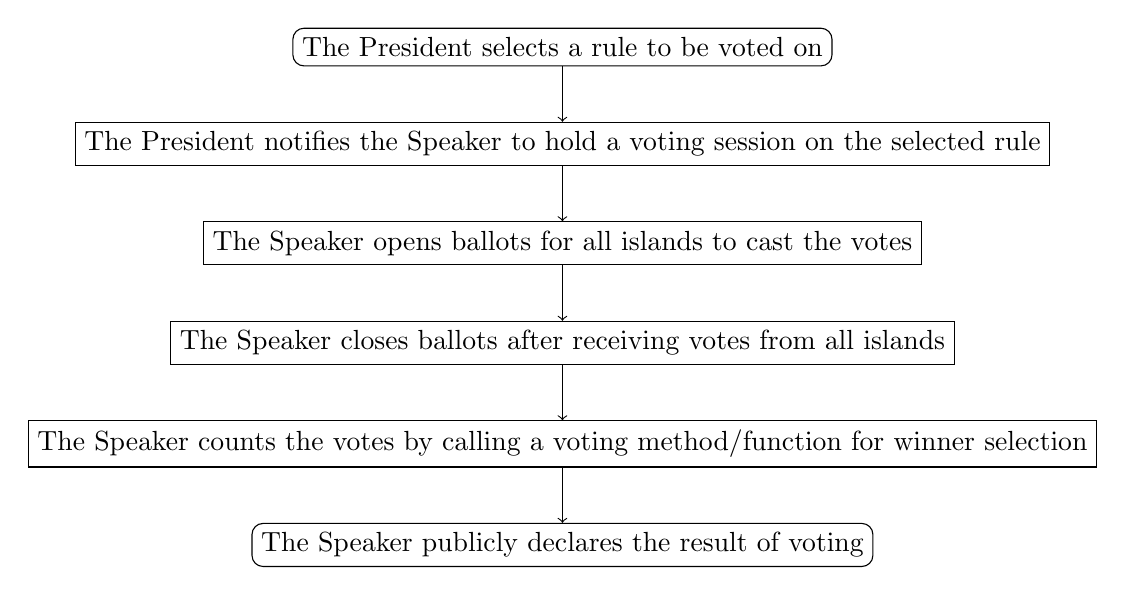
\begin{tikzpicture}[node distance=20pt]
\centering
\node[draw, rounded corners] (start)  {The President selects a rule to be voted on};
\node[draw, below=of start] (step 1)  {The President notifies the Speaker to hold a voting session on the selected rule};
\node[draw, below=of step 1] (step 2)  {The Speaker opens ballots for all islands to cast the votes};
\node[draw, below=of step 2] (step 3)  {The Speaker closes ballots after receiving votes from all islands};
\node[draw, below=of step 3] (step 4)  {The Speaker counts the votes by calling a voting method/function for winner selection};
\node[draw, below=of step 4, rounded corners] (end)   {The Speaker publicly declares the result of voting};
 \draw[->] (start)  -- (step 1);
 \draw[->] (step 1) -- (step 2);
 \draw[->] (step 2) -- (step 3);
 \draw[->] (step 3) -- (step 4);
 \draw[->] (step 4) -- (end);
\end{tikzpicture}
\caption{Voting Protocol for Rules}
\label{fig:RONRVotingProtocol}
\end{center}
\end{figure}

For elections of roles, the sequence of actions of the voting protocol is mostly similar to the above explanation in principle, except for some parameters, such as the motion of the vote which is the role itself (President, or Speaker, or Judge), the facilitator of the election/vote event which depends on what role is being held for election (refer to Chapter 5 IIGO for more details on change of roles and power transfer), and the applicable voting method function to call for election that will produce the result, which is different from the voting method used for rules. Refer to Section~\ref{sec:VotingMethods} for more details on voting methods to be used for elections of roles.

In the initial implementation, it is assumed that all 6 islands have the power to vote at any necessary voting scenario and no sanction or power restriction applied to any island when it comes to the right to vote. However, in the final implementation, some complications or dilemma are applied to, i.e. an/some island(s) could lose their right to vote or not permitted to participate in a voting event due to diplomatic sanction. Refer to Chapter 5 IIGO for details on diplomatic sanction. In this case, the Speaker will check and open the ballots to only eligible islands that have the right to vote at that certain stage, rather than to all islands as mentioned in the first scenario above.

\section{Implementation}
\label{sec:Implementation}

\subsection{Voting for Rules}
\label{sec:VotingForRules}
The implementation of voting for rules from infrastructure point of view (file:\texttt{rulevote.go}) basically follows the sequence of voting protocol as described in Section~\ref{sec:VotingProtocol}. At initialisation, there are two defined structs (collection of data fields) that are used as parameters for functions inside the voting algorithm, such as \texttt{RuleVote} and \texttt{BallotBox}. The \texttt{RuleVote} struct consists of 3 variables, i.e. \texttt{ruleToVote} (string) that contains the rule that has been selected by the President to be voted on, \texttt{islandsToVote} (list of integers) that contains a list of \texttt{ClientID} which indicates all eligible islands that participate in the voting session, and \texttt{ballots} (list of boolean) that contains the vote of each respective eligible islands where it can indicate the vote for in-favour or against the proposed rule. The \texttt{BallotBox} struct consists of 2 integer variables that act as accumulators for the count of each possible vote: \texttt{VotesInFavour} and \texttt{VotesAgainst}.

According to Section~\ref{sec:VotingProtocol}, The Speaker firstly starts a voting session by calling \texttt{SetRule(rule)} function that contains the rule selected by The President to be voted on. Next, the Speaker sets all eligible islands that can participate/have the right to vote in the voting session at that state of the game by using \texttt{SetVotingIslands(clientIDs[])} function. After that, the Speaker opens the ballots to get the votes from all eligible islands by calling \texttt{GatherBallots(clientMap[ClientID])} function. Subsequently, the \texttt{GetBallotBox()} function is called by the Speaker to gather the ballots that already contain the votes counting of those who are in-favour or against the proposed rule. Finally, the votes counting is concluded by comparing the votes of those in-favour vs those against, and the in-favour votes win when the counting is greater than or equal to the against votes counting, as reflected in \texttt{CountVotesMajority()} function. The Speaker then uses this result to declare the result of this voting session in IIGO.

\subsection{Elections}
\label{subsec:Elections}
The elections for roles implementation can be seen in the file:\texttt{election.go}. At initialisation, there is a defined struct \texttt{Election} that contains 4 parameters, i.e. \texttt{roleToElect} that indicates which role is being voted on (President, or Speaker, or Judge), \texttt{votingMethod} that indicates the voting method being used for the election to determine the winner selection, \texttt{islandsToVote} that contains a list of \texttt{ClientID} which indicates all eligible islands that participate in the voting session, and \texttt{votes} that is a list that contains the order rank of preference of the candidates for the role from each eligible island who casts the vote.

The election session begins by calling the \texttt{ProposeElection(role,method)} function that depends on which role being voted on and which role has obligation to facilitate the election (refer to Chapter 5 IIGO on Change of Roles and Power Transfer sections), and the selected voting method to be used for this election (refer to Section~\ref{sec:VotingMethods} for details on voting methods and Subsection~\ref{subsec:VotingPseudo} for pseudo-code implementation). The election facilitator then opens ballots to all eligible islands to cast their votes by calling \texttt{OpenBallot(clientIDs[])} function. The \texttt{Vote(clientMap[ClientID])} function gathers all the ballots containing the votes from all eligible islands that are obtained from \texttt{GetVoteForElection(roleToElect)} function returned from each client/island code execution. After that, the election facilitator closes the ballots by using \texttt{CloseBallot()} function and it returns the result of the votes counting using the selected voting method by calling each respective voting method function. This result is used by the election facilitator to declare the winner for the elected role. By default, the voting method for election is Borda Count and the function is called \texttt{bordaCountResult()} where the algorithm follows through what are explained in Section~\ref{sec:VotingMethods} and Subsection~\ref{subsec:VotingPseudo} where the Borda scores will be calculated based on the order rank of preference of the candidates from each ballot. The other voting methods can be used for election and it is selected by the election facilitator.

\subsection{Voting Methods Implementation Pseudo-code}
\label{subsec:VotingPseudo}

\textbf{Plurality}
\newline
Call for Voting inputs (int:IslandID, str:"Aye", "Nay" or "Abstain")\\
\begin{algorithm}[H]
\ForEach{$ballot \in ballots $}{
    \If{$Aye$} {Count for $Aye ++ $}
    \If{$Nay$} {Count for $Nay ++ $}
}
\If{$Aye > Nay$}{\Return the Winner: $Aye$}
\Else{\Return the Winner: $Nay$}
\end{algorithm}

\ \newline \ \newline \ \newline
\textbf{Borda Count}
\newline
\begin{algorithm}[H]
\For{all ballot}{
    $numNotIn\gets N-ballot.length$\\
    $shareScore\gets 1+...+numNotIn$\\
    \For{i from 0 to N-1}{
    \If{i is in ballots} {$scores[i]\gets scores[i]+N-K+1$ }
    \Else {$scores[i]\gets scores[i]+shareScore/numsNotIn$ }
    }
}
Sort candidates by Borda scores\\
\Return the candidate with the highest score
\end{algorithm}

\ \newline \ \newline \ \newline
\textbf{Runoff}
\newline
\begin{algorithm}[H]
\For{All $ballot \in ballots $}{
    Select two candidates with most first-placed votes
}
\If{either already has a majority}{
\Return the majority one}
\Else{Each voter selects one candidate of the top 2\\
}
\Return the candidate with the most votes
\end{algorithm}

\ \newline \ \newline \ \newline
\textbf{Instant Runoff}
\newline
\begin{algorithm}[H]
\ForEach{$ballot \in ballots $}{
\For{i from 0 to N-1}{
\If{i is first choice}{$scores[i]\gets scores[i]+N-K+1$}
}
}
\If{candidate in ballots $>1$}{
Remove the candidate with the fewest first
choice votes from the ballots.\\
GOTO the top for next round of counting
}
\Else{\Return the candidate}
\end{algorithm} 

\ \newline \ \newline \ \newline
\textbf{Approval}\\
\begin{algorithm}[H]
\ForEach{$ballot \in ballots $}{
    \For{i from 0 to N-1}{
    \If{i is in ballot} {$scores[i]\gets scores[i]+1$ }
    }

}
Sort candidates by scores\\
\Return the candidate with highest score
\end{algorithm}

    \chapter{Team 1 Agent Design}

\section{Core Idea}
Team 1 Agent was designed around the idea that the agent wants the whole archipelago to survive. However, the agent does have different configurations that allows it to be more malicious than intended such that interesting simulations may occur.

\section{Opinions on Islands}
For an agent to become self-organising, the agent must determine certain actions given a condition without external input. For this to be possible, the agent must have defined conditions which team 1 calls 'emotional state', and hold an opinion about other islands. This will form a basis for the agent to decide on an action.

Initially, the opinion on all existing islands are neutral. Overtime through IITO and IIGO, the opinions on islands will change. This will affect the outcome of IITO and IIGO results. As a note, positive values correspond to positive opinions while negative values correspond to negative opinions.

An agent's emotional state can change depending on the current resources. Below is an example of how an agent's emotional state can be formed:
\begin{itemize}
    \item If current resources > 10 * living cost, the agent is happy.
    \item If 3 * living cost < current resources < 10 * living cost, the agent is anxious.
    \item If the current resources < 3 * living cost, the agent is desperate.
\end{itemize}
The upper and lower bounds can be changed before a game starts. 

\section{IITO Gifts}
During IITO, the agent's opinion of other island is affected. For every gift received, the agent's opinion of the gifter increases. However, the agent's opinion of an island can decrease if that island promised a gift and was not able to fulfil it. 

When team 1 agent receives a request for gifts, the agent will decide how much to offer depending on the agent's current emotional state and the opinion of that island. 

\begin{table} [htb]
    \centering
    \begin{tabular}{|c|p{0.5\textwidth}|}
        \hline
        Emotional State & How is IITO handled? \\
        \hline
        Happy & Agent will give away its resources that satisfies the requested amount. \\
        \hline
        Anxious & Agent will give away a ratio of the requested amount and its current resources. \\
        \hline
        Desperate & Agent will refuse any gift requests that it receives. \\ 
        \hline
    \end{tabular}
\end{table}

Moreover, if the agent's opinion of an island is very high, the agent can decide to give gifts disregarding the agent's own anxiety. On the other hand, if an opinion of an island is very low, the agent can decide to refuse to send a gift even though the agent is happy. 

For increase survivability, team 1 agent will accept any gift offers that it receives. 

\subsection{Future Works}
Team 1 agent currently has a very straight-forward IITO strategy. Some interesting alteration to this strategy could include:
\begin{itemize}
    \item Being less suspectible to bribery. The agent should stop increasing the opinion of an island after receiving $X$ amount of continuous gifts.
    \item Stop handing out gifts to islands that are not in critical state.
    \item Being proactive in bribery. The agent will give unrequested gifts to the current president in hopes that this will reduce tax and increase resource allocation from the common pool. 
\end{itemize}

\section{IIFO Disaster Prediction}
Disasters can happen deterministically or stochastically (mentioned in detail in Chapter~\ref{sec: Disaster} for more information). For an agent, it is important to determine when a disaster occurs so that as much disaster damage is mitigated using the common pool. 

When the game starts, the disaster prediction made by the agent is random. This prediction always has a confidence value of 0. As more disasters occur, a history of disasters is built up. Using this history, the mean disaster position x, position y, magnitude and occurrence is calculated. A confidence value is calculated along with the mean disaster metrics. 

% Add a footnote on website?  https://www.mathsisfun.com/data/confidence-interval.html
The confidence value is calculated by finding the ratio between margin of error and the mean value. The smaller the margin of error, the more confident the agent is. Therefore, a difference between the mean value and the margin of error must also be calculated. To begin with, the agent uses the confidence interval equation (where $s =$ standard deviation, $n = $ size of array, $Z = $ confidence interval) to calculate the margin of error:
\begin{equation}
    \label{eq: Team1MarginOfError}
    \text{Error} = Z \dfrac{s}{\sqrt{n}} 
\end{equation}
Using the difference between the mean value ($\bar{x}$) and the margin of error along with finding out the ratio of this result will provide the agent with the confidence value.
\begin{equation}
    \text{Confidence Value} = (\bar{x} - \text{Error}) \times \dfrac{1}{\bar{x}}
\end{equation}

Sharing and obtaining other disaster information to and from other islands respectively can increase the survivability of the archipelago. As more disaster prediction is shared, a network of trust between team 1 agent and other island is built. This trust value is primarily based upon the absolute value of the islands prediction on the day the disaster happened. However, if an island shares a disaster prediction with the estimated disaster day to be random or changing erratically each turn, then team 1 agent will begin to distrust that island. 

\section{IIGO: President}

\section{Foraging}
Multiple foraging strategies were developed: 
\begin{itemize}
    \item Return on Investment (ROI)
    \item Regression
    \item Flip Forage
\end{itemize}

\subsection{Simulations against ourselves}

Multiple foraging strategies were developed, initially by intuition and later by attempting to address the shortcomings of previous attempts:

\subsection{Return on Investment (ROI) Foraging}%
\label{sec:forage-roi}

This first algorithm is based on repeating successful foraging behaviours in the past, whether those be by the agent herself or another agent.

For the first few turns (the exact amount is configurable) the agent will forage randomly.

The agent maintains a history of foraging decisions and outcomes, including those received from IIFO.\@ When it comes time to forage this history is sorted by ROI, i.e.\ the ratio of profit to contribution. Decisions that resulted in a loss, had profit smaller that the living cost, or had a larger contribution that a (configurable) percentage of available resources are filtered out.

\subsection{Regression Foraging}%
\label{sec:forage-regression}

This strategy tries to predict the ideal foraging decision, even if that exact decision was not made in the past. This is done using regression, which is used to find the decision with the highest expected reward.

% In detail, history is kept as in \nameref{sec:forage-roi}. To make a foraging decision, the history is split by foraged resource (fish or deer), and quadratic regression is performed on contribution versus reward. The maximum of the regression curve is found for each group and the contribution with the highest

\subsection{Flip Foraging}

This strategy chooses the least foraged resource from the last turn, according to IIFO-reported data. Contributed amount is proportional to the chosen resource's total ROI from last turn. This choice was made under the assumption that ROI is an indicator of the resource's ``condition''. If a resource only gives moderate rewards (proportionally to input) it means that it is probably over-used currently and as such agents should allow it to recover, by scaling down their foraging attempts.

\subsection{Comparison}

To compare the three strategies, simulations were run with six agents, two using \emph{ROI foraging}, two using \emph{regression foraging}, and two using \emph{flip foraging}. IIGO and IITO were also disabled in order to isolate the efficacy of foraging methods from other parts of the game. The simulation was run five times and the results averaged over the 5 games as well as the two agents following the same strategy.

\begin{figure}[H] 
\centering
\includegraphics[width=0.6\textwidth]{09_team1_agentdesign/images/mean_survival_turns}
\caption{Mean survival turns for different strategies.}
\label{fig:team1:mean_survival}
\end{figure} 

\begin{figure}[H] 
\centering
\includegraphics[width=0.6\textwidth]{09_team1_agentdesign/images/total_efficiency}
\caption{Average foraging efficiency}
\label{fig:team1:average_efficiency}
\end{figure} 

It is clear from \autoref{fig:team1:mean_survival} that the \emph{flip} foraging strategy dominates the other two in terms of overall effectiveness. However, it is interesting to note that, according to \autoref{fig:team1:average_efficiency}, the \emph{ROI} foraging method is almost as efficient as \emph{flip}, which raises the question of what causes the difference in their success. This difference could be attributed to one core issue with the \emph{ROI strategy}: ignoring the absolute value of rewards. The agent will happily settle for a profit of $11$ resources, if that was obtained with a contribution of $0.1$ resources (a profit of $110000\%$) over a profit $50$ resources for a contribution of $25$ (a measly $100\%$). This means that in the long run living costs overwhelm the \emph{ROI} agent. The \emph{flip} agent does not take expected profit into account and as such is unaffected by this.

\emph{Regression} appears to occupy a medium between \emph{flip} and \emph{ROI}, however it is much less consistent, as evidenced by the error bars in \autoref{fig:team1:mean_survival}, with \emph{regression} surviving for under 10 turns in some runs.

%%% Local Variables:
%%% mode: latex
%%% TeX-master: "../main"
%%% End:

    \chapter{Team 2 Agent Design}
\section{Overall Agent Strategy}

The overall strategy of our agent is based on a series of distinct, overlapping dilemmas. The agent operates on principles based on Evolutionary Economic Theory \footnote{https://www.cambridge.org/core/what-we-publish/elements/evolutionary-economics}. Game theory and the use of the Nash equilibrium also guided the development of the strategies implemented. The other top-level strategy which overlaps with several dilemmas is the social dilemma; this is when we quantify the relationship we have with other agents to produce trust and confidence levels. The interaction between the top-level strategies with all of the dilemmas is shown in Figure~\ref{fig: top level strategy}. The top-level strategy's implementation into each agent function and role is discussed in the following sections. 

\begin{figure}[!htb]
    \centering
    \begin{subfigure}{.49\textwidth}
        \centering
        \includegraphics[width=0.99\textwidth]{images/strategies.png}
        \caption{Top level strategy}
        \label{fig: top level strategy}    
    \end{subfigure}
    \begin{subfigure}{.49\textwidth}
        \centering
        \includegraphics[width=0.9\textwidth]{images/dichotomy.png}
        \caption{Ceremonial-Instrumental dichotomy}
        \label{fig: dichotomy}
    \end{subfigure}
\end{figure}

\subsection{Evolutionary Economic Theory}
The term Evolutionary Economic Theory was first coined by economist Thorstein Veblen \footnote{https://www.cambridge.org/core/what-we-publish/elements/evolutionary-economics}. Evolutionary Economic Theory proposes that economic processes evolve, and it rejects the assumptions of classical rational choice theory. From Evolutionary Economic Theory, we categorised agent behaviour into distinct groups \footnote{https://www.cambridge.org/core/what-we-publish/elements/evolutionary-economics}. These groups are an altruist, fair sharer, and free rider. These are explained in Table~\ref{tab:Evolutionary Economic Theory Agent classifications}.

\begin{table}[!htb]
\caption{Evolutionary Economic Theory Agent classifications}
\label{tab:Evolutionary Economic Theory Agent classifications}
\begin{tabular}{|c|c|l|}
\hline
\textbf{Agent classification} & \textbf{Definition}                                                                                                                        & \multicolumn{1}{c|}{\textbf{Examples within the game}}                                                                                                        \\ \hline
Altruist                      & \begin{tabular}[c]{@{}c@{}}More concerned about the welfare \\ of the group than themselves\end{tabular}                                   & \begin{tabular}[c]{@{}l@{}}-Contributes a surplus to the common pool\\ -Generous with gifts\end{tabular}                                                     \\ \hline
Fair Sharer                   & \begin{tabular}[c]{@{}c@{}}Contributes enough to the group \\ to negate their negative impact on it\end{tabular}                           & \begin{tabular}[c]{@{}l@{}}-Contributes the minimum necessary amount of resources \\ -Gift allocation is measured and reasonable\end{tabular}                          \\ \hline
Free rider                    & \multicolumn{1}{l|}{\begin{tabular}[c]{@{}l@{}}More concerned with their individual \\ welfare than the welfare of the group\end{tabular}} & \begin{tabular}[c]{@{}l@{}}-Will not contribute enough to the common pool \\ -Gift requests above their requirement \\ -Will not give out gifts\end{tabular} \\ \hline
\end{tabular}
\end{table}

The advantage of using this theory over rational choice theory from classical economics is that it accounts for the irrational decisions agents or humans make when dealing with economic decisions, such as deciding how much to contribute to a common pool. Humans have evolved to develop heuristics \footnote{https://www.sciencedirect.com/topics/social-sciences/heuristics} which are "rules of thumb" in order to make economic decisions quickly and when all information is not present. These heuristics are typically based on emotion and will often result in irrational decisions; an example of this would be brand loyalty. This is very relevant within the context of the game because there is a cost to large computations (decision making). Also, there is an information failure \footnote{https://www.economicsonline.co.uk/Market_failures/Information_failure.html} as the agents often do not know the threshold of the common pool and other vital game metrics. This information failure forces agents to use heuristics similar to those used by real people. An excellent example of a heuristic within this agent strategy is the level of trustworthiness decided within the social dilemma. If every agent was rational and all information was present in the game, there is no need to trust or distrust agents as they would maximize both their welfare and that of others.

Another primary reason for selecting this theory as the basis of our design is to explore the ceremonial-instrumental dichotomy\footnote{https://www.jstor.org/stable/3486187?seq=3#metadata_info_tab_contents}. This dichotomy is best represented by the graph in figure \ref{fig: dichotomy} and shows the importance of the game's setup. Our agent is attempting to oppose this traditional response to instrumental and ceremonial societies. It would be interesting to change the game's ceremonial and instrumental values by changing the setup. While the current game infrastructure does not support this, it would be interesting to investigate the ceremonial-instrumental dichotomy by allowing islands to invest resources into developing their foraging technology to obtain higher returns. It would be interesting to investigate how this instrumental shift would change our agent's strategy and others' actions. This update in technology would replace the ceremonial institutional set up of the IIGO as it becomes redundant. Allowing islands to invest in technological advancement would add an extra dimension to the game as it evolves, and the importance of the IIGO and other instrumental components would shift.

\subsection{Evolutionary Economic Theory Implementation}
%explain how we use the information from the theory

Figure~\ref{fig:methods-of-play} shows the different states of our agent's different methods of play. At any point during the game, the state of our agent is determined only by the level of the Common Pool. Our agent's objective is to oppose the strategies employed by other agents to attain stability in the game. To determine the method of play of the other agents, we look at whether the Common Pool is, on average, increasing or decreasing. If the pool is being depleted, it can be assumed that the other agents act as free-riders on average. To counteract this, we act as an altruist (see section \ref{sec:Common Pool Dilemma Strategy} for more detail). The average pool level is used because individual agent strategies are irrelevant for the game's overall course. Within the game, we also do not always have access to individual agents' contributions, which would be needed to classify them individually. This makes the average level of the Common Pool the only viable parameter. 

Our simulations demonstrated that starting the game in a "free-rider" state resulted in optimal agent performance and did not negatively impact the course of the game overall.

The default state for the agent is to be a "fair sharer." The agent will move into altruist mode when the weighted average of the Common Pool has dropped drastically. The agent considers a weighted average to ensure that the agent does not panic after every disaster and over contribute. The most recent turns will also be weighed higher to determine the course of the game. When the Common Pool stops decreasing, the agent will move back to fair sharer mode. Similarly, if the pool's weighted average increases by a large factor, then our agent moves into a free-rider state.

\begin{figure}
\centering
\begin{subfigure}{.49\textwidth}
    \centering
    \includegraphics[width=0.9\textwidth]{images/MethodofPlay.png}
    \caption{Method of Play diagram}
    \label{fig:methods-of-play}
\end{subfigure}
\begin{subfigure}{.49\textwidth}
    \centering
    \includegraphics[width=0.9\textwidth]{images/Social.png}
    \caption{Social Classification Order}
    \label{fig:social-order}
\end{subfigure}
\end{figure}

\subsection{Social Classification}
The agent forms an opinion on others depending on different situations. Initial testing suggested that another island's gift-giving behaviour does not necessarily correlate with their quality of predictions. Consequently, the trust of other agents is computed and stored separately for each situation. The agent uses the weighted average of past interactions with other agents to determine whether or not to trust them in each situation for future interactions. Using a weighted average to compute trust resulted in notably better agent performance. This is because the agent's trust in other agents considers all interactions with other agents while weighting recent interactions more heavily.

An integer value represents the agent's trust metric for each agent in each situation between 0 and 100, where 100 denotes full confidence and 0 a complete lack thereof. This value is used to compute the expected outcomes of situations. These are then compared with real events to update the agent's confidence in the other agents regarding this situation. For example, when the agent receives predictions from other islands, it computes the weighted average to check whether it trusts the island. Once a disaster occurs, the magnitude or timing of the disaster is compared with the other island's prediction. This reality is used to assess their behaviour and update the trust metric for that island relating to that situation. The list of different "situations" includes how an agent behaves in a role such as the President, Judge, Speaker, gift-giving, and disaster prediction. The overall structure of how the agent forms opinions on other islands is shown in Figure~\ref{fig:social-order}.

\section{Gift Giving and Receiving}
The agent must decide whether or not to respond to other agents' gift requests and how much to request from others through gifting. The implementation does not consider whether or not an agent is critical when requesting gifts and instead considers its current method of play and the trustworthiness of the requesting agent. Figure~\ref{fig: gifts} shows a decision tree for how the agent will allocate or request gifts, in which the agent splits up the gift request among the other agents to increase the likelihood of an agent allocating the gift.


\begin{figure}[!htb]
    \begin{subfigure}{.49\textwidth}
        \centering
        \includegraphics[width=0.99\textwidth]{images/gifts.png}
        \caption{Gift Giving and Receiving decision tree}
        \label{fig: gifts}
    \end{subfigure}
    \begin{subfigure}{.49\textwidth}
        \centering
        \includegraphics[width=0.99\textwidth]{images/common_pool_strategy.png}
        \caption{Common Pool Strategy}
        \label{fig: common_pool_strategy}        
    \end{subfigure}
\end{figure}

Depending on the method of play, the agent will request more or fewer gifts. This is inversely proportional to the number of resources taken from the Common Pool. The agent obtains a larger proportion of its needed resources from gifting than the Common Pool in the altruist state. This is done to mitigate common pool depletion in the interest of the common good. In a Fair-Sharer state, the agent aims to obtain its resource target equally from gifts and the Common Pool. A minor surplus is also included in the resource target to ensure that the goal is met, given that gifts from other agents cannot be guaranteed. In a Free-Rider state, the agent takes the majority of its resources directly from the Common Pool but still requests gifts to build up its resources by taking advantage of relationships with other agents as well as a Common Pool surplus.

The \textbf{Gifts} social classification situation refers to both when an island requests a gift from our agent and when our agent requests a gift from that island. The balance between agent gift requests and responses is used as a basis for opinion formation on another agent. Other agents that fulfill the agent's requests are rewarded with higher trust. The agent's own gift requests tend to be small but are also proportional to its trust in each other agent. Every gift interaction is used to update the agent's trust in another island's gifting behaviour.

\section{Common Pool Dilemma Strategy} \label{sec:Common Pool Dilemma Strategy}
The Common Pool dilemma strategy can be split into two considerations. One consideration is the current method of play (altruist, fair sharer, and free-rider), and the other is the current game state. A decision tree showing the common pool strategy is shown in Figure~\ref{fig: common_pool_strategy}. These considerations decide whether and how much we contribute or take from the Common Pool.

\subsection{Method of play consideration} \label{ssec:Method of play consideration}
The primary consideration for giving to the Common Pool dilemma is the agent's current method of play. The agent's state is determined by the Common Pool level, as seen in Figure~\ref{fig:methods-of-play}. The agent's default state as a "fair sharer" contributes the average amount of other agents to the Common Pool. This is calculated by evaluating changes in the Common Pool level from the previous turn and averaging this quantity by dividing by the number of alive agents. If the Common Pool level decreases, the most recent Common pool increase is used to determine the amount given.

By using the average Common Pool contribution, the agent benefits from the forecasting of other agents. This benefit would arise should another agent have an advanced forecasting prediction that determines the Common Pool threshold and what is required to mitigate the effects of a disaster. In this case, the agent would then contribute a similar quantity of resources. This "herd-mentality" approach relies on the assumption that other agents make rational decisions. So if it is evident that other agents are acting irrationally, the agent deviates from this approach to an alternative state (to become either a free-rider or an altruist).

The agent is in an altruist state when the Common Pool is struggling, which often means that other agents act as free-riders. This is where the meta-strategy of Evolutionary Economic Theory comes into play. It is in the agent's interest to contribute much more to the Common Pool to alter the game's course in a positive direction and prevent the pool from being below the threshold when a disaster occurs. Therefore, the agent contributes more resources to enact this balance on the system. 
The altruist resource contribution is a larger factor of the weighted average contribution and can be tuned using the \emph{altruist factor} variable in the agent's configuration.

In a free-rider state, the Common Pool has a surplus, and the agent assumes other agents are on average operating as altruists. In this situation, the agent contributes less to the Common Pool and preserves resources to mitigate short and long-term risk. Contributing too much to the Common Pool no longer benefits the greater good, as these resources can still be used to forage and generate more resources. Therefore, the agent accumulates resources when others are too generous, allowing greater foraging investments and making it easier to help other agents if they struggle in the future.

The method of play also impacts how the agent decides to take from the Common Pool. After game state considerations are made, the agent adjusts how much it takes from the Common Pool according to its Agent State. Table~\ref{tab:Method of play common pool taking} outlines a summary of how the agent adjusts how much it takes and gives a justification for each action. The amount to take from the pool depends on how willing other agents are to contribute to the agent within the game's gift-giving section.  This means the agent must decide what proportion of the resource request must be taken from the Common Pool and from gifting, and this decision also factors in both common pool allocation as well as gift response predictions. When the agent is in a free-rider state, the common pool has a surplus, and so it makes more sense to take directly from the pool rather than requesting gifts. 

\begin{table}[!htb]
\centering
\caption{Method of play common pool taking}
\label{tab:Method of play common pool taking}
\begin{tabular}{|c|c|}
\hline
\textbf{Agent classification} & \textbf{How this impacts taking from the common pool}                              \\ \hline
Altruist                      & Pool is being depleted, best to not take from the pool                             \\ \hline
Fair Sharer                   & Gift requests and taking from the pool are equal                                   \\ \hline
Free rider                    & \multicolumn{1}{l|}{Pool has surplus, take from the pool rather than gift request} \\ \hline
\end{tabular}
\end{table}

\subsection{Game state consideration} \label{ssec:Game state consideration}
The primary consideration in taking from the Common Pool is the current game state. The key parameters (shown in Figure~\ref{fig: common_pool_strategy}) considered are whether the agent is critical and whether the agent has excess resources. This excess is calculated as the difference between the agent's current resources and the minimum resource threshold and the cost of living. Beyond this minimum resource level, the agent can survive one another turn. If the agent has fewer resources than these aggregated costs, the excess is zero. If there are excess resources, the agent will give some resources to the Common Pool. In this case, a strategic contribution is calculated. If the Common Pool threshold is known, the agent considers how many resources are required to attain this threshold. This is then spread over the expected number of turns until the next disaster is predicted to occur and the number of alive clients. If this is unknown, a default value is used to form an initial guess in the agent configuration. On top of this quantity, a strategic contribution is also calculated (see \ref{ssec:Method of play consideration}). The current method of play determines whether the disaster-determined contribution or the strategy-determined contribution is contributed to the pool. This amount is then contributed together with the current tax, unless there are no excess resources as this implies the agent is in a critical state and so all resources are preserved.

\section{Foraging Dilemma}
The foraging dilemma is split into two parts. One determines whether the agent should hunt or fish, and the other determines how many resources to spend on foraging. The foraging dilemma only depends on the current method of play. The method of play will impact the amount the agent uses to forages. If the Common Pool is doing well and the agent acts as a free rider, it will be more prone to take risk and contribute more to the foraging and vice versa. The decision to hunt or fish depends on the likely number of hunters in the next foraging event. The decision tree, Figure~\ref{fig: Hunt or fish decision tree }, shows how the agent decides whether to hunt or fish in a given turn. To determine the number of hunters in the next forage turn, the agent tracks how often each agent is a hunter and then sums up the probability of each agent hunting to find an overall number of likely hunters. The agent outputs a random number from 0 to 1, and if the number lies above the threshold, the agent will hunt. This threshold is determined by the number of likely hunters in the foraging. It implies there is an element of randomness to the agent's decision making, which will account for the unpredictability of dealing with other agents with their strategies.

\begin{figure}[!htb]
    \centering
    \begin{subfigure}{.49\textwidth}
        \centering
        \includegraphics[width=0.9\textwidth]{images/forage_decision.png}
        \caption{Hunt or fish decision tree }
        \label{fig: Hunt or fish decision tree }
    \end{subfigure}
    \begin{subfigure}{.49\textwidth}
        \centering
        \includegraphics[width=1.0\textwidth]{images/Roles Decision Tree.png}
        \caption{Roles Decision Tree}
        \label{fig: Roles Decision Tree}        
    \end{subfigure}
    \caption{Hunting or Fishing and Roles Decision Tree}
\end{figure}

The ideal distribution for foraging is to have two agents hunting and the remainder fishing. Hence, when the agent predicts one other agent will hunt, the agent is highly likely to choose to hunt too. The default threshold for hunting is 0.1, so the agent will hunt 10\% of the time when not considering the likely number of hunters. By assuming that any agent will hunt or fish with equal probability, the likelihood that there is one hunter is approximately 0.16. This implies hunting is an optimal strategy approximately 16\% of the time, so a threshold similar to this value is chosen. If the predicted number of hunters is above one, the following equation is used to determine threshold placement: $\text{Probability of agent hunting} = 0.95 - \text{Predicted number of hunters} \times 0.15$

The probability of choosing to hunt when the agent is confident only one other agent will also select hunt is 0.95. For each additionally predicted hunter, the probability will fall by 0.15. This 0.95 threshold is included in the agent configuration so it can be edited without changing the code. Hence, the foraging decision can be tuned. The agent checks if there are any excess resources after considering the minimum resource threshold not to be critical and the cost of living. If there are no excess resources, no resources are spent on foraging. If there is an excess of resources, a percentage of this excess is used on foraging. This percentage is controlled in the agent configuration. This approach ensures the agent has enough resources to survive another round, even in the worst case scenario when foraging returns are minimal.

\section{Role Strategies}

Figure~\ref{fig: Roles Decision Tree} shows a decision tree of how the agent acts under the two roles implemented. Due to time constraints, the base client implementation was used for the Speaker. The President is responsible for allocating resources from the Common Pool based on agent requests. The agent uses game state variables such as their critical status to determine if another agent is worthy of their resource request and the agent's allocation method based on the method of play is outlined in Table~\ref{tab:President allocation method of play}. When the agent is in a free-rider state, it is more selfish, while when it is an altruist, more of the others agents requests are approved. If an agent is not critical, it is highly unlikely that the agent will allocate them their requested resources as the purpose of the Common Pool should be to primarily mitigate the effects of disasters. Resources are allocated on a need-first basis, taxed proportionally to an agents resource level, and the strategy to determine taxation includes an additional penalty tax for agents who do not declare their resource levels. When evaluating another President's performance, the agent considers the percentage change in tax, the percentage of how much the agent is allocated with respect to how much it requests, and how much the agent takes with respect to how much the President allocates it.

\begin{table}[!htb]
\centering
\caption{President allocation method of play}
\label{tab:President allocation method of play}
\begin{tabular}{|c|c|}
\hline
\textbf{Agent classification} & \textbf{\% of request given} \\ \hline
Altruist                      & 60                           \\ \hline
Fair Sharer                   & 50                           \\ \hline
Free rider                    & 40                           \\ \hline
\end{tabular}
\end{table}

The agent implementation of the Judge evaluates whether an agent has broken any rules, as it should. However, to model real world corruption, the agent does not sanction agents that break rules if it considers them to be highly trustworthy (i.e., with a trust score above 80\%). The agents behaviour as a Judge is also determined by its state; when the agent is a free-rider, it sanctions fewer islands. The \textbf{Judge}'s situation, similar to the President, is used by the agent to determine what island to vote for as Judge. This is done by checking the past sanctions the agent received and their duration, to maxmimise personal benefit. The \textbf{RoleOpinion} social classification situation is used when the agent is the Judge and must decide whether or not to pardon other islands' sanctions, whom to choose as the next President whether or not an island has adhered by the rules. The Judge receives information for each island, such as the difference between how much an island contributed to the common pool and how much said they would. The agent uses these differences as a Judge to determine whether or not an island is trustworthy. During a role election, the agent checks its trust in the candidates for the appropriate situation, i.e., the situation when an agent is "President" for a future Presidential election. The agent will return a list of candidates in decreasing order of preference determined by the social classification. To do this, the agent sorts the candidates in terms of how much it trusts them.

\section{Disaster Prediction}
It is important for the agent to be capable of predicting both the severity and timing of disasters, in order to effectively make decisions for contributing to both the common pool and gifting resources to other agents.

Since the simulation is constructed through a series of successive turns, the occurrence of disasters throughout the game can be seen as a Binomial distribution: $D \sim \text{Bin}(n,p)$. In this equation, $D$ describes the number of disasters that occur, $n$ is the number of turns played and $p$ is the probability of a disaster occurring on a given turn.

The aim of our agent is to estimate the number of turns between disasters. We will denote this random variable as $T_D$, with our agent's aim being to find $E[T_D]$. To do this, our agent must estimate $p$. Therefore we have programmed our agent to find the Maximum Likelihood Estimator of $p$ for a Binomial RV\footnote{https://stats.stackexchange.com/questions/191444/variance-in-estimating-p-for-a-binomial-distribution}: $\hat{p} = \frac{D}{n} = \bar{X}$, where $\bar{X}$ is the sample mean of the RV $X$. The expectation of $T_D$ can be estimated using\footnote{https://math.stackexchange.com/questions/1299465/proof-variance-of-geometric-distribution}: $\hat{\mu}_{T_D}= \frac{1}{\hat{p}} = \frac{1}{\bar{X}}$. Thus, this is the optimal estimator for our agent to predict the number of turns between disasters. Furthermore, the confidence that our agent has in this prediction should be inversely proportional to the variance of $T_D$, i.e. how much does $T_D$ vary from the expected value we have found above? The expression for this variance is given below$^2$: $Var(T_D)= \frac{1-p}{p^2}$. 

However, given that our agent does not know the actual value of $p$ used in the simulation, our agent instead estimates the variance using: $\hat{\sigma}_{T_D}^2= \frac{1-\hat{p}}{\hat{p}^2}$. Now that an expression for the estimate of this variance has been obtained, two questions remain: ``what about the variance in $\hat{p}$" and ``how is this variance translated into a confidence value?" The variance of $\hat{p}$ is given by the following expression: $Var(\hat{p})= Var(\bar{X}) = \frac{Var(X)}{n}$. As previously, we do not know the exact value of $p$, making a calculation of $Var(X)$ impossible. However, we can make use of the fact that $Var(\hat{p}) \propto \frac{1}{n}$, by making our agents confidence in the prediction proportional to $n$ also. Secondly, the fact that variance can take values $\in [0,\infty]$ but confidence must take a value $\in [0, 100]$ makes mapping the values of variance that our agent calculates, to a confidence level, challenging. The solution our team opted for was to cap the max value of variance to some value $v_{cap_{T_D}}$, before translating this variance into a corresponding confidence value. This process is given by the equation below: $\text{confidence}_{T_D} = 100 - \frac{100 \cdot \text{min}(\frac{\hat{\sigma}_{T_D}^2}{kn}, v_{cap_{T_D}})}{v_{cap_{T_D}}}$ 
where $k$ is the tuning parameter for altering the dependence of the confidence on $n$. 

\subsection{Magnitude Prediction}
Our agent's strategy for predicting the magnitude of the next disaster shares many similarities with the strategy discussed in the last section. However, the magnitude of the next disaster is now distributed with an Exponential distribution: $M \sim Exp(\lambda)$. Once again, start by finding the MLE for the parameter $\lambda$ \footnote{https://en.wikipedia.org/wiki/Exponential\_distribution}: $\hat{\lambda} = \frac{1}{\bar{M}}$. Now we seek to estimate the expectation of $M$: $\hat{\mu}_M = \frac{1}{\hat{\lambda}} = \bar{M}$. Similarly, the variance of this RV is also useful to estimate $\hat{\sigma}_{M}^2= \frac{1}{\hat{\lambda}^2}$. As previously, there is also a variance in our estimation of $\hat{\lambda}$ that must be taken into account by making our confidence in this prediction proportional to $n$. Thus, the following expression should be used for calculating the confidence in the magnitude prediction: $\text{confidence}_M = 100 - \frac{100 \cdot \text{min}(\frac{\hat{\sigma}_{M}^2}{gn}, v_{cap_M})}{v_{cap_M}}$, where $g$ is the tuning parameter for altering the dependence of the confidence on $n$. 

\subsection{Overall Prediction}
The overall prediction that must be shared with teams during the IIFO session requires the following information: location, time until next disaster, magnitude and confidence. For our prediction of location, the middle of the archipelago is always given since the probability of a disaster occurring at a given location is uniform across the archipelago, meaning that there is no optimal prediction formula. Using the findings presented in the above sections, the formulas our agent will use to form a prediction about the next disaster are as follows:

\begin{align*}
    &x_{coord} = x_{min} + \frac{(x_{max}-x_{min})}{2}, y_{coord} = y_{min} + \frac{(y_{max}-y_{min})}{2}, \text{conf} =\frac{\text{conf}_{T_D} + \text{conf}_M}{2} \\
    &\hat{\mu}_{T_D}=\frac{1}{\bar{X}}, \hat{\mu}_M = \bar{M} \\
\end{align*}

\subsection{Combined Prediction}
Generating our own prediction is only the first part of the prediction making process. The second stage is to make use of other island's predictions during the IIFO session and using the social classification to decide prediction accuracy. When considering how much emphasis to put on a given island's prediction, we make use of two factors: 1.) Our island's confidence in each other island's prediction making. 2.) Each island's confidence in their own prediction, $P_i \in [0,100]$. These two considerations are then combined to create an overall confidence factor.

\section{Simulations}
Every function and agent consideration has tuneable parameter which can be edited without changing the whole agent. Figure~\ref{fig: Forage Untuned} shows how our agent reacts when it plays against itself and the foraging parameters are untuned. As you can see the game is unstable and the agents have a low survival rate. This is caused by an over contribution to the foraging dilemma, there is a point of marginal return with the foraging dilemma and spending too many resources can be wasteful. 

\begin{figure}[!htb]
    \centering
    \includegraphics[width=0.6\textwidth]{images/Forage Untuned.png}
    \caption{Untuned Forage Simulation}
    \label{fig: Forage Untuned}
\end{figure}

Figure~\ref{fig: Forage tuned} shows how our agents plays against itself when the foraging parameters are optimised. The amount of excess resources spent on foraging is more reasonable in this simulation, this results in a much higher survival rate and a more stable common pool.

\begin{figure}[!htb]
    \centering
    \includegraphics[width=0.6\textwidth]{images/Forage tuned.png}
    \caption{Tuned Forage Simulation}
    \label{fig: Forage tuned}
\end{figure}

Figure~\ref{fig: altruist sim}  shows what happens when the agent plays itself and they are all altruists by default and do not move out of altruist. It can be seen that the agents over contribute to the Common Pool and are left with nothing to forage, this ends the game rather quickly. The simulation result was very similar for when all of the agents were free riders, the game would end in a couple of rounds after a lack of contribution to the common pool which caused impactful disasters.  This proves that being a free rider or altruist is not a rational decision and must be avoided. 
%the other graph is not really as expected so lets just keep it like this

\begin{figure}[!htb]
    \centering
    \includegraphics[width=0.7\textwidth]{images/altruist sim.png}
    \caption{Altruist simulation}
    \label{fig:  altruist sim}
\end{figure}
     \documentclass{article}

\usepackage[legalpaper, potrait, margin=1in]{geometry}
\usepackage[utf8]{inputenc}
\usepackage{gensymb}
\usepackage{graphicx}
\usepackage{float}
\usepackage{color,soul}
\usepackage[dvipsnames]{xcolor}
\usepackage{float}
\usepackage{array}
\usepackage{arydshln}
\usepackage{amsthm}
\usepackage{adjustbox}
\newtheorem{definition}{Definition}
\setlength\dashlinedash{0.2pt}
\setlength\dashlinegap{1.5pt}
\setlength\arrayrulewidth{0.3pt}
 
 \usepackage[linesnumbered,ruled,vlined]{algorithm2e}


 
 

\newenvironment{conditions}
  {\par\vspace{\abovedisplayskip}\noindent\begin{tabular}{>{$}l<{$} @{${}={}$} l}}
  {\end{tabular}\par\vspace{\belowdisplayskip}}


\title{Team 3: Pittstop Agent Strategy}

\begin{document}

\maketitle

\section{Introduction}

Team 3 was interested in the parallels between this project and human societies. We wanted to build an agent that was flexible enough to mimic the diverse personality traits of ordinary citizens, as well leaders in governments around the world.

Section~\ref{sec:overall_strat} discusses the foundation of parameters and methods the team wrote in its approach towards building the agent. Section~\ref{section_func_team3} details how the team used this foundation to implement the required functionality of the agent (i.e. roles, voting, prediction, gifting, foraging) in a way that is compatible with our goal of flexibility, without compromising efficiency or intelligence. Section~\ref{sec:team3_simulation} then elaborates on game simulations, in which the team decided to anthropomorphize the agent by modelling it after three famous historical and political personalities. Simulations consisting of different permutations of these personalities reveal interesting conclusions about the performance of the archipelago. Finally, Section~\ref{sec:management} concludes our report with information about project management.

\section{Overall Agent Strategy}
\label{sec:overall_strat}

\subsection{Overview}
\label{sec:overview}


The agent was created by first a set of high-level parameters, most of which were used as scaling factors throughout the code base of the agent, and some as Boolean values that turn on or off specific behaviours. These parameters hence govern the agents interactions with the rest of the game. The effect of each parameter on the behaviour of the agent is summarized in Table~\ref{tab:team3:parameter_effects}. \\


\begin{center}
    
\begin{table}[H]
\centering
\begin{tabular}{l|l}
\textbf{Parameters} & \textbf{Description}  \\ 
\hline
\texttt{equity}                       & controls the allocation distribution of resources amongst islands              \\ \hdashline
\texttt{resourceSkew}                 & factor to adjust resource allocation based on trust             \\ \hdashline
\texttt{complianceLevel}              & quantifies how often the agent cheata during the game             \\ \hdashline
\texttt{saveCriticalIsland}           & if True, our agent will try to save any critical island             \\ \hdashline
\texttt{selfishness}                  & quantifies how selfish our agent is (e.g. in the context of gifts)             \\ \hdashline
\texttt{riskFactor}                   & quantifies how much risk our agent is willing to take        \\ \hdashline
\texttt{friendliness}                 & quantifies how friendly we will be during agent interactions            \\ \hdashline
\texttt{sensitivity}                  & quantifies how sensitive the agent will be to external changes            \\ \hdashline
\texttt{giftInflationPercentage}      & factor to adjust when gift requests are made to other islands             \\ \hdashline
\texttt{advType}                      & enables the agent to exploit institutional powers when elected in a role    \\ \hdashline
\texttt{controlLoop}                  & boolean to enable the feedback loop for the agent       
\end{tabular}
\caption{List of global parameters that dictate our agent strategy.}
\label{tab:team3:parameter_effects}
\end{table}
\end{center}

\subsection{Core functions}

Based on these parameters, we also wrote a set of core functions which would be useful to all variations of the agent. These functions implement Opinion Formation and Compliance Calculation.


\subsubsection*{Opinion Formation} \label{section_opinion_formation}
In a game where there can be up to n-agents, \textit{opinion formation} allows our agent to quantitatively assess the behaviour of the others based on previous interactions. %The agent uses this information in the form of \textit{trust decision-making} to reduce uncertainties and ultimately maximise its returns during any activity. 
In our implementation, we use a \texttt{trustScore} map to keep track of the agent's trust in (n-1)-agents. This map is used in combination with other pre-configured parameters to make strategic decisions during a turn. 
Trust takes a score between 0 (lowest) and 100 (highest). At the beginning of the game, all trust scores are initialised at 50, representing a neutral opinion. In our implementation, the trust scores can change during the following game activities:

\begin{itemize}
    \item Gifting: When our agent receives gift offers (after requesting gifts) and actual gift amount(s) received.
    \item Role Evaluations: When our agent evaluates the performance of the President, the Speaker and the Judge based on their respective roles and responsibilities.
    \item Sanctions: When we receive the broadcast of sanction from the Judge outlining the sanctions placed for that turn.
\end{itemize}

%This mean that the more turns there are in a game, the more variation one will observe in the trust scores. They provide an effective source of perceived opinion for the agent to intelligently devise and choose a strategy in a given situation with limited external information. 

At every turn of the game, the agent will participate in multiple activities and hence, it would be counter-intuitive if the agent directly updated the \texttt{trustScore} map otherwise only the last score change would be retained. We thus implemented a local cache, \texttt{trustMapAgg}, to keep track of all trust score updates made during agent activities for that turn. 

In the following turn, the \texttt{trustScore} map is updated by averaging all cached trust score changes for each agent in play. This allows the agent to progressively accumulate knowledge while still forming independent opinions from the results of the activities in each turn. Trust scores are also bounded between 0 and 100 for consistency. The process (for a single turn) is summarized in Figure~\ref{fig:trust_scores}.\\

\begin{figure}[H] 
\centering
\includegraphics[width=0.75\textwidth]{figures/TrustScores.jpg}
\caption{Diagram showing the series of changes to trust scores during a single turn.}
\label{fig:trust_scores}
\end{figure}

%The \texttt{trustScore}  For example, when our island is elected as a Judge, the agent will rely upon these trust scores to determine which islands to pardon. This allows the agent to facilitate trust and forgiveness within the same framework.

\subsubsection*{Compliance Calculation}
Compliance Calculation determines at what point of the game it is most strategic to cheat. At every turn we calculate the \texttt{compliance} for the next turn\footnote{Note that \texttt{compliance} is how much our agent should comply at a given turn, while \texttt{complianceLevel} is how much our agent should comply during the entire game.}. The compliance calculation is based on the following principles:
\begin{enumerate}
    \item Every time we are caught, \texttt{compliance} is reset to 1.
    \item The more our agent is caught, the less it should cheat.
    \item If our agent has not been caught cheating for an infinite amount of turns, $\texttt{compliance}=\texttt{complianceLevel}$.
    \item The more our agent is caught, the longer it should take \texttt{compliance} to converge to \texttt{complianceLevel}.
\end{enumerate}

Those principles were converted into Equation~\ref{team3:eq:compliance}, shown here below:

\begin{equation}
    c(t,n)=\texttt{complianceLevel}+(1-\texttt{complianceLevel})\times e^{\frac{-t}{n+1}} \label{team3:eq:compliance}
\end{equation}

where:
\begin{conditions}
 c     &  \textttt{compliance} at a given turn \\
 t     &  time since the agent was last caught by a Judge (in number of turns) \\
 n    &  number of times the agent has been caught since the game started \\   
 \texttt{complianceLevel} &  target compliance - global parameters (see Table~\ref{tab:team3:parameter_effects})
\end{conditions}

Figure~\ref{fig:compliance_decay} illustrates how compliance decays based on the number of times caught. 

\begin{figure}[H] 
\centering
\includegraphics[width=0.4\textwidth]{figures/compliance_graph.pdf}
\caption{Compliance decay over several turns with $\texttt{complianceLevel}=0.3$.}
\label{fig:compliance_decay}
\end{figure} 

The agent, in various functions described in the following section, then decides whether or not to cheat by generating a random real number in $[0,1]$ and checking if it is lower than \texttt{compliance}.

% \begin{center}
%     \text{Let $X$ be a random number between 0 and 1,}
% \end{center}
% \begin{equation}
%   i.e.  X \sim U( [0,1]).
% \end{equation}

% \begin{equation}
%     if \; \texttt{compliance} < X \rightarrow \; cheat
%     \label{eq:should_I_cheat}
% \end{equation}

\subsubsection{Common State Variables}
In addition to the global parameters, a number of variables were also created to track the current state of the agent. These are accessed and updated by most functions throughout the agent's code base. 
\begin{itemize}
\item Gifting history
\item Trust scores for each island 
\item Performance score of each island for positions of power (i.e. the Speaker, Judge, President)
\item Number of times sanctioned
\item Cached information from IIGO (e.g. sanctions, monitoring outcomes and taxation/allocation)
\end{itemize}

\section{Implementation of agent-specific functions}
\label{section_func_team3}

This section covers how we implemented functions for each of the expected behaviours of the agent, as well as details of how they are affected by parameter changes.

\subsection{Voting}

\subsubsection{Voting for Rules}
Our rules are stored in the form of matrices, which opens up to our agent the geometric analysis of linear algebra. We observe that each rule matrix requires a number of inputs. These inputs may be considered to form $n-dimensional$ space. \\
As explained in Section~\ref{dynamics} below, our dynamics package is able to analyse these n-dimensional spaces and calculate whether a particular rule pushes us further from compliance or moves us towards a compliant position in this $n-dimensional$ space. Depending on whether the proposed rule brings us closer to compliance or not, we chose to vote for or against it.

\subsubsection{Voting for Elections}
At the end of each session of the IIGO, all islands need to submit votes for their preferences for the next Speaker, Judge and President. Since the vote is implemented using a Borda Count, teams are required to submit an ordered list of islands, ranked according to preference. 

We implemented voting by evaluating the performance of each island that held the positions of Speaker, Judge and President at the end of each IIGO session. Evaluations are performed using heuristics. Islands are ranked for each role based on the report from the accountability cycle and our interaction with the role during the turn. For example, if the Speaker chose the rule we suggested, they would have a better evaluation. However, if we get a smaller than requested allocation from the President, we would rank the island occupying the role lower.

\subsection{Environment}

\subsubsection{Foraging}
Foraging for our agent was implemented to maximise the return while maintaining a risk proportional to the \textttt{riskFactor} parameter. To achieve this, we use foraging results from previous turn from our island and the ones shared by other islands in  IIFO.
Our foraging strategy decision making ensures we are not in a critical state if foraging does not turn profitable.

At every turn, we follow the following strategy:

\begin{enumerate}
    \item Determine maximum foraging investment amount amount using the \textttt{riskFactor} parameter, our current resources and our estimation of the critical threshold.
    \item Set the maximum foraging investment amount based on our current resources and the minimum leftover resources amount.
    \item Compute the expected return of investment of both foraging techniques, hunting and fishing, using the stored history of past foraging returns. 
    \item If one foraging technique has a positive expected return, we compute a decay factor to adjust our investment based on what islands have chosen to forage in the last turn and how many dears/fishes were caught. This ensures that we do not hunt when the population is too low or that a lot of other islands are foraging with us.
    \item If no foraging technique is expected to be profitable, we only invest a small amount to get additional information in the next rounds and we don't take unnecessary risks.  
    \item The final amount we decide to forage is scaled by the risk factor parameter.
\end{enumerate}

This foraging decision making algorithm proved to be efficient and produces stable positive returns at different risk levels for our agent.

\subsubsection{Disaster Prediction}

Our agent predicts disaster using a combination of our own estimation of the disasters distribution and predictions from other teams.

Our estimation is obtained by computing the mean and variance of the coordinates, the magnitudes and the number of turns between past disasters. The variance is used to specify the confidence we have in our own prediction.

Other island's predictions are weighted based on their forecasting ability obtained by analysing their history of predictions of past disasters, the confidence they have in their own predictions as well as how much we trust them.

At each turn, we share our predictions with alive islands and store the ones from other teams. When a disaster occurs, we log this information to determine forecasting abilities of other islands.

\subsection{Trade}

The gifting session described provides four major phases for our agent to take part in. Trade is a two-way interaction and as per game sequence, it is the first opportunity (in every turn) to formulate an opinion.

\subsubsection{Gift Requests}
Our gift requests depend on 2 main parameters in our agent strategy, \texttt{giftInflationPercentage} and \texttt{riskFactor}, along with the \texttt{trustScore} map that we have built based on opinion formation of the other island. Essentially, we cover the risk that we do not get resources from the islands that we do not trust as much with what we get from islands that we do trust. Additionally, we do not request any gifts from critical islands in order to help them survive. \\

At every turn, we follow the following strategy:

\begin{enumerate}
    \item The resources our islands plans to ask for in gifts is calculated by finding the different between the \texttt{initialResourcesAtStartOfGame} and our \texttt{localPool}.
    \item If we actually need resources, we inflate the total requests that we make to account for differences in gifts we might actually receive. Otherwise, if do not actually need resources, we just request a percentage of \texttt{initialResourcesAtStartOfGame} for later opinion formation.
    \item We find the number of alive islands in the game and calculate the average amount of resources we will be requesting from each of them based on our total number of resources we wanted in the previous step.
    \item If an island is critical or dead, we do not request any gifts from them. For all other islands, we use the average request amount and adjust it according to \texttt{trustScore} of the island raised to the power of our island's \texttt{riskFactor}.
\end{enumerate}

\subsubsection{Gift Offers}
We make gift offers based on the other islands' gift requests, their respective \textt{trustScores}, and some of our agent's parameters such as \texttt{friendliness} and \texttt{selfishness}. However, if our island is critical, we do not many make any offers so that we can stay alive, but if our island's local pool resources are less than 10\% of \texttt{initialResourcesAtStartOfGame}, we still make a $0.01$ amount of gift offer to all alive islands. Our main strategy is to give as many gifts to the islands to maintain a good relationship with them.\\

In all other circumstances, we process the \texttt{receivedRequests} in the following manner:

\begin{enumerate}
    \item We use a sigmoid function to distribute and normalise the requests we receive from other islands based on their trustScore. More specifically, we use the following equation:
    \begin{equation}
    sigmoid = \frac{1}{1+e^{-0.1*(trustScore[island]-50)}}
    \end{equation}
    and normalise it so that the number is between 0 to 100, and then multiply it with the original request to scale the amount we are thinking of offering them. In this way, we offer less to islands that we trust less and more to islands we trust more.
    \item Calculate our gift budget based on \(\texttt{localPool}*(1-\texttt{selfishness}/2)\).
    \item Rank the islands based on their trust score in descending order.
    \item Allocate the gift offers starting from the most trustworthy islands onwards, until we run out of our gift budget.
\end{enumerate}
\\
Lastly, when we actually send the gifts to other islands at the end of each turn, we inflate our gift offers to improve other islands' opinion of us.

\subsubsection{Gift Responses}
We accept all amounts of gifts that the other islands offer us. The only exception to this is when the offering island is critical, then we do not take any of their offered amount in an attempt to conserve their resources as much as possible and increase their chances of survival as part of the common risk dilemma.

\subsubsection{Updating Gift History}
We use this section of gifting to do some opinion formation of other teams and more specifically update our \texttt{trustScore} map. If our offered gifts are declined or ignored with the reasons \texttt{DeclinedDontLikeYou} or \texttt{Ignored}, then we decrease that island's trust score by 5 and 2.5 respectively. When we actually receive our gifts, we compare the received amount to what we originally requested from an island, and use the difference to increase their trust score if they gave us more than we asked for or decrease it (with the exception of if the island is critical) if they gave us less.

\subsection{Taxation and Allocation}
%TODO: might need to move this for better organisation
\subsubsection*{Paying Our Taxation Amount}
Our taxation paying system has the similar aim as our President's tax allocation system. It aims to ensure that common pool has enough resources to survive the upcoming the disasters as well as run the next IIGO session. This is done based on the main assumption that each islands would probably pay proportionately to the trust that our agent has on them as well as others having the same aim as the agent's. This algorithm depends on \texttt{selfishness} and \texttt{riskFactor}.\\

At every turn, we follow the following strategy:

\begin{enumerate}
    \item Minimum resources that common pool should be is calculated based on the predicted disasters incoming as well as the cost of running IIGO.
    \item Distribute the share of the payment based on the trust on them, with the agent's own trust being represented by 1-\texttt{selfishness}.
    \item Calculate the minimum amount of resources the agent should have, this depends on the \texttt{riskfactor}. 
    \item Ensure that the taxation amount will not put the agent below the minimum resources. 
    \item Depending on our compliance level, if our calculated amount is lower than our given taxation, we will increase it accordingly.
\end{enumerate}


\subsection{Positions of Power}

\subsubsection{Judge}

% The judicial branch references the functionalities an island can implement if they are elected as the Judge. 
The overall strategy for our island as the Judge was to enforce stricter laws to encourage more obedience (in the future) from the other agents while respecting the power, permission and obligation paradigms. 

\subsubsection*{Inspect History}
To respect the role of the Judge, our client performs the inspection as per base Judge implementation (i.e. evaluates if rules were followed by all islands) with the exception that our and other highly trusted islands (whose trust score is above 80) are exempted from all evaluations. A false evaluation map indicating full compliance with rules is produced for these cases and a correct evaluation is produced for all the other islands. 

% \subsubsection*{Rule Violation Severity}
% Our agent does not override these severities because we did not have sufficient opinion formation on rules to enforce harsher penalties. Instead, emphasis was placed on changing the sanction thresholds.

\subsubsection*{Sanction Thresholds}
Our agent has set a linear scaling for all sanction tiers, which makes it easier than the default sanction thresholds to fall in higher sanction tiers. The aim is to enforce harsher penalties that achieves the overall objective of the Judge client.

\begin{table}[htb]
    \centering
    \begin{tabular}{|c|c c|}
    \hline
    \textbf{Sanction Tiers}  & \textbf{Default} & \textbf{Our Island} \\ \hline
\textbf{Tier 1} & 1    & 1    \\
\textbf{Tier 2} & 5    & 6  \\
\textbf{Tier 3} & 10   & 11 \\
\textbf{Tier 4} & 20   & 16   \\
\textbf{Tier 5} & 30   & 21  \\
    \hline
\end{tabular}
\caption{Our agent's sanction thresholds compared to the default thresholds.}
\label{table:sanction_thresholds}
\end{table}

\subsubsection*{Pardon Islands}

Our Judge pardons islands based on if their trust score is greater than or equal to 50 (our neutral trust score value) and our agent's \texttt{friendliness} is set to more than 0.5. We also pardon our own agent's sanctions. This allows the agent to forgive other islands as part of the trust-forgiveness framework.

\subsubsection*{Historical Retribution}

Our Judge checks if the \texttt{judge\_historical\_retribution\_permission} rule is in play in the game, and if it is, we disable historical retribution so that we follow the rule. Otherwise, we break the rule and enable historical retribution, so that we can inspect more of the other island's behaviour in previous turns in order to sanction them, etc. Again, this helps to fulfill the overall objective of our Judge.

\subsubsection{President}
The President has four main responsibilities:

\begin{enumerate}
    \item Set the required tax amount for each island.
    \item Evaluate the allocation requests from each island, and set the allocated resource amount from the common pool.
    \item Decide which rule to be voted on.
    %\item Monitor the Speaker, and call an election if necessary.
\end{enumerate}

For each of those responsibilities, we have created our own strategy based on the parameters shown in Table \ref{tab:team3:parameter_effects}.

\subsubsection*{Taxation}
\subsubsection*{Setting Taxation Amount}
Our allocation of taxation amount depends on three parameter \texttt{equity}, \texttt{selfishness}, and \texttt{resourceSkew}. The algorithm aims to make sure that common pool has enough resources to survive the incoming disasters as well as enough for IIGO to run in the next turn.\\\\
At every turn, we follow the following strategy:

\begin{enumerate}
    \item From the reported resources, each island's actual resources are predicted based on their trust score.
    \item Minimum resources that common pool should be is calculated based on the predicted disasters incoming as well as the cost of running IIGO.
    \item The amount is first distributed equally, then is adjusted based on their resources they have. The extends of adjustment depends on the \texttt{equity} parameter.
    \item We reduce the amount of our own tax based on our \texttt{selfishness}, while others remains the same.
\end{enumerate}

\subsubsection*{Request Allocation}
Our request allocation depends on 4 parameters: \texttt{selfishness}, \texttt{equity}, \texttt{saveCriticalIslands} and \texttt{resourceSkew}. It aims to, in order of priority, (1) ensure there will be enough in the common pool to survive a disaster, (2) maximise our own survival\footnote{This refers to how much we prioritize ourselves over other islands decided based on \texttt{selfishness}.}, (3) save any island that is \texttt{critical}\footnote{This only the case if \texttt{saveCriticalIslands} is set to \texttt{True}.} and (4) be equitable\footnote{This depends on the value of the \texttt{equity} parameter.}. \\

At every turn, we follow the following strategy:

\begin{enumerate}
    \item Obtain allocation requests, discard outliers, and compute average request
    \item Calculate the allocated resources for each island based on the computed average and their request. The allocated resource is weighted by  \texttt{trustScore} (if we trust them, we will give them what they requested), \texttt{equity} (if our island values equity, everyone will receive average allocations), and \texttt{selfishness} (if we are selfish we will allocate ourselves more than the other islands)\footnote{If our agent is set to save \texttt{critical} island, this is also taken into account.}. 
    \item Check if after allocating resources, the common pool would still have the predicted minimum amount of resources required to survive a disaster in the upcoming turn. If not, adjust allocation to fulfill this requirement. 
\end{enumerate}

\subsubsection*{Rule Selection}
The matrix representation of rules opened up a huge amount of geometric analysis to us, which we have encapsulated in a package we call \emph{dynamics}. The dynamics package provides us with the tools required to analyse rule matrices, by converting them into geometric subspace, we are able to quantitatively measure how beneficial a particular rule will be to us and propose or vote on that rule using that information. For the algorithm that enables this behaviour is covered by Section \ref{dynamics}.

%\subsubsection*{Speaker Monitoring and Election}
%The decision to monitor and announcement of the monitoring outcome follows that of the base client implementation (i.e. always monitor the Speaker and always declare the true monitoring outcome). \\
%The election of speaker is only called if monitoring was performed and indicated foul play or if the current speaker has held the position for more than 3 turns. However, the speaker selected when we are president will always be the island we trust most.
%If the agent is using the differing personalities (section \ref{section_agent_personalities}), then the behaviours for monitoring and elections may be overridden to suit the intentions of the persona.

\subsubsection{Speaker}
We found it quite difficult to integrate our persona's and strategy. This is mainly because it is almost always in our best interest to follow the constitutional rules as a speaker.\\

\subsection{Dynamics}
\label{dynamics}
Dynamics is our rule analysis package. Since in our archipelago rules are represented by matrices, we are able to perform linear algebra driven geometric analysis. This analysis is based on the idea that since each rule matrix requires a set of input variables, these variables can be considered to construct an $n-dimensional$ space. The rule-matrices can then be considered to be operations on this $n-dimensional$ space, furthermore we can use the matrix and supporting information to define a subspace of the $n-dimensional$ space which is compliant. \\

We can then calculate the distance between our position (our agent's values for the variables required for the rule) and the subspace via Algorithm~\ref{algo:dynDistance}.

\begin{algorithm}[H]
\DontPrintSemicolon % Some LaTeX compilers require you to use \dontprintsemicolon instead
\KwIn{RuleMatrix (matrix)}
\KwOut{distance (float64)}
 \If{$matrix.dims$ \textbf{is} $not valid$} {
   \textbf{return} \textit{-1}\;
 }
 
 \Else{
 \textbf{smallestDistance} $= \infty$ \;
 
 \While{$RuleMatrix.hasMoreRows$}{
 \textbf{Get} $nextRow$\;
 \textbf{Convert} $nextRow$ \textbf{into} $hyperplane$\;
 \textbf{Calculate} $singleDistance$ \textbf{between} $ourPosition$ \textbf{and} $hyperplane$\; 
 \If{$singleDistance < smallestDistance$}{
    \textbf{set} $smallestDistance = singleDistance$
 }
 }
\textbf{return} $smallestDistance$
 }
\caption{Dynamics - Calculate distance between our island's position and the rule}
\label{algo:dynDistance}
\end{algorithm}

This algorithm provides us with an important metric when it comes to analysing rules, how far away our position is from the compliant subspace of the rule. Assuming monotonicity in the subspace, we can interpret this distance as the effort required to reach compliance, and therefore a rule whose compliant subspace is closer to us than another rule, would be preferred by our agent. \\

\subsection{Adv}
We have created one final package as part of our agent strategy, which we call \emph{adv}. This package was designed mainly to attempt to probe and attempt to exploit IIGO. It provided our agent with overrides for our normal functions, that took into account the particular workings of IIGO and how to probe and exploit them.\\

\subsubsection{Malice}
Malice is an \emph{adv} that possesses the the tools required to exploit IIGO and stay in power indefinitely. Furthermore, when this \emph{adv} is in the position of the President, it will tax the other islands their entire resource reports and pay itself huge allocations. We use \emph{Malice} to model the abilities of an acutely intelligent agent, which knows the exact loopholes of government and has the will to exploit them.

\subsubsection{Target}
Target is an \emph{adv} which we built almost entirely out of interest. It has the same capabilities as Malice but only ever uses them against a particular target island which is configurable. For example, when any other island is in a position of power \emph{Target} behaves as normal, but when the target island is in power \emph{Target} attempts to gain power via elections and pushes out the other island using knowledge of IIGO's accountability cycle. We chose not to deploy \emph{Target} in simulations since such a model would essentially be a scaled version of \emph{Malice} an adv for which we already had results.

\section{Simulations and Analysis}
\label{sec:team3_simulation}

The number of parameters, each of which can be a real number in $[0,1]$, gave us a large degree of freedom for analysis. To make the discussion more focused, we selected three sets of parameters governing the behaviour of three very different types of agents. Running simulations with permutations of these agent personalities led to some interesting observations about governance, risk, and the extent of selfishness required for the archipelago to thrive. Simulations were performed in the same game environment described in Section 15, except with the maximum number of turns reduced to 51. The analysis of our simulations uses the same metrics described in Section~\ref{subsec:Simulations:baseline:num_metrics}.


\subsection{Agent Personalities} 
\label{section_agent_personalities}

We created three vastly different agent strategies by tweaking all agent parameters by small amounts, and experimenting with more significant changes to \texttt{riskFactor}, \texttt{complianceLevel}, \texttt{advType} and \texttt{selfishness}.

\subsubsection{Gandhi}
The \textit{Gandhi} agent behaves like an altruist - with low risk and selfishness factors, and a perfect compliance level.

\subsubsection{Putin and \textit{Benevolent} Putin}
The \textit{Putin} agent is built to be a tyrannical dictator, with high risk, maximum selfishness and a low compliance level. It never contributes to the common pool. The Putin agent also has its \textttt{adv} parameter set to \textit{Malice}. This setting activates a new set of methods that abuse the powers of the Speaker, Judge and President respectively.  Once elected into a position of power, the Putin agent abuses the accountability and transfer-of-power cycles to take over the IIGO. As President, it increases taxation and steals the entire common pool for itself, thereby shutting the IIGO down and killing all other islands.

 \textit{Benevolent} Putin is built to be less extreme. It is less harsh when in power, and most importantly does not take control of the common pool - IIGO is therefore able to continue for the entire game. The Benevolent Putin is a more realistic representation of authoritarian regimes around the world, letting enough resources for others to barely survive.

\subsubsection{Ardern}
The \textit{Ardern} agent is built to mimic reasonable behaviour, in positions of power and otherwise. With moderate risk and selfishness factors, as well as a high (but not perfect) compliance level, it behaves truthfully and contributes to common interests, unless in critical condition (i.e. in danger of dying within the next few turns). We use this agent when running simulations with those of other teams.

\subsection{Experiments}

We performed multiple experiments, with archipelagos of different permutations of the above agents. The results of some of the more interesting ones are presented in the table below.

\newcolumntype{L}{>{\centering\arraybackslash}m{2.5cm}}

\begin {table} [h]
\begin{center}
\begin{adjustbox}{max width=1.1\textwidth,center}
\begin{tabular}{|p{0.21\linewidth}||L|L|c|L|c|c|}
    \hline
    \textbf{Agent Config} & \textbf{Archipelago Survivability} & \textbf{First Island death} & \textbf{Gini index} & \textbf{Disasters Survived} & \textbf{ADDM} & \textbf{AFS} \\ \hline \hline
    \textbf{6 Gandhi} & 51  & 51 & 0.04 & 10 & 175.08 & 1.71 \\ \hline
    \textbf{6 Arden} & 51  & 51 & 0.10 & 10 & 112.743 & 1.51 \\ \hline
    \textbf{6 Benevolent Putin} & 51  & 36 & 0.54 & 10 & 167.095 & 1.58 \\ \hline
    \textbf{6 Putin} & 51  & 25.7 & 0.20 & 10 & 0.00 & 1.24 \\ \hline
    \textbf{1 Gandhi, 5 Ardern} & 51  & 51 & 0.12 & 10 & 123.636 & 1.54 \\ \hline
    \textbf{3 Gandhi, 3 Ardern} & 51 & 51 & 0.09 & 10 & 153.22 & 1.55 \\ \hline
    \textbf{1 Benevolent Putin, 5 Gandhi}  & 51 & 51 & 0.38 & 10 & 209.90 & 11.41  \\ \hline
    \textbf{1 Benevolent Putin, 5 Arden} & 51  & 40.4 & 0.53 & 10 & 144.24 & 3.12 \\ \hline
    \textbf{3 Putin, 3 Ardern} & 51 & 14.4 & 0.68 & 10 & 87.8275 & 2.66 \\ \hline
    \textbf{3 Putin, 3 Gandhi} & 51 & 16.9 & 0.61 & 10 & 103.04 & 5.73\\ \hline
\end{tabular}
\end{adjustbox}
\end{center}
\label{tab:team3:all_experiment_results}
\caption{Simulation results and metric analysis for different agent configurations.}
\end{table}

\subsection{Analysis}

Trends across the experiments support the following conclusions:

\subsubsection{Relationship between long-term Collective Risk Dilemma and Foraging Efficiency}
The first general trend we observed was that the AFS rises in tandem with ADDM. This initially seemed paradoxical - for the ADDM to rise, islands must have contributed more to the common pool. Yet, despite parting with more of their resources, they were able to make better foraging decisions, explaining the rise in AFS. This is due to the fact that a healthier common pool reduces the impact of disasters on islands, leaving them with more resources for foraging, and that allocations from the common pool are used to rescue islands from critical states -- obviously, islands that are alive are likely to make better foraging decisions than those that are not. This relationship is further explored in Section \ref{subsec:Simulations:no-iigo:conclusion}.

\subsubsection{The IIGO, even if abused, improves archipelago performance}
The Putin agent was written as an experiment of the most selfish and evil form of governance possible. Putin simulations are consistently the worst across all experiments conducted, as the Putin agent shuts the IIGO down once it takes power. The effect of this is explored in Section \ref{sec:ResultsAndEval:no-iigo}. 

The Benevolent Putin, on the other hand, attempts to be a little more devious. The persona contributes enough via tax to the common pool to keep IIGO running, and then continues to pay enough tax to ensure that disasters are mitigated. All the while this version of Putin still abuses IIGO, allocating itself far more allocation than other islands, but keeps others alive. This leads to effectively a benevolent dictatorship. However, it is worth noting that all metrics indicate a better outcome for the archipelago in this case.

\subsubsection{Altruistic agents improve archipelago performance}

Interestingly, the best performing archipelago - across all six metrics - was the one that consisted of six Gandhi agents. This archipelago had a remarkably low Gini Index of just 0.04, almost ten times lower than the baseline simulation result presented in baseline simulation section. The fair taxation system and selflessness of the agents also ensured a healthy common pool which was able to mitigate disaster damage, which explains why this archipelago had the highest ADDM metric (and consequently, as per the analysis above, the second highest AFS metric as well).

In fact, every simulation that replaced Ardern agents with Gandhi ones, or increased the number of Gandhi agents, performed better than its counterpart. Gandhi agents consistently decrease the Gini Index and increase the ADDM of the archipelago, even when Putin/Benevolent Putin agents shut down or abuse the IIGO -- this can be attributed to the Gandhi agents giving more gifts to each other and contributing more to the common pool (before it is stolen). Clearly, the more prevalent altruistic behaviour is, the better the archipelago fares. 

% DW mate i saveed these in another file

\section{Project Management}
\label{sec:management}

The project management regarding Team 3 went through four major iterations, following closely with significant deadlines of the group-wide project. The four phases are summarised as follows, with Table~\ref{tab:phase_jobs} summarising the assignments that each team member had over the phases.

\begin {table} [h]
\begin{center}
\begin{adjustbox}{max width=1.1\textwidth,center}
\begin{tabular}{|c||c c c c|}
    \hline
    Name & Phase 1 - Research & Phase 2 - MVP & Phase 3 - Post MVP & Phase 4 - Finalised Agent\\ \hline \hline
    Preet & Research & Infra Rep & Infra Rep/Speaker & Post MVP Infra/Final Report \\ \hline
    Ezgi & Research & Design Rep & Design Rep/Judge & Post MVP Design/Final Report \\ \hline
    Noé & Research & Internal Design & President & Graphics/Final Report \\ \hline
    Tharusha & Research & Internal Design & President/Island Common & Island Refactoring/Fixing \\ \hline
    Ramon & Research & Infra Associate & President/Island General & Visualisation  \\ \hline
    Neelesh & Research & Infra Rep & President/Infra Rep & Post MVP Infra/Tuning \\ \hline
    Agrim & Research & Design Associate & Judge/Gifting & Simulation \\ \hline
    Victor & Research & Internal Design & Speaker/Environment & Simulation \\ \hline
    Nidhi & Research & Infra Associate & Judge/Gifting & Simulation \\ \hline
    Kunal & Research & Design Associate & Speaker/Voting/Environment & Simulation/Tuning \\ 
    \hline
\end{tabular}
\end{adjustbox}
\end{center}
\label{tab:phase_jobs}
\caption{Assignments for each team member over each phase.}
\end{table}

\subsection{Phase 1 - Research, Design and Reps }
With the commencement of the project, the immediate task was the delegation of roles between members of team 3. The first call of action was to decide who would be assigned as the design and infra reps. Once this was agreed, the initial plan was to divide the group up to focus on specific aspects of the lectures that were relevant to the project, with the aim to brainstorm some design ideas that could be brought up in the design meetings. Thereafter, the team had weekly meetings to discuss their findings and identify the areas that the concepts can be applied in the project.
\subsection{Phase 2 - MVP}
With design eventually underway and infrastructure also starting, the team was subdivided into 3 sub-teams: infra and design associates, whose task was to join the reps and assist in the respective developments, and an internal design team, whose task was to brainstorm and focus on the specific island itself. The initial design and infra MVP deadline was set, and with it the team was assigned the implementation of a 'base' version of the IIGO roles: President, Speaker and Judge. To effectively split the workload, the team was split into three sub-teams to implement the functions for these corresponding roles.

\subsection{Phase 3 - Post MVP and Agent Strategy}
Once the global MVP was finalised, and deadlines set for the internal island design, the required 'client' functions (expected functions of all islands) were listed and distributed amongst the team. The approach we took was for each of the Speaker, Judge and President role sub-teams (named Pelosi, Roberts, and Biden respectively) to take responsibility of designing the role specific functions, as well as nominating to take some client functions. This was managed via a Trello Kanban Board (Figure \ref{fig:post_mvp_trello}). Each team was required to analyse the requirements, design, corresponding behaviours, and document pseudo-code for each of their functions. This allowed for easy identification of an island 'common state' - a list of common variables and parameters which could be shared amongst the various functions. Once the pseudo-codes were finalised, each sub-team was tasked with the Golang implementation of their functions in the agent. Hence, the main implementation of the agent was therefore achieved in time for the internal agent deadline.

\subsection{Phase 4 - Finalising Agent}
Following the project-wide first agent-strategy deadline, there were 3 key areas for agent in which the team was reorganised:
\begin{itemize}
    \item Simulation - Testing of the agent strategy with different parameters and recording of interesting outcomes/behaviours.
    \item Parameter Tuning - tuning of the strategy's default parameters that create optimal behaviour for the general game and interaction with the other teams.
    \item Final Agent Report - structure and review of final agent strategy report
    \item Final Collective Report - structure and review of final collective report to be handed as a class
    \item Visualisation - joined the visualisation team to create output graphics
    \item Island Management - code cleanup, review of internal island strategy for final deadline
\end{itemize}
Every team member was also assigned responsibility contributing to the agent-strategy presentation content as well as the final report, writing up about their respective sections and allowing for a smooth finalisation to the agent-strategy.

\begin{figure}[H]
    \centering
    \includegraphics[width=\textwidth,height=\textheight,keepaspectratio]{figures/post_mvp_trello.png}
    \caption{Screenshot of post-MVP agent strategy kanban Board.}
    \label{fig:post_mvp_trello}
\end{figure}

\end{document}
    % \newcommand{\subsubsubsection}[1]{\paragraph{#1}\mbox{}\newline}
% \setcounter{secnumdepth}{4}
% \setcounter{tocdepth}{4}


%TODO: Please DO NOT RESOLVE the comments unless you are 100% sure everything related to the comment is resolved, as they can't be retrieved.
%TODO: VERY VERY IMPORTANT: talk to people in our group to make a decision on understanding of the "lack of variety"  that is shown in the comment on line 276 of this latex file. This will cause quite a few changes in the report but it is a very important concept to clarify to avoid burning ourselves. Read all the comments Mike made in the relevant sections first.
%TODO: VERY IMPORTANT: another potential self burn area. Clarify with Rudolfs about Ostrom's Principles after looking at all the comments Mike has made in that section.
%TODO: add in rule distance calculation explanation? It's kinda primitive though
%TODO: President by Andrzej, do talk about disaster prediction
%TODO: Toby to finish all foraging related stuff (IIFO and End of turn)
%TODO: add in the use of disaster prediction somewhere if we can?
%TODO: to finish IITO and gifting, sneak in disaster prediction if possible
%TODO: clear up all the TODO's scattered around in this latex file.


\chapter{Team 4 Agent Design}
Given that our team invested a lot of time in ensuring feature richness and stability of the infrastructure, we were left with a short time-frame for our agent's implementation and design. Therefore, at times we had to make decisions that guaranteed canny usability, rather than sophistication. For some actions, our agent relies on other teams' agents with different strengths to perform well. 

\section{Agent overview}
An agent uses the interface that is defined in the infrastructure. In order to define custom behaviours for our agent, we override or extend the base agent (baseclient.go) functions which implement the defined interface. The main idea we have for our agent is that it has internal fields that aid the decision-making process for the actions it performs. Of all the internal fields, we define internal parameters as information that describes the agent itself, namely \texttt{Greediness}, \texttt{Selfishness}, \texttt{Fairness}, \texttt{Collaboration} and \texttt{RiskTaking} factor, all of which have values between 0 and 1. And the agent stores observations, histories as well as other necessary information such as its trust in others. These fields will be further explained in the following text. %TODO: add in evolutionary economic theory background for agent personality

An agent can also be elected one or more roles inside the IIGO session. Each role has the power to perform role actions specified in the Roles section. These actions are implemented as functions in the code and they can be extended and overridden in the same fashion as in the base agent functions. Even though a role and an agent that is not elected a role (a commoner agent) are two separate structs, a commoner agent and a role have both read and write access to the internal fields of each other through pointers. In other words, an agent is always a commoner agent, and a commoner agent can be elected one or more role(s) at the same time.

\section{Opinion formation -- Trust}
\label{sec:team4:trust}
Trust is the score $[0..1]$, which represents the opinion of all the agents in the game. This metric helps our agent to make the decisions throughout the game based on how trustworthy, helpful or friendly we other agents were. This option about an island is formed based on three observations:
\begin{itemize}
    \item The gifts received from this island during the IITO sessions.
    \item The outcome of the monitoring of positions-of-power conducted as a part of the accountability cycle.
    \item The evaluation of IIGO actions history, only available to the Judge. This is further explained in Section~\ref{subsec:team4:judge}
\end{itemize}
Those observations allow the agent to quantitatively reason about both friendliness of other islands towards it, as well as whether they follow the rules in play.

The average trust is maintained at a value of $0.5$. That ensures that the trust is balanced throughout the game. It prevents the inflation of trust when all the islands decide to exchange gifts with the agent. Then, the number of resources gifted will be a deciding factor when updating the trust metrics.

Decisions made by our agent can be altered based on the trust score towards certain islands. For example, if the trust of an island is lower than a specified threshold, then the agent will not vote for this island in any elections. Similarly, if holding the role of Judge, will not choose to act upon its power to pardon the island with a low trust score.

On the other hand, if an agent holds a good opinion about an island, it may choose to act in favour of it. The island may expect to receive gifts from our agents, or be considered for an early pardon from a sanction.


\section{IIGO}
\subsection{Commoner Agent}
Within IIGO, each (commoner) agent first reports how many resources it has, this reporting behaviour is overridden by us. The president sets a taxation amount according to each agent's self-reported resources level and notifies each agent of the tax demanded. Each (commoner) agent sends a request for the resources it wants from the Common Pool (an allocation request) to the President. And after being granted the resources by the President, the agent takes them from the Common Pool. The actions concerning requesting and taking allocations are overridden by us. Due to a design decision, the action for taking allocations and paying tax do not happen within the IIGO session, it happens after all organisations are run, inside the \texttt{EndOfTurn} session.

\subsubsection{Report Resources}
When reporting the resources our agent has, We use a linear combination of some of the agent's internal fields, and weights (put inside an \texttt{importance} vector) we set for each of the chosen internal fields. The linear combination gives a scaling factor to scale (in this case to divide) the actual resources our agent has (as shown in \eqref{linear_comb}). The parameters used are \texttt{greediness}, \texttt{selfishness}, \texttt{fairness}, \texttt{collaboration}, \texttt{riskTaking} and trust in the current president (all values are between 0 and 1). The weights have real values. The fields with negative weights negatively impact the scaling factor and vice versa. The greater the absolute value of a weight, the bigger impact it has on the scaling factor.

\begin{equation}\label{linear_comb}
    \begin{bmatrix}
        w_{1}& w_{2}& w_{3}& w_{4}& w_{5}& w_{6}
    \end{bmatrix}
    \cdot
    \begin{bmatrix}
    Greediness \\ 
    Selfishness \\ 
    Fairness \\ 
    Collaboration \\ 
    RiskTaking \\
    TrustScore_{President}
    \end{bmatrix}
    = Scaling\:Factor
\end{equation}

The scaling factor is then compared to a preset threshold. If the scaling factor is greater, then the needed resources amount is divided by 
\begin{equation}
    [1 + (Scaling\:Factor - Preset\:Threshold)]
\end{equation} 
The threshold is there to make sure that the scaling factor is not applied all the time, as we don't want our agent to lie about the amount of its resources all the time.

\subsubsection{Paying Tax Contribution}
%write about this and the lying mechanics
The \texttt{GetTaxContribution()} function returns the amount an agent is paying in tax. Similar to resource reporting, the tax amount is modified by a scaling factor. When the scaling factor is greater than a preset threshold, the amount of tax paid is the tax demanded multiplied by: 
\begin{equation}
    [1 + (Scaling \: Factor - Preset \: Threshold)]
\end{equation}
, which is likely to happen when the \texttt{Collaboration} of our agent is defined to be high. In addition, the scaling factor is not applied when the tax demanded is more than $\frac{1}{5}$ of the agent's resources. This prevents the agent from generously giving out everything it has.

\subsubsection{Requesting Allocation}\label{subsubsection:CommonPoolResourceRequest()}
This is done in the \texttt{CommonPoolResourceRequest()} function. When requesting an allocation, our agent first decides what it needs. When the agent is not in a critical state, the needed resources are usually a multiple of the basic needs, namely the cost of living plus the critical threshold. This amount is decided so that the agent always takes more from the Common Pool than their definite expenses in the next turn. When in a critical state, the needed resources are a bigger multiple of the basic needs. Because the smaller multiple of basic needs when not critical made the agent critical, which indicates that the island needs to take more resources to not slowly drain away its own resources. In order to maintain the Common Pool, we also enforce that what our island needs must not exceed the amount of resources in the Common Pool divided by the number of agents alive. This is to avoid our agent monopolising the Common Pool resources based on just what it needs.

\subsection{President}
\label{subsec:team4:president}
%andrzej
Our agent implements a simple, rule-obeying President. %president also uses disaster prediction which is implemented. The confidence value is between 0 and 100% for each prediction.

% tax distribution 


% resource allocations
% tries to be fair. gives priority to critical islands. uses lowest amount first to ensure that the highest number of island is satisfied with common pool distribution

% speaker elections




\subsection{Judge}
\label{subsec:team4:judge}
The Judge implementation provided by our agent can be described as \emph{honest, but curious}. In other words, it follows the rules currently in play, and follows its obligations, however, it extracts the information exclusive to Judge to reason about other agents in the game. An example of such actions is explained in greater detail below in this Section.

The judiciary functions overloaded from the \texttt{basejudge} implementation are:
\begin{itemize}
    \item \texttt{InspectHistory}, which examines rule violations of all the agents.
    \item \texttt{GetPardonedIslands}, which considers reducing the sanctions for some agents at judges discretion.
    \item \texttt{CallPresidentElection}, which initialises \emph{transfer-of-power} of the executive branch.
\end{itemize}
An explanation of the implementation of those functions is presented below.

\subsubsection{IIGO history inspection}
\label{subsubsec:team4:judge:inspect_history}
In the basic implementation, a history of IIGO actions of all the agents is passed to the Judge for inspection, which could become grounds for introducing economic sanctions for non-rule-obeying players. 

Judge truthfully evaluates and reports the rule violations of each of the agents, just as the \texttt{basejudge}. However, it also extracts and saves the information about the private resource pools of all the agents, taxes they were expected to pay, as well as the actual amount paid to the common pool. Additionally, it stores the \texttt{LawfulnessRatio} of each agent, which can be written as:


\begin{equation}
    lawfulness_{i} = \frac{number\:of\:rules\:obeyed\:by\:the\:agent_{i}}{total\:number\:of\:rules\:inspected\:by\:the\:judge\:for\:agent_{i}}
\end{equation}

where $agent_{i}$ is denotes $i^{th}$ agent in the game.  

The \texttt{LawfulnessRatio} is then used to update our agents' trust towards other islands, thus influencing decisions in different parts of the game. 

\subsubsection{Consideration of pardons}
Compared to the \texttt{basejudge}, which does not grant any pardons and requires islands to pay economic sanctions in full, our implementation of the Judge allows for the pardoning of certain islands. We consider three parameters when deciding whether and the island could be pardoned:

\begin{enumerate}
    \item The severity of the sanction - only sanctions lower than specified severity level can be considered to be pardoned. This ensures that our Judge never pardons an island, who notoriously breaks the rules of the game and gets sanctioned for it.
    \item Time served on the sanction - the Judge will only remove the sanction if at least the specified number of turns has been served by the island. This still allows us to have a punishment for not obeying the rules but also ensures that an island can begin to contribute again earlier.
    \item Trust towards the island sanctioned - only islands, which are considered trustworthy by our agent can be pardoned. The threshold is tuned by an internal parameter of our agent.
\end{enumerate}

An island can be pardoned by our implementation of Judge only if they meet all three requirements presented above. 


\subsubsection{Presidential elections}
The \texttt{basejudge} implementation called an election every three turns, no matter how long the presidential term was. Our Judge implementation improves on that by calling an election only under two conditions:
\begin{enumerate}
    \item The term of the president has ended.
    \item The president did not fulfil its obligations and was dishonest while holding the executive office. It is decided based on the monitoring results coming from the accountability cycle.
\end{enumerate}

This implementation could be further improved to facilitate the \emph{trust} metrics, explained in Section~\ref{sec:team4:trust}. An example of such an improvement would be allowing the president to hold the office longer than its turn if he is most trustworthy according to our internal \emph{trust} metrics.

\subsection{Speaker}
Given the Speaker's role of deciding agendas and announcing the results of voting, the only viable customisation option in making our custom Speaker seemed to be via implementing corruption - in other words, rigging voting results. Other than the obvious reason of avoiding the risk of getting sanctions, we decided against implementing this function into the Speaker's role because in an actual governmental environment, while misprints have occurred and on occasion shaped past history, announcing false results are a very noticeable and easily rectifiable offense. This would be in the disinterest of either honest or dishonest agents. On this note and the following point, it could be said that our Speaker implementation can be described as \emph{honorable and efficient}.

Our Speaker implementation builds upon the \texttt{baseSpeaker} on a key point: partitioning of budget. The Speaker prioritises the proper running of IIGO in the case of a low budget situation by prioritising its actions according to the rules in play, reflecting the priorities decided by the archipelago. This is done not by changing the actual running order of IIGO (which would require altering the orchestration) but rather enabling/disabling certain actions based on their priorities and cost. Prioritising actions where rules are in play would stop the speaker from performing non-moderated actions instead of actions relating to rules that are still in play. This function is crucial due to the following reasons:
\begin{itemize}
    \item Not performing monitored actions will result in sanctions, harming the agent's resource pool.
    \item The rules are a representation of the archipelago's expectations, thus not following said priorities is a sign of incompetence - damaging the agent's reputation.
\end{itemize}
Since these reasons are applicable regardless of honesty, these mechanics are always implemented regardless of agent type.

\section{IIFO}\label{sec:IIFO}
%I recommend that we write in the order of function execution order. (the end of turn functions that are related to IIFO should be written inside the EndOfTurn section)Only mention the functions that are worth mentioning. For execution order check the ./doc/EXECUTION_ORDER.md file in the SOMAS repo -- Mike

\subsection{Making Disaster Prediction}
The agent makes predictions about future disasters by getting the mean coordinates, magnitude and number of turns per disaster (i.e. $\frac{1}{freq}$) from the previous disasters. It then computes a \texttt{confidence} score based on these mean values. The \texttt{confidence} score has a range between 0\% and 100\%. The sum of square of difference between the actual value and the mean value for each of the 4 prediction values types(coordinate x, coordinate y, magnitude and turns) is calculated as below:
\begin{equation}
    total = \sum_{i=1}^{len(past\_disasters)}(Value_i - Mean_i)^2
\end{equation}

The above is done for each of the 4 prediction values types. This returns a measurement of the distance between the predicted value (mean value) and the corresponding past disasters' values. The computed sum of square of difference (a measure of distance) is normalised with a max distance (see equations \ref{max_distance:1} to \ref{max_distance:3}) for each of the 4 value types, 100\% minus this percentage value is the \texttt{confidence} score. The \texttt{confidence} score for the prediction is the average of the 4 \texttt{confidence} scores.

Note that we can assume that the Central Limit Theorem applies here since we assume different disasters are independent. Namely, the higher the distance between a prediction and samples, the less likely it is for this prediction to be true. And with the CLT assumption, the underlying random variables of the value types (uniform RV for coordinates, geometric RV for both magnitude and turns) do not matter. The calculation of the unique preset threshold is below:
\begin{equation}\label{max_distance:1}
    distance_1 = \sum_{i=1}^{len(past\_disasters)}(ValueMax - Mean_i)^2
\end{equation}
\begin{equation}\label{max_distance:2}
    distance_2 = \sum_{i=1}^{len(past\_disasters)}(ValueMin - Mean_i)^2
\end{equation}
\begin{equation}\label{max_distance:3}
    max\: distance = max (distance_1, distance_2)
\end{equation}

By doing the above unique threshold calculation for each value type, we are setting the predicted values out of bounds to have confidence 0\%. (Note: ValueMax and ValueMin are set in game config)

\subsubsubsection{Making prediction based on other agents' predictions}
Our agent then receives prediction information from all other agent that sent their information to us. A weighted average (based on trust) of these prediction values are calculated to form our final prediction values.

%Theoretically, We would use  a normal distribution to approximate the sampling distribution of the disaster random variable, which is assumed to be independent across turns, justified by the Central Limit Theorem. And by feeding  calculation approximated to be 


% Foraging functions %
\subsection{} %TODO: Toby to finish the subsection
IIFO also contains the ability to communicate about the foraging information. As we will go further into in %Link to Foraging
we choose to overload both MakeForageInfo and ReceiveForageInfo. In the receive function, we store the received values to a map to be used later when making a decision on which foraging method to go for. 

As we use the foraging information from other teams, our island will also communicate our results to the others. However, we only share with islands that shared with us in the previous round, as well as the island that we trust. Our island is completely truthful for this part and will always report which foraging method we went for, as well as how many resources it generated.

\subsection{IITO}
%(put and modify this to fit it somewhere in this section) If our agent is not in a critical state, it requests extra resources in addition to its own wanted resources in an intention to gift to other agents to earn their trust. If this allocation request is approved by the President, it proceeds with the gifting. These gifted resources are given on top of the normal gifts if there are any.
% some rough comments about IITO from Fabio: gifting pool is the key concept. same as president for allocation. Prioritise agents that are critical. Look at our selfishness and current resources. Help critical first(full amount no matter the trust). If not critical, only gift if trust > 0.5
In IITO we handle the process of sending, receiving, and requesting gifts.
Our island has an internal wealth goal which is calculated using our internal greediness and selflessness parameters. If our private pool is smaller than our wealth goal we ask for gifts from the other islands. The amount we ask for is related to the difference between the private pool and wealth goal. If we are in a critical state, however, we ask every island for two times the resources we estimate to be a safe resource level in the hope that at least one island will support us. 

When an island requests a gift from us we first check how many resources we can spare. This is once again calculated by taking the difference between the private pool and the wealth goal. We also look into its trustworthiness. If the island is critical, we prioritise that island. After that, we only return the gift relative to their trustworthiness. 
In addition, when we request allocation in IIGO, we request a bit extra which we gift to other islands in the hope that it will increase our reputation. This is only done if the president permits us to take the extra resources. 


 

\section{End of Turn}
\subsection{Taking Allocation}
This RequestAllocation() function for taking allocation from the Common Pool. After running all of the organisation sessions, the agent then calculates what it wants based on what it needs, and takes what it wants from the Common Pool. A scaling factor is calculated using a linear combination of weights and internal fields. When the scaling factor is above a preset threshold, it is applied similar to in Section~\ref{subsubsection:CommonPoolResourceRequest()}.  %talking about scaling factor calculation briefly, the detailed explanation is already done in ResourceReport. %%We use a linear combination of some of the agent's internal fields, and weights (put inside an \texttt{importance} vector) we set for each of the chosen internal fields to obtain a scaling factor to multiply the needed resources with. The parameters used are \texttt{greediness}, \texttt{selfishness}, \texttt{fairness}, \texttt{collaboration}, \texttt{riskTaking} and trust in the current president (all values are between 0 and 1). The weights have real values. For this particular function, we set the weights to be $5, 5, -5, -5, 1, 5$ respectively. The fields with negative weights negatively impact the scaling factor and vice versa. We deem riskTaking less important than other fields in the calculation of this function's scaling factor. The scaling factor is then compared to a preset threshold. If the scaling factor is greater, then the needed resources amount is multiplied by 1 plus the difference between the scaling factor and the preset threshold. The threshold is there to make sure that the scaling factor is not applied all the time, as we don't want our agent to take more than what it needs all the time.

\subsection{Forage}
Our foraging strategy is split into two sections. Managing foraging communications is stored inside IIFO.go and our foraging decisions are stored inside Foraging.go

As mentioned in section \ref{sec:IIFO} % Section for Foraging? 
the foraging is split into two parts, decision, and return. In the return, we store the results we receive into an array so that we can later use them in the decision making. This is also what we do inside IIFO when we receive the foraging results from the other teams. 

To decide whether to go fishing or to hunt deer the island looks at both its return history as well as looking at the return results received from the other teams. Our island does this is by calculating the return ratio of each island over the past three turns as well as our own. These ratios are then compounded into two separate values, the compounded ratio for deer hunting and the compounded ratio for fishing.  We then pick the foraging method that has the greatest compound ratio. 

This is a very conservative approach as we rely heavily on the other islands to give us their foraging results so that we can make a decision. This meant that the island does not perform very well against itself, but the foraging method works very well when run against the other agents.
% Show simulations? %

How the island chooses to share its foraging results with other islands was described earlier in Section~\ref{sec:team4:iigo}. 


\section{Simulation}



\subsection{Introduction}
The team decided to define three different initial personality configurations -
\emph{honest} , \emph{moderate} and \emph{dishonest} - in order to simulate how internal parameters would impact the agent's performance and interaction with the other teams.
In fact, although the agents are designed to adapt their choice-making throughout the game, different personalities allowed to draw interesting hypotheses and observations both show a single agent would effect other agents and the system as a whole. This will be further discussed in Section~\ref{ResultSummary}. 

The team decided to test both the interactions in the archipelago when populated by our clients with different personalities and the default clients developed by other teams (discussed in Section~\ref{againstothers} \nameref{againstothers}) as well as the interactions when only populated by instances of our client (discussed in Section~\ref{againstself} \nameref{againstself}). These simulation efforts have been made to investigate the effectiveness of the agent's strategy, the system's response to the lack of strategy variance, as well as the ability of the agents to react to this issue.

\subsection{Multi-agent simulations} \label{againstothers}
\subsubsection{Honest Client} \label{honestAO}
The \emph{honest} client has been carefully designed as an agent who would start the game complying to rules, offering help when possible and contributing to the common pool with more taxes when the agent is in abundant wealth. However, the personality of the agent adapts to the environment as it self-organises its strategy based on fellow agents. An irrefutable sign of great flexibility of this agent configuration is the presence of sanctions in its IIGO Report as shown in Figure~\ref{fig:IIGOHO}.
This testifies that the agent adopts a change in strategy, occasionally breaking the rules. It still maintains a fair and collaborative approach throughout the whole game, getting involved in transactions during the IITO (Figure~\ref{fig:TransactionsHO}) and contributing to the common pool. As shown in the Resources Plot in Figure~\ref{fig:ResourcesHO} , where the agent is represented by the cyan curve, more than once there is a peak in resources that steeply decreases on the following turn, as the agent generously provides gifts to the agents in need and refills the common pool. The agent acts even more magnanimously with islands in a critical state. This behaviour is clearly noticeable in disaster recovery.
\begin{figure}[H]
\centering
\includegraphics[scale=0.6]{12_team4_agentdesign/images/IIGOHO.PNG}
\caption{IIGO Payments For Honest Client Versus Other Teams.}
\label{fig:IIGOHO}
\end{figure}

\begin{figure}[H]
\centering
\includegraphics[scale=0.4]{12_team4_agentdesign/images/TransactionsHO.png}
\caption{Transactions For Honest Client Versus Other Teams.}
\label{fig:TransactionsHO}
\end{figure}
\begin{figure}[H]
\centering
\includegraphics[scale=0.7]{12_team4_agentdesign/images/ResourcesHO.PNG}
\caption{Resources Plot For Honest Client Versus Other Teams.}
\label{fig:ResourcesHO}
\end{figure}

\subsubsection{Moderate Client} \label{moderateAO}
The \emph{moderate} client is configured specifically to start the game with an internal set of parameters that would allow it to score values as close as possible to thresholds in each decision making matrix calculation. The team opted for such a design choice in order to maximise the agent's response time to the environment, making it much more flexible than its two counterparts, who take a longer time to modify their strategy. As a Moderate client was simulated against other teams, the team noticed that it would perform very similarly as the Honest agent, as the other teams were always run on a "honest-like" configuration. Similarly, it would quickly turn its behaviour to dishonest when running against dishonest-like implementations of other teams' agents.

\subsubsection{Dishonest Client}
The \emph{dishonest} client, aptly named, is designed to take advantage of a large amount of common resources without collaborating with others and systematically abusing positions of power to gain economical advantages. The yielded results highlighted an interesting behaviour of the system and of other agents. As per design, the system is not flexible enough to mitigate such radical and rogue behaviour, resulting in a complete dominance of the dishonest agent. The agent proceeds to appropriate of all resources from the common pool and mercilessly watch other islands die, as profiled in Figure \ref{fig:ResourcesDO}. Eventually unable to survive without the collective help to mitigate disasters, it slowly meets its demise. The other agents do not reach a level of understanding of the game that allows them to comprehend what is going on and try to mitigate it by enforcing more severe rules. It must also be said that the system itself does not allow any hard enforcement, making it impossible for other agents to counter-attack a fully dishonest and selfish strategy, which disregards sanctions and taxes. Given these findings, dishonesty might seem like a dominant strategy as the agent survives the longest, securing all resources for itself. However, the long term dilemma imposes that islands must collaborate to survive for long periods. The dominance of this strategy is fatherly refuted by the simulations performed in subsection \ref{dishonestAD}.

\begin{figure}[H]
\centering
\includegraphics[scale=0.4]{12_team4_agentdesign/images/ResourcesDO.png}
\caption{Resources Plot For Dishonest Client Versus Other Teams.}
\label{fig:ResourcesDO}
\end{figure}

\subsection{Uni-Agent Simulations} \label{againstself}
Simulating our agent against instances of itself raised some interesting talking points. The main issue identified can be referred to as a \emph{lack of variety}, which encompasses the problem of populating the archipelago with islands that share the same "mindset"; therefore, approach dilemma from a unified prospective. This hypothesis was raised as an attempt to explain the poor results of uni-client simulations which have been observed not only when running team 4 agents against themselves, but also when other teams' agents were put against themselves under the uni-agent settings.

In all uni-agent simulations, the common pool was initialised to 10,000 resources, so that the agents could have enough resources to initialise running IIGO sessions.

\subsubsection{Honest Agents Only}
Populating the game with only honest clients provided a starting environment where all clients in the game are inclined to obey to rules and contribute a lot to the common pool in collective efforts. From this standpoint it makes sense that clients would build strong relations of trust and retain a high opinion of each other, as they treat each other with a fair and collaborative personality. Therefore in the evolution of the game, no agent undertakes any radical change of personality as was the case when our honest client was placed against other teams in subsection \ref{honestAO}. The IIGO Payments histogram in Figure \ref{fig:IIGOHH} nicely shows how the islands do not break any rule throughout the entire run.

It also manifests a very predictable behaviour of each honest agent that is perfectly in line with their design, such as paying more taxes than requested and taking less allocations than granted. The team identified this predictable behaviour as an example of \emph{lack of variety} that shows how agents with the same specification are not adaptive enough to survive in such a complex system that begs for a variety of strategies to be properly discovered and efficiently exploited.

\begin{figure}[H]
\centering
\includegraphics[scale=0.8]{12_team4_agentdesign/images/IIGOHH.png}
\caption{IIGO Payments For Honest Clients Only.}
\label{fig:IIGOHH}
\end{figure}

\subsubsection{Moderate Agents Only}
As presented in subsection \ref{moderateAO}, moderate agents are specifically designed to increase the variance in agent strategy. As a result, the \emph{lack of variety} issue should have been mitigated in a simulation where moderate agents face each other. After running the simulations, the clients have indeed acted far less predictably. Comparing Figure \ref{fig:IIGOMM} with the histogram plot shown in Figure \ref{fig:IIGOHH}, the breadth of a larger variety of game strategies can be observed. Namely, agent 2 and 3 show more dishonest traits, hence getting sanctions for performing illegal actions. Meanwhile, other clients take a more honest approach which replicates the ones observed by the honest clients. For other clients, like number 6, this honest strategy is less pronounced.

\begin{figure}[H]
\centering
\includegraphics[scale=0.8]{12_team4_agentdesign/images/IIGOMM.png}
\caption{IIGO Payments For Moderate Clients Only.}
\label{fig:IIGOMM}
\end{figure}

Although the variance of agents strategy is significantly higher, clients still share the same underlying "mindset". This means that they define their whole personality using the same features, such as approaching tasks like foraging and power roles in the same way. Therefore, although the simulations ran show a slight improvement compared to "only honest" and "only dishonest" studies, they are far from producing a successful game like in multi-agent simulations. One of the main causes of this phenomenon was identified as the poor performance of actions that have been deliberately implemented in a simpler way in order to reduce the complexity of the agent. In particular, a foraging strategy in a well-performing multi-agent system may be to just replicate the foraging decision of the team that is economically strongest. However, in a uni-agent environment, this strategy  results in a group of agents mutually trusting their foraging strategy where nobody considers which one is actually the most profitable given the current circumstances.

Furthermore, features such as proposing rules is another good example of how lacking variety results in weaker archipelagos. This action enhances the ability of clients to adapt to the environment, crafting new rules as unexpected situations arise. If a client decides not to implement this feature in a multi-agent system, its effect on the adaptive capability of the archipelago will be almost fully mitigated by more complex clients that do perform such action. In a uni-agent simulation, such a feature wouldn't be present - severely crippling the survival chances of the islands.

\subsubsection{Dishonest Agents Only} \label{dishonestAD}
The last pure uni-agent simulation shows how dishonest clients face each other. This is, by far, the setting in which island longevity suffers the most as all clients start off the game with the intent to take advantage of the full resources with no compassion for others - demonstrating a textbook case of the tragedy of the commons. Runs in this environment feature one of the island who wins the race and empties the common pool, leaving other islands to die. The whole demise is made even faster by the total lack of collaboration among agents. Figure \ref{fig:ResourcesDD} demonstrates just how fast the archipelago is decimated. This comes as an additional proof of the fact that dishonesty cannot be considered a dominant strategy, indeed an honest or moderate client in such a setting would perform significantly better.
\begin{figure}[H]
\centering
\includegraphics[scale=0.8]{12_team4_agentdesign/images/ResourcesDD.png}
\caption{Resources for Dishonest Clients Only.}
\label{fig:ResourcesDD}
\end{figure}

\subsubsection{Mixed Agents}
In an attempt to overcome the \emph{lack of variety} problem, simulations were run by instantiating two clients from each personality to promote variance. As demonstrated in Figure \ref{fig:IITOTransMA} via the “transactions” and “IITO” plots, the honest and moderate islands dominate in contributing to the community and share resources compared to the two dishonest clients “5 and 6”. Despite the clear difference in approaches from interaction plots, the game is still destined to finish early - failing to over come \emph{lack of variety}. This may be because agents are still sharing the same underlying “mindset” as they take decisions based on the same thresholds. They also are structured in the same way, so specific strategies like foraging or optional actions like proposing rules, if they are not implemented at all or just heavily relying on other clients making smart choices, will not work as well as in a more diverse environment.

\begin{figure}[H]
\centering
\begin{minipage}{.5\textwidth}
  \centering
  \includegraphics[width=.45\linewidth]{12_team4_agentdesign/images/IITOMA.png}
  IITO interactions
  %\captionof{IITO interactions}
\end{minipage}%
\begin{minipage}{.5\textwidth}
  \centering
  \includegraphics[width=.45\linewidth]{12_team4_agentdesign/images/TransactionsMA.png}
  Transactions
  %\captionof{Transactions}
\end{minipage}
  \label{fig:IITOTransMA}
  \caption{IITO interactions and transactions among mixed clients.}
\end{figure}


\subsection{Results Summary} \label{ResultSummary}
%Rudolfs suggestion on phrasing it as experts in the field allow all islands to thrive.%
\subsubsection{Lack of variety}
The \emph{lack of variety} problem was a reoccurring trend in all uni-agent systems. The question comes in when considering whether or not this trend was avoidable or not. Because the agents had a limited number of actions it could take, putting the same strategies up against each other resulted in a stalemate due to the lack of variance. By theory, this would be a problem regardless of what the specific implemented strategy actually contains.

This begs the question on whether an optimal strategy would even exist on a game such as this if all participating agents have the same level of complexity. A possible solution to this may include a type of state machine, an agent design our team has considered on the developing stages. The core concept is that an agent can implement different strategies depending on the situation the agent is put in. However, as demonstrated by the mixed agent uni-agent simulations, making a state machine with our three agents would not have been enough variance to overcome this issue. This indicates that in order to overcome the \emph{lack of variety} problem, it is not enough to have flexible thresholds and parameters - the agent's design approach itself must be radically different at each state. This would require a lot of rewritten and well-partitioned code which was not sufficiently formable in our limited time frame.

\subsubsection{Ostrom's Principles}
Evident by the behaviour of the dishonest agents, the tragedy of the commons was not overcome. To search for the cause of this, the system was compared with Ostrom’s principles.

A lot of Ostrom’s principles have already been enforced from the structure of the game in the form of the inter-island organisations:
\begin{enumerate}
    \item Clearly defined boundaries: The environment core infrastructure enforces the boundaries between agents.
    \item Congruence between rules and the local environment: IIGO sets different tax brackets per the agent status.
    \item Collective choice arrangements: Every agent can propose its own rules and vote existing rules off play.
    \item Monitoring by appointed agencies: The accountability cycle forms a monitoring system between the roles of power.
    \item Flexible scale of graduated sanctions: Sanctions are given in differing tiers accordingly to offences.
    \item Access to conflict resolution mechanisms: Not very applicable - discussion to be followed.
    \item Minimal recognition of right to self-organise: 
    \item System of systems: 
\end{enumerate}
In this client implementation, principle 3 is missing as the agents do not propose their own rules. Principle 6 is also missing, but this is less clear as to how this would be implemented. The way the game is made, there isn't a lot of room for conflicts to rise between islands, as the only interactions the agents have are in the form of gifts while the only form of opinions exist in the form of internal parameters which are not shared across agents.

This brings rise to the question as to whether Ostrom’s principles would be applicable to a non-ML based agent, and whether Ostrom’s rules require human behaviour as a prerequisite. Even if some rules were pre-made and given to the agents to propose and take down as the agents please, these rules wouldn't be an effect of the agents' organising - it would be an enforcement by us, the makers of the agents. One way to properly implement rule 3 would be to make the agent spontaneously create rules or create all possible rules based on its understanding of the situation of the game, which requres effective collection of all useful information from the game, as well as successful interpretation of the information. In addition, the agent would need to predict the how rules interact with each other, which is not trivial even for humans. Based on this, a further investigation of this could be done by measuring how much human influence can loom over the agents design, and its relevance to the applicability of Ostrom’s principles.

    \chapter{Team 5 Agent Design}
\section{Game Specification}
Our agent represents an island that exists in the Archipelago where it interacts and collaborates with other islands (agents). All agents interact with a Common Pool of resources which is primarily used to facilitate governmental procedures and mitigate natural disasters that may occur (long-term collective risk dilemma). As a result of the short-term collective risk dilemma, there is not enough resources to satisfy all of agents but only enough to satisfice \textit{some} of them. According to \textit{Self-Organizing Multi-Agent Systems} by Pitts, satisfy means having all agent's needs taken care of. On the other hand, satisfice means only the basic needs/minimum requirements have been met. In this economy of scarcity, it may be sufficient that the agent's needs are satisficed. Each island presumably will have the objective of maximising its individual utility which requires collaboration with other islands.

In our implementation, the levels of resources held by our agent are divided into 'wealth tiers' which influence our agent's decision making strategies. Our interactions with other agents are driven by our \texttt{opinion} of them which evolves over time in the game. In every round, our agent computes its current wealth status and updates its opinion of others based on various factors explored below.

\subsection{Wealth Tiers}
We have defined four different wealth tiers and the respective thresholds to represent the status of the agent according to its current resources. The wealth tiers are defined as follows:
\begin{enumerate}
    \item \texttt{dying}: critical status. 
    \item \texttt{imperialStudent}: lower class (<30\% of starting resources).
    \item \texttt{middleClass}: middle class (<95\% of starting resources).
    \item \texttt{jeffBezos}: upper class (<200\% of starting resources).
\end{enumerate}

\subsection{Opinion Formation}
\label{subsec: opinion-formation}
\subsubsection{Design}
An opinion of other islands is our agent's general perception of them and is characterised by a \textit{general score} and a \textit{forecasting reputation}. Both are characterised by a score ranging from $1$ to $-1$, where $1$ represents the best possible perception of another island, and $-1$, the worst perception. A score of $0$ represents a neutral or indifferent opinion. We believe it is necessary to form opinions on more than one basis as opinion-oriented decisions may depend on different factors across various tasks. For example, it may happen that one agent is particularly stingy with gifting but is a very skilled forecaster. If our agent was then to decide which agents' forecasting data to trust, it would not make sense to exclude these agents on the basis of their stinginess, even though this may affect our propensity to share gifts with them in another part of the simulation.

While opinion formation is explored more in detail below, some potential events that may affect our opinion of other teams are as follows:
\begin{itemize}
    \item Allocating or distributing less than they initially offer for gifting.
    \item Giving allocation of common pool's resources to islands when holding the President role. 
    \item Sharing foraging information.
\end{itemize}

\subsubsection{Agent Implementation}
A structure has been implemented to provide the ability to potentially incorporate further attributes that influence our agent's opinion of others (each such attribute is termed an \texttt{opnionBasis} in the implementation). Current opinions are stored and updated in an \texttt{opinionMap} that is indexed by the IDs of other agents. Finally, a history of opinions per agents across turns is stored in an \texttt{opinionHistory} variable. This allows us to analyse how opinions evolve across time. The choice to include an opinion of our own agent in the aforementioned \texttt{opinionMap} was so the opinion of our agent can be adjusted based on the same measures that are used to form opinions of other teams. This allows for an interesting analysis how our agent performs given its own `behaviour’(essentially what our opinion of it would have been if it was another agent). Furthermore an addition parameter called "mood" was implemented into the agents behavior, mood directly affects how much the opinions of agents change by. When the agent is in \texttt{imperialStudent} tier opinion changes are magnified as the agent is under stress from the need to survive. Whilst if the agent is in the \texttt{jeffBezos} tier it is much more care free and his opinion will not change as much with useful or useless information. 

\section{Environment}
\subsection{Foraging}
\subsubsection{Design}
Our agent initially determines its foraging method through its wealth tier during the initial foraging turns (three turns which can be adjusted in agent configuration). The agent will attempt deer hunting if it is wealthy (\texttt{jeffBezos} tier) as deer hunting is a high risk foraging method with larger potential returns. Since the agent already has a large sum of money, a negative return is less significant in comparison to if it was poor. The agent will contribute a randomly selected amount between $20\%$ and $30\%$ of its wealth (changeable in the configuration). Whilst in the \texttt{middleClass} and \texttt{imperialStudent} tier it will only contribute $10\%$ to $20\%$ of its wealth. Furthermore, in the \texttt{middleClass}, the agent has the equal chance of either deer hunting or fishing. In the \texttt{ImperialStudent} tier, the agent will choose fishing as it is poor and needs to avoid risk to survive. Finally when we are in the dying tier, at risk of dying in three turns, we invest all our money into fishing in hopes that we can catch at least a single fish and make it out of the dying tier. After every round the agent stores all its past experiences in its foraging history in addition to other agents past experiences if they were shared.  

Our agent executes the following steps to determine its foraging method:
\begin{itemize}
    \item First it enters \texttt{InitialForage()}) as described above.
    \item After the initial foraging it proceeds to do \texttt{normalForage()}) which is based off the foraging history stored from the initial turns. The agent first looks to find the best foraging method using (\texttt{bestHistoryForaging()}).
    \item \texttt{bestHistoryForaging()} First looks at the foraging history and calculates the average Return on Investment (RoI) its entire foraging history which is calculated using:
    \\  \begin{center} $\dfrac{output}{input}-1$ \end{center}
    \item In the case that the average RoI is less than 0 for both methods (no profit) then it returns none which indicates that there is no best foraging method. Otherwise it set the best foraging method as the one with the highest average RoI. 
    \item If the average RoI is above 0 then the agent assigns a probability of $10\%$ (set in configuration) to switch to either hunting or fishing.
    \item Afterwards, it looks at the number of hunters in the previous three turn (set in configuration). From this it will decrease the random probability of selecting deer hunting, the amount it decreases will depends on how close to the current turn the hunter went hunting. The closer to the current turn the lower the chances to hunt, additionally it also looks at the number of deer caught, if no deer were caught then the chances will not decrease. This can be seen in Table~\ref{table:Probability Avoiding Deer Hunting} . The number of deer caught would be halved and multiplied into the the probability.
           {\begin{table}[]
                 \begin{center}
                 \caption{Probability table of avoiding deer hunting according to the number of hunters in the past 3 turns (with scaled version (0.035))}
                 \label{table:Probability Avoiding Deer Hunting}
                        \begin{tabular}{|c|c|c|c|c|c|c|c|c|}
                        \hline
                                                 &   & \multicolumn{3}{c|}{Turns before current   hunt} &         & \multicolumn{3}{c|}{Turns before current   hunt scaled} \\ \hline
                                                 &   & 3                  & 2             & 1           & Scaling & 3                  & 2                & 1               \\ \hline
                        \multirow{6}{*}{Hunters} & 1 & 0.333333           & 0.5           & 1           & 0.035   & 0.011667           & 0.0175           & 0.035           \\ \cline{2-9} 
                                                 & 2 & 0.666667           & 1             & 2           & 0.035   & 0.023333           & 0.035            & 0.07            \\ \cline{2-9} 
                                                 & 3 & 1                  & 1.5           & 3           & 0.035   & 0.035              & 0.0525           & 0.105           \\ \cline{2-9} 
                                                 & 4 & 1.333333           & 2             & 4           & 0.035   & 0.046667           & 0.07             & 0.14            \\ \cline{2-9} 
                                                 & 5 & 1.666667           & 2.5           & 5           & 0.035   & 0.058333           & 0.0875           & 0.175           \\ \cline{2-9} 
                                                 & 6 & 2                  & 3             & 6           & 0.035   & 0.07               & 0.105            & 0.21            \\ \hline
                        \end{tabular}
                \end{center}
            \end{table} }  
    \item The probabilities to switch foraging methods are summed and applied to the method with the highest average RoI, resulting in the foraging method of choice
\end{itemize}

Now that our agent has decided its method of foraging, it needs to determine the amount of resources to contribute
\begin{enumerate}
    \item In the case the best foraging method is none where no RoI was positive:
        \begin{itemize}
            \item The agent will skip foraging for one turn.
            \item If the agent has already skipped last turn, then it is forced to forage as there is a need to get resources to survive. It will randomly select the foraging method and enter double the amount of resources it would normally invest (10\% to $20\%$) with, in hopes it could catch at least a single fish or deer.
        \end{itemize}

    \item In the case a method has positive RoI:
        \begin{itemize}
            \item It look at the input that gave the best RoI for that foraging method in addition to the method that gave the best profit.
            \item Then it takes a percentage of both best RoI and best profit, and added a random amount from ±$5\%$ of its total resources as its contribution.
            \item Looking at the number of islands alive, it then increases its contribution the less islands that are alive. This is to avoid contributing insufficient resources when other islands die and we are unable to reach the threshold to catch any animals. 
            \item Finally it restricts our contribution to a maximum of $40\%$ of our wealth.
        \end{itemize}
\end{enumerate}

Our agent's general opinion of others is heavily affected by the information available from other agents, thus if other agents refuses to share their foraging data, our agent will also stop sharing foraging data and have a lower opinion of them as well. \newline


\textbf{Future Works}\newline 
In future implementation, it would be interesting to investigate the application of machine learning techniques for the following tasks:
\begin{itemize}
    \item Determining the optimal foraging method or location if multiple foraging zones are implemented.
    \item Determining the best way to communicate with other agents in a way that may influence their foraging behaviours to benefit our agent.
\end{itemize}

\section{Inter-island Governmental Organisation (IIGO)}
\subsection{Common Pool}

The agents can request resources from the common pool, get their allocation and contribute to the common pool. The overall intention of each agent is to maximize utility and thus, our agent tries to estimate each legitimate claim in every round and ask for the highest possible allocation amount that would be accepted by the President. Additionally, there are some specific scenarios that our agent seeks for more resources than it "deserves" because it is low in resources. In these critical scenarios, the agent not only asks for more but also tries to steal from the common pool and does not contributes to it, to assure its survival. Thus, the strategy of our agent is shaped as follows: \newline

The agents requests for the permission from the President to take resources from the common pool and the President replies with the allocation amount. The requested amount depends on the \textit{turn}, the \textit{wealth status} of our agent and the \textit{allocationHistory} from the President. if \textit{allocationHistory} indicates approval of allocation amount of the President in the latest turn, the agent will request a higher amount of resource compare to the said allocation amount in \textit{allocationHistory}. However, if the President refused to allocate any resource to the agent lately, the agent will request a minimum amount to survive, which is $30\%$ of the initial resources given to an island, when it needs help from the common pool.


Every turn, our agent will decide if it can or needs to take any resource from the common pool. Ideally, the amount of resources taken from the common pool should be equal to the allocation amount given by the President. However, that is only true when our agent is doing well regarding financial status, \texttt{middleClass} or above. When the agent is in poor financial state, it will try to take the minimum amount necessary to survive, even if it exceeds the amount approved by the President. \newline

The agents are asked to contribute an amount of resources for tax. In the ideal circumstances, our agent will contribute at least the minimum amount of tax to the common pool to help funding IIGO operations. However, when our agent is in a poor state, below \texttt{middleClass}, it will ignore tax until it can get back on its feet once again. \newline

Our agent also contributes to the common pool to help the community. The important factor that decides if our agent will contribute or not is the flow of resource in the common pool since the last turn. If the flow is negative, it indicates that the trend of roles and other agents is to spend more than to contribute to the common pool. In that case, our agent will not make any contribution to the common pool. However, if the contribution is higher than the spending, our agent will contribute $1/6$ of the positive flow of resources to the common pool to assist the community. Unfortunately, if our agent in a poor financial state, it will ignore this contribution until it can get back to the normal state. \newline

Beside contributing to help the community, our agent also tries to use the common pool for disaster mitigation. This contribution is determined based on our disaster forecast's \textit{magnitude}, \textit{epicentre}, \textit{period}, \textit{confidence interval},  and the agent's current \textit{wealth}. From these values, an ideal contribution amount will be calculated. The confidence interval indicates the ideal amount of resource to contribute to the common pool. It is done this way to ensure our agent does not waste a lot of resources in case of uncertain predictions. In cases where predictions were made with higher certainty, the agent will want to ensure that the damage is mitigated when the incident happens. The ideal contribution is proportional to the damage and inversely proportional to the distance between the island and disaster's epicentre. Our agent will only contribute $20$\% of the ideal contribution $1$ day before the disaster may hit. The other $80$\% will be given on the day of the predicted disaster. This is to ensure that the purpose of the contribution (mitigating disaster) will be preserved. And since disaster occurs after IIGO events, it is acceptable to donate most of the resources on the day of the disaster. In cases where our agent's resources is not sufficient to match the calculated amount above, it will contribute $50$\% of its current resources for the purpose of mitigating the disaster. \newline

\subsection{Opinion Formation in Common Pool Transactions}
Our agent looks at how the the allocation has been given by the President and updates its opinion score with respect to the agent acting as the President. This helps form positive perception to President who tries to support fellow agents whenever having the mean to. The opinion score changes as follow:



\begin{itemize}
    \item If there is no allocation from the President even when there's sufficient amount in the common pool, it will cause a negative effect to opinion score.
    \item If the allocation is less than what was requested, there will be a light negative effect to opinion score.
    \item If the President approves an allocation amount equal to greater than the requested amount, there will be a positive effect to opinion score. 
\end{itemize}

\subsection{Sanction Payments}
Sanction are imposed when an agent breaks the rules such as stealing from the common pool. Since ignoring sanction payment will lead to longer sanction period, our agent will always pay the entire sanction amount as long as it has enough of resources. 

\subsection{Monitoring Roles} 
Our agent decides whether or not to monitor roles based on its opinion towards the client holding office. It is done this way because monitoring requires resources from the common pool and unnecessary monitoring will take the resources away from those who need it most. Furthermore, our agent's opinion is formed based on how interactive and supporting the other agents are towards fellow agents, thus it is a reasonable metric to use.

\subsection{Future Work}
Currently, the salary and actual spending of IIGO roles are not public to the agents. It would be a huge improvement to analyse the flow of resources in the common pool. The decision to contribute to the community through common pool will be more fair if those values are published. \newline

At the moment, the amount of contribution for mitigating disaster purpose is calculated based on only our agent's forecast. the model will improve a lot if the function takes into account predictions shared from other teams also. However, the agent may put a heavier weight on its prediction to make sure its not being tricked into contributing to the common pool for other purposes. 


\section{Inter-island Trade Organisation (IITO)}
\subsection{Gifts}
\subsubsection{Design}
Due to the short-term collective risk dilemma that is foraging, it is in the best interest of all the agents to keep other agents alive. Thus, not only does our agent requests for gifts but also offers gifts to others depending on its \textit{wealth tier}, the \textit{balance of resources} over the last turn and its \textit{opinion} towards the other agent. To form a well-rounded opinion and decide on the optimal strategy, our agent keeps track of the gift history and continuously updates its general opinion towards the others once it receives gifts. \newline

In the case that our agent is in \texttt{jeffBezos} or \texttt{middleClass} wealth tiers, it will assist other agents. The amount our island can give is limited to a percentage of its total resources which scales according to the wealth tier, the higher the wealth tier the greater the percentage as the agent has an abundance of resources. If our agent is in \texttt{imperialStudent} tier, it can partially assist agents that are in critical condition, however it will look to keep its resources for survival. Thus, it will not give any gifts to agents that are not in critical condition or have a low opinion of. Whilst, if our agent is in \texttt{Dying} status it can barely survive so it does not have the luxury to offer other agents resources. For the same reason, it does not request from islands that are in \texttt{Critical} status.  \newline

Our agent stores all of its gifting history to modify its opinion on other agents and act based on this. In more detail, when our agent has a positive opinion towards another agent it attempts to maximise their satisfaction and offers them an amount equal to what they requested for, depending on the wealth tier our agent is in . The higher the wealth tier the close our agent offers what was requested. In contrast, if they have a negative opinion it takes less consideration of their requests and more of what our agent wants to offer. All of the requests are limited to a certain percentage of our resources which is dependant on our wealth tier. \newline

Overall supporting other agents is beneficial in the long run, as the more agents that survive the more likely they can mitigate greater risk of the long-term Collective Risk Dilemma. By offering to the others, when our agent has the capacity to do so, our agent attempts to make them have positive views towards it. This is advantageous as other agents are likely to assist our agent when in need, with either gifts or assistance when they occupy one of the three government roles. Furthermore, when our agent is in lower wealth tiers it reduces the offers to other agents and focus on its own survival regardless of others opinions on our agent.

\subsubsection{Role of opinions in gifting}
More specifically, our agent stores previous gift history in \texttt{giftHistory} the gift history holds:
\begin{enumerate}
    \item What it requested; What was offered to it; The amount it accepted with the reason and The actual received amount.
    \item What they requested for; What our agent offered them; The amount they accepted with the reason and What they actually received.
\end{enumerate}

In each turn, our agent adjusts its opinion towards the others using a method called \texttt{giftOpinions}:
\begin{itemize}
    \item Negative Effect: Received less than offered.  
    \item Slight Negative Effect: Offered less than requested.
    \item Slight Negative Effect: If they requested the most compared to the others.
    \item Slight Positive Effect: Received more than they offered.
    \item Slight Negative Effect: If they requested the least compared to the others.
    \item Positive Effect: Received more than requested.
\end{itemize}

To calculate the request amount our agent uses a function called \texttt{GetGiftRequests} which requests gifts, in the the \texttt{jeffBezos} Tier,  from all other agents that are not in Critical state to maximise our utility. Depending on our wealth tier and opinion of other agents the amount requested will vary, requesting less from agents with higher opinion scores. To calculate the amount our agent offers, there is a function called \texttt{GetGiftOffers} which takes into consideration the requested amount from each team and returns a counter offer according to their opinion level and our wealth tier. The function \texttt{GetGiftResponses} obtains the response offer that we get from other teams and accepts all the offers that were give to our agent as there is no reason to decline gifts that could benefit our agent no matter the amount. \newline

{\textbf{Future Works}}\newline
Currently, the higher the opinion we have the less we request from an island. However, the a unique dynamic could be implemented where if the agent can meaning that we would be exploiting the positive relationship with our highly rated islands, asking for more. Furthermore, we could have looked into the amount of resources that islands were giving us in total to further adjust how we grade our opinion of them. 

\section{Inter-island Forecast Organisation (IIFO)}

IIFO implementation covers making disaster predictions/forecasts based on a history of disaster observations and predictions from other teams. 

\subsection{Basis of Forecasts}
The forecasting implementation generates forecasts based on several factors as explored below.

\subsubsection{Experience}
Most importantly, we use our past observations of disasters that occurred in \texttt{disasterHistory} to inform our current and future forecasts. Forecasts attempt to predict the following characteristics of a disaster:
\begin{enumerate}
    \item\textbf{(x,y) co-ordinates} of disaster epicentre.
    \item \textbf{magnitude} (severity) of disaster.
    \item \textbf{period} - the time (number of turns) between successive disasters. For a given forecast, this will involve predicting the time until the next disaster.
\end{enumerate}

One effective way to capture this notion of experience is to estimate the probability distribution function (pdf) of the underlying process that generates these disasters. However, given that agents are not provided any knowledge of these distribution functions, they can only make estimates using sample data collected through their interaction with the environment. Given that agents have no \textit{a priori} knowledge about distribution types, parametric estimation methods such as MLE (maximum likelihood estimation) are not suitable. Instead, kernel density estimation (KDE) was employed to estimate the pdf of each forecast variable (as listed above). KDE is a non-parametric approach to estimating a pdf and does not require any knowledge about the type of distribution. For a univariate iid sample $x_1, x_2, \dots, x_n$ and unknown pdf $f$, the KDE estimate $\widehat{f}$ is given by Equation~\ref{eq: KDE Estimate}.

\begin{equation}
\widehat{f}_{\gamma}(x)=\frac{1}{n} \sum_{i=1}^{n} K_{\gamma}\left(x-x_{i}\right)=\frac{1}{n \gamma} \sum_{i=1}^{n} K\left(\frac{x-x_{i}}{\gamma}\right)
\label{eq: KDE Estimate}
\end{equation}

where $K$ is the non-negative kernel function with bandwidth $\gamma$. While many different kernels may be used, a Gaussian kernel was exclusively used in this implementation. The bandwidth represents the width of each Gaussian "hump". Larger bandwidths result in a larger degree of smoothing. The literature details a few mechanisms for selecting an appropriate bandwidth based on data, and in this implementation, the Scott rule-of-thumb method was used. The details thereof are not included for the sake of brevity.

The KDE estimates for a normal distribution for varying numbers of samples using our implementation is shown in Figure~\ref{fig:KDE_uniform} below. Naturally, the estimated pdf more closely resembles the underlying counterpart with an increasing number of samples.

\begin{figure}[!htb]
    \centering
    \includegraphics[width=0.82\textwidth]{13_team5_agentdesign/images/kde_plots.png}
    \caption{KDE simulation for a normal distribution for varying numbers of samples.}
    \label{fig:KDE_uniform}
\end{figure}

Another example of the efficacy of our KDE implementation is presented in Figure~\ref{fig:kde-exp}. Here, the distribution of disaster magnitudes - an exponential pdf - is estimated. The estimated PDF is remarkably close to the target, even with as few as 20 samples.

\begin{figure}[!htb]
    \centering
    \includegraphics[width=0.82\textwidth]{13_team5_agentdesign/images/kde_plots_exp_deer_sizes.png}
    \caption{KDE of disaster magnitudes based on observed data against the true underlying exponential pdf for varying number of observed samples.}
    \label{fig:kde-exp}
\end{figure}

In our implementation, KDE was used to estimate the underlying distributions for each forecast variable of interest. These estimates evolve (become more accurate) with more data and so, our agent theoretically should become a more skilled forecaster with time.

\subsubsection{Confidence of forecasts}
Another important component of our agent's forecasts is its confidence. This is not only helpful in other decision making processes in our strategy (such as deciding how many resources to contribute to the Common Pool), but is also integral to our reputation amongst other agents. Clearly, if we're producing  inaccurate predictions with high confidence, other agents will quickly learn to no longer trust our forecasts and may begin to stop sharing their forecasting decisions. Therefore, confidence is used carefully and honestly in our implementation; with limited data or inadequate historical accuracy in our estimates, our prediction confidence will be low. As we receive more data and are able to verify the stability of our estimates, the associated prediction confidence increases gradually. 

Confidence for our agent's forecasts is computed based on the variance of observed data. Specifically, confidence $\kappa$ for a given variable $x$ is computed as follows in Equation~\ref{eq: Forecast Confidence}:

\begin{equation}
\kappa = \frac{\sigma_x}{\Delta_x} \quad \text{where} \quad \Delta_x = P_x^{(0.95)}-P_x^{(0.05)}
\label{eq: Forecast Confidence}
\end{equation}

In this definition, confidence is an effectively a notion of relative dispersion of the observed data. It is the ratio of the standard deviation of a variable $x$ and its range $\Delta_x$. Instead of the ordinary definition of range, $\Delta_x = P_x^{(0.95)}-P_x^{(0.05)}$ was used where $ P_x^{(n)}$ represents the $n^{\text{th}}$ percentile of $x$. This was decided to avoid the possibility of outliers obscuring $\kappa$. Evidently, if observed samples are densely packed around the mean value, $\sigma_x$ will be closer to $\Delta_x$ and confidence will be higher. The opposite is true for more dispersed observations.

\subsection{Collaboration}
The other important component of forecasting is incorporating forecasts from other teams. In each turn, we receive forecasts offered to us from other teams - a (possibly empty) subset of all teams. These collaborative forecasts are stored each turn. After each disaster occurs, our agent evaluates the \textit{forecast performance} of both itself and the other agents in the following manner:
\begin{enumerate}
    \item Analyse every forecast preceding the disaster and for each variable (magnitude, period etc), compute the squared error between the forecasted and actual values. 
    \item Compute the exponentially-weighted average of these errors for each variable. An exponential decay is chosen so as to weight more recent forecasts more. 
\end{enumerate}

Once these historically-aggregated forecasting errors are computed for all agents (including ours), we evaluate the forecasting skill of other agents relative to ours. For each agent (excluding our agent) and each forecast variable, compare the other agent's forecast error to ours in the following way in Equation~\ref{eq:Evaluate Forcasting Skills}:

\begin{equation}
\text{relative skill} = s := 1-\frac{\epsilon_i}{\epsilon_*},\quad i \in \mathcal{A}_i, \quad |s| \leq 1
\label{eq:Evaluate Forcasting Skills}
\end{equation}

where $\epsilon_i$ is the forecast error of of agent $i$ for a given variable, $\epsilon_*$ is our agent's error for this variable and $\mathcal{A}_i$ is the index set of all agents. This skill value $s$ can be interpreted as follows:

\begin{itemize}
    \item $s < 0$: other agent is less skillful than ours at forecasting a certain variable
    \item $s = 0$: other agent's skill is on par with that of our agent
    \item $s > 0$: other agent is more skillful than ours at forecasting a certain variable 
\end{itemize}

These skill values are directly used to update our perceived forecasting reputation (part of opinion) of other islands.

Our evaluation of the confidence of other agents' forecasts is performed in exactly the same manner as ours. Forecasts with unrealistic confidence values - either in the absolute sense or relative to the amount of data available - will be held in lower regard. The forecasting reputation (explored below) of the agents responsible for such forecasts would be adjusted accordingly. 

\subsubsection{Role of opinions in forecasting}
As described in Section~\ref{subsec: opinion-formation}, our agent's opinion formation is an important mechanism for choosing which agents to exchange forecasting information with. Specifically, the \texttt{forecastingReputation} variable stored in our agent's \texttt{opinionMap} represents its evaluation of the forecasting skill of each other agent based on historical data. Some examples of how the \texttt{forecastingReputation} of other agents is updated by our agent:
\begin{itemize}
    \item An agent's reputation value is decreased if they make a nonsensical prediction with over $50\%$ confidence before any disasters have occurred.
    \item Unfounded certainty is also punished: reputations are decreased if an agent makes a prediction with over $99\%$ confidence and our agent detects that predicted variables are stochastic.
    \item Reputations are updated after each disaster based on calculated \texttt{forecastingSkill} which, as described above, quantifies another agent's average forecasting accuracy relative to ours. 
\end{itemize}

These reputation scores allow our agent to decide which agents' forecasting information to trust. Similarly, opinions allow our agent to choose which agents to share our \textit{precious} forecasting information with - if we simply share it indiscriminately, other agents may be less compelled to share their data as they would not lose in anything in not doing so. 

\section{Roles}
\subsection{President}
When our agent gets voted to be the the President, the following steps elaborate the strategy the President is going to take for each action point.
The President's role is to evaluate and allocate the common pool request resources. In order to evaluate a common pool request, the President assesses the size of the request and the current size of the common pool.The resource allocation has been divided into three possible scenarios: 
    \begin{itemize}
        \item If the request total is smaller than $80\%$ of the size of the common pool, then the President allocates all the requests.
        \item If the request total is between $80\%$ and the common pools current value, then the President divides the requests by two and then allocates them.
        \item If the request total is higher than the common pool size, then the President returns a fraction of those resources to the islands, keeping the common pool dynamics in order.
    \end{itemize}

Another commitment of the President is to set taxation amount to individual islands. Tax is necessary for IIGO roles and procedures to work. The President aims to set a fair tax amount to individuals proportional to their wealth. However, if an island chooses not report their wealth, a flat tax rate will be applied, which is high enough to encourage agents to be transparent about their resources. 

Furthermore, the islands will propose different sets of rules to alter the game specification, and the President selects one of the proposed rules to vote on.    
The President must also pay the Speaker its salary, for the Speaker to complete its tasks. In addition, the speakers salary is proportional to our agent's wealth. 
    \begin{itemize}
        \item When our agent is in \texttt{jeffBezos} tier, then, the Speaker salary is payed in full.
        \item When our agent has \texttt{middleClass} wealth tier, then only $80\%$ of the speakers salary is payed.
        \item When our agent is poor, which mean it is in \texttt{imperialStudent} wealth state, then only half of the speakers salary is paid.
    \end{itemize}

This strategy of paying the Speaker emphasizes the importance of preserving the Common Pool to the islands in difficult times. Since the agent has no way to look at others' wealth, it makes a rough estimation based on its own wealth. And since the common pool allocation strategy has no bias to any particular agent, the common pool is preserved for the well-being of agent in the difficult time. 

The President also has the task to decide the next Speaker. The President can manipulated the Speaker election and assigns the next Speaker based on our opinion of each team. The reason this strategy was implemented is because the agent's opinion is formed mostly based how much other agents try to help fellow agents. And it is an important characteristic that an important role should have.    

Moreover, the President sets the tax amount every turn, the tax rate is designed to be proportional to the islands resources in order to provide fair division of resources. However, if an island does not report their resources, then a strict tax rate is applied, which will essentially influence the islands to share the value of their resources with other islands. Additionally, the President is responsible to monitor the Judge's behaviour and hold the Speaker's election. 

\subsection{Speaker and Judge}
When our agent gets voted to become the Speaker or Judge, the following steps elaborate the strategy the agent is going to take for each action point.
The Judge has the privilege to pardon other islands. The Judge pardons agents who are highly regarded based on opinion scores. Similar to President's strategy, the agent pays the other role in the following way  to ensure the common pool's main focus is agents in difficult times. 

    \begin{itemize}
        \item When our agent is in \texttt{jeffBezos} tier, then the other role's salary is paid in full.
        \item When our agent has \texttt{middleClass} wealth tier, then only $80\%$ of salary is paid.
        \item When our agent is poor, which mean it is in \texttt{imperialStudent} wealth state, then only $50\%$ of the salary is paid.
    \end{itemize}
    
Furthermore, the Speaker and Judge hold elections for the other roles, a real winner will be voted on by the islands, but then our agent will announce the next Judge based on our opinions for aforementioned reasons.
    \begin{itemize}
        \item If our agent has bad opinion towards the real winner, which means opinion score is inferior to $0$, then our agent will choose another agent with highest opinion score to become the next Judge.
        \item if the real winner is on our agent's good side (a friend, score $> 0$), then he will be announced as the new role.
    \end{itemize}

\subsection{Voting for IIGO Roles}
Voting for IIGO roles are done based on our agent's current opinion on other agents. Our agent will always put itself on top of the vote and fill in other contestant from the candidate list based on opinion score from highest to lowest. This is a fair strategy to determine the IIGO roles since the agent's opinion is influenced by the interaction and devotion of other agents to the community. 

\subsection{Future work}
Currently, the agent only have one persona when acting as an official role. The personality of the role could be driven by its current wealth. Say if the agent is in \texttt{imperialStudent} state, it may try to find as much resources as possible, no matter how corrupted the process may be. The different personalities will add more dynamic to the simulation and it would be interesting to see how the agent would thrive or decline with different scenarios. 
\section{Simulation}

This section details the dynamics observed during the simulation of our agent's behaviour the other islands in the Archipelago. Once all agent implementations were finalised, simulations were performed using \textit{baseline} parameters. There is an extensive list of parameters that can be changed with no sensible initial values for many parameters, thus these baseline values had to be determined empirically. The environment is built on a variety of probabilistic models that introduce a lot of variance to the simulations. With this in mind, multiple simulations were run to allow us to evaluate our agent's behaviour in a broader sense.

By adjusting a single environmental parameter whilst fixing the rest we could capture the effect of a single parameter on our agent as well as the other agents. All tests were run twice so that extreme scenarios could be mitigated to some extent. If two consecutive tests returned similar results, these could be included in the overview\footnote{behaviours or results with sufficiently low variance to characterise with a general value or outcome} results.


\subsubsection{Foraging}

The objective was to observe the effect of altering foraging parameters on our agent's behaviour. Performance is quantified by the foraging efficiency of our agent, which is the ratio of output utility to resources invested. The selected parameters were varied around the baseline values and were then compared to baseline performance\footnote{performance using the relevant metric but with baseline parameters}

We first focus on deer hunting, using  \texttt{input proportional} and \texttt{equally distributed} return of the resources. The results are displayed in Table~\ref{fig:Foraging Deer Hunting Parameter Simulation Results}.

\begin{figure} [!htb]
    \centering
    \includegraphics[width=1\textwidth]{13_team5_agentdesign/images/Foarging Simulation Deer Hunting.png}
    \caption{Foraging Deer Hunting Parameter Simulation Results}
    \label{fig:Foraging Deer Hunting Parameter Simulation Results}
\end{figure}

Next we changed the deer \texttt{OutputScaler} parameter. Once increased, we notice Figure~\ref{fig:Agent Resources Inversely correlated with the common Pool} shows that our agent is inversely correlated to the common pool resources. Therefore, the common pool resources decrease while our agent's resources increase, and vice versa.

\begin{figure}[!htb]
    \centering
    \includegraphics[width=0.9\textwidth]{13_team5_agentdesign/images/Agent Resources Inveserly correlated.png}
    \caption{Agent Resources Inversely correlated with the common Pool}
    \label{fig:Agent Resources Inversely correlated with the common Pool}
\end{figure}


We then altered the \texttt{MaxDeerPopulation} parameter for deer hunting with a input proportional\footnote{collective utility from the hunt is distributed proportionally to participants' contributions} resource return strategy. Our agent tend to live longer than in the baseline. However, with lower average resources.

Furthermore, the same parameter (\texttt{MaxDeerPopulation}) was tested for an equal utility distribution strategy. In this case, the agent's performs improved massively compared to the previously tested proportional distribution method: The agent became more generous with gifting and tended to survive considerably longer. Furthermore, the agent held more IIGO roles, which helped it accumulate more resources, allowing it to invest more into foraging.

When comparing the two methods of distribution, Figure~\ref{fig:Foraging Simulation MaxDeerpop_Prob} shows that the deer hunt is stable for both methods. However, For the equal distribution strategy as illustrated in Figure~\ref{fig:Foraging Simulation MaxDeerpop_Equal}, foraging activity increased substantially, as well as the foraging efficiency. 

\begin{figure}[!htb]
    \centering
    \includegraphics[width=0.8\textwidth]{13_team5_agentdesign/images/Foraging Simulation MaxDeerpop_Prob.PNG}
    \caption{Foraging Visualisation for a proportional distribution}
    \label{fig:Foraging Simulation MaxDeerpop_Prob}
\end{figure}

\begin{figure}[!htb]
    \centering
    \includegraphics[width=0.8\textwidth]{13_team5_agentdesign/images/Foraging Simulation MaxDeerpop_Equal.PNG}
    \caption{Foraging Visualisation for an Equal distribution}
    \label{fig:Foraging Simulation MaxDeerpop_Equal}
\end{figure}

When the maximum deer population parameter in the game increases, the agent attempts to hunt as many deer as possible in a turn (as shown in Figure~\ref{fig:Foraging Simulation MaxDeerpop_Equal}, illustrated in the red line which is limited to a maximum of four deer that can be caught per turn). Whereas, when that parameter decreases, the agent reduces the amount of deer hunting and focuses more on fishing (Figure~\ref{fig:Foraging Simulation MaxDeerpop_Equal_decrease} - the green line represents the number of fish caught and the red line, the number of deer caught)

\begin{figure}[!htb]
    \centering
    \includegraphics[width=0.8\textwidth]{13_team5_agentdesign/images/Foraging Simulation MaxDeerpop_Equal_decrease.PNG}
    \caption{Foraging Visualisation for an Equal distribution with a small Maximum Deer population Value}
    \label{fig:Foraging Simulation MaxDeerpop_Equal_decrease}
\end{figure}

It was spotted that our agent's tendency to over-invest into deer hunting. While the reward is high, the agent is over investing where lower contributions could lead to similar results.

Moreover, Fishing parameters have been altered to evaluate the behaviour and foraging efficiency of our agent. The simulated results are in Table~\ref{fig:Foraging Fishing parameters Simulation Results}.

\begin{figure}[!htb]
    \centering
    \includegraphics[width=0.8\textwidth]{13_team5_agentdesign/images/Foarging Simulation Fishing.png}
    \caption{Foraging Fishing parameters Simulation Results}
    \label{fig:Foraging Fishing parameters Simulation Results}
\end{figure}

\texttt{MaxFishPerHunt} parameter represents the total number of fish that can be caught in a hunt. The simulation indicates our agent's fishing efficiency increases accordingly to an increase to the parameter. However, the deer hunting efficiency is very low. Therefore, our agent has no longer an incentive to go deer hunting as he could rather go fishing, which is a more reliable foraging method and guarantees a large return.

Our agent prefers high risk high reward approach. In order to survive, our agent invests a lot of his resources into deer hunting to gain a maximum amount of resources. However, this approach proves less favourable, as the simulation uncover that our agent do not recover from the "dying" state. Therefore, the reward dominant approach is not always the optimal strategy, and the agent should learn to switch to fishing.


\subsection{Disasters}
%% Disaster
The parameters examined in Figure~\ref{fig:DisasterParams} were evaluated using metrics we devised to evaluate the effect of changes in disaster parameters. 

\begin{figure}[!htb]
    \centering
    \includegraphics[width=1\textwidth]{13_team5_agentdesign/images/Sim.png}
    \caption{Exploration of Disaster Parameters on Agent Metrics}
    \label{fig:DisasterParams}
\end{figure}

The effects of varying different parameters can be visualised in 
Figure~\ref{fig:DisasterParams}, where some metrics were devised for the evaluation of our agent. Foremost, we can see that the visibility of the threshold of the Common Pool influences how our agent interacts with other agents. Particularly, it was seen that when the threshold is visible, contributions to the common pool from our agent decreased with respect to the baseline. This resulted in more and larger transactions between our agent its counterparts. This could potentially be linked to the fact that our agent determines if threshold requirements are already met before contributing. Thus, a lower common pool contribution might encourage our agent to engage in other sorts of transactions. The effect of this is maximised when the threshold is lowered, leaving more resources to spend on other sorts of agent interactions and possibly, a higher contribution to foraging. For the latter, that might not be the case as it can be seen by the decrease of average resources when common pool threshold visibility is enabled. This is likely due to the hard cap on the maximum amount that our agent can invest in foraging or possibly due to the effect of other covariate parameters on the agent's foraging decisions.

Regarding adjustments to the \texttt{disasterPeriod} parameter, it can be seen that resource contributions and interactions with other clients increase by a proportionally larger amount when disaster period increases, i.e. disasters hit less often, implying that when our agent prospers, it tends to be more generous. This is a result of its opinion formation strategy. It is important to note that under multiple simulations, when the disaster period is visible, whether that is stochastic or not, the main metric that can be seen to be affected is the contribution to the common pool. 

However if we increase the \texttt{disasterMagnitudeResourceMultiplier} it can be observed that common pool contributions either increases or stays level to the baseline parameters. At the same time, transactions seem to be decreasing, showing that our island may be entering a “defense” mode, saving up for an upcoming disaster and ensuring that the common pool threshold is met. These observations are in favour of the proposed agent functionality.

The observations made using the above parameters, are dependent on other agent’s dynamics that were implemented. Therefore, without a collective analysis of each individual agents’ performance, conclusions are limited to the observations made solely under the specified experiment. One could only effectively evaluate an agent’s dynamics, taking in mind those of the rest of the agents in the community, given that they differ. Therefore, in future work simulations could be made with a community of only Team 5’s agent instances. Else, one would need to cross-reference the results from individual agent simulations, as well as results of simulating and evaluating the community as a whole. 

\subsection{Resource Management}

In the following experiments, we are testing the amount of the resources of our agent throughout the game. For each experiment, we were keeping all the parameters fixed to baseline and adjusting only one to analyse it would affect our agent overtime. 

\underline{Parameter:} Initial Common Pool \newline
\underline{Agent Baseline Value:}1000 \newline
\underline{Tested values:} \{120, 2000, 0, 200\} \newline
\underline{Observation:} \newline
We have observed that our agent performs better in comparison to the rest when the amount of resources in the common pool is limited. This is because our agent's behaviour is not competitive and it does not request great amounts of resources if its state is not critical, while other agents often seem to exploit the common pool. An exceptional scenario is when the initial resources are too low and the agents does not manage to recover from the first disaster.
Below, there are two Figu that are representative of our agent's performance in comparison to the other agents when initial common pool is high and when it is low.

\begin{figure}[!htb]
    \centering
    \includegraphics[width=0.6\textwidth]{13_team5_agentdesign/images/InitCP120.PNG}
    \caption{Initial Common Pool: 120}
    \label{eq:Initial Common Pool: 120}
\end{figure}

\begin{figure}[!htb]
    \centering
    \includegraphics[width=0.6\textwidth]{13_team5_agentdesign/images/InitCP2000.PNG}
    \caption{Initial Common Pool: 200}
    \label{Initial Common Pool: 200}
\end{figure}

\underline{Parameter:} Initial Resources \newline
\underline{Agent Baseline Value:}200 \newline
\underline{Tested values:} \{50, 500, 1000\} \newline
\underline{Observation:} \newline
What was observed in these experiments is that our agent is ignorant to the initial amount of resources. More specifically, no matter what the initial resources, our agent's resource level stabilises after some number of turns. Our agent is designed to have a sophisticated foraging strategy and thus, its survival does not depend on the given resources or the common pool. The graph below illustrates this.

\begin{figure}[!htb]
    \centering
    \includegraphics[width=0.6\textwidth]{13_team5_agentdesign/images/InitRes.PNG}
    \caption{Initial Resources of agent: 1000}
\end{figure}


\underline{Parameter:} Cost of Living \newline
\underline{Agent Baseline Value:}5 \newline
\underline{Tested values:} \{100, 50, 1, 10\} \newline
\underline{Observation:} \newline
The results of these experiments where similar to the ones of the previous experiment. Our agent survives and arrives in a state of equilibrium independently of the cost of living, as long as it is not extremely high; $\approx$ 100.

\underline{Parameter:} Maximum Number of Turns \newline
\underline{Agent Baseline Value:}100 \newline
\underline{Tested values:} \{200, 300\} \newline
\underline{Observation:} \newline
In this trial, our aim was to test the longevity of our agent. We observed that in all the experiments our agent managed to remain alive. Following to what has been described above, our agent develops a sustainable strategy that assures its survival and persistence. Additionally to that, we observed that after the leave of some agents, the whole environment becomes more stable and the remaining agents manages to maintain a fixed amount of resources. A possible explanation could be that the environmental parameters such as available resources etc. are not sufficient to satisfy six islands.
\newline
\textit{Note: We also tested multiple combinations of the values of the parameters \texttt{minimumResourceThreshold} and \texttt{maxCriticalConsecutiveTurns} but since our agent manages to maintain a sufficient amount of resources throughout all the turns of the baseline scenario, it is not affected by these parameter - as long as they remain in a reasonable value.}

















\subsection{Discussion}

Overall, our agent has a set of different actions to take depending on how other islands interact with it. It is interesting to see how the agent's behavior constantly changes in simulations even without any change in the game's parameters.Given more time, it would be interesting to incorporate personality behaviour such as altruistic and selfish according to our wealth tiers. Furthermore having these internal personalities change as the game progresses or when certain roles are achieved. 



%\section{\appendixautorefname{}}
%\lstinputlisting[language=go]{configbaseline.go}





    \chapter{Team 6 Agent Design}
\section{Introduction} \label{sec:Team6_Intro}
Our agent/island, which is on behalf of one of the islands sitting on the archipelago, has some basic properties controlling the overall behaviour. Three main properties includes \emph{Personality}, \emph{Friendship} and \emph{Trust Rank}. \emph{Personality} implicitly refers to the amount of the resources our island currently holds. There are three tiers of personality, each makes our island perform different actions during the interaction with other islands. The more resources we have, the more generous our island is. \emph{Friendship} is a map containing keys as islands and values as the friendliness with certain island. It measures the relationship between our islands and the others, and can be either increased or decreased. The changes happens mostly at the IITO session of each turn, when the gifts are exchanged. For example, if the total amount of gifts we have received from an island is less than the amount of gifts we sent to an island, the friendship level with that island will be reduced by how much the difference between our gifts. \emph{Trust Rank} determines how much our island can trust an island. It is then used to Judge the way we consider their prediction of a disaster in the IIFO session. For islands holding less trust rank with us, their prediction results will be applied with a weight factor that heavily penalises the result. The final prediction for IIFO is the mean value of the predictions from all 6 islands.

\section{Design and Implementation} \label{sec:Team6_design_impl}

\subsection{IIGO} \label{subsec:Team6_IIGO}
In IIGO session, besides the collaboration of three distinct branches to maintain, update and revise the rule, decision regarding allocation request from common pool is made by each agent. Agents are required to act in this session based on their resources availability. The decision-making actions which are required from each island are:
\begin{itemize}
    \item contribute resources to the common pool in form of taxation which is the minimum amount set by the President.
    \item request resources from the common pool.
    \item vote in favor/against the proposed rule made by the President.
    \item vote in the election of Judge, Speaker, and President.
\end{itemize}
There are two potential problems that could arise in this situation:
\begin{itemize}
\item an agent can request resources much more than necessary. As a result, there are not enough resources in Common Pool for other agents to request, i.e., agents lose the opportunity to generate resources and have less ability to participate in foraging. Therefore, agents will get less return from foraging. This problem follows the notion of micro-level goal, which states that a self-interested agent will try to satisfy maximally; and also the concept of the tragedy of the common proposed by Gerit Hardin, which says that people will make a decision that maximises their interests in the short term, even if this leads to the deterioration of the common pool resource in the long run, which is in nobody's interest~\footnote{Pitt, J. \textit{Self-Organising Multi-Agent Systems} (p. 156). IC Press.}.
    \item an agent requests too few of resources, as there are not sufficient resources in the Common Pool. This also has a negative effect on agent’s ability to invest in foraging. Consequently, the agent will less likely to survive. 
\end{itemize}

\subsubsection{Strategies} \label{subsubsec:Team6_IIGO:Strategies}
Our agent has the personality which is based on the current amount of resources. The personality parameter is a dynamic variable that is adjustable, and helps assisting agent’s decision in any event related to economic aspect. These personalities consist of normal, selfish, and generous. This parameter is used to determine whether or not we would like to request resources from the common pool. 

\subsubsection{Implementation} \label{subsubsec:Team6_IIGO:Implementation}
\begin{itemize}
\item \textbf{Request Allocation}: when the current resource is below the minimum threshold, the difference of minimum threshold minus current resource will be requested. If the current resource is above threshold, the request will depend on the personality. If the allocation amount determined is not enough for living cost and the current personality is selfish, the agent will take the amount equals to living cost. In other situations, only the resources allocated will be taken.
\item \textbf{Common Pool Resource Request}: when our island is not in critical status and the current resource is larger than the minimum threshold, the common pool resource will be requested based on the personality. In generous mode, our agent will only ask for living cost of one day, otherwise we will ask for three times of the living cost. However, more resources allocated means more contribution in foraging and can bring abundant return and subsequently abundant tax will be paid after.
\item \textbf{Tax Contribution}: in normal situation, the exact tax amount determined by the President will be paid. However, no tax will be paid if we are in critical status. When the disaster is approaching (our prediction for the time left $< 1$) and the current personality is generous, more tax will be paid. 
\item \textbf {Sanction Payment}: sanction will be paid if our island is not in critical status. If our resource can be lower than the minimum threshold after paying the determined sanction amount, then we will try to only pay partially above the threshold. 
\item \textbf {Resource report}: when the personality of the agent is selfish, only a half of the actual resource will be reported in order to get more allocation.
\end{itemize}
%\subsubsection{Opinions}

\subsection{IITO} \label{subsec:Team6_IITO}
\subsubsection{Trust and Relationship Dilemma} \label{subsubsec:Team6_IITO:Dilemma}
In IITO sessions, communications and interactions among the islands/agents happen during the game to exchange information, besides governance-related information which happens in IIGO sessions, with details mentioned in Subsection~\ref{subsec:IITO:inter_island_communication}. The highlight for agent strategy in IITO sessions is especially related to the actions of giving and receiving gifts to/from other island(s) in terms of resources. Islands are required to act in this session based on the resource information of their own private pool and/or of other island's if available (i.e. islands are willing to share resource information to other islands).

As described in Subsection~\ref{subsec:IITO:gifting_session}, the decision-making actions that are required from the island are, whether the island wishes to:
\begin{itemize}
    \item request gifts of certain amount of resources from specific island(s).
    \item offer gifts of certain amount of resources to specific island(s).
    \item respond to gifts of certain amount of resources offered to them from the other island(s), provided some available choices i.e. to accept the full amount of the offered gifts, to accept partial amount of the offered gifts, or to decline the offered gifts.
    \item update the history of the above three events (including the amount) to be informed to the respective island(s).
\end{itemize}

The potential emerging dilemma in this part is related to decision-making under uncertainty from social construction of the agents' social interaction. In this context, the concept of \emph{trust} is introduced as a key factor in the social relations. According to the trust framework~\footnote{Pitt, J. \textit{Self-Organising Multi-Agent Systems} (pp. 234-235). IC Press.}, there are three aspects that affect the perspective of one's decision-making in social relations:
\begin{itemize}
    \item cognitive dimension: beliefs, interpretation of signals, etc.
    \item economic dimension: utility, cost/benefit analysis, etc.
    \item normative dimension: rule, expectation of conformance or punishment for non-compliance, etc.
\end{itemize}
We mainly focus on the economic dimension as it is the measurable parameter in the game that is helpful for the decision-making.

\subsubsection{Strategies} \label{subsubsec:Team6_IITO:Strategies}
Based on the economic dimension for decision-making as mentioned in the above, our agent strategy for taking actions on this gifting mechanism is parameterised by the following aspects:
\begin{itemize}
    \item current status of our island and other islands at current state of the game, i.e. alive, critical or dead, including the counter of the critical status (how many turns stay in critical status).
    \item chosen personality mode of our island at current state of the game, i.e. selfish, normal or generous.
    \item current resource level in our island's private pool with some considered factors such as a minimum threshold for disaster coverage, and the cost of living.
    \item level of friendship between our island and the other island(s) correspondingly by using friendship coefficient.
\end{itemize}
For requesting gifts from other island(s), firstly we do not request for any gift from the island(s) that is/are not alive at the state of the game. Then, in order to survive the game, our island submit the request to all islands if we are in critical status (current resource level is less than the minimum threshold) with the value requested is the amount of minimum threshold. Otherwise, if our island is not in critical status, we would still submit request for gifts to other islands, but it depends on the personality mode we are playing at the state of the game that proportional to a multiplier factor (\emph{friendship coefficient}) to the value of cost of living.

For offering gifts to other island(s), firstly we do not offer any gift to any other islands if we are in the critical status at the state of the game, as this is part of the self-preservation mechanism of our own resource level to survive. Secondly, we prioritise the other islands who are in critical status, thus we offer them a minimum threshold value of resources to help them survived, as part of the common goal for sustainability of the archipelago. Otherwise, for non-critical circumstances, the strategies depend on the friendship level and the chosen personality of our own island. Friendship level sorts out on the preference which island we offer the gift to with the proportion amount of resources that do not make our island goes to critical level. Meanwhile, the chosen personality of our island introduces a penalty factor to the gift offers we received by using the friendship coefficient. When we are generous, no penalty is used, thus our island accept the received offers given to us.

For gifts responses, firstly we just accept all gifts of the offered amount of resources from any island if we are in the critical status. Otherwise, we also just decline the offered gifts from islands that are in critical status to save their resources. Under normal circumstances, our island responds to the gifts from other islands based on the friendship level, i.e. decline it when the island has minimum level of friendship with our island, or accept it partially (with the deduction of cost of living) when the island has maximum level of friendship with us.

\subsubsection{Implementation} \label{subsubsec:Team6_IITO:Implementation}
The gift exchanging is the main activity during the IITO session where each island exchanges some of their resources, known as \emph{gift}, with the other islands. The behaviour of our island for gifting will be controlled by two of our main properties: \emph{Friendship} and \emph{Personality}. In general, the less resources we have in our private pool, the more egocentric our island will be. Nevertheless, in each turn of the IITO session, there are some extra checking to be done before performing our specific behaviour based on these properties. Firstly, if we find our island is in the critical status, which means we are going to die in a few turns to come, we will instantly decide that there will be no gift to be sent to anyone in this round. Otherwise, there will be gifts from us sent to other islands. The islands in critical status hold the privilege to certainly receive a few amount of gifts from us in order to help them out of the critical status, as we bear in mind the fact that the maximum chance of survival of any single island depends on the survival of all islands. After checking these priorities, we then determine what gifts we send to the other islands in non-critical status.
\begin{algorithm}[H]
\SetAlgoLined
    \uIf{Personality == Selfish}{
        request gifts scaled up by friendship coefficients\;
    }
    \uElseIf{Personality == Normal}{
        request gifts without scaling\;
    }
    \uElseIf{Personality == Generous}{
        request gifts scaled down by friendship coefficients\;
    }
    \caption{Gifts Requests}
\end{algorithm}

\begin{algorithm}[H]
\SetAlgoLined
    \uIf{Personality == Selfish}{
        request gifts scaled down by friendship coefficients\;
    }
    \uElseIf{Personality == Normal}{
        request gifts without scaling\;
    }
    \uElseIf{Personality == Generous}{
        request gifts scaled up by friendship coefficients\;
    }
    \caption{Gifts Offers}
\end{algorithm}


The algorithm above concludes how our agent makes use of Friendship and Personality, and behaves differently during the gift exchanging section. Basically, the amount of any gifts can be linearly scaled based on how much friendship we have with the target island whom we are requesting or offering gifts to. For example, if our island is \emph{selfish}, the amount of the gift we offer will be scaled down by a value depending on the current friendship. A relative coefficient will be calculated based on that. If the island is a good friend with us, the coefficient will be relatively lower when it comes to the gift offers, so that the amount by which it is scaled down will be less. Otherwise, the coefficient will be higher and a higher penalty will be applied so that we offer our bad friend very few gifts.
%\subsubsection{Opinions}

\subsection{IIFO} \label{subsec:Team6_IIFO}
\subsubsection{Long-Term Collective Risk Dilemma} \label{subsubsec:Team6_IIFO:ltCRD}
% Individual utilities vs CPR
Our agent faces a cost of living deducted at every turn, and an expenditure when a disaster hits. To mitigate the effect of disaster, islands make contributions to the common-pool. The long-term collective risk dilemma (ltCRD) defines that how much resources are needed to be raised and before when. We parameterise such problem with a threshold $T$ and a deadline day $D$.


\subsubsection{Strategies} \label{subsubsec:Team6_IIFO:Strategies}
In this coursework, there are non-stochastic and stochastic disasters. For the non-stochastic disaster, $T$ is known and $D$ is unknown. For the stochastic disaster, both $T$ and $D$ are unknown. To deal with ltCRD, the islands make forecast about $T$ and $D$, whereas each island has its own knowledge to predict the disaster. On the one hand, when an individual island forms an opinion regarding the desired contribution to the common-pool resources, it is necessary to convince others that the decision is rational. On the other hand, we take the aggregate knowledge into consideration, taking advantages of distributed computation of disaster prediction. Such prediction information comprises:
\begin{itemize}
    \item the coordinates.
    \item the magnitude of disasters.
    \item the confidence of prediction.
\end{itemize}
The recommendation of common-pool resource contribution is based on the comparison among our own prediction and shared predictions from others. 

\subsubsection{Implementation} \label{subsubsec:Team6_IIFO:Implementation}
For the foraging, islands can share the most recent foraging decisions they made and the resources obtained to other islands. There is a \texttt{ShareTo} list containing island IDs that our island wishes to share this information with. The following pseudocode describes the logic in our disaster prediction:
\begin{algorithm}[H]
\SetAlgoLined
    \uIf{not knowing the period \textbf{and} not knowing whether it's stochastic}{
        check the disaster history\;
        find if it is stochastic\;
        find the disaster period\;
    }
    \uElseIf{knowing the period \textbf{and} not knowing whether it's stochastic}{
        check the disaster history\;
        find if it is stochastic\;
    }
    \uElseIf{not knowing the period \textbf{and} knowing whether it's stochastic}{
        check the disaster history\;
        find the disaster period\;
    }
    decide the prediction based on the period and stochastic information we have\;
    \caption{Disaster Prediction}
\end{algorithm}


Since the coordinates of a happening disaster follows a uniform distribution which makes it totally random and unpredictable, our island focuses the prediction on the time left for a disaster to happen in different ways based on whether or not the settings of period and stochastic disaster is exposed. It is possible to calculate the exact time of a disaster if it is not stochastic. Otherwise, the possibility of a disaster can be calculated based on the period if it is stochastic. For either case, it is assumed that the period and the stochastic condition are exposed to our agent. However, chances are that one or both of these settings are not exposed to us. In this case, our agent will look through our disaster history and try to find the settings based on the patterns. For example, if the agent finds the time period between any two disasters is not identical, then it will reckon the disaster period to be stochastic. Otherwise, if it find all the period between any of the two disaster is the same, the agent will consider the setting of disaster is not stochastic, where there is a fixed period between the disasters. Based on the final prediction we have made, our island will determine how much resources we want to invest to the common pool to mitigate the disaster impact.

%\subsubsection{Opinions}

\subsection{Foraging} \label{subsec:Team6_Foraging}
\subsubsection{Risk-Payoff Dilemma} \label{subsubsec:Team6_Foraging:RP_dilemma}
In each turn, our agent has an opportunity to gain resources from the environment by foraging. Such action can be regarded as an investment of resources by deciding:
\begin{itemize}
    \item the type of foraging i.e. either deer hunting or fishing.
    \item the quantity of resources that our agent invests.
\end{itemize}
The consideration of risk and payoff underpins the rationale of decision-making. Within the context of this coursework, deer hunting offers a high amount of payoff with high risk, whereas fishing is a low-risk decision with relatively lower returns. The dilemma of risk and payoff has been studied in Stag Hunt Game~\footnote{Pitt, J. \textit{Self-Organising Multi-Agent Systems} (pp. 84-85). IC Press.}, where the difference of outcome between the safe option and the risky option affects the preferable choice. By introducing return on investment (ROI) regarding the total investments on deer hunting and fishing, our agent can estimate the difference between safe and risky investments.

\subsubsection{Inter-Foraging-Group Dilemma} \label{subsubsec:Team6_Foraging:Group_dilemma}

According to Kitchen Stand-Off game~\footnote{Pitt, J. \textit{Self-Organising Multi-Agent Systems} (pp. 67-68). IC Press.}, social welfare can be maintained by not necessarily the cooperation, while a huge individual contribution can unilaterally support it. In this coursework, the quantity of investments from individual agents foraging together determines the level of return. In fishing, the return to all participants is equally distributed as long as the total investment reaches a certain value. This brings out the dilemma between individual contribution and collective return. 

Table~\ref{table:FishAbundant} and~\ref{table:FishScarce} presents the possible outcomes introduced by the decision on fishing. 

\begin{table}[!htb]
    \setlength{\extrarowheight}{2pt}
    %\centering
    \begin{tabular}{cc|c|c|}
      & \multicolumn{1}{c}{} & \multicolumn{2}{c}{Other Agents' Total Investment}\\
      & \multicolumn{1}{c}{} & \multicolumn{1}{c}{$Low$}  & \multicolumn{1}{c}{$High$} \\\cline{3-4}
      \multirow{2}*{Our Agent's Investment}  & $Low$ & $(1,1)$ & $(2,4)$ \\\cline{3-4}
      & $High$ & $(4,2)$ & $(3,3)$ \\\cline{3-4}
    \end{tabular}
    \caption{Decision Matrix - When the population of fish is abundant.}\label{table:FishAbundant}
\end{table}

\begin{table}[!htb]
    \setlength{\extrarowheight}{2pt}
    %\centering
    \begin{tabular}{cc|c|c|}
      & \multicolumn{1}{c}{} & \multicolumn{2}{c}{Other Agents' Total Investment}\\
      & \multicolumn{1}{c}{} & \multicolumn{1}{c}{$Low$}  & \multicolumn{1}{c}{$High$} \\\cline{3-4}
      \multirow{2}*{Our Agent's Investment}  & $Low$ & $(1,1)$ & $(0,2)$ \\\cline{3-4}
      & $High$ & $(2,0)$ & $(0,0)$ \\\cline{3-4}
    \end{tabular}
    \caption{Decision Matrix - When the population of fish is scarce.}\label{table:FishScarce}
\end{table}
\subsubsection{Strategies} \label{subsubsec:Team6_Foraging:Strategies}
Backtracking foraging history allows us to monitor the trend of ROI and capital input. The qualitative opinion formation is based on historical foraging information exchanged in IIFO session: 
\begin{itemize}
    \item overall resource input to foraging increases, which indicates that the high-tier foraging return is likely to obtained. In such case, increasing our input is preferred.
    \item overall resource input to foraging decreases, which indicates that the low-tier foraging return is likely to obtained. In such case, reducing our input is preferred.
\end{itemize}

The quantitative decision regarding the amount of investment refers to the amount that we invested in previous turns. Such amount of extra input or less input is determined by our current personality. Referring to the decision matrix~\ref{table:FishAbundant} and~\ref{table:FishScarce}, we gain more benefits when the overall investment is high and our investment is lower than others. This implies a high efficiency of foraging from our perspective. However, if the gap between the average of total investments and ours is large enough, it will not be sustainable for other islands due to their relatively lower foraging efficiencies. Hence, we follow:
\begin{itemize}
    \item when the overall resource input to foraging increases, we increase the investment but not higher than the average of investment, which is estimated by historical overall investments.
    \item when the overall resource input to foraging decreases, we decrease the investment or consider changing the foraging type.
\end{itemize}


\subsubsection{Implementation} \label{subsubsec:Team6_Foraging:Implementation}
There is a map that records all the forging history. Our agent will do two deer hunting and one fish hunting at the first three rounds, as there are insufficient items in the map for running the algorithm. Contribution to the foraging is calculated by using a multiplier for the value of current amount of our resources minus safety buffer. The safety buffer is calculated by adding the Cost of Living and the Minimum Resource Threshold, which are determined in the server. The multiplier is adjusted by analysing the ROI (Return on Investment) trending. The multiplier will be larger if the trending is increasing, and will be smaller otherwise.

The forging type for current turn is decided by comparing the average ROI of total deer hunting with the total fishing from the last turn. The one with better average ROI will be chosen.

\begin{algorithm}[H]
\caption{Foraging} 
    %\begin{algorithmc}
    calculate the average ROI for deer hunting last turn $\alpha_1$\;
    calculate the average ROI for fish hunting last turn  $\beta_1$\;
    calculate the average ROI for deer hunting 2 rounds before $\alpha_2$\;
    calculate the average ROI for fish hunting 2 rounds before $\beta_2$\;
    \If{$\alpha_1 > \beta_1$}{
        \If{$\alpha_1 > \alpha_2$}{$multiplier \gets multiplier + 0.05$\;}
        \Else{$multiplier \gets multiplier - 0.05$\;}
        \Return deer type\;
    }
    \Else{
        \If{$\beta_1 > \beta_2$}{$multiplier \gets multiplier + 0.03$\;}
        \Else{$multiplier \gets multiplier - 0.03$\;}
        \Return fish type\;
    }
    %\end{algorithmc}
\end{algorithm}

Since fishing is a safer choice than deer hunting, the sumand used in deer hunting will be larger than that in fishing. The general idea for this algorithm is to calculate the differential of the total ROI history curve. Due to time limit, the difference value between the last round and 2 rounds before is used to replace the differential.

\subsection{President} \label{subsec:Team6_President}
\subsubsection{Individual taxation problem} \label{subsubsec:Team6_President:Dilemma}
In each turn, the President has the power to decide the taxation amount which is a minimum amount of contribution to the common pool for each island. The President is given a self-reported amount from each island to help assist President’s decision. The taxation is directly related to the common pool resource, so the President has a huge impact on the sustainability of the common pool. In fact, in our coursework, some conditions of zero contribution thesis proposed by Mancur Olson are already met~\footnote{Pitt, J. \textit{Self-Organising Multi-Agent Systems} (p. 160). IC Press.}. There is some form of coercion which is a taxation in our case. Thus, It is safe to say that the sustainability of the common pool resource is possible.

However, a problem could emerge when deciding the appropriate amount of taxation. The common criteria the President use to evaluate the taxation is the available amount of resource for each island. For example, the President could set taxation amount by using some fixed tax rate which will be multiplied by reported amount of resource for each island. It is not a trivial task to decide the most appropriate taxation amount because numerous factors should be considered before the decision could be made, and each island also gets different level of severity based on the disaster’s location and damage. The major drawback from this fixed tax rate approach is that it does not take into account the overall behaviour of each islands, which could greatly differ from island to island. In this context, the notion of Distributive Justice is introduced as one of fundamental factors in the analysis of social interaction.

\subsubsection{Strategies} \label{subsubsec:Team6_President:Strategies}
For our agent strategy, inspired by Distributive Justice theories, namely equity and need~\footnote{Pitt, J. \textit{Self-Organising Multi-Agent Systems} (p. 195). IC Press.}, which concerns about the welfare of least advantaged agents, the status of individual islands should be one of main parameters that can be used to determine the current status of islands, i.e. the taxation amount will be proportional to the degree of severity the island has. The status of the island is affected by several variables and events in the game such as the damage from disaster or the current amount of resource. Therefore, the status parameter is utilised to decide to most appropriate taxation amount. Additionally, the second strategy used in our agent is based on the concept of friendship for decision making. Taxation amount can be determined by friendship coefficient. The coefficient is based on the level of friendship between our agent and other agents. For instance, if an island has a maximum level of friendship, there will be no taxation for that island. But if the level of friendship is very low, our agent will set a tax rate which will be multiplied by friendship coefficient. The friendship system is related to each island’s overall behaviours which affect our agent throughout the game. A well-behaved island deserves lower amount of taxation, and vice versa. 

\subsubsection{Implementation} \label{subsubsec:Team6_President:Implementation}
The implementation basically follows the base implementation which is pre-defined in the IIGO section. Additionally, our island is possible to be an unreasonable President if we are holding a few amount of resources, which is then measured by our personality.

For this implementation, our agent utilises the personality property in addition to the evaluation as a President of all other islands. When our island is selfish, we will try to take advantage of our privilege as a President and try to allocate the resources we have requested from the common pool first, so that we have the highest chance to successfully acquire the allocated resources.

\begin{algorithm}[H]
\SetAlgoLined
    \uIf{Personality != Selfish}{
        \uIf{resources requested < available common pool}{
            distribute the allocation for all islands\;
        }
        \Else
        {
            distribute a portion of the allocation for all islands\;
        }
    }
    \Else{
        \uIf{resources requested from us < available common pool}{
            distribute the allocation for us\;
        }
        \Else{
            distribute a portion of the allocation for us\;
        }
        \uIf{resources requested from other islands < common pool left}{
            distribute the allocation for other islands\;
        }
        \Else{
            distribute a portion of the allocation for other islands\;
        }
    }
    \caption{Evaluating the allocation request}
\end{algorithm}

\subsubsection{Opinion} \label{subsubsec:Team6_President:Opinion}
In our game implementation, the fact that President is able to freely choose tax rate is not beneficial to islands’ survivability. This rate should be dynamic and adjustable according to islands’ available resources and several other factors such as overall behaviour and their history of contribution to the common pool, which is not implemented in our game. In our opinion, these drawbacks can be mitigated by introducing reliable parameters which reflect islands’ overall performance and responsibility.

\subsection{Speaker} \label{subsec:Team6_Speaker}
\subsubsection{Monitoring Problem} \label{subsubsec:Team6_Speaker:Problem}
In each turn, Speaker has the power to call a vote for a rule and also the election of roles, decide the voting result, and whether to broadcast this information to other islands. Vote from each island is given to Speaker and the result can be made.
A potential problem could arise when it comes to declaring the result, i.e. Speaker can cheat and make false information regarding the voting result. In our coursework, the accountability cycle has been introduced to handle and monitor this potential abuse of power. However, this monitoring power is of one degree. In other words, the power pertaining to the accountability cycle will not be monitored themselves. This calls for an alternative solution.

\subsubsection{Strategies} \label{subsubsec:Team6_Speaker:Strategies}
Our agent's strategies have been inspired by the concept of Transparency Principle. Our strategies follow the notion of Justifiability and Accountability that are concerned about the amenability of procedures, which could be subject to investigation~\footnote{Pitt, J. \textit{Self-Organising Multi-Agent Systems} (p. 222). IC Press.}. Friendship level has been utilised to indicate that there is no close relationship between the Speaker and the winner of the election. Therefore, The issue of accountability could be addressed. The friendship level also quantifies the connection between our agent and all other agents and this information will be sent to other agents. This strategies can address transparency problem, as it is showed that the Speaker does not benefit from his decision.

\subsubsection{Implementation} \label{subsubsec:Team6_Speaker:Implementation}
The Speaker of our agent basically holds all basic implementation in the IIGO section. Some minor changes is related to the power transfer part for the Judge. In addition to the base implementation, our Speaker will decide the next Judge not to be the same one as the current Judge to avoid certain island take prolonged power in succession. This additional implementation can potentially guarantee the variety of the roles for each of the islands.

\subsection{Judge} \label{subsec:Team6_Judge}
\subsubsection{Pardon Problem} \label{subsubsec:Team6_Judge:Problem}
In IIGO session, the Judge can invoke economic sanctions for an island, if that island takes an action indicating a noncompliance. The Judge is given a list of all sanctioned island and a number of turn each island need before getting pardoned. This given list will be used to assist Judge's decision.

A potential problem involves in deciding the most suitable calculation for pardoning sanctioned islands. Moreover, the Judge is free to choose when and which islands can get pardoned, which could be problematic, because a rigid and reliable pardon system is needed to ensure the fairness and transparency of the game.

\subsubsection{Strategies} \label{subsubsec:Team6_Judge:Strategies}
For our agent strategy regarding pardon problem, we propose additional parameter that can be used to decide which islands deserve to be pardoned by using friendship level. This strategy is also inspired by the concept of Transparency Principle. To illustrate, if a sanctioned island has the maximum level of friendship with our island and already reach \texttt{maxSanctionTime}, which means that the island requires only one more turn to get pardoned, our agent will pardon the island in current turn. The friendship parameter has been designed in such a way that high level of friendship will reflect high level of well-behaved agents. This offers an advantage in term of allowing well-behaved agents to save their resources, so they can invest their resources in other event which could benefit all other islands.

\subsubsection{Implementation} \label{subsubsec:Team6_Judge:Implementation}
The implementation of the Judge is in line with the base implementation in the IIGO. However, we have added a few more methods with respect to the way we pardon the islands which are being sanctioned. Friendship will be used with the privilege of the Judge to pardon certain islands. When our agent is in role of the Judge, normally the majority of islands will not be pardoned. However, if some islands are in extremely good friendship with us, which should be the maximum value that the friendship parameter can reach, and also that sanctioned island has just one turn left to be released from sanctioning, it will be pardoned in this specific case.

\subsubsection{Opinion} \label{subsubsec:Team6_Judge:Opinion}
Even though friendship strategies could resolve some problems regarding appropriate calculation for a pardon, it could be viewed as unfair and ineffective, as the strategy only considers the relationship between our agent and others. This could be improved if all relationships between every island are established and able to be quantified.

\subsection{Voting} \label{subsec:Team6_Voting}
\subsubsection{Dilemmas} \label{subsubsec:Team6_Voting:Dilemma}
There are two main events that islands can participate in the Voting session of this game, i.e. Voting for Rules in IIGO session and Voting for Election for Roles (President, Speaker, or Judge). In Voting for Rules session, it basically follows the sequence of The Game of Nomic~\footnote{Pitt, J. \textit{Self-Organising Multi-Agent Systems} (pp. 183-184). IC Press.}. However, the main problem is on how our island could respond to the rules that are being voted on, whether to accept, reject, or abstain on it. The rules themselves are available from the server in the form of Rule Matrix that has some parameters and variables that define the contents of the rules. However, the real challenge is how to to translate the rule being voted on directly to some values or parameters that have measurable impacts to our agent determines the decision-making process of our agent. The way to decode the rules being voted on is somewhat a bit complicated considering the limited constraints we have such as techniques, time, and resources. A simpler approach is required to resolve this issue into real decision-making actions by using "familiar" variables that are assumed to be of interest of our agent strategy, for example in relation to increasing our resource level as the impact of the rules. This is based on the individual beliefs of the Congruence principle of Ostrom's institutional design principles~\footnote{Pitt, J. \textit{Self-Organising Multi-Agent Systems} (p. 148, p. 225). IC Press.}

In Voting for Election event, there are several potential problems/dilemmas that are related on how our agent strategy behaves in terms of casting a ballot of our preference list for the Election for roles. First is how we rank other islands in our preference list (beside our own island) that we deem suitable for holding the roles being elected. This is related to the relationship in the social network framework between our island and the other islands. Second is how we put our own island in the preference list based on what role we would like to hold or not at certain turns of the game. This is related to the desire of our island to empowered by the roles with regards to the individual and collective interests, such as the salary of the roles versus the costs of actions required when executing the roles. Last is more related to the fairness perspective of the overall game from the various results of the elections produced by different methods of voting.

\subsubsection{Strategies} \label{subsubsec:Team6_Voting:Strategies}
In the event of voting for rules, our agent strategy to cast the vote depends on some defined corresponding variables in the rule matrix that is provided by the server on the specific rule subject that is being voted on during the IIGO session. We set out our preference on these variables based on what we deemed as important to our agent we care about with regards to the economical aspect (resources-related). The preference tend towards the variables that we assume might have positive impact to our agent resources such as expected allocation from common pool and salaries for roles, thus we vote \textbf{Approve} when we find these variables on the rules being voted on. Meanwhile, the variables that we assume might have negative impact to our agent resources are less preferred on our agent strategy, for example expected tax contribution and payments made when holding roles. Otherwise, we cast an \textbf{Abstain} vote for the rule that doesn't contain the variables that we care about, thus it means our island is being neutral on the vote.

In the event of voting for elections for roles, our agent strategy mainly depends on the friendship level of all the candidates (other islands) to cast the ballot. The ballot contains the ranked preference of the candidates in which candidate with maximum friendship level listed as first rank and following the subsequent descending order, except for our own island. To decide on how to place our own island in the preference list of the ballot, we firstly set a condition where we have a preference on the roles, i.e. President $>$ Speaker $>$ Judge. This means that we prefer to be President the most and to be the Judge the least. Then, we also check if our island currently is holding a role other than the role that is being voted on in the election event, as well as the number of alive islands at the state of the game. For example, if election for President is held, our island nominates ourselves as the first preference in the list even if we are currently holding a President role, thus it means we prefer ourselves to continue holding the role of President in the next turn. Also, if we are not holding any role and the number of alive islands $>$ 3, then we also put ourselves as first preference in the list. Subsequently to our preference on the roles, we put ourselves in the second of the list for Speaker election, and the third for Judge election. On the circumstances other than we explained here, we put ourselves as the last in the preference list to avoid being elected and dealt with the corresponding costs of the roles (costs of actions).

\subsubsection{Implementation} \label{subsubsec:Team6_Voting:Implementation}
For voting implementation, we have completely implemented what has been put forward in agent design strategies. The following pseudo-codes describe the logic in rule voting and election on our agent side:
\subsubsection{Vote for rule}
\begin{algorithm}[H]
    \caption{VoteForRule} 
        %\begin{algorithmc}
        $varListToBeChanged \gets$ variable list of rules to be changed\;
        $varWeCareAbout \gets$ variable list of variables we care about\;
        \If{$varListToBeChanged \cap varWeCareAbout \ne \varnothing$}{
            \Return Approve\;
        }
        \Else{
            \Return Abstain\;
        }
        %\end{algorithmc}
    \end{algorithm}

\subsubsection{Vote for election}
\begin{algorithm}[H]
\caption{VoteForElection} 
    %\begin{algorithmc}
    $roleList \gets$ role list of roles we have\\
    $roleBeingChanged \gets$ role list of the role being changed\\
    ${President, Speaker, Judge} \gets$ our preference to roles \\
    $ID \gets$ our agent ID\\
    $numCand \gets$ candidates number\\
    $friendList \gets$ candidate list except for ourselves\\
    $fsLevel \gets$ friendship level list\\
    $i, j \in [0, numCand)$\\
    \While{$For \forall i < j, \exists fsLevel[i] > fsLevel[j]$}{
        \If{$(i-j)(fsLevel[i]-fsLevel[j]) > 0$}{
            $friendList[i], friendList[j] = friendList[j], friendList[i]$\\
        }
    }
    \If{$roleList = \varnothing \&\& roleList = roleBeingChanged \&\& numOfIslands > 3$}{
        \Switch{role}{
        $\mathbf{case}$ President:\\
        \&preferenceList = friendList with ID inserted at the first place\&\\
        $\mathbf{case}$ Speaker:\\
        \&preferenceList = friendList with ID inserted at the second place\&\\
        $\mathbf{case}$ Judge:\\
        \&preferenceList = friendList with ID inserted at the third place\&\\
        }
        \Return preferenceList
    }
    \Else{
        \&preferenceList = friendList with ID inserted at the last place\&\\
        \Return preferenceList
    }
    %\end{algorithmc}
\end{algorithm}

\section{Evaluation} \label{sec:Team6_Evaluation}
To evaluate the performance of our agent strategy, we mainly focus on adaptability of our agent in the game play. Specifically, we would observe behaviours of our agent in each individual part of the system to see to what extent our behaviours meet our expectations in different specific situations, and whether it could manage to survive long enough turns with a stable and healthy living status. To analyse the performance of our agent strategy statistically, we make a set of parameters on the experiment as follow, and go in details on how it performs in the whole system.

\subsection{Foraging} \label{subsec:Team6_Eval_Foraging}

From the simulation results of the foraging part shown in Figure~\ref{fig:foraging}, we could conclude that the foraging team of the whole system has always been able to provide stable resources supply. Fish contributes very little to resources in the early stage. Also, the resources supply of different prey can vary greatly, but we manage to decide which type and how many of the prey to hunt to keep the resources input balance.
\begin{figure}[H]
    \centering
    \includegraphics[width=0.8\textwidth]{14_team6_agentdesign/images/foraging.png}
    \caption{Foraging Visualisation}
    \label{fig:foraging}
\end{figure}

\subsection{Distribution of Roles} \label{subsec:Team6_Eval_Roles}

In this simulation result, we could see from Figure~\ref{fig:roles} that our agent is more active in government activities and spends more time managing government departments in the early stage. As time goes by, we are gaining less and less political power and Team 1 becomes the power house instead. This is basically consistent with what we expect to see in design level, because holding government roles could reduce our resources storage due to the cost of actions and will not be always beneficial to us. 

However, our voting strategy will not contribute that much to the election results, which is likely to be influenced by other islands' voting strategies and looks quite different from what we expected to see.
\begin{figure}[H]
    \centering
    \includegraphics[width=0.8\textwidth]{14_team6_agentdesign/images/roles.png}
    \caption{Distribution of Roles}
    \label{fig:roles}
\end{figure}


\subsection{IIGO Payments} \label{subsec:Team6_Eval_IIGO}

In Figure~\ref{fig:IIGO}, compared to other islands, we manage to run with a lower expected tax level and actually paid more than that. Moreover, we never take more resources than allocated by President and never break the rule, which is also one of our advantages, as we don’t have to waste our resources in sanction payments for breaking rules. By doing this, we reduce the risk of common pool resource exhaustion in a short time, which contributes to the stability and sustainability for the whole system.\\
\begin{figure}[H]
    \centering
    \includegraphics[width=0.8\textwidth]{14_team6_agentdesign/images/IIGO cost.png}
    \caption{IIGO Costs}
    \label{fig:IIGO}
\end{figure}

\subsection{IITO visualisation} \label{subsec:Team6_Eval_IITO}
The following plot shown in Figure~\ref{fig:IITO} visualises the transactions between islands in the IITO sessions. The size of a bubble represents the total magnitude of resources traded by each island. The width of each connecting edge between two islands represents the magnitude of transactions between the two islands. Islands that gave more resources than they receive are indicated by a red border, while islands that received more than they gave are indicated by a green border.

From the plot we could conclude that resources we have received are more than that given by us. Also, our bubble is the penultimate small one, which indicates that we are somewhat inclined to be self-isolated and lack of trade exchanges with other islands. This also could indicate that the friendship with other islands is somewhat not getting along really good based on our own opinion formation towards the other islands.
\begin{figure}[H]
    \centering
    \includegraphics[width=0.4\textwidth, scale=0.1]{14_team6_agentdesign/images/IITO.png}
    \caption{IITO Visualisation}
    \label{fig:IITO}
\end{figure}

\subsection{Resources over time} \label{subsec:Team6_Eval_Resources}

Line charts listed in Figure~\ref{fig:all teams} show the changes about resources on each island and the common pool, as well as the sum of all resources over time. From the simulation results, we could conclude that every island manages to survive long enough, which indicates that our agent adapts well to the operation of the entire system and could automatically take advantage of situations in different specific situations. 

In addition, the resources change curve of our agent as seen in Figure~\ref{fig:team 6} is much smoother than that of some other agents, which shows that we actually have a good grasp of balancing out between income and expenditure of our resources. \\
\begin{figure}[H]
    \centering
    \includegraphics[width=0.8\textwidth]{14_team6_agentdesign/images/resources 1.png}
    \caption{Island 6 Resources Performance against CPR and Total Resources}
    \label{fig:team 6}
\end{figure}
\begin{figure}[H]
    \centering
    \includegraphics[width=0.8\textwidth]{14_team6_agentdesign/images/resources 2.png}
    \caption{Dynamic Resources Level of All Agents from Simulation}
    \label{fig:all teams}
\end{figure}

\section{Future Work} \label{sec:Team6_Future}
Our agent could hopefully be endowed with the ability of machine learning. By using reinforcement learning like Q-learning with CNN, it is possible to let the agent explore the environment by itself while generating the best decision based on what it has learned from the environment. It can become more optimised as the game goes on. However, some limitations became the main issue against the feasibility. To model the environment we need some libraries to build the environment framework. It turns out that programming language we use in this coursework did not supply sufficient machine learning libraries, which becomes a constraint to realise our idea. But we think the potential application of an agent with machine learning ability is feasible to build more robust strategies in dealing with the dilemmas on the overall game.
    \chapter{Simulations}
\section{Introduction}
\label{sec:Simulations:Intro}

The purpose of performing simulations and analysing their results is to explore the efficacy of each agent's strategy under different conditions. We would like to answer questions such as: does the benefit of organisation outweigh the cost? Or, can the agent strategies overcome the foraging dilemma outlined in Section INSERT REF LATER? The analysis encapsulate the purpose of the entire project, and is the final result of all the work we have put in. In this chapter we aim to prove that our platform and the agents are capable of display interesting behaviour and that we can draw conclusions about how behaviors certain behaviours and environmental factors affect a multi-agent system.

\section{Metrics}
\label{sec:Simulations:Metric}

To assist in this analysis we need to draw quantifiable results from the simulations. Thus enters the metrics, these numerical values or visualisation give us information on the events of the game that we can then use to compare numerous simulation and draw insights into what effect the changing of certain parameters has on the game. Some metrics are also worth knowing on a turn by turn basis and as such have been represented as graphs. 


\begin{itemize}
    \item \textbf{Archipelago Survivability}: Turns until all the islands in the archipelago die.
    \item \textbf{First Island Death}: Turns until a single island dies.
    \item \textbf{Island Resources$^1$$^2$}: Resource an island has each turn
    \item \textbf{Gini Index}: A measure of how fair the distribution of resources is across the archipelago.
    \item \textbf{Disasters Survived}: Number of disasters the archipelago has survived.
    \item \textbf{Island Trading$^1$$^2$}: Resources an island has gifted to other islands.
    \item \textbf{Average Disaster Damage Mitigated(ADDM)}: Average disaster damage mitigated by the common pool.
    \item \textbf{Island Foraging Statistics(IFS)$^1$}: Resources an island has invested and gained from foraging.
    \item \textbf{Archipelago Foraging Sustainability(AFS)}: The average forage returns across all islands.
    \item \textbf{IIGO Roles$^2$}: The power each island has at any turn in the game. Power in this case is occupying one of the three roles in IIGO.
    \item \textbf{IIGO Allocations$^1$$^2$}: Amount of resources allocated to each island by the president and the amount the island has taken.
    \item \textbf{IIGO Tax$^1$$^2$}: Amount of resources an island is expected to pay to the common pool for tax and amount the island has paid.
    \item \textbf{IIGO Sanctions$^1$$^2$}: Amount of resources an island is expected to pay to the common pool for sanctions and amount the island has paid.
    
\end{itemize}
\small{$^1$ Presented on a per island basis. $^2$ Presented as a graph}

\section{Baseline Simulation}
\label{sec:Simulations:baseline}

In order to make any meaningful analysis one must first have baseline from which to compare. In our case, this baseline is a 'normal' set of environment conditions which allow the agents to thrive for a significant period of time, around 100 turns. From this baseline we can then start adjusting the configuration of the simulation, either making disaster more frequent/deadly, or making resources more sparse.

Note: If a metric is not of interest to a certain area of exploration it will not be shown.

\subsection{Baseline Numeric Metrics}
\label{subsec:Simulations:baseline:num_metrics}
\begin{table}[htb]
    \centering
    \begin{tabular}{|l|l|}
    \hline
    \textbf{Metric}                     & \textbf{Value} \\ \hline
    \textbf{Archipelago Survivability}  &       \\
    \textbf{First Island Death}         &       \\
    \textbf{Gini Index}                 &       \\
    \textbf{Disasters Survived}         &       \\
    \textbf{ADDM}                       &       \\
    \textbf{AFS}                        &       \\ \hline
\end{tabular}
\caption{Numerical Metrics}
\end{table}

\subsection{Baseline IFS}
\label{subsec:Simulations:baseline:ifs}
\begin{table}[htb]
    \centering
        \begin{tabular}{|l|l|l|l|}
        \hline
        Island            & Investment & Return & Ratio \\ \hline
        \textbf{1: Total} &            &        &       \\
        Deer              &            &        &       \\
        Fish              &            &        &       \\ \hline
        \textbf{2: Total} &            &        &       \\
        Deer              &            &        &       \\
        Fish              &            &        &       \\ \hline
        \textbf{3: Total} &            &        &       \\
        Deer              &            &        &       \\
        Fish              &            &        &       \\ \hline
        \textbf{4: Total} &            &        &       \\
        Deer              &            &        &       \\
        Fish              &            &        &       \\ \hline
        \textbf{5: Total} &            &        &       \\
        Deer              &            &        &       \\
        Fish              &            &        &       \\ \hline
        \textbf{6: Total} &            &        &       \\
        Deer              &            &        &       \\
        Fish              &            &        &       \\ \hline
\end{tabular}
\caption{Island Foraging Statistics}
\end{table}


\subsection{Baseline IIGO Tax, Allocations and Sanctions}
\label{subsec:Simulations:baseline:IIGO}


\subsection{Baseline IIGO Roles}
\label{subsec:Simulations:baseline:IIGO_roles}

\subsection{Baseline Trading}
\label{subsec:Simulations:baseline:trading}
    \chapter{Results}

    \chapter{Evaluation}

    \chapter{Conclusion}


\begin{flushleft}
    \begin{quote}
        ``We are each our own devil, and we make this world our hell.''
        \linebreak
        \emph{Oscar Wilde}
    \end{quote}
\end{flushleft}

Presented here, was the collective effort of 43 humble students united by a fascination with self-governance, Nash equilibria and a willingness to forgo their Christmas break. 

This project successfully produced a simulation of a group of agents with the tools required to collaborate to solve collective action problems. Though limited in intelligence, in certain parameterisations, these agents were able to survive and thrive. This is no mean feat, especially considering that in the early days of this project, a frequently heard phrase was: ``How the fudge are we going to do this?''.

Alongside the success of the simulation, we must also recognise the amazing accomplishment of meta self-organisation. The cohort spanned every timezone, personality, work ethic, haircut, political affiliation and ability to understand sarcasm (pardon the exaggerations here). Yet, despite all that divides us, we were able to come together and produce an impressive piece of work that we are particularly proud of. 

I would like to conclude this report by thanking each and every one of my teammates for their outstanding contributions and unfailing committment to the delivery of this project. I think I speak for all of us when I say that I am amazed at what we have created and it has truly been an experience like no other, but let's not do it again. Please.

    
    % \input{00_example/example.tex}
    % \input{01_introduction/introduction.tex}
    % \documentclass[a4paper, twoside]{report}
% Template author: Y. Panagis

\usepackage[english]{babel}
\usepackage[utf8x]{inputenc}
\usepackage[T1]{fontenc}
\usepackage{listings}
\usepackage{hyperref}
\hypersetup{colorlinks=false}
\usepackage{lscape}
\usepackage{subfigure}
\usepackage{amsmath}
\usepackage{graphicx}
\usepackage[colorinlistoftodos]{todonotes}
\usepackage[ruled, vlined]{algorithm2e}
\usepackage{verbatim}
\usepackage{float}
\usepackage{tikz}
%\usepackage{algpseudocode}
\usepackage{tabularx}
%\usepackage{multirow}
\def\checkmark{\tikz\fill[scale=0.4](0,.35) -- (.25,0) -- (1,.7) -- (.25,.15) -- cycle;}


\usepackage{amsthm}
\usepackage{amsfonts}
\newtheorem{definition}{Definition}
\newtheorem{rule_IIGO}{Rule}


%% Sets page size and margins
\usepackage[a4paper,top=3cm,bottom=2cm,left=3cm,right=3cm,marginparwidth=2cm]{geometry}

\begin{document}
    % The Title, Author Name, Date, and abstract go here
    \title{Self-Organising Multi-Agent Systems: MVP Specifications}
    \author{SOMAS Class 2020-2021}
    \date{\today}
    \maketitle

    \tableofcontents    
    % if you are adding a new chapter, create a new folder in the root directory of the project
    % it should begin with a two digit number, followed by an underscore and the name of the section.
    % This keeps the order of the sections in the side view in keeping with the order of the document.
    
    \input{00_introduction/index.tex}
    \input{01_roles/index.tex}
    \input{02_specification/index.tex}
    \input{03_gamedesign/index.tex}
    \input{04_environment/index.tex}
    \input{05_iigo/index.tex}
    \input{06_iito/index.tex}
    \input{07_iifo/index.tex}
    \input{08_voting/index.tex}
    \input{09_team1_agentdesign/index.tex}
    \input{10_team2_agentdesign/index.tex}
    \input{11_team3_agentdesign/index.tex}
    \input{12_team4_agentdesign/index.tex}
    \input{13_team5_agentdesign/index.tex}
    \input{14_team6_agentdesign/index.tex}
    \input{15_simulations/index.tex}
    \input{16_results/index.tex}
    \input{17_evaluation/index.tex}
    \input{18_conclusion/index.tex}
    
    % \input{00_example/example.tex}
    % \input{01_introduction/introduction.tex}
    % \input{02_gamespec/main.tex}
    % add more sections here!
    
    % \input{03_IITO_IIFO/IITO_IIFO.tex}
    % \input{04_Rules_IIGO/rules_and_iigo}
    % \input{05_Environment/environment}
    % \input{06_Voting/voting.tex}
\end{document}

    % add more sections here!
    
    % \input{03_IITO_IIFO/IITO_IIFO.tex}
    % \input{04_Rules_IIGO/rules_and_iigo}
    % \input{05_Environment/environment}
    % \input{06_Voting/voting.tex}
\end{document}

    % add more sections here!
    
    % \input{03_IITO_IIFO/IITO_IIFO.tex}
    % \input{04_Rules_IIGO/rules_and_iigo}
    % \input{05_Environment/environment}
    % \input{06_Voting/voting.tex}
\end{document}

    % add more sections here!
    
    % \input{03_IITO_IIFO/IITO_IIFO.tex}
    % \input{04_Rules_IIGO/rules_and_iigo}
    % \input{05_Environment/environment}
    % \input{06_Voting/voting.tex}
\end{document}
